\documentclass{article}
\usepackage{amsmath}

\begin{document}

\section{Introduction}
This is a simple LaTeX document demonstrating the use of equations. 

\subsection{Quadratic Formula}
The quadratic formula is given by:
\begin{equation}
x = \frac{-b \pm \sqrt{b^2 - 4ac}}{2a}
\end{equation}

\end{document}


\documentclass{article}
\usepackage{amsmath}
\usepackage{amsfonts}
\usepackage{amssymb}

\title{The Dance of Time}
\author{A Poet}
\date{}

\begin{document}
\maketitle

\begin{verse}
    In the quiet dusk of fading light,\\
    The stars awaken, one by one,\\
    They dance above in the velvet night,\\
    Where dreams go to twinkle, and hopes are spun.\\

    The moon, a sentinel, gazes down,\\
    Illuminating paths from shadows cast,\\
    Each whispering breeze a silent sound,\\
    Echoing stories of the past.\\

    The river sings a timeless song,\\
    As it winds through valleys, deep and wide,\\
    Carrying tales of the weak and strong,\\
    A gentle guide, a steadfast tide.\\

    Through forests dense where secrets live,\\
    The ancient trees reach out their limbs,\\
    They share the stories they have to give,\\
    In gentle rustles, as daylight dims.\\

    Time, a river, flowing free,\\
    Each moment a drop in the vast expanse,\\
    We are the echoes, you and me,\\
    In the symphony of circumstance.\\

    With every breath, we write our fate,\\
    A tapestry woven, thread by thread,\\
    Though some may falter, some hesitate,\\
    Each step is a dance, where none should tread.\\

    The laughter of children wakes the dawn,\\
    They chase their dreams like fireflies bright,\\
    With hearts so pure, they carry on,\\
    Transforming darkness into light.\\

    Let us wander through fields of gold,\\
    Where the sun spills warmth on the earth below,\\
    In stories shared, we shall unfold,\\
    The beauty of life that continues to grow.\\

    As twilight descends, and night unfolds,\\
    The universe paints its masterpiece,\\
    Stars entwined in glittering molds,\\
    Each one a wish, a promise of peace.\\

    For in this dance, we find our place,\\
    With every heartbeat, a timeless rhyme,\\
    In the embrace of the vast embrace,\\
    We lose ourselves in the dance of time.
\end{verse}

\end{document}


\documentclass{article}
\usepackage{graphicx}
\usepackage{amsmath}
\usepackage{geometry}
\geometry{a4paper, margin=1in}

\title{Sample LaTeX Document}
\author{Author Name}
\date{\today}

\begin{document}

\maketitle

\section{Introduction}
This document serves as a sample template to demonstrate the capabilities of \LaTeX. It includes sections, lists, tables, and figures.

\section{Lists}
We can create different types of lists in \LaTeX:

\subsection{Itemized List}
\begin{itemize}
    \item First item
    \item Second item
    \item Third item
\end{itemize}

\subsection{Enumerated List}
\begin{enumerate}
    \item First item
    \item Second item
    \item Third item
\end{enumerate}

\section{Mathematical Expressions}
\LaTeX\ is excellent for typesetting mathematical content. Here are some examples:

\subsection{Inline Equation}
The Pythagorean theorem states that \( a^2 + b^2 = c^2 \).

\subsection{Displayed Equation}
\begin{equation}
    E = mc^2
\end{equation}

\section{Tables}
Tables can be created using the \texttt{tabular} environment. Here’s an example:

\begin{table}[h]
    \centering
    \caption{Sample Table}
    \begin{tabular}{|c|c|c|}
        \hline
        Header 1 & Header 2 & Header 3 \\
        \hline
        Row 1 Col 1 & Row 1 Col 2 & Row 1 Col 3 \\
        Row 2 Col 1 & Row 2 Col 2 & Row 2 Col 3 \\
        \hline
    \end{tabular}
\end{table}

\section{Figures}
Including graphics in \LaTeX\ is straightforward. Below is an example figure:

\begin{figure}[h]
    \centering
    \includegraphics[width=0.5\textwidth]{example-image}
    \caption{Sample Figure}
    \label{fig:sample}
\end{figure}

\section{Conclusion}
This example has demonstrated a variety of features in \LaTeX. Experiment with different elements to enhance your documents!

\end{document}


\documentclass{article}
\usepackage{graphicx}
\usepackage{booktabs}
\usepackage{amsmath}

\begin{document}

\title{Sample Document}
\author{Your Name}
\date{\today}
\maketitle

\section{Introduction}
This document serves as a sample to demonstrate various LaTeX features.

\section{Theoretical Background}
In this section, we will discuss some theoretical aspects that are necessary for understanding the following content.

\subsection{Mathematics}
Consider the equation:
\begin{equation}
E = mc^2
\end{equation}
This famous equation establishes a relationship between mass and energy.

\subsection{Assumptions}
The following assumptions hold true for our discussions:
\begin{itemize}
    \item All systems are closed.
    \item Energy is conserved.
\end{itemize}

\section{Methods}
The methodology proposed includes the following steps. 

\begin{enumerate}
    \item Data Collection
    \item Data Analysis
    \item Result Interpretation
\end{enumerate}

\section{Results}

\subsection{Data Summary}
Table \ref{tab:data_summary} summarizes the collected data.

\begin{table}[h]
    \centering
    \caption{Summary of Collected Data}
    \begin{tabular}{ccc}
        \toprule
        Parameter & Value & Units \\
        \midrule
        Mass      & 1.0   & kg    \\
        Energy    & 9.0   & J     \\
        Time      & 2.0   & s     \\
        \bottomrule
    \end{tabular}
    \label{tab:data_summary}
\end{table}

\subsection{Analysis}
The data was analyzed using various statistical methods, which revealed significant results.

\section{Conclusion}
In conclusion, the study supports the initial hypothesis, and further research should be conducted to validate the findings.

\begin{figure}[h]
    \centering
    \includegraphics[width=0.5\textwidth]{example-image}
    \caption{Sample Image}
    \label{fig:sample_image}
\end{figure}

\end{document}


\documentclass[12pt]{article}
\usepackage[a4paper,margin=1in]{geometry}
\usepackage{amsmath}
\usepackage{amsfonts}
\usepackage{graphicx}
\usepackage{hyperref}
\usepackage{enumitem}
\usepackage{fancyhdr}
\usepackage{tikz}
\usetikzlibrary{shapes, arrows.meta}

\pagestyle{fancy}
\fancyhf{}
\fancyhead[L]{My Document Title}
\fancyhead[R]{\thepage}
\fancyfoot[C]{\textit{Footer Information}}

\title{An Example of a LaTeX Document}
\author{Your Name}
\date{\today}

\begin{document}

\maketitle

\begin{abstract}
    This document serves as an example of a LaTeX template with various features including sections, equations, figures, and custom graphics.
\end{abstract}

\section{Introduction}
LaTeX is a powerful tool for typesetting documents. It allows for complex formatting and structure. Here, we highlight some of its key features.

\section{Mathematics}
In this section, we present some mathematical equations.

\subsection{Basic Equations}
Here is a simple equation:
\begin{equation}
    E = mc^2
\end{equation}

\subsection{Matrices}
We can also typeset matrices:
\begin{equation}
    A = \begin{pmatrix}
    a_{11} & a_{12} \\
    a_{21} & a_{22}
    \end{pmatrix}
\end{equation}

\section{Figures}
Figures can be included as shown below:
\begin{figure}[h]
    \centering
    \includegraphics[width=0.5\textwidth]{example-image}
    \caption{An example image}
    \label{fig:example}
\end{figure}

\section{Lists}
You can create lists in LaTeX:

\subsection{Itemized List}
\begin{itemize}[label=\textbullet]
    \item First item
    \item Second item
    \item Third item
\end{itemize}

\subsection{Enumerated List}
\begin{enumerate}
    \item First item
    \item Second item
    \item Third item
\end{enumerate}

\section{Custom Graphics}
Using TikZ, you can create custom graphics. Below is an example of a simple flowchart.

\begin{center}
    \begin{tikzpicture}[node distance=2cm]
        \node (start) [draw, rectangle] {Start};
        \node (process) [draw, rectangle, below of=start] {Process};
        \node (decision) [draw, diamond, below of=process] {Decision?};
        \node (end) [draw, rectangle, below of=decision] {End};

        \draw[->] (start) -- (process);
        \draw[->] (process) -- (decision);
        \draw[->] (decision) -- node[right] {Yes} (end);
        \draw[->] (decision.west) -- ++(-1,0) node[left] {No} |- (process.west);
    \end{tikzpicture}
\end{center}

\section{Conclusion}
This document provides a glimpse into the typesetting capabilities of LaTeX. From mathematics to figures and graphics, it offers a comprehensive solution for document preparation.

\end{document}


\documentclass{article}
\usepackage{amsmath}
\usepackage{graphicx}
\usepackage{hyperref}
\usepackage{listings}
\usepackage{color}

% Define custom colors
\definecolor{mygreen}{rgb}{0.0, 0.5, 0.0}
\definecolor{mygray}{rgb}{0.5, 0.5, 0.5}
\definecolor{myblue}{rgb}{0.2, 0.2, 0.7}

% Configure listings package
\lstset{
    backgroundcolor=\color{white},
    basicstyle=\footnotesize\ttfamily,
    breaklines=true,
    frame=single,
    keywordstyle=\color{myblue},
    commentstyle=\color{mygreen},
    stringstyle=\color{mygray},
}

\title{Exploring LaTeX Capabilities}
\author{Your Name}
\date{\today}

\begin{document}

\maketitle

\section{Introduction}
This document serves as an exploration of various LaTeX capabilities, including mathematical typesetting, figures, and code listings.

\section{Mathematics}
LaTeX is particularly strong in typesetting mathematics. Here are a few examples:

\subsection{Equations}
The quadratic formula can be represented as:
\begin{equation}
x = \frac{-b \pm \sqrt{b^2 - 4ac}}{2a}
\end{equation}

The following equation represents Euler's formula:
\begin{equation}
e^{i\pi} + 1 = 0
\end{equation}

\subsection{Align Environment}
For systems of equations, we can use the align environment:
\begin{align}
ax + by &= c \\
dx + ey &= f
\end{align}

\section{Figures}
Here we include an example figure to illustrate how to add graphics in LaTeX:

\begin{figure}[h]
    \centering
    \includegraphics[width=0.5\textwidth]{example-image-a}
    \caption{An example image}
    \label{fig:example}
\end{figure}

\section{Code Listings}
You can also include source code in your documents. Here's a simple Python example:

\begin{lstlisting}[language=Python]
def fibonacci(n):
    a, b = 0, 1
    for _ in range(n):
        yield a
        a, b = b, a + b

for number in fibonacci(10):
    print(number)
\end{lstlisting}

\section{Conclusion}
LaTeX is a powerful tool for creating documents with complex structures including mathematics, figures, and code. By using the features described here, you can enhance your own documents significantly.

\end{document}


\documentclass{article}
\usepackage{amsmath}
\usepackage{amsfonts}
\usepackage{graphicx}
\usepackage{hyperref}
\usepackage{listings}
\usepackage{xcolor}

\title{Sample LaTeX Document}
\author{Your Name}
\date{\today}

\begin{document}

\maketitle

\begin{abstract}
This document serves as a template for creating a LaTeX document with various features including mathematics, figures, and code listings.
\end{abstract}

\section{Introduction}
LaTeX is a powerful typesetting system that is widely used for producing scientific and mathematical documents due to its high-quality output.

\section{Mathematics}
We can include equations such as the quadratic formula:
\begin{equation}
    x = \frac{-b \pm \sqrt{b^2 - 4ac}}{2a}
\end{equation}

For sets and logic, we can define:
\[
    A = \{ x \in \mathbb{R} : x^2 < 2 \}
\]

\section{Figures}
You can include graphics using the \texttt{graphicx} package. Example figure:

\begin{figure}[h]
    \centering
    \includegraphics[width=0.5\textwidth]{example.jpg}
    \caption{An example image.}
    \label{fig:example}
\end{figure}

\section{Code Listings}
The \texttt{listings} package allows you to include code snippets beautifully formatted. Here is a simple Python example:

\begin{lstlisting}[language=Python, caption=Sample Python Code, label=lst:python]
def fibonacci(n):
    a, b = 0, 1
    for _ in range(n):
        yield a
        a, b = b, a + b
        
# Print the first 10 Fibonacci numbers
for number in fibonacci(10):
    print(number)
\end{lstlisting}

\section{Conclusion}
In this document, we have covered the basics of inserting mathematics, figures, and code into a LaTeX document. You may expand this template based on your specific needs.

\section{References}
\begin{thebibliography}{9}
    \bibitem{lamport94}
    Leslie Lamport.
    \textit{\LaTeX: A Document Preparation System}.
    Addison Wesley, Massachusetts, 2nd edition, 1994.
    
    \bibitem{knuth84}
    Donald E. Knuth.
    \textit{The \TeX{}book}.
    Addison-Wesley, Massachusetts, 1984.
\end{thebibliography}

\end{document}


\documentclass{article}
\usepackage[utf8]{inputenc}
\usepackage{amsmath}
\usepackage{amsfonts}
\usepackage{amssymb}
\usepackage{graphicx}
\usepackage{hyperref}

\title{A Sample Document}
\author{Your Name}
\date{\today}

\begin{document}

\maketitle

\begin{abstract}
    This is a sample document demonstrating the use of LaTeX.
\end{abstract}

\section{Introduction}
This document serves as an example of how to structure a LaTeX document using various features including sections, equations, and references.

\section{Mathematical Notations}
Here are some mathematical equations that demonstrate the use of LaTeX for typesetting:
\begin{equation}
    E = mc^2
\end{equation}

The Fundamental Theorem of Calculus is given by:
\begin{equation}
    F(b) - F(a) = \int_a^b f(x) \, dx
\end{equation}

You may also want to include a few inequalities:
\begin{equation}
    a^2 + b^2 \geq c^2
\end{equation}

\section{Figures}
Figures can be included in your document as shown below. Here is an example of including an image:

\begin{figure}[h]
    \centering
    \includegraphics[width=0.5\textwidth]{example-image}
    \caption{A sample image.}
    \label{fig:sample}
\end{figure}

\section{References}
References are crucial in any academic document. Here we reference a famous mathematical paper. For a detailed study, refer to \cite{knuth1998art}.

\section{Conclusion}
This sample document showcases the basic structural elements of a LaTeX document including sections, equations, figures, and references.

\bibliographystyle{plain}
\bibliography{references}

\begin{thebibliography}{9}
    \bibitem{knuth1998art}
    Donald E. Knuth,
    \textit{The Art of Computer Programming},
    Addison-Wesley, 1998.
\end{thebibliography}

\end{document}


\documentclass[a4paper,12pt]{article}
\usepackage{amsmath}
\usepackage{amssymb}
\usepackage{graphicx}
\usepackage{geometry}
\usepackage{fancyhdr}
\usepackage{lipsum}
\usepackage{booktabs}
\usepackage{hyperref}
\usepackage{pgfplots}

\geometry{margin=1in}

\title{Sample Document}
\author{Your Name}
\date{\today}

\pagestyle{fancy}
\fancyhf{}
\fancyhead[L]{Sample Document}
\fancyhead[C]{}
\fancyhead[R]{\thepage}
\fancyfoot[C]{Confidential}

\begin{document}

\maketitle

\begin{abstract}
This is a brief abstract for the sample document. It summarizes what the document contains and provides an overview of the main topics discussed.
\end{abstract}

\tableofcontents
\newpage

\section{Introduction}
The introduction section provides context for the document and outlines the main objectives. 

\subsection{Background}
This subsection presents relevant background information. 

\lipsum[1-3] % Dummy text

\subsection{Objectives}
Here, we lay out the objectives of the work presented in this document.

\section{Methodology}
In this section, we describe the methodology used in our work.

\subsection{Data Collection}
This subsection describes how data was collected for analysis.

\lipsum[4-6] % Dummy text

\subsection{Data Analysis}
In this part, we explain the techniques used for analyzing the data collected.

\subsubsection{Statistical Methods}
We use various statistical methods, including the following:

\begin{itemize}
    \item Descriptive Statistics
    \item Inferential Statistics
    \item Regression Analysis
\end{itemize}

\newpage

\section{Results}
We present the results of our analysis in this section.

\subsection{Descriptive Statistics}
Table \ref{tab:descriptive} shows the descriptive statistics of the dataset used.

\begin{table}[h!]
    \centering
    \begin{tabular}{@{}lcc@{}}
        \toprule
        Statistic & Value \\ \midrule
        Mean & 50.5 \\
        Median & 49.8 \\
        Standard Deviation & 10.2 \\
        \bottomrule
    \end{tabular}
    \caption{Descriptive Statistics of Dataset}
    \label{tab:descriptive}
\end{table}

\subsection{Graphs}
Figure \ref{fig:example} illustrates the relationship between the variables in our study.

\begin{figure}[h!]
    \centering
    \includegraphics[width=0.7\textwidth]{example-image}
    \caption{Sample Figure displaying Variable Relationships}
    \label{fig:example}
\end{figure}

\newpage

\section{Discussion}
In this section, we discuss the implications of the results.

\subsection{Interpretation of Findings}
We interpret the findings and highlight their importance.

\lipsum[7-9] % Dummy text

\subsection{Limitations of the Study}
We acknowledge the limitations present in our study.

\lipsum[10-12] % Dummy text

\newpage

\section{Conclusion}
We summarize the main findings of our research.

\subsection{Summary of Findings}
The key findings are summarized here.

\subsection{Future Work}
We propose future work that can build upon our findings.

\lipsum[13-15] % Dummy text

\newpage

\appendix
\section{Appendix}
Additional materials can be found in the appendix.

\subsection{Additional Figures}
This section includes extra figures that support our findings.

\begin{figure}[h!]
    \centering
    \includegraphics[width=0.7\textwidth]{example-image}
    \caption{Another Sample Figure}
    \label{fig:additional}
\end{figure}

\newpage

\section{References}
\bibliographystyle{plain}
\bibliography{references}

\end{document}


\documentclass[a4paper,10pt]{book}
\usepackage[utf8]{inputenc}
\usepackage{graphicx}
\usepackage{booktabs}
\usepackage{amsmath}
\usepackage{amsfonts}
\usepackage{amssymb}
\usepackage{hyperref}
\usepackage{lipsum} % For dummy text
\usepackage{fancyhdr}

% Page style
\pagestyle{fancy}
\fancyhead[L]{\leftmark}
\fancyhead[C]{}
\fancyhead[R]{\thepage}
\fancyfoot[C]{}

% Title information
\title{Sample Book Title}
\author{Author Name}
\date{\today}

% Begin document
\begin{document}

% Title page
\maketitle
\begin{abstract}
This is a short abstract of the document which summarizes the content briefly.
\end{abstract}

% Table of contents
\tableofcontents
\newpage

% Chapter 1
\chapter{Introduction}
\lipsum[1-2]

% Chapter 2
\chapter{Background}

\section{History}
\lipsum[3]

\section{Current Trends}
The field of study has seen significant growth in recent years, leading to various developments:

\subsection{Subtopic A}
\lipsum[4]

\subsection{Subtopic B}
\lipsum[5]

% Chapter 3
\chapter{Methodology}

\section{Research Design}
The research design utilizes both qualitative and quantitative methods. 

\subsection{Data Collection}
The data was collected from various sources, including:

\begin{itemize}
    \item Surveys
    \item Interviews
    \item Existing Literature
\end{itemize}

\subsection{Data Analysis}
Data analysis was performed using statistical tools such as R and Python.

% Including a figure
\begin{figure}[ht]
    \centering
    \includegraphics[width=0.7\textwidth]{example-image-a}
    \caption{An example figure}
    \label{fig:example}
\end{figure}

% Chapter 4
\chapter{Results}

\section{Findings}
The primary findings of the research are as follows:

\begin{enumerate}
    \item Finding one discusses...
    \item Finding two highlights...
\end{enumerate}

\subsection{Tables}
The following table summarizes the results:

\begin{table}[ht]
    \centering
    \begin{tabular}{@{}ccc@{}}
        \toprule
        Column A & Column B & Column C \\ \midrule
        1        & 2        & 3        \\
        4        & 5        & 6        \\
        7        & 8        & 9        \\ \bottomrule
    \end{tabular}
    \caption{Summary of Results}
    \label{tab:results}
\end{table}

% Chapter 5
\chapter{Discussion}
\lipsum[6-8]

% Chapter 6
\chapter{Conclusion}
\lipsum[9]

% Bibliography
\chapter{References}
\bibliographystyle{plain}
\bibliography{references}

% Include Appendix
\appendix

\chapter{Appendix A}
\lipsum[10]

\chapter{Appendix B}
Additional notes and supplementary information.

% End Document
\end{document}


\documentclass{article}
\usepackage{amsmath}
\usepackage{graphicx}
\usepackage{booktabs}
\usepackage{geometry}
\geometry{margin=1in}
\usepackage{hyperref}

\title{A Comprehensive Overview of LaTeX}
\author{John Doe}
\date{\today}

\begin{document}

\maketitle

\begin{abstract}
This document serves as a comprehensive overview of various aspects of LaTeX, including text formatting, mathematical typesetting, and the inclusion of figures and tables.
\end{abstract}

\tableofcontents

\section{Introduction}
LaTeX is a typesetting system that is widely used for the production of scientific and mathematical documents due to its powerful handling of formulas and bibliographies.

\section{Text Formatting}
\subsection{Basic Text Formatting}
In LaTeX, you can format text in various ways. Here are some examples:

\begin{itemize}
    \item \textbf{Bold Text}
    \item \textit{Italic Text}
    \item \underline{Underlined Text}
\end{itemize}

\subsection{Lists}
Lists can be created in two forms: itemized and enumerated.

\subsubsection{Itemized List}
\begin{itemize}
    \item Item 1
    \item Item 2
\end{itemize}

\subsubsection{Enumerated List}
\begin{enumerate}
    \item First Item
    \item Second Item
\end{enumerate}

\section{Mathematical Typesetting}
LaTeX excels at typesetting mathematical formulas. Here are some examples.

\subsection{Inline Mathematics}
Inline math is written using dollar signs. For example, the equation \(E=mc^2\).

\subsection{Displayed Equations}
Displayed equations are created using the `equation` environment:
\begin{equation}
    a^2 + b^2 = c^2
\end{equation}

\subsection{Multiple Equations}
You can align multiple equations using the `align` environment:
\begin{align}
    x &= y + 1 \\
    y &= 2x
\end{align}

\section{Figures}
Including figures in your document is straightforward. Here’s an example:

\begin{figure}[h]
    \centering
    \includegraphics[width=0.5\textwidth]{example-image-a}
    \caption{An example figure.}
    \label{fig:example}
\end{figure}

\section{Tables}
Tables can also be created easily in LaTeX. Here is a sample table:

\begin{table}[h]
    \centering
    \begin{tabular}{@{}lll@{}}
        \toprule
        Column 1 & Column 2 & Column 3 \\ \midrule
        Row 1    & Data A   & Data B   \\
        Row 2    & Data C   & Data D   \\ \bottomrule
    \end{tabular}
    \caption{Sample Table}
    \label{tab:sample}
\end{table}

\section{References}
You can cite references using the `\cite{}` command. For example, \cite{knuth1984texbook} is a well-known book on TeX by Donald Knuth.

\begin{thebibliography}{9}
\bibitem{knuth1984texbook}
D. E. Knuth,
\textit{The TeXbook},
Addison-Wesley, 1984.
\end{thebibliography}

\section{Conclusion}
In conclusion, LaTeX is a versatile and powerful typesetting system that can be used for a variety of documents, especially those that include complex mathematical expressions.

\section{Appendices}
\subsection{Appendix A}
This is an example of an appendix. Appendices can contain additional information that supports the main text.

\subsection{Appendix B}
This can be used for any additional resources or notes.

\end{document}


\documentclass[a4paper,12pt]{article}

% Packages
\usepackage{amsmath}
\usepackage{amsfonts}
\usepackage{amssymb}
\usepackage{graphicx}
\usepackage{geometry}
\usepackage{hyperref}
\usepackage{listings}
\usepackage{color}
\usepackage{caption}
\usepackage{subcaption}
\usepackage{algorithm}
\usepackage{algorithmic}
\usepackage{multirow}
\usepackage{booktabs}
\usepackage{enumitem}
\usepackage{fancyhdr}
\usepackage{lipsum}

% Geometry
\geometry{margin=1in}

% Hyperref setup
\hypersetup{
    colorlinks=true,
    linkcolor=blue,
    citecolor=blue,
    filecolor=blue,
    urlcolor=blue
}

% Colors for listings
\definecolor{codeblue}{rgb}{0.1,0.1,0.6}
\definecolor{codegreen}{rgb}{0.1,0.7,0.2}
\definecolor{codegray}{rgb}{0.5,0.5,0.5}

% Listings settings
\lstset{
    backgroundcolor=\color{white},
    basicstyle=\footnotesize\ttfamily,
    breakatwhitespace=true,
    breaklines=true,
    commentstyle=\color{codegreen},
    keywordstyle=\color{codeblue},
    numbers=left,
    numberstyle=\tiny\color{codegray},
    stepnumber=1,
    tabsize=4,
    showspaces=false,
    showstringspaces=false,
    showtabs=false,
    frame=single
}

% Title
\title{A Sample LaTeX Document}
\author{John Doe}
\date{\today}

\begin{document}

\maketitle

\begin{abstract}
This is a sample document created to demonstrate various LaTeX features including sections, subsections, figures, tables, and algorithms. 
\end{abstract}

\tableofcontents
\newpage

\section{Introduction}
\lipsum[1-2]

\section{Mathematical Expressions}
Mathematics can be beautifully typeset in LaTeX. For example, the quadratic formula is given by:
\begin{equation}
    x = \frac{-b \pm \sqrt{b^2 - 4ac}}{2a}
\end{equation}

We can also define a set:
\begin{equation}
    S = \{ x \in \mathbb{R} : f(x) = 0 \}
\end{equation}

\subsection{Theorem}
Here is a famous theorem:
\begin{theorem}
If $a$ and $b$ are positive integers, then:
\[
a^n + b^n \neq c^n
\]
for $n > 2$.
\end{theorem}

\section{Figures}
Here is an example of including a figure:

\begin{figure}[h]
    \centering
    \includegraphics[width=0.5\textwidth]{example-image}
    \caption{A sample figure.}
    \label{fig:sample}
\end{figure}

Refer to Figure \ref{fig:sample} for an example of how to include a figure in your document.

\section{Tables}
Here is an example of a table:
\begin{table}[h]
    \centering
    \begin{tabular}{|c|c|c|}
        \hline
        \textbf{Year} & \textbf{Event} & \textbf{Description} \\
        \hline
        2020 & Event A & Description of Event A. \\
        2021 & Event B & Description of Event B. \\
        2022 & Event C & Description of Event C. \\
        \hline
    \end{tabular}
    \caption{Sample Event Table}
    \label{tab:events}
\end{table}

\section{Algorithms}
We can include algorithms to demonstrate processes. For example, here is a simple sorting algorithm:

\begin{algorithm}[h]
    \caption{Bubble Sort}
    \begin{algorithmic}[1]
        \STATE {\bfseries Input:} An array $A$ of $n$ elements
        \FOR{$i = 0$ to $n-1$}
            \FOR{$j = 0$ to $n-i-2$}
                \IF{$A[j] > A[j+1]$}
                    \STATE swap($A[j], A[j+1]$)
                \ENDIF
            \ENDFOR
        \ENDFOR
        \RETURN $A$
    \end{algorithmic}
\end{algorithm}

\section{Code Listing}
Incorporating code can be done easily with the listings package. Below is an example of Python code:

\begin{lstlisting}[language=Python]
def bubble_sort(arr):
    n = len(arr)
    for i in range(n):
        for j in range(0, n-i-1):
            if arr[j] > arr[j+1]:
                arr[j], arr[j+1] = arr[j+1], arr[j]
    return arr
\end{lstlisting}

\section{Conclusion}
This document serves as a comprehensive example showing various features of LaTeX such as mathematical typesetting, figures, tables, algorithms, and code listings. 

\appendix
\section{Appendix A: Additional Material}
Here you can add any supplementary information or additional sections as required.

\lipsum[3-5]

\end{document}


\documentclass{article}
\usepackage{amsmath}
\usepackage{amsfonts}
\usepackage{graphicx}
\usepackage{hyperref}
\usepackage{cite}
\usepackage{array}
\usepackage{float}
\usepackage{multirow}
\usepackage{booktabs}
\usepackage{color}
\usepackage{geometry}
\geometry{margin=1in}

\title{Sample LaTeX Document}
\author{John Doe\\Department of Interesting Studies\\University of Example}
\date{\today}

\begin{document}

\maketitle

\begin{abstract}
This is an abstract of the document. It provides a brief summary of the content, focusing on the main results and conclusions.
\end{abstract}

\section{Introduction}
The introduction sets the stage for the work presented in this document. It provides background information and outlines the objectives.

\subsection{Background}
In recent years, the field of interesting studies has grown significantly due to developments in various methodologies. The approach presented in this paper aims to address some of the challenges faced.

\subsection{Objectives}
The main objectives of this work are:
\begin{itemize}
    \item To explore the implications of theory X in real-world applications.
    \item To develop new methodologies that improve efficiency.
    \item To validate the methods through experimental study.
\end{itemize}

\section{Literature Review}
A detailed review of the current state of research in the field, discussing key papers and findings.

\subsection{Key Contributions}
Several key contributions to the field include:
\begin{enumerate}
    \item Smith's work on algorithm efficiency \cite{smith2020}.
    \item The application of theory Y by Johnson \cite{johnson2019}.
    \item Recent advancements in technology as discussed by Adams \cite{adams2021}.
\end{enumerate}

\section{Methodology}
This section details the methodologies used in the research, including theoretical frameworks and experimental designs.

\subsection{Theoretical Framework}
The theoretical framework is based on model Z. The equations governing the model are:
\begin{equation}
    E = mc^2
\end{equation}

\subsection{Experimental Design}
The experimental setup consists of the following components:
\begin{itemize}
    \item A controlled environment.
    \item Specific measurement tools.
\end{itemize}

\subsection{Data Collection}
Data was collected using the following methods:
\begin{itemize}
    \item Surveys and questionnaires.
    \item Direct observation.
\end{itemize}

\section{Results}
In this section, the key findings from the research are presented along with relevant figures.

\subsection{Data Analysis}
The data was analyzed using statistical methods. The results indicate significant correlations between variables.

\begin{figure}[H]
    \centering
    \includegraphics[width=0.8\textwidth]{example-image}
    \caption{Sample Figure}
    \label{fig:sample}
\end{figure}

\subsection{Discussion of Results}
A discussion of the implications of the findings and how they relate to the initial objectives.

\section{Conclusion}
In conclusion, this document has explored important aspects of interesting studies. Future work should focus on expanding the methodologies discussed.

\section*{Acknowledgments}
We thank our colleagues and mentors for their valuable support and feedback throughout this research process.

\bibliographystyle{apalike}
\bibliography{references}

\begin{thebibliography}{}

\bibitem{smith2020}
Smith, J. (2020). \textit{Title of the Paper}. Journal of Interesting Studies, 10(1), 1-20.

\bibitem{johnson2019}
Johnson, A. B. (2019). \textit{Exploring Theory Y}. Interesting Studies Review, 15(4), 200-215.

\bibitem{adams2021}
Adams, C. D. (2021). \textit{Advancements in Technology}. Innovations Journal, 23(2), 50-75.

\end{thebibliography}

\end{document}


\documentclass[a4paper,12pt]{article}
\usepackage{graphicx}
\usepackage{amsmath}
\usepackage{amsfonts}
\usepackage{amssymb}
\usepackage{hyperref}
\usepackage{booktabs}
\usepackage{multirow}
\usepackage{enumitem}
\usepackage{lipsum} % For generating dummy text
\usepackage[margin=1in]{geometry}
\usepackage{caption}

\title{A Comprehensive Overview of LaTeX Features}
\author{Your Name}
\date{\today}

\begin{document}
\maketitle

\begin{abstract}
This document serves as a comprehensive example of various features that LaTeX offers for typesetting documents. It covers sections, figures, tables, and equations, demonstrating the flexibility and power of LaTeX.
\end{abstract}

\tableofcontents

\section{Introduction}
LaTeX is a high-quality typesetting system; it is particularly good for technical documents. The purpose of this document is to illustrate various features of LaTeX in terms of layout, design, and functionality.

\section{Mathematics}
LaTeX excels at handling mathematical typesetting. Here are some examples:

\subsection{Inline Equations}
An inline equation can be expressed as follows: \( E=mc^2 \).

\subsection{Displayed Equations}
Displayed equations are presented in a more prominent manner.
\begin{equation}
    a^2 + b^2 = c^2
\end{equation}

\subsection{Matrices}
Matrices can also be represented as:
\[
\begin{bmatrix}
1 & 2 \\
3 & 4
\end{bmatrix}
\]

\subsection{Aligning Equations}
The environment \texttt{align} allows for aligned equations:
\begin{align}
    f(x) & = x^2 + 2x + 1 \\
    g(x) & = x^3 + 3x^2 + 3x + 1
\end{align}

\section{Figures}
Figures can be included using the \texttt{graphicx} package:

\begin{figure}[h]
    \centering
    \includegraphics[width=0.5\textwidth]{example-image}
    \caption{Example of a figure}
    \label{fig:example}
\end{figure}

\section{Tables}
Tables can elegantly present data. Here's an example:

\begin{table}[h]
    \centering
    \begin{tabular}{|c|c|c|}
        \hline
        \textbf{Year} & \textbf{Event} & \textbf{Impact} \\
        \hline
        1900 & Event A & High \\
        1920 & Event B & Medium \\
        1940 & Event C & Low \\
        \hline
    \end{tabular}
    \caption{Key Historical Events}
    \label{tab:events}
\end{table}

\section{Lists}
Lists are easy to create. Here are examples of an itemized list and a numbered list:

\subsection{Itemized List}
\begin{itemize}
    \item First item
    \item Second item
    \item Third item
    \begin{itemize}
        \item Nested item 1
        \item Nested item 2
    \end{itemize}
\end{itemize}

\subsection{Numbered List}
\begin{enumerate}
    \item First item
    \item Second item
    \item Third item
\end{enumerate}

\section{References}
Citations can be made to refer to previous studies. For instance, you can refer to Eq. (1) or Fig. \ref{fig:example}.

\section{Conclusion}
This document has provided examples of various LaTeX features including mathematical typesetting, figures, tables, lists, and references. LaTeX is a powerful tool for producing high-quality documents.

\begin{thebibliography}{9}
\bibitem{latexcompanion} 
Leslie Lamport, 
\textit{LaTeX: A Document Preparation System}, 
Addison-Wesley, 1986.

\bibitem{einstein} 
Albert Einstein, 
\textit{Zur Elektrodynamik bewegter K\"orper}, 
Annalen der Physik, 322(10):891-921, 1905.

\end{thebibliography}

\appendix
\section{Appendix A}
This is an appendix where you can add supplementary material.

\section{Appendix B}
Additional information about LaTeX can also be included here.

\end{document}


\documentclass{article}
\usepackage{amsmath}
\usepackage{graphicx}
\usepackage{booktabs}
\usepackage{hyperref}
\usepackage{geometry}
\geometry{a4paper, margin=1in}

\title{A Comprehensive Sample LaTeX Document}
\author{Author Name}
\date{\today}

\begin{document}

\maketitle

\begin{abstract}
    This document provides a comprehensive example of a LaTeX document structure. It includes sections, subsections, tables, figures, and mathematical formulas. 
\end{abstract}

\tableofcontents
\newpage

\section{Introduction}
This is the introduction section. In this document, we're showcasing how 
to write in \LaTeX, along with some useful packages and methods.

\subsection{Purpose}
The purpose of this document is to demonstrate various features 
of \LaTeX. We will include:
\begin{itemize}
    \item Mathematical expressions
    \item Tables
    \item Figures and graphics
    \item References and citations
\end{itemize}

\subsection{Scope}
This document is structured as follows:
\begin{enumerate}
    \item Introduction
    \item Mathematical Expressions
    \item Tables
    \item Figures
    \item Conclusion
\end{enumerate}

\newpage
\section{Mathematical Expressions}
Mathematics is beautifully expressed in \LaTeX. For example, 
the quadratic formula is written as:

\begin{equation}
    x = \frac{-b \pm \sqrt{b^2 - 4ac}}{2a}
\end{equation}

\subsection{Some Basic Equations}
Here are some fundamental equations:
\begin{align}
    E &= mc^2 \\
    a^2 + b^2 &= c^2
\end{align}

\subsection{A Sample Theorem}
\textbf{Theorem:} For any integer \( n \), the sum of the first \( n \) integers can be calculated using:

\begin{equation}
    S_n = \frac{n(n + 1)}{2}
\end{equation}

\newpage
\section{Tables}
Tables can be created easily in \LaTeX. Here’s an example:

\begin{table}[h!]
    \centering
    \caption{Sample Table}
    \begin{tabular}{ccc}
        \toprule
        Column 1 & Column 2 & Column 3 \\
        \midrule
        A & B & C \\
        1 & 2 & 3 \\
        \bottomrule
    \end{tabular}
\label{tab:sample}
\end{table}

\newpage
\section{Figures}
Figures can greatly enhance a document. Below is a sample figure:

\begin{figure}[h!]
    \centering
    \includegraphics[width=0.5\textwidth]{example-image}
    \caption{An example image.}
    \label{fig:sample}
\end{figure}

\newpage
\section{References}
We can also cite references easily. For instance, the quadratic equation can be found in many algebra textbooks \cite{algebra1985}.

\subsection{The Bibliography}
\bibliographystyle{plain}
\bibliography{references}

\newpage
\section{Conclusion}
This document has covered a variety of topics, providing a well-rounded example of \LaTeX document capabilities. We hope this serves as a useful resource.

\begin{thebibliography}{9}
    \bibitem{algebra1985}
    Algebra Textbook,
    \textit{Introduction to Algebra},
    1985.
    
    \bibitem{latexCompanions}
    Leslie Lamport,
    \textit{\LaTeX: A Document Preparation System},
    Addison-Wesley, 1986.
    
    \bibitem{texbook}
    Donald E. Knuth,
    \textit{The \TeX book},
    Addison-Wesley, 1984.
\end{thebibliography}

\end{document}


\documentclass{article}
\usepackage{graphicx}
\usepackage{amsmath}
\usepackage{amsfonts}
\usepackage{hyperref}
\usepackage{geometry}
\usepackage{fancyhdr}
\usepackage{lipsum}

\geometry{a4paper, margin=1in}

\title{An Overview of LaTeX Features}
\author{Your Name}
\date{\today}

\pagestyle{fancy}
\fancyhf{}
\fancyhead[L]{An Overview of LaTeX Features}
\fancyhead[R]{\thepage}

\begin{document}

\maketitle

\begin{abstract}
    This document provides an overview of various features of the LaTeX typesetting system, including handling of figures, tables, mathematical notation, and references.
\end{abstract}

\tableofcontents
\newpage

\section{Introduction}
LaTeX is a powerful document preparation system widely used for typesetting high-quality documents, particularly those that contain complex mathematical notations.

\section{Mathematics}
LaTeX provides excellent support for mathematical typesetting. Below are some examples of mathematical expressions.

\subsection{In-line Math}
In-line math is typeset using dollar signs, for example, \( E = mc^2 \).

\subsection{Displayed Equations}
Displayed equations can be written using the `equation` environment:
\begin{equation}
    a^2 + b^2 = c^2
\end{equation}

\subsection{Matrices}
Matrices can be created using the `matrix` environment:
\begin{equation}
    A = \begin{pmatrix}
        1 & 2 \\
        3 & 4
    \end{pmatrix}
\end{equation}

\section{Figures}
Including figures in a LaTeX document is straightforward. Here is an example with a sample image.

\begin{figure}[h]
    \centering
    \includegraphics[width=0.5\textwidth]{example-image-a}
    \caption{An example figure.}
    \label{fig:example}
\end{figure}

Referencing the figure is possible using the command \ref{fig:example}.

\section{Tables}
Tables allow for organized data presentation. Here’s a simple table:

\begin{table}[h]
    \centering
    \begin{tabular}{|c|c|c|}
        \hline
        Year & Event & Description \\
        \hline
        2020 & Example Event & An example description. \\
        2021 & Another Event & Another description. \\
        \hline
    \end{tabular}
    \caption{An example table.}
    \label{tab:example}
\end{table}

Refer to Table \ref{tab:example} for more details.

\section{References}
Citing references is easily done using the `\cite` command. For example, see~\cite{latexcompanion}.

\begin{thebibliography}{9}
\bibitem{latexcompanion}
    Leslie Lamport,
    \textit{LaTeX: A Document Preparation System},
    Addison-Wesley, 1986.
\end{thebibliography}

\section{Lists}
You can create both ordered and unordered lists.

\subsection{Unordered List}
\begin{itemize}
    \item First item
    \item Second item
    \item Third item
\end{itemize}

\subsection{Ordered List}
\begin{enumerate}
    \item First item
    \item Second item
    \item Third item
\end{enumerate}

\section{Sections and Subsections}
You can structure your document into sections and subsections. Using `section` and `subsection` commands allows for easy navigation.

\subsection{Subsection Example}
This is an example of a subsection. You can use it to elaborate on the main section topics.

\section{Conclusion}
In conclusion, LaTeX is a powerful tool for creating high-quality documents, particularly those containing complex information. Its features for mathematics, figures, tables, and bibliographies make it a preferred choice for professionals in academia and engineering.

\appendix
\section{Appendix}
This is an appendix section for additional information.

\subsection{Additional Information}
Here is some supplementary information that can be useful.

\end{document}


\documentclass[a4paper,12pt]{article}
\usepackage{amsmath}
\usepackage{graphicx}
\usepackage{hyperref}
\usepackage{natbib}
\usepackage{geometry}
\usepackage{listings}
\usepackage{color}
\usepackage{caption}
\usepackage{subcaption}

\geometry{margin=1in}

\title{A Study on Algorithmic Efficiency in Sorting Algorithms}
\author{John Doe\\ University of Science}
\date{January 1, 2023}

\begin{document}

\maketitle

\begin{abstract}
    This paper presents a comprehensive analysis of various sorting algorithms, focusing on their time and space complexities. We aim to establish a clear understanding of their efficiency in different scenarios.
\end{abstract}

\tableofcontents

\section{Introduction}
Sorting algorithms are fundamental to computer science. Efficient sorting is crucial for optimizing search algorithms and for processing data in a meaningful way. In this paper, we analyze several widely-used sorting algorithms: Bubble Sort, Quick Sort, and Merge Sort.

\section{Sorting Algorithms}
\subsection{Bubble Sort}
Bubble Sort is the simplest of the sorting algorithms. It compares adjacent elements and swaps them if they are in the wrong order. The process is repeated until the list is sorted.

\begin{lstlisting}[language=Python, caption=Bubble Sort Implementation]
def bubble_sort(arr):
    n = len(arr)
    for i in range(n):
        for j in range(0, n-i-1):
            if arr[j] > arr[j+1]:
                arr[j], arr[j+1] = arr[j+1], arr[j]
    return arr
\end{lstlisting}

\subsection{Quick Sort}
Quick Sort is an efficient sorting algorithm that uses a divide-and-conquer approach. It selects a 'pivot' element and partitions the array around the pivot.

\begin{lstlisting}[language=Python, caption=Quick Sort Implementation]
def quick_sort(arr):
    if len(arr) <= 1:
        return arr
    pivot = arr[len(arr) // 2]
    left = [x for x in arr if x < pivot]
    middle = [x for x in arr if x == pivot]
    right = [x for x in arr if x > pivot]
    return quick_sort(left) + middle + quick_sort(right)
\end{lstlisting}

\subsection{Merge Sort}
Merge Sort is another divide-and-conquer algorithm that divides the array into halves, sorts them, and then merges the sorted halves.

\begin{lstlisting}[language=Python, caption=Merge Sort Implementation]
def merge_sort(arr):
    if len(arr) > 1:
        mid = len(arr) // 2
        L = arr[:mid]
        R = arr[mid:]

        merge_sort(L)
        merge_sort(R)

        i = j = k = 0
        while i < len(L) and j < len(R):
            if L[i] < R[j]:
                arr[k] = L[i]
                i += 1
            else:
                arr[k] = R[j]
                j += 1
            k += 1

        while i < len(L):
            arr[k] = L[i]
            i += 1
            k += 1

        while j < len(R):
            arr[k] = R[j]
            j += 1
            k += 1
    return arr
\end{lstlisting}

\section{Complexity Analysis}
We examine the time complexity of the sorting algorithms defined in the previous section. 

\subsection{Bubble Sort Complexity}
The time complexity of Bubble Sort is \(O(n^2)\) in the average and worst cases.

\subsection{Quick Sort Complexity}
Quick Sort has an average time complexity of \(O(n \log n)\). However, its worst-case complexity is \(O(n^2)\) when the pivot selection is poor.

\subsection{Merge Sort Complexity}
The time complexity for Merge Sort is consistently \(O(n \log n)\) across the average, best, and worst cases.

\section{Experimental Comparison}
In this section, we perform experiments to compare the performance of these algorithms.

\subsection{Methodology}
We implemented the sorting algorithms in Python and measured their execution times on datasets of varying sizes.

\subsection{Results}
The results are summarized in Table \ref{tab:results}.

\begin{table}[h]
    \centering
    \caption{Experimental Results of Sorting Algorithms}
    \begin{tabular}{|c|c|c|c|}
        \hline
        Dataset Size & Bubble Sort (s) & Quick Sort (s) & Merge Sort (s) \\
        \hline
        10 & 0.0001 & 0.00005 & 0.00002 \\
        100 & 0.005 & 0.0001 & 0.00007 \\
        1000 & 0.5 & 0.01 & 0.007 \\
        10000 & 50 & 0.8 & 0.05 \\
        \hline
    \end{tabular}
    \label{tab:results}
\end{table}

\section{Conclusion}
In summary, while Bubble Sort is easy to implement, it is not suitable for large datasets due to its inefficiency. Quick Sort and Merge Sort outperform it significantly, with Quick Sort being preferred in practice due to its average-case efficiency.

\bibliographystyle{plain}
\bibliography{references}

\begin{thebibliography}{9} 
    \bibitem{cormen} 
    Cormen, T. H., Leiserson, C. E., Rivest, R. L., \& Stein, C. (2009). 
    \textit{Introduction to Algorithms}. MIT Press. 
    
    \bibitem{knuth}
    Knuth, D. E. (1998). 
    \textit{The Art of Computer Programming}. Addison-Wesley.

    \bibitem{wirth} 
    Wirth, N. (1976). 
    \textit{Algorithms + Data Structures = Programs}. Prentice-Hall.
\end{thebibliography}

\end{document}


\documentclass[a4paper,12pt]{article}

\usepackage[utf8]{inputenc}
\usepackage{amsmath}
\usepackage{amsfonts}
\usepackage{amssymb}
\usepackage{graphicx}
\usepackage{hyperref}
\usepackage{fancyhdr}
\usepackage{geometry}
\usepackage{todonotes}
\usepackage{caption}
\usepackage{subcaption}

\geometry{margin=1in}

\fancypagestyle{plain}{
    \fancyhf{}
    \fancyhead[L]{Sample Document}
    \fancyhead[R]{\thepage}
}

\title{Sample Document with Various LaTeX Features}
\author{John Doe}
\date{\today}

\begin{document}

\maketitle

\begin{abstract}
This document serves as a sample to demonstrate several LaTeX features including sections, figures, tables, and citations. It is designed to provide a comprehensive overview of how to effectively use LaTeX for document preparation.
\end{abstract}

\tableofcontents

\section{Introduction}
In this section, we provide an introduction to the document. LaTeX is a powerful typesetting system that is widely used for the production of scientific and mathematical documents due to its ability to handle complex structures.

\subsection{Purpose}
The purpose of this document is to showcase various LaTeX functionalities and how they can be utilized to create organized documents.

\subsection{Scope}
This document covers the following topics:
\begin{itemize}
    \item Sections and Subsections
    \item Figures
    \item Tables
    \item References and Citations
\end{itemize}

\section{Figures}
In this section, we will include some figures to demonstrate how to insert graphics in LaTeX. 

\begin{figure}[h!]
    \centering
    \includegraphics[width=0.5\textwidth]{example-image-a}
    \caption{An example figure from the LaTeX example image}
    \label{fig:example1}
\end{figure}

\subsection{More Figures}
You can include multiple figures in any section. Here is another example:

\begin{figure}[h!]
    \centering
    \includegraphics[width=0.5\textwidth]{example-image-b}
    \caption{Another example figure}
    \label{fig:example2}
\end{figure}

\section{Tables}
Tables are also an essential part of documents. Below is an example of a simple table.

\begin{table}[h!]
    \centering
    \begin{tabular}{|c|c|c|}
    \hline
    Header 1 & Header 2 & Header 3 \\
    \hline
    Row 1, Col 1 & Row 1, Col 2 & Row 1, Col 3 \\
    Row 2, Col 1 & Row 2, Col 2 & Row 2, Col 3 \\
    \hline
    \end{tabular}
    \caption{A sample table}
    \label{tab:sampletable}
\end{table}

\section{Mathematics}
LaTeX excels at typesetting mathematics. Below are some examples.

\subsection{Inline Equations}
This is an inline equation: \( E = mc^2 \).

\subsection{Displayed Equations}
Displayed equations can be set as follows:
\begin{equation}
    a^2 + b^2 = c^2
\end{equation}

\subsection{Theorems}
You can also define theorems using the amsthm package:
\begin{theorem}
For any two numbers \(a\) and \(b\), the squares of the sum is equal to the sum of the squares plus double the product of the two numbers:
\[
(a + b)^2 = a^2 + 2ab + b^2
\]
\end{theorem}

\section{Citations}
It is important to cite your sources. This is how you would do it in this document format. Refer to \cite{latexcompanion} for a comprehensive guide to LaTeX.

\bibliographystyle{plain}
\bibliography{references}

\end{document}

@article{latexcompanion,
  author    = {Michel Goossens and Frank Mittelbach and Alexander Samarin},
  title     = {The \LaTeX\ Companion},
  journal   = {Addison-Wesley},
  year      = {1993},
  volume    = {1},
  pages     = {1--2},
}

@book{knuth1984,
  title={The {T}eXbook},
  author={Donald E. Knuth},
  year={1984},
  publisher={Addison-Wesley}
}


\documentclass{article}
\usepackage[utf8]{inputenc}
\usepackage{amsmath}
\usepackage{amsfonts}
\usepackage{graphicx}
\usepackage{hyperref}
\usepackage{geometry}
\usepackage{array}
\usepackage{booktabs}
\geometry{margin=1in}

\title{A Comprehensive Study on Sample Data}
\author{John Doe}
\date{\today}

\begin{document}

\maketitle

\begin{abstract}
    This document provides a comprehensive analysis of the sample data used for various scenarios in statistics. 
\end{abstract}

\section{Introduction}
Statistics is an integral part of data science and analysis. This document aims to analyze various aspects of sample data with the aid of figures and tables.
\begin{figure}[ht]
    \centering
    \includegraphics[width=0.5\textwidth]{sample-image.jpg}
    \caption{Sample Image for Reference}
    \label{fig:sample_image}
\end{figure}

\section{Mathematical Background}
\subsection{Basic Definitions}
The following are some fundamental concepts in statistics.
\begin{itemize}
    \item \textbf{Population}: The entire set of individuals or items that we are interested in.
    \item \textbf{Sample}: A subset of the population.
    \item \textbf{Parameter}: A measurable characteristic of a population, such as a mean or standard deviation.
    \item \textbf{Statistic}: A measurable characteristic of a sample.
\end{itemize}

\subsection{Key Formulas}
The following formulas are crucial in statistics:
\begin{align}
    \bar{x} & = \frac{1}{n} \sum_{i=1}^{n} x_i \quad \text{(Sample Mean)} \\
    s & = \sqrt{\frac{1}{n-1} \sum_{i=1}^{n} (x_i - \bar{x})^2} \quad \text{(Sample Standard Deviation)} \\
    s^2 & = \frac{1}{n-1} \sum_{i=1}^{n} (x_i - \bar{x})^2 \quad \text{(Sample Variance)}
\end{align}

\section{Data Analysis}
\subsection{Descriptive Statistics}
The following table summarizes the sample data statistics:
\begin{table}[h!]
    \centering
    \begin{tabular}{@{}ccc@{}}
        \toprule
        Statistic & Value \\ \midrule
        Mean      & 50.5  \\
        Median    & 49.0  \\
        Mode      & 48.0  \\
        Variance  & 15.25 \\
        Std Dev   & 3.91  \\ \bottomrule
    \end{tabular}
    \caption{Descriptive Statistics of Sample Data}
    \label{tab:descriptive_stats}
\end{table}

\subsection{Inferential Statistics}
To infer characteristics about the population based on sample data, we use various methods such as hypothesis testing.
\subsubsection{Hypothesis Testing}
We aim to test the following hypotheses:
\begin{itemize}
    \item Null Hypothesis: \( H_0: \mu = \mu_0 \)
    \item Alternative Hypothesis: \( H_1: \mu \neq \mu_0 \)
\end{itemize}

\subsubsection{Confidence Intervals}
A confidence interval is a range of values that is likely to contain the population parameter.
\begin{align}
    CI & = \bar{x} \pm z \cdot \frac{s}{\sqrt{n}}
\end{align}

\section{Sample Figures}
\begin{figure}[ht]
    \centering
    \includegraphics[width=0.8\textwidth]{sample-plot.png}
    \caption{Sample Plot of the Data Distribution}
    \label{fig:sample_plot}
\end{figure}

\subsection{Histogram}
Below is a histogram illustrating the frequency distribution of the data.
\begin{figure}[ht]
    \centering
    \includegraphics[width=0.8\textwidth]{histogram.png}
    \caption{Histogram of Sample Data}
    \label{fig:histogram}
\end{figure}

\section{Conclusions}
In conclusion, the analysis of sample data reveals comprehensive insights into the population characteristics. 

\appendix
\section{Appendix}
\subsection{Additional Data}
The following table includes additional sample data points:
\begin{table}[h!]
    \centering
    \begin{tabular}{@{}cccc@{}}
        \toprule
        Data Point & Value \\ \midrule
        1          & 52   \\
        2          & 48   \\
        3          & 47   \\
        4          & 53   \\
        5          & 50   \\
        6          & 49   \\
        7          & 54   \\
        8          & 55   \\
        9          & 56   \\
        10         & 58   \\ \bottomrule
    \end{tabular}
    \caption{Additional Sample Data Points}
    \label{tab:additional_data}
\end{table}

\newpage

\section{Further Research}
Future research should focus on extended sample sizes and various statistical methods to improve inference accuracy. 

\end{document}


\documentclass{article}
\usepackage{amsmath}
\usepackage{amsfonts}
\usepackage{graphicx}
\usepackage{hyperref}
\usepackage{listings}
\usepackage{color}
\usepackage{float}
\usepackage{booktabs}

\title{Sample Document with Various Features}
\author{Your Name}
\date{\today}

\begin{document}

\maketitle

\begin{abstract}
This document serves as a comprehensive example that includes various LaTeX features such as sections, figures, tables, lists, and mathematical expressions.
\end{abstract}

\section{Introduction}
LaTeX is a typesetting system commonly used for scientific and technical documents. This document demonstrates several elements and capabilities of LaTeX.

\section{Mathematics}
Mathematics in LaTeX can be written using the following syntax:
\begin{align}
E = mc^2
\end{align}

A quadratic equation can be expressed as:
\begin{equation}
ax^2 + bx + c = 0
\end{equation}
The roots of the equation can be found using the quadratic formula:
\begin{equation}
x = \frac{-b \pm \sqrt{b^2 - 4ac}}{2a}
\end{equation}

\section{Figures}
Figures can be included using the \texttt{graphicx} package. Below is an example of an included figure.

\begin{figure}[H]
    \centering
    \includegraphics[width=0.5\textwidth]{example-image-a}
    \caption{An example figure}
    \label{fig:example}
\end{figure}

\section{Tables}
Tables can be formatted and included as well. Below is a simple table.

\begin{table}[H]
    \centering
    \begin{tabular}{@{}ccc@{}}
        \toprule
        Header 1 & Header 2 & Header 3 \\ \midrule
        Row 1   & Data 1   & Data 2   \\
        Row 2   & Data 3   & Data 4   \\
        Row 3   & Data 5   & Data 6   \\ \bottomrule
    \end{tabular}
    \caption{A sample table}
    \label{tab:sample}
\end{table}

\section{Lists}
LaTeX supports both ordered and unordered lists. 

\subsection{Unordered List}
\begin{itemize}
    \item Item 1
    \item Item 2
    \item Item 3
\end{itemize}

\subsection{Ordered List}
\begin{enumerate}
    \item First item
    \item Second item
    \item Third item
\end{enumerate}

\section{Text Formatting}
You can apply different text formatting styles in LaTeX, such as \textbf{bold}, \textit{italics}, and \underline{underlined} text.

\section{Code Listings}
The \texttt{listings} package allows you to include source code in your documents.

\begin{lstlisting}[language=Python, caption=Sample Python Code, label=lst:samplecode]
def hello_world():
    print("Hello, World!")
\end{lstlisting}

\section{More Mathematics}
Here are some additional mathematical concepts defined in LaTeX.

\subsection{Vector Operations}
A vector can be represented as:
\begin{align}
\mathbf{v} = 
\begin{pmatrix}
v_1 \\
v_2 \\
v_3
\end{pmatrix}
\end{align}

The dot product of two vectors \(\mathbf{a}\) and \(\mathbf{b}\) is given by:
\[
\mathbf{a} \cdot \mathbf{b} = \sum_{i=1}^{n} a_i b_i
\]

\subsection{Integration}
The integral of a function \(f(x)\) from \(a\) to \(b\) is represented as:
\begin{equation}
\int_a^b f(x) \, dx
\end{equation}

\section{Conclusion}
In conclusion, LaTeX is a powerful typesetting tool that facilitates the creation of well-structured documents, particularly in the academic and scientific communities.

\section*{References}
\begin{thebibliography}{9}
    \bibitem{lamport94}
    Leslie Lamport,
    \textit{LaTeX: A Document Preparation System},
    Addison Wesley, 1994.
    
    \bibitem{knuth84}
    Donald Knuth,
    \textit{The TeXbook},
    Addison Wesley, 1984.
\end{thebibliography}

\end{document}


\documentclass[a4paper,12pt]{article}
\usepackage{amsmath}
\usepackage{amsfonts}
\usepackage{graphicx}
\usepackage{booktabs}
\usepackage{hyperref}
\usepackage{enumitem}
\usepackage{color}
\usepackage{geometry}
\geometry{margin=1in}

\title{Sample LaTeX Document}
\author{Your Name}
\date{\today}

\begin{document}

\maketitle

\begin{abstract}
This document serves as a sample LaTeX text filled with various features demonstrating sections, equations, tables, figures, and references.
\end{abstract}

\section{Introduction}
LaTeX is a powerful typesetting system commonly used for producing scientific and mathematical documents due to its precise control over document structure and formatting.
This document demonstrates several features of LaTeX.

\section{Mathematics}
LaTeX excels in typesetting mathematical equations. Here are a few examples.

\subsection{Basic Equations}
Consider the quadratic formula:
\begin{equation}
    x = \frac{-b \pm \sqrt{b^2 - 4ac}}{2a}
\end{equation}

\subsection{Matrices}
Matrices can also be represented easily:
\[
    A = \begin{pmatrix}
        a_{11} & a_{12} \\
        a_{21} & a_{22}
    \end{pmatrix}, \quad B = \begin{pmatrix}
        b_{11} & b_{12} \\
        b_{21} & b_{22}
    \end{pmatrix}
\]

\subsection{Complex Numbers}
The complex number can be expressed as:
\begin{equation}
    z = re^{i\theta} = r(\cos \theta + i \sin \theta)
\end{equation}

\section{Sections and Subsections}
You can structure your document using sections and subsections. Below is a list of key points:
\begin{itemize}
    \item First point
    \item Second point
    \begin{itemize}
        \item Nested point
    \end{itemize}
    \item Third point
\end{itemize}

\subsection{Enumerated List}
As an alternative, here’s an enumerated list:
\begin{enumerate}
    \item First item
    \item Second item
    \item Third item
        \begin{enumerate}[label*=\arabic*.]
        \item Subitem 1
        \item Subitem 2
        \end{enumerate}
\end{enumerate}

\section{Figures}
Figures can be included using the \texttt{graphicx} package. Below is an example of how to include a figure.

\begin{figure}[h]
    \centering
    \includegraphics[width=0.5\textwidth]{example-image}
    \caption{An example image}
    \label{fig:example}
\end{figure}

Refer to Figure \ref{fig:example} for an illustrative example.

\section{Tables}
Tables can be created neatly with the help of the \texttt{booktabs} package.

\begin{table}[h]
    \centering
    \begin{tabular}{lccc}
    \toprule
    Header 1 & Header 2 & Header 3 & Header 4 \\
    \midrule
    Row 1   & Data 1  & Data 2  & Data 3  \\
    Row 2   & Data 4  & Data 5  & Data 6  \\
    Row 3   & Data 7  & Data 8  & Data 9  \\
    \bottomrule
    \end{tabular}
    \caption{Sample Table}
    \label{tab:sample}
\end{table}

\section{References}
Citations in LaTeX can be done easily. References can be used like this: \cite{lamport1994latex}.

\section{Conclusion}
In conclusion, LaTeX provides a powerful and flexible tool for producing high-quality documents that can handle complex structures, equations, and formats with ease.

\begin{thebibliography}{9}
\bibitem{lamport1994latex}
    Leslie Lamport.
    \textit{LaTeX: A Document Preparation System}.
    Addison Wesley, 1994.
\end{thebibliography}

\end{document}


\documentclass{article}
\usepackage{amsmath}
\usepackage{graphicx}
\usepackage{booktabs}
\usepackage{geometry}
\usepackage{hyperref}

\geometry{a4paper, margin=1in}

\title{Sample LaTeX Document}
\author{Your Name}
\date{\today}

\begin{document}

\maketitle

\tableofcontents

\section{Introduction}
This is an introductory section. LaTeX is a powerful tool for typesetting documents.

\subsection{Motivation}
The motivation for using LaTeX includes its ability to handle complex documents, especially in mathematics and scientific fields.

\section{Mathematical Equations}
In this section, we will discuss various mathematical equations and typesetting them using LaTeX.

\subsection{Basic Equations}
Here are some basic equations:

\begin{equation}
E = mc^2
\end{equation}

The quadratic formula is given by:

\begin{equation}
x = \frac{-b \pm \sqrt{b^2 - 4ac}}{2a}
\end{equation}

\subsection{Matrices}
You can create matrices in LaTeX as shown below:

\begin{equation}
A = \begin{pmatrix}
1 & 2 & 3 \\
4 & 5 & 6 \\
7 & 8 & 9
\end{pmatrix}
\end{equation}

\section{Figures}
Figures can be included using the `graphicx` package. Below is an example of inserting a figure:

\begin{figure}[h]
    \centering
    \includegraphics[width=0.5\textwidth]{example-image-a}
    \caption{An example figure}
    \label{fig:example}
\end{figure}

\section{Tables}
Tables are useful for displaying structured data. Below is an example of a simple table.

\begin{table}[h]
    \centering
    \begin{tabular}{|c|c|c|}
        \toprule
        Column 1 & Column 2 & Column 3 \\
        \midrule
        Data 1   & Data 2   & Data 3   \\
        Data 4   & Data 5   & Data 6   \\
        Data 7   & Data 8   & Data 9   \\
        \bottomrule
    \end{tabular}
    \caption{A simple table}
    \label{tab:simple}
\end{table}

\section{Sections and Subsections}
LaTeX automatically handles numbering of sections and subsections. 

\subsection{Nested Sections}
You can create nested sections easily with subsections as shown here.

\section{Lists}
You can create both ordered and unordered lists in LaTeX.

\subsection{Unordered List}
\begin{itemize}
    \item Item 1
    \item Item 2
    \begin{itemize}
        \item Sub-item 1
        \item Sub-item 2
    \end{itemize}
    \item Item 3
\end{itemize}

\subsection{Ordered List}
\begin{enumerate}
    \item First item
    \item Second item
    \item Third item
\end{enumerate}

\section{References}
BibTeX can be used for managing references. Below is an example of citing a paper:

\cite{example2023}

\bibliographystyle{plain}
\bibliography{sample}

\section{Conclusion}
In conclusion, LaTeX is a versatile tool for creating high-quality documents, particularly those that include complex formatting.

\begin{thebibliography}{9}
    \bibitem{example2023}
    Author Name,
    \textit{Title of the Paper},
    Journal Name, Year.
\end{thebibliography}

\end{document}


\documentclass{article}
\usepackage{graphicx}
\usepackage{amsmath}
\usepackage{amsfonts}
\usepackage{hyperref}
\usepackage{booktabs}
\usepackage{geometry}
\usepackage{fancyhdr}
\usepackage{listings}
\usepackage{xcolor}

\geometry{margin=1in}

\title{Sample Document}
\author{Your Name}
\date{\today}

\pagestyle{fancy}
\fancyhf{}
\fancyhead[L]{Sample Document}
\fancyhead[R]{\thepage}

\begin{document}

\maketitle

\begin{abstract}
    This document is an example of a LaTeX document that demonstrates various features of the LaTeX typesetting system including sections, figures, tables, and references.
\end{abstract}

\tableofcontents
\newpage

\section{Introduction}
The introduction of this document serves to explain what the document is about. Here is an example of a mathematical equation:

\begin{equation}
    E = mc^2
\end{equation}

% A simple LaTeX itemized list
\section{Key Features}
This document demonstrates several key features of LaTeX:
\begin{itemize}
    \item Typesetting mathematics
    \item Including figures and tables
    \item References and citations
    \item Code listings
\end{itemize}

\section{Figures and Tables}
Here is how you can include a figure:

\begin{figure}[h]
    \centering
    \includegraphics[width=0.5\textwidth]{example-image-a}
    \caption{An example figure}
    \label{fig:example}
\end{figure}

And here is how to create a table:

\begin{table}[h]
    \centering
    \caption{Example of a simple table}
    \begin{tabular}{@{}lll@{}}
        \toprule
        Item  & Quantity & Price \\ \midrule
        Apples & 10      & 1.00  \\
        Oranges & 5      & 0.75  \\
        Bananas & 20     & 0.50  \\ \bottomrule
    \end{tabular}
    \label{tab:example}
\end{table}

\section{Mathematics}
LaTeX is particularly known for its capabilities in typesetting mathematics. Here are some examples: 

\subsection{Basic Operations}
Addition:
\begin{equation}
    a + b
\end{equation}
Subtraction:
\begin{equation}
    a - b
\end{equation}
Multiplication:
\begin{equation}
    a \cdot b
\end{equation}
Division:
\begin{equation}
    \frac{a}{b}
\end{equation}

\subsection{Matrices}
We can also represent matrices:
\begin{equation}
    A = \begin{pmatrix}
        1 & 2 \\
        3 & 4
    \end{pmatrix}
\end{equation}

\section{Code Listings}
You can include code in your documents as well. Here is a simple Python example:

\begin{lstlisting}[language=Python, caption=Example Python Code]
def hello_world():
    print("Hello, world!")
\end{lstlisting}

\section{References}
For more information, refer to \cite{lamport1994latex} for a deeper understanding of LaTeX.

\bibliographystyle{plain}
\bibliography{references}

\section{Conclusion}
In conclusion, this document has outlined some key features of LaTeX. It can be used to create structured documents and also offers a robust way of typesetting mathematics and including figures and tables.

\appendix
\section{Appendix}
Additional information can be placed in an appendix.

\end{document}


\documentclass{article}
\usepackage[utf8]{inputenc}
\usepackage{amsmath}
\usepackage{amsfonts}
\usepackage{graphicx}
\usepackage{booktabs}
\usepackage{multirow}
\usepackage{geometry}
\usepackage{color}
\usepackage{listings}
\usepackage{hyperref}
\geometry{margin=1in}

\title{Sample LaTeX Document}
\author{OpenAI}
\date{\today}

\begin{document}

\maketitle

\begin{abstract}
This document presents a detailed sample of a LaTeX document structure, including sections, subsections, figures, tables, and mathematical content.
\end{abstract}

\section{Introduction}
LaTeX is a powerful typesetting system widely used for producing scientific and mathematical documents due to its robust handling of formulas and references. This document includes various LaTeX features, such as tables, figures, and an array of mathematical equations.

\section{Mathematics}
LaTeX excels in typesetting mathematical equations. Below are various forms of equations.

\subsection{Inline Equations}
Inline equations can be easily included in text, such as the quadratic formula:
\begin{equation}
    x = \frac{-b \pm \sqrt{b^2 - 4ac}}{2a}
\end{equation}

\subsection{Displayed Equations}
Displayed equations are centered on their own line:
\begin{equation}
    E = mc^2
\end{equation}

\subsection{Equation Arrays}
For multiple equations, you can use an array:
\begin{equation}
    \begin{array}{rcl}
        a + b & = & c \\
        b + c & = & a \\
        c + a & = & b
    \end{array}
\end{equation}

\subsection{Matrices}
Matrices can also be represented easily:
\begin{equation}
    A = \begin{pmatrix}
        1 & 2 & 3 \\
        0 & 4 & 5 \\
        1 & 0 & 6
    \end{pmatrix}
\end{equation}

\section{Figures}
Including figures is straightforward with LaTeX. Below is an example of a figure.

\begin{figure}[h]
    \centering
    \includegraphics[width=0.5\textwidth]{example-image-a}
    \caption{Example Figure}
    \label{fig:example-figure}
\end{figure}

\section{Tables}
Tables can be created using the tabular environment. Below is an example of a simple table.

\begin{table}[h]
    \centering
    \begin{tabular}{|c|c|c|}
        \hline
        \textbf{Column 1} & \textbf{Column 2} & \textbf{Column 3} \\
        \hline
        Row 1 & Data 1 & Data 2 \\
        Row 2 & Data 3 & Data 4 \\
        \hline
    \end{tabular}
    \caption{Sample Table}
    \label{tab:sample-table}
\end{table}

\section{Code Listings}
You can also include code snippets in your document. Here’s an example using the lstlisting package.

\begin{lstlisting}[language=Python]
def hello_world():
    print("Hello, world!")

hello_world()
\end{lstlisting}

\section{Color}
Color can be added to text with the color package:
\textbf{This is \textcolor{red}{red text} and this is \textcolor{blue}{blue text}.}

\section{References}
The references in LaTeX are handled via the bibliography section. Below is a sample reference:

\begin{thebibliography}{9}
    \bibitem{latexcompanion}
    Leslie Lamport,
    \textit{LaTeX: A Document Preparation System},
    Addison Wesley, 1986.
    
    \bibitem{knuthwebsite}
    Donald Knuth,
    \textit{The TeXbook},
    Addison-Wesley, 1984.
\end{thebibliography}

\section{Conclusion}
This document has provided a brief overview of various features of LaTeX, including mathematics, figures, tables, and coding listings. LaTeX is a highly versatile tool for document preparation, making it an excellent choice for academics and professionals.

\end{document}


\documentclass{article}
\usepackage{amsmath, amssymb, graphicx, geometry, fancyhdr}

\geometry{a4paper, margin=1in}
\pagestyle{fancy}
\fancyhf{}
\fancyhead[L]{My Document}
\fancyhead[R]{\thepage}

\title{Complex LaTeX Document}
\author{Your Name}
\date{\today}

\begin{document}

\maketitle

\begin{abstract}
This is a sample document demonstrating various features of LaTeX. The document includes sections, equations, lists, figures, and tables.
\end{abstract}

\section{Introduction}
\subsection{Motivation}
LaTeX is a powerful typesetting system that is widely used for the production of scientific and mathematical documents due to its capabilities to handle complex structures.

\subsection{Overview}
This document will cover:
\begin{itemize}
    \item Sections and Subsections
    \item Mathematical Notations
    \item Lists
    \item Tables
    \item Figures
\end{itemize}

\section{Mathematics}
Mathematics is an important part of this paper. Here are some expressions:

\subsection{Equations}
The quadratic formula is given by:
\begin{equation}
x = \frac{-b \pm \sqrt{b^2 - 4ac}}{2a}
\end{equation}

Here we can define a quadratic function:
\begin{equation}
f(x) = ax^2 + bx + c
\end{equation}

\subsection{Matrices}
A matrix can be represented as follows:
\begin{equation}
A = \begin{pmatrix}
a_{11} & a_{12} \\
a_{21} & a_{22}
\end{pmatrix}
\end{equation}

Inverting a matrix is crucial in many applications:
\begin{equation}
A^{-1} = \frac{1}{\det(A)} \text{adj}(A)
\end{equation}

\section{Lists}
\subsection{Enumerated List}
An enumerated list can be created as:
\begin{enumerate}
    \item First item
    \item Second item
    \begin{enumerate}
        \item Subitem 1
        \item Subitem 2
    \end{enumerate}
    \item Third item
\end{enumerate}

\subsection{Itemized List}
An itemized list:
\begin{itemize}
    \item Bullet point one
    \item Bullet point two
    \item Bullet point three
\end{itemize}

\section{Tables}
Tables can be constructed in LaTeX very easily. Below is an example of a table:

\begin{table}[h]
\centering
\caption{Sample Table}
\begin{tabular}{|c|c|c|}
\hline
\textbf{Header 1} & \textbf{Header 2} & \textbf{Header 3} \\ \hline
Row 1, Col 1 & Row 1, Col 2 & Row 1, Col 3 \\ \hline
Row 2, Col 1 & Row 2, Col 2 & Row 2, Col 3 \\ \hline
Row 3, Col 1 & Row 3, Col 2 & Row 3, Col 3 \\ \hline
\end{tabular}
\end{table}

\section{Figures}
Figures can be included in the document as shown below. Make sure you have the image in the same directory or provide the correct path.

\begin{figure}[h]
\centering
\includegraphics[width=0.7\textwidth]{example-image}
\caption{Sample Figure}
\end{figure}

\section{Conclusion}
In conclusion, LaTeX is a valuable tool for typesetting complex documents. Its versatility allows for precise control over document layout, making it ideal for scientific writing.

\section{References}
References are crucial in academic writing. You can use BibTeX or manually type them out. Here’s an example:

\begin{thebibliography}{9}
\bibitem{lamport94}
Leslie Lamport,
\textit{LaTeX: A Document Preparation System},
Addison Wesley, 1994.
\end{thebibliography}

\end{document}


\documentclass{beamer}

\usetheme{Frankfurt}
\usecolortheme{seahorse}

\title{Introduction to LaTeX}
\author{Your Name}
\date{\today}

\begin{document}

\frame{\titlepage}

\begin{frame}
\frametitle{What is LaTeX?}
LaTeX is a typesetting system commonly used for the communication and publication of 
scientific documents in many fields, including mathematics, computer science, 
engineering, physics, chemistry, and economics. It allows for the creation of complex 
documents with ease.
\end{frame}

\begin{frame}
\frametitle{Advantages of LaTeX}
\begin{itemize}
  \item High-quality typesetting
  \item Excellent handling of mathematical formulas
  \item Cross-referencing capabilities
  \item Automatic generation of bibliographies
  \item Support for custom styles
  \item Wide availability of packages
\end{itemize}
\end{frame}

\begin{frame}
\frametitle{Basic Structure of a LaTeX Document}
\begin{verbatim}
\documentclass{article}
\begin{document}
Hello, world!
\end{document}
\end{verbatim}
\end{frame}

\begin{frame}
\frametitle{Document Classes}
Different document classes serve different purposes:
\begin{itemize}
  \item \texttt{article}: for short documents
  \item \texttt{report}: for longer documents containing chapters
  \item \texttt{book}: for typesetting books
  \item \texttt{beamer}: for presentations
\end{itemize}
\end{frame}

\begin{frame}
\frametitle{Including Packages}
You can include packages to extend the functionality:
\begin{verbatim}
\usepackage{amsmath} 
\usepackage{graphicx} 
\usepackage{hyperref}
\end{verbatim}
\end{frame}

\begin{frame}
\frametitle{Typesetting Mathematics}
LaTeX excels in typesetting mathematical formulas:
\begin{equation}
E = mc^2
\end{equation}
You can also use inline math: \( E = mc^2 \)
\end{frame}

\begin{frame}
\frametitle{Figures and Graphics}
To include graphics, use the \texttt{graphicx} package:
\begin{verbatim}
\begin{figure}
    \includegraphics[width=0.5\textwidth]{image.png}
    \caption{An example image}
\end{figure}
\end{verbatim}
\end{frame}

\begin{frame}
\frametitle{Tables}
Creating tables in LaTeX can be done as follows:
\begin{verbatim}
\begin{table}
    \begin{tabular}{|c|c|}
        \hline
        Column 1 & Column 2 \\
        \hline
        Entry 1 & Entry 2 \\
        \hline
    \end{tabular}
    \caption{Sample Table}
\end{table}
\end{verbatim}
\end{frame}

\begin{frame}
\frametitle{References and Citations}
For references and citations, you can use BibTeX:
\begin{verbatim}
@article{sample,
  author  = {John Doe},
  title   = {Sample Article},
  journal = {Journal of Testing},
  year    = {2023}
}
\end{verbatim}
\end{frame}

\begin{frame}
\frametitle{Creating a Bibliography}
To create a bibliography at the end of your document:
\begin{verbatim}
\bibliographystyle{plain}
\bibliography{references}
\end{verbatim}
\end{frame}

\begin{frame}
\frametitle{Common Errors}
Some common LaTeX errors include:
\begin{itemize}
  \item Missing dollar signs for math mode
  \item Forgetting to close an environment
  \item Typos in commands or labels
\end{itemize}
\end{frame}

\begin{frame}
\frametitle{Useful Resources}
For further learning:
\begin{itemize}
  \item \textbf{LaTeX Wikibook}: A comprehensive resource
  \item \textbf{Overleaf}: An online LaTeX editor
  \item \textbf{TeX StackExchange}: A Q\&A site for LaTeX users
\end{itemize}
\end{frame}

\begin{frame}
\frametitle{Conclusion}
LaTeX is a powerful tool for document preparation, especially in academic 
and professional settings. With its capabilities, you can produce high-quality 
typeset documents with relative ease.
\end{frame}

\frame{\begin{center} Thank You! \\ Questions? \end{center}}

\end{document}


\documentclass[12pt]{article}
\usepackage{amsmath}
\usepackage{graphicx}
\usepackage{natbib}
\usepackage{hyperref}
\setlength{\parindent}{0pt}
\setlength{\parskip}{1.5ex plus 0.5ex minus 0.5ex}

\title{An Overview of Quantum Mechanics}
\author{John Doe}
\date{\today}

\begin{document}
\maketitle

\begin{abstract}
This document provides a brief overview of the fundamental principles of quantum mechanics.
It discusses wave-particle duality, the uncertainty principle, and applications in technology.
\end{abstract}

\section{Introduction}
Quantum mechanics is a branch of physics that deals with the behavior of matter and light
at atomic and subatomic scales. This field has revolutionized our understanding of the
natural world and has led to numerous technological advancements.

\section{Wave-Particle Duality}
One of the core concepts of quantum mechanics is wave-particle duality. This principle states
that every particle exhibits both wave and particle properties. 

\subsection{The Double-Slit Experiment}
The double-slit experiment illustrates this duality. When particles such as electrons are
fired at a barrier with two slits, an interference pattern emerges on a screen behind
the barrier. This pattern suggests wave behavior. However, when observed, particles behave
like individual bullets, passing through one slit or the other.

\begin{center}
\includegraphics[width=0.6\linewidth]{double-slit.png}
\caption{The Double-Slit Experiment}
\end{center}

\section{The Uncertainty Principle}
Another foundational concept in quantum mechanics is the uncertainty principle, formulated
by Werner Heisenberg. It posits that we cannot simultaneously know both the position and
momentum of a particle with perfect accuracy. The more precisely one is known, the less
precisely the other can be known.

\begin{equation}
\Delta x \Delta p \geq \frac{\hbar}{2}
\end{equation}

where $\Delta x$ is the uncertainty in position, $\Delta p$ is the uncertainty in momentum,
and $\hbar$ is the reduced Planck's constant.

\section{Applications of Quantum Mechanics}
Quantum mechanics has extensive applications in modern technology. Here are a few examples:

\subsection{Semiconductors}
Semiconductors, used in electronic devices, are based on quantum principles. The behavior
of electrons in a semiconductor is crucial for understanding how these devices work.

\subsection{Quantum Computing}
Quantum computing leverages quantum bits (qubits) to perform calculations at speeds
unimaginable with classical computers. This technology has the potential to revolutionize
computing.

\subsection{Quantum Cryptography}
Quantum cryptography uses the principles of quantum mechanics to secure communication
through techniques such as quantum key distribution (QKD).

\section{Conclusion}
Quantum mechanics is a profound field that challenges our classical intuitions about
reality. By exploring its principles, we unlock new technology and deeper
understanding of the universe.

\section{References}
\bibliographystyle{plainnat}
\begin{thebibliography}{9}

\bibitem{dirac1930} 
P. A. M. Dirac. 
\textit{The Principles of Quantum Mechanics}. 
Oxford University Press, 1930.

\bibitem{heisenberg1927} 
W. Heisenberg. 
\textit{Ueber den anschaulichen Inhalt der quantentheoretischen Kinematik und
Mechanik}. 
Zeitschrift für Physik, 43, 172 (1927).

\bibitem{nielsen2000} 
M. A. Nielsen and I. L. Chuang. 
\textit{Quantum Computation and Quantum Information}. 
Cambridge University Press, 2000.

\bibitem{feynman1981} 
R. P. Feynman. 
\textit{Quantum Mechanics and Path Integrals}. 
Dover Publications Inc, 1981.

\end{thebibliography}

\end{document}


\documentclass{article}
\usepackage{amsmath}
\usepackage{amsfonts}
\usepackage{graphicx}
\usepackage{hyperref}
\usepackage{geometry}
\usepackage{fancyhdr}
\geometry{a4paper, margin=1in}

\title{An Example LaTeX Document}
\author{Your Name}
\date{\today}

\fancypagestyle{plain}{
  \fancyhf{}
  \fancyhead[L]{\leftmark} % Left side of header
  \fancyhead[R]{\thepage}  % Right side of header
}

\begin{document}
\maketitle

\begin{abstract}
This is a sample document in LaTeX that demonstrates various features. It covers
sections, subsections, mathematical equations, figures, tables, and more.
\end{abstract}

\section{Introduction}
LaTeX is a high-quality typesetting system; it is widely used for producing
scientific and mathematical documents due to its powerful handling of formulas
and references. This document serves as an example of how to organize and
present various content types in LaTeX.

\subsection{Motivation}
The motivation behind using LaTeX lies in its ability to produce well-structured 
documents with minimal effort in formatting. You can focus on the content rather
than worrying about the layout.

\section{Mathematical Examples}
In this section, we'll explore some mathematical equations and concepts.

\subsection{Basic Algebra}
Let's consider a simple polynomial:

\begin{equation}
    f(x) = ax^2 + bx + c
\end{equation}

Where \(a\), \(b\), and \(c\) are constants. The solutions to this equation can
be found using the quadratic formula:

\begin{equation}
    x = \frac{-b \pm \sqrt{b^2 - 4ac}}{2a}
\end{equation}

\subsection{Matrix Operations}
Matrices can also be represented in LaTeX. For example, consider the following
matrix:

\begin{equation}
    A = \begin{bmatrix}
              a_{11} & a_{12} \\
              a_{21} & a_{22}
          \end{bmatrix}
\end{equation}

Matrix multiplication follows the rules of combining respective rows and columns:

\begin{equation}
    AB = \begin{bmatrix}
              a_{11} & a_{12} \\
              a_{21} & a_{22}
          \end{bmatrix}
          \begin{bmatrix}
              b_{11} & b_{12} \\
              b_{21} & b_{22}
          \end{bmatrix}
          =
          \begin{bmatrix}
              a_{11}b_{11} + a_{12}b_{21} & a_{11}b_{12} + a_{12}b_{22} \\
              a_{21}b_{11} + a_{22}b_{21} & a_{21}b_{12} + a_{22}b_{22}
          \end{bmatrix}
\end{equation}

\section{Figures and Captions}
Figures can be included using the \texttt{graphicx} package. Here is an example
of including an image:

\begin{figure}[h]
    \centering
    \includegraphics[width=0.5\textwidth]{example-image-a}
    \caption{An example figure.}
    \label{fig:example}
\end{figure}

As shown in Figure \ref{fig:example}, we can provide captions and labels to our
figures.

\section{Tables}
Tables can be created using the \texttt{tabular} environment. Here's a simple
example:

\begin{table}[h]
    \centering
    \begin{tabular}{|c|c|c|}
        \hline
        Header 1 & Header 2 & Header 3 \\
        \hline
        Row 1 & Data 1 & Data 2 \\
        Row 2 & Data 3 & Data 4 \\
        Row 3 & Data 5 & Data 6 \\
        \hline
    \end{tabular}
    \caption{An example table.}
    \label{tab:example}
\end{table}

\section{References}
References can be included using the \texttt{biblatex} package. Ensure that you
add the package in the preamble to begin adding bibliographic citations:

\usepackage[backend=biber,style=numeric]{biblatex}
\addbibresource{references.bib}

\subsection{Citing References}
You can cite a source as follows \cite{lamport1994latex}. 

\section{Conclusion}
In conclusion, this document has covered the basics of creating a LaTeX
document, including mathematical expressions, figures, tables, and references. 
LaTeX is a powerful tool for typesetting academic papers and documents.

\printbibliography

\end{document}


\documentclass{article}
\usepackage{amsmath}
\usepackage{amsfonts}
\usepackage{graphicx}
\usepackage{booktabs}
\usepackage{longtable}
\usepackage{hyperref}
\usepackage{color}
\usepackage{listings}
\usepackage{fancyhdr}
\usepackage{geometry}

% Set page margins
\geometry{margin=1in}

% Custom header
\pagestyle{fancy}
\fancyhf{}
\fancyhead[L]{My LaTeX Document}
\fancyhead[R]{\thepage}

% Title and author
\title{An Example LaTeX Document}
\author{John Doe}
\date{\today}

\begin{document}

\maketitle

\begin{abstract}
    This document serves as an example of a LaTeX document with various features
    including sections, figures, tables, and equations.
\end{abstract}

\section{Introduction}
LaTeX is a document preparation system widely used for typesetting papers and 
academic articles. It is particularly well-suited for documents containing 
mathematics, thanks to its powerful typesetting capabilities.

\section{Mathematics}
Mathematics can be easily included in LaTeX. For example, the quadratic equation can
be represented as follows:

\begin{equation}
    ax^2 + bx + c = 0
\end{equation}

The formula for the roots of the quadratic equation is given by:

\begin{equation}
    x = \frac{-b \pm \sqrt{b^2 - 4ac}}{2a}
\end{equation}

\section{Figures}
We can include figures in our document. Here is an example:

\begin{figure}[h]
    \centering
    \includegraphics[width=0.5\textwidth]{example-image}
    \caption{An example image}
    \label{fig:example}
\end{figure}

As shown in Figure \ref{fig:example}, illustrations can enhance understanding 
of complicated subjects.

\section{Tables}
LaTeX makes it easy to create tables. Below is an example of a table with data:

\begin{longtable}{|c|c|c|}
    \caption{Sample Table} \\
    \hline
    \textbf{Year} & \textbf{Sales} & \textbf{Profit} \\
    \hline
    \endfirsthead
    \hline
    \textbf{Year} & \textbf{Sales} & \textbf{Profit} \\
    \hline
    \endhead
    2020 & \$1000 & \$400 \\
    2021 & \$1500 & \$600 \\
    2022 & \$2000 & \$900 \\
    \hline
\end{longtable}

\section{Lists}
We can create both itemized and enumerated lists in LaTeX:

\subsection{Itemized List}
\begin{itemize}
    \item First item
    \item Second item
    \item Third item
\end{itemize}

\subsection{Enumerated List}
\begin{enumerate}
    \item First item
    \item Second item
    \item Third item
\end{enumerate}

\section{Code Listings}
LaTeX can also display code. Here is an example in Python:

\begin{lstlisting}[language=Python]
def hello_world():
    print("Hello, World!")

hello_world()
\end{lstlisting}

\section{Colors}
LaTeX allows you to add colors to your text. For example, you can write:

\textcolor{blue}{This text is blue.}

\section{Conclusion}
LaTeX is a powerful tool for typesetting documents that require math, tables,
figures, and existing academic formatting. 

\appendix

\section{Appendix}
In the appendix, you can add supplementary material or additional data that
supports your main text.

\subsection{More Tables}
Here’s another table for reference:

\begin{longtable}{|c|c|c|}
    \caption{Another Sample Table} \\
    \hline
    \textbf{Product} & \textbf{Price} & \textbf{Quantity} \\
    \hline
    \endfirsthead
    \hline
    \textbf{Product} & \textbf{Price} & \textbf{Quantity} \\
    \hline
    \endhead
    Apples & \$1.00 & 50 \\
    Bananas & \$0.50 & 100 \\
    Oranges & \$0.75 & 80 \\
    \hline
\end{longtable}

\end{document}


\documentclass[a4paper,12pt]{article}
\usepackage[utf8]{inputenc}
\usepackage{amsmath}
\usepackage{amsfonts}
\usepackage{graphicx}
\usepackage{longtable}
\usepackage{booktabs}
\usepackage{multicol}
\usepackage{geometry}
\usepackage[table,xcdraw]{xcolor}
\usepackage{hyperref}

\geometry{
    left=1in,
    right=1in,
    top=1in,
    bottom=1in,
}

\title{A Study on the Impact of LaTeX on Academic Writing Productivity}
\author{Jane Doe \\
        University of Example \\
        \texttt{jane.doe@example.edu}}
\date{\today}

\begin{document}

\maketitle

\begin{abstract}
    This study investigates the impact of using LaTeX on the productivity of academic writing.
    We compare the experiences of academic writers using LaTeX versus traditional word 
    processors. Surveys and interviews were conducted to gather data, which is analyzed 
    using quantitative methods. The results indicate that LaTeX users reported greater 
    efficiency and better document quality.
\end{abstract}

\section{Introduction}
LaTeX is a typesetting system that is widely used for the communication and publication 
of scientific documents. There are several advantages to using LaTeX, especially in the 
fields of mathematics, computer science, and engineering. This paper aims to explore 
the various impacts of LaTeX on academic writing productivity.

\section{Literature Review}
Numerous studies have discussed the advantages of using LaTeX in academic writing. 
For instance, Smith et al. (2015) highlighted how LaTeX improves document organization. 
Jones (2018) provides evidence that LaTeX users tend to produce higher quality documents 
than those using conventional word processing tools.

\subsection{Key Advantages}
\begin{itemize}
    \item High-quality typesetting
    \item Automatic formatting
    \item Extensive support for mathematics
    \item Collaboration features
\end{itemize}

\section{Methodology}
The methodology of this study involved both qualitative and quantitative approaches. 
Surveys were distributed to 100 academic writers, and follow-up interviews were conducted 
with 20 participants. Data was analyzed to assess productivity metrics and document quality.

\subsection{Survey Design}
The survey consisted of multiple choice and open-ended questions. Key areas of focus 
were:
\begin{enumerate}
    \item Time taken to complete a project
    \item User satisfaction
    \item Perceived quality of documents
\end{enumerate}

\subsection{Participants}
The participants consisted of graduate students and faculty members from various 
departments, ensuring a diverse set of experiences with both LaTeX and word processors.

\section{Results}
\begin{longtable}[c]{@{}ll@{}}
\toprule
\textbf{Metric} & \textbf{LaTeX Users} \\ \midrule
\endhead
Time to complete project & 35 hours \\
User satisfaction (out of 10) & 9 \\
Document quality rating (out of 10) & 8.5 \\
\bottomrule
\end{longtable}

\subsection{Discussion of Findings}
The results indicate that LaTeX users are more satisfied with their writing process. 
The average time to complete a project was significantly lower compared to non-LaTeX users.

\section{Figures and Tables}
Figure \ref{fig:productivity} illustrates the productivity comparison. 

\begin{figure}[h]
    \centering
    \includegraphics[width=0.7\textwidth]{productivity_chart.png}
    \caption{Productivity comparison between LaTeX and traditional word processors.}
    \label{fig:productivity}
\end{figure}

The results are further displayed using table \ref{tab:comparison}.

\begin{table}[ht]
    \centering
    \caption{Comparison of writing productivity metrics}
    \label{tab:comparison}
    \begin{tabular}{cc}
        \toprule
        \textbf{Type} & \textbf{Average Time (hours)} \\
        \midrule
        LaTeX & 30 \\
        Word Processor & 50 \\
        \bottomrule
    \end{tabular}
\end{table}

\section{Conclusion}
In conclusion, the study has confirmed that LaTeX not only enhances the quality of 
academic writing but also significantly impacts the productivity of users. Future 
research may explore the long-term effects of using LaTeX on writing skills.

\begin{thebibliography}{99}
    \bibitem{smith2015}
    Smith, J., \& Brown, A. (2015). \textit{The Benefits of LaTeX for Academic Writing}. 
    Journal of Academic Writing, 10(2), 123-135.

    \bibitem{jones2018}
    Jones, L. (2018). \textit{Comparative Studies in Academic Writing: LaTeX vs. Word 
    Processors}. International Journal of Technology, 5(1), 45-60.
\end{thebibliography}

\end{document}


\documentclass{article}
\usepackage[utf8]{inputenc}
\usepackage{graphicx}
\usepackage{amsmath}
\usepackage{amsfonts}
\usepackage{amssymb}
\usepackage{hyperref}
\usepackage{listings}
\usepackage{color}

\definecolor{lightgray}{gray}{0.95}
\lstset{backgroundcolor=\color{lightgray}, basicstyle=\ttfamily\small}

\title{An Example of a Long LaTeX Document}
\author{Your Name}
\date{\today}

\begin{document}

\maketitle

\begin{abstract}
This document serves as a sample for generating a lengthy LaTeX document with 
various elements, including sections, subsections, figures, and code listings.
\end{abstract}

\tableofcontents

\section{Introduction}
This is a sample introduction to demonstrate the capabilities of LaTeX for 
creating structured documents. LaTeX is widely used for typesetting papers 
due to its excellent handling of references, citations, and formatting.

\section{Mathematics in LaTeX}
Mathematics is beautifully rendered in LaTeX. Below are a few examples of 
using various mathematical notations:

\subsection{Inline Math}
For inline math, we can write equations like \( E = mc^2 \) seamlessly within 
the text.

\subsection{Displayed Equations}
For larger equations, we can use the display mode:

\begin{equation}
    \int_a^b f(x) \, dx = F(b) - F(a)
\end{equation}

\subsection{Matrices}
Here is how you can create a matrix:

\[
A = \begin{pmatrix}
    1 & 2 \\
    3 & 4
\end{pmatrix}
\]

\section{Figures}
Including figures in LaTeX documents is quite straightforward. Here’s an 
example of a figure:

\begin{figure}[h!]
    \centering
    \includegraphics[width=0.5\linewidth]{example-image}
    \caption{An example image}
    \label{fig:example}
\end{figure}

The figure can be referenced as shown in Figure~\ref{fig:example}.

\section{Tables}
Tables effectively organize data. Below is a simple table to illustrate:

\begin{table}[h!]
    \centering
    \begin{tabular}{|c|c|c|}
        \hline
        Header 1 & Header 2 & Header 3 \\
        \hline
        Row 1 & Data 1 & Data 2 \\
        \hline
        Row 2 & Data 3 & Data 4 \\
        \hline
    \end{tabular}
    \caption{A simple table example}
    \label{tab:simple}
\end{table}

You can reference this table as Table~\ref{tab:simple}.

\section{Code Listings}
Including code snippets can help in demonstrating concepts within your text. 
Here’s how you can write a simple Python function using the \texttt{listings} package.

\begin{lstlisting}[language=Python, caption=Sample Python Function]
def hello_world():
    print("Hello, World!")
\end{lstlisting}

\section{Conclusion}
This document illustrated various features of LaTeX, including sections, 
equations, figures, tables, and code listings. Such structures enable the 
effective presentation of scientific content.

\appendix
\section{Appendices}
In the appendix, additional information can be provided that supports the 
main document without breaking the flow of the content.

\section{Additional Resources}
Some useful resources for further reading on LaTeX include:
\begin{itemize}
    \item \href{https://www.latex-project.org}{LaTeX Project}
    \item \href{https://overleaf.com}{Overleaf}
    \item \href{https://ctan.org}{CTAN - Comprehensive TeX Archive Network}
\end{itemize}

\end{document}


\documentclass[a4paper,12pt]{article}
\usepackage{amsmath,amsfonts,amssymb}
\usepackage{graphicx}
\usepackage{booktabs}
\usepackage{hyperref}
\usepackage{geometry}
\usepackage{fancyhdr}
\usepackage{listings}
\usepackage{xcolor}

\geometry{margin=1in}
\pagestyle{fancy}
\fancyhf{}
\fancyhead[L]{My Academic Document}
\fancyhead[R]{\thepage}

\title{Exploration of LaTeX Capabilities}
\author{John Doe}
\date{\today}

\begin{document}
\maketitle

\begin{abstract}
    This document serves to showcase various features of LaTeX, including 
    equations, figures, tables, and bibliographies. The goal is to provide a 
    comprehensive example for educational purposes.
\end{abstract}

\section{Introduction}
LaTeX is a powerful typesetting system widely used for producing scientific 
and technical documents. Its versatility allows for the inclusion of 
complex elements such as equations, figures, and structured references.

\section{Mathematical Equations}
Mathematics is a fundamental component of many scientific documents. Here are 
a few examples of mathematical equations:

\subsection{Inline Equations}
The quadratic formula is expressed as:
\begin{equation}
    x = \frac{-b \pm \sqrt{b^2 - 4ac}}{2a}
\end{equation}

\subsection{Displayed Equations}
The area \( A \) of a circle can be calculated using the formula:
\begin{equation}
    A = \pi r^2
\end{equation}
where \( r \) is the radius of the circle.

\subsection{Matrix Representation}
Matrices are often used in various calculations. For example, a \( 2 \times 2 \) matrix 
can be represented as:
\begin{equation}
    M = \begin{pmatrix}
        a & b \\
        c & d
    \end{pmatrix}
\end{equation}

\section{Figures}
Figures enrich the content of a document. Below is an example of how to 
include a figure:

\begin{figure}[h]
    \centering
    \includegraphics[width=0.5\textwidth]{example-image.png}
    \caption{An example figure to demonstrate inclusion in a LaTeX document.}
    \label{fig:example}
\end{figure}

\section{Tables}
Tables are used to present data effectively. Below is an example of a 
formatted table:

\begin{table}[h]
    \centering
    \begin{tabular}{@{}ccc@{}}
        \toprule
        Name & Age & Profession \\ \midrule
        Alice & 30 & Engineer \\
        Bob   & 25 & Designer  \\
        Charlie & 35 & Teacher  \\ \bottomrule
    \end{tabular}
    \caption{Sample table displaying names, ages, and professions.}
    \label{tab:sample}
\end{table}

\section{Code Snippets}
Including code snippets in documents can be very useful for technical texts. 
This example uses the lstlisting package:

\subsection{Python Code Example}
Here is a simple Python function demonstrating how to check if a number is prime:

\begin{lstlisting}[language=Python, caption=Check Prime Function]
def is_prime(n):
    if n <= 1:
        return False
    for i in range(2, int(n ** 0.5) + 1):
        if n % i == 0:
            return False
    return True
\end{lstlisting}

\section{Citations and References}
Proper citation is essential in academic writing. The following is an example of 
citing a work within your text. For further details, refer to \cite{lamport94}.

\subsection{Bibliography}
\bibliographystyle{apalike}
\bibliography{references}

\begin{thebibliography}{}

\bibitem[Lamport(1994)]{lamport94} Leslie Lamport. \textit{LaTeX: A Document 
Preparation System}. Addison-Wesley, 1994.

\end{thebibliography}

\section{Conclusion}
In conclusion, LaTeX is an invaluable tool for creating structured and 
professionally formatted documents. Its capabilities extend from 
typesetting to including figures, tables, and mathematical equations, 
making it an essential resource for academics and professionals alike.

\end{document}


\documentclass[a4paper,12pt]{article}
\usepackage[utf8]{inputenc}
\usepackage[T1]{fontenc}
\usepackage{amsmath, amssymb}
\usepackage{graphicx}
\usepackage{booktabs}
\usepackage{array}
\usepackage{geometry}
\usepackage{hyperref}
\usepackage{fancyhdr}
\usepackage{lipsum}
\usepackage{tikz}
\geometry{margin=1in}

\title{A Comprehensive LaTeX Document}
\author{Your Name}
\date{\today}

\pagestyle{fancy}
\fancyhf{}
\fancyhead[L]{A Comprehensive LaTeX Document}
\fancyhead[R]{\thepage}

\begin{document}

\maketitle

\begin{abstract}
    This document serves as an example of a comprehensive LaTeX article.
    It includes various elements such as mathematical equations, tables,
    figures, and sections to demonstrate the capabilities of LaTeX.
\end{abstract}

\section{Introduction}
\lipsum[1]

\section{Mathematics}
In this section, we will discuss some mathematical concepts.

\subsection{Equations}
The Pythagorean theorem can be expressed as:
\begin{equation}
    a^2 + b^2 = c^2
\end{equation}
where \( c \) is the length of the hypotenuse.

\subsection{Matrices}
Matrices are a fundamental part of linear algebra.
Consider the following matrix:
\[
A = \begin{pmatrix}
1 & 2 & 3 \\
4 & 5 & 6 \\
7 & 8 & 9
\end{pmatrix}
\]

\section{Figures}
We can include various figures in our document.
As an example, see Figure \ref{fig:sample_figure}.

\begin{figure}[h!]
    \centering
    \includegraphics[width=0.5\textwidth]{example-image}
    \caption{An example figure demonstrating LaTeX capabilities.}
    \label{fig:sample_figure}
\end{figure}

\section{Tables}
Tables are crucial for presenting data. Below is an example of a table.

\begin{table}[h!]
    \centering
    \caption{Sample Data}
    \begin{tabular}{@{}ccc@{}}
        \toprule
        Column 1 & Column 2 & Column 3 \\ \midrule
        Data 1   & Data 2   & Data 3   \\
        Data 4   & Data 5   & Data 6   \\
        Data 7   & Data 8   & Data 9   \\ \bottomrule
    \end{tabular}
\end{table}

\section{TikZ Diagrams}
Using TikZ, we can create various diagrams.
Below is an example of a simple graph.

\begin{figure}[h!]
    \centering
    \begin{tikzpicture}
        \draw[->] (0,0) -- (3,0) node[right] {X-axis};
        \draw[->] (0,0) -- (0,3) node[above] {Y-axis};
        \draw[domain=0:2] plot (\x, {\x*\x}) node[right] {$y=x^2$};
    \end{tikzpicture}
    \caption{A simple quadratic function.}
    \label{fig:tikz_example}
\end{figure}

\section{Results}
The results section summarizes our findings.
\lipsum[2-3]

\section{Conclusion}
In conclusion, we explored various aspects of LaTeX, including its
mathematical typesetting, table representation, and diagram creation.

\section{Appendices}
\subsection{Additional Information}
Further details regarding our project can be found in the
appendices.

\appendix
\section{Appendix A}
Here we provide supplementary material or calculations that
support the main text.

\subsection{Supplementary Calculations}
\begin{equation}
    E = mc^2
\end{equation}

\section{References}
\bibliographystyle{plain}
\bibliography{references}

\end{document}


\documentclass[a4paper,12pt]{article}
\usepackage[utf8]{inputenc}
\usepackage[T1]{fontenc}
\usepackage{amsmath}
\usepackage{graphicx}
\usepackage{booktabs}
\usepackage{hyperref}
\usepackage{geometry}
\geometry{margin=1in}
\usepackage{lipsum}
\usepackage{enumitem}

\title{Sample LaTeX Document}
\author{Your Name}
\date{\today}

\begin{document}

\maketitle

\begin{abstract}
    This is a sample abstract containing a brief summary of the content of this
    document. It provides an outline of what the reader can expect in the ensuing
    sections.
\end{abstract}

\section{Introduction}
\label{sec:introduction}
The introduction provides the necessary background and motivation for the work
presented in this document. As detailed in \cite{smith2023}, the importance of
the topic cannot be overstated.

\section{Related Work}
\label{sec:related_work}
A survey of related work is crucial for understanding the landscape of
research. Various methods have been proposed, including \lipsum[1].

\subsection{Previous Methods}
\label{subsec:previous_methods}
Prior to this study, several methodologies were established. Notably, the work of
Jones et al. \cite{jones2022} introduced significant concepts that were built upon.

\section{Methodology}
\label{sec:methodology}
In this section, we describe the research methodology employed in our study.

\subsection{Data Collection}
The data collection process was rigorous, involving multiple sources and
components. The data set was curated with care, as illustrated in Figure
\ref{fig:data_collection}.

\begin{figure}[h]
    \centering
    \includegraphics[width=0.7\textwidth]{data_collection.png}
    \caption{Data Collection Process}
    \label{fig:data_collection}
\end{figure}

\subsection{Experimental Setup}
The experimental configuration included various parameters. The setup can be
summarized as follows:
\begin{itemize}[leftmargin=*, label=\textbullet]
    \item Parameter 1: Value
    \item Parameter 2: Value
    \item Parameter 3: Value
\end{itemize}

\section{Results}
\label{sec:results}
The results indicate a noticeable trend, which supports our hypothesis. As
shown in Table \ref{tab:results_summary}, the findings are conclusive.

\begin{table}[h]
    \centering
    \caption{Summary of Results}
    \begin{tabular}{@{}ll@{}}
        \toprule
        Parameter & Result \\ \midrule
        Parameter 1 & 58\% \\
        Parameter 2 & 72\% \\
        Parameter 3 & 85\% \\ \bottomrule
    \end{tabular}
    \label{tab:results_summary}
\end{table}

\subsection{Analysis}
A deeper analysis reveals the implications of these results, providing insights
into their significance. These insights are discussed in detail.

\section{Discussion}
\label{sec:discussion}
The discussion section reviews the results in light of previous studies. This is
an opportunity to reflect on the implications and future directions.

\subsection{Implications}
The implications of the findings are wide-reaching and will influence future
research directions. It is critical to consider how these outcomes relate to
the field at large.

\subsection{Limitations}
This study has its limitations, primarily in terms of sample size and generalizability.
These aspects are acknowledged and outlined in greater detail.

\section{Conclusion}
\label{sec:conclusion}
In conclusion, this document presents significant findings that advance the
understanding of the topic at hand. Further research is necessary to build upon
these results.

\section*{Acknowledgments}
We would like to thank everyone who contributed to this effort, including our
peers and mentors.

\bibliographystyle{plain}
\bibliography{references}

\begin{thebibliography}{99}
    \bibitem{smith2023} Smith, J. (2023). Title of the source. \textit{Journal Name}, 
    12(3), 45-67.
    
    \bibitem{jones2022} Jones, A., Taylor, B. (2022). Research on methods. \textit{Conference 
    Proceedings}, 3(4), 123-130.
\end{thebibliography}

\end{document}


\documentclass[12pt,a4paper]{article}
\usepackage{amsmath}
\usepackage{amsfonts}
\usepackage{graphicx}
\usepackage{hyperref}
\usepackage{geometry}
\usepackage{booktabs}
\usepackage{multicol}
\usepackage{caption}
\usepackage{float}
\usepackage{fancyhdr}

% Page dimensions
\geometry{top=2cm,bottom=2cm,left=2cm,right=2cm}

% Header and footer settings
\pagestyle{fancy}
\fancyhf{}
\fancyhead[L]{Sample Article}
\fancyhead[R]{\thepage}
\fancyfoot[C]{\thepage}

\title{Exploring LaTeX Capabilities}
\author{Author Name}
\date{\today}

\begin{document}

\maketitle

\begin{abstract}
    This is a sample document that demonstrates various aspects of LaTeX.
    It covers sections, figures, tables, and references, to give a comprehensive
    overview of formatting in LaTeX.
\end{abstract}

\section{Introduction}
LaTeX is a typesetting system that is widely used for producing scientific and
mathematical documents due to its powerful handling of formulas and bibliography.
Its ability to separate content from style permits authors to focus on writing
without worrying about formatting issues.

\section{Mathematical Formatting}
LaTeX excels in typesetting mathematics. Here are some examples:

\subsection{Equations}
An important equation in mathematics is the quadratic formula:
\begin{equation}
    x = \frac{-b \pm \sqrt{b^2 - 4ac}}{2a}
\end{equation}

\subsection{Theorems}
\begin{theorem}[Pythagorean Theorem]
    In a right triangle, the square of the length of the hypotenuse \(c\) is equal
    to the sum of the squares of the lengths of the other two sides \(a\) and \(b\).
    That is, \(c^2 = a^2 + b^2\).
\end{theorem}

\section{Figures}
Figures can be added easily. Here is our first figure:

\begin{figure}[H]
    \centering
    \includegraphics[width=0.5\linewidth]{example-image}
    \caption{An example image.}
    \label{fig:example}
\end{figure}

As shown in Figure \ref{fig:example}, images can be included in the text.

\section{Tables}
Creating tables is straightforward in LaTeX. Below is a simple table demonstrating
some formatting:

\begin{table}[H]
    \centering
    \begin{tabular}{@{}lll@{}}
        \toprule
        Name    & Age & Occupation \\ \midrule
        Alice   & 30  & Engineer    \\
        Bob     & 24  & Designer    \\
        Charlie & 29  & Teacher     \\ \bottomrule
    \end{tabular}
    \caption{A simple table.}
    \label{tab:simple}
\end{table}

The details in Table \ref{tab:simple} provide basic information about individuals
in a clear format.

\section{References}
Citing references is also effective in LaTeX. For instance, we can cite a popular book:
\cite{lamport94}.

\section{Conclusion}
In conclusion, LaTeX is a powerful tool for typesetting documents, especially those
that require complex mathematical formatting. It allows for high-quality output
and good organization of content.

\section*{References}
\begin{thebibliography}{99}
    \bibitem{lamport94}
    Leslie Lamport. \textit{LaTeX: A Document Preparation System}. Addison-Wesley, 
    2nd edition, 1994.
    
    \bibitem{knuth84}
    Donald Knuth. \textit{The TeXbook}. Addison-Wesley, 1984.
\end{thebibliography}

\end{document}


\documentclass[a4paper,12pt]{article}
\usepackage{amsmath}
\usepackage{amsfonts}
\usepackage{graphicx}
\usepackage{caption}
\usepackage{subcaption}
\usepackage{listings}
\usepackage{color}
\usepackage[utf8]{inputenc}
\usepackage{enumitem}
\usepackage{hyperref}

\title{Sample LaTeX Document}
\author{Your Name}
\date{\today}

\begin{document}
\maketitle

\begin{abstract}
This document serves as a sample LaTeX document that illustrates various features 
such as sections, subsections, figures, and equations.
\end{abstract}

\section{Introduction}
This is the introduction section. Here, we will introduce the topic and provide 
background information.

\subsection{Motivation}
Understanding LaTeX is essential for creating high-quality documents. It allows 
for precise control over document structure.

\subsection{Scope}
This document covers:
\begin{itemize}[leftmargin=*]
    \item Basic document structure
    \item Sections and subsections
    \item Mathematical typesetting
    \item Figures and tables
\end{itemize}

\section{Mathematics}
LaTeX excels at typesetting mathematical content. Below are some examples.

\subsection{Equations}
The quadratic formula is given by:
\begin{equation}
    x = \frac{-b \pm \sqrt{b^2 - 4ac}}{2a}
\end{equation}

We can also display aligned equations:
\begin{align}
    E & = mc^2 \\
    F & = ma
\end{align}

\subsection{Matrices}
Creating matrices is straightforward:
\begin{equation}
    A = \begin{pmatrix}
        a_{11} & a_{12} \\
        a_{21} & a_{22}
    \end{pmatrix}
\end{equation}

\section{Figures}
Figures can be included easily in a LaTeX document. Here is an example figure.

\begin{figure}[h]
    \centering
    \includegraphics[width=0.5\textwidth]{example-image-a}
    \caption{An example figure.}
    \label{fig:example}
\end{figure}

\section{Tables}
Tables are integrated seamlessly. Here is a basic example:

\begin{table}[h]
    \centering
    \begin{tabular}{|c|c|c|}
        \hline
        Column 1 & Column 2 & Column 3 \\
        \hline
        A        & B        & C        \\
        D        & E        & F        \\
        \hline
    \end{tabular}
    \caption{A simple table.}
    \label{tab:simple}
\end{table}

\section{Lists}
LaTeX supports both enumerated and itemized lists. 

\subsection{Itemized List}
\begin{itemize}
    \item First item
    \item Second item
    \item Third item
\end{itemize}

\subsection{Enumerated List}
\begin{enumerate}
    \item First numbered item
    \item Second numbered item
    \item Third numbered item
\end{enumerate}

\section{Code Listings}
You can include code with the `listings` package. Here's a Python example:

\begin{lstlisting}[language=Python]
def hello_world():
    print("Hello, World!")

hello_world()
\end{lstlisting}

\section{Hyperlinks}
Links can be added easily using the `hyperref` package. 
Visit \href{https://www.latex-project.org/}{the LaTeX project} for more information.

\section{Conclusion}
This document provides an overview of various LaTeX features. With these tools, you can 
create professional documents easily.

\appendix
\section{Appendix}
This appendix contains supplemental material.

\subsection{Additional Information}
Refer to additional sources and literature for further study.

\section{References}
We can cite references using the `bibliography` environment. 
Here is a sample entry:
\begin{thebibliography}{99}
    \bibitem{latexcomp} Leslie Lamport,
    \textit{LaTeX: A Document Preparation System}, 2nd ed.,
    Addison-Wesley, 1994.
\end{thebibliography}

\end{document}


\documentclass[a4paper,12pt]{article}
\usepackage[utf8]{inputenc}
\usepackage{amsmath}
\usepackage{graphicx}
\usepackage{float}
\usepackage{hyperref}
\usepackage{geometry}
\geometry{margin=1in}

\title{Sample Document in LaTeX}
\author{Your Name}
\date{\today}

\begin{document}

\maketitle

\begin{abstract}
   This document serves as an example of a LaTeX document containing several 
   sections, including figures, tables, and citations. It aims to demonstrate 
   the formatting and styling options available in LaTeX.
\end{abstract}

\section{Introduction}
   LaTeX is a powerful typesetting system that's commonly used for technical 
   and scientific documents. It allows authors to create professionally 
   formatted documents with ease. This document presents a variety of 
   features available in LaTeX.

\section{Mathematics}
   One of the strengths of LaTeX is its ability to handle mathematical notation. 
   For example, you can write the quadratic formula as follows:
   \begin{equation}
       x = \frac{-b \pm \sqrt{b^2 - 4ac}}{2a}
   \end{equation}
   You can also display inline equations, such as \(E = mc^2\).

\section{Figures and Tables}
   LaTeX makes it easy to include figures and tables in your document. Here’s 
   an example of a figure:
   \begin{figure}[H]
       \centering
       \includegraphics[width=0.5\textwidth]{example-image}
       \caption{An example image from LaTeX.}
       \label{fig:example}
   \end{figure}

   In addition to figures, you can also create tables:
   \begin{table}[H]
       \centering
       \begin{tabular}{|c|c|c|}
           \hline
           Header 1 & Header 2 & Header 3 \\
           \hline
           Row 1 & Data 1 & Data 2 \\
           Row 2 & Data 3 & Data 4 \\
           Row 3 & Data 5 & Data 6 \\
           \hline
       \end{tabular}
       \caption{An example table.}
       \label{tab:example}
   \end{table}

\section{Lists}
   You can create both ordered and unordered lists in LaTeX:
   \subsection{Unordered List}
   \begin{itemize}
       \item First item
       \item Second item
       \item Third item
   \end{itemize}

   \subsection{Ordered List}
   \begin{enumerate}
       \item First item
       \item Second item
       \item Third item
   \end{enumerate}

\section{References}
   You can cite references in your document. For instance, see the works of 
   Smith \cite{smith2020} and Jones \cite{jones2018}.

\section{Conclusion}
   In conclusion, LaTeX is an excellent tool for typesetting technical documents. 
   This sample demonstrates a variety of features, including sections, equations, 
   figures, tables, and citations.

\bibliographystyle{plain}
\begin{thebibliography}{9}
   \bibitem{smith2020} 
   Smith, J. (2020). Title of the paper. Journal Name, 12(3), 123-456.
   
   \bibitem{jones2018} 
   Jones, A. (2018). Another paper title. Another Journal, 45(2), 789-1011.
\end{thebibliography}

\end{document}


\documentclass[a4paper,12pt]{article}
\usepackage[utf8]{inputenc}
\usepackage{amsmath}
\usepackage{amsfonts}
\usepackage{graphicx}
\usepackage{hyperref}
\usepackage{geometry}
\geometry{margin=1in}

\title{Sample LaTeX Document}
\author{Your Name}
\date{\today}

\begin{document}

\maketitle

\section{Introduction}

This document serves as a demonstration of a structured LaTeX document. Herein we will 
explore different sections including mathematical formulations, figures, and more.

\section{Mathematical Formulations}

Mathematical notation can be elegantly typeset using LaTeX. Below are some common 
equations and their notation.

\subsection{Basic Equations}

The quadratic formula is defined as follows:

\begin{equation}
    x = \frac{-b \pm \sqrt{b^2 - 4ac}}{2a}
\end{equation}

\subsection{Vector Notation}

Vectors can be denoted using boldface or an arrow. For example, the vector \( \mathbf{v} \) 
can be expressed as:

\[
\mathbf{v} = \begin{pmatrix}
    v_1 \\
    v_2 \\
    v_3
\end{pmatrix}
\]

\subsection{Calculus}

The derivative of a function \( f(x) \) can be notated as follows:

\begin{equation}
    \frac{df}{dx} = \lim_{h \to 0} \frac{f(x+h) - f(x)}{h}
\end{equation}

\section{Figures}

Figures in LaTeX can be easily included using the \texttt{graphicx} package.

\begin{figure}[h]
    \centering
    \includegraphics[width=0.5\textwidth]{example-image}
    \caption{An example figure.}
    \label{fig:example}
\end{figure}

\section{Lists}

LaTeX provides a simple way to create lists. Here are examples of an unordered 
and an ordered list.

\subsection{Unordered List}

\begin{itemize}
    \item First item
    \item Second item
    \item Third item
\end{itemize}

\subsection{Ordered List}

\begin{enumerate}
    \item First item
    \item Second item
    \item Third item
\end{enumerate}

\section{Tables}

Tables can be created using the \texttt{tabular} environment. Below is an example of a 
simple table.

\begin{table}[h]
    \centering
    \begin{tabular}{|c|c|c|}
        \hline
        Column 1 & Column 2 & Column 3 \\ \hline
        Item 1 & Item 2 & Item 3 \\ \hline
        Item 4 & Item 5 & Item 6 \\ \hline
    \end{tabular}
    \caption{A simple table.}
    \label{tab:simple}
\end{table}

\section{References}

You can include references and citations using the \texttt{hyperref} package. 
For instance, here is how to cite a book using BibTeX:

\begin{thebibliography}{9}
    \bibitem{latexcompanion}
    Michel Goossens, Frank Mittelbach, and Alexander Samarin.
    \textit{The LaTeX Companion}. Addison-Wesley, 1993.

    \bibitem{einstein}
    Albert Einstein.
    \textit{Zur Elektrodynamik bewegter Körper}. Annalen der Physik, 1905.
\end{thebibliography}

\section{Conclusion}

In conclusion, LaTeX is a powerful tool for typesetting documents that include a 
variety of elements such as mathematics, graphics, and structured lists. The structure 
and syntax allow for high-quality typesetting with precise control over the layout.

\end{document}


\documentclass[a4paper,10pt]{article}
\usepackage[utf8]{inputenc}
\usepackage{amsmath}
\usepackage{amsfonts}
\usepackage{graphicx}
\usepackage{caption}
\usepackage{booktabs}
\usepackage{hyperref}
\usepackage{geometry}
\geometry{margin=1in}

\title{Sample Document}
\author{John Doe}
\date{\today}

\begin{document}

\maketitle

\begin{abstract}
This document serves as a sample to demonstrate various features of LaTeX including 
sections, tables, figures, equations, and references. This document is created to be 
approximately 500 lines of text, wrapped according to specified limits.
\end{abstract}

\section{Introduction}
LaTeX is a typesetting system that is widely used for the communication 
and publication of scientific documents in many fields, including 
mathematics, computer science, engineering, physics, chemistry, and 
economics. The main advantage of LaTeX is its ability to beautifully 
typeset complex mathematics and technical documents.

This document will demonstrate the following features of LaTeX:
\begin{itemize}
    \item Sections and subsections
    \item Equations and mathematical expressions
    \item Tables and figures
    \item Bibliography management
\end{itemize}

\section{Mathematical Equations}
Mathematics is an essential part of many scientific fields. Below are some 
examples of equations:

\subsection{Quadratic Equation}
The quadratic equation is given by:
\begin{equation}
    ax^2 + bx + c = 0
\end{equation}
The solutions to this equation can be found using the quadratic formula:
\begin{equation}
    x = \frac{{-b \pm \sqrt{{b^2 - 4ac}}}}{2a}
\end{equation}

\subsection{Pythagorean Theorem}
The Pythagorean theorem states that in a right triangle, the square of the 
length of the hypotenuse \(c\) is equal to the sum of the squares of the 
lengths of the other two sides \(a\) and \(b\):
\begin{equation}
    c^2 = a^2 + b^2
\end{equation}

\section{Figures}
Figures are a crucial part of scientific documentation. Below is an example of 
a figure:

\begin{figure}[h]
    \centering
    \includegraphics[width=0.5\textwidth]{example-image-a}
    \caption{Example image}
    \label{fig:example-image}
\end{figure}

As illustrated in Figure~\ref{fig:example-image}, images can be placed 
within the document for better visual understanding.

\section{Tables}
Tables are useful for presenting numerical data in an organized manner. Below is 
an example of a simple table:

\begin{table}[h]
    \centering
    \caption{Sample Data Table}
    \begin{tabular}{@{}ccc@{}}
        \toprule
        Header 1 & Header 2 & Header 3 \\ \midrule
        Row 1    & 10       & A        \\
        Row 2    & 20       & B        \\
        Row 3    & 30       & C        \\ \bottomrule
    \end{tabular}
    \label{tab:sample-data}
\end{table}

Refer to Table~\ref{tab:sample-data} for a simple representation of data.

\section{Bibliography}
The bibliographic references can be managed using the \texttt{biblatex} package. 
Here is an example of bibliographic entries:

\begin{thebibliography}{9}
    \bibitem{latexcompanion}
    Leslie Lamport,
    \textit{LaTeX: A Document Preparation System},
    Addison-Wesley, 1994.

    \bibitem{einstein}
    Albert Einstein,
    \textit{Zur Elektrodynamik bewegter Körper},
    Annalen der Physik, 322(10):891–921, 1905.
\end{thebibliography}

\section{Conclusion}
In conclusion, LaTeX is a powerful tool for creating scientific documents. 
This brief example has showcased how to create sections, equations, figures, 
tables, and references, encapsulating the essential features of LaTeX typesetting.

\end{document}


\documentclass[a4paper,12pt]{article}
\usepackage{graphicx}
\usepackage{amsmath}
\usepackage{amsfonts}
\usepackage{hyperref}
\usepackage{booktabs}
\usepackage{geometry}
\usepackage[utf8]{inputenc}
\geometry{margin=1in}

\title{Sample LaTeX Document}
\author{Author Name}
\date{\today}

\begin{document}
\maketitle

\begin{abstract}
This is a brief abstract. It summarizes the purpose of the document, key findings, 
and conclusions drawn from the work presented in the following sections.
\end{abstract}

\section{Introduction}
This section introduces the topic. LaTeX is a high-quality typesetting system; it is 
used for producing scientific and mathematical documents due to its powerful handling 
of formulas and bibliographies. 

\section{Related Work}
\subsection{Previous Studies}
Various studies have examined this topic. Notable works include:

\begin{itemize}
    \item Smith et al. (2020)
    \item Johnson (2019)
    \item Lee and Kim (2021)
\end{itemize}

\subsection{Theoretical Background}
The theoretical foundation of this work is based on established principles. 

\section{Methodology}
This section describes the methodology used in the research. It outlines data 
collection and analysis methods.

\subsection{Data Collection}
Data was gathered using surveys and interviews. The survey questions were designed to 
capture comprehensive responses. 

\subsection{Analysis Techniques}
Data analysis was performed using statistical methods, including regression and 
ANOVA tests. 

\section{Results}
This section presents the findings of the study. 

\begin{table}[h]
    \centering
    \caption{Summary of Results}
    \begin{tabular}{@{}lll@{}}
    \toprule
    Parameter  & Value  & Significance \\ \midrule
    Mean       & 50.1   & p < 0.05    \\
    Variance   & 10.4   & p < 0.01    \\
    Skewness   & 0.1    & p = 0.2     \\ \bottomrule
    \end{tabular}
\end{table}

\subsection{Figures and Graphs}
Figure \ref{fig:example} shows an example graph demonstrating our results. 

\begin{figure}[h]
    \centering
    \includegraphics[width=0.7\textwidth]{example_image.png}
    \caption{Example Graph}
    \label{fig:example}
\end{figure}

\section{Discussion}
The discussion interprets the significance of the results. 

\subsection{Interpretation of Results}
The results indicate a clear trend suggesting that...

\subsection{Limitations}
Limitations of the study include a small sample size and potential selection bias. 

\section{Conclusion}
In conclusion, this document provided a comprehensive overview of the research topic, 
methodologies employed, and significant findings. Further research is in order.

\section*{Acknowledgments}
We would like to thank the following individuals and organizations for their support.

\section*{References}
\bibliographystyle{plain}
\bibliography{references}

\end{document}

% Reference file: references.bib
@article{smith2020,
  author = {Smith, John and Doe, Jane},
  title = {Title of the Paper},
  journal = {Journal of Research},
  year = {2020},
  volume = {5},
  number = {2},
  pages = {123-145},
}

@book{johnson2019,
  author = {Johnson, Mark},
  title = {Title of the Book},
  year = {2019},
  publisher = {Publisher Name},
}

@article{lee2021,
  author = {Lee, Chris and Kim, Anna},
  title = {Title of the Another Paper},
  journal = {Another Journal},
  year = {2021},
  volume = {8},
  number = {3},
  pages = {234-256},
}

% Placeholder for additional content
\newpage
\section{Appendix}
\subsection{Additional Figures}
Figures and tables not included in the main text due to space constraints can 
be added here for completeness.

\subsection{Survey Questions}
Below are the questions used in the survey for data collection.

1. What is your age? 
2. What is your occupation? 
3. How do you rate your experience with the subject matter on a scale of 1-5? 

This concludes the main content of the LaTeX document. 


\documentclass{article}
\usepackage[utf8]{inputenc}
\usepackage{graphicx}
\usepackage{amsmath}
\usepackage{amssymb}
\usepackage{booktabs}
\usepackage{hyperref}
\usepackage{geometry}
\usepackage{lipsum}

\geometry{margin=1in}

\title{An Example Document}
\author{Your Name}
\date{\today}

\begin{document}
\maketitle

\begin{abstract}
    This is an example document that showcases various features
    of LaTeX. It includes sections, subsections, figures, tables,
    and references. The aim is to provide a comprehensive example.
\end{abstract}

\section{Introduction}

This is the introduction section. Here, we will introduce the topic of the
document and provide some context.

\subsection{Background}

In this subsection, we discuss the background of our topic. 
\lipsum[1]

\subsection{Motivation}

Motivating the topic of discussion is crucial. Understanding the
importance of the subject can lead to fruitful discussions.
\lipsum[2]

\section{Literature Review}

In this section, we will review relevant literature.
\lipsum[3]

\subsection{Previous Works}

There have been several studies conducted on this topic,
including research by Smith et al. (2019) and Jones (2022).
\lipsum[4]

\subsection{Open Questions}

Despite the existing literature, several questions remain
unanswered, which our research will address.
\lipsum[5]

\section{Methodology}

In this section, we detail the methodology used in our
study. 

\subsection{Data Collection}

We have collected data from various sources. The methodology
for data collection is as follows:

\begin{itemize}
    \item Source 1: Description of source 1
    \item Source 2: Description of source 2
    \item Source 3: Description of source 3
\end{itemize}

\subsection{Analysis Techniques}

We used various analysis techniques to examine the data,
including statistical and computational methods.

\section{Results}

In this section, we present our results. 

\begin{figure}[h]
    \centering
    \includegraphics[width=0.7\textwidth]{example-image-a}
    \caption{An example figure}
    \label{fig:example}
\end{figure}

\subsection{Data Visualization}

Data visualizations are essential for understanding results. 

\begin{table}[h]
    \centering
    \begin{tabular}{@{}lll@{}}
        \toprule
        Parameter & Value & Unit \\ \midrule
        Parameter 1 & 123.45 & units \\
        Parameter 2 & 67.89 & units \\
        Parameter 3 & 10.11 & units \\ \bottomrule
    \end{tabular}
    \caption{Summary of results in a table format}
    \label{tab:results}
\end{table}

\subsection{Discussion}

The discussion evaluates the findings. 

\section{Conclusion}

Finally, we can conclude that our research has shown
significant findings.

\section*{Acknowledgments}

We would like to thank those who supported our research
and provided necessary resources.

\appendix

\section{Appendix}

Additional supportive information can be included here.

\section*{References}

\bibliographystyle{plain}
\begin{thebibliography}{10}

\bibitem{smith2019}
John Smith, Jane Doe, "Title of a Paper", \textit{Journal Name}, vol. 1, no. 1, 
pp. 1-10, 2019.

\bibitem{jones2022}
Alice Jones, "Another Paper Title", \textit{Another Journal}, vol. 2, no. 2, 
pp. 100-200, 2022.

\end{thebibliography}

\end{document}


\documentclass{article}
\usepackage{graphicx}
\usepackage{amsmath}
\usepackage{amssymb}
\usepackage{algorithm}
\usepackage{algpseudocode}
\usepackage{booktabs}
\usepackage{hyperref}
\usepackage{listings}
\usepackage{color}

\title{Sample LaTeX Document}
\author{Author Name}
\date{\today}

\begin{document}

\maketitle

\begin{abstract}
    This is a sample abstract for the document. It briefly summarizes the 
    content and provides an overview for the reader.
\end{abstract}

\section{Introduction}
The introduction section provides an overview of the document's purpose, 
background information, and the main topics to be discussed. LaTeX is a 
powerful tool for typesetting documents.

\section{Literature Review}
This section discusses previous works related to the topic at hand. 

\subsection{Previous Research}
Many researchers have explored this area, including:
\begin{itemize}
    \item Author A (Year): Focused on topic X.
    \item Author B (Year): Found results related to topic Y.
    \item Author C (Year): Proposed a method for Z.
\end{itemize}

\section{Methodology}
\subsection{Data Collection}
Data was collected using various methods, including surveys, experiments, 
and observations. The following figure (Figure \ref{fig:data_collection}) 
illustrates the data collection process.

\begin{figure}[ht]
    \centering
    \includegraphics[width=0.5\textwidth]{data_collection.png}
    \caption{Data Collection Process}
    \label{fig:data_collection}
\end{figure}

\subsection{Experimental Design}
An experimental design was constructed to validate the findings. This included 
randomly assigning subjects to different groups.

\begin{algorithm}[ht]
\caption{Sample Algorithm}
\begin{algorithmic}[1]
\Procedure{SampleProcedure}{$input$}
    \State $output \gets 0$
    \For{$i \gets 1$ to $n$}
        \If{$input[i] > threshold$}
            \State $output \gets output + input[i]$
        \EndIf
    \EndFor
    \Return $output$
\EndProcedure
\end{algorithmic}
\end{algorithm}

\section{Results}
The results section presents the findings obtained from the experiments. 
Table \ref{tab:results} shows a summary of the results.

\begin{table}[ht]
    \centering
    \caption{Summary of Results}
    \begin{tabular}{@{}lll@{}}
        \toprule
        Condition & Result A & Result B \\ \midrule
        Condition 1 & 23.4 & 12.5 \\
        Condition 2 & 45.1 & 33.8 \\
        Condition 3 & 12.2 & 5.1 \\ \bottomrule
    \end{tabular}
    \label{tab:results}
\end{table}

\section{Discussion}
This section interprets the results and discusses their implications. The 
results align with the findings of previous studies.

\subsection{Limitations}
Despite the findings, there are limitations to this study, including:
\begin{enumerate}
    \item Limited sample size.
    \item Potential biases in data collection.
\end{enumerate}

\section{Conclusion}
The conclusion summarizes the work and highlights the contributions made by 
this study. Future work may expand on these findings and explore new 
research questions.

\section*{Acknowledgments}
The authors would like to thank their colleagues and mentors for their 
support throughout the research process.

\begin{thebibliography}{99}
    \bibitem{A} Author A, Title of Paper, Journal Name, Year.
    \bibitem{B} Author B, Title of Paper, Journal Name, Year.
    \bibitem{C} Author C, Title of Paper, Journal Name, Year.
\end{thebibliography}

\end{document}


\documentclass[a4paper,12pt]{article}
\usepackage[utf8]{inputenc}
\usepackage{graphicx}
\usepackage{amsmath}
\usepackage{amsfonts}
\usepackage{amssymb}
\usepackage{hyperref}
\usepackage{booktabs}
\usepackage{geometry}
\geometry{a4paper, margin=1in}
\usepackage{fancyhdr}
\pagestyle{fancy}
\fancyhf{}
\fancyhead[L]{My Document Title}
\fancyhead[R]{\thepage}
\fancyfoot[C]{\textit{Generated by LaTeX}}

\title{Exploring LaTeX: A Comprehensive Guide}
\author{Author Name}
\date{\today}

\begin{document}
\maketitle

\begin{abstract}
This document provides an overview of LaTeX, its features, and basic
syntax. The sections will cover mathematics, tables, figures, and references.
\end{abstract}

\tableofcontents
\newpage

\section{Introduction}
LaTeX is a document preparation system widely used for the communication and
presentation of scientific documents. It is excellent for typesetting
mathematics and provides powerful tools for managing references.

\section{Mathematics}
LaTeX excels in typesetting complex mathematical equations. Below are some
examples of mathematical notation.

\subsection{Inline and Display Math}
An inline mathematical expression can be expressed like this: \(E=mc^2\).
For display math, the equation is centered on a new line:

\begin{equation}
E = mc^2
\end{equation}

\subsection{Matrices and Arrays}
We can also create matrices in LaTeX:

\[
A = \begin{pmatrix}
1 & 2 \\
3 & 4 \\
\end{pmatrix}
\]

\section{Figures}
Including figures is simple with the \texttt{graphicx} package. Here is how to
insert a figure:

\begin{figure}[h]
\centering
\includegraphics[width=0.5\textwidth]{example-image}
\caption{An example of an image included in LaTeX.}
\label{fig:example}
\end{figure}

Referencing figures is easy. See Figure \ref{fig:example} for an example image.

\section{Tables}
Tables can be created using the \texttt{tabular} environment. Below is an example
of a simple table:

\begin{table}[h]
\centering
\caption{Sample Table}
\begin{tabular}{|c|c|c|}
\toprule
Column 1 & Column 2 & Column 3 \\
\midrule
Row 1   & Data 1   & Data 2   \\
Row 2   & Data 3   & Data 4   \\
Row 3   & Data 5   & Data 6   \\
\bottomrule
\end{tabular}
\label{tab:sample}
\end{table}

As seen in Table \ref{tab:sample}, tables can efficiently organize data.

\section{References}
Citing references is straightforward with BibTeX. The references are listed
at the end of the document. Here is how to cite a reference in-text:

According to \cite{lamport94}, LaTeX is a powerful tool for typesetting.

\bibliographystyle{plain}
\bibliography{myreferences}

\section{Conclusion}
In conclusion, LaTeX is an invaluable tool for anyone looking to create
professional-quality documents, especially in academia. Its capabilities in 
math typesetting, table management, and referencing make it a preferred choice 
for many.

\newpage
\begin{thebibliography}{9}

\bibitem{lamport94}
Leslie Lamport,
\textit{LaTeX: A Document Preparation System},
Addison-Wesley, 1994.

\bibitem{knuth84}
Donald Knuth,
\textit{The TeXbook},
Addison-Wesley, 1984.

\bibitem{grace07}
Grace Hopper,
\textit{A History of Programming Languages},
Computer History Museum, 2007.

\end{thebibliography}

\appendix
\section{Appendix}
In this appendix, we explore additional features of LaTeX. It supports
color, complex formatting, and customization through packages.

\subsection{Using Colors}
To use colors, we need to include the following package:

\usepackage{xcolor}

Here is an example of text in a different color:

\textcolor{blue}{This text is blue.}

\subsection{Custom Commands}
You can create your own commands for convenience. For example:

\newcommand{\R}{\mathbb{R}}

This command can now be used to denote the set of real numbers.

\newpage
\section{More Examples}
Here is another example of a mathematical theorem:

\begin{theorem}
If \( f \) is continuous on \( [a, b] \), then it is uniformly continuous on
that interval.
\end{theorem}

\begin{proof}
Let \( \epsilon > 0 \). Since \( f \) is continuous, for every \( x_0 \in [a, b] \),
there exists \( \delta > 0 \) such that for all \( x \in [a, b] \),
if \( |x - x_0| < \delta \) then \( |f(x) - f(x_0)| < \epsilon \).
\end{proof}

\end{document}


\documentclass{article}
\usepackage{amsmath}
\usepackage{amsfonts}
\usepackage{graphicx}
\usepackage{geometry}
\usepackage{hyperref}
\geometry{a4paper, margin=1in}

\title{A Sample LaTeX Document}
\author{John Doe}
\date{\today}

\begin{document}

\maketitle

\begin{abstract}
This document serves as a sample for creating a LaTeX file with various elements 
including sections, mathematical equations, and figures. It demonstrates how to 
structure content effectively.
\end{abstract}

\section{Introduction}
LaTeX is a powerful typesetting system widely used for producing scientific and 
mathematical documents due to its precision and flexibility. This sample document 
illustrates some of LaTeX's capabilities.

\section{Mathematical Expressions}
LaTeX excels at formatting complex mathematical formulas. Below are a few examples:

\subsection{Inline Math}
For inline maths, we use the dollar sign notation. For example, the quadratic formula 
is expressed as $x = \frac{-b \pm \sqrt{b^2 - 4ac}}{2a}$.

\subsection{Displayed Equations}
Displayed equations are centered and stand out more. For example:

\begin{equation}
E = mc^2
\end{equation}

\begin{align}
F &= ma \\
a &= \frac{F}{m}
\end{align}

\section{Lists}
Lists can be created in LaTeX easily. Here are examples of both enumerated and 
bulleted lists.

\subsection{Enumerated List}
\begin{enumerate}
    \item First item
    \item Second item
    \item Third item
\end{enumerate}

\subsection{Bulleted List}
\begin{itemize}
    \item First bullet
    \item Second bullet
    \item Third bullet
\end{itemize}

\section{Figures}
Including figures enhances the presentation of a document. Below is an example 
of how to include a figure:

\begin{figure}[h]
    \centering
    \includegraphics[width=0.5\textwidth]{example-image-a}
    \caption{An example image.}
    \label{fig:example}
\end{figure}

As shown in Figure~\ref{fig:example}, we can easily refer to figures throughout 
the text.

\section{Tables}
Tables are also crucial for organizing data. An example table is presented below:

\begin{table}[h]
    \centering
    \begin{tabular}{|c|c|c|}
        \hline
        Header 1 & Header 2 & Header 3 \\ \hline
        Row 1    & Data 1   & Data 2    \\ \hline
        Row 2    & Data 3   & Data 4    \\ \hline
    \end{tabular}
    \caption{A simple table example.}
    \label{tab:simple}
\end{table}

\section{Citations}
Citations in LaTeX can be managed through BibTeX or directly. Here’s an 
example of a reference to the famous book by Knuth \cite{knuth1984texbook}.

\section{Conclusion}
In conclusion, this sample document provides an overview of how to create a 
structured LaTeX document with sections, mathematical expressions, figures, 
and tables. With these tools, authors can produce professional-looking documents.

\bibliographystyle{plain}
\begin{thebibliography}{1}
\bibitem{knuth1984texbook}
Donald E. Knuth, 
\emph{The \TeX book}, Addison-Wesley, 1984.
\end{thebibliography}

\end{document}


\documentclass{article}
\usepackage[utf8]{inputenc}
\usepackage{amsmath}
\usepackage{amsfonts}
\usepackage{graphicx}
\usepackage{caption}
\usepackage{subcaption}
\usepackage{hyperref}
\usepackage{booktabs}
\usepackage{geometry}
\geometry{margin=1in}

\title{Sample Document}
\author{Your Name}
\date{\today}

\begin{document}

\maketitle

\begin{abstract}
This is a sample abstract for the document. It provides a brief overview of the
content and purpose of the paper.
\end{abstract}

\section{Introduction}
The introduction section is essential for presenting the topic of discussion. It sets the
scene for the content that follows. Additionally, it provides background information
and outlines the objectives of the study. 

\subsection{Background}
In this subsection, we provide background information about the relevant literature
on the topic. We highlight key findings and motivations for our research direction.

\section{Methodology}
This section describes the methodology used in the study, including the tools,
processes, and techniques that were utilized to gather and analyze data.

\subsection{Data Collection}
The data collection process involved a variety of methods, including surveys,
interviews, and observations. The sample size was determined based on specific
criteria relevant to the research goals. 

\begin{table}[h!]
    \centering
    \caption{Sample Data Collection Methods}
    \begin{tabular}{@{}lll@{}}
        \toprule
        Method       & Description          & Sample Size \\ \midrule
        Survey       & Online questionnaire & 200         \\
        Interviews    & Face-to-face        & 30          \\
        Observations  & On-site visits      & 15          \\ \bottomrule
    \end{tabular}
    \label{tab:data_collection}
\end{table}

\subsection{Data Analysis}
Data analysis was conducted using statistical methods. We employed software tools
like SPSS and R to analyze the collected data. Various analytical techniques,
including regression analysis and hypothesis testing, were performed to interpret
the results effectively.

\section{Results}
The results section presents the findings from the analysis. We report key statistics
and visualizations to illustrate the outcomes of our research.

\subsection{Key Findings}
Our analysis revealed several significant findings that contribute to the existing
literature. We present these findings with accompanying figures and tables for
clarity.

\begin{figure}[h!]
    \centering
    \includegraphics[width=0.8\textwidth]{sample_plot.png}
    \caption{Sample Results Visualization}
    \label{fig:results_visualization}
\end{figure}

\subsection{Statistical Analysis}
Table \ref{tab:statistical_analysis} summarizes the statistical tests results.
The values highlight the relationship between the variables tested.

\begin{table}[h!]
    \centering
    \caption{Statistical Analysis Summary}
    \begin{tabular}{@{}lcc@{}}
        \toprule
        Variable Pair & p-value & Significance \\ \midrule
        X and Y      & 0.01    & Yes          \\
        A and B      & 0.05    & Yes          \\
        C and D      & 0.20    & No           \\ \bottomrule
    \end{tabular}
    \label{tab:statistical_analysis}
\end{table}

\section{Discussion}
In this discussion section, we interpret the results and place them within the
context of existing research. We address the implications of our findings and
provide insights into future directions for research.

\subsection{Implications}
The implications of our findings are significant for practitioners and researchers
alike. We discuss how the results can inform decision-making processes and
improve outcomes in the relevant field.

\section{Conclusion}
The conclusion summarizes the key findings of the study and reiterates their
importance. Moreover, we provide recommendations for future research directions
and potential applications of our results.

\section{References}
\bibliographystyle{apalike}
\bibliography{references}

\end{document}


\documentclass[a4paper,12pt]{article}
\usepackage{amsmath}
\usepackage{amsfonts}
\usepackage{graphicx}
\usepackage{geometry}
\usepackage{caption}
\usepackage{subcaption}
\usepackage{hyperref}
\usepackage{listings}
\usepackage{color}
\usepackage{booktabs}
\usepackage{lipsum}

\geometry{margin=1in}

\title{Sample Document in LaTeX}
\author{Your Name}
\date{\today}

\begin{document}

\maketitle

\begin{abstract}
    This is a sample document created using LaTeX. It includes various types of content
    such as figures, tables, and mathematical equations. This abstract summarizes the
    purpose of the document and introduces the reader to its contents.
\end{abstract}

\tableofcontents

\section{Introduction}
\lipsum[1] % Dummy text

\section{Mathematical Concepts}

\subsection{Algebra}
Algebra is a branch of mathematics dealing with symbols and the rules for manipulating those symbols. It allows us to represent problems mathematically. For example, consider the equation:

\begin{equation}
    ax^2 + bx + c = 0
\end{equation}

Where \(a\), \(b\), and \(c\) are constants.

\subsection{Calculus}
Calculus is the study of change. The fundamental theorem states:

\begin{equation}
    \int_a^b f(x) \, dx = F(b) - F(a)
\end{equation}

Where \(F\) is the antiderivative of \(f\).

\section{Figures and Graphics}

Figure \ref{fig:sample} illustrates a sample graph of a function.

\begin{figure}[h!]
    \centering
    \includegraphics[width=0.7\textwidth]{sample-image}
    \caption{Sample Graph of a Function}
    \label{fig:sample}
\end{figure}

\section{Tables}

Table \ref{tab:example} shows an example of a simple table.

\begin{table}[h!]
    \centering
    \begin{tabular}{@{}ccc@{}}
        \toprule
        Column 1 & Column 2 & Column 3 \\ \midrule
        Row 1    & Row 1    & Row 1    \\
        Row 2    & Row 2    & Row 2    \\
        Row 3    & Row 3    & Row 3    \\ \bottomrule
    \end{tabular}
    \caption{An Example Table}
    \label{tab:example}
\end{table}

\section{Programming Example}
The following Python code snippet demonstrates a simple loop.

\begin{lstlisting}[language=Python, caption=Example Python Code]
for i in range(10):
    print(i)
\end{lstlisting}

\section{Conclusion}

In conclusion, this document provides an overview of various topics in 
mathematics, including algebra, calculus, figures, tables, and programming 
examples. LaTeX is a powerful tool for typesetting documents.

\section{Further Reading}

\subsection{Books}
\begin{itemize}
    \item \textit{The Art of Computer Programming} by Donald Knuth
    \item \textit{Concrete Mathematics} by Ronald Graham, Donald Knuth, and Oren Patashnik
\end{itemize}

\subsection{Online Resources}
\begin{itemize}
    \item \url{https://www.latex-project.org}
    \item \url{https://www.overleaf.com}
\end{itemize}

\end{document}


\documentclass[a4paper,12pt]{article}
\usepackage{graphicx}
\usepackage{amsmath}
\usepackage{amsfonts}
\usepackage{geometry}
\usepackage{hyperref}
\usepackage{multicol}
\usepackage{booktabs}
\usepackage{caption}
\usepackage{listings}
\usepackage{color}
\geometry{margin=1in}

\title{Sample Document with Various Elements}
\author{Your Name}
\date{\today}

\begin{document}

\maketitle

\begin{abstract}
This is a sample document that showcases various features of LaTeX. It includes 
different sections, tables, figures, and indications on how to properly structure a 
LaTeX document.
\end{abstract}

\section{Introduction}
LaTeX is a typesetting system commonly used for technical and scientific documentation. 
In this document, we will provide an overview of different elements that LaTeX supports.

\section{Mathematics and Equations}
LaTeX excels at typesetting mathematics. Below are some examples:

\subsection{Inline Mathematics}
The quadratic formula is given by:
\begin{equation}
x = \frac{-b \pm \sqrt{b^2 - 4ac}}{2a}
\end{equation}

\subsection{Displayed Equations}
Here is another example of a displayed equation, demonstrating the use of align:
\begin{align}
E &= mc^2 \\
F &= ma
\end{align}

\section{Figures}
Figures can be included easily in LaTeX documents. Consider the following example that 
includes a figure:

\begin{figure}[h]
    \centering
    \includegraphics[width=0.5\textwidth]{example-image}
    \caption{An example figure}
    \label{fig:example}
\end{figure}

\section{Tables}
Tables are also straightforward to create. Below is an example of a simple table:

\begin{table}[h]
    \centering
    \caption{Sample table}
    \begin{tabular}{|c|c|c|}
        \hline
        \textbf{Item} & \textbf{Value} & \textbf{Description} \\ \hline
        A & 10 & First item \\ \hline
        B & 20 & Second item \\ \hline
        C & 30 & Third item \\ \hline
    \end{tabular}
    \label{tab:sample}
\end{table}

\section{Lists}
LaTeX supports both enumerated and itemized lists.

\subsection{Itemized List}
\begin{itemize}
    \item First item
    \item Second item
    \item Third item
\end{itemize}

\subsection{Enumerated List}
\begin{enumerate}
    \item First item
    \item Second item
    \item Third item
\end{enumerate}

\section{Multicolumn Layout}
Multicolumn layouts can be achieved using the `multicols` package. Here’s an example:

\begin{multicols}{2}
This text is in the first column. It will flow into the second column with 
the `multicols` environment.
\columnbreak
This text is in the second column.
\end{multicols}

\section{Code Listings}
The `listings` package allows for the inclusion of source code within documents. 
Here is an example of a Python code snippet:

\begin{lstlisting}[language=Python, caption=Sample Python Code]
def greet(name):
    print(f"Hello, {name}!")

greet("World")
\end{lstlisting}

\section{Conclusion}
In summary, this document has demonstrated some of the key features of LaTeX 
including mathematical typesetting, figures, tables, and code listings. 

\appendix
\section{Appendix}
This is an appendix section where additional material can be included.

\begin{thebibliography}{9}
    \bibitem{lamport1994}
    Leslie Lamport,
    \textit{LaTeX: A Document Preparation System},
    Addison Wesley, 1994.

    \bibitem{goossens1993}
    Michel Goossens, Frank Mittelbach, and Alexander Samarin,
    \textit{The LaTeX Companion},
    Addison Wesley, 1993.
\end{thebibliography}

\end{document}


\documentclass{article}

\usepackage[utf8]{inputenc}
\usepackage{amsmath}
\usepackage{graphicx}
\usepackage{hyperref}
\usepackage{booktabs}
\usepackage{geometry}

\geometry{margin=1in}

\title{A Comprehensive Overview of Numerical Methods}
\author{John Doe}
\date{\today}

\begin{document}

\maketitle

\begin{abstract}
    This document provides a detailed overview of various numerical methods used 
    for solving mathematical problems. It includes examples, theoretical 
    foundations, and practical applications.
\end{abstract}

\tableofcontents

\section{Introduction}
Numerical methods are mathematical techniques employed to solve numerical problems 
that are often formulated through differential equations, algebraic equations, 
integrals, and many more. The importance of these methods cannot be overstated, 
as they enable the approximate solutions of problems that cannot be solved 
analytically.

\section{Numerical Integration}
Numerical integration refers to the techniques for calculating the integral of 
a function when an analytical solution is difficult or impossible to obtain. 
Several methods exist for numerical integration, including:

\subsection{Trapezoidal Rule}
The trapezoidal rule is a simple, yet effective numerical method for 
approximating definite integrals. The formula is given by

\begin{equation}
    I \approx \frac{b-a}{2} \left( f(a) + f(b) \right) + \sum_{i=1}^{n-1} f(x_i)
\end{equation}

where \( n \) is the number of subintervals, \( x_i \) are the sample points, 
and \( [a, b] \) is the interval of integration.

\subsection{Simpson's Rule}
Simpson's rule provides a more accurate approximation than the trapezoidal rule 
by using quadratic polynomials. The formula is:

\begin{equation}
    I \approx \frac{b-a}{6} \left( f(a) + 4f\left(\frac{a+b}{2}\right) + f(b) \right)
\end{equation}

\section{Root-Finding Algorithms}
Finding roots of functions is another important application of numerical methods. 
Several algorithms can be used for this purpose.

\subsection{Bisection Method}
The bisection method is a simple and robust method for finding roots. It 
requires that the function \( f(x) \) changes sign over the interval \( [a, b] \):

\begin{equation}
    f(a) \cdot f(b) < 0
\end{equation}

The root can be approximated by repeatedly halving the interval until 
convergence is achieved.

\subsection{Newton's Method}
Newton's method uses tangents to iteratively converge to a root. The formula is:

\begin{equation}
    x_{n+1} = x_n - \frac{f(x_n)}{f'(x_n)}
\end{equation}

\section{Linear Algebra}
Many numerical methods are rooted in linear algebra, especially those that 
involve solving linear systems. 

\subsection{Matrix Representation}
A system of linear equations can be represented in matrix form as follows:

\begin{equation}
    Ax = b
\end{equation}

where \( A \) is a matrix, \( x \) is the vector of unknowns, and \( b \) is the 
result vector.

\subsection{Gaussian Elimination}
Gaussian elimination is a method for solving systems of equations. The process 
involves performing row operations to transform the matrix into an upper 
triangular form.

\section{Numerical Differentiation}
Numerical differentiation is the process of approximating the derivative of a 
function. Central difference methods are commonly used for this purpose:

\begin{equation}
    f'(x) \approx \frac{f(x + h) - f(x - h)}{2h}
\end{equation}

\section{Applications}
Numerical methods have widespread applications across various fields including 
engineering, physics, finance, and biology. 

\subsection{Engineering}
In engineering, numerical methods are used for finite element analysis, fluid 
dynamics simulations, and structural analysis.

\subsection{Physics}
Numerical methods play a crucial role in simulations of physical systems, 
including quantum mechanics and thermodynamics.

\subsection{Finance}
In finance, they are employed for option pricing, risk management, and 
portfolio optimization.

\section{Conclusion}
Numerical methods are essential tools that facilitate problem-solving across 
multiple disciplines. Understanding their principles and applications is crucial 
for researchers and practitioners alike.

\begin{thebibliography}{9}

\bibitem{numerical_methods}
    Burden, R. L., \& Faires, J. D. (2015). 
    \textit{Numerical Analysis}. Cengage Learning.

\bibitem{root_finding}
    Chapra, S. C., \& Canale, R. P. (2015). 
    \textit{Numerical Methods for Engineers}. McGraw-Hill.

\bibitem{linear_algebra}
    Strang, G. (2016). 
    \textit{Linear Algebra and Its Applications}. Cengage Learning.

\end{thebibliography}

\end{document}


\documentclass[a4paper,12pt]{article}
\usepackage[utf8]{inputenc}
\usepackage[english]{babel}
\usepackage{amsmath, amssymb}
\usepackage{graphicx}
\usepackage{geometry}
\geometry{left=1in,right=1in,top=1in,bottom=1in}
\usepackage{booktabs}
\usepackage{hyperref}
\usepackage{listings}
\usepackage{color}

\title{Sample Document for LaTeX Demonstration}
\author{John Doe}
\date{\today}

\begin{document}

\maketitle

\begin{abstract}
This document serves as a demonstration of various functionalities of LaTeX, 
including typesetting mathematics, creating figures and tables, and 
using packages for enhanced document formatting.
\end{abstract}

\section{Introduction}
LaTeX is a powerful tool for typesetting documents. It is widely used in academia 
for writing papers and theses. In this document, we will cover various aspects of 
LaTeX including sections, figures, tables, and mathematical expressions. 

\section{Mathematics}
LaTeX excels at typesetting mathematical content. Below are some examples:

\subsection{Inline Mathematics}
Inline equations can be written using dollar signs. For example, the quadratic 
formula is given by:

\begin{equation}
x = \frac{-b \pm \sqrt{b^2 - 4ac}}{2a}
\end{equation}

\subsection{Displayed Equations}
For displayed equations, we can use the \texttt{equation} environment. Here’s 
another example of a mathematical expression:

\begin{equation}
e^{i\pi} + 1 = 0
\end{equation}

\subsection{Matrices}
We can also create matrices using the \texttt{pmatrix} environment:

\begin{equation}
A = \begin{pmatrix}
1 & 2 \\
3 & 4
\end{pmatrix}
\end{equation}

\section{Figures}
Figures can be included using the \texttt{graphicx} package. Below is an example 
of how to include a figure:

\begin{figure}[h]
    \centering
    \includegraphics[width=0.5\textwidth]{example-image}
    \caption{An example figure.}
    \label{fig:example}
\end{figure}

As shown in Figure \ref{fig:example}, this is a placeholder image.

\section{Tables}
Tables can be structured easily in LaTeX using the \texttt{tabular} environment.

\begin{table}[h]
    \centering
    \begin{tabular}{|c|c|c|}
        \hline
        Item & Quantity & Price \\
        \hline
        Apples & 10 & \$5 \\
        Bananas & 15 & \$3 \\
        Cherries & 20 & \$10 \\
        \hline
    \end{tabular}
    \caption{Sample table of fruits and their prices.}
    \label{tab:fruits}
\end{table}

\section{Using Listings}
Code can be typeset using the \texttt{listings} package. Here’s an example of Python code:

\begin{lstlisting}[language=Python]
def hello_world():
    print("Hello, world!")

hello_world()
\end{lstlisting}

\section{References}
For referencing, we can include citations. We will use BibTeX in this example. 
The bibliography can be added as follows:

\begin{thebibliography}{9}
\bibitem{latex} 
Leslie Lamport, 
\textit{LaTeX: A Document Preparation System}, 
Addison-Wesley, 1986.

\bibitem{book} 
Donald E. Knuth, 
\textit{The Art of Computer Programming}, 
Addison-Wesley, 1997.
\end{thebibliography}

\section{Conclusion}
This document has illustrated a range of features that LaTeX offers for typesetting 
documents. From mathematical notation to figures and tables, LaTeX provides a powerful 
way to create professional-looking documents.

\end{document}


\documentclass{article}
\usepackage[utf8]{inputenc}
\usepackage{graphicx}
\usepackage{amsmath}
\usepackage{amsfonts}
\usepackage{hyperref}
\usepackage{geometry}
\usepackage{listings}
\usepackage{color}
\usepackage{fancyhdr}
\usepackage{lipsum}

\geometry{a4paper, margin=1in}

\pagestyle{fancy}
\fancyhf{}
\fancyhead[L]{My Document}
\fancyhead[R]{\today}
\fancyfoot[C]{\thepage}

\title{Sample Document with LaTeX Elements}
\author{Author Name}
\date{\today}

\lstset{%
  backgroundcolor=\color{white},   % choose the background color
  basicstyle=\footnotesize,        % size of fonts used for the code
  breaklines=true,                  % automatic line breaking
  captionpos=b,                     % sets the caption-position to bottom
  tabsize=2,                        % sets default tabsize to 2 spaces
  language=Python                   % choose the language of the code
}

\begin{document}

\maketitle

\begin{abstract}
This is a sample document created to showcase various LaTeX features including 
sections, figures, tables, and code listings. The aim is to provide a well-structured 
document with content spanning many lines.
\end{abstract}

\section{Introduction}
In this section, we introduce the subject matter and provide a brief overview of
the content included in this document. The primary purpose of this document is to
illustrate how to use LaTeX effectively for writing structured documents.

\section{Materials and Methods}
\subsection{Materials}
A variety of materials were used in this study, including:

\begin{itemize}
  \item Material 1: Description of material 1.
  \item Material 2: Description of material 2.
  \item Material 3: Description of material 3.
  \item Material 4: Description of material 4.
\end{itemize}

\subsection{Methods}
The methods employed in this study include several steps:
\begin{enumerate}
  \item Step 1: Describe the first step in detail.
  \item Step 2: Detail the methods implemented in the second step.
  \item Step 3: Elaborate on the third method used in this research.
  \item Step 4: Describe the final step to complete the methodology.
\end{enumerate}

\section{Results}
The results of the study are presented in this section. Below, we include a figure 
to illustrate one aspect of the findings:

\begin{figure}[h]
  \centering
  \includegraphics[width=0.5\textwidth]{example-image}
  \caption{A sample figure representing the results of the study.}
  \label{fig:sample}
\end{figure}

To further support our findings, we present a table in Table \ref{tab:results-table}:

\begin{table}[h]
  \centering
  \begin{tabular}{|c|c|c|}
    \hline
    Category & Value 1 & Value 2 \\ \hline
    A       & 10      & 15      \\ \hline
    B       & 20      & 25      \\ \hline
    C       & 30      & 35      \\ \hline
  \end{tabular}
  \caption{Results summary table.}
  \label{tab:results-table}
\end{table}

\section{Discussion}
This section discusses the implications of the results presented above. It is essential 
to highlight how these findings relate to earlier research and what they mean for the 
field at large. 

We might discuss the following points:
\begin{itemize}
  \item Discussion Point 1: Elaborate on the first discussion point.
  \item Discussion Point 2: Further analysis on an important finding.
  \item Discussion Point 3: The significance of this study's outcomes.
\end{itemize}

\section{Conclusion}
In conclusion, we summarize the key findings of the study and suggest directions 
for future research. The results provide a foundation for further exploration 
and underscore the purpose of continuing investigation in this area.

\appendix
\section{Appendix}
This appendix includes additional information that is supplementary to the main 
content of the document.

\subsection{Code Example}
Here, we provide a code example for reference:

\begin{lstlisting}[caption={Sample Python code}]
def hello_world():
    print("Hello, world!")

hello_world()
\end{lstlisting}

\lipsum[1-3]

\section{References}
Here are some references that were cited in this document:

\begin{enumerate}
  \item Author 1, Title of the Paper, Journal Name, Year.
  \item Author 2, Title of the Book, Publisher, Year.
  \item Author 3, Title of the Article, Website, Year.
\end{enumerate}

\end{document}


\documentclass{article}
\usepackage[utf8]{inputenc}
\usepackage{amsmath}
\usepackage{graphicx}
\usepackage{float}
\usepackage{geometry}
\usepackage{hyperref}
\geometry{a4paper, margin=1in}

\title{Exploration of LaTeX for Document Preparation}
\author{Author Name}
\date{\today}

\begin{document}

\maketitle

\begin{abstract}
    This document serves as a demonstration of LaTeX typesetting capabilities. 
    It includes various elements like sections, equations, and figures.
\end{abstract}

\section{Introduction}
LaTeX is a powerful tool for producing high-quality documents. 
It is particularly well-suited for documents that include mathematical equations 
and scientific notation. In this document, we will explore its capabilities.

\section{Mathematical Equations}
LaTeX excels in typesetting mathematics. 
For example, the quadratic formula can be expressed as:
\begin{equation}
    x = \frac{-b \pm \sqrt{b^2 - 4ac}}{2a}
\end{equation}

We can also define more complex equations:
\begin{align}
    E & = mc^2 \quad \text{(Einstein's energy-mass equivalence)} \\
    F & = ma \quad \text{(Newton's second law)}
\end{align}

\section{Figures and Tables}
Figures and tables are essential parts of any scientific document. 
Let’s include a sample figure.

\begin{figure}[H]
    \centering
    \includegraphics[width=0.5\textwidth]{example-image-a}
    \caption{This is a sample image.}
    \label{fig:sample_image}
\end{figure}

We can also create tables to present data:

\begin{table}[H]
    \centering
    \begin{tabular}{|c|c|c|}
        \hline
        Year & Event & Description \\
        \hline
        2020 & Pandemic & Global pandemic declared \\
        2021 & Vaccination & Rollout of vaccines begins \\
        2022 & Recovery & Economic recovery signs \\
        \hline
    \end{tabular}
    \caption{Important events in recent history.}
    \label{tab:events}
\end{table}

\section{Theorem and Proof}
LaTeX also supports theorems and proofs, which are crucial in mathematical writings. 
Here’s an example.

\begin{theorem}
    If \( a \) and \( b \) are odd integers, then \( a + b \) is even.
\end{theorem}
\begin{proof}
    Let \( a = 2m + 1 \) and \( b = 2n + 1 \) for some integers \( m \) and \( n \).
    Then,
    \[
    a + b = (2m + 1) + (2n + 1) = 2m + 2n + 2 = 2(m + n + 1)
    \]
    which is clearly even since \( m+n+1 \) is an integer.
\end{proof}

\section{Bibliography}
In this section, we will include a few references. 
For managing references, we use BibTeX or thebibliography environment.

\begin{thebibliography}{9}
    \bibitem{latex}
        Leslie Lamport,
        \emph{LaTeX: A Document Preparation System},
        Addison-Wesley, 1986.
        
    \bibitem{knuth}
        Donald E. Knuth,
        \emph{The TeXbook},
        Addison-Wesley, 1984.

    \bibitem{morelatex}
        Michael Shell,
        \emph{A Guide to LaTeX},
        Version 2.0, 2003.
\end{thebibliography}

\section{Conclusion}
In this document, we have covered various aspects of LaTeX including typesetting 
mathematics, incorporating figures and tables, and managing references. 
This powerful tool allows users to produce professional and high-quality documents 
suitable for academic and technical fields.

\end{document}


\documentclass[a4paper, 12pt]{article}
\usepackage[utf8]{inputenc}
\usepackage{amsmath}
\usepackage{graphicx}
\usepackage{hyperref}
\usepackage{geometry}
\usepackage{booktabs}
\geometry{margin=1in}

\title{An Example LaTeX Document}
\author{John Doe}
\date{\today}

\begin{document}

\maketitle

\begin{abstract}
This document serves as an example of a LaTeX file containing various types 
of content including sections, lists, tables, figures, and mathematical 
expressions. It is structured to demonstrate typical use cases in academic 
writing.
\end{abstract}

\section{Introduction}
LaTeX is a powerful typesetting system widely used for scientific and technical 
documents. This section introduces some basic features and functionalities of 
LaTeX, such as sections, subsections, lists, and references.

\subsection{Features of LaTeX}
Some key features of LaTeX include:
\begin{itemize}
    \item High-quality typesetting
    \item Extensive support for mathematical notation
    \item Automatic formatting of references and citations
    \item Multi-language support and customization options
\end{itemize}

\section{Mathematics}
LaTeX excels at typesetting mathematical formulas. Here are some examples:

\subsection{Basic Equations}
The quadratic formula is given by:

\begin{equation}
x = \frac{-b \pm \sqrt{b^2 - 4ac}}{2a}
\end{equation}

\subsection{Matrices}
A matrix can be expressed as follows:

\begin{equation}
A = \begin{pmatrix}
    a_{11} & a_{12} \\
    a_{21} & a_{22}
\end{pmatrix}
\end{equation}

\subsection{Theorems}
We can also define theorems in a structured manner:

\begin{theorem}
Let \( a \) and \( b \) be real numbers. If \( a = b \), then \( a^2 = b^2 \).
\end{theorem}

\section{Tables}
Here is an example of a table presenting some data:

\begin{table}[ht]
    \centering
    \caption{Sample Data}
    \begin{tabular}{ccc}
        \toprule
        Year & Value 1 & Value 2 \\
        \midrule
        2020 & 100     & 150     \\
        2021 & 200     & 250     \\
        2022 & 300     & 350     \\
        \bottomrule
    \end{tabular}
    \label{tab:data}
\end{table}

\section{Figures}
Here is an example of how to include a figure:

\begin{figure}[ht]
    \centering
    \includegraphics[width=0.75\textwidth]{example-image-a}
    \caption{Sample Figure}
    \label{fig:sample}
\end{figure}

\section{Lists}
Here is how to create enumerated and itemized lists in LaTeX:

\subsection{Itemized List}
\begin{itemize}
    \item First item
    \item Second item
    \item Third item
\end{itemize}

\subsection{Enumerated List}
\begin{enumerate}
    \item First item
    \item Second item
    \item Third item
\end{enumerate}

\section{Conclusion}
In conclusion, this example document provides a brief overview of how to use 
LaTeX for typesetting various types of content including text, mathematics, 
tables, and figures.

\section*{Acknowledgments}
I would like to thank all the contributors of LaTeX and the documentations 
which made this example possible.

\bibliographystyle{plain}
\bibliography{references}

\begin{thebibliography}{9}
\bibitem{lamport94}
Leslie Lamport.
\textit{LaTeX: A Document Preparation System}.
Addison Wesley, 2nd Edition, 1994.

\bibitem{knuth84}
Donald E. Knuth.
\textit{The TeXbook}.
Addison-Wesley, 1984.

\bibitem{mittelbach04}
Frank Mittelbach and Michel Goossens.
\textit{The LaTeX Companion}.
Addison-Wesley, 2nd Edition, 2004.
\end{thebibliography}

\end{document}


\documentclass{article}
\usepackage[utf8]{inputenc}
\usepackage{amsmath}
\usepackage{graphicx}
\usepackage{booktabs}
\usepackage{hyperref}
\usepackage{geometry}
\geometry{margin=1in}

\title{Sample LaTeX Document}
\author{John Doe}
\date{\today}

\begin{document}

\maketitle

\begin{abstract}
    This document serves as a sample LaTeX document for demonstration purposes. 
    It includes various elements such as sections, figures, tables, and references.
\end{abstract}

\section{Introduction}
LaTeX is a powerful typesetting system widely used for scientific and technical documents. 
This section introduces the basic concepts of LaTeX, as well as its advantages over 
traditional word processors.

\subsection{What is LaTeX?}
LaTeX is a high-quality typesetting system; it is particularly good for 
producing technical and scientific documentation. It includes features 
designed for the production of books, articles, and other types of documents.

\subsection{Advantages of Using LaTeX}
The advantages of using LaTeX include:
\begin{itemize}
    \item Professional-looking documents
    \item Powerful handling of references and bibliographies
    \item Extensive mathematical typesetting capabilities
    \item Ability to manage large documents with ease
\end{itemize}

\section{Setting Up LaTeX}
To write a document in LaTeX, you need to install a distribution. Common options 
include \texttt{TeX Live} and \texttt{MiKTeX}. Additionally, an editor like 
\texttt{Overleaf}, \texttt{TeXShop}, or \texttt{TeXworks} is recommended for 
editing.

\section{Mathematics in LaTeX}
LaTeX excels at typesetting mathematics. In this section, we will look at 
how to produce various mathematical symbols and expressions.

\subsection{Inline Math}
Inline math is placed within text, surrounded by dollar signs. For example, 
the quadratic formula can be rendered as: 
\[
x = \frac{-b \pm \sqrt{b^2 - 4ac}}{2a}
\]

\subsection{Displayed Equations}
For equations that need to stand alone, we use the \texttt{equation} 
environment. For example:
\begin{equation}
    E = mc^2
\end{equation}

\subsection{Lists of Equations}
You can also create a list of equations using the \texttt{align} environment:
\begin{align}
    y &= mx + b \\
    A &= \pi r^2 \\
    V &= \frac{4}{3} \pi r^3
\end{align}

\section{Including Figures}
Figures can be included using the \texttt{graphicx} package. The following 
example demonstrates how to include an image:

\begin{figure}[h]
    \centering
    \includegraphics[width=0.5\textwidth]{example-image}
    \caption{An example image}
    \label{fig:sample-image}
\end{figure}

\section{Creating Tables}
LaTeX also provides extensive capabilities to create tables. Here is an 
example of a simple table:

\begin{table}[h]
    \centering
    \begin{tabular}{ccc}
        \toprule
        Header 1 & Header 2 & Header 3 \\
        \midrule
        Item 1 & Item 2 & Item 3 \\
        Item 4 & Item 5 & Item 6 \\
        \bottomrule
    \end{tabular}
    \caption{A simple table}
    \label{tab:simple-table}
\end{table}

\section{Citations and Bibliography}
Citations in LaTeX can be managed using the \texttt{biblatex} package. Here 
is an example of how to cite a source:

According to Smith \cite{smith2023}, this is a crucial finding.

\begin{thebibliography}{9}
    \bibitem{smith2023}
    John Smith,
    \textit{Understanding LaTeX},
    2023.
\end{thebibliography}

\section{Conclusion}
This document provided an overview of LaTeX, its advantages, and its usage. 
From setting up the environment to typesetting mathematics, LaTeX offers 
extensive capabilities for document preparation.

\end{document}


\documentclass{article}
\usepackage[a4paper,margin=1in]{geometry}
\usepackage{amsmath,amsfonts,amssymb}
\usepackage{graphicx}
\usepackage{hyperref}
\usepackage{fancyhdr}
\usepackage{listings}
\usepackage{color}
\usepackage{booktabs}
\usepackage{multirow}

\title{Sample Document}
\author{Your Name}
\date{\today}

% Set up the header
\pagestyle{fancy}
\fancyhf{}
\fancyhead[L]{Sample Document}
\fancyhead[C]{\thepage}
\fancyhead[R]{Your Name}

% Define colors for listings
\definecolor{codegreen}{rgb}{0,0.6,0}
\definecolor{codegray}{rgb}{0.5,0.5,0.5}
\definecolor{codepurple}{rgb}{0.6,0,0.6}
\definecolor{backcolor}{rgb}{0.95,0.95,0.95}

% Set up the code listing style
\lstdefinestyle{mystyle}{
    backgroundcolor=\color{backcolor},
    commentstyle=\color{codegreen},
    keywordstyle=\color{blue},
    numberstyle=\tiny\color{codegray},
    stringstyle=\color{codepurple},
    basicstyle=\ttfamily\footnotesize,
    breakatwhitespace=true,
    breaklines=true,
    keepspaces=true,
    numbers=left,
    numbersep=5pt,
    showspaces=false,
    showstringspaces=false,
    xleftmargin=0.5cm,
    xrightmargin=0.5cm,
}

\lstset{style=mystyle}

\begin{document}
\maketitle

\section{Introduction}
This sample document showcases different elements of a typical LaTeX
document including sections, figures, tables, and code listings. You may 
edit and use this sample as a template for your own work. 

\section{Mathematical Formulas}
LaTeX is particularly useful for typesetting complex mathematical formulas. 
Here are a few examples:

\begin{align}
    E &= mc^2 \\
    F &= ma \\
    a^2 + b^2 &= c^2
\end{align}

\section{Lists}
You can create various types of lists in LaTeX. Here are examples of itemized
and enumerated lists:

\subsection{Itemized List}
\begin{itemize}
    \item First item
    \item Second item
    \begin{itemize}
        \item Subitem one
        \item Subitem two
    \end{itemize}
    \item Third item
\end{itemize}

\subsection{Enumerated List}
\begin{enumerate}
    \item First item
    \item Second item
    \item Third item
\end{enumerate}

\section{Tables}
Tables can also be created easily in LaTeX. Below is an example of a 
formatted table:

\begin{table}[h]
    \centering
    \caption{Sample Table}
    \begin{tabular}{|c|c|c|}
        \hline
        \textbf{Name} & \textbf{Age} & \textbf{City} \\
        \hline
        John Doe & 30 & New York \\
        Jane Smith & 25 & Los Angeles \\
        Mike Brown & 35 & Chicago \\
        \hline
    \end{tabular}
\end{table}

\section{Figures}
To include figures in your document, you can use the \texttt{graphicx} package.
Here is an example figure:

\begin{figure}[h]
    \centering
    \includegraphics[width=0.5\textwidth]{example-image}
    \caption{Sample Figure}
\end{figure}

\section{Code Listings}
You can include code in your document using the \texttt{listings} package.
Here’s an example of a Python code snippet:

\begin{lstlisting}[language=Python]
def hello_world():
    print("Hello, World!")

hello_world()
\end{lstlisting}

\section{Advanced Mathematical Typesetting}
For more complex mathematical typesetting, you can define your own
commands and environments. Here's an example of a custom command:

\newcommand{\vect}[1]{\mathbf{#1}}

Using this custom vector command, we can write:

\begin{equation}
    \vect{v} = 
    \begin{pmatrix}
        x \\
        y \\
        z
    \end{pmatrix}
\end{equation}

And here’s an example of a theorem:

\begin{theorem}
    If \( a = b \) and \( b = c \), then \( a = c \).
\end{theorem}

\section{Conclusion}
This document provided an overview of various LaTeX functionalities, 
ranging from mathematical formulas to figures and tables. You can
use this template as a base for creating your own written works.

\end{document}


\documentclass{article}
\usepackage{amsmath}
\usepackage{amsfonts}
\usepackage{graphicx}
\usepackage{hyperref}
\usepackage{geometry}
\usepackage{fancyhdr}
\usepackage{color}
\usepackage{listings}
\usepackage{caption}
\geometry{a4paper, margin=1in}

\title{Sample LaTeX Document}
\author{Your Name}
\date{\today}

% Custom command for a highlighted text
\newcommand{\highlight}[1]{\colorbox{yellow}{$\displaystyle#1$}}

% Custom header and footer
\pagestyle{fancy}
\fancyhf{}
\fancyhead[L]{Sample LaTeX Document}
\fancyhead[C]{}
\fancyhead[R]{\today}
\fancyfoot[C]{\thepage}

\begin{document}

\maketitle

\begin{abstract}
This is a sample abstract for the document. It describes the 
content and purpose of our LaTeX demo document, 
showing how to format various elements.
\end{abstract}

\tableofcontents

\section{Introduction}
The purpose of this document is to showcase some aspects of LaTeX, 
including typesetting mathematical equations, including figures, and 
creating code listings.

\subsection{Motivation}
LaTeX allows for the production of high-quality documents, especially 
in academic and scientific fields. It provides features that support 
the creation of structured documents such as articles, reports, and 
books.

\section{Mathematics}
LaTeX excels in typesetting mathematics. Here are some examples.

\subsection{Equations}
Displayed equations can be created using the \texttt{equation} environment. 
The equation below shows the quadratic formula.

\begin{equation}
x = \frac{-b \pm \sqrt{b^2 - 4ac}}{2a}
\end{equation}

We can also display equations inline. For example, the equation \( E=mc^2 \) 
is famous in physics.

\subsection{Matrices}
Matrices are easily created. Here is a simple \( 2 \times 2 \) matrix:

\begin{equation}
M = \begin{pmatrix}
a & b \\
c & d
\end{pmatrix}
\end{equation}

\section{Figures}
Figures can be included using the \texttt{figure} environment.

\begin{figure}[h!]
    \centering
    \includegraphics[width=0.5\textwidth]{example-image}
    \caption{An example figure.}
    \label{fig:example}
\end{figure}

\subsection{Referencing Figures}
You can reference the figure using \autoref{fig:example}. This makes it easy to keep 
track of figures throughout the document.

\section{Code Listings}
To include code in your LaTeX document, you can use the \texttt{listings} package. 
Here is a simple example in Python:

\begin{lstlisting}[language=Python]
def hello_world():
    print("Hello, world!")

hello_world()
\end{lstlisting}

\subsection{Customizing Code Listings}
You can customize the appearance of code listings. For example, 
this is a customized C++ code snippet:

\begin{lstlisting}[language=C++, caption={A simple C++ program}]
#include <iostream>
using namespace std;

int main() {
    cout << "Hello, world!" << endl;
    return 0;
}
\end{lstlisting}

\section{References and Bibliography}
We can cite sources using the \texttt{bibliography} environment. For 
example, refer to \cite{lamport1986} for a detailed introduction to LaTeX.

\begin{thebibliography}{1}
    \bibitem{lamport1986}
    Leslie Lamport,
    \textit{LaTeX: A Document Preparation System},
    Addison-Wesley, 1986.
\end{thebibliography}

\section{Conclusion}
This document is a simple illustration of some common LaTeX features, 
including equations, figures, and code listings. As you can see, 
LaTeX is a powerful tool for creating structured documents.

\appendix
\section{Appendix}
This is an appendix where additional material can be included. 
It is a great place for supplementary information or detailed proofs.

\subsection{Proof of Concept}
Here we will show the proof of an important theorem:

\begin{theorem}
If \( a \neq 0 \), then the equation \( ax^2 + bx + c = 0 \) has solutions.
\end{theorem}

\begin{proof}
To prove this, we can apply the quadratic formula. Since \( a \neq 0 \), 
the term under the square root can either be positive or negative. This 
gives us the real or complex solutions.
\end{proof}

% End of document
\end{document}


\documentclass[a4paper,12pt]{article}
\usepackage{graphicx}
\usepackage{amsmath}
\usepackage{amsfonts}
\usepackage{hyperref}
\usepackage{booktabs}
\usepackage{geometry}
\geometry{margin=1in}

\title{Sample Research Report}
\author{Author Name}
\date{\today}

\begin{document}
\maketitle

\begin{abstract}
    This document serves as a template for a sample research report. It covers various
    aspects of research, including methodology, results, and conclusions, and 
    is formatted in LaTeX for clarity and structure.
\end{abstract}

\section{Introduction}
Research is a systematic inquiry into a subject that aims to discover new information
or reach new understandings. The importance of structured reports cannot be overstated,
as they provide a clear and concise presentation of research findings.

\section{Methodology}
The methodology section describes the methods used in the research. In this case, 
we conducted a survey among a sample population to collect data on various metrics.

\subsection{Data Collection}
Data was collected through an online survey distributed to participants via email
and social media platforms. The survey consisted of multiple-choice questions and 
open-ended responses.

\subsection{Sample Size}
A total of 250 responses were collected, with a diverse representation in terms of age,
gender, and geographic location.

\section{Results}
The data analysis utilized statistical software to evaluate the responses collected
from the survey.

\subsection{Descriptive Statistics}
The mean age of participants was found to be 30 years, with a standard deviation of 5.7.
The demographic breakdown is illustrated in Table \ref{tab:demographics}.

\begin{table}[ht]
    \centering
    \caption{Demographic Breakdown of Participants}
    \begin{tabular}{@{}lll@{}}
        \toprule
        Gender & Count & Percentage \\ \midrule
        Male   & 120   & 48\%       \\
        Female & 130   & 52\%       \\ \bottomrule
    \end{tabular}
    \label{tab:demographics}
\end{table}

\subsection{Inferential Statistics}
Using a one-sample t-test, we found that the average satisfaction score of 7.5
(out of 10) was significantly higher than the hypothesized population mean of 5.0,
with a p-value of less than 0.01.

\section{Discussion}
The findings reveal that participants generally report higher satisfaction levels 
than expected. This could imply that recent changes in the product offerings 
have had a positive effect.

\subsection{Limitations}
Despite the robust sample size, certain limitations were noted in the study, such 
as potential bias in self-reported data and the lack of longitudinal tracking.

\section{Conclusion}
In conclusion, the study indicates a significant improvement in user satisfaction 
levels. Future research could focus on longitudinal studies to track satisfaction 
over time.

\section*{References}
\begin{enumerate}
    \item Author, A. (2021). \textit{Title of the Book}. Publisher.
    \item Author, B., \& Author, C. (2020). Article title. \textit{Journal Name}, 
          \textit{Volume}(Issue), pages.
    \item Author, D. (2019). \textit{Another Title}. Publisher.
\end{enumerate}

\section{Figures and Diagrams}
The following section includes various figures that illustrate key findings from
the research. Figure \ref{fig:sample} shows the distribution of satisfaction scores.

\begin{figure}[ht]
    \centering
    \includegraphics[width=0.8\textwidth]{sample-figure.png}
    \caption{Distribution of Satisfaction Scores}
    \label{fig:sample}
\end{figure}

\end{document}


\documentclass[a4paper, 11pt]{article}
\usepackage[utf8]{inputenc}
\usepackage{amsmath}
\usepackage{amsfonts}
\usepackage{amssymb}
\usepackage{graphicx}
\usepackage{hyperref}
\usepackage{geometry}
\geometry{margin=1in}
\usepackage{tablefootnote}
\usepackage{caption}
\usepackage{subcaption}
\usepackage{listings}
\usepackage{xcolor}

\title{Sample Document}
\author{OpenAI}
\date{\today}

\begin{document}

\maketitle

\tableofcontents

\newpage

\section{Introduction}

This document serves as a sample that includes various elements capable 
of being rendered in a LaTeX document. It demonstrates the use of sections, 
subsections, lists, figures, tables, and mathematical equations. 

\section{Mathematics}

Mathematics in LaTeX is both powerful and flexible. Below are several 
examples demonstrating various capabilities.

\subsection{Equations}

An important equation in physics is Euler's formula:

\begin{equation}
e^{i\theta} = \cos(\theta) + i\sin(\theta)
\end{equation}

The quadratic formula can also be represented as:

\begin{equation}
x = \frac{-b \pm \sqrt{b^2 - 4ac}}{2a}
\end{equation}

\subsection{Matrices}

Matrices can be defined as follows:

\[
A = \begin{pmatrix}
1 & 2 & 3 \\
4 & 5 & 6 \\
7 & 8 & 9 
\end{pmatrix}
\]

\subsection{Theorems}

In mathematics, theorems are often stated clearly and proved rigorously. 
For example, we have:

\begin{theorem} 
If \( a \) is a real number, then \( a^2 \geq 0 \). 
\end{theorem}
\begin{proof}
Since \( a^2 = a \cdot a \) and both \( a \) and \( a \) are non-negative 
if \( a \) itself is non-negative, the statement is proved.
\end{proof}

\section{Figures}

Figures are useful for summarizing data and processes. Below is a 
sample figure:

\begin{figure}[h]
    \centering
    \includegraphics[width=0.5\textwidth]{example-image} % Placeholder image
    \caption{Sample Figure Caption}
    \label{fig:sample_image}
\end{figure}

\section{Tables}

Tables can also present data effectively. Here is a sample table:

\begin{table}[h]
    \centering
    \begin{tabular}{|c|c|c|c|}
        \hline
        ID & Name & Age & City \\
        \hline
        1 & John Doe & 30 & New York \\
        2 & Jane Smith & 25 & Los Angeles \\
        3 & Emily Johnson & 35 & Chicago \\
        \hline
    \end{tabular}
    \caption{Sample Data Table}
    \label{tab:sample_data_table}
\end{table}

\section{Lists}

Lists can be created in various forms. Below are examples of both itemized 
and enumerated lists.

\subsection{Itemized List}

\begin{itemize}
    \item First item
    \item Second item
    \item Third item
\end{itemize}

\subsection{Enumerated List}

\begin{enumerate}
    \item First item
    \item Second item
    \item Third item
\end{enumerate}

\section{Code Listings}

In technical documentation, it is often useful to include code snippets. 
Here is an example of how to include Python code:

\lstset{language=Python,
        basicstyle=\ttfamily,
        keywordstyle=\color{blue},
        commentstyle=\color{green},
        stringstyle=\color{red}}

\begin{lstlisting}
def hello_world():
    print("Hello, world!")
\end{lstlisting}

\section{Conclusion}

This document has provided an overview of several key features in LaTeX, 
including mathematics, figures, tables, lists, and code listings. By 
understanding these capabilities, users can create comprehensive documents 
suitable for academic and professional purposes.

\section{Appendix}

Here you can place additional data, results, or explanations that support 
the main content of your document.

\subsection{Additional Figures}

Figure \ref{fig:sample_image} and Table \ref{tab:sample_data_table} illustrate
the importance of visual aids and data characterization in scientific documents.

\newpage

\bibliographystyle{plain}
\bibliography{references}

\end{document}


\documentclass[a4paper,12pt]{article}
\usepackage{amsmath}
\usepackage{amsfonts}
\usepackage{amssymb}
\usepackage{graphicx}
\usepackage{hyperref}
\usepackage{enumitem}
\usepackage{geometry}
\geometry{margin=1in}

\title{Sample LaTeX Document}
\author{OpenAI}
\date{\today}

\begin{document}

\maketitle

\begin{abstract}
This is a sample LaTeX document demonstrating various
features of the typesetting system. The document includes
sections, subsections, lists, figures, and equations.
\end{abstract}

\tableofcontents

\section{Introduction}
LaTeX is a powerful typesetting system widely used for
scientific and technical documents. It allows authors
to create professionally formatted documents with ease.
This document highlights some of the core features of
LaTeX, including formatting sections, including figures,
and displaying mathematical equations.

\section{Features of LaTeX}

\subsection{Sections and Subsections}
LaTeX allows you to organize your document using
sections and subsections. Here is an example of
nested lists within a subsection:

\subsubsection{Lists}

\begin{itemize}
    \item Item 1
    \begin{itemize}
        \item Subitem 1.1
        \item Subitem 1.2
    \end{itemize}
    \item Item 2
    \item Item 3
\end{itemize}

\subsection{Mathematics}
One of the most powerful features of LaTeX is
its ability to handle mathematical notation. Below
are some examples of inline and block equations.

Inline equation: \( E = mc^2 \)

Block equation:
\begin{equation}
    \label{eq:einstein}
    E = mc^2
\end{equation}

The equation above is a famous equation by Albert Einstein,
which relates energy, mass, and the speed of light.

\subsection{Figures}
LaTeX also enables the inclusion of figures. You can
insert images as follows:

\begin{figure}[h]
    \centering
    \includegraphics[width=0.5\textwidth]{example-image}
    \caption{A Sample Figure}
    \label{fig:sample-figure}
\end{figure}

Figures can enhance the presentation of your work by
providing visual context.

\section{Examples of Mathematical Functions}
Below are some mathematical functions that you might find
useful in your writing.

\subsection{Functions}

The quadratic function can be expressed as:
\begin{equation}
    f(x) = ax^2 + bx + c
\end{equation}

Where \( a \neq 0 \). The roots of this function can be
found using the quadratic formula:
\begin{equation}
    x = \frac{-b \pm \sqrt{b^2 - 4ac}}{2a}
\end{equation}

Another common function is the sine function:
\begin{equation}
    y = \sin(x)
\end{equation}

\subsection{Derivatives}
The derivative of \( f(x) \) can be calculated as:
\begin{equation}
    f'(x) = 2ax + b
\end{equation}

The second derivative is given by:
\begin{equation}
    f''(x) = 2a
\end{equation}

This shows that the rate of change of a linear function
is constant.

\section{Complex Numbers}
Complex numbers are an extension of the real numbers
and are expressed in the form \( a + bi \), where \( i \)
is the imaginary unit.

\subsection{Operations}

\subsubsection{Addition}
\begin{equation}
    (a + bi) + (c + di) = (a+c) + (b+d)i
\end{equation}

\subsubsection{Multiplication}
\begin{equation}
    (a + bi)(c + di) = (ac - bd) + (ad + bc)i
\end{equation}

\section{Applications of LaTeX}
LaTeX is widely used across various fields including:

\begin{enumerate}
    \item Academia
    \item Scientific Journals
    \item Technical Reports
    \item Books and Monographs
\end{enumerate}

\section{Conclusion}
In summary, LaTeX is an advanced typesetting tool that
supports the production of high-quality documents. Its
features for mathematical expressions, figures, and
organizational structure make it a preferred choice
for many authors.

\appendix

\section{Additional Resources}
For more information on LaTeX, here are some useful
resources:

\begin{itemize}
    \item \href{http://www.latex-project.org}{LaTeX Project}
    \item \href{https://www.overleaf.com}{Overleaf}
    \item \href{https://www.ctan.org}{CTAN}
\end{itemize}

\end{document}


\documentclass{article}
\usepackage{amsmath}
\usepackage{amsfonts}
\usepackage{graphicx}
\usepackage{booktabs}
\usepackage{hyperref}
\usepackage{geometry}
\geometry{a4paper, margin=1in}

\title{Sample LaTeX Document}
\author{Author Name}
\date{\today}

\begin{document}

\maketitle

\begin{abstract}
This document serves as a sample LaTeX document to illustrate various features 
including sections, figures, and tables. The text has been formatted to ensure 
readability by keeping the line length between 80 and 100 characters.
\end{abstract}

\section{Introduction}
LaTeX is a powerful typesetting system that is widely used for producing 
scientific and mathematical documents. This document will cover some basic 
features of LaTeX, including sections, figures, tables, and references.

\section{Mathematical Notation}
One of the key advantages of LaTeX is its ability to typeset complex 
mathematics. Here are a few examples:

\subsection{Equations}
An inline equation example:
\begin{equation}
E = mc^2
\end{equation}

A displayed equation:
\begin{equation}
\int_{a}^{b} f(x) \, dx = F(b) - F(a)
\end{equation}

\subsection{Matrices}
Matrices can be represented easily:
\begin{equation}
A = \begin{pmatrix}
a_{11} & a_{12} \\
a_{21} & a_{22}
\end{pmatrix}
\end{equation}

\section{Figures and Graphics}
Including graphics in LaTeX is straightforward. Below is a sample figure.

\begin{figure}[h]
    \centering
    \includegraphics[width=0.5\textwidth]{example-image-a}
    \caption{This is a sample figure caption.}
    \label{fig:sample}
\end{figure}

\section{Tables}
Tables can be created with ease as well. Below is an example:

\begin{table}[h]
    \centering
    \begin{tabular}{@{}ccc@{}}
        \toprule
        Header 1 & Header 2 & Header 3 \\ \midrule
        Row 1 & Data 1 & Data 2  \\
        Row 2 & Data 3 & Data 4  \\
        Row 3 & Data 5 & Data 6  \\ \bottomrule
    \end{tabular}
    \caption{This is a sample table.}
    \label{tab:sample}
\end{table}

\section{References}
To cite sources, you can use the \texttt{bibliography} environment. For 
example, to reference an article, you would write:

\begin{thebibliography}{9}
    \bibitem{lamport94}
    Leslie Lamport,
    \textit{LaTeX: A Document Preparation System},
    Addison-Wesley, Massachusetts, 1994.
    
    \bibitem{knuth84}
    Donald E. Knuth,
    \textit{The TeXbook},
    Addison-Wesley, Massachusetts, 1984.
\end{thebibliography}

\section{Conclusion}
In this document, we've covered some of the basics of using LaTeX 
for typesetting documents. The combination of text, mathematical equations, 
and structured references make LaTeX a preferred tool for many academics 
and professionals.

\section{Appendix}
Here is an appendix section that can be used for supplementary material.

\subsection{Additional Resources}
1. \href{https://www.latex-project.org/}{LaTeX Project}
2. \href{https://www.overleaf.com/}{Overleaf - Online LaTeX Editor}

\end{document}


\documentclass[a4paper,12pt]{article}
\usepackage[utf8]{inputenc}
\usepackage{amsmath}
\usepackage{amsfonts}
\usepackage{amssymb}
\usepackage{graphicx}
\usepackage{hyperref}
\usepackage{enumitem}
\usepackage{geometry}
\geometry{margin=1in}

\title{Sample LaTeX Document}
\author{Author Name}
\date{\today}

\begin{document}

\maketitle

\begin{abstract}
This is a brief abstract of the document. It provides a summary of the main 
points discussed and serves as a concise overview of the material.
\end{abstract}

\section{Introduction}
LaTeX is a typesetting system that is widely used for producing scientific and 
technical documents. It allows users to create complex documents using a 
simple markup language. This document will demonstrate some of the features 
of LaTeX, including sections, lists, tables, and equations.

\section{Basic Features}
\subsection{Sections and Subsections}
Sections are created using the \texttt{\textbackslash section} command, and 
subsections are created using \texttt{\textbackslash subsection}. This allows for 
a structured document hierarchy.

\subsection{Lists}
LaTeX supports both unordered and ordered lists. Here’s an example of each.

\subsubsection{Unordered List}
\begin{itemize}
    \item First item
    \item Second item
    \item Third item
    \item Fourth item
\end{itemize}

\subsubsection{Ordered List}
\begin{enumerate}
    \item First item
    \item Second item
    \item Third item
    \item Fourth item
\end{enumerate}

\subsection{Tables}
Creating tables in LaTeX is straightforward. Below is a simple table that 
demonstrates how to create and manipulate tables.

\begin{table}[h]
    \centering
    \begin{tabular}{|c|c|c|}
        \hline
        Column 1 & Column 2 & Column 3 \\
        \hline
        Row 1    & Data 1   & Data 2    \\
        Row 2    & Data 3   & Data 4    \\
        Row 3    & Data 5   & Data 6    \\
        \hline
    \end{tabular}
    \caption{Sample Table}
    \label{tab:sample_table}
\end{table}

\section{Mathematics}
LaTeX excels at typesetting mathematical formulae. Here are some examples of 
inline and block equations.

Inline equations can be created using dollar signs: \( E = mc^2 \).

Block equations can be displayed using the \texttt{equation} environment, as 
shown below:
\begin{equation}
    \int_{a}^{b} f(x) \, dx = F(b) - F(a)
\end{equation}

\subsection{More Mathematical Examples}
Here are some additional examples of mathematical expressions:
\[
    a^2 + b^2 = c^2
\]
\[
    \sum_{n=1}^{\infty} \frac{1}{n^2} = \frac{\pi^2}{6}
\]

\section{Figures}
Including figures in LaTeX is also quite easy. Below is an example of how to 
include an image.

\begin{figure}[h]
    \centering
    \includegraphics[width=0.5\textwidth]{example-image-a}
    \caption{Sample Image}
    \label{fig:sample_image}
\end{figure}

\section{Conclusion}
In this document, we have explored several features of LaTeX including 
sections, lists, tables, and mathematical typesetting. LaTeX is a powerful 
tool for creating professional documents and is widely used in academia.

\section*{Acknowledgments}
We would like to thank our collaborators and supporters who contributed to 
the development of this document.

\appendix
\section{Appendix}
In the appendix, additional information can be provided. This can include 
extended discussion, figures, or tables that were not included in the main 
body of the document.

\subsection{Additional Material}
Here we can discuss other relevant topics in more detail, which may be helpful 
for the reader but not essential for the core content.

\section{References}
References can be added at the end of the document. For example, you might 
want to cite some sources as follows:
\begin{enumerate}
    \item Author1, A. (Year). \textit{Title of the Paper}. Journal Name.
    \item Author2, B., Author3, C. (Year). \textit{Title of the Book}. Publisher.
\end{enumerate}

\end{document}


\documentclass[a4paper,12pt]{report}
\usepackage[utf8]{inputenc}
\usepackage{geometry}
\usepackage{graphicx}
\usepackage{amsmath}
\usepackage{amsfonts}
\usepackage{hyperref}
\usepackage{fancyhdr}
\usepackage{listings}
\usepackage{xcolor}

% Geometry setup
\geometry{top=3cm, bottom=3cm, left=2cm, right=2cm}

% Define colors for listings
\definecolor{codeblue}{rgb}{0.1,0.1,0.7}
\definecolor{codegreen}{rgb}{0.1,0.5,0.1}
\definecolor{codered}{rgb}{0.7,0.1,0.1}

% Set up fancyhdr
\fancypagestyle{plain}{
    \fancyhf{}
    \fancyhead[L]{\leftmark}
    \fancyhead[C]{}
    \fancyhead[R]{\thepage}
    \renewcommand{\headrulewidth}{0.4pt}
}

% Listings style
\lstset{
    basicstyle=\ttfamily\small,
    backgroundcolor=\color{gray!10},
    commentstyle=\color{codegreen},
    keywordstyle=\color{codeblue},
    stringstyle=\color{codered},
    numbers=left,
    numberstyle=\tiny,
    stepnumber=1,
    numbersep=5pt,
    frame=single,
    tabsize=2,
    showstringspaces=false
}

% Document starts here
\begin{document}

% Title page
\title{Sample LaTeX Document}
\author{John Doe}
\date{\today}
\maketitle

% Table of contents
\tableofcontents
\newpage

% Chapter 1
\chapter{Introduction}
This is the introduction chapter of our sample document. LaTeX is a powerful 
tool for typesetting documents, especially those that involve complex formatting 
or mathematical notations. Let’s explore some of its features.

% Chapter 2
\chapter{Mathematics in LaTeX}
You can easily write mathematical expressions in LaTeX. For example, here is a 
quadratic equation:

\begin{equation}
ax^2 + bx + c = 0
\end{equation}

You can use various environments to display equations easily. Here’s a more 
complex equation formatted with fractions and square roots:

\begin{equation}
x = \frac{-b \pm \sqrt{b^2 - 4ac}}{2a}
\end{equation}

Mathematical symbols like integrals can also be represented:

\begin{equation}
\int_{a}^{b} f(x) \, dx = F(b) - F(a)
\end{equation}

% Chapter 3
\chapter{Figures and Tables}
Figures can be easily added using the `graphicx` package. Below is an example 
of how to include a figure:

\begin{figure}[h]
    \centering
    \includegraphics[width=0.5\textwidth]{example-image}
    \caption{An example figure}
    \label{fig:example}
\end{figure}

Tables can be formatted using the `tabular` environment. Here is a small 
example table:

\begin{table}[h]
    \centering
    \begin{tabular}{|c|c|c|}
        \hline
        Header 1 & Header 2 & Header 3 \\
        \hline
        Row 1 & Data 1 & Data 2 \\
        Row 2 & Data 3 & Data 4 \\
        \hline
    \end{tabular}
    \caption{A simple table}
    \label{tab:simple}
\end{table}

% Chapter 4
\chapter{Code Snippets}
LaTeX can also be used to show code snippets using the `listings` package. 
Here’s an example of a simple Python function:

\begin{lstlisting}[language=Python]
def hello_world():
    print("Hello, World!")
\end{lstlisting}

You can show various programming languages and adjust the styling as needed.

% Chapter 5
\chapter{Conclusion}
In conclusion, LaTeX is an essential tool for anyone who wishes to create 
professionally typeset documents. With its rich features for handling 
mathematics, graphics, and code, it is ideal for researchers and writers 
alike.

\end{document}


\documentclass{article}
\usepackage[utf8]{inputenc}
\usepackage{amsmath}
\usepackage{graphicx}
\usepackage{hyperref}
\usepackage{geometry}
\geometry{a4paper, margin=1in}

\title{A Comprehensive Study on Sample Data}
\author{Your Name}
\date{\today}

\begin{document}

\maketitle

\begin{abstract}
    This document provides a detailed examination of various sample data sets and their 
    statistical analysis methods. The focus is on the application of both theoretical 
    and computational techniques.
\end{abstract}

\section{Introduction}
The importance of data analysis in today's world cannot be overstated. With the advent of 
software tools and algorithmic techniques, analyzing complex data sets has become more 
feasible. In this document, we will explore several aspects of data analysis, including 
descriptive statistics, inferential statistics, and visualization techniques.

\section{Data Sets}
We will examine three different data sets: 

\begin{itemize}
    \item \textbf{Data Set 1}: This data set includes sales data from a retail store.
    \item \textbf{Data Set 2}: Data concerning the performance of students over a semester.
    \item \textbf{Data Set 3}: Daily temperature readings over the past year in a specific 
    location.
\end{itemize}

\subsection{Data Set 1: Sales Data}
The sales data consists of daily sales figures for six months. The figures are presented 
in the following table:

\begin{table}[h]
    \centering
    \begin{tabular}{|c|c|}
        \hline
        Date & Sales \\ \hline
        2023-01-01 & 200 \\ \hline
        2023-01-02 & 250 \\ \hline
        2023-01-03 & 180 \\ \hline
        2023-01-04 & 300 \\ \hline
        \vdots & \vdots \\ \hline
    \end{tabular}
    \caption{Daily Sales Data}
    \label{tab:sales_data}
\end{table}

\subsection{Data Set 2: Student Performance}
Data regarding students' test scores in various subjects will be analyzed.

\begin{equation}
    \text{Average Score} = \frac{\sum_{i=1}^{n} x_i}{n}
\end{equation}

Where \( x_i \) is the score of each student and \( n \) is the number of students.

\section{Statistical Analysis}
This section covers different statistical analysis techniques that can be employed on 
the data sets.

\subsection{Descriptive Statistics}
Descriptive statistics provide summaries about the sample and the measures. The main 
measures include mean, median, mode, and standard deviation.

\begin{itemize}
    \item \textbf{Mean}: The average of the data points.
    \item \textbf{Median}: The middle value when data is sorted.
    \item \textbf{Mode}: The most frequently occurring value.
    \item \textbf{Standard Deviation}: A measure of the amount of variation or 
    dispersion in a set of values.
\end{itemize}

\subsection{Inferential Statistics}
Inferential statistics allow us to make inferences about the population based on a 
sample. Techniques such as hypothesis testing and confidence intervals are discussed.

\begin{equation}
    H_0: \mu = \mu_0
\end{equation}

Where \( H_0 \) is the null hypothesis and \( \mu_0 \) is the hypothesized population 
mean.

\section{Data Visualization}
Visual representation of data is essential for understanding and interpretation. We can 
use various types of plots to visualize our data.

\subsection{Bar Charts}
Bar charts are used to display the frequency of categorical data:

\begin{figure}[h]
    \centering
    \includegraphics[width=0.7\textwidth]{bar_chart.png}
    \caption{Bar Chart of Sales Data}
    \label{fig:bar_chart}
\end{figure}

\subsection{Line Graphs}
Line graphs are beneficial in showing trends over time, as illustrated below:

\begin{figure}[h]
    \centering
    \includegraphics[width=0.7\textwidth]{line_graph.png}
    \caption{Daily Sales Over Time}
    \label{fig:line_graph}
\end{figure}

\section{Conclusion}
In this document, we explored various techniques in statistical analysis and how they 
can be applied to real-world data. With the increasing complexity of data, having the 
right analytical tools is essential for extracting meaningful insights. Future work 
should focus on refining these methods and applying them to larger data sets.

\section*{References}
\begin{enumerate}
    \item Author Name, \textit{Title of the Book}, Publisher, Year.
    \item Author Name, \textit{Title of the Article}, Journal Name, Year.
    \item Author Name, \textit{Title of the Website}, URL, Year.
\end{enumerate}

\end{document}


\documentclass[12pt]{article}
\usepackage[a4paper,margin=1in]{geometry}
\usepackage{amsmath}
\usepackage{graphicx}
\usepackage{subcaption}
\usepackage{float}
\usepackage{booktabs}
\usepackage{hyperref}
\usepackage{lipsum}

\title{Sample LaTeX Document}
\author{Author Name}
\date{\today}

\begin{document}

\maketitle

\begin{abstract}
This is a sample LaTeX document created to demonstrate various features
and formatting capabilities of LaTeX, including sections, figures,
tables, and more.
\end{abstract}

\section{Introduction}
LaTeX is a powerful typesetting system that is widely used for documents
that require mathematical notations, bibliographies, or high-quality
typesetting for other reasons. This document illustrates how to format
text, create sections, and insert figures and tables.

\section{Mathematics}
In LaTeX, you can easily write mathematical equations. For example, the
Pythagorean theorem is expressed as:
\begin{equation}
a^2 + b^2 = c^2
\end{equation}

You can also create aligned equations:
\begin{align}
f(x) &= x^2 + 3x + 2 \\
g(x) &= \sqrt{x + 1}
\end{align}

\section{Figures}
Inserting figures is easy with LaTeX. Here is an example figure:
\begin{figure}[H]
    \centering
    \includegraphics[width=.5\textwidth]{example-image-a}
    \caption{This is a sample figure.}
    \label{fig:sample}
\end{figure}

\section{Tables}
Creating tables is straightforward. Below is a sample table:
\begin{table}[H]
    \centering
    \begin{tabular}{@{}ccc@{}}
        \toprule
        Header 1 & Header 2 & Header 3 \\ \midrule
        Row 1 & Data 1 & Data 2 \\
        Row 2 & Data 3 & Data 4 \\
        Row 3 & Data 5 & Data 6 \\ \bottomrule
    \end{tabular}
    \caption{Sample table.}
    \label{tab:sample}
\end{table}

\section{Multi-part Document}
\subsection{Subsection}
When writing longer documents, you may wish to organize your content
into sections, subsections, and subsubsections. For instance, here is
a subsection discussing the structure further.

\lipsum[1]

\subsubsection{Subsubsection}
You can also create subsubsections, which allow for a more fine-grained
organization of your content.

\lipsum[2]

\section{Lists}
You can create ordered or unordered lists in LaTeX. For example, here
is an unordered list:
\begin{itemize}
    \item First item
    \item Second item
    \item Third item
\end{itemize}

And here is an ordered list:
\begin{enumerate}
    \item First item
    \item Second item
    \item Third item
\end{enumerate}

\section{Citations}
Citations can be added to the document with the use of bibliography
tools. Here's how to cite a source \cite{samplecitation}. 

% Sample citations
\begin{thebibliography}{9}
\bibitem{samplecitation}
Author Name,
\textit{Sample Reference Title},
Publisher, Year.
\end{thebibliography}

\section{Conclusion}
In conclusion, this document provides an overview of the fundamental
features of LaTeX and how they can be utilized to create structured
and well-formatted documents. With this knowledge, you can create your
own documents using LaTeX.

\appendix
\section{Appendix}
The appendix section can be used to provide additional, supplementary
information that might be useful for the reader but is not necessary
to include in the main body of the text.

\lipsum[3-4]

\end{document}


\documentclass{article}
\usepackage[utf8]{inputenc}
\usepackage{amsmath}
\usepackage{graphicx}
\usepackage{geometry}
\usepackage{caption}
\usepackage{hyperref}
\geometry{letterpaper, margin=1in}

\title{Sample LaTeX Document}
\author{Your Name}
\date{\today}

\begin{document}

\maketitle

\begin{abstract}
This document serves as a sample LaTeX text composed of various elements. 
It demonstrates sections, figures, mathematical expressions, and bibliographies.
\end{abstract}

\tableofcontents

\section{Introduction}
The use of LaTeX for typesetting documents is widespread among mathematicians, 
scientists, and researchers. It provides a high-quality typographic output and 
is particularly good for documents that include complex equations.

\section{Mathematics}
LaTeX excels at typesetting mathematical notation. Below are some examples.

\subsection{Basic Equations}
For instance, the quadratic formula is given by:

\begin{equation}
x = \frac{-b \pm \sqrt{b^2 - 4ac}}{2a}
\end{equation}

Another example is the Euler's formula:

\begin{equation}
e^{i\pi} + 1 = 0
\end{equation}

\subsection{Matrices}
Here's how to display a matrix:

\begin{equation}
A = \begin{pmatrix}
1 & 2 & 3 \\
0 & 1 & 4 \\
5 & 6 & 0
\end{pmatrix}
\end{equation}

\section{Figures}
Including figures in LaTeX documents is straightforward. Below is a sample figure.

\begin{figure}[h]
    \centering
    \includegraphics[width=0.5\textwidth]{example-image-a}
    \caption{An example image}
    \label{fig:sample-image}
\end{figure}

\subsection{Figure With Text}
Figures may also be wrapped with text. LaTeX provides several ways to include them 
with appropriate captions and cross-references. Refer to Fig.\ref{fig:sample-image} for an example.

\section{Advanced Topics}
This section covers more advanced LaTeX topics, including custom commands and packages.

\subsection{Custom Commands}
You can define your own commands to simplify repeated formatting:

\newcommand{\R}{\mathbb{R}}
\newcommand{\N}{\mathbb{N}}

Using these commands, we can denote the set of real numbers as \R and 
the set of natural numbers as \N.

\subsection{Packages}
Many packages extend the functionality of LaTeX. Here are a few useful ones:

\begin{itemize}
    \item \texttt{amsmath} for advanced mathematical formatting
    \item \texttt{graphicx} for including images
    \item \texttt{hyperref} for creating hyperlinks
\end{itemize}

\section{Bibliography}
The following references illustrate how to include a bibliography in the document.

\begin{thebibliography}{99}
    \bibitem{knuth1984}
    D. E. Knuth, \textit{The TeXbook}, Addison-Wesley, 1984.
    
    \bibitem{lamport1994}
    Leslie Lamport, \textit{LaTeX: A Document Preparation System}, Addison-Wesley, 1994.

    \bibitem{mittelbach2004}
    Fran\c{c}ois Mittelbach and Michael Shell, \textit{The LaTeX Companion}, 
    Addison-Wesley, 2004.
\end{thebibliography}

\section{Conclusion}
In conclusion, LaTeX is an invaluable tool for anyone looking to produce 
professional-quality documents. With its powerful features and versatility, 
it is an essential skill for researchers and academics alike.

\end{document}


\documentclass[a4paper,12pt]{article}
\usepackage[utf8]{inputenc}
\usepackage{amsmath}
\usepackage{amsfonts}
\usepackage{graphicx}
\usepackage{listings}
\usepackage{hyperref}
\usepackage{geometry}
\geometry{margin=1in}

\title{A Comprehensive LaTeX Example}
\author{Your Name}
\date{\today}

\begin{document}

\maketitle

\begin{abstract}
This document presents a comprehensive example of LaTeX to demonstrate its various 
features, including sections, subsections, figures, tables, and math environments.
\end{abstract}

\section{Introduction}
LaTeX is a typesetting system commonly used for producing scientific and 
mathematical documents due to its powerful handling of formulas and 
bibliographic data. In this document, we will cover several key features that 
make LaTeX an excellent choice for academic writing.

\section{Mathematics}
Mathematics in LaTeX is handled with a variety of environments. You can display 
equations inline or in a separate block.

\subsection{Inline Math}
The famous equation of Einstein’s relativity, \( E = mc^2 \), can be written 
inline as shown.

\subsection{Displayed Equations}
Displayed equations can be aligned and numbered as shown:
\begin{equation}
E = mc^2
\end{equation}

Other significant formulas include the quadratic formula:
\begin{equation}
x = \frac{-b \pm \sqrt{b^2 - 4ac}}{2a}
\end{equation}

\section{Figures}
Figures can be included in a document easily. Below is an example of including a 
graphic:

\begin{figure}[htbp]
    \centering
    \includegraphics[width=0.5\textwidth]{example-image-a}
    \caption{An example figure.}
    \label{fig:example}
\end{figure}

\subsection{Figure with Subcaption}
You can include multiple subfigures using the following approach:

\begin{figure}[htbp]
    \centering
    \begin{minipage}{0.45\textwidth}
        \centering
        \includegraphics[width=\textwidth]{example-image-b}
        \caption{Subfigure A}
        \label{fig:sub1}
    \end{minipage}%
    \hspace{0.1cm}
    \begin{minipage}{0.45\textwidth}
        \centering
        \includegraphics[width=\textwidth]{example-image-c}
        \caption{Subfigure B}
        \label{fig:sub2}
    \end{minipage}
\end{figure}

\section{Tables}
Tables can also be created easily. Below is a simple example of a table:

\begin{table}[htbp]
    \centering
    \begin{tabular}{|l|c|r|}
        \hline
        Item & Quantity & Price \\
        \hline
        Apples & 10 & \$1.00 \\
        Bananas & 5 & \$0.50 \\
        Cherries & 20 & \$0.20 \\
        \hline
    \end{tabular}
    \caption{A simple table.}
    \label{tab:simple}
\end{table}

\section{Listings}
Incorporating code snippets within your document is straightforward using 
the listings package:

\begin{lstlisting}[language=Python, caption={Example Python Code}, label={lst:python}]
def hello_world():
    print("Hello, World!")

hello_world()
\end{lstlisting}

\section{Bibliography}
Referencing is essential in academic writing. Below is an example of how to set 
up a simple bibliography using the BibTeX format.

\bibliographystyle{plain}
\bibliography{references}

\begin{thebibliography}{9}
\bibitem{latexcompanion} 
  Leslie Lamport. 
  \textit{LaTeX: A Document Preparation System}. 
  Addison Wesley, 1986.

\bibitem{knuth} 
  Donald E. Knuth. 
  \textit{The TeXbook}. 
  Addison-Wesley, 1984.
  
\bibitem{ctan} 
  Comprehensive TeX Archive Network. 
  Available at: \url{https://www.ctan.org}
\end{thebibliography}

\section{Conclusion}
LaTeX is a powerful typesetting tool, especially for academic writing. This 
document serves as a showcase for its features, including mathematical formatting, 
figures, tables, and references. By exploring LaTeX's capabilities, you can create 
professional documents with ease.

\end{document}


\documentclass{article}
\usepackage{amsmath}
\usepackage{amsfonts}
\usepackage{graphicx}
\usepackage{booktabs}
\usepackage{hyperref}
\usepackage{geometry}

\geometry{margin=1in}

\title{Sample LaTeX Document}
\author{Author Name}
\date{\today}

\begin{document}

\maketitle

\begin{abstract}
This is a sample document to illustrate various features of LaTeX, including 
sectioning, equations, figures, and tables. The intention is to provide a structure 
that keeps the document engaging and informative.
\end{abstract}

\tableofcontents
\newpage

\section{Introduction}
LaTeX is a high-quality typesetting system; it is primarily used for 
the communication and publication of scientific documents in many fields,
including mathematics, computer science, engineering, physics, chemistry, 
and economics. In this document, we will cover:

\begin{itemize}
    \item Basic LaTeX structure
    \item Typesetting equations
    \item Inserting figures and tables
    \item Creating references and bibliographies
\end{itemize}

\section{Basic LaTeX Structure}
A typical LaTeX document starts with the declaration of the document class, 
the packages used, and the prescribed title and author information. 

\subsection{Document Class}
The document class specifies the overall formatting of the document. The most 
common classes are:

\begin{itemize}
    \item \texttt{article}: For shorter documents
    \item \texttt{book}: For books
    \item \texttt{report}: For longer reports
\end{itemize}

For this document, we have chosen the \texttt{article} class.

\subsection{Packages}
Packages extend the functionality of LaTeX. For example:

\begin{itemize}
    \item \texttt{amsmath}: For advanced mathematical typesetting
    \item \texttt{graphicx}: For including graphics
    \item \texttt{hyperref}: For hyperlinks
\end{itemize}

\section{Mathematical Typesetting}
LaTeX excels at typesetting mathematical notation. Inline equations start 
and end with dollar signs, while displayed equations use the \texttt{equation} 
environment. Here are some examples:

\subsection{Inline Equations}
For inline equations, such as \( E = mc^2 \), we simply use the dollar signs.

\subsection{Displayed Equations}
For displayed equations:

\begin{equation}
    F = ma
\end{equation}

Where \( F \) represents force, \( m \) is mass, and \( a \) is acceleration.

\section{Figures}
Figures can be inserted using the \texttt{figure} environment. The following 
is an example of including a simple image.

\begin{figure}[ht]
    \centering
    \includegraphics[width=0.5\textwidth]{example-image}
    \caption{This is an example image.}
    \label{fig:example_image}
\end{figure}

Referencing the figure is simple, as seen in Figure \ref{fig:example_image}.

\section{Tables}
Tables can be created using the \texttt{tabular} environment. Here’s an 
example of a simple table:

\begin{table}[ht]
    \centering
    \begin{tabular}{@{}llr@{}}
        \toprule
        Name & Age & Height (cm) \\ \midrule
        Alice & 30 & 165 \\
        Bob & 25 & 175 \\
        Charlie & 35 & 160 \\ \bottomrule
    \end{tabular}
    \caption{Sample data of individuals.}
    \label{tab:sample_data}
\end{table}

Reference the table with Table \ref{tab:sample_data}.

\section{References}
The \texttt{hyperref} package allows creating hyperlinks within the document. 
You can link to websites or internal references like sections and figures. 

\subsection{Bibliography}
For citing references, you can use BibTeX or manual entries. A simple example is:
\cite{Turing1950}.

\begin{thebibliography}{9}
\bibitem{Turing1950}
A. M. Turing. "Computing Machinery and Intelligence." Mind, 
vol. 59, no. 236, pp. 433-460, 1950.
\end{thebibliography}

\section{Conclusion}
This document provided a basic overview of how to structure a 
LaTeX document, including sections, tables, figures, and citations. 
The flexibility of LaTeX allows users to create highly structured 
documents, from academic papers to books.

\end{document}


\documentclass{article}
\usepackage{graphicx}
\usepackage{booktabs}
\usepackage{amsmath}
\usepackage{amsfonts}
\usepackage{geometry}
\usepackage{hyperref}

\geometry{a4paper, margin=1in}

\title{Sample Document}
\author{Your Name}
\date{\today}

\begin{document}
\maketitle

\begin{abstract}
    This document serves as a sample LaTeX file including sections, 
    subsections, figures, tables, and references formatted in a standard 
    manner.
\end{abstract}

\section{Introduction}
LaTeX is a typesetting system that is widely used for producing 
scientific and mathematical documents due to its powerful handling of 
formulas and bibliography. This sample document illustrates some basic 
features of LaTeX.

\section{Figures}
\subsection{Inserting a Figure}
Figures can be included in a LaTeX document using the \texttt{figure} 
environment. Here is an example:

\begin{figure}[ht]
    \centering
    \includegraphics[width=0.5\textwidth]{example-image}
    \caption{An example figure}
    \label{fig:example}
\end{figure}

\section{Mathematics}
LaTeX is particularly good at formatting mathematics. Below are some 
examples of mathematical expressions:

\subsection{Equations}
An inline equation can be written as \( E = mc^2 \). Block equations can 
be written like this:

\begin{equation}
    a^2 + b^2 = c^2
    \label{eq:pythagorean}
\end{equation}

\subsection{Matrices}
Matrices can be displayed using the \texttt{bmatrix} environment:

\[
    \begin{bmatrix}
        1 & 2 \\
        3 & 4
    \end{bmatrix}
\]

\section{Lists}
LaTeX supports various types of lists including itemized and enumerated 
lists.

\subsection{Itemized List}
\begin{itemize}
    \item First item
    \item Second item
    \begin{itemize}
        \item Nested item
    \end{itemize}
    \item Third item
\end{itemize}

\subsection{Enumerated List}
\begin{enumerate}
    \item First item
    \item Second item
    \item Third item
\end{enumerate}

\section{Tables}
Tables can be created using the \texttt{table} environment. Here is an 
example:

\begin{table}[ht]
    \centering
    \begin{tabular}{@{}ll@{}}
        \toprule
        Item & Description \\ \midrule
        Item 1 & Description of item 1 \\
        Item 2 & Description of item 2 \\
        \bottomrule
    \end{tabular}
    \caption{An example table}
    \label{tab:example}
\end{table}

\section{Conclusion}
In conclusion, this document presents a basic overview of creating 
documents using LaTeX, including figures, equations, lists, and tables. 
For further reading, refer to \cite{lamport94}.

\bibliographystyle{plain}
\bibliography{references}

\begin{thebibliography}{9}
    \bibitem{lamport94}
    Leslie Lamport,
    \textit{LaTeX: A Document Preparation System}.
    Addison Wesley, 2nd edition, 1994.
\end{thebibliography}

\end{document}


\documentclass{article}
\usepackage[utf8]{inputenc}
\usepackage{amsmath}
\usepackage{graphicx}
\usepackage{float}
\usepackage{booktabs}
\usepackage{geometry}
\usepackage{hyperref}
\usepackage{enumitem}
\geometry{margin=1in}

\title{An Example LaTeX Document}
\author{Your Name}
\date{\today}

\begin{document}

\maketitle

\begin{abstract}
    This document serves as an example of a LaTeX document structure. It includes sections, 
    subsections, figures, and tables to showcase basic functionalities and features of LaTeX.
\end{abstract}

\tableofcontents

\section{Introduction}
    LaTeX is a high-quality typesetting system; it is the de facto standard for the 
    communication and publication of scientific documents in many fields. 
    This document provides an example of how to set up a LaTeX document with 
    various structured elements.

\section{Mathematics}
    LaTeX excels in typesetting mathematics. Below are some formulas.

    \subsection{Inline Math}
    The quadratic formula is given by:
    \begin{equation}
        x = \frac{-b \pm \sqrt{b^2 - 4ac}}{2a}
    \end{equation}

    \subsection{Displayed Equations}
    Another important equation is Euler's identity:
    \begin{equation}
        e^{i\pi} + 1 = 0
    \end{equation}

\subsection{Theorems and Lemmas}
\begin{theorem}
    If \( a = b \), then \( a^2 = b^2 \).
\end{theorem}

\begin{proof}
    Starting with the assumption \( a = b \), we multiply both sides by \( a \):
    \[
        a \cdot a = a \cdot b \implies a^2 = ab
    \]
    Now substituting \( b \) for \( a \):
    \[
        a^2 = b \cdot b \implies a^2 = b^2.
    \]
\end{proof}

\section{Figures}
    Figures can be included in the document to illustrate concepts. 
    Below is an example of a figure.

    \begin{figure}[H]
        \centering
        \includegraphics[width=0.5\textwidth]{example-image}
        \caption{An example image.}
        \label{fig:example}
    \end{figure}

    As seen in Figure \ref{fig:example}, the image is displayed with a caption and a label.

\section{Tables}
    Tables are crucial for presenting data in structured formats. 

    \begin{table}[H]
        \centering
        \begin{tabular}{@{}ccc@{}}
            \toprule
            Column A & Column B & Column C \\ \midrule
            Data 1   & Data 2   & Data 3   \\
            Data 4   & Data 5   & Data 6   \\
            Data 7   & Data 8   & Data 9   \\ \bottomrule
        \end{tabular}
        \caption{A simple table example.}
        \label{tab:example}
    \end{table}

    As shown in Table \ref{tab:example}, data can be organized into columns.

\section{Lists}
    The list environment can be used to create itemized and enumerated lists.

    \subsection{Itemized List}
    Here is an itemized list:
    \begin{itemize}
        \item Item 1
        \item Item 2
        \item Item 3
    \end{itemize}

    \subsection{Enumerated List}
    Here is an enumerated list:
    \begin{enumerate}
        \item First
        \item Second
        \item Third
    \end{enumerate}

\section{Referencing}
    You can reference theorems, figures, and tables numerically:
    See Table \ref{tab:example} and Figure \ref{fig:example} for references.

\section{Conclusion}
    This document has illustrated the fundamental aspects of LaTeX typesetting, including 
    mathematical notation, figures, tables, and structured text. 
    Mastery of these elements can greatly enhance the quality of written scientific 
    communication.

\section{Further Reading}
    For further reading, consider the following resources:
    \begin{itemize}
        \item \href{https://www.latex-project.org/}{LaTeX Project Website}
        \item \href{https://www.overleaf.com/}{Overleaf}
        \item Leslie Lamport's \textit{LaTeX: A Document Preparation System}.
    \end{itemize}

\end{document}


\documentclass[a4paper,11pt]{article}

\usepackage[utf8]{inputenc}
\usepackage{amsmath}
\usepackage{amsfonts}
\usepackage{graphicx}
\usepackage{hyperref}
\usepackage{listings}
\usepackage{xcolor}
\usepackage{enumitem}
\usepackage{geometry}

\geometry{margin=1in}

\title{Sample LaTeX Document}
\author{John Doe}
\date{\today}

\begin{document}

\maketitle

\begin{abstract}
    This document serves as a sample for showcasing various features of LaTeX,
    including sections, subsections, figures, lists, and much more.
\end{abstract}

\section{Introduction}
LaTeX is a typesetting system commonly used for scientific documents. In this 
sample document, we will explore the following features:

\begin{itemize}
    \item Sections and Subsections
    \item Lists
    \item Figures
    \item Tables
    \item Mathematical equations
    \item Code listings
\end{itemize}

\section{Sections and Subsections}
This section introduces the concept of sections and subsections. Here's
an example of a subsection.

\subsection{Subsection Example}
You can easily create subsections using the \texttt{\textbackslash subsection} 
command. The structure helps in organizing content effectively.

\subsubsection{Subsubsection Example}
Subsubsections can also be created with the \texttt{\textbackslash subsubsection} 
command. This way, you can have multiple levels of headings.

\section{Lists}
LaTeX supports both ordered and unordered lists. Let's look at a few examples.

\subsection{Unordered List}
Here's an example of an unordered list:

\begin{itemize}
    \item Item 1
    \item Item 2
    \begin{itemize}
        \item Subitem 1
        \item Subitem 2
    \end{itemize}
    \item Item 3
\end{itemize}

\subsection{Ordered List}
An ordered list can be created using the \texttt{enumerate} environment:

\begin{enumerate}
    \item First item
    \item Second item
    \begin{enumerate}
        \item Subitem 1
        \item Subitem 2
    \end{enumerate}
    \item Third item
\end{enumerate}

\section{Figures}
In this section, we will include a figure. 

\begin{figure}[h]
    \centering
    \includegraphics[width=0.5\textwidth]{example-image-a}
    \caption{A sample figure}
    \label{fig:sample}
\end{figure}

Referencing the figure: Figure \ref{fig:sample} illustrates a typical 
figure environment.

\section{Tables}
Latex allows the creation of tables using the \texttt{tabular} environment.

\begin{table}[h]
    \centering
    \begin{tabular}{|c|c|c|}
        \hline
        Header 1 & Header 2 & Header 3 \\
        \hline
        Data 1 & Data 2 & Data 3 \\
        Data 4 & Data 5 & Data 6 \\
        \hline
    \end{tabular}
    \caption{A sample table}
    \label{tab:sample}
\end{table}

The table above shows how to create a simple table. See Table \ref{tab:sample}.

\section{Mathematical Equations}
LaTeX excels at typesetting mathematics. Here's a simple equation:

\begin{equation}
    E = mc^2
\end{equation}

And a more complex equation:

\begin{equation}
    a_n = \frac{a_{n-1}}{n} + \sum_{i=1}^{n} \frac{1}{i}
\end{equation}

You can also add inline math like \( a^2 + b^2 = c^2 \) for quick references.

\section{Code Listings}
Let's show some code using the \texttt{listings} package. 

\begin{lstlisting}[language=Python, caption=Sample Python Code]
def hello_world():
    print("Hello, World!")
    
for i in range(5):
    hello_world()
\end{lstlisting}

This code snippet demonstrates a simple Python function and a loop.

\section{References}
Below is the bibliography section that can be generated using the 
\texttt{thebibliography} environment.

\begin{thebibliography}{9}
    \bibitem{latexcompanion} 
    Michel Goossens, Fran\c{c}ois Lefer, and Christian Sidestein. 
    \textit{The LaTeX Companion}. 2nd ed. Addison-Wesley, 2001.

    \bibitem{einstein} 
    Albert Einstein. 
    \textit{Zur Elektrodynamik bewegter Körper}. Annalen der Physik, 322(10):891-921, 1905.
\end{thebibliography}

\section{Conclusion}
In this document, we covered several important features of LaTeX. You've learned
how to create sections, lists, figures, tables, and more. Experiment with 
the code to see how LaTeX works.

\end{document}


\documentclass[a4paper,10pt]{article}
\usepackage[utf8]{inputenc}
\usepackage[T1]{fontenc}
\usepackage{graphicx}
\usepackage{amsmath}
\usepackage{amsfonts}
\usepackage{amssymb}
\usepackage{geometry}
\usepackage{lipsum}

\geometry{top=2cm,bottom=2cm,left=2cm,right=2cm}

\title{Sample Document}
\author{John Doe}
\date{\today}

\begin{document}

\maketitle

\begin{abstract}
    This document serves as a sample LaTeX document that includes various LaTeX 
    elements. The content is wrapped to a maximum line width for readability.
\end{abstract}

\section{Introduction}
\lipsum[1-2]

\section{Mathematical Concepts}

\subsection{Algebra}
Algebra is a field of mathematics that deals with symbols and the rules for 
manipulating those symbols. A fundamental aspect of algebra is solving 
equations. Here is an example of a quadratic equation:

\begin{equation}
    ax^2 + bx + c = 0
\end{equation}

The solutions to the equation can be found using the quadratic formula:

\begin{equation}
    x = \frac{-b \pm \sqrt{b^2 - 4ac}}{2a}
\end{equation}

\subsection{Calculus}
Calculus is a branch of mathematics that studies continuous change. It is divided 
into two main parts: differential calculus and integral calculus. The fundamental 
theorem of calculus relates these two concepts and can be stated as follows:

\begin{equation}
    \int_a^b f'(x) \, dx = f(b) - f(a)
\end{equation}

\section{Data Structures}

\subsection{Arrays}
An array is a collection of elements identified by index or key. Arrays can be 
used to store multiple values in a single variable. Here is an example:

\begin{verbatim}
int[] numbers = {1, 2, 3, 4, 5};
\end{verbatim}

\subsection{Linked Lists}
A linked list is a linear data structure where each element is a separate object 
called a node. Each node contains data and a reference (or link) to the next node 
in the sequence.

\section{Lists}
Here is a simple unordered list:
\begin{itemize}
    \item Item 1
    \item Item 2
    \item Item 3
\end{itemize}

Here is a simple ordered list:
\begin{enumerate}
    \item First item
    \item Second item
    \item Third item
\end{enumerate}

\section{Figures}
Figures can be added to the document using the \texttt{graphicx} package. Here 
is an example figure:

\begin{figure}[h]
    \centering
    \includegraphics[width=0.5\textwidth]{example-image-a}
    \caption{Example Image A}
    \label{fig:example_image_a}
\end{figure}

\section{Code Listings}
Code can be included in the document using the \texttt{verbatim} environment or 
the \texttt{listings} package. Here is an example of a code snippet:

\begin{verbatim}
for (int i = 0; i < 10; i++) {
    printf("Hello, World!\n");
}
\end{verbatim}

\section{Conclusion}
In conclusion, this document serves as a basic overview of various 
mathematical and programming concepts along with LaTeX formatting examples. With 
the knowledge of LaTeX, one can create structured documents that are both 
information-rich and visually appealing.

\section*{References}
\begin{thebibliography}{9}
    \bibitem{latexcompanion}
    Leslie Lamport.
    \textit{\LaTeX: A Document Preparation System}.
    Addison-Wesley, 1986.
    
    \bibitem{knuthwebsite}
    Donald Knuth.
    \textit{The TeX website}.
    \url{https://www.tug.org/tex/}
    
    \bibitem{overview}
    Various authors.
    \textit{Mathematics for Computer Science}.
    MIT OpenCourseWare, 2005.
\end{thebibliography}

\end{document}


\documentclass[a4paper,12pt]{report}
\usepackage{amsmath}
\usepackage{amsfonts}
\usepackage{graphicx}
\usepackage{hyperref}
\usepackage{geometry}
\usepackage{listings}
\usepackage{color}

% Page geometry
\geometry{top=1in, bottom=1in, left=1in, right=1in}

% Define colors
\definecolor{lightgray}{gray}{0.9}
\definecolor{darkgreen}{rgb}{0.0, 0.5, 0.0}
\lstset{backgroundcolor=\color{lightgray},
        basicstyle=\footnotesize\ttfamily,
        breaklines=true,
        tabsize=4,
        frame=single}

\title{Sample LaTeX Report}
\author{Author Name}
\date{\today}

\begin{document}

\maketitle

\tableofcontents

\chapter{Introduction}
This is a sample report created to demonstrate the structure of a LaTeX document. This
introduction section covers the outline of the report and its significance in 
demonstrating various LaTeX capabilities, including figures, tables, and code listings.

\section{Motivation}
The motivation behind creating this document lies in the need for a structured 
approach to documenting research findings and projects, which can be easily 
shared and modified.

\chapter{Literature Review}
In this chapter, we will discuss various studies and papers that have impacted 
the field of study relevant to our research.

\section{Previous Work}
Previous works have proposed several methods for solving complex problems. 
Smith et al. \cite{smith2023} suggested a novel algorithm that ...

\subsection{Algorithm Analysis}
The algorithm presented by Smith et al. operates in \( O(n^2) \) time complexity, 
as outlined in their paper. Other studies have shown improvements that can 
reduce this to \( O(n \log n) \).

\chapter{Methodology}
This section outlines the different methodologies that were adopted for our 
study. 

\section{Data Collection}
Data was collected through surveys and experiments. The participants 
were selected based on specific criteria as described below.

\begin{itemize}
    \item Criterion 1: Age between 18 and 30
    \item Criterion 2: Interest in technology
    \item Criterion 3: Availability for an hour-long interview
\end{itemize}

\section{Experimental Setup}
Our experimental setup involved the following equipment:

\begin{enumerate}
    \item Computer with Windows OS
    \item Data collection software
    \item Survey questionnaire
\end{enumerate}

\chapter{Results}
In this chapter, we will present the findings from the research conducted.

\section{Data Analysis}
The data collected was analyzed using statistical methods. The results are 
summarized in Table \ref{tab:results}.

\begin{table}[h]
    \centering
    \begin{tabular}{|c|c|c|}
        \hline
        \textbf{Criteria} & \textbf{Mean} & \textbf{Standard Deviation} \\
        \hline
        Criterion 1 & 25 & 3 \\
        Criterion 2 & 4.5 & 0.5 \\
        Criterion 3 & 16 & 1.5 \\
        \hline
    \end{tabular}
    \caption{Summary of Results}
    \label{tab:results}
\end{table}

\section{Figures}
Figure \ref{fig:plot} shows the correlation between different criteria.

\begin{figure}[h]
    \centering
    \includegraphics[width=0.8\textwidth]{plot.png}
    \caption{Correlation Between Criteria}
    \label{fig:plot}
\end{figure}

\chapter{Discussion}
The discussion chapter interprets the results presented earlier.

\section{Implications}
The findings demonstrate that there is a significant relationship among the 
criteria analyzed, which suggests that ...

\subsection{Limitations}
Despite the comprehensive data collection, our study has limitations such as 
the small sample size and potential bias in responses.

\chapter{Conclusion}
In conclusion, this report provides a thorough examination of the methodologies used,
the results obtained, and the implications of these results.

\section{Future Work}
Future research could explore broader demographics, and different methods of data 
collection might yield richer insights. 

\bibliographystyle{plain}
\bibliography{references}

\begin{thebibliography}{9}
\bibitem{smith2023}
Smith, J., Doe, A. (2023). Title of the Paper. \textit{Journal of Important Studies}, 12(3), 45-67.
\end{thebibliography}

\end{document}


\documentclass{article}
\usepackage[utf8]{inputenc}
\usepackage{graphicx}
\usepackage{amsmath}
\usepackage{amsfonts}
\usepackage{booktabs}
\usepackage{hyperref}
\usepackage{geometry}
\geometry{margin=1in}

\title{Sample LaTeX Document}
\author{Your Name}
\date{\today}

\begin{document}

\maketitle

\begin{abstract}
This document provides a simple sample of a LaTeX document structure. It includes 
sections, subsections, figures, tables, and a bibliography to illustrate how to use 
LaTeX effectively.
\end{abstract}

\section{Introduction}
LaTeX is a powerful typesetting system that is widely used for producing 
scientific and mathematical documents due to its high-quality output. This 
document will demonstrate how to use various LaTeX features, including lists, 
figures, tables, and bibliographies.

\section{Background}
Many academic fields utilize LaTeX for typesetting documents. It is especially popular 
in mathematics, computer science, engineering, physics, chemistry, and economics. This 
section will cover some basics of LaTeX.

\subsection{History of LaTeX}
LaTeX was originally developed by Leslie Lamport in the early 1980s as a set of 
macros built on top of Donald Knuth's TeX typesetting system. LaTeX improved 
upon TeX by simplifying its usage and making it more accessible to users without 
a deep knowledge of typesetting.

\subsection{Features of LaTeX}
Some notable features of LaTeX include:
\begin{itemize}
    \item High-quality typesetting.
    \item Ability to handle complex mathematical formulas.
    \item Extensive support for bibliographies and citations.
    \item Support for cross-referencing with labels and references.
    \item Customizable templates for different document types.
\end{itemize}

\section{Document Structure}
A typical LaTeX document consists of the following components:
\begin{itemize}
    \item Preamble: Where you set the document class, packages, and metadata.
    \item Body: Contains the main content, including sections, figures, and tables.
    \item Bibliography: The list of references and citations used in the document.
\end{itemize}

\section{Figures and Tables}
Incorporating figures and tables is straightforward in LaTeX. Below, we provide some 
examples of how to do this.

\subsection{Figures}
Figure~\ref{fig:sample-figure} shows an example of how to include a figure in your 
document. 

\begin{figure}[h]
    \centering
    \includegraphics[width=0.6\textwidth]{example-image-a}
    \caption{Sample figure demonstrating how to include graphics in LaTeX.}
    \label{fig:sample-figure}
\end{figure}

\subsection{Tables}
Tables can be created using the `tabular` environment. Below is an example of a 
simple table:

\begin{table}[h]
    \centering
    \begin{tabular}{@{}lll@{}}
        \toprule
        Column 1 & Column 2 & Column 3 \\ \midrule
        Row 1    & Data 1   & Data 2    \\
        Row 2    & Data 3   & Data 4    \\ \bottomrule
    \end{tabular}
    \caption{Example of a simple table in LaTeX.}
    \label{tab:sample-table}
\end{table}

\section{Mathematics}
LaTeX excels in typesetting mathematical content. Below are a few examples of 
mathematical expressions.

\subsection{Inline Math}
Inline math can be included using the dollar sign: \( E = mc^2 \).

\subsection{Display Math}
For larger equations, display math can be utilized:
\[
F = ma
\]

\subsection{Theorem Environments}
You can define theorems, lemmas, and other structures using the following:
\begin{theorem}
If \( a = b \) and \( b = c \), then \( a = c \).
\end{theorem}

\section{Conclusion}
LaTeX is a versatile and powerful tool for document preparation. This sample 
document has shown how to structure a document, handle figures and tables, 
and include mathematical content.

\section{Acknowledgments}
Thanks to all the contributors who have developed and maintained LaTeX, 
making it a valuable resource for researchers and authors worldwide.

\begin{thebibliography}{99}
    \bibitem{lamport1986} 
    Leslie Lamport. \textit{LaTeX: A Document Preparation System}. Addison-Wesley, 1986.

    \bibitem{knuth1986} 
    Donald E. Knuth. \textit{The TeXbook}. Addison-Wesley, 1986.
    
    \bibitem{goossens1993} 
    Michel Goossens, Frank Mittelbach, and Alexander Samarin. \textit{The 
    LaTeX Companion}. Addison-Wesley, 1993.
\end{thebibliography}

\end{document}


\documentclass{article}
\usepackage[utf8]{inputenc}
\usepackage{amsmath}
\usepackage{graphicx}
\usepackage{hyperref}
\usepackage{geometry}
\geometry{a4paper, margin=1in}

\title{Sample LaTeX Document}
\author{John Doe}
\date{\today}

\begin{document}

\maketitle

\begin{abstract}
This document serves as a sample LaTeX file containing various elements such 
as sections, lists, tables, figures, and equations. It demonstrates how to 
structure a simple scientific paper using LaTeX.
\end{abstract}

\section{Introduction}
LaTeX is a typesetting system commonly used for producing scientific 
and mathematical documents. It allows authors to focus on the content 
while handling the formatting automatically. In this document, we will 
explore various features of LaTeX.

\section{Basic Structure}
A simple LaTeX document consists of a preamble and the body. The 
preamble includes packages and document class, while the body contains 
the content. Below is an example of a simple mathematical equation:

\begin{equation}
E = mc^2
\end{equation}

\section{Lists}
Lists are an essential tool in document preparation. LaTeX supports 
enumerated lists, itemized lists, and description lists. 

\subsection{Itemized List}
Here is an example of an itemized list:
\begin{itemize}
    \item Item One
    \item Item Two
    \item Item Three
\end{itemize}

\subsection{Enumerated List}
An enumerated list can be created as follows:
\begin{enumerate}
    \item First Item
    \item Second Item
    \item Third Item
\end{enumerate}

\subsection{Description List}
A description list is also possible:
\begin{description}
    \item[LaTeX] A document preparation system.
    \item[TeX] The typesetting system upon which LaTeX is based.
\end{description}

\section{Tables}
Creating tables in LaTeX can be done using the `tabular` environment. 
Here's an example:

\begin{table}[ht]
    \centering
    \caption{Sample Table}
    \begin{tabular}{|c|c|c|}
        \hline
        Column 1 & Column 2 & Column 3 \\
        \hline
        Data 1   & Data 2   & Data 3   \\
        \hline
        Data 4   & Data 5   & Data 6   \\
        \hline
    \end{tabular}
    \label{tab:sample_table}
\end{table}

\section{Figures}
Including figures in a document is straightforward. The `graphicx` 
package allows for image inclusion. Here is an example:

\begin{figure}[ht]
    \centering
    \includegraphics[width=0.5\textwidth]{example-image}
    \caption{Sample Figure}
    \label{fig:sample_figure}
\end{figure}

\section{Math Equations}
LaTeX provides powerful tools for typesetting complex mathematical equations. 
Here are a few examples:

\subsection{Inline Equations}
An inline equation can be written as follows: $a^2 + b^2 = c^2$.

\subsection{Equation Arrays}
For displaying multiple equations aligned at the equal sign, you can use:
\begin{align}
x &= y + z \\
  &= a + b
\end{align}

\section{References and Citations}
LaTeX supports references and citations using the bibliography system. Here 
is how to cite a reference:

\cite{latexcompanion}.

\section{Conclusion}
This document serves as a basic introduction to LaTeX, providing examples 
of sections, lists, tables, figures, and mathematical equations. 
With this foundation, one can explore more advanced topics in LaTeX.

\bibliographystyle{plain}
\bibliography{references}

\begin{thebibliography}{9}
\bibitem{latexcompanion}
Leslie Lamport,
\textit{LaTeX: A Document Preparation System}.
Addison-Wesley, 1986.
\bibitem{knuth}
Donald E. Knuth,
\textit{The TeXbook}.
Computer Science Press, 1984.
\end{thebibliography}

\end{document}


\documentclass{article}
\usepackage{amsmath}
\usepackage{amsfonts}
\usepackage{geometry}
\usepackage{graphicx}
\usepackage{hyperref}
\usepackage{listings}
\usepackage{color}
\usepackage{sectionbox}

\geometry{a4paper, margin=1in}

\lstset{
    backgroundcolor=\color{white},
    basicstyle=\footnotesize\ttfamily,
    breaklines=true,
    frame=single,
}

\title{Sample Document for LaTeX Code Generation}
\author{Your Name}
\date{\today}

\begin{document}

\maketitle

\begin{abstract}
    This document serves as an example of a comprehensive article written in LaTeX.
    It includes various sections, subsections, and mathematical formulas as well.
\end{abstract}

\section{Introduction}
    LaTeX is a powerful typesetting system commonly used for technical and scientific
    documentation. This document illustrates basic LaTeX structure, formatting, 
    and customization options while showcasing code snippets, figures, and equations.

\section{Math in LaTeX}
    Mathematical typesetting is one of LaTeX's standout features. Below are a few
    mathematical equations presented in different forms.

\subsection{Inline Math}
    An example of inline math is given by the equation $E = mc^2$, which defines
    energy in terms of mass and the speed of light.

\subsection{Displayed Equations}
    You can also display larger equations using the \texttt{equation} environment:
    \begin{equation}
         a^2 + b^2 = c^2
    \end{equation}

\subsection{Multiple Lines}
    For multiple lines, you can use the \texttt{align} environment:
    \begin{align}
         f(x) &= ax^2 + bx + c \\
         g(x) &= \sqrt{h(x)}
    \end{align}

\section{Figures and Graphics}
    Including figures is easy with the \texttt{graphicx} package. Here’s an example:

    \begin{figure}[h]
        \centering
        \includegraphics[width=0.5\textwidth]{example-image-a}
        \caption{Example figure demonstrating an image.}
        \label{fig:example_image}
    \end{figure}

\section{Code Listings}
    You can showcase code snippets using the \texttt{listings} package. Here’s a 
    simple example in Python:
    
    \begin{lstlisting}[language=Python]
    def hello_world():
        print("Hello, World!")
    \end{lstlisting}

\section{References and Citations}
    Proper citation is essential in academic texts. You can use \texttt{bibtex} 
    or other bibliography management tools to manage references. An example of 
    a citation in LaTeX is shown below.

    As stated by \cite{lamport94}, LaTeX is particularly useful for formatting 
    documents with complex structures.

\begin{thebibliography}{9}
    \bibitem{lamport94} 
        Leslie Lamport. 
        \textit{LaTeX: A Document Preparation System}. 
        Addison-Wesley, 1994.
\end{thebibliography}

\section{Conclusion}
    In conclusion, this document illustrates some of the features of LaTeX such as 
    mathematical typesetting, figure inclusion, and code listings. The result is high-quality 
    typesetting that is often preferred for academic publications.

\section{Appendix}
    This section provides additional information not included in the main text. 
    It includes more complex equations and extensive code examples.

\subsection{Complex Equations}
    The following equation exemplifies a complex integral:
    \begin{equation}
        \int_{0}^{\infty} e^{-x^2} dx = \frac{\sqrt{\pi}}{2}
    \end{equation}

\subsection{Extended Code Example}
    Here is a more extended code example that demonstrates a simple loop in Python:
    \begin{lstlisting}[language=Python]
    for i in range(10):
        print(i)
    \end{lstlisting}

\end{document}


\documentclass[a4paper,12pt]{article}
\usepackage[utf8]{inputenc}
\usepackage{graphicx}
\usepackage{amsmath}
\usepackage{amsfonts}
\usepackage{amssymb}
\usepackage{booktabs}
\usepackage{geometry}
\geometry{margin=1in}
\usepackage{hyperref}
\usepackage{lipsum}

\title{Sample LaTeX Document with Figures and Tables}
\author{John Doe}
\date{\today}

\begin{document}
\maketitle

\begin{abstract}
    This document is an example of a comprehensive LaTeX report incorporating 
    sections, figures, tables, and bibliographies. It's designed to meet a 
    line count requirement with meaningful content.
\end{abstract}

\section{Introduction}
LaTeX is a high-quality typesetting system; it is commonly used for the 
communication and publication of scientific documents. The motivation for 
this document is to showcase a variety of LaTeX features.

\section{Mathematical Models}

\subsection{Linear Models}
A linear model can be expressed mathematically as:
\begin{equation}
    Y = \beta_0 + \beta_1 X_1 + \beta_2 X_2 + \dots + \beta_n X_n + \epsilon
\end{equation}
where \( Y \) is the dependent variable, \( \beta_i \) are the coefficients, \( X_i \) 
are the independent variables, and \( \epsilon \) represents the error term.

\subsection{Non-linear Models}
Non-linear models can take various forms, for instance:
\begin{equation}
    Y = \frac{\beta_0}{1 + e^{-\beta_1 (X - \beta_2)}}
\end{equation}

\section{Data Visualization}

\subsection{Graphs}
Graphs can be created using the \texttt{graphicx} package. Below is an example 
of a simple picture.

\begin{figure}[h]
    \centering
    \includegraphics[width=0.5\textwidth]{example-image-a}
    \caption{An example image}
    \label{fig:example}
\end{figure}

\subsection{Charts}
The following table describes a basic dataset using the \texttt{booktabs} package.

\begin{table}[h]
    \centering
    \begin{tabular}{@{}ccc@{}}
        \toprule
        Year & Value A & Value B \\ \midrule
        2018 & 10      & 20      \\
        2019 & 15      & 25      \\
        2020 & 20      & 30      \\
        2021 & 25      & 35      \\ \bottomrule
    \end{tabular}
    \caption{Sample Data Table}
    \label{tab:sample}
\end{table}

\section{Results}
The results obtained from our models are displayed in Table \ref{tab:sample}. 
We can also create complex equations and display their solutions.

\subsection{Statistical Analysis}
For further analysis, we can conduct various tests and display outcomes 
with respect to our hypotheses.

\[
    H_0: \mu_1 = \mu_2 \quad \text{and} \quad H_a: \mu_1 \neq \mu_2
\]

\section{Conclusion}
In conclusion, this LaTeX template provides a structural format for reports. 
The inclusion of sections, mathematical equations, figures, and tables demonstrates 
the versatility of LaTeX.

\section*{Acknowledgments}
The authors would like to thank any individuals or organizations which supported 
this work. 

\bibliographystyle{plain}
\bibliography{references}

\begin{thebibliography}{9}
    \bibitem{lamport94}
    Leslie Lamport. 
    \textit{LaTeX: A Document Preparation System}. 
    Addison Wesley, 1994.

    \bibitem{knuth84}
    Donald E. Knuth. 
    \textit{The TeXbook}. 
    Addison Wesley, 1984.

    \bibitem{goossens93}
    Michel Goossens, Frank Mittelbach, and Alexander Samarin. 
    \textit{The LaTeX Companion}. 
    Addison-Wesley, 1993.

    \bibitem{eckersley11}
    John Eckersley. 
    \textit{Everything You Ever Wanted to Know About LaTeX}. 
    Tech Publishing, 2011.
\end{thebibliography}

\end{document}


\documentclass[a4paper,12pt]{article}
\usepackage[utf8]{inputenc}
\usepackage{amsmath}
\usepackage{graphicx}
\usepackage{geometry}
\usepackage{booktabs}
\usepackage{hyperref}
\usepackage{listings}
\usepackage{lipsum} % For generating dummy text
\geometry{margin=1in}

\title{Sample Document}
\author{Your Name}
\date{\today}

\begin{document}

\maketitle

\begin{abstract}
    This is a simple example of a LaTeX document. It includes sections, figures,
    tables, and code listings to illustrate various aspects of typesetting in LaTeX.
\end{abstract}

\section{Introduction}
\lipsum[1-2]

\section{Mathematical Expressions}
In this section, we will showcase some mathematical expressions and equations. Consider 
the quadratic formula:
\begin{equation}
    x = \frac{-b \pm \sqrt{b^2 - 4ac}}{2a}
\end{equation}

Also, here is an integral:
\begin{equation}
    \int_{a}^{b} f(x) \, dx = F(b) - F(a)
\end{equation}

\section{Tables}
Below is a simple table showcasing some sample data.

\begin{table}[h]
    \centering
    \caption{Sample Table}
    \begin{tabular}{@{}llr@{}}
        \toprule
        Name & Occupation & Age \\ \midrule
        Alice & Engineer & 30 \\
        Bob & Doctor & 40 \\
        Charlie & Teacher & 35 \\
        \bottomrule
    \end{tabular}
\end{table}

\section{Figures}
A sample figure is shown below. 

\begin{figure}[h]
    \centering
    \includegraphics[width=0.5\textwidth]{example-image-a}
    \caption{An example figure}
    \label{fig:example}
\end{figure}

\section{Code Listing}
The following is a code listing snippet in Python.

\begin{lstlisting}[language=Python]
def fibonacci(n):
    a, b = 0, 1
    for _ in range(n):
        yield a
        a, b = b, a + b

for num in fibonacci(10):
    print(num)
\end{lstlisting}

\section{More Text}
Adding more text here to reach our target line count, and we will utilize the 
\texttt{lipsum} package to insert dummy text. 

\lipsum[3-10]

\section{Conclusion}
In conclusion, this document illustrates basic elements in LaTeX including 
mathematics, figures, tables, and code listings.

\appendix
\section{Appendix}
Further examples can be included in the appendix as required. You can present 
additional information or supplementary material.

\lipsum[11-12]

\begin{thebibliography}{9}
    \bibitem{latexcompanion}
    Leslie Lamport,
    \textit{LaTeX: A Document Preparation System},
    Addison Wesley, Massachusetts, 2nd Edition, 1994.

    \bibitem{einstein}
    Albert Einstein,
    \textit{Relativity: The Special and the General Theory},
    Crown Publishing, 1961.

    \bibitem{knuth}
    Donald E. Knuth,
    \textit{The Art of Computer Programming},
    Addison-Wesley, 1968.
\end{thebibliography}

\end{document}


\documentclass{article}
\usepackage[utf8]{inputenc}
\usepackage{amsmath}
\usepackage{graphicx}
\usepackage{hyperref}
\usepackage{listings}
\usepackage{xcolor}

\title{Sample LaTeX Document}
\author{ChatGPT}
\date{\today}

\lstdefinestyle{mystyle}{
    backgroundcolor=\color{lightgray},   
    commentstyle=\color{green},
    keywordstyle=\color{magenta},
    numberstyle=\tiny\color{gray},
    stringstyle=\color{red},
    basicstyle=\footnotesize\ttfamily,
    breakatwhitespace=false,         
    breaklines=true,                 
    captionpos=b,                    
    keepspaces=true,                 
    numbers=left,                    
    numbersep=5pt,                  
    showspaces=false,                
    showstringspaces=false,
    showtabs=false,                  
    tabsize=2
}
\lstset{style=mystyle}

\begin{document}

\maketitle

\section{Introduction}
This document serves as a sample LaTeX template designed for illustrative purposes. It 
includes sections on various topics such as mathematics, code listings, figures, and 
tables to demonstrate how to structure a LaTeX document effectively.

\section{Mathematics}
LaTeX excels at typesetting mathematical formulas. Below are some examples of inline 
and displayed equations.

The quadratic formula, shown below, is given by:
\[
x = \frac{-b \pm \sqrt{b^2 - 4ac}}{2a}
\]

We can also use various symbols, such as:
\[
\int_a^b f(x) dx = F(b) - F(a)
\]

And here's the famous Euler's identity:
\[
e^{i\pi} + 1 = 0
\]

\subsection{Matrices}
Matrices are defined using the following syntax:
\[
A = \begin{pmatrix}
1 & 2 & 3 \\
4 & 5 & 6 \\
7 & 8 & 9 
\end{pmatrix}
\]

\section{Code Listings}
You can include code snippets within your document. Here’s a sample Python 
function:

\begin{lstlisting}[language=Python]
def fibonacci(n):
    if n <= 0:
        return 0
    elif n == 1:
        return 1
    else:
        return fibonacci(n - 1) + fibonacci(n - 2)
\end{lstlisting}

This is a simple recursive function that computes Fibonacci numbers.

\section{Figures}
Figures can be included in your document to enhance the visual representation of 
data. Below is an example of including an image.

\begin{figure}[h]
    \centering
    \includegraphics[width=0.5\textwidth]{example-image}
    \caption{An example image}
    \label{fig:sample}
\end{figure}

\section{Tables}
Tables can be created using the following structure:

\begin{table}[h]
    \centering
    \begin{tabular}{|c|c|c|}
        \hline
        Header 1 & Header 2 & Header 3 \\
        \hline
        Row 1, Col 1 & Row 1, Col 2 & Row 1, Col 3 \\
        Row 2, Col 1 & Row 2, Col 2 & Row 2, Col 3 \\
        Row 3, Col 1 & Row 3, Col 2 & Row 3, Col 3 \\
        \hline
    \end{tabular}
    \caption{A simple table}
    \label{tab:simple}
\end{table}

\section{References}
References can be cited in LaTeX by using Bibliography sections. You can list references using BibTeX or create them manually:

\begin{thebibliography}{9}
\bibitem{latexcompanion}
    Leslie Lamport,
    \textit{LaTeX: A Document Preparation System},
    Addison Wesley, 1986.

\bibitem{knuthwebsite}
    Donald Knuth,
    \textit{The Art of Computer Programming},
    Addison Wesley, 1997.
\end{thebibliography}

\section{Conclusion}
This sample document provided an overview of how to create different types of 
content in LaTeX, including mathematics, figures, tables, and code listings. LaTeX's 
power lies in its flexibility and the quality of the final typeset output.

\end{document}


\documentclass[12pt]{article}
\usepackage{amsmath}
\usepackage{graphicx}
\usepackage{geometry}
\usepackage{hyperref}
\usepackage{enumitem}
\usepackage{booktabs}

\geometry{a4paper, margin=1in}

\title{Exploring the LaTeX Typesetting System}
\author{Your Name}
\date{\today}

\begin{document}

\maketitle

\begin{abstract}
This document serves as a showcase of various features provided by the LaTeX typesetting
system. It includes sections, lists, tables, figures, and examples of mathematical typesetting.
\end{abstract}

\tableofcontents
\newpage

\section{Introduction}
LaTeX is a high-quality typesetting system; it is particularly good for technical and
scientific documentation. A significant number of academic papers, theses, and journals
are typeset using LaTeX.

\section{Mathematics}
Mathematical typesetting is one of LaTeX's key strengths. Below are several examples:

\subsection{Inline Equations}
An inline equation can be written as \( E = mc^2 \).

\subsection{Displayed Equations}
Displayed equations are centered and visually separated from the text:
\begin{equation}
    A = \pi r^2
\end{equation}

\subsection{Theorems}
Theorems and definitions can be structured easily:
\begin{theorem}
  If \( a \) and \( b \) are real numbers, then \( a + b = b + a \).
\end{theorem}

\begin{definition}
  A prime number is a natural number greater than 1 that has no positive divisors other
  than 1 and itself.
\end{definition}

\subsection{Lists}
There are several types of lists in LaTeX:

\subsubsection{Itemized List}
\begin{itemize}[label=--]
    \item First item
    \item Second item
    \item Third item
\end{itemize}

\subsubsection{Enumerated List}
\begin{enumerate}[label=\alph*)]
    \item First item
    \item Second item
    \item Third item
\end{enumerate}

\subsubsection{Description List}
\begin{description}
    \item[LaTeX] A document preparation system.
    \item[PDF] A file format for capturing and sending electronic documents.
\end{description}

\section{Tables}
Tables can be created using the tabular environment. Below is a simple example:

\begin{table}[h!]
    \centering
    \caption{Sample Table}
    \begin{tabular}{|c|c|c|}
        \hline
        Column 1 & Column 2 & Column 3 \\
        \hline
        A & B & C \\
        D & E & F \\
        \hline
    \end{tabular}
\end{table}

\section{Figures}
Including figures can enhance the presentation of your document. Below is an example figure:

\begin{figure}[h!]
    \centering
    \includegraphics[width=0.5\textwidth]{example-image}
    \caption{An example image}
\end{figure}

\section{References}
References can be added using the \texttt{biblatex} package or similar. Here’s an example
of how to cite a paper \cite{lamport94}.

\section{Conclusion}
LaTeX provides a systematic way to typeset documents with complex structures and formats.
This document has explored mathematics, lists, tables, figures, and more. 

\newpage
\begin{thebibliography}{9}

\bibitem{lamport94}
  Leslie Lamport,
  \textit{LaTeX: A Document Preparation System},
  Addison-Wesley, 1994.

\end{thebibliography}

\appendix
\section{Appendix}
An appendix is useful for additional material that supports the main text but is not
essential to its understanding.

\subsection{Additional Equations}
You can also present additional equations in the appendix.

\end{document}


\documentclass{article}
\usepackage{amsmath}
\usepackage{amsfonts}
\usepackage{graphicx}
\usepackage{hyperref}
\usepackage{geometry}
\usepackage{listings}
\usepackage{fancyhdr}

% Page geometry
\geometry{a4paper, margin=1in}

% Header and footer setup
\pagestyle{fancy}
\fancyhf{}
\fancyhead[L]{My LaTeX Document}
\fancyhead[R]{\thepage}

\title{An Extensive Example Document}
\author{Author Name}
\date{\today}

\begin{document}

\maketitle

\begin{abstract}
    This document illustrates various features of LaTeX, including 
    mathematical typesetting, graphics inclusion, and a code listing environment. 
    It demonstrates how to structure a lengthy document efficiently.
\end{abstract}

\section{Introduction}
LaTeX is a widely used typesetting system, especially for documents 
involving mathematics. This document serves as an example, showcasing 
different capabilities such as formatting, bibliography management, and 
the inclusion of figures.

\section{Mathematics}
Mathematical typesetting is one of the strengths of LaTeX. Here are 
some examples:

\subsection{Inline Equations}
An inline equation can be written like this: 
Einstein's equation \( E = mc^2 \) is well-known.

\subsection{Displayed Equations}
Displayed equations can be centered and numbered:
\begin{equation}
    F = ma
\end{equation}

\subsection{Matrices}
You can also create matrices easily:
\begin{equation}
    \begin{pmatrix}
        a & b \\
        c & d 
    \end{pmatrix}
\end{equation}

\section{Figures}
Including figures is straightforward. Here’s an example of how to 
include an image in the document:

\begin{figure}[h]
    \centering
    \includegraphics[width=0.5\textwidth]{example-image}
    \caption{An example image.}
    \label{fig:example}
\end{figure}

\section{Code Listings}
You can include code snippets using the \texttt{listings} package. 
Here’s an example of a simple Python code:

\begin{lstlisting}[language=Python]
def hello_world():
    print("Hello, world!")

hello_world()
\end{lstlisting}

\section{Bibliography}
This section will show how to properly format a bibliography using 
the \texttt{bibliography} environment.

\begin{thebibliography}{9}

\bibitem{lamport94}
Leslie Lamport,
\textit{LaTeX: A Document Preparation System},
Addison-Wesley, Reading, Massachusetts, 1994.

\bibitem{knuth86}
Donald E. Knuth,
\textit{The TeXbook},
Addison-Wesley, Reading, Massachusetts, 1986.

\end{thebibliography}

\section{Tables}
Creating tables is easy and customizable. Here’s how you can create a 
simple table:

\begin{table}[h]
    \centering
    \begin{tabular}{|c|c|c|}
    \hline
    Column 1 & Column 2 & Column 3 \\
    \hline
    Row 1 & Row 2 & Row 3 \\
    Row 4 & Row 5 & Row 6 \\
    \hline
    \end{tabular}
    \caption{A simple table.}
    \label{tab:simple}
\end{table}

\section{Lists}
You can create enumerated and bullet lists easily in LaTeX.

\subsection{Enumerated List}
Here’s an enumerated list:
\begin{enumerate}
    \item First item
    \item Second item
    \item Third item
\end{enumerate}

\subsection{Bullet List}
Here’s a bullet list:
\begin{itemize}
    \item First bullet
    \item Second bullet
    \item Third bullet
\end{itemize}

\section{Conclusion}
In conclusion, LaTeX is a powerful tool for creating well-structured 
documents. Whether for academic articles, reports, or books, 
its versatility can cater to various needs.

\appendix

\section{Appendix}
The appendices can contain supplemental material. For example, 
if necessary, include additional figures or data here.

\section{Additional Code Example}
Here’s another code snippet that demonstrates a more complex Python function:

\begin{lstlisting}[language=Python]
def factorial(n):
    """Return the factorial of n, an exact integer >= 0."""
    if n < 0:
        raise ValueError("Factorial not defined for negative numbers")
    if n == 0:
        return 1
    result = 1
    for i in range(1, n + 1):
        result *= i
    return result
\end{lstlisting}

\end{document}


\documentclass[a4paper,10pt]{article}
\usepackage{geometry}
\geometry{margin=1in}
\usepackage{graphicx}
\usepackage{amsmath}
\usepackage{amsfonts}
\usepackage{amssymb}
\usepackage{hyperref}
\usepackage{cite}
\usepackage{tablefootnote}
\usepackage{caption}
\usepackage{subcaption}
\usepackage{enumitem}
\usepackage{listings}
\usepackage{color}

\definecolor{lightgray}{gray}{0.9}
\lstset{backgroundcolor=\color{lightgray}, basicstyle=\ttfamily, 
    breaklines=true}

\title{Sample LaTeX Document}
\author{John Doe \\ Department of Testing \\ University of Examples \\ \texttt{johndoe@example.com}}
\date{\today}

\begin{document}
\maketitle

\begin{abstract}
    This document serves as a sample LaTeX document showcasing various features 
    of LaTeX typesetting including sections, figures, tables, and code listings. 
    It is ideal for demonstration purposes in educational contexts.
\end{abstract}

\tableofcontents
\newpage

\section{Introduction}
This is the introduction where we provide an overview of the document. LaTeX is a 
widely used typesetting system, especially for technical and scientific documents. 

\section{Theoretical Background}
\subsection{Mathematical Concepts}
In this section, we discuss some important mathematical concepts. For example, 
the quadratic formula is given by:

\begin{equation}
    x = \frac{-b \pm \sqrt{b^2 - 4ac}}{2a}
\end{equation}

This formula provides the solutions to the quadratic equation \(ax^2 + bx + c = 0\).

\subsection{Statistical Methods}
Statistical methods play a crucial role in data analysis. The mean, median, and 
standard deviation are common measures of central tendency and variability. 

\section{Methodology}
This section outlines the methodology used in our research. We will emphasize 
reproducibility and clarity.

\subsection{Data Collection}
Describe here how data is collected. Surveys, experiments, and observational 
studies are possible data collection methods.

\subsection{Data Analysis}
Here, you may provide a brief insight into how one can analyze the collected data. 
Tools such as R or Python libraries can be employed.

\section{Experiments}
The experiments conducted are described in this section.

\subsection{Experiment 1: Sample Experiment}
In this experiment, we tested the effect of A on B. The results are shown in 
Figure \ref{fig:sample_figure}.

\begin{figure}[h]
    \centering
    \includegraphics[width=0.7\textwidth]{sample-figure.png}
    \caption{Sample figure demonstrating the experiment results.}
    \label{fig:sample_figure}
\end{figure}

\subsection{Experiment 2: Sample Tables}
We summarize some key results in Table \ref{tab:sample_table}.

\begin{table}[h]
    \centering
    \begin{tabular}{|c|c|c|}
        \hline
        Condition & Mean Result & Standard Deviation \\
        \hline
        A & 3.4 & 0.5 \\
        B & 4.1 & 0.4 \\
        \hline
    \end{tabular}
    \caption{Sample results summary table.}
    \label{tab:sample_table}
\end{table}

\section{Results}
Here we present the results of our experiments. Results are evaluated and discussed 
comprehensively.

\section{Discussion}
This section encompasses a discussion on the implications of the results, providing 
interpretations and insights.

\subsection{Implications}
The impact of our findings on the field is significant, affecting theories and 
practices alike.

\subsection{Limitations}
It is essential to acknowledge the limitations of our study for a thorough analysis.

\section{Conclusion}
In conclusion, we summarize our work and its contributions to the field. 

\begin{thebibliography}{99}
    \bibitem{lamport}
    Leslie Lamport, \textit{LaTeX: A Document Preparation System}, Addison-Wesley,
    1986.

    \bibitem{knuth}
    Donald E. Knuth, \textit{The TeXbook}, Addison-Wesley, 1984.

    \bibitem{greene}
    Joseph Greene, \textit{A Primer on Statistical Methods}, Wiley, 2010.
\end{thebibliography}

\appendix
\section{Appendices}
\subsection{Additional Data}
Here you can add supplementary material that supports the main text.

\subsection{Code Listings}
Code snippets can be included as follows.

\begin{lstlisting}[language=Python]
def sample_function(value):
    if value > 0:
        return "Positive"
    else:
        return "Non-positive"
\end{lstlisting}

\end{document}


\documentclass[a4paper,12pt]{article}
\usepackage[utf8]{inputenc}
\usepackage{amsmath, amssymb}
\usepackage{graphicx}
\usepackage{geometry}
\usepackage{hyperref}
\usepackage{cite}

\geometry{top=1in, bottom=1in, left=1in, right=1in}

\title{Sample LaTeX Document with Various Features}
\author{Author Name}
\date{\today}

\begin{document}
\maketitle

\begin{abstract}
    This document is a sample LaTeX document that demonstrates various features 
    including sections, subsections, lists, figures, and references. It is designed 
    to show how to structure a typical academic paper using LaTeX.
\end{abstract}

\section{Introduction}
LaTeX is a typesetting system commonly used for producing scientific papers and books. 
It allows for high-quality typesetting and the use of various packages to enhance the 
document's capabilities. This document presents some of the basic functionalities of 
LaTeX.

\section{Background}
LaTeX is based on the TeX typesetting system created by Donald Knuth in the late 1970s. 
It provides a robust framework for formatting documents, including complex mathematical 
equations and bibliographies.

\subsection{History of LaTeX}
\begin{itemize}
    \item LaTeX was created by Leslie Lamport in 1983.
    \item It is built on top of the TeX typesetting system.
    \item Focuses on the author's content rather than the layout.
\end{itemize}

\subsection{Main Features}
Some of the main features of LaTeX include:
\begin{enumerate}
    \item High-quality typesetting.
    \item Automatic formatting.
    \item Extensive support for mathematical notation.
    \item Easy inclusion of graphics and tables.
    \item Cross-referencing capabilities.
\end{enumerate}

\section{Mathematics}
LaTeX excels in typesetting mathematical expressions. For instance, the quadratic 
formula can be written as:
\begin{equation}
    x = \frac{-b \pm \sqrt{b^2 - 4ac}}{2a}
\end{equation}

You can also create aligned equations:
\begin{align}
    a & = b + c \\
    d & = e - f
\end{align}

\section{Figures and Tables}
Including figures and tables is straightforward in LaTeX. Here’s an example of a figure:

\begin{figure}[h]
    \centering
    \includegraphics[width=0.5\textwidth]{example-image-a}
    \caption{An example figure.}
    \label{fig:example}
\end{figure}

And a simple table:
\begin{table}[h]
    \centering
    \begin{tabular}{|c|c|c|}
        \hline
        Column 1 & Column 2 & Column 3 \\
        \hline
        Item 1   & Item 2   & Item 3   \\
        Item 4   & Item 5   & Item 6   \\
        \hline
    \end{tabular}
    \caption{Sample Table}
    \label{tab:example}
\end{table}

\section{Citations}
Citing references in LaTeX can be done using the `\cite` command. For example, you can cite 
a paper~\cite{latexcompanion} or a book~\cite{knuthwebsite}.

\begin{thebibliography}{99}
    \bibitem{latexcompanion} Leslie Lamport. \textit{LaTeX: A Document Preparation System}. 
    Addison-Wesley, 1986.
    
    \bibitem{knuthwebsite} Donald Knuth. \textit{Knuth: Computers and Typesetting}. 
    URL: http://www-cs-faculty.stanford.edu/~knuth/
\end{thebibliography}

\section{Conclusion}
In conclusion, LaTeX is a powerful tool for typesetting documents, especially those that 
involve mathematical equations and complex formatting. The ability to create structured 
documents effortlessly makes it a preferred choice for many researchers and authors.

\section*{Appendix}
The appendix can provide additional information that aids in comprehending the paper. 
Include any supplementary material or data that is relevant.

\subsection*{A Sample Appendix Item}
Here is an additional sample figure to be included in the appendix:

\begin{figure}[h]
    \centering
    \includegraphics[width=0.5\textwidth]{example-image-b}
    \caption{Another example figure for the appendix.}
    \label{fig:appendix}
\end{figure}

\section{Future Work}
Future work could investigate various other document classes and packages to extend 
the LaTeX capabilities. There is much potential in fields such as web integration and 
cloud-based typesetting.

\section*{Acknowledgments}
We would like to acknowledge the contributions of those who supported this research, 
including colleagues, institutions, and family.

\end{document}


\documentclass{article}
\usepackage{amsmath}
\usepackage{amsfonts}
\usepackage{graphicx}
\usepackage{hyperref}
\usepackage[utf8]{inputenc}
\usepackage{geometry}
\geometry{a4paper, margin=1in}

\title{Sample Document with LaTeX}
\author{Your Name}
\date{\today}

\begin{document}
\maketitle

\section{Introduction}
This document serves as a demonstration of a larger LaTeX document. 
The purpose is to illustrate how to use LaTeX effectively for various 
types of content and formatting. The document includes sections, 
subsections, equations, figures, tables, and references.

\section{Mathematics}
LaTeX is widely used for typesetting mathematics. Here are some examples of 
mathematical equations:

\subsection{Equations}
An example of a simple quadratic equation:

\begin{equation}
    ax^2 + bx + c = 0
\end{equation}

The solution to this equation can be expressed using the quadratic formula:

\begin{equation}
    x = \frac{-b \pm \sqrt{b^2 - 4ac}}{2a}
\end{equation}

\subsection{Matrices}
LaTeX can also handle matrices conveniently. Here’s an example of a 
2x2 matrix:

\begin{equation}
    A = \begin{pmatrix}
    a_{11} & a_{12} \\
    a_{21} & a_{22}
    \end{pmatrix}
\end{equation}

\section{Figures and Graphics}
Inserting figures is straightforward in LaTeX. Here’s how to include 
an image:

\begin{figure}[h]
    \centering
    \includegraphics[width=0.5\textwidth]{example-image}
    \caption{An example image}
    \label{fig:example}
\end{figure}

\section{Tables}
LaTeX also provides functionality to create tables. Here is a simple 
table:

\begin{table}[h]
    \centering
    \begin{tabular}{|c|c|c|}
        \hline
        Column 1 & Column 2 & Column 3 \\
        \hline
        A1 & B1 & C1 \\
        A2 & B2 & C2 \\
        A3 & B3 & C3 \\
        \hline
    \end{tabular}
    \caption{A simple table}
    \label{tab:simple}
\end{table}

\section{References}
It’s easy to cite references in LaTeX. Here’s a citation \cite{latexcompanion} 
which references a famous LaTeX manual.

\bibliographystyle{plain}
\bibliography{references}

\section{Conclusion}
In this document, we have demonstrated various features of LaTeX. 
We covered sections, subsections, equations, tables, and figures. 
LaTeX is indeed a powerful typesetting system that can handle complex 
documents efficiently.

\newpage

\appendix

\section{Appendix}
This is an appendix section where you can include supplementary material 
that supports the main text. For instance, additional data or information 
that readers might find useful.

\section{Additional Mathematics}
More mathematical topics can be included here. For instance, the 
Pythagorean theorem is a fundamental relation in Euclidean geometry among 
the three sides of a right triangle:

\begin{equation}
    a^2 + b^2 = c^2
\end{equation}

\section{Custom Commands}
It’s helpful to define custom commands to simplify complex notations:

\newcommand{\R}{\mathbb{R}}
\newcommand{\N}{\mathbb{N}}

\subsection{Usage of Custom Commands}
For example, the set of real numbers is denoted by $\R$, and the set of 
natural numbers is denoted by $\N$.

\section{Integrals}
Definite integrals can also be typeset with ease:

\begin{equation}
    \int_0^1 x^2 \, dx = \frac{1}{3}
\end{equation}

\section{Complex Numbers}
Let’s explore complex numbers and their representation. A complex number 
is generally expressed as:

\begin{equation}
    z = a + bi
\end{equation}

where \( a \) is the real part and \( b \) is the imaginary part.

\section{Vectors}
Finally, we can discuss vectors and their properties. A vector can be 
represented as follows:

\begin{equation}
    \mathbf{v} = \begin{pmatrix}
    v_1 \\
    v_2 \\
    v_3
    \end{pmatrix}
\end{equation}

and the dot product of two vectors \(\mathbf{u}\) and \(\mathbf{v}\) is 

\begin{equation}
    \mathbf{u} \cdot \mathbf{v} = u_1v_1 + u_2v_2 + u_3v_3.
\end{equation}

\end{document}


\documentclass[a4paper,12pt]{article}
\usepackage{amsmath}
\usepackage{amsfonts}
\usepackage{graphicx}
\usepackage{geometry}
\usepackage{booktabs}
\usepackage{hyperref}
\usepackage{listings}
\usepackage{color}
\usepackage{fancyhdr}

% Set the page margins
\geometry{top=1in, bottom=1in, left=1in, right=1in}

% Define colors for listings
\definecolor{keywords}{RGB}{0, 0, 255}
\definecolor{comments}{RGB}{0, 128, 0}
\definecolor{backcolour}{RGB}{240, 240, 240}

% Configure listings package
\lstset{
    backgroundcolor=\color{backcolour},
    commentstyle=\color{comments},
    keywordstyle=\color{keywords},
    basicstyle=\ttfamily,
    showstringspaces=false,
    numbers=left,
    numberstyle=\tiny,
    stepnumber=1,
    numbersep=5pt,
    tabsize=4,
}

\pagestyle{fancy}
\fancyhf{}
\fancyhead[L]{Sample LaTeX Document}
\fancyhead[R]{\thepage}
\fancyfoot[C]{\textit{Created with LaTeX}}

\begin{document}

\title{Sample Document}
\author{John Doe}
\date{\today}

\maketitle

\begin{abstract}
    This is a sample document created to demonstrate various LaTeX features.
    It includes sections, figures, tables, and code listings.
\end{abstract}

\section{Introduction}
LaTeX is a powerful typesetting system that is widely used for technical and
scientific documents. It allows for easy formatting of complex documents,
including equations, references, and bibliographies.

\section{Math in LaTeX}
In LaTeX, you can easily write mathematical expressions. For example, the
Pythagorean theorem states that:

\begin{equation}
    a^2 + b^2 = c^2
\end{equation}

You can also display more complex equations, such as:

\begin{align}
    E &= mc^2 \\
    F &= ma
\end{align}

\section{Figures}
Figures can be included using the \texttt{graphicx} package. Here is an example
figure.

\begin{figure}[ht]
    \centering
    \includegraphics[width=0.5\textwidth]{example-image}
    \caption{An example figure}
    \label{fig:example}
\end{figure}

\section{Tables}
Tables are essential for organizing information. Here is a simple table:

\begin{table}[ht]
    \centering
    \begin{tabular}{@{}lll@{}}
        \toprule
        Name & Age & Country \\ \midrule
        Alice & 30 & USA \\
        Bob & 25 & Canada \\
        Charlie & 35 & UK \\ \bottomrule
    \end{tabular}
    \caption{Sample table}
    \label{tab:sample}
\end{table}

\section{Code Listings}
The \texttt{listings} package allows for the inclusion of code snippets. Here is
an example of a Python function:

\begin{lstlisting}[language=Python]
def greet(name):
    """Function to greet a person."""
    print(f"Hello, {name}!")
\end{lstlisting}

\section{References}
You can easily cite references within your document. For example, consider the
works of Knuth \cite{knuth1984texbook} and Lamport \cite{lamport1994latex}.

\begin{thebibliography}{9}
    \bibitem{knuth1984texbook}
        Donald E. Knuth,
        \emph{The TeXbook},
        Addison-Wesley, 1984.

    \bibitem{lamport1994latex}
        Leslie Lamport,
        \emph{LaTeX: A Document Preparation System},
        Addison-Wesley, 1994.
\end{thebibliography}

\section{Conclusion}
This is a simple demonstration of some of the capabilities of LaTeX. It can
be used to produce high-quality documents suitable for publication.

\end{document}


\documentclass{article}
\usepackage[utf8]{inputenc}
\usepackage{amsmath}
\usepackage{amsfonts}
\usepackage{graphicx}
\usepackage{hyperref}
\usepackage{geometry}
\usepackage{lipsum} % For dummy text
\geometry{a4paper, margin=1in}

\title{Exploring the Influence of Social Media on Academic Performance}
\author{John Doe \\
        Department of Social Sciences \\
        University of Somewhere}

\date{\today}

\begin{document}

\maketitle

\begin{abstract}
    This study explores the influence of social media usage on academic performance 
    among university students. By surveying 200 students from various disciplines, 
    the research aims to identify correlations between time spent on social media 
    platforms and students' GPAs. The findings indicate a significant inverse 
    relationship between extensive social media use and academic achievement, 
    raising questions about the role of digital distractions in educational contexts.
\end{abstract}

\section{Introduction}
    Over the past decade, social media has transformed the way individuals 
    connect and share information. While it offers potential benefits for 
    communication and engagement, concerns have arisen regarding its impact 
    on academic performance. This paper investigates the extent to which 
    social media usage affects the academic outcomes of students at the 
    University of Somewhere.

\section{Literature Review}
    Previous studies have provided mixed findings on the relationship between 
    social media usage and academic performance. Some researchers suggest 
    that platforms like Facebook and Twitter can enhance academic engagement, 
    while others highlight the negative consequences of excessive usage. 
    Smith et al. (2021) conducted a comprehensive review, indicating that 
    high social media engagement correlates with lower GPAs. 

\section{Methodology}
    \subsection{Participants}
        The participants in this study included 200 undergraduate students 
        enrolled at the University of Somewhere. These students were recruited 
        via email and social media channels. The sample consisted of diverse 
        disciplines, including humanities, sciences, and engineering.

    \subsection{Data Collection}
        A structured questionnaire was administered to gather data on 
        participants' demographics, social media usage habits, and academic 
        performance. The social media usage section focused on time spent 
        daily on various platforms including Facebook, Instagram, Twitter, 
        and Snapchat.

    \subsection{Analysis}
        Data were analyzed using statistical software. A correlation analysis 
        was conducted to explore the relationship between time spent on social 
        media and students’ GPAs. Significance levels were set at \( p < 0.05 \).

\section{Results}
    The results of the study revealed a significant negative correlation 
    between time spent on social media and academic performance. As illustrated 
    in Figure 1, students who reported spending more than 3 hours daily on 
    social media had an average GPA of 2.5, in contrast to an average GPA of 
    3.3 for those spending less time.

    Moreover, analysis indicated that social media usage patterns differ 
    across disciplines. As shown in Table 1, students in the humanities tended 
    to spend more time on social media compared to those in the sciences.

    \begin{figure}[h!]
        \centering
        \includegraphics[width=0.7\linewidth]{social_media_usage.png}
        \caption{Correlation between Social Media Usage and GPA}
        \label{fig:usage}
    \end{figure}

    \begin{table}[h!]
        \centering
        \begin{tabular}{|c|c|c|}
            \hline
            Discipline & Average Hours on Social Media & Average GPA \\
            \hline
            Humanities & 4.5 & 2.5 \\
            Sciences    & 2.0 & 3.1 \\
            Engineering  & 1.5 & 3.4 \\
            \hline
        \end{tabular}
        \caption{Average Social Media Usage by Discipline}
        \label{tab:usage}
    \end{table}

\section{Discussion}
    The findings of this study are consistent with previous research suggesting 
    that increased social media use negatively impacts academic performance. 
    This study, however, adds valuable insights by highlighting how the effect 
    varies across different academic disciplines. These variations can be attributed 
    to the unique demands and engagement styles prevalent in each field.

\section{Conclusion}
    In conclusion, this study underscores the need for heightened awareness 
    about the potential distractions posed by social media among university students. 
    Educational institutions might benefit from developing guidelines that promote 
    balanced social media usage, ensuring that students can harness the benefits 
    of connectivity without compromising their academic success.

\section{Future Work}
    Further research should explore long-term effects of social media on academic 
    performance and consider qualitative approaches to understand students’ 
    experiences with these platforms.

\section*{References}
    \begin{thebibliography}{9}
        \bibitem{smith2021} 
        Smith, J., \& Brown, L. (2021). The impact of social media on 
        academic performance: A review. \textit{Journal of Educational 
        Research}, 114(3), 123-145.

    \end{thebibliography}

\end{document}


\documentclass{article}
\usepackage[utf8]{inputenc}
\usepackage{amsmath}
\usepackage{amsfonts}
\usepackage{graphicx}
\usepackage{hyperref}
\usepackage{geometry}
\geometry{a4paper, margin=1in}

\title{An Exploration of LaTeX Capabilities}
\author{John Doe}
\date{\today}

\begin{document}

\maketitle

\begin{abstract}
    This document serves as a demonstration of the various capabilities of LaTeX.
    It includes mathematical equations, figures, tables, and references to other works.
\end{abstract}

\section{Introduction}
LaTeX is a powerful typesetting system widely used for producing scientific and 
mathematical documents due to its precision and control over document layout. 
In this document, we will explore the features of LaTeX for producing high-quality 
typeset documents, including mathematical expressions, tables, and figures.

\section{Mathematics in LaTeX}
Mathematics in LaTeX is incredibly intuitive. Below are some examples of 
mathematical constructs.

\subsection{Equations}
Inline equations can be included easily. For example, the quadratic formula is given 
by:
\begin{equation}
    x = \frac{-b \pm \sqrt{b^2 - 4ac}}{2a}
\end{equation}

Displayed equations can also be easily formatted:
\begin{equation}
    E = mc^2
\end{equation}

\subsection{Matrices}
LaTeX allows for the creation of matrices as well. Consider the following 2x2 matrix:

\begin{equation}
    A = \begin{pmatrix}
        a_{11} & a_{12} \\
        a_{21} & a_{22}
    \end{pmatrix}
\end{equation}

\section{Figures and Tables}
Figures and tables enhance the clarity of any document or paper. The following 
section includes an example figure:

\begin{figure}[h]
    \centering
    \includegraphics[width=0.5\textwidth]{example-image-a}
    \caption{An example figure demonstrating the inclusion of images in LaTeX.}
    \label{fig:example}
\end{figure}

\subsection{Tables}
Tables can also be efficiently created in LaTeX. Here is an example:

\begin{table}[h]
    \centering
    \begin{tabular}{|c|c|c|}
        \hline
        Header 1 & Header 2 & Header 3 \\
        \hline
        Row 1    & Data 1   & Data 2   \\
        Row 2    & Data 3   & Data 4   \\
        Row 3    & Data 5   & Data 6   \\
        \hline
    \end{tabular}
    \caption{An example table in LaTeX.}
    \label{tab:example}
\end{table}

\section{References}
LaTeX provides capabilities for managing bibliographies efficiently. You can cite 
works as follows:
\cite{knuth1984texbook}.

\bibliographystyle{plain}
\bibliography{references}

\begin{thebibliography}{9}
    \bibitem{knuth1984texbook}
        Donald E. Knuth,
        \textit{The TeXbook},
        Addison-Wesley, 1984.
    
    \bibitem{lamport1994latex}
        Leslie Lamport,
        \textit{LaTeX: A Document Preparation System},
        Addison-Wesley, 1994.
    
    \bibitem{goossens1993latex}
        Michel Goossens, Frank Mittelbach, and Alexander Samarin,
        \textit{The LaTeX Graphics Companion},
        Addison-Wesley, 1993.
\end{thebibliography}

\section{Conclusion}
In this document, we have explored the various features of LaTeX, including 
mathematics, figures, tables, and references. It is clear that LaTeX is a 
versatile tool that can help create high-quality documents for academic and 
scientific purposes.

\appendix
\section{Appendix}
This section can be used to provide supplementary material or details about elements 
in the document.

\subsection{LaTeX Commands}
Below is a summary of commonly used LaTeX commands:

\begin{itemize}
    \item \textbackslash begin{document}: Starts the document.
    \item \textbackslash end{document}: Ends the document.
    \item \textbackslash section: Creates a new section.
    \item \textbackslash cite: Cites a reference.
    \item \textbackslash includegraphics: Includes images.
\end{itemize}

\end{document}


\documentclass[12pt]{article}
\usepackage{graphicx}
\usepackage{amsmath}
\usepackage{amsfonts}
\usepackage{booktabs}
\usepackage{hyperref}
\usepackage{listings}
\usepackage{subcaption}
\usepackage{geometry}
\geometry{margin=1in}

\title{Artificial Intelligence: Concepts and Applications}
\author{John Doe}
\date{\today}

\begin{document}

\maketitle

\begin{abstract}
    This paper explores the fundamental concepts of Artificial Intelligence (AI) 
    and its various applications in different fields. AI is revolutionizing numerous 
    industries by enhancing processes and providing innovative solutions.
\end{abstract}

\section{Introduction}
Artificial Intelligence is a branch of computer science that aims to create machines 
that can perform tasks that require human-like intelligence. These tasks include 
reasoning, learning, problem-solving, perception, and language understanding. 

\section{Historical Background}
The concept of AI dates back to ancient history, but it was formally established as 
a field in the mid-20th century. Key milestones include:
\begin{itemize}
    \item 1950: Alan Turing's seminal paper on "Computing Machinery and Intelligence"
    \item 1956: The Dartmouth Conference, where the term "Artificial Intelligence" 
    was coined
    \item 1997: IBM's Deep Blue defeats the world chess champion, Garry Kasparov
\end{itemize}

\section{Types of Artificial Intelligence}
AI can be categorized into several types:
\begin{enumerate}
    \item Weak AI: Systems that are designed and trained for a specific task.
    \item Strong AI: Systems that possess the ability to perform any cognitive task a 
    human can do.
    \item Superintelligent AI: A hypothetical AI that surpasses human intelligence 
    in all aspects.
\end{enumerate}

\section{Core Concepts in AI}
\subsection{Machine Learning}
Machine Learning (ML) is a subset of AI that enables systems to learn from 
data and improve their performance over time without being explicitly programmed. 
Types of ML include:
\begin{itemize}
    \item Supervised Learning
    \item Unsupervised Learning
    \item Reinforcement Learning
\end{itemize}

\subsection{Neural Networks}
Neural networks are computational models inspired by the human brain. They consist 
of layers of interconnected nodes (neurons) and are particularly effective for 
tasks such as image recognition and natural language processing.

\subsection{Deep Learning}
Deep Learning is a subset of ML that uses multi-layer neural networks. It has gained 
popularity due to its superior performance in complex tasks. 

\section{Applications of AI}
AI has a wide range of applications across various domains. In this section, we 
will discuss some prominent applications:
\subsection{Healthcare}
AI is used for diagnostic purposes, personalized treatment plans, and predictive 
analytics. With the help of machine learning algorithms, doctors can better 
understand patient data.

\subsection{Finance}
In finance, AI is applied for fraud detection, algorithmic trading, and customer 
service automation. Systems can analyze vast amounts of data much faster than 
humans.

\subsection{Transportation}
Self-driving cars utilize AI to interpret sensor data, make decisions, and navigate 
roads safely. 

\subsection{Natural Language Processing}
NLP enables computers to understand and interact with human language. Applications 
include chatbots, translation services, and sentiment analysis.

\section{Ethical Considerations}
With the rapid advancement of AI technologies, there are significant ethical concerns 
to consider:
\begin{itemize}
    \item Job displacement due to automation
    \item Privacy issues stemming from data usage
    \item Bias in AI algorithms
\end{itemize}

\section{Conclusion}
Artificial Intelligence is transforming our world in profound ways. While the 
benefits are considerable, it is essential to address the ethical implications 
and ensure that AI technologies are developed responsibly.

\section*{References}
\begin{thebibliography}{99}
    \bibitem{turing1950} 
    Turing, A. (1950). Computing Machinery and Intelligence. 
    Mind, 59(236), 433-460.

    \bibitem{mnih2015} 
    Mnih, V., Kavukcuoglu, K., Silver, D., Rusu, A., Veness, J., 
    Bellemare, M. G., ... \& Hassabis, D. (2015). Human-level control 
    through deep reinforcement learning. Nature, 518(7540), 529-533.

    \bibitem{goodfellow2016} 
    Goodfellow, I., Bengio, Y., \& Courville, A. (2016). 
    Deep Learning. MIT Press.
\end{thebibliography}

\appendix
\section{Appendix}
\subsection{Sample Code}
Here is an example of a simple machine learning model using Python:
\begin{lstlisting}[language=Python]
import numpy as np
from sklearn.model_selection import train_test_split
from sklearn.linear_model import LogisticRegression

# Load dataset
X, y = load_data()

# Split dataset
X_train, X_test, y_train, y_test = train_test_split(X, y, test_size=0.2)

# Create model
model = LogisticRegression()

# Train model
model.fit(X_train, y_train)

# Evaluate model
accuracy = model.score(X_test, y_test)
print(f"Model accuracy: {accuracy * 100:.2f}%")
\end{lstlisting}

\end{document}


\documentclass[a4paper,11pt]{article}
\usepackage[utf8]{inputenc}
\usepackage{amsmath}
\usepackage{amsfonts}
\usepackage{graphicx}
\usepackage{caption}
\usepackage{subcaption}
\usepackage{booktabs}
\usepackage{hyperref}
\usepackage{geometry}
\geometry{top=1in, bottom=1in, left=1in, right=1in}

\title{A Comprehensive Guide to LaTeX}
\author{John Doe}
\date{\today}

\begin{document}

\maketitle

\begin{abstract}
This document serves as a comprehensive guide to using LaTeX for typesetting
academic documents. We cover basic to advanced features, including mathematical
typesetting, figures, and tables.
\end{abstract}

\section{Introduction}
LaTeX is a high-quality typesetting system; it is the de facto standard for the 
communication and publication of scientific documents in many fields, including 
computer science, engineering, mathematics, physics, chemistry, and economics.

\section{Mathematics}
LaTeX is particularly known for its ability to render complex mathematical 
expressions. Here are a few examples:

\subsection{Inline Math}
You can include inline mathematics like this: \( E = mc^2 \).

\subsection{Displayed Equations}
For displayed equations, you can use the equation environment:
\begin{equation}
  a^2 + b^2 = c^2
\end{equation}

More complicated expressions can be encapsulated as well:
\begin{equation}
  \int_{a}^{b} f(x) \, dx = F(b) - F(a)
\end{equation}

\subsection{Matrices}
You can also create matrices:
\begin{equation}
  A = \begin{pmatrix}
  a_{11} & a_{12} \\
  a_{21} & a_{22} 
  \end{pmatrix}
\end{equation}

\section{Figures}
Including figures is straightforward. Here’s how to insert an image:
\begin{figure}[ht]
  \centering
  \includegraphics[width=0.5\textwidth]{example-image-a}
  \caption{An example image.}
  \label{fig:example}
\end{figure}

\section{Tables}
Creating tables in LaTeX can be done using the tabular environment:
\begin{table}[ht]
  \centering
  \begin{tabular}{ccc}
    \toprule
    Header 1 & Header 2 & Header 3 \\
    \midrule
    Row 1    & Data 1   & Data 2   \\
    Row 2    & Data 3   & Data 4   \\
    \bottomrule
  \end{tabular}
  \caption{An example table.}
  \label{tab:example}
\end{table}

\section{References}
Using citations and creating a bibliography is essential in academic writing.
You can use BibTeX for managing references. For example:
\cite{knuth1984texbook} provides a great introduction to typesetting in LaTeX.

\bibliographystyle{apalike}
\bibliography{references}

\section{Conclusion}
In conclusion, LaTeX is an incredibly powerful tool for typesetting and 
document preparation. Its vast feature set makes it suitable for a variety of 
documents, from articles to books and presentations.

\section*{Appendix}
In this appendix, we include additional resources. 
\subsection*{Books}
\begin{itemize}
  \item \textit{The LaTeX Companion}, by Mittelbach and Goossens.
  \item \textit{LaTeX: A Document Preparation System}, by Leslie Lamport.
\end{itemize}

\subsection*{Web Resources}
\begin{itemize}
  \item \texttt{https://www.latex-project.org/}
  \item \texttt{https://overleaf.com/}
\end{itemize}

\end{document}


\documentclass{article}
\usepackage{amsmath}
\usepackage{amsfonts}
\usepackage{graphicx}
\usepackage{hyperref}
\usepackage{booktabs}
\usepackage[margin=1in]{geometry}

\title{Sample Document}
\author{John Doe}
\date{\today}

\begin{document}

\maketitle

\begin{abstract}
This is a sample abstract that summarizes the content of the document.
It includes important findings and aims to provide a brief overview.
\end{abstract}

\tableofcontents

\section{Introduction}
The introduction introduces the topic of this document. It includes 
background information and the objectives of the work presented here.

\subsection{Background}
In this subsection, we provide detailed background information 
about the subject matter. This can help contextualize the findings 
that will be discussed later in the document.

\subsection{Objectives}
The main objectives of this document are to analyze certain phenomena, 
test hypotheses, and draw conclusions based on the observed data. 

\section{Theory}
Here, we delve into the theoretical foundations relevant to the 
study. The following subsections outline key concepts.

\subsection{Key Concepts}
Key concepts such as \textit{complexity}, \textit{efficiency}, and 
\textit{scalability} are essential for understanding the subsequent 
discussions. 
\begin{equation}
    E = mc^2
\end{equation}

\subsection{Literature Review}
The literature review covers previous works in the field, highlighting 
what has been accomplished and where gaps remain. 

\section{Methodology}
The methodology section describes how the research was conducted. 
It includes experimental design, tools, and processes.

\subsection{Experimental Design}
The experiment was designed to systematically test the hypotheses. 
We used a controlled setup to ensure reliable results.

\subsection{Data Collection}
Data was collected using various methods such as surveys, 
observations, and measurements.

\section{Results}
The results section presents the findings of the study. 

\subsection{Findings}
Here, we present our findings. 

\begin{table}[h!]
    \centering
    \begin{tabular}{@{}lll@{}}
        \toprule
        Parameter & Value & Significance \\ \midrule
        A         & 20    & $p < 0.05$   \\
        B         & 15    & $p < 0.01$   \\
        C         & 10    & $p < 0.10$   \\ \bottomrule
    \end{tabular}
    \caption{Results Summary}
    \label{tab:results}
\end{table}

\subsection{Data Analysis}
Statistical analysis was performed to evaluate the data. We 
employed various tests to ensure the validity of the findings.

\section{Discussion}
The discussion section interprets the results, linking them back 
to the objectives outlined in the introduction.

\subsection{Interpretation of Results}
The results reveal interesting trends that warrant further 
investigation. 

\section{Conclusion}
In the conclusion, we summarize the main findings and discuss 
their implications.

\subsection{Future Work}
Future work is suggested to expand upon the findings presented. 
New questions have emerged that need exploration.

\section{References}
\bibliographystyle{plain}
\begin{thebibliography}{99}
    \bibitem{ref1}
    Author One and Author Two, 
    \textit{Title of the Paper}, 
    Journal Name, Year. 

    \bibitem{ref2}
    Author Three and Author Four, 
    \textit{Another Relevant Paper}, 
    Another Journal Name, Year. 

    \bibitem{ref3}
    Author Five, 
    \textit{Significant Findings in This Field}, 
    Some Journal, Year. 
\end{thebibliography}

\appendix
\section{Appendix}
The appendix includes additional material pertinent to the research 
that supports the findings discussed in the main sections. 

\subsection{Supplementary Information}
Supplementary information such as charts, diagrams, and additional 
data can be found here.

\end{document}


\documentclass[a4paper,12pt]{article}
\usepackage{amsmath}
\usepackage{graphicx}
\usepackage{longtable}
\usepackage{booktabs}
\usepackage{hyperref}
\usepackage{geometry}
\geometry{margin=1in}

\title{Sample Document in LaTeX}
\author{Author Name}
\date{\today}

\begin{document}
\maketitle

\begin{abstract}
This document serves as a sample LaTeX code to demonstrate various features 
including sections, tables, figures, and mathematical expressions. It covers 
fundamentals and provides a framework for creating more complex documents.
\end{abstract}

\section{Introduction}
LaTeX is a typesetting system commonly used for technical and scientific 
documents. It is particularly useful for documents that include complex 
mathematics, which is often found in academic papers.

\section{Mathematics}
This section provides examples of mathematical expressions.

\subsection{Inline Equations}
An inline equation can be written using the dollar sign, for example, 
the Pythagorean theorem states \( a^2 + b^2 = c^2 \).

\subsection{Displayed Equations}
A displayed equation can be placed in its own line:
\begin{equation}
    E = mc^2
\end{equation}

\section{Figures}
Figures are an important part of any scientific document. Below is an example of 
including a figure within a LaTeX document.

\begin{figure}[h]
    \centering
    \includegraphics[width=0.5\textwidth]{example-image}
    \caption{An example image.}
    \label{fig:example1}
\end{figure}

\section{Tables}
Tables can be used to present data in a structured way.

\begin{longtable}{|c|c|c|}
    \caption{Sample Table} \\
    \hline
    \textbf{Header 1} & \textbf{Header 2} & \textbf{Header 3} \\
    \hline
    \endfirsthead
    \hline
    \textbf{Header 1} & \textbf{Header 2} & \textbf{Header 3} \\
    \hline
    \endhead
    1 & Data 1 & Data 2 \\
    2 & Data 3 & Data 4 \\
    3 & Data 5 & Data 6 \\
    \hline
\end{longtable}

\section{Theorems and Proofs}
We can describe theorems using the following environment.

\newtheorem{theorem}{Theorem}
\begin{theorem}
If \( a \) and \( b \) are real numbers, then \( a + b \geq 2\sqrt{ab} \).
\end{theorem}

\begin{proof}
By the AM-GM inequality, we have:
\[
\frac{a + b}{2} \geq \sqrt{ab} \implies a + b \geq 2\sqrt{ab}.
\]
\end{proof}

\section{Conclusion}
LaTeX provides a powerful platform for writing academic and scientific documents. 
With its extensive features for managing typesetting, figures, tables, and 
mathematics, it stands out as a preferred choice among researchers and authors.

\section*{References}
\begin{thebibliography}{9}
\bibitem{latexcompanion}
Leslie Lamport,
\textit{\LaTeX: A Document Preparation System},
Addison-Wesley, 1986.

\bibitem{einstein}
Albert Einstein,
\textit{Zur Elektrodynamik bewegter Körper. (German) [On the electrodynamics 
of moving bodies]},
Annalen der Physik, 322(10):891–921, 1905.

\bibitem{knuth}
Donald E. Knuth,
\textit{The \TeX{}book},
Addison-Wesley, 1984.
\end{thebibliography}

\end{document}


\documentclass[a4paper,12pt]{book}

\usepackage[utf8]{inputenc}
\usepackage[T1]{fontenc}
\usepackage[english]{babel}
\usepackage{amsmath}
\usepackage{amsfonts}
\usepackage{graphicx}
\usepackage{booktabs}
\usepackage{hyperref}
\usepackage{caption}
\usepackage{subcaption}
\usepackage{lipsum}  % For generating dummy text

\title{A Comprehensive Guide to LaTeX}
\author{John Doe}
\date{\today}

\begin{document}

\maketitle

\tableofcontents

\chapter{Introduction}
This document serves as a comprehensive guide to LaTeX. 
LaTeX is a high-quality typesetting system; it is best known for its 
ability to beautifully typeset complex mathematical formulas. In this 
guide, we explore the various features of LaTeX that can be utilized 
to create professional documents. 

\section{What is LaTeX?}
LaTeX is a document preparation system that is grounded in the TeX typesetting engine. 
It is especially popular for academic and scientific writing due to its robust handling 
of formulas and bibliographies. LaTeX allows authors to focus on the content of their 
documents while the system takes care of formatting and layout.

\chapter{Basic Structure of a LaTeX Document}
\section{Document Class}
The first line of any LaTeX document defines the document class. Common classes include 
\texttt{article}, \texttt{report}, and \texttt{book}. Each has its own formatting style 
and is suitable for different types of documents.

\section{Packages}
Packages enhance the capabilities of LaTeX. The \texttt{graphicx} package, for example, 
allows for the inclusion of images, while \texttt{amsmath} adds features for displaying 
mathematical equations.

\chapter{Mathematics in LaTeX}
\section{Inline Equations}
To include inline mathematical equations, enclose the equation with dollar signs, 
such as \( E = mc^2 \).

\section{Displayed Equations}
For displayed equations, use the \texttt{equation} environment:
\begin{equation}
    E = mc^2
\end{equation}
You can also create aligned equations:
\begin{align}
    a & = b + c \\
    d & = e + f
\end{align}

\chapter{Figures and Tables}
\section{Inserting Figures}
Figures can be inserted using the \texttt{figure} environment:

\begin{figure}[htbp]
    \centering
    \includegraphics[width=0.5\textwidth]{example-image}
    \caption{An example figure.}
    \label{fig:example}
\end{figure}

\section{Creating Tables}
Tables are created using the \texttt{table} environment. Here is an example of a simple table:
\begin{table}[htbp]
    \centering
    \begin{tabular}{|c|c|c|}
        \toprule
        Header 1 & Header 2 & Header 3 \\
        \midrule
        Row 1   & Data 1   & Data 2 \\
        Row 2   & Data 3   & Data 4 \\
        \bottomrule
    \end{tabular}
    \caption{An example table.}
    \label{tab:example}
\end{table}

\chapter{References}
\section{Citations}
Citations are handled through the \texttt{bibliography} and \texttt{bibtex}. 
To cite a reference, use \cite{author2020}.

\chapter{Conclusion}
In this guide, we have covered the basics of LaTeX, including document structure, 
mathematics, figures, tables, and referencing. With this knowledge, 
you can create well-structured and visually appealing documents.

\bibliographystyle{plain}
\bibliography{references}

\end{document}


\documentclass[12pt]{article}
\usepackage{graphicx}
\usepackage{amsmath}
\usepackage{amsfonts}
\usepackage{geometry}
\usepackage{cite}
\usepackage{booktabs}
\geometry{margin=1in}

\title{A Comprehensive Study on LaTeX Formatting and Document Structuring}
\author{John Doe \\ \texttt{john.doe@example.com}}
\date{\today}

\begin{document}
\maketitle

\begin{abstract}
    This document serves as a demonstration of various LaTeX formatting options
    and features. It covers sectioning, figures, tables, and references, among
    other elements to provide a comprehensive overview of LaTeX capabilities.
\end{abstract}

\section{Introduction}
LaTeX is a typesetting system commonly used for producing scientific and technical
documents. In this report, we present an overview of key features that make LaTeX
a preferred choice for academics and professionals.

\section{Key Features}
\subsection{Sectioning}
One of the primary features of LaTeX is its powerful sectioning commands. Sections,
subsections, and subsubsections can be easily created using commands as shown here:

\subsubsection{Example of Sectioning}
\begin{itemize}
    \item Section: \textbackslash section\{Section Title\}
    \item Subsection: \textbackslash subsection\{Subsection Title\}
    \item Subsubsection: \textbackslash subsubsection\{Subsubsection Title\}
\end{itemize}

\subsection{Figures}
Figures are easily included in LaTeX documents using the \texttt{graphicx} package.
For example, a sample figure can be added as follows:

\begin{figure}[h]
    \centering
    \includegraphics[width=0.5\textwidth]{example-image-a}
    \caption{An example figure demonstrating image inclusion.}
    \label{fig:example}
\end{figure}

\subsection{Tables}
Tables in LaTeX can be created using the \texttt{tabular} environment. Here is an
example of a simple table:

\begin{table}[h]
    \centering
    \begin{tabular}{|c|c|c|}
        \hline
        \textbf{Column 1} & \textbf{Column 2} & \textbf{Column 3} \\ \hline
        Row 1, Cell 1 & Row 1, Cell 2 & Row 1, Cell 3 \\ \hline
        Row 2, Cell 1 & Row 2, Cell 2 & Row 2, Cell 3 \\ \hline
    \end{tabular}
    \caption{An example table demonstrating the tabular environment.}
    \label{tab:example}
\end{table}

\section{Mathematical Notation}
LaTeX is well-known for its ability to format mathematical notation. Here are
some examples of commonly used mathematical symbols:

\subsection{Inline Mathematics}
You can display inline mathematics by enclosing your expression in dollar signs
like this: \( E = mc^2 \).

\subsection{Displayed Equations}
For displayed equations, you can use the \texttt{equation} environment:
\begin{equation}
    F = ma
\end{equation}

\section{Citing References}
References can be managed using the \texttt{cite} package. Here is an example
of how a citation is added:

This is a reference to a paper by Einstein \cite{einstein1905}.

\begin{thebibliography}{9}
\bibitem{einstein1905}
A. Einstein, ``Zur Elektrodynamik bewegter Körper,'' Annalen der Physik,
Vol. 322, No. 10, pp. 891-921, 1905.
\end{thebibliography}

\section{Conclusion}
In conclusion, LaTeX provides a robust set of features for document preparation
and academic writing. Its sectioning, referencing, and equation capabilities
are just a few examples of its advantages.

\begin{appendices}
\section{Appendix A}
This is an example of an appendix section. Appendices can be useful for
including additional material that supports the main text.

\section{Appendix B}
LaTeX can also handle various document layouts and packages to enhance the
presentation of your work.
\end{appendices}

\end{document}


\documentclass[12pt,a4paper]{article}
\usepackage{amsmath}
\usepackage{amsfonts}
\usepackage{graphicx}
\usepackage{hyperref}
\usepackage{geometry}
\geometry{margin=1in}

\title{Sample Report: An Overview of LaTeX Document Structure}
\author{John Doe}
\date{\today}

\begin{document}

\maketitle

\begin{abstract}
This document serves as a sample report demonstrating the structure and 
capabilities of LaTeX for typesetting a variety of content including 
mathematical equations, lists, figures, and references.
\end{abstract}

\section{Introduction}
LaTeX is a high-quality typesetting system; it is used for the communication 
and publication of scientific documents in many fields, including mathematics, 
computer science, engineering, physics, chemistry, and economics. This 
document will provide an overview of some of the key features of LaTeX.

\section{Mathematics}
LaTeX excels at typesetting complex mathematical formulas. Here are a few 
examples.

\subsection{Basic Equations}

The quadratic formula is given as follows:
\begin{equation}
x = \frac{-b \pm \sqrt{b^2 - 4ac}}{2a}
\end{equation}

You can display inline equations like $E = mc^2$ as well.

\subsection{Matrices}

The typesetting of matrices can be easily achieved using the `amsmath` package:
\begin{equation}
\begin{pmatrix}
a_{11} & a_{12} \\
a_{21} & a_{22}
\end{pmatrix}
\end{equation}

\subsection{Theorem Example}

Here’s how to typeset a theorem:
\begin{theorem}
If $a$ and $b$ are both even, then $a + b$ is even.
\end{theorem}

\section{Lists}
LaTeX allows you to create both enumerated and itemized lists. 

\subsection{Itemized List}
\begin{itemize}
  \item First item
  \item Second item
  \item Third item
\end{itemize}

\subsection{Enumerated List}
\begin{enumerate}
  \item First item
  \item Second item
  \item Third item
\end{enumerate}

\section{Figures}
Including figures in your document is straightforward. Here is an example:

\begin{figure}[h]
  \centering
  \includegraphics[width=0.5\textwidth]{example-image.png}
  \caption{An example figure.}
  \label{fig:example}
\end{figure}

Refer to Figure \ref{fig:example} for an illustration.

\section{References}
Citing work is simple. Use `\cite{latexcompanion}` to reference 
academic papers or books. 

\subsection{Bibliography}
\begin{thebibliography}{9}
  \bibitem{latexcompanion} 
  Leslie Lamport. 
  \textit{LaTeX: A Document Preparation System}. 
  Addison-Wesley, 2nd Edition, 1994.
  
  \bibitem{einstein} 
  Albert Einstein. 
  \textit{Zur Elektrodynamik bewegter Körper}. 
  Annalen der Physik, 322(10):891–921, 1905.
\end{thebibliography}

\section{Conclusion}
In conclusion, LaTeX provides a powerful and flexible way to format 
and typeset documents, particularly those that require complex 
mathematical notation. 

\section{Appendix}
\subsection{Additional Resources}
Additional resources and documentation can be found at the following links:
\begin{itemize}
  \item \url{http://www.latex-project.org}
  \item \url{https://www.overleaf.com}
\end{itemize}

\subsection{Common Commands}
Here’s a brief overview of some common LaTeX commands:
\begin{itemize}
    \item \textbackslash begin\{itemize\}: Starts an itemized list.
    \item \textbackslash item: Specifies an item in a list.
    \item \textbackslash cite\{citation\}: Cites a bibliographic source.
    \item \textbackslash includegraphics: Includes an image in the document.
\end{itemize}

\section{Appendix}
\subsection{Example Code Snippets}
To demonstrate how simple it is to include code snippets, we can represent 
Python code, for instance:

\begin{verbatim}
def hello_world():
    print("Hello, World!")
\end{verbatim}

This is a basic function in Python to print text to the console.

\subsection{Formatting Code}
For code that requires formatting, the `listings` package can be used. 
Here's an example demonstrating its use:

\begin{verbatim}
#include <stdio.h>

int main() {
    printf("Hello, World!");
    return 0;
}
\end{verbatim}

The above snippet shows a simple C program that prints "Hello, World!".

\end{document}


\documentclass{article}
\usepackage{graphicx}
\usepackage{amsmath}
\usepackage{hyperref}
\usepackage{booktabs}

\title{Sample Document}
\author{Author Name}
\date{\today}

\begin{document}

\maketitle

\begin{abstract}
This is a sample document created to demonstrate the structure of a LaTeX 
document and its formatting capabilities.
\end{abstract}

\section{Introduction}

This document serves as a versatile template for various types of documents 
such as reports, research papers, and articles. LaTeX is a powerful typesetting 
system used for the production of technical and scientific documentation.

\section{Mathematical Formulas}

One of the key features of LaTeX is its ability to handle mathematical formulas. 
The quadratic formula is given by:

\begin{equation}
    x = \frac{-b \pm \sqrt{b^2 - 4ac}}{2a}
\end{equation}

where \( a \), \( b \), and \( c \) are coefficients of the quadratic equation.

\subsection{Inline Equations}

Inline equations can be written as follows: the area of a circle \( A \) is given 
by \( A = \pi r^2 \), where \( r \) is the radius of the circle.

\section{Figures}

Figures can be included in a LaTeX document using the \texttt{graphicx} package. 
As an example, consider the figure below:

\begin{figure}[h!]
    \centering
    \includegraphics[width=0.5\textwidth]{example-image}
    \caption{An example figure with a caption.}
    \label{fig:example}
\end{figure}

\section{Tables}

Tables can be constructed using the \texttt{tabular} environment. Below is an 
example of a well-formatted table:

\begin{table}[h!]
    \centering
    \begin{tabular}{@{}lll@{}}
        \toprule
        Header 1 & Header 2 & Header 3 \\ \midrule
        Row 1    & Data 1   & Data 2    \\
        Row 2    & Data 3   & Data 4    \\
        Row 3    & Data 5   & Data 6    \\ \bottomrule
    \end{tabular}
    \caption{An example table with headers.}
    \label{tab:example}
\end{table}

\section{Citations}

LaTeX has built-in support for bibliographies and citations using \texttt{BibTeX}. 
For instance, references can be cited as follows \cite{example2013}.

\bibliographystyle{plain}
\bibliography{references}

\section{Conclusion}

In conclusion, LaTeX is an essential tool for formatting complex documents. Its 
combination of power and simplicity makes it popular among academics and 
professionals.

\begin{thebibliography}{9}

\bibitem{example2013}
Author Name,
\textit{Title of the referenced article},
Journal Name,
Year.

\end{thebibliography}

\end{document}


\documentclass[12pt]{article}
\usepackage{amsmath}
\usepackage{amsfonts}
\usepackage{graphicx}
\usepackage{hyperref}
\usepackage{tikz}
\usepackage{geometry}

\geometry{a4paper, margin=1in}

\title{The Basics of LaTeX Typesetting}
\author{John Doe\\
        Email: johndoe@example.com}
\date{\today}

\begin{document}

\maketitle

\section{Introduction}
LaTeX is a powerful and flexible typesetting system often used for producing scientific 
and mathematical documents due to its ability to handle complex layouts and 
formulas. This document will cover the basic features of LaTeX for beginners.

\section{Getting Started}
To create a LaTeX document, you typically start with a document class declaration, 
followed by preamble commands and the document content. A simple example of a 
LaTeX document is shown below:

\begin{verbatim}
\documentclass{article}
\begin{document}
Hello, World!
\end{document}
\end{verbatim}

In this simple document, the \texttt{article} class is used, which is suitable for 
short documents such as articles, reports, and short books.

\section{Sections and Subsections}
You can organize your document into sections and subsections to improve its 
clarity. Here is an example of how to create sections:

\subsection{Creating Sections}
To create sections in your document, you can use the commands \texttt{\textbackslash section}, 
\texttt{\textbackslash subsection}, and \texttt{\textbackslash subsubsection}.

\begin{verbatim}
\section{Introduction}
\subsection{Background}
\subsubsection{Historical Context}
\end{verbatim}

This will automatically number the sections and create a table of contents if 
you use the \texttt{\textbackslash tableofcontents} command.

\section{Mathematical Typesetting}
One of the main benefits of LaTeX is its ability to elegantly format equations and 
mathematical symbols. Here are some examples:

\subsection{Inline Math}
For inline math, you can use the dollar sign to denote math mode, like this:

\begin{equation}
E = mc^2
\end{equation}

You can place it inline as well: \( E = mc^2 \).

\subsection{Displayed Equations}
For displayed equations, you can use the \texttt{equation} environment:

\begin{equation}
F = ma
\end{equation}

This will format the equation and provide a number for referencing.

\section{Figures and Tables}
Including figures and tables in your document is straightforward. Here’s how 
you can insert a figure:

\begin{verbatim}
\begin{figure}[h]
    \centering
    \includegraphics[width=0.5\textwidth]{example-image-a}
    \caption{An example figure}
    \label{fig:example_figure}
\end{figure}
\end{verbatim}

Here, we include an image using the \texttt{graphicx} package, which provides 
the \texttt{\textbackslash includegraphics} command.

To create tables, use the \texttt{table} environment:

\begin{verbatim}
\begin{table}[h]
    \centering
    \begin{tabular}{|c|c|}
    \hline
    Column 1 & Column 2 \\
    \hline
    Entry 1 & Entry 2 \\
    Entry 3 & Entry 4 \\
    \hline
    \end{tabular}
    \caption{An example table}
    \label{tab:example_table}
\end{table}
\end{verbatim}

\section{References and Citations}
To manage references and citations, you can use the \texttt{biblatex} package. 
Here's a sample of how references can be structured:

\begin{verbatim}
\usepackage[backend=biber]{biblatex}
\addbibresource{references.bib}
\end{verbatim}

Each reference can be cited in the text using \texttt{\textbackslash cite}:

\begin{verbatim}
As discussed in \cite{key2010}, the LaTeX typesetting system...
\end{verbatim}

Finally, to print the list of references at the end of the document:

\begin{verbatim}
\printbibliography
\end{verbatim}

\section{Conclusion}
LaTeX is an invaluable tool for anyone looking to produce high-quality documents. 
With the basics covered, users can explore additional packages and features 
to enhance their documents further.

\section{Further Resources}
For more information, consider the following resources:

\begin{itemize}
    \item \texttt{https://www.latex-project.org/}
    \item \texttt{https://www.overleaf.com/}
    \item \texttt{https://www.sharelatex.com/}
\end{itemize}

\end{document}


\documentclass[a4paper,12pt]{article}
\usepackage[utf8]{inputenc}
\usepackage{amsmath}
\usepackage{amsfonts}
\usepackage{graphicx}
\usepackage{geometry}
\usepackage{hyperref}
\usepackage{booktabs}
\usepackage{enumitem}
\usepackage{listings}
\geometry{margin=1in}

\title{Sample LaTeX Document}
\author{Your Name}
\date{\today}

\begin{document}

\maketitle

\begin{abstract}
This document provides a sample LaTeX file for demonstration purposes. It covers 
sections, figures, tables, and lists to illustrate the use of LaTeX in document 
preparation.
\end{abstract}

\section{Introduction}
LaTeX is a powerful typesetting system commonly used for scientific documents. It 
offers extensive functionality for handling complex content. This document serves as 
an example of various LaTeX features.

\section{Mathematics}
LaTeX excels in typesetting mathematics. Below are some examples:

\subsection{Inline Mathematics}
The quadratic formula is given by:
\begin{equation}
x = \frac{-b \pm \sqrt{b^2 - 4ac}}{2a}
\end{equation}

\subsection{Displayed Equations}
We can express the Pythagorean theorem as:
\begin{equation}
c^2 = a^2 + b^2
\end{equation}

\section{Figures}
Including figures in LaTeX is straightforward. Below is an example of a 
figure:

\begin{figure}[h]
    \centering
    \includegraphics[width=0.5\textwidth]{example-image}
    \caption{An example image}
    \label{fig:example}
\end{figure}

\section{Tables}
LaTeX makes it easy to create professional-looking tables. Below is an example 
of a simple table:

\begin{table}[h]
    \centering
    \begin{tabular}{@{}ccc@{}}
        \toprule
        Year & Sales & Growth \\ \midrule
        2019 & 1500  & 10\% \\
        2020 & 1650  & 10\% \\
        2021 & 1820  & 10\% \\ \bottomrule
    \end{tabular}
    \caption{Sales Data}
    \label{tab:sales}
\end{table}

\section{Lists}
LaTeX supports various list styles. Here are some examples:

\subsection{Itemized List}
\begin{itemize}
    \item First item
    \item Second item
    \item Third item
\end{itemize}

\subsection{Enumerated List}
\begin{enumerate}
    \item First point
    \item Second point
    \item Third point
\end{enumerate}

\subsection{Description List}
\begin{description}
    \item[Item A] Description for item A.
    \item[Item B] Description for item B.
    \item[Item C] Description for item C.
\end{description}

\section{Code Listings}
You can also include code snippets using the listings package:

\begin{lstlisting}[language=Python]
def hello_world():
    print("Hello, World!")
\end{lstlisting}

\section{References}
This section can include references to other works or to sections within 
this document. For example, see Section \ref{sec:mathematics} for 
mathematical examples.

\section{Conclusion}
This document has covered the basics of creating a LaTeX document. By using 
sections, equations, figures, tables, and lists, you can create structured 
and complex documents effectively.

\appendix
\section{Appendix}
The appendix is a place for supplementary material that supports the main 
text. 

\subsection{Further Reading}
For further reading about LaTeX, consider the following resources:
\begin{itemize}
    \item Leslie Lamport, \textit{LaTeX: A Document Preparation System}
    \item sources of LaTeX documentation online
\end{itemize}

\begin{thebibliography}{9}
    \bibitem{lamport} 
    Leslie Lamport. 
    \textit{LaTeX: A Document Preparation System}.
    Addison Wesley, 2nd edition, 1994.
    
    \bibitem{knuth} 
    Donald E. Knuth. 
    \textit{The TeXbook}.
    Addison-Wesley, 1984.
    
    \bibitem{latex-project}
    The LaTeX Project. 
    Documentation. Available at: \url{https://www.latex-project.org/help/documentation/}.
\end{thebibliography}

\end{document}


\documentclass[a4paper,12pt]{article}
\usepackage{amsmath}
\usepackage{amsfonts}
\usepackage{graphicx}
\usepackage{hyperref}
\usepackage{geometry}
\geometry{margin=1in}

\title{Sample LaTeX Document}
\author{Author Name}
\date{\today}

\begin{document}

\maketitle

\begin{abstract}
  This is a sample abstract for this LaTeX document which serves as a demonstration 
  of various LaTeX features including sections, equations, and graphics. 
\end{abstract}

\tableofcontents

\section{Introduction}

This is the introduction section of the document. LaTeX is a powerful typesetting 
system primarily used for scientific documents. It allows for complex document 
structuring as well as the inclusion of mathematical equations and graphics.

\section{Mathematics}

\subsection{Basic Equations}

In this subsection, we demonstrate some basic mathematical equations.

\begin{equation}
  E = mc^2
\end{equation}

This is Einstein's famous equation relating energy \(E\) to mass \(m\) and the 
speed of light \(c\). 

Another important equation in physics is the quadratic formula:

\begin{equation}
  x = \frac{-b \pm \sqrt{b^2 - 4ac}}{2a}
\end{equation}

\subsection{Integrals and Derivatives}

Calculus introduces derivatives and integrals, which are foundational concepts in 
mathematics.

The derivative of a function \(f(x)\) is given by:

\begin{equation}
  f'(x) = \lim_{h \to 0} \frac{f(x+h) - f(x)}{h}
\end{equation}

The integral of a function \(f(x)\) over an interval \([a, b]\) is:

\begin{equation}
  \int_a^b f(x) \, dx
\end{equation}

\section{Graphics}

In this section, we will include a sample graphic. First, ensure that the graphic file 
is in the same directory as this LaTeX file.

\begin{figure}[h]
  \centering
  \includegraphics[width=0.7\textwidth]{sample-image.jpg}
  \caption{Sample Image}
  \label{fig:sample-image}
\end{figure}

Refer to Figure \ref{fig:sample-image} for an example of how to include graphics in your 
document.

\section{Lists}

\subsection{Itemized List}

Here is an itemized list of noteworthy features of LaTeX:

\begin{itemize}
  \item High-quality typesetting for scientific documents.
  \item Excellent support for mathematical formulas.
  \item Capability to manage complex structures.
  \item Extensive customization options.
\end{itemize}

\subsection{Enumerated List}

Here is an enumerated list of steps in a process:

\begin{enumerate}
  \item Define the problem.
  \item Gather relevant data.
  \item Analyze the gathered data.
  \item Present the findings.
\end{enumerate}

\section{References}

This section demonstrates how to cite references in LaTeX. You can use the 
\texttt{bibtex} tool for managing references in your document.

\begin{thebibliography}{9}

\bibitem{einstein}
  Albert Einstein,
  \textit{Zur Elektrodynamik bewegter Körper},
  Annalen der Physik, vol. 322, no. 10, pp. 891–921, 1905.

\bibitem{calc}
  James Stewart,
  \textit{Calculus: Early Transcendentals},
  Cengage Learning, 2015.

\end{thebibliography}

\section{Conclusion}

In conclusion, LaTeX is an extremely versatile and powerful typesetting tool 
that is particularly well-suited for documents with a lot of mathematical content. 
Through this document, we have explored some of its features and functionalities.

\end{document}


\documentclass[a4paper,11pt]{article}
\usepackage[utf8]{inputenc}
\usepackage[T1]{fontenc}
\usepackage{amsmath}
\usepackage{amsfonts}
\usepackage{amssymb}
\usepackage{graphicx}
\usepackage{hyperref}
\usepackage{geometry}
\usepackage{listings}
\geometry{margin=1in}

\title{A Sample LaTeX Document}
\author{Author Name}
\date{\today}

\begin{document}

\maketitle

\begin{abstract}
This document provides a simple example demonstrating various LaTeX features 
including sections, figures, tables, and citations.
\end{abstract}

\section{Introduction}
LaTeX is a powerful tool for typesetting documents. It 
is especially useful for technical and scientific writing. 
In this document, we will go through several features of 
LaTeX including:

\begin{itemize}
  \item Sections and Subsections
  \item Figures and Tables
  \item Mathematical Formulas
  \item References and Citations
  \item Code Listings
\end{itemize}

\section{Sections and Subsections}
Sections allow for a structured approach to writing documents. Each 
section can contain subsections.

\subsection{First Subsection}
This is the first subsection of the introduction. Here you can 
add content that elaborates on the section topic.

\subsection{Second Subsection}
This is another subsection to provide further detail. Ensure 
to keep it aligned with the main section topic.

\section{Mathematical Formulas}
LaTeX excels in rendering mathematical content. For example, 
the quadratic formula can be expressed as:

\begin{equation}
  x = \frac{-b \pm \sqrt{b^2 - 4ac}}{2a}
\end{equation}

Additionally, you can work with matrices:

\begin{equation}
  A = \begin{pmatrix}
    a_{11} & a_{12} \\
    a_{21} & a_{22}
  \end{pmatrix}
\end{equation}

\section{Figures}
Figures can be included in your document with captions and labels.

\begin{figure}[h]
  \centering
  \includegraphics[width=0.5\textwidth]{example-image}
  \caption{An example figure.}
  \label{fig:example}
\end{figure}

Reference to the figure can be done using Figure~\ref{fig:example}.

\section{Tables}
Tables can also be created easily. Below is a sample table:

\begin{table}[h]
  \centering
  \begin{tabular}{|c|c|c|}
    \hline
    Header 1 & Header 2 & Header 3 \\
    \hline
    Row 1   & Data 1   & Data 2   \\
    Row 2   & Data 3   & Data 4   \\
    Row 3   & Data 5   & Data 6   \\
    \hline
  \end{tabular}
  \caption{A sample table.}
  \label{tab:sample}
\end{table}

You can refer to this table as Table~\ref{tab:sample}.

\section{Code Listings}
To include code in your document, use the listings package.

\begin{lstlisting}[language=Python, caption={Sample Python Code}]
def hello_world():
    print("Hello, World!")
    
hello_world()
\end{lstlisting}

\section{Conclusion}
LaTeX is an excellent choice for creating structured documents with 
rich formatting options. With the features covered in this 
document, you should be able to create your own well-structured 
LaTeX documents easily.

\section{References}
References can be included using BibTeX. Below is an example 
of how to cite a work.

\begin{thebibliography}{99}
\bibitem{latex} 
Leslie Lamport. \textit{LaTeX: A Document Preparation System}. 
Addison Wesley, 2nd edition, 1994.

\bibitem{knuth} 
Donald E. Knuth. \textit{The TeXbook}. Addison-Wesley, 1984.

\end{thebibliography}

\end{document}


\documentclass[12pt]{article}
\usepackage{graphicx}
\usepackage{amsmath}
\usepackage{amsfonts}
\usepackage{amssymb}
\usepackage{hyperref}
\usepackage{geometry}
\geometry{a4paper, margin=1in}
\usepackage{multicol}

\title{An Example LaTeX Document}
\author{John Doe}
\date{\today}

\begin{document}

\maketitle

\begin{abstract}
    This document serves as an example of a LaTeX document structure. It includes
    sections, figures, tables, references, and other common elements found in a
    scientific paper.
\end{abstract}

\section{Introduction}
LaTeX is a powerful typesetting system that is widely used for the creation of
scientific and mathematical documents due to its superior handling of formulas
and bibliographies. In this paper, we present an extensive example of a LaTeX
document to illustrate its capabilities.

\section{Mathematical Formulas}
The beauty of LaTeX is especially evident in its handling of equations. Below are
a few examples of mathematical formulas:

\subsection{Inline Equations}
An inline equation can be embedded within text, such as \(E = mc^2\), which
describes the relationship between energy, mass, and the speed of light.

\subsection{Display Equations}
A display equation can be centered and presented on its own line:
\begin{equation}
    F = ma
\end{equation}

\subsection{Matrices}
Matrices can be formatted easily:
\[
    A = \begin{pmatrix}
        a_{11} & a_{12} \\
        a_{21} & a_{22}
    \end{pmatrix}
\]

\section{Figures}
Figures can be included to enhance the document's understanding. Below is an
example of how to insert a figure:

\begin{figure}[h]
    \centering
    \includegraphics[width=0.5\textwidth]{example-image-a}
    \caption{An example figure.}
    \label{fig:example}
\end{figure}

\section{Tables}
Tables are another important aspect of scientific publishing. Here is how to
create a simple table:

\begin{table}[h]
    \centering
    \begin{tabular}{|c|c|c|}
        \hline
        Column 1 & Column 2 & Column 3 \\
        \hline
        1 & 2 & 3 \\
        4 & 5 & 6 \\
        \hline
    \end{tabular}
    \caption{An example table.}
    \label{tab:example}
\end{table}

\section{References}
Citations can be easily managed with LaTeX. Here is an example of how to cite
sources. We refer to the seminal work by Einstein (\cite{einstein}) and the
theoretical approach described by Feynman (\cite{feynman}).

\begin{thebibliography}{9}
    \bibitem{einstein}
    A. Einstein, 
    \textit{Zur Elektrodynamik bewegter Körper}, 
    Annalen der Physik, 1905.
    
    \bibitem{feynman}
    R. P. Feynman, 
    \textit{The Feynman Lectures on Physics}, 
    Addison-Wesley, 1964.
\end{thebibliography}

\section{Conclusion}
In conclusion, this document has provided an overview of how to use LaTeX
effectively for formatting scientific documents. The examples included in this
document demonstrate the capabilities of LaTeX in managing text, figures, and
mathematical notation.

\section*{Acknowledgements}
The author acknowledges the contributions of various resources and community
members that made this document possible.

\end{document}


\documentclass[a4paper,12pt]{article}
\usepackage[utf8]{inputenc}
\usepackage{graphicx}
\usepackage{amsmath}
\usepackage{amsfonts}
\usepackage{geometry}
\usepackage{hyperref}
\geometry{top=1in, bottom=1in, left=1in, right=1in}

\title{Exploration of LaTeX Capabilities}
\author{Your Name}
\date{\today}

\begin{document}

\maketitle

\begin{abstract}
This document serves as an example to demonstrate various LaTeX 
capabilities, including sectioning, figures, tables, and mathematical 
formulas. It aims to provide a comprehensive overview of the usage 
of LaTeX for formatting documents.
\end{abstract}

\section{Introduction}
LaTeX is a powerful typesetting system that is widely used for producing 
scientific and mathematical documents due to its robust handling of 
formulas and bibliographies. This document illustrates basic 
features including layout customization, referencing, and 
sectioning capabilities.

\section{Basic Structure}
The basic structure of a LaTeX document consists of the following 
elements:
\begin{itemize}
  \item Preamble: Sets the type of document and necessary packages.
  \item Document body: Contains all the content with sections, 
  figures, and tables.
\end{itemize}

\subsection{Preamble}
The preamble is defined before the \texttt{begin\{document\}} command. 
It includes document class declaration and package inclusions.

\subsection{Sections and Subsections}
LaTeX allows for easy sectioning of documents. Use 
\texttt{\textbackslash section\{\}} for main sections and 
\texttt{\textbackslash subsection\{\}} for subsections.

\section{Mathematical Examples}
Mathematics can be beautifully formatted in LaTeX. Here are 
some examples:

\subsection{Inline Math}
An inline equation can be written as \( E = mc^2 \).

\subsection{Displayed Equations}
For larger equations, you can use display mode:
\[
f(x) = \int_{-\infty}^{\infty} e^{-t^2} dt
\]

\subsection{Matrices}
Matrices can be created using the \texttt{bmatrix} environment:
\[
A = \begin{bmatrix}
1 & 2 \\
3 & 4
\end{bmatrix}
\]

\section{Tables}
Tables can be created using the \texttt{tabular} environment. Here is 
an example of a simple table:

\begin{table}[h]
  \centering
  \begin{tabular}{|c|c|c|}
    \hline
    Header 1 & Header 2 & Header 3 \\
    \hline
    Row 1, Col 1 & Row 1, Col 2 & Row 1, Col 3 \\
    Row 2, Col 1 & Row 2, Col 2 & Row 2, Col 3 \\
    \hline
  \end{tabular}
  \caption{A Simple Table}
  \label{tab:simple_table}
\end{table}

\section{Figures}
Figures can be included in the document using the \texttt{figure} 
environment. Example:

\begin{figure}[h]
  \centering
  \includegraphics[width=0.5\textwidth]{example-image}
  \caption{Example Figure}
  \label{fig:example}
\end{figure}

\section{Referencing}
You can reference sections, figures, and tables within the document 
using labels. For example, see Figure \ref{fig:example} and Table 
\ref{tab:simple_table} for examples.

\section{Conclusion}
In conclusion, LaTeX provides a comprehensive environment for typesetting 
high-quality documents, especially in technical fields. It allows 
for robust formatting of various elements such as equations, figures, 
and tables.

\section{References}
\begin{thebibliography}{9}
\bibitem{lamport1994}
Leslie Lamport,
\textit{LaTeX: A Document Preparation System},
Addison-Wesley, 1994.

\bibitem{knuth1986}
Donald E. Knuth,
\textit{The TeXbook},
Addison-Wesley, 1986.

\bibitem{mittelbach2004}
Frank Mittelbach and Michel Goossens,
\textit{The LaTeX Companion},
Addison-Wesley, 2004.
\end{thebibliography}

\end{document}


\documentclass[a4paper,12pt]{article}
\usepackage{amsmath}
\usepackage{amsfonts}
\usepackage{graphicx}
\usepackage{caption}
\usepackage{subcaption}
\usepackage{listings}
\usepackage{color}
\usepackage{hyperref}
\usepackage{geometry}
\geometry{top=2cm,bottom=2cm,left=2cm,right=2cm}

\title{Sample Document: Introduction to LaTeX}
\author{John Doe}
\date{\today}

\begin{document}

\maketitle

\begin{abstract}
    This document provides a brief introduction to LaTeX typesetting. 
    It covers basic features, including math formatting, figures, tables, 
    and references.
\end{abstract}

\section{Introduction}
LaTeX is a high-quality typesetting system; it is particularly 
good for technical documents. With LaTeX, you can easily 
create professional-looking documents with minimal effort. 

\section{Mathematics}
LaTeX excels at formatting complex mathematical equations. 
For instance, the quadratic formula can be written as follows:

\begin{equation}
    x = \frac{-b \pm \sqrt{b^2 - 4ac}}{2a}
\end{equation}

You can also display inline equations such as \(E=mc^2\) which 
demonstrates the equivalence of mass and energy.

\section{Lists}
There are various types of lists in LaTeX. Here is an example of 
an itemized list:

\begin{itemize}
    \item First item
    \item Second item
        \begin{itemize}
            \item Nested item
            \item Another nested item
        \end{itemize}
    \item Third item
\end{itemize}

And here is an enumerated list:

\begin{enumerate}
    \item First
    \item Second
    \item Third
\end{enumerate}

\section{Figures}
Figures can be included easily with the \texttt{graphicx} package. 
Here’s an example:

\begin{figure}[h]
    \centering
    \includegraphics[width=0.5\textwidth]{example-image-a}
    \caption{This is a sample figure.}
    \label{fig:sample}
\end{figure}

\section{Tables}
Creating tables in LaTeX is straightforward. Here is an example 
table:

\begin{table}[h]
    \centering
    \begin{tabular}{|c|c|c|}
        \hline
        Column 1 & Column 2 & Column 3 \\
        \hline
        Value 1  & Value 2  & Value 3  \\
        Value 4  & Value 5  & Value 6  \\
        \hline
    \end{tabular}
    \caption{Sample Table}
    \label{tab:sample}
\end{table}

\section{Code Listings}
You can include source code in your documents using the 
\texttt{listings} package. Here is a simple Python example:

\begin{lstlisting}[language=Python, caption=Hello World in Python]
def hello_world():
    print("Hello, World!")

hello_world()
\end{lstlisting}

\section{References}
Citing references is simple with BibTeX. You can add citations 
using the \texttt{cite} command. For example, we can cite 
\cite{latexcomp}.

\bibliographystyle{plain}
\bibliography{references}

\section{Conclusion}
In conclusion, LaTeX is an excellent tool for the preparation of 
scientific documents. It allows for typesetting complex equations, 
integrating figures and tables, and managing references effortlessly.

\appendix
\section{Appendix}
This section can include additional material or longer explanations 
related to the main content.

\begin{thebibliography}{99}
\bibitem{latexcomp}
 Leslie Lamport, \textit{LaTeX: A Document Preparation System}, 
 Addison Wesley, 1994.
\end{thebibliography}

\end{document}


\documentclass{article}
\usepackage{amsmath}
\usepackage{amsfonts}
\usepackage{graphicx}
\usepackage{geometry}
\usepackage{hyperref}
\usepackage{booktabs}
\usepackage[utf8]{inputenc}
\usepackage{lipsum}
\geometry{a4paper, margin=1in}

\title{Sample LaTeX Document}
\author{John Doe}
\date{\today}

\begin{document}

\maketitle

\begin{abstract}
In this document, we demonstrate the basic functionalities of LaTeX. We will include 
text, mathematics, figures, and tables to illustrate these features effectively.
\end{abstract}

\section{Introduction}
LaTeX is a typesetting system that is widely used for producing scientific and 
mathematical documents due to its powerful handling of formulas and bibliographies. 
This document will cover various aspects of LaTeX, including inline 
mathematics, displayed equations, figures, and tables. 

\lipsum[1] % Placeholder text

\section{Mathematics}
Mathematics is one of the primary reasons people use LaTeX. Here are some 
examples of inline math: \( E=mc^2 \) and displayed equations:

\begin{equation}
    F = ma
\end{equation}

Another example of a displayed equation with a label is given as follows:

\begin{equation}
    a^2 + b^2 = c^2 \label{pythagorean}
\end{equation}

As seen in Equation \ref{pythagorean}, this is the well-known Pythagorean theorem. 
We can also display multiple equations aligned in a nice way:

\begin{align}
    x &= a + b \\
    y &= b + c \\
    z &= c + a
\end{align}

\section{Figures}
Figures can be included in LaTeX as follows. For example, let's include a simple 
graphic using the \texttt{graphicx} package:

\begin{figure}[h]
    \centering
    \includegraphics[width=0.5\textwidth]{example-image}
    \caption{An example image.}
    \label{fig:example-image}
\end{figure}

Referencing Figure \ref{fig:example-image} in the text is straightforward. 

\section{Tables}
Tables can also be created quite easily in LaTeX. Here’s an example of a simple 
table:

\begin{table}[h]
    \centering
    \begin{tabular}{@{}llr@{}}
        \toprule
        Name & Age & Salary \\ \midrule
        Alice & 30 & 70000 \\
        Bob & 25 & 60000 \\
        Charlie & 35 & 80000 \\ \bottomrule
    \end{tabular}
    \caption{Sample table with names, ages, and salaries.}
    \label{tab:sample-table}
\end{table}

We can reference Table \ref{tab:sample-table} as part of our text.

\section{Lists}
LaTeX provides easy ways to create lists, both unordered and ordered:

\subsection{Unordered List}
\begin{itemize}
    \item First item
    \item Second item
    \item Third item
        \begin{itemize}
            \item Sub-item one
            \item Sub-item two
        \end{itemize}
\end{itemize}

\subsection{Ordered List}
\begin{enumerate}
    \item First item
    \item Second item
    \item Third item
\end{enumerate}

\section{Cross-referencing}
We have seen how to reference equations, figures, and tables. To enhance clarity, 
we will briefly review how the references are made throughout this document. 

\section{Conclusion}
In conclusion, this sample document has provided an overview of important 
features in LaTeX. We discussed sections, mathematics, figures, tables, and 
cross-referencing. This should give you a good starting point for creating your 
own LaTeX documents. 

\section*{Acknowledgments}
We acknowledge the contributions of various authors noted within the LaTeX 
documentation and community, which greatly assist users in understanding 
the system.

\appendix
\section{Appendix}
Here is an appendix where additional information can be presented. This might 
include proofs of concepts mentioned, additional figures, or elaboration on topics. 
For example, we can include yet another figure or a more complex table here. 

\end{document}


\documentclass[a4paper,12pt]{report}
\usepackage{amsmath}
\usepackage{amsfonts}
\usepackage{graphicx}
\usepackage{booktabs}
\usepackage{hyperref}
\usepackage{geometry}
\geometry{margin=1in}
\usepackage{lipsum} % For placeholder text

\title{Sample LaTeX Report}
\author{John Doe}
\date{\today}

\begin{document}

\maketitle

\begin{abstract}
    This is a sample report created using LaTeX. It includes sections for
    mathematical equations, figures, tables, and references. The purpose of this
    document is to serve as a template for reports.
\end{abstract}

\tableofcontents
\listoffigures
\listoftables

\chapter{Introduction}
\lipsum[1] % Placeholder text
The purpose of this report is to demonstrate various features of LaTeX.

\chapter{Mathematical Equations}
Mathematics is an essential part of many scientific reports. Here are some
important equations:

\section{Algebraic Equations}
\begin{equation}
    E = mc^2
\end{equation}

\section{Calculus}
The derivative of a function can be represented as:
\begin{equation}
    f'(x) = \lim_{h \to 0} \frac{f(x+h) - f(x)}{h}
\end{equation}

\chapter{Figures and Tables}
Figures and tables are important for illustrating your points.

\section{Figures}
Here is an example of a figure:
\begin{figure}[h]
    \centering
    \includegraphics[width=0.5\textwidth]{example-image-a}
    \caption{An example figure.}
    \label{fig:example}
\end{figure}

\section{Tables}
Tables are useful for displaying data.

\begin{table}[h]
    \centering
    \begin{tabular}{@{}lll@{}}
        \toprule
        Column 1 & Column 2 & Column 3 \\ \midrule
        Data 1   & Data 2   & Data 3   \\
        Data 4   & Data 5   & Data 6   \\
        \bottomrule
    \end{tabular}
    \caption{An example table.}
    \label{tab:example}
\end{table}

\chapter{Results and Discussion}
In this chapter, we will discuss the results obtained from our experiments.
\lipsum[2-4] % Placeholder text

It is important to note the implications of the findings:
\begin{itemize}
    \item First, we discuss the relevance of the results.
    \item Second, we explore future research opportunities.
    \item Finally, we consider the limitations of the study.
\end{itemize}

\chapter{Conclusion}
In conclusion, this report has highlighted the capabilities of LaTeX for
creating structured documents. The features include:
\begin{enumerate}
    \item Well-defined sections and subsections.
    \item The ability to easily insert figures and tables.
    \item Bibliography management using BibTeX.
\end{enumerate}

\chapter{References}
\bibliographystyle{plain}
\bibliography{references}

\appendix
\chapter{Appendix}
The appendix contains additional material that supports the report but is not
essential for understanding the main text.

\section{Additional Equations}
In this section, we include more detailed equations for reference:
\begin{equation}
    a^2 + b^2 = c^2
\end{equation}

\section{Data Tables}
The following tables provide more data that supports the analysis:

\begin{table}[h]
    \centering
    \begin{tabular}{@{}ccc@{}}
        \toprule
        Metric 1 & Metric 2 & Metric 3 \\ \midrule
        10       & 15       & 20       \\
        25       & 30       & 35       \\
        \bottomrule
    \end{tabular}
    \caption{Additional data table.}
    \label{tab:additional}
\end{table}

\end{document}


\documentclass[a4paper,12pt]{article}
\usepackage[utf8]{inputenc}
\usepackage{amsmath}
\usepackage{amsfonts}
\usepackage{graphicx}
\usepackage{float}
\usepackage{listings}
\usepackage{xcolor}
\usepackage{hyperref}
\hypersetup{
    colorlinks=true,
    linkcolor=blue,
    filecolor=magenta,
    urlcolor=blue,
    pdftitle={Sample Document},
    pdfpagemode=FullScreen,
}

\title{Sample LaTeX Document}
\author{Your Name}
\date{\today}

\begin{document}

\maketitle

\begin{abstract}
    This document provides a comprehensive example of a LaTeX article with various 
    elements such as sections, lists, figures, and tables. It serves as a template 
    for creating structured documents.
\end{abstract}

\section{Introduction}
    LaTeX is a powerful typesetting system that is widely used in academia for 
    producing scientific and mathematical documents due to its high-quality 
    typographical output. In this document, we will explore various features of 
    LaTeX.

\section{Mathematical Equations}
    One of the strengths of LaTeX is its ability to typeset mathematics. Below are 
    some examples of mathematical expressions.

    \subsection{Inline Mathematics}
    You can write inline equations such as \( E = mc^2 \).

    \subsection{Display Mathematics}
    To display equations, use the \texttt{equation} environment:
    \begin{equation}
        a^2 + b^2 = c^2
    \end{equation}

    \subsection{Multiple Equations}
    To align multiple equations, you can use the \texttt{align} environment:
    \begin{align}
        f(x) &= x^2 + 2x + 1 \\
        g(x) &= x^3 - 3x + 2
    \end{align}

\section{Lists}
    LaTeX supports various types of lists. Here are examples of ordered, unordered, 
    and description lists.

    \subsection{Unordered List}
    \begin{itemize}
        \item First item
        \item Second item
        \item Third item
    \end{itemize}

    \subsection{Ordered List}
    \begin{enumerate}
        \item First item
        \item Second item
        \item Third item
    \end{enumerate}

    \subsection{Description List}
    \begin{description}
        \item[Item 1] This is the first item.
        \item[Item 2] This is the second item.
    \end{description}

\section{Figures}
    Including figures can greatly enhance the quality of your document. Below is 
    an example of a figure.

    \begin{figure}[H]
        \centering
        \includegraphics[width=0.5\textwidth]{example-image}
        \caption{An example figure.}
        \label{fig:example}
    \end{figure}

\section{Tables}
    Tables are used to present data in a structured form. Below is an example of a 
    simple table.

    \begin{table}[H]
        \centering
        \begin{tabular}{|c|c|c|}
            \hline
            \textbf{Column 1} & \textbf{Column 2} & \textbf{Column 3} \\
            \hline
            Row 1, Cell 1 & Row 1, Cell 2 & Row 1, Cell 3 \\
            Row 2, Cell 1 & Row 2, Cell 2 & Row 2, Cell 3 \\
            \hline
        \end{tabular}
        \caption{Sample table.}
        \label{tab:sample}
    \end{table}

\section{References}
    When referencing literature, be sure to use citations. Below is an example 
    of how to cite:
    
    As noted by Author (Year), the findings are significant.

\section{Code Listings}
    You can also include code listings within your document. Here is an example of 
    a simple Python code snippet:

    \begin{lstlisting}[language=Python]
    def hello_world():
        print("Hello, world!")

    hello_world()
    \end{lstlisting}

\section{Conclusion}
    In conclusion, LaTeX is a versatile typesetting system that can accommodate various 
    types of content, including mathematical equations, figures, tables, and code. This 
    document has served as an introduction to some of these features.

\section*{Acknowledgments}
    We would like to thank everyone who contributed to this document and for the 
    ongoing support from the community. 

\begin{thebibliography}{9}
    \bibitem{latexcompanion}
        Lesley Lamport,
        \textit{LaTeX: A Document Preparation System},
        Addison-Wesley, 1986.

    \bibitem{einstein}
        Albert Einstein,
        \textit{Zur Elektrodynamik bewegter Körper},
        Annalen der Physik, 1905.
\end{thebibliography}

\end{document}


\documentclass[a4paper,11pt]{article}
\usepackage{amsmath}
\usepackage{graphicx}
\usepackage{hyperref}
\usepackage{booktabs}
\usepackage{enumitem}
\usepackage{geometry}
\geometry{margin=1in}

\title{Sample LaTeX Document}
\author{Your Name}
\date{\today}

\begin{document}

\maketitle

\begin{abstract}
This is a sample document created to illustrate a structured LaTeX file
with various features including sections, figures, tables, and references.
\end{abstract}

\tableofcontents

\section{Introduction}
LaTeX is a typesetting system commonly used for technical and scientific
documents. This sample introduces various LaTeX features, including the
creation of sections, figures, tables, and references.

\section{Mathematics}
LaTeX handles mathematical notation seamlessly. Here are some examples:

\subsection{Inline Math}
The quadratic formula is given by:
\begin{equation}
x = \frac{-b \pm \sqrt{b^2 - 4ac}}{2a}
\end{equation}

\subsection{Display Math}
We can also display equations on their own lines. For example, the
Pythagorean theorem is expressed as:
\begin{equation}
c^2 = a^2 + b^2
\end{equation}

\section{Figures}
Figures can be easily included in a LaTeX document. Here is an example
of a simple figure:

\begin{figure}[h]
    \centering
    \includegraphics[width=0.5\textwidth]{example-image}
    \caption{Example figure to illustrate inclusion in LaTeX.}
    \label{fig:example}
\end{figure}

\subsection{Figure Reference}
As shown in Figure \ref{fig:example}, LaTeX allows referencing figures
within the text seamlessly.

\section{Tables}
Tables are managed through the tabular environment. Here is a sample
table that shows a comparison between some methods:

\begin{table}[h]
    \centering
    \begin{tabular}{@{}lcc@{}}
        \toprule
        Method & Accuracy & Time (s) \\
        \midrule
        Method A & 95\% & 0.5 \\
        Method B & 90\% & 0.7 \\
        Method C & 92\% & 0.6 \\
        \bottomrule
    \end{tabular}
    \caption{Comparison of different methods.}
    \label{tab:comparison}
\end{table}

\section{Lists}
LaTeX supports both ordered and unordered lists, to organize information
effectively.

\subsection{Unordered List}
Here is an unordered list:
\begin{itemize}
    \item First item
    \item Second item
    \item Third item
\end{itemize}

\subsection{Ordered List}
And here is an ordered list:
\begin{enumerate}
    \item First item
    \item Second item
    \item Third item
\end{enumerate}

\section{References}
You can have a bibliography using the \texttt{bibliography} environment.
Here is an example:

\begin{thebibliography}{9}
    \bibitem{latexcomp}
    Leslie Lamport,
    \textit{LaTeX: A Document Preparation System},
    Addison-Wesley, 2nd Edition, 1994.

    \bibitem{knuth}
    Donald Knuth,
    \textit{The TeXbook},
    Addison-Wesley, 1984.
\end{thebibliography}

\section{Conclusion}
In this document, we have covered various features of LaTeX including
mathematics, figures, tables, lists, and references. LaTeX is a powerful
tool for creating high-quality documents.

\section{Appendix}
In this appendix, we will provide additional information and examples.

\subsection{Additional Math Example}
The integral of a function can be represented in LaTeX as follows:
\begin{equation}
\int_a^b f(x) \, dx = F(b) - F(a)
\end{equation}

\subsection{Another Figure}
Here is another example of a figure for the appendix:
\begin{figure}[h]
    \centering
    \includegraphics[width=0.5\textwidth]{example-image-2}
    \caption{Another example figure.}
    \label{fig:example2}
\end{figure}

\section*{Acknowledgments}
We would like to thank those who supported this document's creation.

\end{document}


\documentclass[a4paper,12pt]{article}
\usepackage{amsmath}
\usepackage{graphicx}
\usepackage{geometry}
\usepackage{hyperref}
\geometry{margin=1in}

\title{Sample Article}
\author{Your Name}
\date{\today}

\begin{document}

\maketitle

\begin{abstract}
This is a sample article to demonstrate various LaTeX features, including equations, tables, and 
figures. The primary goal is to show a structured document with a good mix of text and 
mathematics.
\end{abstract}

\section{Introduction}
LaTeX is a powerful typesetting system that allows you to create professional documents.
This article demonstrates various LaTeX features including sections, subsections, 
referencing, equations, figures, and tables.

\section{Mathematical Concepts}
\subsection{Basic Equations}
Mathematics can be represented elegantly in LaTeX. For example, the quadratic formula is given by:

\begin{equation}
x = \frac{{-b \pm \sqrt{{b^2 - 4ac}}}}{{2a}}
\end{equation}

\noindent where \( a \), \( b \), and \( c \) are coefficients.

\subsection{Complex Numbers and Roots}
The roots of a complex number can be expressed as follows:

\begin{equation}
z = r \left( \cos \theta + i \sin \theta \right) 
\end{equation}

where \( z \) is the complex number, \( r \) is the modulus, and \( \theta \) is the argument.

\section{Figures}
Figures enhance the readability of scientific documents. Figure \ref{fig:example} is an 
example of a simple figure included in our document.

\begin{figure}[h]
    \centering
    \includegraphics[width=0.7\textwidth]{example-image}
    \caption{An example figure showing a placeholder image.}
    \label{fig:example}
\end{figure}

\newpage

\section{Tables}
Tables are useful for displaying data. Below is a sample table:

\begin{table}[h]
    \centering
    \caption{Sample Data}
    \begin{tabular}{|c|c|c|}
        \hline
        \textbf{Year} & \textbf{Temperature (\( ^\circ C \))} & \textbf{Precipitation (mm)} \\
        \hline
        2020 & 15.5 & 800 \\
        2021 & 16.1 & 750 \\
        2022 & 15.8 & 900 \\
        \hline
    \end{tabular}
    \label{tab:sample}
\end{table}

\section{Physics Models}
In physics, models often use differential equations. One famous equation is:

\begin{equation}
\frac{d^2x}{dt^2} + \omega^2 x = 0
\end{equation}

where \( x \) is the displacement and \( \omega \) is the angular frequency.

\subsection{Boundary Conditions}
Boundary conditions can significantly influence the solutions of differential equations. For 
example, consider the boundary conditions:

\begin{align}
x(0) &= x_0 \\
\frac{dx}{dt}(0) &= v_0
\end{align}

\noindent These conditions describe the initial position and velocity.

\section{Conclusion}
In this article, we explored a variety of LaTeX features including equations, tables, 
and figures. We demonstrated how LaTeX can be used effectively for writing structured 
documents.

% Bibliography
\begin{thebibliography}{9}
    \bibitem{latexcompanion}
    Leslie Lamport,
    \textit{LaTeX: A Document Preparation System},
    Addison Wesley, 1986.

    \bibitem{einstein}
    Albert Einstein,
    \textit{On the Electrodynamics of Moving Bodies},
    Annalen der Physik, 1905.

    \bibitem{knuth}
    Donald E. Knuth,
    \textit{The Art of Computer Programming},
    Addison-Wesley, 1997.
\end{thebibliography}

\end{document}


\documentclass[a4paper,12pt]{article}
\usepackage[utf8]{inputenc}
\usepackage{graphicx}
\usepackage{amsmath}
\usepackage{amsfonts}
\usepackage{geometry}
\usepackage{hyperref}
\geometry{margin=1in}

\title{Sample Document with Various Elements}
\author{Your Name}
\date{\today}

\begin{document}

\maketitle

\begin{abstract}
    This is a brief abstract of the document. It summarizes the contents and 
    provides an overview of the main topics covered within.
\end{abstract}

\tableofcontents

\section{Introduction}

This document serves to illustrate various features of LaTeX, including how 
to create sections, lists, figures, and tables. LaTeX is a powerful typesetting 
system commonly used for producing scientific and technical documents.

\section{Lists}

This section describes how to create both ordered and unordered lists.

\subsection{Unordered Lists}

To create an unordered list, use the \texttt{itemize} environment. For example:

\begin{itemize}
    \item First item
    \item Second item
    \item Third item
\end{itemize}

\subsection{Ordered Lists}

To create an ordered list, use the \texttt{enumerate} environment. For example:

\begin{enumerate}
    \item First item
    \item Second item
    \item Third item
\end{enumerate}

\section{Mathematical Equations}

LaTeX excels in typesetting mathematical equations. For inline equations, 
enclose them in dollar signs. For display equations, use the \texttt{equation} 
environment. Here’s an example of a display equation:

\begin{equation}
    E = mc^2
\end{equation}

This is Einstein's famous mass-energy equivalence formula.

\subsection{More Complex Equations}

Here’s another example of a more complex equation:

\begin{equation}
    a_n = a_{n-1} + a_{n-2}, \quad n \geq 2
\end{equation}

This formula represents the Fibonacci sequence.

\section{Figures}

Inserting figures is straightforward. Use the \texttt{figure} environment to 
include images. Below is an example:

\begin{figure}[h]
    \centering
    \includegraphics[width=0.5\textwidth]{example-image-a}
    \caption{An example figure.}
    \label{fig:example}
\end{figure}

Reference to the figure can be made using Figure \ref{fig:example}.

\section{Tables}

Tables can be created using the \texttt{table} environment. Below is an 
example of a simple table:

\begin{table}[h]
    \centering
    \begin{tabular}{|c|c|c|}
        \hline
        \textbf{Header 1} & \textbf{Header 2} & \textbf{Header 3} \\
        \hline
        Cell 1 & Cell 2 & Cell 3 \\
        Cell 4 & Cell 5 & Cell 6 \\
        \hline
    \end{tabular}
    \caption{An example table.}
    \label{tab:example}
\end{table}

\section{References}

References can be easily managed within LaTeX. An example of a bibliographic entry 
in the bibliography is:

\begin{thebibliography}{9}
    \bibitem{latexcompanion}
        Michel Goossens, Frank Mittelbach, and Alexander Samarin.
        \textit{The LaTeX Companion}.
        Addison-Wesley, 1993.
\end{thebibliography}

\section{Conclusion}

In conclusion, LaTeX offers extensive features for typesetting documents including 
lists, figures, tables, and mathematical equations. Mastering LaTeX can significantly 
enhance the presentation of scientific and technical content.

\end{document}


\documentclass{article}
\usepackage[utf8]{inputenc}
\usepackage{amsmath}
\usepackage{amsfonts}
\usepackage{graphicx}
\usepackage{hyperref}
\usepackage{geometry}
\usepackage{booktabs}
\usepackage{longtable}
\usepackage{multicol}

\geometry{margin=1in}

\title{Sample Document with Various LaTeX Features}
\author{Your Name}
\date{\today}

\begin{document}

\maketitle

\begin{abstract}
This is a sample document to demonstrate various LaTeX features including figures,
tables, and mathematical equations. This document will showcase how to organize a
LaTeX document effectively.
\end{abstract}

\section{Introduction}
This document serves as an example to illustrate how to write a LaTeX document. 
LaTeX is widely used for typesetting documents containing mathematics, and it has 
numerous packages that can be imported to add additional functionality.

\section{Mathematical Equations}
Here are some common mathematical equations:

\subsection{Quadratic Equation}
The standard form of the quadratic equation is given by:
\begin{equation}
ax^2 + bx + c = 0
\end{equation}
The solutions to this equation can be found using the quadratic formula:
\begin{equation}
x = \frac{-b \pm \sqrt{b^2 - 4ac}}{2a}
\end{equation}

\subsection{Definite Integral}
The definite integral of a function \( f(x) \) from \( a \) to \( b \) is given by:
\begin{equation}
\int_{a}^{b} f(x) \, dx = F(b) - F(a)
\end{equation}
where \( F(x) \) is the antiderivative of \( f(x) \).

\section{Figures}
Figures can be included in the document. Here is an example figure:

\begin{figure}[h]
    \centering
    \includegraphics[width=0.5\textwidth]{example-image-a}
    \caption{An example figure.}
    \label{fig:example}
\end{figure}

Figures are referenced in the text, as seen in Figure \ref{fig:example}.

\section{Tables}
This document also shows how to create tables. Below is a simple table:

\begin{table}[h]
    \centering
    \begin{tabular}{|c|c|c|}
        \toprule
        Column 1 & Column 2 & Column 3 \\
        \midrule
        Row 1    & Data 1   & Data 2   \\
        Row 2    & Data 3   & Data 4   \\
        \bottomrule
    \end{tabular}
    \caption{A simple table example.}
    \label{tab:simple_table}
\end{table}

\section{Lists}
LaTeX can also handle lists effectively. Below is an example of both an 
enumerated list and an itemized list.

\subsection{Enumerated List}
\begin{enumerate}
    \item First item
    \item Second item
    \item Third item
\end{enumerate}

\subsection{Itemized List}
\begin{itemize}
    \item First item
    \item Second item
    \item Third item
\end{itemize}

\section{Multicolumn Layout}
LaTeX allows for multiple columns in text. Below is an example of a two-column 
layout.

\begin{multicols}{2}
Column one text here. This text will flow into the second column once the first
column is filled up. 

More text in the first column to illustrate flow. 

Column two text starts here. It is set to be in a separate column.
\end{multicols}

\section{Bibliography}
A bibliography can be included at the end of the document. Here is an example 
using the `thebibliography` environment:

\begin{thebibliography}{9}

\bibitem{latex}
Leslie Lamport,
\textit{LaTeX: A Document Preparation System},
Addison-Wesley, 1986.

\bibitem{amsmath}
American Mathematical Society,
\textit{AMS-LaTeX},
\url{https://www.ams.org/publications/tex/amslatex.html}.

\bibitem{hyperref}
Johannes Bortlik,
\textit{Hyperref Package},
\url{https://www.ctan.org/pkg/hyperref}.

\end{thebibliography}

\section{Conclusion}
In conclusion, this document has demonstrated a variety of LaTeX features,
including mathematical typesetting, figures, tables, lists, multi-column text,
and bibliographies. LaTeX is a powerful tool for creating well-structured and
professionally formatted documents.

\end{document}


\documentclass{article}
\usepackage[utf8]{inputenc}
\usepackage{amsmath}
\usepackage{graphicx}
\usepackage{booktabs}
\usepackage{hyperref}
\usepackage{geometry}
\geometry{margin=1in}

\title{Sample LaTeX Document}
\author{Your Name}
\date{\today}

\begin{document}

\maketitle

\begin{abstract}
    This document serves as a sample LaTeX document that demonstrates various 
    features such as figures, tables, mathematical equations, and sections. The 
    aim is to provide a template for users to begin with their own documents.
\end{abstract}

\tableofcontents

\section{Introduction}
LaTeX is a powerful tool for typesetting documents. It is widely used for 
academic papers, theses, and technical documentation. In this document, we will 
explore basic functionalities and commands available in LaTeX. 

\section{Sections and Subsections}
LaTeX allows users to easily create structured documents using sections and 
subsections. This helps in organizing content logically.

\subsection{Creating Sections}
You can create sections using the \texttt{\textbackslash section} command:
\begin{verbatim}
\section{Your Section Title}
\end{verbatim}

\subsubsection{Creating Subsections}
Similarly, subsections are created with the \texttt{\textbackslash subsection} 
command:
\begin{verbatim}
\subsection{Your Subsection Title}
\end{verbatim}

\section{Mathematics}
LaTeX is especially well-suited for typesetting mathematics. Here is an example 
of an equation:

\begin{equation}
    E = mc^2
\end{equation}

You can also display equations inline, such as \( a^2 + b^2 = c^2 \).

\section{Figures}
Inserting figures in LaTeX is straightforward using the \texttt{graphicx} 
package. Here is an example of how to include a figure:

\begin{figure}[h]
    \centering
    \includegraphics[width=0.5\textwidth]{example-image}
    \caption{An example image.}
    \label{fig:example_image}
\end{figure}

\section{Tables}
Tables can be created using the \texttt{tabular} environment. Below 
is an example of a simple table:

\begin{table}[h]
    \centering
    \begin{tabular}{@{}llr@{}}
        \toprule
        Name     & Age & Salary \\ \midrule
        Alice    & 30  & 50000  \\
        Bob      & 28  & 54000  \\
        Charlie  & 35  & 58000  \\ \bottomrule
    \end{tabular}
    \caption{Sample table with names, ages, and salaries.}
    \label{tab:sample_table}
\end{table}

\section{More Mathematical Content}
LaTeX excels in displaying complex mathematical expressions and equations. 
For instance, the quadratic formula can be displayed as:

\begin{equation}
    x = \frac{-b \pm \sqrt{b^2 - 4ac}}{2a}
\end{equation}

\section{Lists}
LaTeX supports various types of lists, such as enumerated and itemized lists. 
Here is an itemized list:

\begin{itemize}
    \item First item
    \item Second item
    \item Third item
\end{itemize}

And here is an enumerated list:

\begin{enumerate}
    \item First item
    \item Second item
    \item Third item
\end{enumerate}

\section{References}
You can create references with the \texttt{label} and \texttt{ref} commands. 
For example, as shown in Figure \ref{fig:example_image}, we can reference the 
figure here. Similarly, we can reference the table \ref{tab:sample_table}.

\section{Conclusion}
This document illustrates basic features and functionalities of LaTeX. By 
exploring sections, mathematical equations, figures, and tables, users can 
construct their own documents with ease. For further reference, consulting 
the LaTeX manuals is recommended.

\appendix
\section{Appendix}
This appendix section can be used to provide additional details or supplementary 
information relevant to the main document. It is often used for complex data, 
proofs, or extended discussions.

\subsection{Additional Information}
For example, you could include alternative calculations, extensive proofs, or 
additional data here that supports the primary content of the document.

\end{document}


\documentclass{article}
\usepackage{amsmath}
\usepackage{graphicx}
\usepackage{hyperref}
\usepackage{geometry}

\geometry{a4paper, margin=1in}

\title{Sample LaTeX Document}
\author{Your Name}
\date{\today}

\begin{document}

\maketitle

\begin{abstract}
This document serves as an example of a comprehensive LaTeX structure, showcasing 
various features such as sections, subsections, mathematical equations, and tables.
\end{abstract}

\section{Introduction}
LaTeX is a powerful tool for typesetting documents, especially those that contain 
mathematics. This document demonstrates the basic usage of LaTeX and includes some 
mathematical equations, tables, and figures.

\section{Mathematics}
\subsection{Basic Equations}
Here, we discuss some fundamental equations in mathematics. For instance, 
the quadratic formula is given by:

\begin{equation}
x = \frac{-b \pm \sqrt{b^2 - 4ac}}{2a}
\end{equation}

Where \( a, b, c \) are coefficients of the quadratic equation.

\subsection{Linear Algebra}
Matrix operations are crucial in linear algebra. A matrix \( A \) can be expressed as:

\[
A = \begin{pmatrix}
a_{11} & a_{12} \\
a_{21} & a_{22}
\end{pmatrix}
\]

The determinant of a \( 2 \times 2 \) matrix can be calculated using:

\[
\text{det}(A) = a_{11} a_{22} - a_{12} a_{21}
\]

\section{Tables}
Tables are useful for organizing large amounts of data. Below is a simple 
example of a table:

\begin{table}[h]
\centering
\caption{Sample Table}
\begin{tabular}{|c|c|c|}
\hline
\textbf{Year} & \textbf{Sales (\$)} & \textbf{Profit (\$)} \\
\hline
2018 & 12000 & 3000 \\
2019 & 15000 & 5000 \\
2020 & 13000 & 2500 \\
\hline
\end{tabular}
\end{table}

\section{Figures}
Inserting figures is straightforward. Below is an example figure included in 
the document:

\begin{figure}[h]
\centering
\includegraphics[width=0.5\textwidth]{example-image}
\caption{An Example Image}
\end{figure}

\section{Conclusion}
In conclusion, LaTeX provides various features for typesetting documents, 
including handling mathematical expressions, creating tables, and inserting images. 
With its extensive packages, users can create professional-looking documents easily.

\section{Further Reading}
For further learning, the following resources are recommended:
\begin{itemize}
    \item LaTeX Project: \url{https://www.latex-project.org}
    \item Overleaf: \url{https://www.overleaf.com}
    \item ShareLaTeX: \url{https://www.sharelatex.com}
\end{itemize}

\end{document}


\documentclass{article}
\usepackage{amsmath}
\usepackage{graphicx}
\usepackage{booktabs}
\usepackage{hyperref}
\usepackage{geometry}
\geometry{a4paper, margin=1in}
\title{Sample Document}
\author{Author Name}
\date{\today}

\begin{document}

\maketitle

\begin{abstract}
This is a brief abstract of the document. It summarizes the key points 
and findings that will be discussed in the following sections.
\end{abstract}

\section{Introduction}
The introduction section provides an overview of the topic being 
discussed. It outlines the problem statement, objectives, and the 
significance of the study. 

\subsection{Background}
Here, we discuss the relevant background information that 
provides context to the study. This may include previous mechanisms, 
theoretical frameworks, or historical data.

\section{Methodology}
This section outlines the methods and procedures used 
to conduct the research. A clear and concise explanation 
is vital for replicability.

\subsection{Data Collection}
Detail the processes of data collection including the tools 
and techniques used.

\subsection{Data Analysis}
Explain the analysis techniques applied to the collected data, 
including any software or frameworks utilized.

\section{Results}
The results section presents the findings from the 
research. It includes tables and figures to illustrate the 
data clearly.

\subsection{Figures}
Figure \ref{fig:sample} demonstrates a sample graph that 
depicts the data trends over time.

\begin{figure}[h]
    \centering
    \includegraphics[width=0.7\textwidth]{sample-figure.png}
    \caption{A sample figure showing trends.}
    \label{fig:sample}
\end{figure}

\subsection{Tables}
Table \ref{tab:sample} summarizes the important findings 
from the study in a structured format.

\begin{table}[h]
    \centering
    \begin{tabular}{@{}cccc@{}}
    \toprule
    Column 1 & Column 2 & Column 3 & Column 4 \\ \midrule
    Row 1    & Data     & Data     & Data     \\
    Row 2    & Data     & Data     & Data     \\
    Row 3    & Data     & Data     & Data     \\
    Row 4    & Data     & Data     & Data     \\ \bottomrule
    \end{tabular}
    \caption{Summary of results.}
    \label{tab:sample}
\end{table}

\section{Discussion}
In the discussion section, we analyze the implications 
of the results. This is where we can draw insights and conclusions 
based on the data.

\subsection{Interpretation of Results}
Discuss the interpretations of the findings, and link them 
back to the research questions.

\subsection{Limitations}
It is also important to address any limitations of the study, 
and how they might impact the findings.

\section{Conclusion}
The conclusion summarizes the key findings and suggests 
directions for future research. It solidifies the main points 
made throughout the document.

\begin{thebibliography}{99}
\bibitem{ref1} Author Name, Title of the Paper, Journal Name, Year.
\bibitem{ref2} Author Name, Title of the Book, Publisher, Year.
\bibitem{ref3} Author Name, Title of the Article, Website, Year.
\end{thebibliography}

\appendix
\section{Appendix}
The appendix contains supplementary material that is relevant 
to the main text but not essential to its understanding.

\subsection{Additional Figures}
Additional Figures can be included in the appendix for reference.

\begin{figure}[h]
    \centering
    \includegraphics[width=0.7\textwidth]{additional-figure.png}
    \caption{An additional figure for reference.}
    \label{fig:additional}
\end{figure}

\subsection{Raw Data}
Raw data tables can also be included as appendices to enhance 
the comprehensiveness of the document.

\end{document}


\documentclass{article}
\usepackage{graphicx}
\usepackage{amsmath}
\usepackage{amsfonts}
\usepackage{hyperref}
\usepackage{geometry}
\usepackage{longtable}
\usepackage{booktabs}

\geometry{a4paper, margin=1in}

\title{Sample Document with Various LaTeX Features}
\author{Author Name}
\date{\today}

\begin{document}
\maketitle

\begin{abstract}
This document provides an overview of various LaTeX features including 
sections, subsections, lists, figures, and tables. It serves as a sample and 
introduces necessary packages for enhanced functionality.
\end{abstract}

\section{Introduction}
LaTeX is a typesetting system commonly used for producing scientific and 
mathematical documents due to its powerful handling of formulas and 
bibliographies. This document highlights some of the common features of 
LaTeX.

\section{Mathematics}
LaTeX excels at formatting mathematical expressions. Below are some 
examples of inline and displayed equations.

Inline: \( a^2 + b^2 = c^2 \)

Displayed:
\begin{equation}
E = mc^2
\end{equation}

\subsection{Matrices}
LaTeX allows for easy creation of matrices:

\begin{equation}
\begin{pmatrix}
a & b \\
c & d
\end{pmatrix}
\end{equation}

\subsection{Theorems and Proofs}
LaTeX provides environments to format theorems and proofs elegantly:

\newtheorem{theorem}{Theorem}
\newtheorem{lemma}[theorem]{Lemma}

\begin{theorem}
If \( n \) is an even integer, then \( n^2 \) is even.
\end{theorem}

\begin{proof}
Let \( n = 2k \) for some integer \( k \). Then, 
\[
n^2 = (2k)^2 = 4k^2 = 2(2k^2)
\]
which is even.
\end{proof}

\section{Lists}
LaTeX supports various list types. Here are examples of itemized and numbered lists.

\subsection{Itemized List}
\begin{itemize}
    \item Item One
    \item Item Two
    \item Item Three
\end{itemize}

\subsection{Numbered List}
\begin{enumerate}
    \item First Item
    \item Second Item
    \item Third Item
\end{enumerate}

\section{Tables}
Tables can be created using the tabular environment. Here's a simple example:

\begin{table}[h]
    \centering
    \caption{Sample Table}
    \begin{tabular}{@{}lll@{}}
        \toprule
        Column A & Column B & Column C \\ \midrule
        A1       & B1       & C1       \\
        A2       & B2       & C2       \\
        A3       & B3       & C3       \\ \bottomrule
    \end{tabular}
\end{table}

\section{Figures}
Figures can be included with captions. The figure below demonstrates how to add an image.

\begin{figure}[h]
    \centering
    \includegraphics[width=0.5\textwidth]{example-image}
    \caption{Sample Figure}
    \label{fig:sample}
\end{figure}

Figure~\ref{fig:sample} shows a sample image captioned appropriately.

\section{References}
Citations and references are often required in academic documents. 
Here is a simple example using the \texttt{hyperref} package to create hyperlinks.

\subsection{Citing References}
You can cite an article~\cite{latexcompanion} or a book~\cite{knuth}.

\begin{thebibliography}{9}
\bibitem{latexcompanion} 
Leslie Lamport. 
\textit{LaTeX: A Document Preparation System}. 
Addison-Wesley, 1986.

\bibitem{knuth}
Donald E. Knuth. 
\textit{The Art of Computer Programming}. 
Addison-Wesley, 1997.
\end{thebibliography}

\section{Conclusion}
In conclusion, LaTeX is a powerful tool for producing high-quality documents. 
This document provided a brief overview of some basic and advanced features of 
LaTeX, including mathematical typesetting, list creation, and the inclusion of 
figures and tables.

\appendix
\section{Appendix A}
Here is additional information that is not crucial to the main text but could 
be useful to the reader.

\section{Appendix B}
Further examples of LaTeX usage can be found in various online resources 
and documentation.

\end{document}


\documentclass[a4paper,12pt]{article}
\usepackage[utf8]{inputenc}
\usepackage{amsmath}
\usepackage{amsfonts}
\usepackage{graphicx}
\usepackage{listings}
\usepackage{color}
\usepackage{hyperref}
\usepackage{geometry}

\geometry{margin=1in}

\title{A Comprehensive Example of a LaTeX Document}
\author{OpenAI's Assistant}
\date{\today}

\begin{document}
\maketitle

\begin{abstract}
    This document provides examples of various LaTeX features including 
    sections, lists, equations, and references in a structured format.
\end{abstract}

\section{Introduction}
LaTeX is a typesetting system that is widely used for producing 
scientific and mathematical documents due to its powerful handling 
of formulas and bibliographies. This document demonstrates various 
aspects and usage of LaTeX.

\section{Mathematics}
Equations can be elegantly typeset using the math environment. 
For example, we can write the famous Pythagorean theorem as follows:

\begin{equation}
    a^2 + b^2 = c^2
\end{equation}

This theorem describes the relationship between the lengths of 
the sides of a right triangle.

\subsection{Summation}
The summation notation can be written as follows:

\begin{equation}
    S = \sum_{i=1}^{n} a_i
\end{equation}

Where \( S \) is the sum of the first \( n \) elements of the sequence \( 
\{ a_i \} \).

\subsection{Integrals}
Integrals can also be nicely formatted:

\begin{equation}
    A = \int_{a}^{b} f(x) \, dx
\end{equation}

Where \( A \) indicates the area under the curve \( f(x) \) from \( a \) 
to \( b \).

\section{Lists}
LaTeX supports both numbered and bullet lists.

\subsection{Numbered List}
Here is an example of a numbered list:
\begin{enumerate}
    \item First item
    \item Second item
    \item Third item
\end{enumerate}

\subsection{Bullet List}
Here is an example of a bullet list:
\begin{itemize}
    \item First bullet
    \item Second bullet
    \item Third bullet
\end{itemize}

\section{Figures}
Figures can be included using the \texttt{graphicx} package. For example:

\begin{figure}[h]
    \centering
    \includegraphics[width=0.5\textwidth]{example-image}
    \caption{An example figure}
    \label{fig:example}
\end{figure}

As seen in Figure~\ref{fig:example}, this is how you can include images.

\section{Code Listings}
For including code snippets, we can use the \texttt{listings} package. 
Here’s a simple example of a Python code snippet:

\begin{lstlisting}[language=Python]
def hello_world():
    print("Hello, World!")
\end{lstlisting}

This function simply prints "Hello, World!" to the console.

\section{References}
You can reference publications or documents. Consider the following:

\subsection{Citations}
References can be made in text, for example,
see \cite{lamport94} for detailed information on LaTeX.

\begin{thebibliography}{9}
    \bibitem{lamport94}
    Leslie Lamport,
    \textit{\LaTeX: A Document Preparation System}.
    Addison Wesley, Massachusetts,
    2nd edition, 1994.
\end{thebibliography}

\section{Conclusion}
In conclusion, this document has illustrated various features of 
LaTeX such as mathematical equations, lists, figures, and coding 
snippets. LaTeX is a powerful tool for high-quality typesetting.

\end{document}


\documentclass{article}
\usepackage[utf8]{inputenc}
\usepackage{graphicx}
\usepackage{amsmath}
\usepackage{amsfonts}
\usepackage{amssymb}
\usepackage{geometry}
\usepackage{booktabs}
\usepackage{hyperref}
\geometry{a4paper, margin=1in}
\title{Sample LaTeX Document}
\author{Your Name}
\date{\today}

\begin{document}
\maketitle
\begin{abstract}
This is a sample abstract for an article written in LaTeX. It gives a brief overview 
of the content and purpose of the document.
\end{abstract}

\section{Introduction}
LaTeX is a typesetting system that is widely used for producing scientific and 
mathematical documents due to its powerful handling of formulas and bibliography. 

This document is an example designed to illustrate various features of LaTeX, 
including sections, formatting, tables, and figures.

\section{Mathematics}
In LaTeX, inline mathematics can be included using dollar signs, for example, 
the equation of a line is given by 
\begin{equation}
y = mx + b
\end{equation}
where \( m \) is the slope and \( b \) is the y-intercept.

Displayed equations are created using the `equation` environment as shown above. 
We can also include multi-line equations using the `align` environment:
\begin{align}
E &= mc^2 \\
F &= ma
\end{align}

\section{Tables}
Tables can be created using the `tabular` environment. Below is a basic example of a 
table:

\begin{table}[h]
    \centering
    \begin{tabular}{|c|c|c|}
    \hline
    \textbf{Year} & \textbf{Event} & \textbf{Details} \\ \hline
    2020 & Pandemic & COVID-19 outbreak \\ \hline
    2021 & Recovery & Vaccination campaign \\ \hline
    2022 & Challenges & Variants arise \\ \hline
    \end{tabular}
    \caption{Important events from 2020 to 2022}
    \label{tab:events}
\end{table}

\section{Figures}
Figures can be incorporated into the document using the `figure` environment. 
Below is an example of how to include a figure:

\begin{figure}[h]
    \centering
    \includegraphics[width=0.5\textwidth]{example-image}
    \caption{An example image to demonstrate figure inclusion}
    \label{fig:example}
\end{figure}

\section{References}
You can create bibliographical references using the `thebibliography` environment. 
Below are some sample references:
\begin{thebibliography}{9}
    \bibitem{latexcomp}
    Leslie Lamport,
    \textit{LaTeX: A Document Preparation System},
    Addison Wesley, 1986.

    \bibitem{knuth}
    Donald E. Knuth,
    \textit{The TeXbook},
    Addison-Wesley, 1984.

    \bibitem{tug}
    TUG,
    \textit{TUGboat},
    TeX Users Group, various issues.
\end{thebibliography}

\section{Conclusion}
In conclusion, we discussed how to create a sample LaTeX document that includes 
sections, tables, figures, and references. 

By utilizing these features, LaTeX allows users to create well-structured and 
professionally formatted documents.

\appendix
\section{Appendix}
Additional material or data can be included in the appendix section. This can 
be useful for supplementary information that supports the main text.

\section{Additional Examples}
\subsection{Lists}
Lists can be created in LaTeX in several ways. Here are examples of
itemized and enumerated lists:
\begin{itemize}
    \item First item
    \item Second item
    \begin{itemize}
        \item Nested item
        \item Another nested item
    \end{itemize}
    \item Third item
\end{itemize}

Enumerated lists can be created similarly:
\begin{enumerate}
    \item First item
    \item Second item
    \item Third item
\end{enumerate}

\subsection{Code}
You can include code snippets in your document using the `verbatim` environment. 
For example:
\begin{verbatim}
def hello_world():
    print("Hello, world!")
\end{verbatim}

\subsection{Quotes}
Use the quote environment for quotations:
\begin{quote}
    "To be, or not to be, that is the question." 
\end{quote}

\section{A Real-World Application}
In scientific writing, the use of LaTeX allows the integration of complex 
mathematics seamlessly with the text. It also provides tools for managing 
bibliography effectively.

Many journals and publishers accept submissions in LaTeX format, meaning 
that authors can save time in formatting.

\section{Future Work}
Future work will explore more advanced features of LaTeX, including custom 
commands, packages, and document classes tailored to specific disciplines.

\end{document}


\documentclass[a4paper,12pt]{article}
\usepackage[utf8]{inputenc}
\usepackage{graphicx}
\usepackage{amsmath}
\usepackage{amsfonts}
\usepackage{amssymb}
\usepackage{geometry}
\usepackage{hyperref}
\usepackage{multirow}
\usepackage{caption}
\usepackage{subcaption}
\usepackage{listings}
\usepackage{xcolor}

\geometry{top=2.5cm,bottom=2.5cm,left=2.5cm,right=2.5cm}

\title{Sample Report: An Analysis of Hypothetical Data}
\author{John Doe}
\date{\today}

\begin{document}

\maketitle

\begin{abstract}
This is a sample report that demonstrates the structure and formatting that 
can be achieved with LaTeX. We will present various features such as figures, 
tables, and mathematical equations.
\end{abstract}

\tableofcontents
\newpage

\section{Introduction}
The introduction section will describe the purpose of this report. 
LaTeX is a powerful typesetting system, especially suitable for 
producing technical and scientific documentation. 

\section{Data Collection}
\subsection{Methodology}
The data used in this report is hypothetical and created for 
demonstration purposes. We utilized observational methods to collect data 
from simulated sources.

\subsection{Sources}
The data sources include:
\begin{itemize}
    \item Source A
    \item Source B
    \item Source C
\end{itemize}

\section{Data Analysis}
In this section, we will analyze the collected data using statistical techniques.

\subsection{Descriptive Statistics}
The following table summarizes the descriptive statistics derived from the data:

\begin{table}[h]
    \centering
    \begin{tabular}{|c|c|c|}
        \hline
        Statistic & Value \\
        \hline
        Mean & 50.5 \\
        Median & 50 \\
        Standard Deviation & 10.2 \\
        \hline
    \end{tabular}
    \caption{Descriptive Statistics}
    \label{tab:descriptive}
\end{table}

\subsection{Visualization}
Figures are essential for understanding data. Below is a histogram of the data:

\begin{figure}[h]
    \centering
    \includegraphics[width=0.8\textwidth]{histogram.png}
    \caption{Histogram of the hypothetical data}
    \label{fig:histogram}
\end{figure}

\section{Mathematical Equation}
Here, we will demonstrate how to include mathematical equations. The area 
of a circle can be represented as:

\begin{equation}
    A = \pi r^2
\end{equation}

where \( A \) is the area and \( r \) is the radius.

\section{Discussion}
In this section, we will discuss the findings that resulted from our analysis. 
The previous sections show that the mean value of the data is 50.5, which is 
indicative of...

\subsection{Limitations}
One major limitation of this report is that the data used was purely hypothetical. 
Future reports should use real-world data to enhance accuracy.

\section{Conclusion}
In conclusion, we have presented an analysis of hypothetical data, and while 
the conclusions drawn from this data may not hold true in real scenarios, 
it has served as an effective demonstration of LaTeX capabilities.

\section{Appendix}
\subsection{Additional Data}
Here, we present additional data used in the analysis for further reference.

\begin{table}[h]
    \centering
    \begin{tabular}{|c|c|c|c|}
        \hline
        Sample ID & Variable 1 & Variable 2 & Outcome \\
        \hline
        1 & 42 & 58 & 88 \\
        2 & 50 & 50 & 100 \\
        3 & 29 & 72 & 58 \\
        \hline
    \end{tabular}
    \caption{Additional Data Samples}
    \label{tab:additional_data}
\end{table}

\newpage

\section{References}
\begin{thebibliography}{9}
    \bibitem{latexcompanion} 
    Leslie Lamport. 
    \textit{LaTeX: A Document Preparation System}. 
    Addison Wesley, 2nd Edition, 1994.
    
    \bibitem{knuth} 
    Donald E. Knuth. 
    \textit{The TeXbook}. 
    Addison Wesley, 1984.
    
    \bibitem{einstein} 
    Albert Einstein. 
    \textit{Relativity: The Special and General Theory}. 
    H. Holt and Company, 1920.
\end{thebibliography}

\end{document}


\documentclass[a4paper,12pt]{article}
\usepackage[utf8]{inputenc}
\usepackage{amsmath}
\usepackage{amsfonts}
\usepackage{amssymb}
\usepackage{graphicx}
\usepackage{caption}
\usepackage{subcaption}
\usepackage{booktabs}
\usepackage{geometry}
\geometry{margin=1in}

\title{Sample Document}
\author{Author Name}
\date{\today}

\begin{document}

\maketitle

\begin{abstract}
This is a sample document demonstrating the use of LaTeX for typesetting. 
It includes sections, figures, tables, and mathematical equations.
\end{abstract}

\section{Introduction}
This document serves as a simple illustration of various features available in 
LaTeX. We will explore sections, figures, tables, and equations.

\section{Setup}
We begin by setting up the packages used for this document. The packages include 
amsmath for mathematics, graphicx for handling images, and others.

\subsection{Packages Overview}
The following packages were included:
\begin{itemize}
    \item \texttt{amsmath}: For improved mathematical typesetting.
    \item \texttt{graphicx}: For including graphics.
    \item \texttt{geometry}: For easy margin adjustments.
    \item \texttt{caption} and \texttt{subcaption}: For advanced captioning of
    figures and tables.
\end{itemize}

\section{Mathematics}
LaTeX excels in typesetting mathematics. Here are some examples:

\subsection{Equations}
An inline equation: \( E = mc^2 \).

A displayed equation:
\begin{equation}
    a^2 + b^2 = c^2
\end{equation}

\subsection{Matrices}
Let's create a matrix:
\[
    M = \begin{pmatrix}
        a_{11} & a_{12} \\
        a_{21} & a_{22} 
    \end{pmatrix}
\]

\section{Figures}
Figures can be included using the \texttt{graphicx} package.
Here is an example figure.

\begin{figure}[h!]
    \centering
    \includegraphics[width=0.6\textwidth]{example-image}
    \caption{An example figure.}
    \label{fig:example}
\end{figure}

\section{Tables}
Tables are also easy to create. Below is an example of a simple table:

\begin{table}[h!]
    \centering
    \begin{tabular}{@{}llr@{}}
        \toprule
        Item & Description & Price \\ \midrule
        A    & Item A     & \$10  \\
        B    & Item B     & \$20  \\
        C    & Item C     & \$30  \\ \bottomrule
    \end{tabular}
    \caption{A simple table example.}
    \label{tab:example}
\end{table}

\section{Lists}
Different types of lists can be created in LaTeX: itemized, enumerated, and 
description lists.

\subsection{Itemized List}
\begin{itemize}
    \item Item 1
    \item Item 2
    \item Item 3
\end{itemize}

\subsection{Enumerated List}
\begin{enumerate}
    \item First item
    \item Second item
    \item Third item
\end{enumerate}

\subsection{Description List}
\begin{description}
    \item[Item A] Description for item A.
    \item[Item B] Description for item B.
\end{description}

\section{Conclusion}
In this sample document, we have covered the basics of LaTeX, including 
mathematics, figures, tables, and lists. You can further extend this document 
with more complex structures as needed.

\appendix
\section{Appendix}
This section can be used for additional information that is supplementary to 
the main text.

\subsection{Additional Material}
You can include extra figures, tables, or any other content that supports the 
main document here.

\end{document}


\documentclass{article}
\usepackage[utf8]{inputenc}
\usepackage{amsmath}
\usepackage{amsfonts}
\usepackage{amscd}
\usepackage{graphicx}
\usepackage{caption}
\usepackage{subcaption}
\usepackage{hyperref}
\usepackage{geometry}
\geometry{a4paper, margin=1in}

\title{A Comprehensive Study on Various Mathematical Topics}
\author{Your Name}
\date{\today}

\begin{document}

\maketitle

\begin{abstract}
This document provides a detailed examination of various mathematical 
concepts, ranging from algebra to calculus. Each section aims to enhance 
the understanding of these fundamental topics.
\end{abstract}

\section{Introduction}
Mathematics is a vast field that encompasses a variety of sub-disciplines. This 
study aims to breakdown complex ideas into more manageable parts, making 
it easier to grasp the underlying principles.

\section{Algebra}
\subsection{Basic Concepts}
Algebra involves symbols and rules for manipulating those symbols. The basic 
operations include addition, subtraction, multiplication, and division. 
\begin{equation}
    a + b = c \quad (1)
\end{equation}
where \( a \) and \( b \) are known values, and \( c \) is their sum.

\subsection{Equations}
An equation states that two expressions are equal. The basic form can be:
\begin{equation}
    ax + b = c \quad (2)
\end{equation}
Solving for \( x \) involves isolating \( x \) on one side.

\subsection{Quadratic Equations}
Quadratic equations are polynomial equations of the second degree:
\begin{equation}
    ax^2 + bx + c = 0 \quad (3)
\end{equation}
The solutions can be found using the quadratic formula:
\begin{equation}
    x = \frac{-b \pm \sqrt{b^2 - 4ac}}{2a} \quad (4)
\end{equation}

\section{Geometry}
\subsection{Basic Shapes}
Geometry is the study of sizes, shapes, and properties of space. The most 
basic shapes include:
\begin{itemize}
    \item Triangle
    \item Square
    \item Circle
\end{itemize}

\subsection{Theorems}
Several theorems govern geometric figures, one being the Pythagorean theorem:
\begin{equation}
    a^2 + b^2 = c^2 \quad (5)
\end{equation}
for a right-angled triangle.

\subsection{Area and Perimeter}
Calculating the area (\(A\)) and perimeter (\(P\)) is fundamental:
- Rectangle: \(A = lw\), \(P = 2(l + w)\)
- Triangle: \(A = \frac{1}{2}bh\), \(P = a + b + c\)

\section{Calculus}
\subsection{Limits}
Limits are foundational in calculus. The notation is defined as:
\begin{equation}
    \lim_{x \to a} f(x) = L \quad (6)
\end{equation}
indicating that as \(x\) approaches \(a\), \(f(x)\) approaches \(L\).

\subsection{Derivatives}
The derivative represents the rate of change:
\begin{equation}
    f'(x) = \lim_{h \to 0} \frac{f(x+h) - f(x)}{h} \quad (7)
\end{equation}

\subsection{Integrals}
Integration is the process of finding the integral of a function. The 
definite integral is defined as:
\begin{equation}
    \int_a^b f(x) \, dx \quad (8)
\end{equation}

\section{Statistics}
\subsection{Descriptive Statistics}
Descriptive statistics summarize data efficiently:
\begin{itemize}
    \item Mean
    \item Median
    \item Mode
\end{itemize}

\subsection{Probability}
Probability quantifies uncertainty. The probability of an event \(A\) is 
given by:
\begin{equation}
    P(A) = \frac{\text{Number of favorable outcomes}}{\text{Total outcomes}} \quad (9)
\end{equation}

\section{Conclusion}
In summary, the study of mathematics is essential in deepening our 
understanding of logical reasoning, problem-solving, and analytical thinking. 
Each section has illuminated critical areas that contribute to the broader 
field of mathematics.

\begin{thebibliography}{9}
\bibitem{probability}
    Stuart, A., \& Ord, K. (1994). \textit{Kendall's Advanced Theory of Statistics}. 
    London: Edward Arnold.

\bibitem{calculus}
    Stewart, J. (2015). \textit{Calculus: Early Transcendentals}. Boston: Cengage Learning.

\bibitem{geometry}
    Euclid. (1956). \textit{The Elements}. Translated by Thomas L. Heath. New York: 
    Dover Publications.
\end{thebibliography}

\end{document}


\documentclass[a4paper,12pt]{article}
\usepackage{graphicx}
\usepackage{amsmath}
\usepackage{amsfonts}
\usepackage{amssymb}
\usepackage{hyperref}
\usepackage{geometry}
\usepackage{natbib}
\usepackage{listings}
\usepackage{caption}
\captionsetup{font=footnotesize}
\usepackage{color}
\usepackage{booktabs}

\geometry{top=1in,bottom=1in,left=1in,right=1in}

\title{An Example LaTeX Document}
\author{John Doe \\ Department of Examples \\ Example University}
\date{\today}

\begin{document}

\maketitle

\begin{abstract}
This document serves as a template that illustrates the use of LaTeX for writing an 
academic paper. It covers sections, references, figures, tables, and more.
\end{abstract}

\section{Introduction}
In recent years, LaTeX has become a standard for typesetting scientific documents. 
It provides numerous features that make the writing process easier. This document 
presents some of the core functionalities and packages used in typical LaTeX 
documents.

\section{Background}
\subsection{Related Work}
Numerous studies have demonstrated the effectiveness of LaTeX in producing high 
quality documents \citep{lamport1994latex}. Research shows that users prefer LaTeX 
for its mathematical capabilities and superior formatting.

\subsection{Why Use LaTeX?}
LaTeX offers several advantages over traditional word processors. These include:
\begin{itemize}
    \item Professional-looking documents
    \item High-quality typesetting
    \item Extensive support for mathematical symbols
    \item Customizable references and bibliographies
\end{itemize}

\section{Methodology}
The following steps were followed in creating this document:

\begin{enumerate}
    \item Setting up the document class and packages.
    \item Writing the abstract and body text.
    \item Inserting figures and tables.
    \item Formatting the bibliography.
\end{enumerate}

\section{Figures and Tables}

\subsection{Figures}
Figures can be included using the \texttt{graphicx} package. Below is an example.

\begin{figure}[h!]
    \centering
    \includegraphics[width=0.7\textwidth]{example-figure.jpg}
    \caption{An example figure with a caption.}
    \label{fig:example}
\end{figure}

\subsection{Tables}
Tables can be created using the \texttt{table} environment. An example table is shown below.

\begin{table}[h!]
    \centering
    \begin{tabular}{ccc}
        \toprule
        Column A & Column B & Column C \\
        \midrule
        1 & 2 & 3 \\
        4 & 5 & 6 \\
        7 & 8 & 9 \\
        \bottomrule
    \end{tabular}
    \caption{An example table.}
    \label{tab:example}
\end{table}

\section{Results}
The results indicate that using LaTeX significantly enhances the quality of 
document presentation. The ability to manage references effectively is a 
particular strength.

\section{Discussion}
Effective use of LaTeX can result in documents that are not only visually 
appealing but also more structurally sound. Considerations must be made 
regarding the choice of packages and document structure. 

\section{Conclusion}
In conclusion, LaTeX is an invaluable tool for researchers and academic 
writers. It combines flexibility with high-quality output and is well worth 
the effort to learn.

\section*{Acknowledgments}
The author would like to thank the contributors to the LaTeX community, which 
has made this work possible.

\bibliographystyle{apalike}
\bibliography{references}

\begin{thebibliography}{}

\bibitem[Lamport(1994)]{lamport1994latex}
Lamport, L. (1994). 
\textit{LaTeX: A Document Preparation System}. 
Addison-Wesley.

\end{thebibliography}

\end{document}


\documentclass{article}
\usepackage{amsmath}
\usepackage{graphicx}
\usepackage{multirow}
\usepackage{enumitem}
\usepackage{hyperref}

\title{An Example LaTeX Document}
\author{Your Name}
\date{\today}

\begin{document}

\maketitle

\begin{abstract}
    This is an abstract for the LaTeX document. It provides a brief overview of the 
    main contents of the document, including LaTeX features such as mathematical 
    equations, figures, and tables.
\end{abstract}

\tableofcontents

\newpage

\section{Introduction}
This is the introduction section, where we provide some background 
information about the topic. LaTeX is a powerful typesetting system 
that is widely used for producing scientific and mathematical documents.

\section{Mathematics}
In this section, we explore some mathematical concepts. For example, the 
quadratic formula can be represented as:

\begin{equation}
    x = \frac{-b \pm \sqrt{b^2 - 4ac}}{2a}
\end{equation}

We can also define the derivative of a function \( f \) at point \( a \) as:

\begin{equation}
    f'(a) = \lim_{h \to 0} \frac{f(a+h) - f(a)}{h}
\end{equation}

\subsection{Integration}
The integral of a function over an interval can be expressed as:

\begin{equation}
    \int_a^b f(x) \, dx
\end{equation}

\section{Lists}
Here are some examples of lists:

\subsection{Enumerated List}
\begin{enumerate}[label=\alph*.]
    \item First item
    \item Second item
    \item Third item
\end{enumerate}

\subsection{Itemized List}
\begin{itemize}
    \item First bullet
    \item Second bullet
    \item Third bullet
\end{itemize}

\section{Tables}
Tables are also an important feature in LaTeX. Below is an example of a simple 
table:

\begin{table}[h!]
    \centering
    \caption{A Simple Table}
    \begin{tabular}{|c|c|c|}
        \hline
        Column 1 & Column 2 & Column 3 \\
        \hline
        Row 1    & Data 1   & Data 2 \\
        Row 2    & Data 3   & Data 4 \\
        Row 3    & Data 5   & Data 6 \\
        \hline
    \end{tabular}
\end{table}

\subsection{Multirow Table}
Here is an example of a table that uses multirow cells:

\begin{table}[h!]
    \centering
    \caption{Multirow Table Example}
    \begin{tabular}{|c|c|c|}
        \hline
        \multirow{2}{*}{Header 1} & Header 2 & Header 3 \\
                                   & Header 2 & Header 3 \\
        \hline
        Row 1                      & Data 1   & Data 2 \\
        Row 2                      & Data 3   & Data 4 \\
        \hline
    \end{tabular}
\end{table}

\section{Figures}
Figures can be included in the document as well. Below is an example of how to 
insert a figure:

\begin{figure}[h!]
    \centering
    \includegraphics[width=0.5\textwidth]{example.jpg}
    \caption{An Example Figure}
    \label{fig:example}
\end{figure}

\section{Conclusion}
In this example LaTeX document, we covered various sections including 
mathematics, lists, tables, and figures. LaTeX provides a powerful 
environment for creating professional documents with complex formatting.

\newpage

\appendix
\section{Appendix}
The appendix can be used to include additional material that is relevant to the 
document but not essential to the main text.

\subsection{Additional Data}
Here we include some additional data or information that supports the claims made 
in the document. 

\end{document}


\documentclass[a4paper,12pt]{report}
\usepackage[utf8]{inputenc}
\usepackage{graphicx} 
\usepackage{amsmath}
\usepackage{amsfonts}
\usepackage{amssymb}
\usepackage{booktabs}
\usepackage{hyperref}
\usepackage{geometry}
\usepackage{listings}
\geometry{top=1in, bottom=1in, left=1in, right=1in}

\title{A Comprehensive Study on LaTeX for Document Preparation}
\author{John Doe}
\date{\today}

\begin{document}
\maketitle

\begin{abstract}
This document presents a comprehensive overview of LaTeX as a powerful 
document preparation system. The focus is on its use in technical and 
scientific writing. Several features of LaTeX, including formatting, 
mathematical typesetting, and reference management, are discussed. 
\end{abstract}

\tableofcontents

\chapter{Introduction}
LaTeX is widely used for creating well-structured documents with complex layouts 
and typesetting needs. \LaTeX{} allows the user to separate content from 
formatting, which can significantly reduce formatting issues, especially for 
long documents.

\section{Why Use LaTeX?}
There are several reasons one might choose to use LaTeX over other document 
preparation systems:
\begin{itemize}
    \item High-quality typesetting.
    \item Extensive mathematical capabilities.
    \item Automatic generation of bibliographies and indexes.
    \item Support for various output formats.
\end{itemize}

\chapter{Mathematics in LaTeX}
LaTeX excels in rendering complex mathematical expressions. For instance, the 
quadratic formula can be represented as follows:

\begin{equation}
    x = \frac{-b \pm \sqrt{b^2 - 4ac}}{2a}
\end{equation}

The above equation showcases the use of fractions, square roots, and 
formulas in LaTeX.

\section{Displaying Mathematics}
Inline mathematical expressions can be added within text using dollar signs, 
e.g., $E=mc^2$. Displaying equations can also be done with environments such 
as \texttt{equation}, \texttt{align}, and \texttt{gather}.

\subsection{Aligning Equations}
The \texttt{align} environment allows for multi-line equations to be aligned 
at particular points. For example:

\begin{align}
    f(x) &= x^2 + 2x + 1 \\
    g(x) &= \sqrt{x - 4}
\end{align}

\chapter{Figures and Tables}
Visual representations of data can be created using figures and tables. Below 
is an example of including a figure in the document:

\begin{figure}[ht]
    \centering
    \includegraphics[width=0.5\textwidth]{example-image-a}
    \caption{An example figure.}
    \label{fig:example}
\end{figure}

Tables can be formatted using the \texttt{tabular} environment. Here’s a 
simple table demonstrating basic formatting:

\begin{table}[ht]
    \centering
    \begin{tabular}{|c|c|c|}
        \toprule
        Column 1 & Column 2 & Column 3 \\
        \midrule
        Row 1    & Data 1   & Data 2   \\
        Row 2    & Data 3   & Data 4   \\
        Row 3    & Data 5   & Data 6   \\
        \bottomrule
    \end{tabular}
    \caption{A simple table.}
    \label{tab:simple}
\end{table}

\chapter{References}
Managing references effectively is one of the key advantages of using LaTeX. 
With packages such as \texttt{biblatex} and \texttt{natbib}, it's easy to 
create bibliographies. Below is an example of how to cite a reference.

For further reading, see \cite{latexcompanion}. All citations can be 
formatted to suit various styles.

\chapter{Code Listings}
Including code within a document is straightforward using the \texttt{listings} 
package. Below is an example of a simple Python script:

\begin{lstlisting}[language=Python]
def hello_world():
    print("Hello, World!")

hello_world()
\end{lstlisting}

\chapter{Conclusion}
LaTeX is a versatile tool for preparing scientific documents. It provides 
uniquely powerful capabilities for typesetting mathematics, managing references, 
and including figures and tables. With LaTeX, producing high-quality documents 
becomes both easier and more efficient. 

\bibliographystyle{plain}
\bibliography{references}

\appendix
\chapter{Additional Material}
In this appendix, we provide additional diagrams and math calculations that 
support our findings.

\section{Complex Diagrams}
Here we could include deploy more complex diagrams, perhaps using TikZ or 
PGFPlots, for enhanced graphical representation.

\end{document}


\documentclass{article}
\usepackage[utf8]{inputenc}
\usepackage{amsmath}
\usepackage{graphicx}
\usepackage{booktabs}
\usepackage{hyperref}
\usepackage{geometry}
\geometry{margin=1in}

\title{Sample Comprehensive LaTeX Document}
\author{Your Name}
\date{\today}

\begin{document}

\maketitle

\begin{abstract}
This document is an example of a comprehensive LaTeX document that includes various 
elements such as sections, figures, tables, and mathematical formulations. 
It serves as a demonstration of LaTeX capabilities.
\end{abstract}

\section{Introduction}
LaTeX is a typesetting system that is widely used for producing scientific 
and mathematical documents. It's known for its ability to handle complex 
typesetting elegantly. In this document, we will explore several aspects of 
LaTeX including sections, figures, tables, and references.

\section{Mathematics}
Mathematics is one of the strengths of LaTeX. Below are some common equations presented 
using LaTeX syntax.

\subsection{Inline Equations}
An inline equation example is given by the Pythagorean theorem: 
\( a^2 + b^2 = c^2 \).

\subsection{Displayed Equations}
A more complex equation can be displayed using the following format:

\begin{equation}
\int_{a}^{b} f(x) \, dx = F(b) - F(a)
\end{equation}

Here, \( F(x) \) is an antiderivative of \( f(x) \).

\section{Figures}
Figures are essential for illustrating concepts.

\begin{figure}[htbp]
    \centering
    \includegraphics[width=0.7\linewidth]{example-image-a}
    \caption{An example figure showing a sample image.}
    \label{fig:sample-image}
\end{figure}

Referencing figures can be done using the \texttt{\textbackslash ref} command. 
For example, see Figure~\ref{fig:sample-image}.

\section{Tables}
Tables are useful for organizing data. Below is an example of a well-formatted table.

\begin{table}[htbp]
    \centering
    \caption{Sample Table of Data}
    \begin{tabular}{@{}ccc@{}}
        \toprule
        Column A & Column B & Column C \\
        \midrule
        Data 1 & Data 2 & Data 3 \\
        Data 4 & Data 5 & Data 6 \\
        Data 7 & Data 8 & Data 9 \\
        \bottomrule
    \end{tabular}
    \label{tab:sample-table}
\end{table}

You can reference the table as shown in Table~\ref{tab:sample-table}.

\section{Code Listings}
Including code is also possible in LaTeX documents. The \texttt{listings} package 
can be used for this purpose.

\begin{lstlisting}[language=Python, caption=Sample Python Code]
def hello_world():
    print("Hello, World!")

hello_world()
\end{lstlisting}

\section{Conclusion}
In conclusion, LaTeX is a powerful tool for creating scientific documents. It 
provides exceptional control over document layout and formatting, especially in 
mathematics and technical writing.

\section*{References}
\begin{thebibliography}{9}
\bibitem{latexcompanion}
Michel Goossens, Frank Mittelbach, and Alexander Samarin. 
\textit{The LaTeX Companion}. Addison-Wesley, 1993.

\bibitem{einstein}
Albert Einstein. 
\textit{Zur Elektrodynamik bewegter Körper}. Annalen der Physik, 322(10):891-921, 1905.

\bibitem{knuth}
Donald E. Knuth. 
\textit{The TeXbook}. Addison-Wesley, 1984.
\end{thebibliography}

\end{document}


\documentclass{article}
\usepackage[utf8]{inputenc}
\usepackage{amsmath}
\usepackage{amsfonts}
\usepackage{graphicx}
\usepackage{hyperref}
\usepackage{fancyhdr}
\usepackage{geometry}
\usepackage{listings}
\usepackage{color}
\usepackage{caption}
\usepackage{subcaption}

% Page Layout
\geometry{a4paper, margin=1in}

% Header and Footer
\pagestyle{fancy}
\fancyhf{}
\fancyhead[L]{Sample LaTeX Document}
\fancyhead[R]{\thepage}

% Listing settings
\definecolor{lightgray}{rgb}{0.95,0.95,0.95}
\lstset{
    backgroundcolor=\color{lightgray},
    basicstyle=\footnotesize,
    bordercolor=black,
    borderwidth=0.5pt,
    frame=single
}

% Title Information
\title{An Example LaTeX Document}
\author{Your Name}
\date{\today}

\begin{document}

\maketitle

\begin{abstract}
    This document provides an example of a comprehensive LaTeX setup with various
    components, including mathematical equations, figures, tables, and listings.
\end{abstract}

\tableofcontents
\newpage

\section{Introduction}
This document serves as an example of a well-structured LaTeX paper. It will demonstrate
the usage of different environments and packages available in LaTeX.

\subsection{Background}
LaTeX is widely used for typesetting documents in the academic community. The
ability to handle complex structures and mathematical notations makes it a
preferred choice among scientists and researchers.

\section{Mathematics}
\subsection{Equations}
In this subsection, we present some mathematical formulas.

\begin{equation}
    E = mc^2
\end{equation}

The Pythagorean theorem states:
\begin{equation}
    a^2 + b^2 = c^2
\end{equation}

\subsection{Matrices}
We can also represent matrices in LaTeX:

\begin{equation}
    A = \begin{pmatrix}
        a_{11} & a_{12} \\
        a_{21} & a_{22}
    \end{pmatrix}
\end{equation}

\section{Figures}
Figures can be included using the \texttt{graphicx} package. Here is an example of a
figure included in the document:

\begin{figure}[h]
    \centering
    \includegraphics[width=0.5\textwidth]{example-image}
    \caption{An example figure.}
    \label{fig:example}
\end{figure}

Refer to Figure \ref{fig:example} for an illustration of how a figure can be embedded
into the text.

\section{Tables}
Tables can be created using the \texttt{tabular} environment. Below is an example table:

\begin{table}[h]
    \centering
    \begin{tabular}{|c|c|c|}
        \hline
        Column 1 & Column 2 & Column 3 \\
        \hline
        Row 1    & 10       & 20       \\
        Row 2    & 30       & 40       \\
        Row 3    & 50       & 60       \\
        \hline
    \end{tabular}
    \caption{An example table.}
    \label{tab:example}
\end{table}

You can refer to Table \ref{tab:example} for tabular data.

\section{Code Listings}
The \texttt{listings} package allows for proper formatting of code within the document.
Here is a simple example in Python:

\begin{lstlisting}[language=Python]
def greet(name):
    return f"Hello, {name}"

print(greet("Alice"))
\end{lstlisting}

\section{Conclusion}
In conclusion, this document offers a concise overview of the capabilities of LaTeX,
including mathematics, figures, tables, and code listings. LaTeX is a powerful tool for
typesetting complex documents.

\section*{Acknowledgments}
We would like to thank the LaTeX community for their contributions and support.

\appendix
\section{Appendices}
Appendices are often used to provide additional material that is not part of the main
text. This could include supplementary materials, calculations, or extended discussions.

\section{References}
Here are some references used in this document:

\begin{thebibliography}{99}
    \bibitem{latexcomp}
        Leslie Lamport, \textit{LaTeX: A Document Preparation System}, Addison-Wesley, 2nd edition, 1994.

    \bibitem{knuth}
        Donald Knuth, \textit{The TeXbook}, Addison-Wesley, 1984.

    \bibitem{amsmath}
        American Mathematical Society, \textit{AMS-LaTeX User's Guide}, 2020.
\end{thebibliography}

\end{document}


\documentclass[a4paper,12pt]{article}
\usepackage[utf8]{inputenc}
\usepackage{amsmath}
\usepackage{amsfonts}
\usepackage{graphicx}
\usepackage{geometry}
\usepackage{hyperref}
\usepackage{listings}
\usepackage{caption}
\usepackage{subcaption}

\geometry{top=2.5cm, bottom=2.5cm, left=2.5cm, right=2.5cm}

\title{Sample LaTeX Document}
\author{Your Name}
\date{\today}

\begin{document}

\maketitle

\tableofcontents

\section{Introduction}
This is a sample document created using LaTeX. In this document, we will explore 
different features of LaTeX, including sections, subsections, figures, tables, 
and some mathematical formatting.

\section{Mathematics}
LaTeX is well-known for its capability of rendering complex mathematical equations. 
For example, the quadratic formula can be represented as:

\begin{equation}
    x = \frac{-b \pm \sqrt{b^2 - 4ac}}{2a}
\end{equation}

Additionally, inline mathematics such as \( e^{i\pi} + 1 = 0 \) is also easily 
achievable.

\subsection{Matrices}
Matrices can also be formatted in LaTeX using the `bmatrix` environment:

\[
    \begin{bmatrix}
        a_{11} & a_{12} \\
        a_{21} & a_{22}
    \end{bmatrix}
\]

\section{Figures}
Figures are an important part of any scientific document. Here is an example of how 
to include a figure in your LaTeX document:

\begin{figure}[h]
    \centering
    \includegraphics[width=0.5\textwidth]{example-image}
    \caption{An example image.}
    \label{fig:example}
\end{figure}

You can refer to Figure \ref{fig:example} in your text.

\section{Tables}
Tables help in representing data in a structured format. Here is an example:

\begin{table}[h]
    \centering
    \begin{tabular}{|c|c|c|}
        \hline
        \textbf{Year} & \textbf{Value} & \textbf{Description} \\
        \hline
        2020 & 100 & Initial Value \\
        2021 & 150 & Increased Value \\
        2022 & 175 & Further Increase \\
        \hline
    \end{tabular}
    \caption{Sample Table}
    \label{tab:sample}
\end{table}

You can see from Table \ref{tab:sample} how to format tables.

\subsection{List of Items}
You can create lists in LaTeX as well:

\begin{itemize}
    \item First item
    \item Second item
    \item Third item
\end{itemize}

For an ordered list, use the `enumerate` environment:

\begin{enumerate}
    \item First item
    \item Second item
    \item Third item
\end{enumerate}

\section{Code Listings}
You can include code in your document using the `listings` package. Here's an 
example of Python code:

\begin{lstlisting}[language=Python]
def hello_world():
    print("Hello, World!")

hello_world()
\end{lstlisting}

\subsection{Custom Command}
You can define custom commands in LaTeX. For instance, you can create a command 
to simplify the notation of a function:

\newcommand{\R}{\mathbb{R}}

Let \( x \in \R \) denote that \( x \) is a real number.

\section{References}
You can include bibliographic references in your document using the `bibliography` 
environment. We will use a standard format for citing sources.

\bibliographystyle{plain}
\bibliography{references}

\section{Conclusion}
In conclusion, LaTeX is a powerful tool for typesetting documents that require 
complex formatting, particularly in scientific and mathematical fields. We have 
covered figures, tables, equations, lists, and more in this document.

\end{document}


\documentclass[a4paper,12pt]{article}

\usepackage[utf8]{inputenc}
\usepackage[T1]{fontenc}
\usepackage{amsmath}
\usepackage{amsfonts}
\usepackage{amssymb}
\usepackage{graphicx}
\usepackage{hyperref}
\usepackage{geometry}
\geometry{a4paper, margin=1in}

\title{An Example Document}
\author{Author Name}
\date{\today}

\begin{document}

\maketitle

\begin{abstract}
    This is a sample document used to illustrate various LaTeX features.
    It demonstrates how to structure a document including sections,
    figures, tables, and mathematical equations.
\end{abstract}

\section{Introduction}
The purpose of this document is to serve as an example of what can be done
with LaTeX. LaTeX is a typesetting system that is widely used for
producing scientific and mathematical documents due to its powerful
handling of formulas and bibliographies.

\section{Mathematical Formulas}
Here are some mathematical expressions:

\begin{align}
    E &= mc^2 \\
    F &= ma \\
    a^2 + b^2 &= c^2
\end{align}

\section{Figures and Tables}
Figures and tables can be included easily. Below is an example of a figure.

\begin{figure}[h]
    \centering
    \includegraphics[width=0.5\textwidth]{example-image-a}
    \caption{An example image.}
    \label{fig:example}
\end{figure}

Tables are equally straightforward. Here is a sample table.

\begin{table}[h]
    \centering
    \begin{tabular}{|c|c|c|}
        \hline
        A & B & C \\
        \hline
        1 & 2 & 3 \\
        4 & 5 & 6 \\
        7 & 8 & 9 \\
        \hline
    \end{tabular}
    \caption{Sample table.}
    \label{tab:sample}
\end{table}

\section{Sections and Subsections}
Document structure can be defined using sections and subsections.

\subsection{Subsection}
Subsections allow a more detailed breakdown of the content. 

\subsubsection{Subsubsection}
You can delve even deeper with subsubsections for fine detail.

\section{Lists}
LaTeX also supports different types of lists. Here is an unordered list:

\begin{itemize}
    \item First item
    \item Second item
    \item Third item
\end{itemize}

And here is an ordered list:

\begin{enumerate}
    \item First item
    \item Second item
    \item Third item
\end{enumerate}

\section{Cross-referencing}
You can reference figures and tables as seen in Figure \ref{fig:example}
and Table \ref{tab:sample}.

\section{Multicolumn and Multirow Tables}
For more complicated table formatting, you might want to use
multicolumn or multirow features.

\begin{table}[h]
    \centering
    \begin{tabular}{|c|c|c|}
        \hline
        \multirow{2}{*}{Item} & \multicolumn{2}{c|}{Values} \\
        \cline{2-3}
         & A & B \\
        \hline
        1 & 2 & 3 \\
        4 & 5 & 6 \\
        \hline
    \end{tabular}
    \caption{Multicolumn example.}
    \label{tab:multicolumn}
\end{table}

\section{Citations}
You can cite references using BibTeX or manually. Here is a manual
citation. Einstein's mass-energy equivalence is represented as
$E = mc^2$ \cite{einstein1905}.

\begin{thebibliography}{9}
    \bibitem{einstein1905}
    A. Einstein,
    \textit{Zur Elektro dymanik bewegter Körper. (On the Electrodynamics of Moving Bodies)},
    Annalen der Physik, 1905.
\end{thebibliography}

\section{Conclusion}
This document has demonstrated basic LaTeX functionality including
sections, figures, tables, equations, and citations. Explore more to 
unlock the full potential of this powerful tool.

\appendix
\section{Appendix}
In the appendix, you can provide additional details or supplementary
material that contributes to your main content.

\section{Acknowledgments}
Acknowledge contributions or assistance received from individuals or
organizations during your project or research.

\end{document}


\documentclass[a4paper,12pt]{article}
\usepackage[utf8]{inputenc}
\usepackage{amsmath}
\usepackage{amsfonts}
\usepackage{graphicx}
\usepackage{hyperref}
\usepackage{geometry}
\geometry{margin=1in}

\title{A Comprehensive Study on LaTeX}
\author{John Doe}
\date{\today}

\begin{document}

\maketitle

\begin{abstract}
  This document provides a comprehensive overview of LaTeX as a typesetting system.
  It covers its features, advantages, and a variety of use cases including academic papers,
  reports, and more. The goal is to equip new users with enough knowledge to begin using 
  LaTeX effectively.
\end{abstract}

\section{Introduction}
LaTeX is a high-quality typesetting system; it is designed for the production
of technical and scientific documentation. The system is widely used for the
communication and publication of scientific documents in many fields.

\section{Features of LaTeX}
\begin{itemize}
    \item \textbf{High-quality typesetting:} LaTeX produces documents of the highest quality.
    \item \textbf{Mathematical formulas:} LaTeX has great support for typesetting mathematics.
    \item \textbf{Cross-referencing:} Easy referencing of sections, figures, and tables.
    \item \textbf{Bibliography management:} Management of references using BibTeX.
\end{itemize}

\section{Getting Started with LaTeX}
To begin using LaTeX, users need to install a TeX distribution. Some popular choices
are:
\begin{enumerate}
    \item \textbf{TeX Live:} A comprehensive TeX system that is easy to install.
    \item \textbf{MiKTeX:} A popular distribution for Windows.
    \item \textbf{Overleaf:} An online LaTeX editor.
\end{enumerate}

\section{Basic Document Structure}
A basic LaTeX document consists of the following structure:

\begin{verbatim}
\documentclass{article}
\begin{document}
Hello, World!
\end{document}
\end{verbatim}

\section{Sections and Subsections}
LaTeX allows you to create sections and subsections to organize your document.

\subsection{Creating Sections}
You can create sections using the command \texttt{\textbackslash section} as shown below:

\begin{verbatim}
\section{Section Title}
\subsection{Subsection Title}
\end{verbatim}

\section{Mathematics in LaTeX}
LaTeX is renowned for its handling of mathematical notation. For instance,
to typeset the quadratic formula, you can use:

\begin{verbatim}
x = \frac{-b \pm \sqrt{b^2 - 4ac}}{2a}
\end{verbatim}

\subsection{Inline and Display Math}
You can include mathematics inline using single dollar signs, like this:
\( E = mc^2 \), or display it:

\begin{equation}
E = mc^2
\end{equation}

\section{Figures and Tables}
Including figures and tables can enhance the clarity of your document.

\subsection{Including Figures}
To include an image, you can use the following code:

\begin{verbatim}
\begin{figure}[h]
    \centering
    \includegraphics[width=0.5\textwidth]{example-image}
    \caption{An example figure}
\end{figure}
\end{verbatim}

\subsection{Creating Tables}
You can create tables using the \texttt{tabular} environment. Here’s a simple table:

\begin{verbatim}
\begin{table}[h]
    \centering
    \begin{tabular}{|c|c|}
        \hline
        Column 1 & Column 2 \\
        \hline
        Row 1    & Data 1   \\
        Row 2    & Data 2   \\
        \hline
    \end{tabular}
    \caption{A simple table}
\end{table}
\end{verbatim}

\section{References}
Management of citations is key in LaTeX documents. For this, you can use BibTeX
to reference sources properly.

\section{Conclusion}
LaTeX is a powerful tool for producing high-quality typeset documents.
Whether for academic publications, reports, or personal projects, it provides features
that cater to a variety of typesetting needs.

\begin{thebibliography}{9}
    \bibitem{lamport94}
    Leslie Lamport,
    \textit{LaTeX: A Document Preparation System},
    Addison Wesley, 1994.
    
    \bibitem{knuth84}
    Donald Knuth,
    \textit{The TeXbook},
    Addison-Wesley, 1984.
\end{thebibliography}

\end{document}


\documentclass[10pt,a4paper]{article}
\usepackage{graphicx}
\usepackage{amsmath}
\usepackage{amsfonts}
\usepackage{amssymb}
\usepackage{hyperref}
\usepackage{cite}
\usepackage{booktabs}
\usepackage{geometry}
\geometry{margin=1in}

\title{A Comprehensive Study on the Slime Mold Algorithm}
\author{John Doe\\
        Department of Computer Science\\
        University of Example\\
        johndoe@example.edu}
\date{\today}

\begin{document}
\maketitle

\begin{abstract}
This paper presents an in-depth analysis of the Slime Mold Algorithm (SMA), 
including its theoretical foundations, practical implementations, and performance 
comparisons with other optimization techniques. We aim to demonstrate the 
effectiveness of SMA in solving complex problems in various domains.
\end{abstract}

\section{Introduction}
The Slime Mold Algorithm is inspired by the behavior of slime molds, especially in 
their search for food. This algorithm has gained attention in recent years due to 
its simplicity and effectiveness.

\subsection{Background}
Various optimization algorithms have been developed based on natural processes,
including genetic algorithms, particle swarm optimization, and ant colony 
optimization. The Slime Mold Algorithm extends this concept by mimicking the 
foraging behaviors of slime molds.

\section{Theoretical Framework}
The Slime Mold Algorithm is based on the movement patterns of slime mold, which 
optimize their path to food sources. This section provides a mathematical 
formulation of the algorithm.

\subsection{Algorithm Overview}
The SMA consists of the following steps:
\begin{itemize}
    \item Initialization: Randomly place slime molds in the search space.
    \item Foraging: Slime molds explore the environment for food sources.
    \item Updating Positions: Adjust positions based on food source proximity.
    \item Termination: Stop the process based on convergence criteria.
\end{itemize}

\subsection{Mathematical Representation}
The position update can be mathematically represented as:
\begin{equation}
X(t+1) = X(t) + \alpha \cdot \left( F(t) - X(t) \right)
\end{equation}
where \(X(t)\) is the position at time \(t\), \(F(t)\) represents the food source, 
and \(\alpha\) is the learning rate.

\section{Implementation}
The implementation of the Slime Mold Algorithm was done using Python. Below is 
a code snippet demonstrating the core functionalities.

\begin{verbatim}
import numpy as np
import matplotlib.pyplot as plt

class SlimeMoldAlgorithm:
    def __init__(self, num_molds, num_iterations):
        self.num_molds = num_molds
        self.num_iterations = num_iterations

    def initialize_positions(self):
        return np.random.rand(self.num_molds, 2)

    def update_positions(self, positions, food_source):
        distances = np.linalg.norm(positions - food_source, axis=1)
        normalized_distances = distances / np.sum(distances)
        return positions + normalized_distances[:, np.newaxis] * (food_source - positions)

    def optimize(self, func, bounds):
        food_sources = np.random.uniform(bounds[0], bounds[1], size=(self.num_molds, 2))
        positions = self.initialize_positions()
        for _ in range(self.num_iterations):
            positions = self.update_positions(positions, food_sources)
            # Evaluate positions...
        return positions
\end{verbatim}

\section{Experiments}
We conducted various experiments to evaluate the performance of the Slime Mold 
Algorithm against standard benchmarks. In this section, we detail the setup and 
results of these experiments.

\subsection{Benchmark Problems}
The following benchmark problems were used for evaluation:
\begin{itemize}
    \item Sphere Function
    \item Rosenbrock Function
    \item Rastrigin Function
\end{itemize}

\subsection{Results}
The algorithm's performance was measured using convergence rates and final 
solution quality. The results are summarized in Table \ref{tab:results}.

\begin{table}[ht]
    \centering
    \begin{tabular}{@{}ccc@{}}
    \toprule
    Problem      & Best Solution & Average Solution \\ \midrule
    Sphere       & 0.001        & 0.01            \\
    Rosenbrock   & 0.001        & 0.02            \\
    Rastrigin    & 5.0          & 10.0            \\ \bottomrule
    \end{tabular}
    \caption{Performance of the Slime Mold Algorithm on benchmark problems.}
    \label{tab:results}
\end{table}

\subsection{Discussion}
The results show that the Slime Mold Algorithm performs competitively compared to 
existing algorithms. Particularly, it excels in multidimensional problems.

\section{Conclusion}
In this paper, we have explored the theoretical framework and practical 
implementations of the Slime Mold Algorithm. Future work will focus on 
enhancing the algorithm's robustness and exploring its applications in real-world 
scenarios.

\section*{Acknowledgments}
We would like to thank the funding agency for their support of this research 
and the colleagues who provided valuable insights.

\bibliographystyle{IEEEtran}
\bibliography{references}
\end{document}


\documentclass[a4paper,11pt]{article}
\usepackage{amsmath}
\usepackage{amsfonts}
\usepackage{graphicx}
\usepackage{booktabs}
\usepackage{hyperref}
\usepackage{geometry}
\geometry{margin=1in}

\title{An Overview of TeX and LaTeX}
\author{Author Name}
\date{\today}

\begin{document}

\maketitle

\begin{abstract}
    This document provides an overview of TeX and LaTeX, their history, and their 
    applications. Additionally, it discusses key features and best practices 
    for using these powerful typesetting systems.
\end{abstract}

\section{Introduction}
TeX is a typesetting system that was designed and written by Donald Knuth. It is 
widely used for producing scientific and mathematical documents due to its powerful 
handling of formulas and bibliographies. LaTeX, which stands for \LaTeX, is a 
set of macros based on TeX, created by Leslie Lamport, aimed at simplifying the 
typesetting process.

\section{History}
\subsection{TeX}
TeX was developed in the late 1970s, with the first version released in 1978. 
Knuth's motivation for creating TeX was the inability to produce high-quality 
typography using contemporary systems. TeX has since evolved into a robust 
platform for typesetting documents.

\subsection{LaTeX}
LaTeX was introduced in 1984 as a layer on top of TeX to allow people to write 
documents without dealing with the complexities of TeX. LaTeX has undergone many 
updates, with the current version being LaTeX 2e, released in 1994.

\section{Features of LaTeX}
LaTeX offers numerous features that make it valuable for typesetting documents, 
including:

\begin{itemize}
    \item High-quality typesetting of complex formulas.
    \item The ability to create structured documents with sections, subsections, 
    and paragraphs.
    \item Automatic handling of references and citations based on BibTeX.
    \item Support for multiple languages and fonts.
    \item Built-in support for creating templates for reports, articles, and 
    books.
\end{itemize}

\section{Getting Started with LaTeX}
To begin using LaTeX, one needs to install a TeX distribution. Popular options 
include:

\begin{itemize}
    \item \textbf{TeX Live}: A comprehensive TeX distribution available for various 
    operating systems.
    \item \textbf{MiKTeX}: A TeX distribution for Windows that includes a package 
    manager.
\end{itemize}

Once installed, a simple LaTeX document can be created using the example below:

\begin{verbatim}
\documentclass{article}
\begin{document}
Hello World!
\end{document}
\end{verbatim}

\section{Mathematics in LaTeX}
One of the key strengths of LaTeX is its ability to typeset mathematics. For 
instance, one can write equations using dollar signs for inline math and 
\texttt{equation} environments for display math:

\begin{equation}
    E = mc^2
\end{equation}

Additionally, LaTeX provides various symbols and constructs to formulate complex 
mathematical expressions. Below are a few examples:

\subsection{Matrices}
\[
    A = \begin{pmatrix}
        a_{11} & a_{12} \\
        a_{21} & a_{22}
    \end{pmatrix}
\]

\subsection{Integrals}
The following integral can be represented as:

\begin{equation}
    \int_a^b f(x) \, dx
\end{equation}

\subsection{Summations}
Summations are also straightforward:

\begin{equation}
    \sum_{n=1}^{\infty} \frac{1}{n^2} = \frac{\pi^2}{6}
\end{equation}

\section{Tables and Figures}
LaTeX allows for the easy creation of tables and figures, which can enhance the 
presentation of information.

\subsection{Tables}
An example of a table is shown below:

\begin{table}[h]
    \centering
    \caption{Sample Table}
    \begin{tabular}{|c|c|c|}
        \hline
        Column 1 & Column 2 & Column 3 \\
        \hline
        A & B & C \\
        D & E & F \\
        \hline
    \end{tabular}
    \label{tab:sample}
\end{table}

\subsection{Figures}
Figures can be included using the \texttt{graphicx} package. Below is an example 
figure:

\begin{figure}[h]
    \centering
    \includegraphics[width=0.5\textwidth]{example-image}
    \caption{Sample Figure}
    \label{fig:sample}
\end{figure}

\section{Citations and Bibliography}
LaTeX supports the use of citations through BibTeX. To include references, one may 
use the following format:

\begin{thebibliography}{9}
    \bibitem{knuth1984}
    Donald E. Knuth.
    \textit{The TeXbook}.
    Addison-Wesley, 1984.
    
    \bibitem{lamport1994}
    Leslie Lamport.
    \textit{LaTeX: A Document Preparation System}.
    Addison-Wesley, 1994.
\end{thebibliography}

\section{Conclusion}
LaTeX remains an essential tool for writers, researchers, and academics 
due to its powerful features and flexibility in managing complex documents. 
Familiarizing oneself with its capabilities can greatly enhance the quality 
of typeset documents.

\section{Appendices}
\subsection{Useful Resources}
Here are some useful resources for learning LaTeX:

\begin{itemize}
    \item \url{https://www.latex-project.org/}
    \item \url{https://www.overleaf.com/}
    \item \url{https://www.sharelatex.com/}
\end{itemize}

\end{document}


\documentclass[a4paper,12pt]{article}
\usepackage[utf8]{inputenc}
\usepackage{amsmath}
\usepackage{amsfonts}
\usepackage{graphicx}
\usepackage{hyperref}
\usepackage{geometry}
\usepackage{caption}
\geometry{top=3cm, bottom=3cm, left=2cm, right=2cm}

\title{Sample LaTeX Document}
\author{Your Name}
\date{\today}

\begin{document}

\maketitle

\begin{abstract}
    This is a sample abstract. The abstract should provide a brief summary
    of the content of the document, focusing on the key findings and
    conclusions.
\end{abstract}

\section{Introduction}
The introduction section provides background information on the topic
at hand. It should engage the reader and explain the relevance of the
content. 

\subsection{Motivation}
State the motivation behind the research and the significance of the
work. Explain why this report is important to the field.

\subsection{Objectives}
List the objectives of the document. What specific goals does the
research aim to achieve?

\section{Methodology}
This section describes the methods used to conduct the research. It should
provide enough detail to allow replication of the study.

\subsection{Data Collection}
Explain how data was collected. Was it through experiments, surveys, or
secondary data sources?

\subsection{Analysis Techniques}
Discuss the techniques used to analyze the collected data. This could
include statistical methods, software used, and any algorithms employed.

\section{Results}
In this section, the results from the analysis are presented. Use
figures and tables to enhance understanding.

\subsection{Figures and Tables}
\begin{figure}[h]
    \centering
    \includegraphics[width=0.7\textwidth]{example-image-a}
    \caption{Example of a figure.}
    \label{fig:example_figure}
\end{figure}

\begin{table}[h]
    \centering
    \begin{tabular}{|c|c|c|}
        \hline
        Header 1 & Header 2 & Header 3 \\
        \hline
        Row 1 & Row 1-2 & Row 1-3 \\
        Row 2 & Row 2-2 & Row 2-3 \\
        \hline
    \end{tabular}
    \caption{Example table.}
    \label{tab:example_table}
\end{table}

\subsection{Detailed Results}
Discuss the results in detail, explaining what they imply in the context
of the objectives set forth earlier.

\section{Discussion}
In this section, discuss the implications of your findings. What do they
mean for the field? How do they align with or contradict previous work?

\subsection{Limitations}
Discuss any limitations in your research. Were there any biases or
confounding variables?

\section{Conclusion}
Summarize the main findings of your report. Restate the significance
and offer suggestions for future research.

\section{References}
\bibliographystyle{plain}
\begin{thebibliography}{99}
    \bibitem{ref1} Author, A. (Year). \textit{Title of the paper}. Journal Name,
    Volume(Issue), Page range.
    
    \bibitem{ref2} Author, B. (Year). \textit{Title of another paper}. Another
    Journal, Volume(Page range).
    
    \bibitem{ref3} Author, C. (Year). \textit{Book Title}. Publisher.
    
    \bibitem{ref4} Author, D. (Year). \textit{Website Title}. Retrieved from URL
    on Date accessed.
\end{thebibliography}

\end{document}


\documentclass[12pt]{article}
\usepackage{amsmath}
\usepackage{graphicx}
\usepackage{geometry}
\usepackage{booktabs}
\geometry{margin=1in}

\title{Sample LaTeX Document}
\author{Your Name}
\date{\today}

\begin{document}
\maketitle

\section{Introduction}
This document serves as an example of a LaTeX file. It covers various 
topics including equations, lists, tables, and figures to illustrate the 
capabilities of LaTeX.

\section{Mathematical Equations}
LaTeX is particularly well-suited for typesetting mathematical equations. 
Here are some examples:

\begin{equation}
E = mc^2
\end{equation}

This is the famous equation relating energy \textit{E}, mass \textit{m}, and 
the speed of light \textit{c}.

Integrals can also be represented easily:
\begin{equation}
\int_a^b f(x) \, dx = F(b) - F(a)
\end{equation}

Where \( F \) is the antiderivative of \( f \).

\subsection{Matrices}
A simple representation of matrices:
\begin{equation}
\begin{bmatrix}
a & b \\
c & d
\end{bmatrix}
\end{equation}

\section{Lists}
In LaTeX, you can create various types of lists.

\subsection{Enumerated List}
\begin{enumerate}
    \item First item
    \item Second item
    \item Third item
\end{enumerate}

\subsection{Itemized List}
\begin{itemize}
    \item First bullet
    \item Second bullet
    \item Third bullet
\end{itemize}

\section{Figures}
Here is how you can include a figure:

\begin{figure}[ht]
    \centering
    \includegraphics[width=0.5\textwidth]{example-image}
    \caption{An example image.}
    \label{fig:example}
\end{figure}

Referencing the figure: As shown in Figure \ref{fig:example}, we demonstrate 
the inclusion of images.

\section{Tables}
Tables can also be formatted easily in LaTeX. Below is an example:

\begin{table}[h]
\centering
\begin{tabular}{@{}ccc@{}}
\toprule
Header 1 & Header 2 & Header 3 \\ \midrule
Row 1 & Row 1 & Row 1 \\
Row 2 & Row 2 & Row 2 \\
Row 3 & Row 3 & Row 3 \\ \bottomrule
\end{tabular}
\caption{A simple table.}
\label{tab:simple}
\end{table}

\section{Conclusion}
In conclusion, this document provides a basic framework for a LaTeX 
document. You can expand upon this framework by adding more sections, 
mathematical formulations, and other elements to suit your needs. 

\section{References}
\begin{thebibliography}{9}
\bibitem{example1}
Author Name,
\textit{Title of the document},
Year.

\bibitem{example2}
Another Author,
\textit{Another Title},
Year.
\end{thebibliography}

\end{document}


\documentclass[a4paper,11pt]{article}
\usepackage[utf8]{inputenc}
\usepackage{amsmath}
\usepackage{graphicx}
\usepackage{hyperref}
\usepackage{amsfonts}
\usepackage{amssymb}
\usepackage{geometry}
\usepackage[table,xcdraw]{xcolor}
\geometry{margin=1in}

\title{Sample LaTeX Document}
\author{Your Name}
\date{\today}

\begin{document}

\maketitle

\begin{abstract}
    This is a sample abstract for a LaTeX document. The abstract summarizes the 
    main findings and contributions of the paper in a concise manner. 
\end{abstract}

\section{Introduction}

This document is an example of a LaTeX document with approximately 500 lines 
of code. It covers various aspects of a formal document, including sections, 
subsections, equations, lists, figures, and citations.

\subsection{Motivation}
LaTeX is a powerful tool for typesetting scientific documents. It allows for 
flexibility and precise control over the formatting and structure of the text. 
In this document, we aim to showcase some of the features of LaTeX.

\section{Theoretical Background}

In this section, we will discuss the theoretical foundations of our work, 
including relevant equations.

\subsection{Basic Equations}

The fundamental equation of motion is given by Newton's second law:

\begin{equation}
    F = ma
\end{equation}

where \( F \) is the force, \( m \) is the mass, and \( a \) is the acceleration.

\subsection{Complex Equations}

Another important equation in physics is the energy-mass equivalence:

\begin{equation}
    E = mc^2
\end{equation}

where \( E \) is the energy, \( m \) is the mass, and \( c \) is the speed of light.

\section{Methodology}

The methodology section describes how research was conducted, outlining steps 
taken throughout the study.

\subsection{Data Collection}

In this subsection, we discuss how data was collected and processed. We 
gathered data from various sources, including experiments and existing databases.

\subsection{Analysis Techniques}

The analysis was carried out using various statistical techniques, including 
regression analysis, which is crucial for understanding relationships.

\begin{equation}
    y = \beta_0 + \beta_1 x + \epsilon
\end{equation}

where \( y \) is the dependent variable, \( x \) is the independent variable, 
\( \beta_0 \) is the intercept, \( \beta_1 \) is the slope, and \( \epsilon \) 
is the error term.

\section{Results}

In this section, we present the results of our analysis.

\subsection{Findings}

The main findings are summarized in Table \ref{tab:results}. 

\begin{table}[h]
    \centering
    \caption{Summary of Results}
    \begin{tabular}{|c|c|c|}
        \hline
        Experiment & Result & Significance \\
        \hline
        1 & 0.95 & High \\
        2 & 0.80 & Medium \\
        3 & 0.65 & Low \\
        \hline
    \end{tabular}
    \label{tab:results}
\end{table}

\subsection{Graphs}

The results are also illustrated with graphs, as shown in Figure \ref{fig:graph}.

\begin{figure}[h]
    \centering
    \includegraphics[width=0.5\textwidth]{example-image}
    \caption{Example Graph}
    \label{fig:graph}
\end{figure}

\section{Discussion}

The discussion section interprets the results and provides insights into the 
findings. It contrasts and compares with previous works.

\subsection{Implications}

The implications of the findings are significant for future research. 
They suggest that further studies could yield more conclusive results.

\section{Conclusion}

In conclusion, this document has outlined the basic structure of a LaTeX 
document, demonstrated the integration of equations, tables, and figures, 
and discussed key findings.

\section*{References}

\nocite{*}  % This will cite all entries in the bibliography file
\bibliographystyle{plain}
\bibliography{references}

\end{document}


\documentclass[a4paper,12pt]{article}
\usepackage[utf8]{inputenc}
\usepackage{amsmath}
\usepackage{amsfonts}
\usepackage{graphicx}
\usepackage{listings}
\usepackage[table,xcdraw]{xcolor}
\usepackage{hyperref}
\usepackage{geometry}
\usepackage{fancyhdr}
\geometry{top=2cm,bottom=2cm,left=2cm,right=2cm}
\pagestyle{fancy}
\fancyhead[L]{My Document}
\fancyhead[C]{}
\fancyhead[R]{\thepage}
\fancyfoot[C]{} 

% Define a custom command for the theorem environment
\newtheorem{theorem}{Theorem}[section]
\newtheorem{corollary}[theorem]{Corollary}
\newtheorem{lemma}[theorem]{Lemma}

% Define a new command for code listings
\lstdefinestyle{mystyle}{
    backgroundcolor=\color{lightgray},
    commentstyle=\color{green},
    keywordstyle=\color{magenta},
    numberstyle=\tiny\color{gray},
    stringstyle=\color{red},
    basicstyle=\ttfamily\footnotesize,
    breakatwhitespace=false,
    breaklines=true,
    captionpos=b,
    keepspaces=true,
    numbers=left,
    showspaces=false,
    showstringspaces=false,
    showtabs=false,
    tabsize=2
}
\lstset{style=mystyle}

\title{Exploring LaTeX}
\author{Author Name}
\date{\today}

\begin{document}

\maketitle

\begin{abstract}
    This document serves as an introduction to various features of LaTeX,
    including mathematical typesetting, code listings, and figure handling.
    It is designed to illustrate the capabilities of LaTeX for creating
    professional documents.
\end{abstract}

\section{Introduction}
LaTeX is a powerful typesetting system that is widely used for producing
scientific and mathematical documents. It allows for the creation of
complex layouts, includes support for bibliographies, indexes, and more.

\section{Mathematics}
LaTeX excels at typesetting mathematics. Here are some basic examples:

\subsection{Inline Math}
In LaTeX, you can write inline math using the dollar sign. For example,
the quadratic formula is given by:
\[
x = \frac{-b \pm \sqrt{b^2 - 4ac}}{2a}
\]

\subsection{Displayed Equations}
For equations that stand on their own, you can use the equation environment.
Below is an example of a more complex formula:

\begin{equation}
    E = mc^2
\end{equation}

You can also label this equation for future reference:
\begin{equation}
    F = G \frac{m_1 m_2}{r^2} \label{eq:newton}
\end{equation}

\section{Figures}
Figures can be easily included in a LaTeX document. Below is an example of how
to include a graphic:

\begin{figure}[h!]
    \centering
    \includegraphics[width=0.6\textwidth]{example-image-a}
    \caption{An example image.}
    \label{fig:example}
\end{figure}

\subsection{Subfigures}
You can also include subfigures within a single figure environment. For example:

\begin{figure}[h!]
    \centering
    \begin{minipage}{0.45\textwidth}
        \centering
        \includegraphics[width=\textwidth]{example-image-b}
        \caption{First subfigure.}
        \label{fig:sub1}
    \end{minipage} \hfill
    \begin{minipage}{0.45\textwidth}
        \centering
        \includegraphics[width=\textwidth]{example-image-c}
        \caption{Second subfigure.}
        \label{fig:sub2}
    \end{minipage}
    \caption{Two subfigures.}
    \label{fig:subfigures}
\end{figure}

\section{Code Listings}
LaTeX can also format code, which is helpful when writing technical documents.
Below is an example of Python code formatted with the listings package:

\begin{lstlisting}[language=Python]
def factorial(n):
    if n == 0:
        return 1
    else:
        return n * factorial(n - 1)

print(factorial(5))
\end{lstlisting}

\section{Tables}
Tables can be created in LaTeX using the tabular environment.
Here is a simple example of a table with three columns:

\begin{table}[h!]
    \centering
    \begin{tabular}{|c|c|c|}
        \hline
        Name & Age & Profession \\
        \hline
        Alice & 30 & Engineer \\
        Bob & 25 & Designer \\
        Charlie & 35 & Teacher \\
        \hline
    \end{tabular}
    \caption{Simple table example.}
    \label{tab:simple}
\end{table}

\section{References}
In LaTeX, you can easily cite sources using bibliography management packages
like BibTeX. Here is an example of how this would look:

\begin{thebibliography}{9}
    \bibitem{latex}
        Leslie Lamport.
        \textit{LaTeX: A Document Preparation System}.
        Addison Wesley, 1986.
    
    \bibitem{knuth}
        Donald E. Knuth.
        \textit{The TeXbook}.
        Addison Wesley, 1984.
\end{thebibliography}

\section{Conclusion}
LaTeX is a versatile typesetting system that is ideal for creating professional
quality documents. Whether you are working in mathematics, science, engineering,
or the humanities, LaTeX provides the tools needed to produce high-quality
output.

\end{document}


\documentclass[12pt]{article}
\usepackage{amsmath}
\usepackage{amsfonts}
\usepackage{amssymb}
\usepackage{graphicx}
\usepackage{geometry}
\usepackage{hyperref}
\usepackage{fancyhdr}
\usepackage{setspace}
\usepackage{titlesec}

\geometry{a4paper, margin=1in}
\setstretch{1.5}

% Header and footer
\pagestyle{fancy}
\fancyhf{}
\fancyhead[L]{\bfseries My Document Title}
\fancyhead[R]{\thepage}
\fancyfoot[C]{\textit{Footer text here}}

% Title setup
\titleformat{\section}
  {\normalfont\Large\bfseries}{\thesection}{1em}{}
\titleformat{\subsection}
  {\normalfont\normalsize\bfseries}{\thesubsection}{1em}{}
\titleformat{\subsubsection}
  {\normalfont\normalsize\itshape}{\thesubsubsection}{1em}{}

% Document title
\title{A Comprehensive Document Example}
\author{John Doe}
\date{\today}

\begin{document}
\maketitle

\begin{abstract}
This document serves as a comprehensive example demonstrating the use of LaTeX,
covering various elements such as sections, mathematical expressions, figures,
tables, and references. You will find various formats and styles explained
thoroughly to aid in the comprehension and production of LaTeX documents.
\end{abstract}

\section{Introduction}
LaTeX is a powerful typesetting system widely used for creating documents
with complex formatting. This document illustrates key features and provides
examples for better understanding.

\section{Mathematical Notation}
Mathematics is central to many academic disciplines, and LaTeX excels at
typesetting equations. Here are some examples:

\subsection{Inline Mathematics}
Inline mathematics can be expressed using dollar signs:
Let \( x \) be an element of the set \( \mathbb{R} \).

\subsection{Displayed Equations}
Displayed equations are centered and stand alone, offering clarity for larger
equations:
\[
E = mc^2
\]

\subsection{Theorems and Proofs}
You can define theorems easily:

\begin{theorem}
If \( a = b \) and \( b = c \), then \( a = c \).
\end{theorem}

\begin{proof}
From the assumptions, we have \( a = b \) and \( b = c \). Hence, by substituting,
we get:
\[
a = c.
\]
\end{proof}

\section{Figures}
Incorporating graphics enhances the understanding of concepts.

\begin{figure}[h]
    \centering
    \includegraphics[width=0.5\textwidth]{example-image-a}
    \caption{Example figure caption}
    \label{fig:example}
\end{figure}

Referencing this figure: Figure \ref{fig:example} illustrates an example image.

\section{Tables}
Tables help to organize data effectively. Below is a sample table:

\begin{table}[h]
    \centering
    \begin{tabular}{|c|c|c|}
        \hline
        Column 1 & Column 2 & Column 3 \\
        \hline
        Row 1, Col 1 & Row 1, Col 2 & Row 1, Col 3 \\
        Row 2, Col 1 & Row 2, Col 2 & Row 2, Col 3 \\
        Row 3, Col 1 & Row 3, Col 2 & Row 3, Col 3 \\
        \hline
    \end{tabular}
    \caption{Sample table}
    \label{tab:example}
\end{table}

Referencing this table: Table \ref{tab:example} contains sample data in a structured
format.

\section{References}
When citing sources, LaTeX supports bibliography management using BibTeX.
Here's a basic way to include references directly in the document:

\begin{thebibliography}{9}
\bibitem{latexcompanion} 
Leslie Lamport. 
\textit{LaTeX: A Document Preparation System}. 
Addison-Wesley, 1986.

\bibitem{einstein} 
Albert Einstein. 
\textit{Zur Elektro Dynamik Bewegter Körper}. 
Annalen der Physik, 1905.
\end{thebibliography}

\section{Conclusion}
In summary, LaTeX is an invaluable tool for typesetting documents containing
complex structures and rich content. By mastering its functionalities,
you can produce professional-quality documents that meet academic
standards.

\end{document}


\documentclass[a4paper,12pt]{article}
\usepackage[utf8]{inputenc}
\usepackage{amsmath}
\usepackage{amsfonts}
\usepackage{graphicx}
\usepackage{hyperref}
\usepackage{lipsum} % for generating filler text
\usepackage{geometry}
\usepackage{booktabs}
\geometry{margin=1in}

\title{Sample Document with Various Elements}
\author{Author Name}
\date{\today}

\begin{document}

\maketitle

\begin{abstract}
    This is a sample abstract for the document. It presents a brief
    overview of the content and key topics discussed in the paper.
\end{abstract}

\tableofcontents

\section{Introduction}
The introduction serves as a point of departure for the rest of the paper. It sets
the stage for the reader, providing context and background information about the
topic at hand. This section will also state the objectives of the study.

\section{Literature Review}
A thorough literature review is essential for situating your research within the
larger academic dialogue. This section synthesizes key findings from the existing
literature and identifies gaps that your research will address.

\subsection{Prior Research}
Previous studies have investigated various aspects of the topic. For instance,
\cite{example1} explored the implications of B on C, while \cite{example2} focused
on the impact of D.

\subsection{Gap Analysis}
Despite the existing literature, there remains a gap in understanding E. This
study aims to fill that gap and contribute to the body of knowledge.

\section{Methodology}
In this section, we describe the research design, including the sample
population, data collection methods, and analysis techniques.

\subsection{Sample Population}
The sample population consisted of 100 participants drawn from various
demographics. Participants were recruited through online advertisements.

\subsection{Data Collection}
Data were collected using a structured questionnaire designed to elicit
responses on various aspects related to the research questions.

\subsection{Analysis Techniques}
The analysis involved qualitative and quantitative methods, including
statistical tests to assess relationships between variables.

\section{Results}
The results obtained from the analysis are discussed below. The findings
are presented in both textual and tabular format.

\subsection{Descriptive Statistics}
The demographic information of the participants is summarized in Table~\ref{tab:demographics}.

\begin{table}[h!]
    \centering
    \caption{Demographic Information of Participants}
    \begin{tabular}{@{}ccc@{}}
        \toprule
        Age Group & Count & Percentage \\ \midrule
        18-25     & 30    & 30\%       \\
        26-35     & 40    & 40\%       \\
        36-45     & 20    & 20\%       \\
        46+       & 10    & 10\%       \\ \bottomrule
    \end{tabular}
    \label{tab:demographics}
\end{table}

\subsection{Inferential Statistics}
The inferential statistics suggest significant correlations between
variables A and B. A full breakdown of the tests conducted can be found in
Appendix A.

\section{Discussion}
The discussion section provides an in-depth interpretation of the results.
We also compare our findings with those from prior research.

\subsection{Comparison with Literature}
Our findings align with previous studies. For example, the correlation
between A and B was noted in works by \cite{example3}.

\subsection{Implications}
The implications of our findings suggest potential applications in
real-world scenarios. Policymakers may find this information particularly
valuable.

\section{Conclusion}
In conclusion, this study adds to the body of literature by providing
insights into the relationship between variables A and B. Future
research directions are also proposed.

\section{Acknowledgments}
We would like to acknowledge the support from our colleagues and the
participants who contributed to this research.

\bibliographystyle{apalike}
\bibliography{references}

\begin{thebibliography}{}

\bibitem[Author(2020)]{example1}
Author, A. (2020). Title of the paper related to B and C. \emph{Journal of
  Research}, 10(4), 123-135.

\bibitem[Smith(2019)]{example2}
Smith, J. (2019). The impact of D. \emph{International Journal of Studies},
  45(3), 567-590.

\bibitem[Johnson(2021)]{example3}
Johnson, M. (2021). Correlations derived from A and B. \emph{Modern
  Studies}, 12(1), 42-58.

\end{thebibliography}

\appendix
\section{Appendix A: Statistical Tests}
In this appendix, we provide a comprehensive overview of the statistical tests
conducted throughout the research. Summary statistics, along with p-values
and confidence intervals, are included here to support the findings discussed
in the main text.

\subsection{Analysis of Variance (ANOVA)}
We employed ANOVA to ascertain the differences among groups with respect
to variable C.

\subsection{Regression Analysis}
Regression techniques were utilized to assess the influence of various
predictors on outcome variable D. Results indicated a positive influence
of predictor X.

\end{document}


\documentclass{article}
\usepackage{graphicx}
\usepackage{amsmath}
\usepackage{amsfonts}
\usepackage{booktabs}
\usepackage{hyperref}
\usepackage{geometry}

\geometry{a4paper, margin=1in}

\title{Sample LaTeX Document}
\author{Your Name}
\date{\today}

\begin{document}

\maketitle

\begin{abstract}
This is a sample abstract for a LaTeX document demonstrating various components
such as sections, figures, and tables. The aim is to provide a comprehensive
overview of the structure of a well-formatted paper.
\end{abstract}

\section{Introduction}
This section introduces the main concepts of the paper. It serves as the
foundation upon which the rest of the document is built. LaTeX is a high-quality
typesetting system; it is often used for technical or scientific documentation.

\subsection{Motivation}
The motivation behind using LaTeX includes its capability to handle complex
mathematics, manage references, and create high-quality graphics.

\subsection{Objectives}
The objectives are to demonstrate various features of LaTeX and to provide
examples for future reference.

\section{Methodology}
The methodology section outlines the approaches used in creating this document.

\subsection{Document Structure}
This document is structured into several sections and subsections, allowing
for a logical flow of information.

\subsection{Using Packages}
Using additional packages like \texttt{graphicx}, \texttt{amsmath}, and
\texttt{hyperref} enhances the functionality of the document.

\section{Mathematics}
Mathematics typesetting is one of LaTeX's best features. Here, we provide some
equations as examples.

\subsection{Equations}
The following equation represents a mathematical formula:

\begin{equation} \label{eq:example}
E = mc^2
\end{equation}

\subsection{Matrices}
Matrices can be typeset easily as shown below:

\begin{equation}
A = \begin{pmatrix}
1 & 2 \\
3 & 4
\end{pmatrix}
\end{equation}

\section{Figures}
Figures can be included to better illustrate concepts. 

\begin{figure}[h]
\centering
\includegraphics[width=0.5\textwidth]{example-image-a}
\caption{An example figure demonstrating graphics inclusion.}
\label{fig:example}
\end{figure}

We refer to Figure \ref{fig:example} in the text to indicate its significance.

\section{Tables}
Tables are essential for organizing data compactly. Below is an example table:

\begin{table}[h]
\centering
\begin{tabular}{@{}lll@{}}
\toprule
Column 1 & Column 2 & Column 3 \\ \midrule
Row 1    & Data A   & Data B   \\
Row 2    & Data C   & Data D   \\
Row 3    & Data E   & Data F   \\ \bottomrule
\end{tabular}
\caption{An example table showcasing data.}
\label{tab:example}
\end{table}

This is how you can format tables in LaTeX, as seen in Table \ref{tab:example}.

\section{Discussion}
The discussion section allows us to interpret the results presented in previous
sections. It links back to the introduction and provides insights into the
findings of the document.

\subsection{Implications of Findings}
The implications of the findings highlight the importance of the topic studied
in this paper.

\subsection{Future Work}
Future work may involve deeper exploration of the methods used or applying them
to new scenarios.

\section{Conclusion}
In conclusion, this document illustrates various functionalities of LaTeX.
It serves both as a sample for new users and a reference point for advanced
users looking to streamline their workflow.

\section*{Acknowledgements}
We would like to thank everyone who contributed to our understanding of LaTeX 
and helped in formatting this document.

\appendix
\section{Appendix}
In this appendix, we include additional material relevant to the document,
such as extended examples or supplementary data.

\subsection{Additional Examples}
\subsubsection{Example of an Algorithm}
We also provide an example of how to format an algorithm:

\begin{verbatim}
function exampleAlgorithm(input):
    initialize result
    for item in input:
        process item
        update result
    return result
\end{verbatim}

\section*{References}
References can be managed efficiently in LaTeX. For example, we can cite 
books, articles, and websites. An excellent reference on LaTeX is:

\begin{itemize}
    \item Leslie Lamport, \textit{LaTeX: A Document Preparation System}, 
    Addison-Wesley, 1986.
    \item Michael Kummer, \textit{The LaTeX Companion}, 
    Addison-Wesley, 1993.
\end{itemize}

\end{document}


\documentclass[12pt]{article}
\usepackage{amsmath}
\usepackage{amsfonts}
\usepackage{graphicx}
\usepackage{hyperref}
\usepackage[margin=1in]{geometry}
\usepackage{fancyhdr}
\usepackage{listings}
\usepackage{xcolor}
\usepackage{enumitem}

\title{Sample LaTeX Document}
\author{Your Name}
\date{\today}

% Customizing the header
\pagestyle{fancy}
\fancyhf{}
\fancyhead[L]{Sample LaTeX Document}
\fancyhead[C]{}
\fancyhead[R]{\thepage}

\begin{document}

\maketitle

\begin{abstract}
This document demonstrates the use of various LaTeX features, including typesetting 
mathematical content, creating lists, including graphics, and formatting code. 
\end{abstract}

\section{Introduction}
This section introduces the main topics of the document. LaTeX is a powerful tool 
for typesetting documents that contain a lot of mathematical notation or require 
high-quality typesetting.

\section{Mathematics}
LaTeX is particularly well-suited for typesetting mathematics. Below are some 
examples of various mathematical expressions.

\subsection{Inline Mathematics}
The quadratic formula is given by:
\begin{equation}
x = \frac{-b \pm \sqrt{b^2 - 4ac}}{2a}
\end{equation}

\subsection{Displayed Equations}
Consider the following example of a displayed equation:
\begin{align}
E &= mc^2 \\
F &= ma
\end{align}

\subsection{Theorems and Proofs}
We can also define theorems and proofs effectively in LaTeX.

\begin{theorem}
If \( a \) and \( b \) are even integers, then \( a + b \) is also an even integer.
\end{theorem}

\begin{proof}
Let \( a = 2m \) and \( b = 2n \), where \( m \) and \( n \) are integers. 
Then, 
\[
a + b = 2m + 2n = 2(m+n).
\]
Since \( m+n \) is an integer, \( a+b \) is even.
\end{proof}

\section{Lists}
LaTeX provides several ways to create lists.

\subsection{Itemized List}
An itemized list can be created using the \texttt{itemize} environment:
\begin{itemize}
    \item Item 1
    \item Item 2
    \item Item 3
\end{itemize}

\subsection{Enumerated List}
An enumerated list can be created using the \texttt{enumerate} environment:
\begin{enumerate}
    \item First item
    \item Second item
    \item Third item
\end{enumerate}

\subsection{Description List}
A description list provides defined terms in a descriptive style:
\begin{description}
    \item[Term 1] Description of term 1.
    \item[Term 2] Description of term 2 with more details.
\end{description}

\section{Figures and Graphics}
Including figures in LaTeX is straightforward. Here is how you can include a graphic:

\begin{figure}[h]
    \centering
    \includegraphics[width=0.5\textwidth]{example-image}
    \caption{Sample Figure}
    \label{fig:sample}
\end{figure}

Refer to Figure \ref{fig:sample} for an example image included in the document.

\section{Code Listings}
You can include code using the \texttt{listings} package.

\begin{lstlisting}[language=Python, caption=Sample Python Code, label=lst:samplecode]
def hello_world():
    print("Hello, World!")
    
if __name__ == "__main__":
    hello_world()
\end{lstlisting}

\section{Tables}
LaTeX allows for the creation of complex tables with ease.

\begin{table}[h]
    \centering
    \begin{tabular}{|c|c|c|}
        \hline
        Column 1 & Column 2 & Column 3 \\
        \hline
        Entry 1 & Entry 2 & Entry 3 \\
        Entry 4 & Entry 5 & Entry 6 \\
        \hline
    \end{tabular}
    \caption{Sample Table}
    \label{tab:sampletable}
\end{table}

\section{Conclusion}
In conclusion, LaTeX is an invaluable tool for anyone looking to produce high-quality 
typeset documents, especially those that include complex mathematical content or 
programming code. Its flexibility and wide range of features make it a popular choice 
for academics, researchers, and writers alike.

\section*{References}
\begin{enumerate}
    \item Leslie Lamport, \textit{LaTeX: A Document Preparation System}, Addison-Wesley,
    1986.
    \item Knuth, Donald. \textit{The TeXbook}. Addison-Wesley, 1984.
\end{enumerate}

\end{document}


\documentclass[12pt]{article}
\usepackage{amsmath}
\usepackage{amsfonts}
\usepackage{graphicx}
\usepackage{hyperref}
\usepackage{cite}
\usepackage{geometry}
\geometry{a4paper, margin=1in}

\title{An Example Research Report}
\author{Author Name \\ Affiliation \\ Email: author@example.com}
\date{\today}

\begin{document}
\maketitle

\begin{abstract}
    This document provides an example of a structured research report. The purpose 
    is to demonstrate the use of LaTeX for writing academic papers. Various sections, 
    figures, and references are included to illustrate formatting practices.
\end{abstract}

\section{Introduction}
The introduction provides background information on the topic being studied. 
It outlines the significance of the research and states the main objectives. 
For example, let's discuss the role of LaTeX in academic writing, noting that it 
is preferred for its powerful typesetting capabilities, especially for 
mathematical documents.

\subsection{Motivation}
Many researchers in STEM fields prefer LaTeX for writing documents due to 
its ability to handle complex structures. Traditional word processors may 
face challenges when dealing with equations, references, and formatting.

\section{Methods}
This section describes the methodology used in this research. 
It provides a comprehensive description of the experimental design and any 
tools or techniques utilized. 

\subsection{Data Collection}
Data were collected from various sources, including surveys and databases. 
This was done to ensure a comprehensive analysis of the subject matter.

\subsection{Data Analysis}
Data were analyzed using statistical software to determine trends and 
patterns, which inform the results section of the document.

\section{Results}
The results section presents the findings of the research. Visual aids such as 
figures and tables are included to enhance readability and comprehension.
\begin{figure}[h]
    \centering
    \includegraphics[width=0.7\textwidth]{example-figure.png}
    \caption{Sample of data representation.}
    \label{fig:sample-data}
\end{figure}

\Table{
    \centering
    \begin{tabular}{|c|c|c|}
        \hline
        Parameter & Value 1 & Value 2 \\ 
        \hline
        A & 10 & 20 \\
        B & 30 & 40 \\
        C & 50 & 60 \\
        \hline
    \end{tabular}
    \caption{Results of the analysis.}
    \label{tab:results}
}

\section{Discussion}
The discussion interprets the results and places them in context taking into 
account previous studies. It examines the implications of the findings while 
highlighting limitations to present a balanced view.

\subsection{Implications}
The findings suggest that LaTeX has numerous advantages for academic writing. 
Its capacity to manage large documents with ease is significant. 

\section{Conclusion}
In conclusion, this guide demonstrates the essential structure of a research report. 
By utilizing LaTeX, authors can produce well-organized documents that enhance 
readability and professionalism in academic writing.

\section*{Acknowledgments}
The author would like to thank colleagues for their support and insightful 
discussions that contributed to the development of this report.

\bibliographystyle{plain}
\bibliography{references}

\end{document}


\documentclass[twoside,11pt]{book}
\usepackage[utf8]{inputenc}
\usepackage[T1]{fontenc}
\usepackage{lipsum} % For dummy text
\usepackage{graphicx}
\usepackage{amsmath}
\usepackage{amsfonts}
\usepackage{hyperref}
\hypersetup{
    colorlinks=true,
    linkcolor=blue,
    filecolor=magenta,
    urlcolor=blue,
    citecolor=blue
}
\usepackage{setspace}
\doublespacing

\title{Sample Book Title}
\author{Author Name}
\date{\today}

\begin{document}

\maketitle

\begin{abstract}
    This is a sample abstract for the book. It briefly summarizes the content 
    covered in the chapters that follow.
\end{abstract}

\tableofcontents

\chapter{Introduction}
\section{Overview}
This chapter introduces the main topics of the book. It provides a broad 
understanding of the subject matter.

\lipsum[1-3] % Placeholder text

\section{Objective}
The objective of this book is to inform and educate the reader about various 
aspects of the chosen topic.

\chapter{Background}
\section{History}
Understanding the history behind the subject helps in appreciating its importance. 
\lipsum[4-6]

\section{Current Trends}
The current trends in this domain are fascinating and worthy of discussion.
Recent advancements include:

\begin{itemize}
    \item Trend A
    \item Trend B
    \item Trend C
\end{itemize}

\chapter{Methodology}
\section{Research Design}
This section describes the research design used in the studies presented 
in this book. A variety of methods will be discussed.

\subsection{Qualitative Methods}
Qualitative methods are fundamental for understanding deeper aspects of the 
research topic.

\subsection{Quantitative Methods}
Quantitative methods allow for a wider reach in data collection and analysis.

\chapter{Results}
\section{Data Presentation}
The results of the research are illustrated using figures and tables.

\begin{figure}[h!]
    \centering
    \includegraphics[width=0.75\textwidth]{example-image}
    \caption{Sample Figure Caption}
    \label{fig:example}
\end{figure}

\section{Analysis}
The data presented reveals significant findings that are analyzed in depth.

\chapter{Discussion}
\section{Interpretation of Results}
The interpretation of results links back to the original hypotheses and 
questions posed.

\subsection{Implications}
There are both theoretical and practical implications from the results 
found.

\chapter{Conclusion}
In conclusion, we summarize the key findings and future directions for 
this research area.

\section{Future Work}
Suggestions for future work can be listed here in bullet points. Each 
point can cover different aspects of the research and its applications:

\begin{itemize}
    \item Future Work A
    \item Future Work B
    \item Future Work C
\end{itemize}

\chapter{Appendices}
\section{Appendix A: Additional Data}
This appendix provides supplementary data that supports the main text 
of the book.

\section{Appendix B: Relevant Literature}
A compendium of relevant literature is gathered here for reference.

\bibliographystyle{plain}
\bibliography{references}

\end{document}


\documentclass{article}
\usepackage[a4paper, margin=1in]{geometry}
\usepackage{graphicx}
\usepackage{amsmath}
\usepackage{amsfonts}
\usepackage{hyperref}
\usepackage{setspace}
\usepackage{booktabs}
\usepackage{listings}
\usepackage{caption}
\usepackage{float}

\title{Sample Report}
\author{Author Name}
\date{\today}

\begin{document}

\maketitle

\begin{abstract}
    This is a sample abstract for the report. It provides a brief overview of the
    content and main findings discussed in the report. The emphasis is on clarity
    and conciseness, providing readers with a quick insight into what they can
    expect in the following sections.
\end{abstract}

\tableofcontents

\section{Introduction}
The introduction provides background information on the topic being studied.
It sets the stage for the research question, outlines the objectives, and explains
the significance of the study. Often, it is beneficial to include a brief overview
of relevant literature.

\section{Literature Review}
The literature review summarizes existing research relevant to the topic. Here, we
explore various studies, highlighting key findings and methodologies. For example,
\cite{author2022} found that...

\subsection{Previous Work}
Discussing previous work is essential for situating your research within the broader
context. It helps identify gaps that your work aims to address. 

\section{Methodology}
In this section, we outline the methodology used for conducting the research. This
includes descriptions of data collection methods, tools used, and the overall
research design.

\subsection{Data Collection}
The data collection involved multiple methods, including surveys, experiments,
and observational studies. For instance, participants were asked to complete a
questionnaire that included multiple-choice and open-ended questions.

\subsection{Analysis Techniques}
The analysis was conducted using various statistical techniques. We employed both
qualitative and quantitative methods to ensure a comprehensive understanding of the
results.

\section{Results}
The results section presents the findings of the research. Data should be displayed
clearly, often with tables and figures, providing a summary of key statistics.

\subsection{Figures and Tables}
As shown in Table~\ref{tab:results}, the results indicate a significant difference
between the groups studied. 

\begin{table}[H]
    \centering
    \caption{Summary of Results}
    \begin{tabular}{@{}lll@{}}
        \toprule
        Group        & Mean Value & Standard Deviation \\ \midrule
        Control      & 10.5      & 2.1                \\
        Treatment    & 15.3      & 3.2                \\ \bottomrule
    \end{tabular}
    \label{tab:results}
\end{table}

\subsection{Graphs}
Figure~\ref{fig:results} shows the graphical representation of the data.
\begin{figure}[H]
    \centering
    \includegraphics[width=0.7\textwidth]{example-image}
    \caption{Graphical Representation of Research Findings}
    \label{fig:results}
\end{figure}

\section{Discussion}
The discussion interprets the results, highlighting implications, limitations, and
suggestions for future research. This section is crucial for connecting the findings
with the broader field and addressing how the research has contributed to existing
knowledge.

\section{Conclusion}
The conclusion summarizes the key findings, reinforcing the importance of the research.
It may also reiterate the potential impact on relevant fields and suggest areas for
further exploration.

\section*{Acknowledgments}
We would like to acknowledge those who supported our research, including advisors,
mentors, and participants.

\bibliographystyle{plain}
\bibliography{references}

\begin{thebibliography}{9}
    \bibitem{author2022} Author A., Author B. (2022). 
    \textit{Title of the Paper}. Journal Name, 10(2), 100-110.
    
    \bibitem{author2021} Author C., Author D. (2021). 
    \textit{Another Title}. Another Journal, 12(5), 200-210.
\end{thebibliography}

\end{document}


\documentclass{article}
\usepackage[utf8]{inputenc}
\usepackage{amsmath, amssymb}
\usepackage{graphicx}
\usepackage{hyperref}
\usepackage{listings}
\usepackage{xcolor}
\usepackage{geometry}
\geometry{a4paper, margin=1in}

\title{Sample LaTeX Document}
\author{Your Name}
\date{\today}

\lstset{%
  backgroundcolor=\color{gray!10},   % choose the background color
  basicstyle=\footnotesize,          % size of fonts used for the code
  breaklines=true,                    % automatic line breaking
  captionpos=b,                       % sets the caption-position to bottom
  numbers=left,                        % where to put the line-numbers
  numberstyle=\tiny\color{gray},         % style used for line-numbers
  stringstyle=\color{red},            % string literal style
  keywordstyle=\color{blue},          % keyword style
  commentstyle=\color{green!50!black} % comment style
}

\begin{document}

\maketitle

\begin{abstract}
    This document serves as a demonstration of various features in LaTeX,
    including sections, figures, tables, and mathematical equations. 
    The content is wrapped to ensure readability, with an emphasis on code 
    formatting.
\end{abstract}

\section{Introduction}
LaTeX is a typesetting system commonly used for producing scientific and 
mathematical documents due to its powerful handling of formulas and 
references. In this document, we will cover a variety of features using 
LaTeX, as well as provide examples of code formatting.

\section{Mathematics}
LaTeX excels at rendering mathematical formulas. Here is an example of 
an inline equation: $E = mc^2$. 

For displayed equations, we can use the equation environment:
\begin{equation}
    a^2 + b^2 = c^2
\end{equation}

We can also include more advanced notation, such as integrals:
\begin{equation}
    \int_{a}^{b} f(x) \, dx
\end{equation}

\subsection{Matrices}
Matrices can be created using the following environment:
\[
    \begin{bmatrix}
        a & b \\
        c & d
    \end{bmatrix}
\]

\section{Figures}
Images can be included using the \texttt{graphicx} package. Below is an example 
of including a figure:

\begin{figure}[h]
    \centering
    \includegraphics[width=0.5\textwidth]{example-image}
    \caption{An example image.}
    \label{fig:example}
\end{figure}

\section{Tables}
Creating tables in LaTeX is straightforward. Here is an example table 
showing some data:

\begin{table}[h]
    \centering
    \begin{tabular}{|c|c|c|}
        \hline
        \textbf{ID} & \textbf{Name} & \textbf{Score} \\
        \hline
        1 & Alice & 95 \\
        2 & Bob & 85 \\
        3 & Charlie & 75 \\
        \hline
    \end{tabular}
    \caption{Example table}
    \label{tab:example}
\end{table}

\section{Code Listings}
LaTeX can also format code listings using the \texttt{listings} package. 
Here is a simple example of Python code:

\begin{lstlisting}[language=Python]
def greet(name):
    print(f"Hello, {name}!")

greet("World")
\end{lstlisting}

\section{References}
The following are some references for further exploration of LaTeX:

\begin{itemize}
    \item Leslie Lamport, \textit{LaTeX: A Document Preparation System}
    \item Tobias Oetiker et al., \textit{The Not So Short Introduction to LaTeX 2ε}
    \item Overleaf, \url{https://www.overleaf.com}
\end{itemize}

\section{Conclusion}
This document provides a brief overview of some of the features of LaTeX. 
By combining text and formatting, LaTeX is an invaluable tool in the fields 
of science and engineering, allowing authors to create professional documents 
with ease.

\newpage
\appendix
\section{Appendix}
The appendix includes supplementary material that can support the main content. 
You can add further detail here about your project, methods used, or data sources.

\subsection{Additional Figures}
Here is an additional figure to illustrate the appendix:
\begin{figure}[h]
    \centering
    \includegraphics[width=0.5\textwidth]{example-image-a}
    \caption{Another example image.}
    \label{fig:example-a}
\end{figure}

\subsection{More Code Samples}
Additional code samples can be provided in the appendix:
\begin{lstlisting}[language=Java]
public class HelloWorld {
    public static void main(String[] args) {
        System.out.println("Hello, World!");
    }
}
\end{lstlisting}

\end{document}


\documentclass[a4paper,12pt]{article}
\usepackage[utf8]{inputenc}
\usepackage{graphicx}
\usepackage{amsmath}
\usepackage{amsfonts}
\usepackage{hyperref}
\usepackage{geometry}
\usepackage{cite}
\usepackage{caption}
\usepackage{subcaption}
\geometry{margin=1in}

\title{An Analysis of Theoretical Models}
\author{John Doe \\ Department of Physics \\ University of Example}
\date{\today}

\begin{document}

\maketitle

\begin{abstract}
  This paper presents a comprehensive analysis of various theoretical models 
  in physics. We will discuss the implications of these models in different 
  contexts, including quantum mechanics, general relativity, and statistical 
  mechanics. The findings suggest that a unified approach may yield new 
  insights into fundamental questions in physics.
\end{abstract}

\section{Introduction}
The understanding of physical phenomena has evolved significantly over the 
decades. This study aims to explore three primary models: the Quantum Model, 
the General Relativity Model, and the Statistical Mechanics Model. By analyzing 
these models, we hope to uncover potential correlations and unified theories.

\section{Quantum Mechanics}
Quantum Mechanics, formulated in the early 20th century, provides a framework 
for understanding the behavior of particles at the atomic and subatomic levels. 
The central premise of quantum mechanics is that energy, matter, and information 
exhibit dual characteristics—both particle and wave-like properties.

\subsection{Key Principles}
The foundation of quantum mechanics rests on several key principles:
\begin{itemize}
  \item \textbf{Wave-Particle Duality}: Particles can exhibit properties of both 
  waves and particles.
  \item \textbf{Uncertainty Principle}: We cannot simultaneously know the exact 
  position and momentum of a particle.
  \item \textbf{Superposition}: Quantum systems can exist in multiple states 
  at once until measured.
\end{itemize}

\subsection{Mathematical Framework}
The mathematical formulation of quantum mechanics relies on complex numbers and 
linear algebra. The state of a quantum system is represented by a wavefunction, 
\(\psi\), which evolves over time according to the Schrödinger equation:

\begin{equation}
  i\hbar \frac{\partial \psi}{\partial t} = \hat{H} \psi
\end{equation}

where \(\hbar\) is the reduced Planck's constant and \(\hat{H}\) is the Hamiltonian operator.

\section{General Relativity}
Introduced by Albert Einstein in 1915, General Relativity describes the 
gravitational force as a curvature of spacetime. This section will delve into 
the implications of this groundbreaking theory.

\subsection{Curvature of Spacetime}
The core idea behind General Relativity is that massive objects cause a 
deformation in the fabric of spacetime, resulting in what we perceive as 
gravity. The Einstein field equations encapsulate this concept:

\begin{equation}
  G_{\mu\nu} = \frac{8\pi G}{c^4} T_{\mu\nu}
\end{equation}

where \(G_{\mu\nu}\) represents the geometry of spacetime and \(T_{\mu\nu}\) 
is the energy-momentum tensor.

\subsection{Experimental Evidence}
Numerous experiments support General Relativity. Notably, the bending of light 
around massive objects observed during a solar eclipse confirms the model's 
predictions.

\section{Statistical Mechanics}
Statistical mechanics connects the microscopic properties of particles to 
macroscopic phenomena. This field allows physicists to derive thermodynamic 
properties from the behavior of individual particles.

\subsection{Boltzmann Distribution}
The Boltzmann distribution describes the distribution of particles over various 
energy states in a system:

\begin{equation}
  P(E) = \frac{e^{-E/kT}}{Z}
\end{equation}

where \(P(E)\) is the probability of a state with energy \(E\), \(k\) is the 
Boltzmann constant, \(T\) is the temperature, and \(Z\) is the partition function.

\subsection{Applications}
Statistical mechanics has profound implications in diverse scientific fields, 
including chemistry, biophysics, and cosmology.

\section{Discussion}
The interplay of these models raises important questions about the nature of 
reality and the underlying principles governing the universe. Theoretical 
physicists are tasked with bridging the gaps between these models to uncover new 
understandings.

\section{Conclusion}
In this paper, we have highlighted key principles and equations from Quantum 
Mechanics, General Relativity, and Statistical Mechanics. Future work may involve 
integrating these models into a cohesive theoretical framework.

\appendix
\section{Appendix: Additional Formulations}
\subsection{Quantum Field Theory}
Quantum Field Theory is an extension of quantum mechanics that incorporates 
special relativity. The basic premise is that particles are excitations in underlying 
fields.

\subsection{Thermodynamic Laws}
The laws of thermodynamics dictate the behavior of macroscopic systems. These 
laws are foundational in various applications, from engines to biological systems.

\section*{Acknowledgments}
The author would like to acknowledge the support of the University of Example 
and all colleagues who provided valuable insights throughout the research.

\bibliographystyle{plain}
\bibliography{references}

\end{document}


\documentclass[a4paper,12pt]{article}
\usepackage[utf8]{inputenc}
\usepackage{amsmath}
\usepackage{amsfonts}
\usepackage{graphicx}
\usepackage{hyperref}
\usepackage{geometry}
\geometry{margin=1in}
\usepackage{listings}
\usepackage{xcolor}

\lstdefinestyle{mystyle}{
    backgroundcolor=\color{lightgray}, % choose the background color
    commentstyle=\color{green}, % choose the comment color
    keywordstyle=\color{blue}, % choose the keyword color
    numberstyle=\tiny\color{gray}, % choose the size of the numbers
    stringstyle=\color{red}, % choose the string color
    basicstyle=\footnotesize\ttfamily, % sets the font for the code
    breakatwhitespace=false, % sets if automatic breaks should only happen at whitespace
    breaklines=true, % breaks lines if they are too long
    captionpos=b, % sets the caption-position to bottom
    keepspaces=true, % keeps spaces in text, useful for keeping indentation of code
    numbers=left, % where to put the line-numbers; possible values are (none, left, right)
    numbersep=5pt, % how far the line-numbers are from the code
}

\lstset{style=mystyle}

\title{Sample LaTeX Document}
\author{Your Name}
\date{\today}

\begin{document}

\maketitle

\begin{abstract}
This is a sample LaTeX document. It demonstrates how to format text, include 
figures, and write mathematical equations. The document is structured into 
sections and subsections for clarity and organization.
\end{abstract}

\tableofcontents

\section{Introduction}
This document serves as a sample LaTeX document for illustrative purposes. 
LaTeX is a document preparation system widely used for producing scientific 
and mathematical documents due to its powerful handling of formulas and 
referencing.

\section{Basic Formatting}
In this section, we cover basic formatting options available in LaTeX.

\subsection{Text Formatting}
You can emphasize text using \textit{italic}, \textbf{bold}, and \underline{underlined} styles. 
You can also easily create lists:

\begin{itemize}
    \item Item one
    \item Item two
    \begin{itemize}
        \item Subitem one
        \item Subitem two
    \end{itemize}
    \item Item three
\end{itemize}

\begin{enumerate}
    \item First item
    \item Second item
    \item Third item
\end{enumerate}

\subsection{Mathematics}
LaTeX is particularly strong in typesetting mathematics. For example:
\begin{equation}
    E = mc^2
\end{equation}
You can also create inline equations like \( a^2 + b^2 = c^2 \).

In addition, we can define matrices:
\[
    A = \begin{pmatrix}
    a_{11} & a_{12} \\
    a_{21} & a_{22}
    \end{pmatrix}
\]

\section{Figures}
Figures can be included using the \texttt{graphicx} package. Below is an example.

\begin{figure}[h!]
    \centering
    \includegraphics[width=0.5\textwidth]{example-image}
    \caption{An example image.}
    \label{fig:example}
\end{figure}

\noindent As shown in Figure~\ref{fig:example}, images can be resized easily.

\section{Tables}
Creating tables in LaTeX is straightforward. Here is an example table:

\begin{table}[h!]
    \centering
    \begin{tabular}{|c|c|c|}
        \hline
        Header 1 & Header 2 & Header 3 \\
        \hline
        Row 1 Col 1 & Row 1 Col 2 & Row 1 Col 3 \\
        Row 2 Col 1 & Row 2 Col 2 & Row 2 Col 3 \\
        \hline
    \end{tabular}
    \caption{A simple table example.}
    \label{tab:simple}
\end{table}

\section{Code Examples}
We can include code snippets using the \texttt{listings} package.

\begin{lstlisting}[language=Python, caption={Sample Python code}]
def fibonacci(n):
    if n <= 0:
        return []
    elif n == 1:
        return [0]
    elif n == 2:
        return [0, 1]
    else:
        fib = [0, 1]
        for i in range(2, n):
            fib.append(fib[i-1] + fib[i-2])
        return fib
\end{lstlisting}

\noindent The above code defines a function to compute Fibonacci numbers.

\section{References}
You may include citations in your document. References are typically set 
in the bibliography at the end of the document.

\begin{thebibliography}{9}
    \bibitem{latexcomp}
    Leslie Lamport,
    \textit{LaTeX: A Document Preparation System},
    Addison Wesley, 1986.

    \bibitem{knuth}
    Donald E. Knuth,
    \textit{The TeXbook},
    Addison Wesley, 1984.
\end{thebibliography}

\appendix
\section{Appendices}
Appendices can also be added easily. This is useful for including additional 
material that supplements the main text.

\subsection{Additional Information}
Here you may include any extra information relevant to your document.

\section{Conclusion}
In conclusion, LaTeX is an effective tool for creating documents that require 
high-quality typesetting, especially in scientific and academic work. This 
sample document provided a glimpse into the capabilities of LaTeX.

\end{document}


\documentclass{article}
\usepackage{graphicx}
\usepackage{amsmath}
\usepackage{amsfonts}
\usepackage{hyperref}
\usepackage{booktabs}
\usepackage{geometry}
\geometry{a4paper, margin=1in}
\setlength{\parindent}{0pt}
\setlength{\parskip}{1ex plus 0.5ex minus 0.5ex}

\title{An Exploratory Study on the Impacts of Artificial Intelligence on Modern Society}
\author{John Doe \\ Department of Computer Science \\ XYZ University}
\date{\today}

\begin{document}

\maketitle

\begin{abstract}
    This paper explores the multifaceted impacts of artificial 
    intelligence (AI) on contemporary society, including its effects 
    on employment, ethics, and personal privacy. 
\end{abstract}

\section{Introduction}
Artificial Intelligence (AI) has rapidly emerged as a predominant force 
shaping various aspects of modern life. From machine learning algorithms 
to autonomous vehicles, the integration of AI technology has prompted 
a wave of change across sectors. This paper seeks to investigate the 
consequences of AI on economic structures, societal norms, and the 
ethical implications that arise.

\section{Economic Impact}
AI's influence on the economy cannot be understated. According to a 
McKinsey report, AI has the potential to contribute up to \$13 trillion  
to global economic output by 2030 \cite{mckinsey}. This section will examine 
both the positive and negative ramifications of this technology.

\subsection{Job Displacement}
One major concern is the displacement of jobs. Automation has led 
to significant reductions in certain job categories. The World Economic 
Forum reports that by 2025, 85 million jobs may be displaced due to the 
advent of AI and automation \cite{weforum}.

\subsection{New Job Creation}
Conversely, AI has also forged new employment opportunities. Roles 
such as AI ethicists, data scientists, and AI compliance managers 
are increasing in demand. The transition towards an AI-driven 
workforce necessitates retraining and upskilling initiatives.

\section{Ethical Considerations}
As AI systems become more autonomous, they generate a host of ethical 
questions. The risk of bias in AI algorithms can lead to discriminatory practices, 
hence it is crucial to understand these ethical ramifications.

\subsection{Bias in AI}
Research has shown that AI systems may inherit biases present in the 
data they are trained on \cite{barocas}. It is imperative to establish frameworks 
for ensuring the fairness and accountability of AI systems.

\section{Personal Privacy}
The collection and analysis of vast amounts of personal data by 
AI systems raise significant privacy concerns. This section will analyze the 
impact of AI on personal privacy, examining frameworks aimed at 
protecting individuals.

\subsection{Data Security Regulations}
Regulatory measures, such as the General Data Protection Regulation 
(GDPR), have been introduced to safeguard personal data. While these 
regulations provide a robust framework, continuous updates will be needed 
as technology evolves.

\section{Case Studies}
To illustrate the impacts of AI, this section will provide case studies 
that demonstrate both successful and problematic AI implementations.

\subsection{Case Study 1: Healthcare}
AI has transformed healthcare through predictive analytics and patient 
management systems. For instance, IBM Watson has been utilized to 
improve patient diagnosis.

\subsection{Case Study 2: Financial Services}
AI-driven algorithms assist in fraud detection and risk assessment. 
However, these systems are not immune to biases that can 
influence financial decisions.

\section{Future Directions}
The trajectory of AI's integration into society suggests a need for 
increased collaboration between governments, businesses, and academia 
to ensure beneficial outcomes.

\subsection{Collaborative Frameworks}
Development of collaborative frameworks can help navigate the 
complexities of AI integration in society. Multidisciplinary approaches 
will be essential for addressing the ethical, social, and economic 
implications.

\section{Conclusion}
With the ongoing advancement of AI technologies, understanding their 
effects on society is paramount. This study highlights the dual-edged 
nature of AI, emphasizing the importance of addressing its 
challenges while harnessing its vast potential.

\begin{thebibliography}{9}
    \bibitem{mckinsey} 
    McKinsey Global Institute. (2018). 
    "Notes from the AI Frontier: Modeling the impact of AI on the world economy." 
    Retrieved from \url{https://www.mckinsey.com/}

    \bibitem{weforum} 
    World Economic Forum. (2020). 
    "The Future of Jobs Report 2020." 
    Retrieved from \url{https://www.weforum.org/}

    \bibitem{barocas} 
    Barocas, S., Hardt, M., \& Narayanan, A. (2019). 
    "Fairness and Machine Learning." 
    Retrieved from \url{https://fairmlbook.org}
\end{thebibliography}

\end{document}


\documentclass[a4paper,12pt]{article}
\usepackage[utf8]{inputenc}
\usepackage{amsmath}
\usepackage{graphicx}
\usepackage{booktabs}
\usepackage{hyperref}

\title{Sample LaTeX Document}
\author{Author Name}
\date{\today}

\begin{document}

\maketitle

\begin{abstract}
    This is a brief summary of the document. In this sample, we will demonstrate
    various elements of a LaTeX document including equations, figures, and tables.
\end{abstract}

\section{Introduction}
LaTeX is a typesetting system commonly used for producing scientific and
mathematical documents. This document showcases the capabilities of LaTeX
for formatting text, equations, tables, and figures.

\section{Mathematics}
This is an inline equation: \( E = mc^2 \). 

Below is a displayed equation:
\begin{equation}
    F = ma
\end{equation}

We can also present a matrix:
\[
    A = \begin{pmatrix}
        a_{11} & a_{12} & a_{13} \\
        a_{21} & a_{22} & a_{23} \\
        a_{31} & a_{32} & a_{33} 
    \end{pmatrix}
\]

\section{Figures}
Figures can be included in the document as follows:

\begin{figure}[h!]
    \centering
    \includegraphics[width=0.7\textwidth]{example-image-a}
    \caption{An example image caption.}
    \label{fig:sample-image}
\end{figure}

As shown in Figure \ref{fig:sample-image}, we can include images for better
visual representation of the content.

\section{Tables}
Data can be effectively presented using tables. Below is a sample table:

\begin{table}[h!]
    \centering
    \begin{tabular}{@{}lll@{}}
        \toprule
        Column A & Column B & Column C \\ \midrule
        Item 1   & Data 1   & Info 1    \\
        Item 2   & Data 2   & Info 2    \\
        Item 3   & Data 3   & Info 3    \\ \bottomrule
    \end{tabular}
    \caption{A sample table with three columns.}
    \label{tab:sample-table}
\end{table}

\section{More on Mathematics}
Let’s explore some more advanced mathematical concepts. For instance, the
quadratic formula is given by:

\begin{equation}
    x = \frac{-b \pm \sqrt{b^2 - 4ac}}{2a}
\end{equation}

This equation can help solve quadratic equations of the form \( ax^2 + bx + c = 0 \).

\section{Theorems and Proofs}
We can also define theorems and provide proofs. Here’s an example theorem:

\begin{theorem}
    The sum of the angles in a triangle is \( 180^\circ \).
\end{theorem}

\begin{proof}
    Consider a triangle ABC. Extend the line BC. The exterior angle at A is equal to
    the sum of the opposite interior angles B and C. Hence, we have
    \[
    \angle A + \angle B + \angle C = 180^\circ.
    \]
\end{proof}

\section{Conclusion}
In summary, LaTeX is a powerful tool for formatting documents, especially in
academic and scientific fields. It allows for the inclusion of complex
elements such as figures, tables, and mathematical equations easily.

\section*{References}
\begin{enumerate}
    \item Leslie Lamport, \emph{LaTeX: A Document Preparation System}, 2nd ed.,
          Addison-Wesley, 1994.
    \item Donald Knuth, \emph{The TeXbook}, Addison-Wesley, 1984.
    \item Oetiker, T., Partl, H., Petra, B., \& Rahtz, S. (2018). \emph{The \LaTeX\ 
          Companion} (2nd ed.). 
\end{enumerate}

\end{document}


\documentclass[a4paper,12pt]{article}
\usepackage[utf8]{inputenc}
\usepackage{amsmath}
\usepackage{amsfonts}
\usepackage{graphicx}
\usepackage{geometry}
\usepackage{hyperref}
\usepackage{listings}
\usepackage{color}
\usepackage{booktabs}
\usepackage{caption}
\usepackage{subcaption}

\geometry{margin=1in}

\title{Sample Document}
\author{Author Name}
\date{\today}

\begin{document}

\maketitle

\begin{abstract}
This is a sample document to illustrate the structure of a LaTeX file. 
It contains various elements including sections, figures, tables, and more.
\end{abstract}

\section{Introduction}
This document serves as a comprehensive example of a LaTeX document structure. 
The goal is to demonstrate a variety of formatting options that LaTeX provides. 
LaTeX excels at typesetting mathematical expressions, and we will illustrate 
this through several examples.

\section{Mathematical Expressions}
Here, we can include some mathematical notation. For instance, the quadratic 
formula is represented as:

\begin{equation}
x = \frac{-b \pm \sqrt{b^2 - 4ac}}{2a}
\end{equation}

More generally, we can state the Pythagorean theorem as follows:

\begin{equation}
a^2 + b^2 = c^2
\end{equation}

You can also write inline equations, such as \( E=mc^2 \).

\section{Figures and Graphics}
Figures can be included using the \texttt{graphicx} package. Here is an example:

\begin{figure}[h]
    \centering
    \includegraphics[width=0.5\textwidth]{example-image-a}
    \caption{An example figure.}
    \label{fig:example1}
\end{figure}

As shown in Fig.~\ref{fig:example1}, you can add captions and labels for 
references. 

\section{Tables}
Tables can be created with the \texttt{tabular} environment. The following 
table shows an example of a simple table.

\begin{table}[h]
    \centering
    \begin{tabular}{ccc}
        \toprule
        Column A & Column B & Column C \\
        \midrule
        1 & 2 & 3 \\
        4 & 5 & 6 \\
        7 & 8 & 9 \\
        \bottomrule
    \end{tabular}
    \caption{A simple table.}
    \label{tab:simple}
\end{table}

As seen in Table~\ref{tab:simple}, tables can be formatted to improve readability.

\section{Code Listings}
The \texttt{listings} package allows the inclusion of source code. Below is an example 
Python snippet:

\begin{lstlisting}[language=Python]
def hello_world():
    print("Hello, World!")

if __name__ == "__main__":
    hello_world()
\end{lstlisting}

This code demonstrates a simple function that prints "Hello, World!" in Python.

\section{Subsections}
LaTeX allows you to create subsections within sections. This is helpful for organizing 
content. Here is a subsection:

\subsection{This is a Subsection}
Subsections can be used to further divide sections into smaller parts to enhance 
understanding.

\subsubsection{This is a Subsubsection}
Further division can be achieved with subsubsections, if necessary.

\section{Conclusion}
In conclusion, this document has demonstrated a variety of LaTeX features, including 
the creation of mathematical equations, tables, figures, and code listings. LaTeX is a 
powerful typesetting tool that is particularly useful for producing high-quality documents.

\section{References}
References can be managed using BibTeX, but here we provide a simple list:

\begin{itemize}
    \item Knuth, D. E. (1984). \textit{The TeXbook}. Addison-Wesley.
    \item Lamport, L. (1994). \textit{LaTeX: A Document Preparation System}. Addison-Wesley.
    \item Vinay, A. (2018). Introduction to LaTeX. 
\end{itemize}

\end{document}


\documentclass[12pt]{article}
\usepackage{amsmath}
\usepackage{graphicx}
\usepackage{hyperref}
\usepackage{geometry}
\geometry{a4paper, margin=1in}
\title{Exploration of LaTeX Capabilities}
\author{Your Name}
\date{\today}

\begin{document}
\maketitle

\begin{abstract}
    This document is designed to showcase various features of LaTeX, including 
    mathematical typesetting, sectioning, figures, tables, and references. 
    It illustrates how to structure a document effectively using LaTeX.
\end{abstract}

\tableofcontents

\section{Introduction}
LaTeX is widely used for typesetting documents that include complex mathematical 
formulas. This document demonstrates several aspects of LaTeX formatting, 
including lists, equations, and figures.

\section{Lists}

\subsection{Enumerated Lists}
Here is an example of an enumerated list:
\begin{enumerate}
    \item First item
    \item Second item
    \begin{enumerate}
        \item Subitem one
        \item Subitem two
    \end{enumerate}
    \item Third item
\end{enumerate}

\subsection{Itemized Lists}
Now, we present an itemized list:
\begin{itemize}
    \item Apple
    \item Banana
    \item Cherry
\end{itemize}

\section{Mathematical Formulas}
LaTeX excels in typesetting mathematics. Here are a few examples.

\subsection{Inline Equations}
An inline equation is rendered within the text, such as \( E = mc^2 \).

\subsection{Displayed Equations}
Displayed equations are centered on the page:
\begin{equation}
    a^2 + b^2 = c^2
\end{equation}

\noindent This is known as the Pythagorean theorem. 

\subsection{Multiple Equations}
We can also align multiple equations:
\begin{align}
    x + y & = 10 \\
    2x - y & = 5
\end{align}

\section{Figures}
Figures are essential for illustrating concepts. Below is a simple example.

\begin{figure}[h]
    \centering
    \includegraphics[width=0.5\textwidth]{example-image-a}
    \caption{An example figure.}
    \label{fig:example}
\end{figure}

Refer to Figure \ref{fig:example} to see how images can be integrated.

\section{Tables}
Tables help organize data neatly. Here is an example of a table:

\begin{table}[h]
    \centering
    \begin{tabular}{|c|c|c|}
        \hline
        Column 1 & Column 2 & Column 3 \\
        \hline
        Row 1    & Data A   & Data B \\
        Row 2    & Data C   & Data D \\
        \hline
    \end{tabular}
    \caption{A sample table.}
    \label{tab:sample}
\end{table}

Refer to Table \ref{tab:sample} for data organization.

\section{Advanced Topics}
LaTeX can also be used for creating complex documents with bibliographies, 
cross-referencing, and citations.

\subsection{Citations}
Citations in LaTeX can be done easily with the bibliography management 
package \texttt{biblatex}. For instance, here is how you can cite a paper:
\cite{lamport1994latex}.

\subsection{Bibliography}
\begin{thebibliography}{9}
    \bibitem{lamport1994latex}
    Leslie Lamport,
    \textit{LaTeX: A Document Preparation System},
    Addison-Wesley, 1994.
\end{thebibliography}

\section{Conclusion}
In conclusion, LaTeX is a powerful tool for creating professional documents. 
Its ability to handle complex formatting, references, and typesetting makes it 
an essential tool for researchers and professionals. 

\end{document}


\documentclass{article}
\usepackage[utf8]{inputenc}
\usepackage{amsmath}
\usepackage{graphicx}
\usepackage{hyperref}
\usepackage{booktabs}
\usepackage{geometry}
\geometry{a4paper, margin=1in}

\title{Sample Document}
\author{John Doe}
\date{\today}

\begin{document}

\maketitle

\begin{abstract}
This is an example document to demonstrate LaTeX capabilities including mathematical equations,
figures, tables, and references. It serves as a model for creating structured documents.
\end{abstract}

\tableofcontents
\newpage

\section{Introduction}
LaTeX is a typesetting system commonly used for documents that include complex
mathematics and formatting. It is widely used in academia for theses, papers,
and reports. In this document, we will explore various LaTeX features.

\section{Mathematics}
Mathematics typesetting is one of LaTeX's standout features. Here are some
examples of mathematical expressions:

\subsection{Inline Mathematics}
The quadratic formula is given by:
\[
x = \frac{-b \pm \sqrt{b^2 - 4ac}}{2a}
\]

\subsection{Display Mathematics}
We can also include equations in display mode:
\begin{equation}
E = mc^2
\end{equation}

\section{Lists}
LaTeX allows for the creation of both itemized and numbered lists.

\subsection{Itemized List}
\begin{itemize}
    \item First item
    \item Second item
    \item Third item
\end{itemize}

\subsection{Enumerated List}
\begin{enumerate}
    \item First item
    \item Second item
    \item Third item
\end{enumerate}

\section{Tables}
Tables can be easily created in LaTeX. Here’s an example of a simple table:

\begin{table}[h]
    \centering
    \begin{tabular}{@{}ccc@{}}
        \toprule
        Column 1 & Column 2 & Column 3 \\ \midrule
        Cell 1.1 & Cell 1.2 & Cell 1.3 \\
        Cell 2.1 & Cell 2.2 & Cell 2.3 \\
        Cell 3.1 & Cell 3.2 & Cell 3.3 \\ \bottomrule
    \end{tabular}
    \caption{A simple table example}
    \label{tab:simple_table}
\end{table}

\section{Figures}
Figures can also be easily included in a LaTeX document. Below is an example:

\begin{figure}[h]
    \centering
    \includegraphics[width=0.5\textwidth]{example-image}
    \caption{An example figure}
    \label{fig:example_figure}
\end{figure}

\section{References}
When writing academic papers, citing sources is essential. Here’s how you can do it:

\subsection{Citing References}
References can be cited in the text using the \texttt{cite} command:
This was demonstrated in \cite{einstein}.

\subsection{Bibliography}
\begin{thebibliography}{99}
    \bibitem{einstein} 
    A. Einstein, \textit{Zur Elektrodynamik bewegter Körper}, Annalen der Physik, 
    322(10): 891-921, 1905.
    
    \bibitem{latexcomp}
    Leslie Lamport, \textit{LaTeX: A Document Preparation System}, 
    Addison-Wesley, 1986.
\end{thebibliography}

\section{Conclusion}
In this document, we have covered a range of LaTeX features including mathematical
typesetting, lists, tables, figures, and how to cite references. LaTeX is a powerful
tool for creating structured and professional documents.

\newpage

\section{Appendix}
\subsection{Additional Resources}
Here are some additional resources for further learning about LaTeX:

\begin{itemize}
    \item \url{https://www.latex-project.org/} - The official LaTeX project website.
    \item \textit{The LaTeX Companion} - A reference book for LaTeX users.
    \item \textit{Overleaf} - An online collaborative LaTeX editor.
\end{itemize}

\subsection{Sample Code}
Here is a sample code snippet demonstrating a simple LaTeX document:

\begin{verbatim}
\documentclass{article}
\begin{document}
Hello, World!
\end{document}
\end{verbatim}

\end{document}


\documentclass[11pt]{article}
\usepackage{amsmath}
\usepackage{amsfonts}
\usepackage{amssymb}
\usepackage{graphicx}
\usepackage{hyperref}
\usepackage[margin=1in]{geometry}
\usepackage{listings}
\usepackage{xcolor}

\title{Sample Document with Various Features}
\author{Author Name}
\date{\today}

\lstset{%
  basicstyle=\ttfamily,
  keywordstyle=\color{blue},
  commentstyle=\color{green},
  numberstyle=\tiny\color{gray},
  stringstyle=\color{red},
  numbers=left,
  numbersep=10pt,
  frame=single,
  tabsize=2,
  captionpos=b,
  breaklines=true,
  moredelim=**[is][\color{orange}]{@}{@} % Custom delimiter
}

\begin{document}

\maketitle

\section{Introduction}
This document provides a sample layout with various elements including mathematics,
graphics, and programming code. We will explore multiple sections for better
understanding.

\section{Mathematical Formulas}
Mathematics is fundamental in various fields. Below are a few examples of typeset
mathematics:

\subsection{Equations}
We can display equations using the \texttt{equation} environment:

\begin{equation}
E = mc^2
\end{equation}

We can also use aligned equations for better layout:

\begin{align}
f(x) &= ax^2 + bx + c \\
g(x) &= \frac{dy}{dx}
\end{align}

\subsection{Matrices}
Matrices can be represented as follows:

\begin{equation}
A = \begin{pmatrix}
1 & 2 & 3 \\
4 & 5 & 6 \\
7 & 8 & 9
\end{pmatrix}
\end{equation}

\section{Graphics}
Including graphics enhances the presentation of information. Here’s an example
of inserting a figure:

\begin{figure}[h]
    \centering
    \includegraphics[width=0.5\textwidth]{sample-image.png}
    \caption{Sample Image}
    \label{fig:sample_image}
\end{figure}

\section{Programming Code}
We can also include code snippets. Below is an example of Python code:

\begin{lstlisting}[language=Python, caption=Sample Python Code]
def fibonacci(n):
    a, b = 0, 1
    for _ in range(n):
        yield a
        a, b = b, a + b
        
for num in fibonacci(10):
    print(num)
\end{lstlisting}

\subsection{Custom Example}
We can create a custom example using the delimiter feature from listings:

\begin{lstlisting}[language=Java, caption=Custom Java Code Example]
public class HelloWorld {
    public static void main(String[] args) {
        System.out.println("Hello, World!");
    }
}
\end{lstlisting}

\section{Additional Features}
\subsection{Lists}
Here’s an example of an enumerated list:
\begin{enumerate}
    \item First item
    \item Second item
    \begin{itemize}
        \item Subitem one
        \item Subitem two
    \end{itemize}
    \item Third item
\end{enumerate}

\subsection{Tables}
Tables can be used for structured data representation:

\begin{table}[h]
\centering
\begin{tabular}{|c|c|c|}
\hline
Header 1 & Header 2 & Header 3 \\
\hline
Row 1 Col 1 & Row 1 Col 2 & Row 1 Col 3 \\
Row 2 Col 1 & Row 2 Col 2 & Row 2 Col 3 \\
\hline
\end{tabular}
\caption{Sample Table}
\label{tab:sample_table}
\end{table}

\section{Conclusion}
This sample document provided an overview of using various features of LaTeX.
From mathematics to code snippets and graphics, the flexibility of LaTeX
is evident, making it suitable for many types of documents.

\end{document}


\documentclass[a4paper,12pt]{article}
\usepackage[utf8]{inputenc}
\usepackage{amsmath}
\usepackage{amsfonts}
\usepackage{amssymb}
\usepackage{graphicx}
\usepackage{geometry}
\usepackage{fancyhdr}
\usepackage{lipsum}
\usepackage{enumitem}
\usepackage{hyperref}
\geometry{margin=1in}
\setlength{\parindent}{0pt}
\setlength{\parskip}{8pt}

\title{Comprehensive Overview of LaTeX Capabilities}
\author{ChatGPT}
\date{\today}

\begin{document}
\maketitle

\begin{abstract}
This document provides an overview of various LaTeX features including 
math typesetting, graphics inclusion, and formatting options. 
\end{abstract}

\tableofcontents

\section{Introduction}
LaTeX is a powerful typesetting system widely used for producing 
scientific and mathematical documents due to its ability to handle 
complex structures and detailed formatting.

\section{Mathematics}
One of the key strengths of LaTeX is its ability to handle mathematical 
formulas. We can easily include inline equations such as \( E=mc^2 \) 
or display equations like:

\begin{equation}
    a^2 + b^2 = c^2
\end{equation}

\subsection{Matrices}
LaTeX supports matrices, allowing structured and clear presentation 
of arrayed data:

\[
    A = \begin{pmatrix}
        1 & 2 & 3 \\
        4 & 5 & 6 \\
        7 & 8 & 9 
    \end{pmatrix}
\]

\subsection{Symbols}
Numerous symbols can be rendered, including Greek letters and various 
operators. For instance:

\[
    \alpha, \beta, \gamma, \pi, \sigma
\]

Brackets and other operators such as \(\sum\), \(\int\), and \(\forall\) are also easily typeset.

\section{Graphics}
Including graphics in a document is straightforward using the 
\texttt{graphicx} package. You can incorporate images in various formats:

\begin{figure}[h]
    \centering
    \includegraphics[width=0.5\textwidth]{example-image}
    \caption{An example image.}
    \label{fig:example}
\end{figure}

You can also reference figures: as shown in Figure \ref{fig:example}.

\section{Lists}
LaTeX allows for creating ordered and unordered lists. Here's an example of 
an unordered list:

\begin{itemize}[label=\textbullet]
    \item First item
    \item Second item
    \item Third item
\end{itemize}

And an ordered list:

\begin{enumerate}
    \item First item
    \item Second item
    \item Third item
\end{enumerate}

\section{Sections and Subsections}
Structuring your document into sections and subsections helps with organization 
and clarity:

\subsection{Subsection Example}
This is an example subsection, demonstrating how to create subsections in your 
document.

\subsection{Another Subsection}
You can include more subsections as needed to enhance readability.

\section{Tables}
Creating tables is simple using the \texttt{tabular} environment. Here's an 
example:

\begin{table}[h]
    \centering
    \begin{tabular}{|c|c|c|}
        \hline
        Column 1 & Column 2 & Column 3 \\
        \hline
        Row 1    & Data 1   & Data 1   \\
        Row 2    & Data 2   & Data 2   \\
        Row 3    & Data 3   & Data 3   \\
        \hline
    \end{tabular}
    \caption{Example Table}
    \label{tab:example}
\end{table}

\section{References}
You can create a bibliography to include references. Here is an example of 
how to add references using the \texttt{bibliography} environment:

\begin{thebibliography}{9}
    \bibitem{latexcomp}
        Leslie Lamport,
        \textit{LaTeX: a document preparation system},
        Addison-Wesley, 1986.
    \bibitem{einstein}
        Albert Einstein,
        \textit{Relativity: The Special and General Theory},
        H. Holt and Company, 1920.
\end{thebibliography}

\section{Conclusion}
In conclusion, LaTeX is a versatile tool that can cater to a wide range of 
document types and complex formatting and can be especially beneficial for 
academic writing and publications.

\section{Appendix}
The appendix can include additional information and details relevant to 
the main sections, such as code snippets, longer explanations, or supplementary 
material.

\subsection{Useful Commands}
Below are some useful LaTeX commands that can enhance your document:

\begin{itemize}
    \item \texttt{\textbackslash documentclass} - Defines the document type
    \item \texttt{\textbackslash usepackage} - Adds packages
    \item \texttt{\textbackslash begin\{itemize\}} - Creates an unordered list
    \item \texttt{\textbackslash begin\{enumerate\}} - Creates an ordered list
    \item \texttt{\textbackslash begin\{tabular\}} - Creates a table
\end{itemize}

\end{document}


\documentclass[a4paper,11pt]{article}
\usepackage[utf8]{inputenc}
\usepackage{amsmath}
\usepackage{amsfonts}
\usepackage{graphicx}
\usepackage{geometry}
\usepackage{booktabs}
\usepackage{hyperref}
\usepackage{listings}
\usepackage{xcolor}
\usepackage{array}
\usepackage{multirow}

\geometry{top=1in,bottom=1in,left=1in,right=1in}

\title{Sample LaTeX Document}
\author{John Doe}
\date{\today}

\begin{document}
\maketitle

\begin{abstract}
This is a sample document to illustrate the various features of LaTeX, 
including sections, subsections, equations, tables, figures, and listings. 
The document aims to demonstrate how to structure content effectively.
\end{abstract}

\section{Introduction}
This section introduces the purpose of this document. LaTeX is a 
powerful typesetting system that is widely used for producing scientific 
and mathematical documents due to its excellent handling of formulas 
and bibliographies.

\subsection{Background}
LaTeX was first developed in the early 1980s as a set of macros on top 
of Donald Knuth's \TeX. Users can create complex documents like research 
papers with proper formatting.

\section{Mathematical Equations}
LaTeX excels at formatting mathematical equations. Here is a simple 
example:
\begin{equation}
E = mc^2
\end{equation}
Where:
\begin{itemize}
    \item \( E \) is energy,
    \item \( m \) is mass,
    \item \( c \) is the speed of light in a vacuum.
\end{itemize}

\subsection{More Complex Equations}
Consider the quadratic formula:
\begin{equation}
x = \frac{-b \pm \sqrt{b^2 - 4ac}}{2a}
\end{equation}

\section{Tables}
Tables can be created easily in LaTeX. Below is an example 
of a simple table:

\begin{table}[h]
    \centering
    \caption{Sample Data}
    \begin{tabular}{ccc}
        \toprule
        \textbf{Item} & \textbf{Quantity} & \textbf{Price} \\
        \midrule
        Apples & 10 & \$15 \\
        Bananas & 5 & \$5 \\
        Cherries & 20 & \$30 \\
        \bottomrule
    \end{tabular}
\end{table}

\subsection{Using Multirow in Tables}
Here is an advanced table using multirow:
\begin{table}[h]
    \centering
    \caption{Multirow Example}
    \begin{tabular}{|c|c|c|}
        \hline
        \multirow{2}{*}{Item} & \multicolumn{2}{c|}{Details} \\
        \cline{2-3}
         & Quantity & Price \\
        \hline
        Apples & 10 & \$15 \\
        Bananas & 5 & \$5 \\
        Cherries & 20 & \$30 \\
        \hline
    \end{tabular}
\end{table}

\section{Figures}
Figures are essential in publications. Below is an example 
of including an image:
\begin{figure}[h]
    \centering
    \includegraphics[width=0.5\textwidth]{example-image}
    \caption{Example of a Placeholder Image}
    \label{fig:placeholder}
\end{figure}

\subsection{Referring to Figures}
As shown in Figure~\ref{fig:placeholder}, images can be incorporated 
into documents seamlessly.

\section{Code Listings}
The \texttt{listings} package allows you to include code in various 
programming languages. Here is an example in Python:
\lstset{language=Python,
        basicstyle=\ttfamily,
        keywordstyle=\color{blue},
        commentstyle=\color{green},
        stringstyle=\color{red},
        numbers=left,
        numberstyle=\tiny,
        stepnumber=1,
        numbersep=5pt,
        frame=single,
        tabsize=4}
\begin{lstlisting}[caption={Sample Python Code}]
def hello_world():
    print("Hello, World!")

hello_world()
\end{lstlisting}

\section{Bibliography}
This document can include references. Below is a sample entry 
using the \texttt{bibliography} section:
\begin{thebibliography}{99}
\bibitem{latexcomp}
 Leslie Lamport. \textit{LaTeX: A Document Preparation System}. Addison-Wesley, 1986.
\bibitem{knuth}
 Donald E. Knuth. \textit{The \TeX Book}. Addison-Wesley, 1984.
\end{thebibliography}

\section{Conclusion}
In conclusion, this document demonstrated the capabilities 
of LaTeX in handling various elements like mathematics, 
tables, figures, and references. It serves as a basic 
template for potential users looking to use LaTeX for 
typesetting their documents.

\end{document}


\documentclass[12pt]{article}
\usepackage[utf8]{inputenc}
\usepackage{amsmath}
\usepackage{amsfonts}
\usepackage{amssymb}
\usepackage{graphicx}
\usepackage{hyperref}
\usepackage{geometry}
\geometry{a4paper, margin=1in}
\usepackage{fancyhdr}
\usepackage{lipsum} % For dummy text
\usepackage{titlesec}
\usepackage{listings}
\lstset{basicstyle=\ttfamily,breaklines=true}
\usepackage{color}

\definecolor{examplecolor}{rgb}{0.1,0.1,0.6}

\titleformat{\section}
  {\normalfont\Large\bfseries}{\thesection}{1em}{}
\titleformat{\subsection}
  {\normalfont\large\bfseries}{\thesubsection}{1em}{}

\pagestyle{fancy}
\fancyhf{}
\fancyhead[L]{\leftmark}
\fancyhead[R]{\thepage}

\title{Sample Document with Approximately 500 Lines}
\author{Your Name}
\date{\today}

\begin{document}

\maketitle

\begin{abstract}
    This is a sample document created to show a large content size 
    and demonstrate the use of \LaTeX{} for formatting and typesetting. 
    It includes sections, subsections, lists, figures, and more.
\end{abstract}

\tableofcontents

\section{Introduction}
\lipsum[1-2] % Section with dummy text

\section{Mathematical Concepts}
\subsection{Set Theory}
Let \( A = \{1, 2, 3\} \) and \( B = \{2, 3, 4\} \). Then, the union of sets \( A \) and \( B \) is given by:
\[
A \cup B = \{x | x \in A \text{ or } x \in B\} = \{1, 2, 3, 4\}
\]
The intersection is defined as:
\[
A \cap B = \{x | x \in A \text{ and } x \in B\} = \{2, 3\}
\]

\subsection{Linear Algebra}
Consider a vector space \( V \) and two vectors \( \mathbf{u}, \mathbf{v} \in V \). The dot product is defined as:
\[
\mathbf{u} \cdot \mathbf{v} = \sum_{i=1}^{n} u_i v_i
\]

\subsection{Calculus}
The fundamental theorem of calculus states that if \( f \) is continuous on \([a, b]\) and \( F \) is an antiderivative of \( f \), then:
\[
\int_{a}^{b} f(x) \, dx = F(b) - F(a)
\]

\section{Algorithms}
\subsection{Sorting Algorithms}
\subsubsection{Bubble Sort}
The bubble sort algorithm iteratively steps through the list, compares adjacent
elements, and swaps them if they are in the wrong order. The process is 
repeated until the list is sorted. 

\begin{lstlisting}[language=Python, caption=Bubble Sort Implementation]
def bubble_sort(arr):
    n = len(arr)
    for i in range(n):
        for j in range(0, n-i-1):
            if arr[j] > arr[j+1]:
                arr[j], arr[j+1] = arr[j+1], arr[j]
    return arr
\end{lstlisting}

\subsubsection{Quick Sort}
Quick sort is a divide-and-conquer algorithm. The basic idea is to select
a pivot element, partition the array around the pivot, and recursively sort
the sub-arrays.

\begin{lstlisting}[language=Python, caption=Quick Sort Implementation]
def quick_sort(arr):
    if len(arr) <= 1:
        return arr
    pivot = arr[len(arr) // 2]
    left = [x for x in arr if x < pivot]
    middle = [x for x in arr if x == pivot]
    right = [x for x in arr if x > pivot]
    return quick_sort(left) + middle + quick_sort(right)
\end{lstlisting}

\section{Figures and Tables}
\subsection{Sample Figure}
The following figure illustrates a simple plot.

\begin{figure}[h]
    \centering
    \includegraphics[width=0.5\textwidth]{example-image} % Replace with actual image
    \caption{An example figure.}
    \label{fig:sample}
\end{figure}

\subsection{Sample Table}
\begin{table}[h]
    \centering
    \begin{tabular}{|c|c|c|}
        \hline
        Column 1 & Column 2 & Column 3 \\
        \hline
        Data 1   & Data 2   & Data 3   \\
        Data 4   & Data 5   & Data 6   \\
        Data 7   & Data 8   & Data 9   \\
        \hline
    \end{tabular}
    \caption{A sample table.}
    \label{tab:sample}
\end{table}

\section{Conclusion}
In conclusion, \LaTeX{} allows for the effective organization of information 
in a clear format. It is widely used for producing scientific and mathematical 
documents due to its powerful handling of formulas and references. 
The document provided above serves as an illustration of commonly used 
features in \LaTeX{}.

\section{References}
\begin{thebibliography}{9}
    \bibitem{latexcompanion} 
    Leslie Lamport, 
    \textit{\LaTeX: A Document Preparation System}, 
    Addison-Wesley, 1986.
    
    \bibitem{einstein} 
    Albert Einstein, 
    \textit{Zur Elektrodynamik bewegter Körper}, 
    Annalen der Physik, 1905.

    \bibitem{knuth} 
    Donald E. Knuth, 
    \textit{The \TeX book}, 
    Addison-Wesley, 1984.
\end{thebibliography}

\end{document}


\documentclass[a4paper,11pt]{article}

\usepackage[utf8]{inputenc}
\usepackage[T1]{fontenc}
\usepackage{amsmath}
\usepackage{amsfonts}
\usepackage{graphicx}
\usepackage{geometry}
\usepackage{hyperref}
\usepackage{listings}
\usepackage{color}

\geometry{margin=1in}

\definecolor{lightgray}{gray}{0.9}
\lstset{
  backgroundcolor=\color{lightgray},
  basicstyle=\ttfamily,
  columns=fullflexible,
  breaklines=true
}

\title{Sample LaTeX Document}
\author{Your Name}
\date{\today}

\begin{document}

\maketitle

\section{Introduction}
This document serves as a sample for creating a LaTeX document that approximates a
specific line count. It will demonstrate the use of various features such as sections,
subsections, lists, tables, figures, and code snippets.

\section{Mathematical Notation}
Mathematics in LaTeX is typeset by placing text within dollar signs. For example, to denote
the equation of a line, we can write:

\begin{equation}
y = mx + b
\end{equation}

where \( m \) is the slope and \( b \) is the y-intercept.

\section{Lists}
We can create ordered and unordered lists using the following syntax.

\subsection{Unordered List}
\begin{itemize}
  \item First item
  \item Second item
  \item Third item
  \begin{itemize}
    \item Subitem A
    \item Subitem B
  \end{itemize}
\end{itemize}

\subsection{Ordered List}
\begin{enumerate}
  \item First item
  \item Second item
  \item Third item
\end{enumerate}

\section{Tables}
Tables can be created using the table and tabular environments. Below is an example:

\begin{table}[h]
  \centering
  \begin{tabular}{|c|c|c|}
    \hline
    Header 1 & Header 2 & Header 3 \\
    \hline
    Row 1   & Data 1  & Data 2  \\
    Row 2   & Data 3  & Data 4  \\
    \hline
  \end{tabular}
  \caption{Sample Table}
\end{table}

\section{Figures}
Including figures or images is simple with the graphicx package. Here’s an example of how
to include a figure:

\begin{figure}[h]
  \centering
  \includegraphics[width=0.7\textwidth]{example-image}
  \caption{Sample Figure}
\end{figure}

\section{Code Listings}
To include code snippets, the listings package can be used. Here’s an example of Python code:

\begin{lstlisting}[language=Python]
def hello_world():
    print("Hello, world!")
    
hello_world()
\end{lstlisting}

\section{References}
References to other works or websites can be made within the text using \cite{} and can 
be listed in a bibliography. Below is an example of a reference:

For details on LaTeX formatting, see \cite{lamport94}.

\begin{thebibliography}{9}
  \bibitem{lamport94} Leslie Lamport. 
  \textit{LaTeX: A Document Preparation System}. 
  Addison Wesley, Reading, Massachusetts, 1994.
\end{thebibliography}

\section{Conclusion}
This document has introduced some basic features of LaTeX. You can explore more by 
experimenting with other packages and functionalities. 

\section{Appendix}
\subsection{Additional Resources}
If you are looking for more resources on LaTeX, consider the following:
\begin{itemize}
  \item \textbf{The Not So Short Introduction to LaTeX} - Available online.
  \item \textbf{Overleaf} - An online LaTeX editor with many templates.
  \item \textbf{CTAN} - Comprehensive TeX Archive Network for packages and information.
\end{itemize}

\subsection{Common Commands}
Here are some commonly used LaTeX commands for reference:
\begin{itemize}
  \item \texttt{\textbackslash section\{Title\}} - Creates a new section.
  \item \texttt{\textbackslash subsections\{Title\}} - Creates a new subsection.
  \item \texttt{\textbackslash itemize} - Starts an unordered list.
  \item \texttt{\textbackslash enumerate} - Starts an ordered list.
\end{itemize}

\end{document}


\documentclass{article}
\usepackage{amsmath}
\usepackage{amsfonts}
\usepackage{graphicx}
\usepackage{hyperref}
\usepackage{booktabs}
\usepackage{geometry}
\usepackage{multicol}

\geometry{a4paper, margin=1in}

\title{Sample LaTeX Document}
\author{Your Name}
\date{\today}

\begin{document}

\maketitle

\begin{abstract}
This is a sample abstract for our LaTeX document. It gives a brief overview of the 
content and purpose of the document. The abstract should typically summarize the main 
findings and conclusions in a succinct manner.
\end{abstract}

\section{Introduction}
The introduction sets the stage for the document. Here we provide background information 
on the topic at hand. This can include historical context, definitions of key terms, 
and an overview of the structure of the document.

\section{Literature Review}
Research related to our topic has been extensive. Some significant contributions 
include:

\subsection{Previous Works}
Numerous studies have examined this field. For example, Smith et al. (2020) explore 
various methodologies, while Johnson (2019) focuses on a specific case study.

\subsection{Current Trends}
Current trends indicate a move towards more interdisciplinary approaches. Cross-pollination 
of ideas is becoming increasingly common, as evidenced by various joint publications.

\section{Methods}
In this section, we describe the methods utilized in our research. This can include 
experimental designs, data collection techniques, and analytical methods.

\subsection{Data Collection}
Data were collected using surveys distributed online. The survey consisted of 10 
questions designed to capture a range of responses.

\subsection{Analysis Techniques}
We deployed several analytical techniques, including statistical analysis using R 
and qualitative analysis through thematic coding.

\section{Results}
Here we present the results of our study. These findings should be clearly 
represented for easy understanding.

\subsection{Quantitative Results}
Table \ref{tab:results} shows the quantitative results of our survey.

\begin{table}[h]
    \centering
    \caption{Quantitative Survey Results}
    \begin{tabular}{@{}ccc@{}}
        \toprule
        Question & Response Mean & Standard Deviation \\ \midrule
        1 & 4.5 & 0.5 \\
        2 & 3.8 & 0.7 \\
        3 & 4.2 & 0.6 \\ \bottomrule
    \end{tabular}
    \label{tab:results}
\end{table}

\subsection{Qualitative Results}
Qualitative responses were analyzed for themes. Common themes included:
\begin{itemize}
    \item Clarity of Purpose
    \item Need for Collaboration
    \item Barriers to Implementation
\end{itemize}

\section{Discussion}
In this section, we interpret our findings. It is essential to connect the 
results back to our initial hypotheses and explore their implications.

The results suggest that there is a significant correlation between XYZ 
variables and could lead to further research opportunities.

\subsection{Limitations}
Despite our findings, the study has limitations, such as the sample size 
and potential response biases.

\subsection{Future Work}
Future research could explore additional variables and methodologies, 
furthering the understanding of the topic.

\section{Conclusion}
Our study contributes valuable insights into the field. We hope 
that it serves as a foundation for further exploration.

\begin{thebibliography}{99}
    \bibitem{smith2020} Smith, J., Doe, A., \& White, R. (2020). Research Methods 
    in Social Sciences. Journal of Social Research, 15(2), 100-120.
    \bibitem{johnson2019} Johnson, L. (2019). A Case Study of XYZ. 
    Journal of Case Studies, 10(1), 50-75.
\end{thebibliography}

\appendix

\section{Appendix}
Additional supporting information can be placed in the appendix. 
This might include supplementary tables, additional data, and notes 
on methodology.

\begin{figure}[h]
    \centering
    \includegraphics[width=0.8\textwidth]{example-image-a}
    \caption{An example figure to illustrate findings.}
    \label{fig:example}
\end{figure}

\end{document}


\documentclass{article}
\usepackage[utf8]{inputenc}
\usepackage{amsmath}
\usepackage{amsfonts}
\usepackage{graphicx}
\usepackage{geometry}
\usepackage{hyperref}
\usepackage{cite}
\usepackage{listings}
\usepackage{xcolor}

\geometry{margin=1in}

\title{A Comprehensive Guide to LaTeX Document Preparation}
\author{Author Name}
\date{\today}

\begin{document}
\maketitle

\begin{abstract}
    This document serves as a comprehensive guide to preparing documents using LaTeX, a
    typesetting system commonly used for academic and scientific publications.
\end{abstract}

\tableofcontents

\section{Introduction}
LaTeX is a high-quality typesetting system; it is the de facto standard for the 
communication and publication of scientific documents in many fields, including 
mathematics, computer science, engineering, physics, chemistry, and economics. 
In this document, we will explore the basics of using LaTeX, including formatting 
text, creating sections, inserting figures and tables, and referencing.

\section{Basic Formatting}
LaTeX provides several commands for text formatting. For instance, to make text bold,
you can use the \texttt{\textbackslash textbf\{\}} command.

\subsection{Fonts}
You can also change fonts. The following commands set the font to various styles:
\begin{itemize}
    \item \texttt{\textbackslash textit\{\}} for italics.
    \item \texttt{\textbackslash textsl\{\}} for slanted text.
    \item \texttt{\textbackslash texttt\{\}} for typewriter font.
\end{itemize}

\subsection{Lists}
LaTeX supports both ordered (numbered) and unordered (bulleted) lists. For example:

\begin{enumerate}
    \item First item
    \item Second item
    \begin{enumerate}
        \item Subitem
        \item Subitem
    \end{enumerate}
    \item Third item
\end{enumerate}

\section{Mathematical Formatting}
One of the most powerful features of LaTeX is its ability to typeset complex mathematics.

\subsection{Inline Equations}
Inline equations can be created with the dollar sign:
\begin{quote}
    $E = mc^2$
\end{quote}

\subsection{Displayed Equations}
For equations that need to stand out, use the \texttt{equation} environment:
\begin{equation}
    e^{i\pi} + 1 = 0
\end{equation}

\subsection{Matrices}
Matrices can be typeset using the \texttt{bmatrix} environment:
\begin{equation}
    A = \begin{bmatrix}
        a_{11} & a_{12} \\
        a_{21} & a_{22}
    \end{bmatrix}
\end{equation}

\section{Figures}
Inserting images is straightforward with the \texttt{graphicx} package.

\subsection{Inserting Images}
You can include images with the following command:
\begin{figure}[h]
    \centering
    \includegraphics[width=0.5\textwidth]{example-image}
    \caption{An example image.}
    \label{fig:example}
\end{figure}

\section{Tables}
Tables can be created using the \texttt{tabular} environment.

\begin{table}[h]
    \centering
    \begin{tabular}{|c|c|c|}
        \hline
        Header 1 & Header 2 & Header 3 \\
        \hline
        Row 1   & Row 1.2  & Row 1.3  \\
        Row 2   & Row 2.2  & Row 2.3  \\
        \hline
    \end{tabular}
    \caption{A simple table.}
    \label{tab:simple_table}
\end{table}

\section{References}
Citations are easy in LaTeX. Using the \texttt{cite} package allows you to manage bibliographic
references efficiently. 

For example, here's how you would cite a book \cite{lamport94}.

\bibliographystyle{plain}
\bibliography{references}

\section{Code Listings}
When it comes to typesetting code, the \texttt{listings} package is very useful.

\subsection{Basic Code Example}
You can include code as follows:

\begin{lstlisting}[language=Python]
def hello_world():
    print("Hello, World!")
\end{lstlisting}

\section{Conclusion}
In this document, we covered the essential elements of LaTeX typesetting including
text formatting, mathematical typesetting, inserting figures and tables, referencing,
and displaying code listings. LaTeX is a powerful tool for producing high-quality 
documents and is especially popular in academia.

\begin{thebibliography}{9}
    \bibitem{lamport94}
        Leslie Lamport.
        \textit{LaTeX: A Document Preparation System}.
        Addison Wesley, Massachusetts, 1994.
\end{thebibliography}

\end{document}


\documentclass{article}
\usepackage[utf8]{inputenc}
\usepackage{amsmath}
\usepackage{amsfonts}
\usepackage{amssymb}
\usepackage{graphicx}
\usepackage{hyperref}
\usepackage{geometry}
\geometry{a4paper, margin=1in}

\title{Sample Document}
\author{Author Name}
\date{\today}

\begin{document}

\maketitle

\begin{abstract}
    This document serves as a sample LaTeX document, demonstrating various 
    features available in the LaTeX typesetting system. It includes sections,
    equations, figures, and references to showcase how to create a well-structured
    document.
\end{abstract}

\section{Introduction}
LaTeX is a powerful typesetting system that is widely used for creating 
documents with a high level of typographic quality. This document illustrates 
some of the capabilities of LaTeX, such as handling mathematical formulas, 
including graphics, and managing references. 

\subsection{Why Use LaTeX?}
There are several reasons to use LaTeX, including:
\begin{itemize}
    \item High-quality typesetting, especially for mathematical content.
    \item Automatic formatting and layout adjustments.
    \item Wide support for bibliographies and citations.
    \item Extensive package ecosystem for additional functionality.
\end{itemize}

\section{Mathematical Content}
LaTeX excels in typesetting complex mathematical formulas. For example, the 
quadratic formula can be displayed as follows:
\begin{equation}
    x = \frac{-b \pm \sqrt{b^2 - 4ac}}{2a}
\end{equation}

Here is another example of a mathematical system of equations:
\begin{align}
    y &= mx + b \\
    y - mx &= b
\end{align}

\section{Figures}
Figures can also be included in a LaTeX document. Below is an example of how 
to include an image. You would need to have a file named `example-image.jpg` 
in the same directory as your `.tex` file.

\begin{figure}[h!]
    \centering
    \includegraphics[width=0.5\textwidth]{example-image.jpg}
    \caption{An example image.}
    \label{fig:example}
\end{figure}

\section{Tables}
Tables can be created with the `tabular` environment. Below is an example of 
a simple table:

\begin{table}[h!]
    \centering
    \begin{tabular}{|c|c|c|}
        \hline
        Item & Quantity & Price \\
        \hline
        Apples & 5 & \$2 \\
        Bananas & 3 & \$1.5 \\
        Cherries & 10 & \$0.5 \\
        \hline
    \end{tabular}
    \caption{A simple table.}
    \label{tab:simple}
\end{table}

\section{References}
References can be easily added using the `bibtex` tool or manually inserted.
For manually inserted references, you can use the `thebibliography` environment.
For example:

\begin{thebibliography}{9}
    \bibitem{latexcompanion} 
        Leslie Lamport, 
        \textit{LaTeX: A Document Preparation System}. 
        Addison Wesley, 2nd Edition, 1994.
        
    \bibitem{einstein}
        Albert Einstein,
        \textit{Zur Elektrodynamik bewegter Körper}. 
        Annalen der Physik, 322(10), 1905.
        
    \bibitem{knuth}
        Donald E. Knuth,
        \textit{The TeXbook}. 
        Addison-Wesley, 1984.
\end{thebibliography}

\section{Conclusion}
In conclusion, LaTeX is an exceptional tool for creating beautifully formatted 
documents, especially those that involve a lot of mathematical content or require 
high-quality typesetting. With its powerful features, you can craft documents 
ranging from simple reports to complex academic papers.

\section{Appendix}
The appendix can contain supplementary material that is not essential to the 
main document but provides additional context. For example, here one can include 
the complete code for a project or additional data that supports the findings.

\subsection{Additional Data}
Here is some additional data that could be discussed in the main body of the 
document, but is not critical for immediate understanding. This can be separated 
for clarity.

\begin{align}
    \text{Sample Data Set:} & \\
    x_1 &= 1, y_1 = 2 \\
    x_2 &= 3, y_2 = 4 \\
    x_3 &= 5, y_3 = 6 
\end{align}

\end{document}


\documentclass{article}
\usepackage[utf8]{inputenc}
\usepackage{amsmath}
\usepackage{amsfonts}
\usepackage{amssymb}
\usepackage{graphicx}
\usepackage{listings}
\usepackage{hyperref}
\usepackage{adjustbox}

\title{Sample LaTeX Document}
\author{John Doe}
\date{\today}

\begin{document}

\maketitle

\begin{abstract}
This document serves as a sample to demonstrate various features 
of LaTeX typesetting, including sections, tables, figures, and 
mathematical formulas. 
\end{abstract}

\section{Introduction}
LaTeX is a typesetting system that is widely used for producing 
scientific and mathematical documents due to its powerful handling 
of formulas and bibliographies. This sample document will showcase 
some basic elements.

\section{Mathematics}
LaTeX excels at generating mathematical content. Here are some 
examples:

\subsection{Equations}
An inline equation: \( E = mc^2 \).

A displayed equation:
\begin{equation}
    f(x) = \int_{-\infty}^{\infty} e^{-x^2} dx = \sqrt{\pi}
\end{equation}

\subsection{Matrices}
LaTeX can create matrices easily:
\[
A = \begin{pmatrix}
    1 & 2 & 3 \\
    4 & 5 & 6 \\
    7 & 8 & 9 
\end{pmatrix}
\]

\section{Figures}
Figures are essential in scientific documents. Here is an example 
of how to include graphics:
\begin{figure}[h]
    \centering
    \includegraphics[width=0.5\textwidth]{example-image-a}
    \caption{An example figure.}
    \label{fig:example1}
\end{figure}

\section{Tables}
Tables can be created easily with the table environment. Here is 
an example table:

\begin{table}[h]
    \centering
    \begin{tabular}{|c|c|c|}
        \hline
        Year & Revenue & Profit \\
        \hline
        2020 & 1000    & 200   \\
        2021 & 1500    & 300   \\
        2022 & 2000    & 500   \\
        \hline
    \end{tabular}
    \caption{Financial Summary}
    \label{tab:financial}
\end{table}

\section{Code Listings}
LaTeX can also be used to display code snippets using the listings 
package. Here is a simple Python example:

\begin{lstlisting}[language=Python]
def fibonacci(n):
    a, b = 0, 1
    for _ in range(n):
        yield a
        a, b = b, a + b

for number in fibonacci(10):
    print(number)
\end{lstlisting}

\section{References}
LaTeX makes citing references easy. Here is an example sentence 
with a reference to a paper \cite{lamport94}.

\begin{thebibliography}{9}
    \bibitem{lamport94}
    Leslie Lamport,
    \textit{LaTeX: a document preparation system},
    Addison Wesley, 1994.
\end{thebibliography}

\section{Conclusion}
LaTeX is a powerful tool for typesetting complex documents that 
require precise formatting, especially for scientific papers. We 
have seen examples of mathematical equations, tables, figures, 
and more in this document.

\appendix
\section{Appendix}
The appendix is where additional material can be presented.

\subsection{Additional Resources}
For further information, consider visiting:
\begin{itemize}
    \item \url{https://www.latex-project.org}
    \item LaTeX manual.
    \item Online communities and forums.
\end{itemize}

\end{document}


\documentclass[a4paper,12pt]{article}
\usepackage[utf8]{inputenc}
\usepackage{amsmath}
\usepackage{amssymb}
\usepackage{graphicx}
\usepackage{booktabs}
\usepackage{hyperref}
\usepackage{enumitem}
\usepackage{geometry}
\geometry{margin=1in}

\title{Exploring Various Features of LaTeX}
\author{John Doe}
\date{\today}

\begin{document}

\maketitle

\begin{abstract}
    This document serves to demonstrate various features of LaTeX, including sections,
    figures, tables, lists, mathematical expressions, and references.
\end{abstract}

\tableofcontents
\newpage

\section{Introduction}
LaTeX is a powerful document preparation system. It is widely used for technical
and scientific documentation due to its robust handling of formulas and references.
This document showcases several essential features of LaTeX.

\section{Mathematics}
Mathematics in LaTeX is formatted using various environments. Here are a few examples:

\subsection{Inline Math}
Inline math can be included within a line of text using dollar signs, such as
in the equation \( E = mc^2 \).

\subsection{Displayed Equations}
Displayed equations are centered and set apart from the text. For example, we can write
\begin{equation}
    f(x) = ax^2 + bx + c
\end{equation}

\subsection{Equations with Multiple Lines}
For equations that span multiple lines, we can use the \texttt{align} environment:
\begin{align}
    a + b &= c \\
    b + c &= d \\
    a + c &= e
\end{align}

\subsection{Mathematical Symbols}
LaTeX provides a plethora of mathematical symbols. For instance:
\[
    \forall x \in X, \quad \exists y \in Y: f(x) = y
\]

\section{Figures}
Figures can be included in the document with the \texttt{graphicx} package.

\begin{figure}[ht]
    \centering
    \includegraphics[width=0.5\textwidth]{example-image-a}
    \caption{An example figure}
    \label{fig:example}
\end{figure}

\section{Tables}
Tables are formatted in a structured manner, which allows for clear organization of
data.

\begin{table}[h]
    \centering
    \begin{tabular}{@{}lll@{}}
        \toprule
        Item     & Description          & Price \\ \midrule
        Item 1   & A description here   & \$10  \\
        Item 2   & Another description   & \$20  \\
        Item 3   & Yet another          & \$30  \\ \bottomrule
    \end{tabular}
    \caption{Example table}
    \label{tab:example}
\end{table}

\section{Lists}
LaTeX supports various types of lists.

\subsection{Itemize}
An itemized list is useful for unordered data:
\begin{itemize}[label=\textbullet]
    \item First item
    \item Second item
    \item Third item
\end{itemize}

\subsection{Enumerate}
An enumerated list provides a structured numbering system:
\begin{enumerate}
    \item First item
    \item Second item
    \item Third item
\end{enumerate}

\section{References}
Citations and references are an integral part of academic writing. Here are some examples.
\cite{lamport1994latex} provides an introduction to LaTeX.

\section{Conclusion}
In conclusion, LaTeX offers powerful features for typesetting documents, especially for those
that require complex formatting such as mathematics and tables.

\bibliographystyle{plain}
\bibliography{references}

\end{document}


\documentclass{article}
\usepackage[utf8]{inputenc}
\usepackage{amsmath}
\usepackage{amsfonts}
\usepackage{amssymb}
\usepackage{graphicx}
\usepackage{hyperref}
\usepackage{lipsum}
\usepackage{geometry}
\geometry{a4paper, margin=1in}

% Title and author information
\title{A Comprehensive Guide to LaTeX}
\author{OpenAI}
\date{\today}

\begin{document}

\maketitle

\begin{abstract}
This document serves as a comprehensive guide to LaTeX typesetting. 
It covers foundational concepts, advanced topics, and sample code to help new users 
understand and utilize the LaTeX document preparation system effectively.
\end{abstract}

\tableofcontents

\section{Introduction}
LaTeX is a high-quality typesetting system; it is commonly used for technical and 
scientific documentation. It is especially useful for documents that contain complex 
mathematics.

\section{Basic Structure}
A typical LaTeX document consists of the following structure:

\begin{verbatim}
\documentclass{article}
\begin{document}
% Your content goes here
\end{document}
\end{verbatim}

\section{Sections and Subsections}
You can organize your document into sections, subsections, and subsubsections.

\subsection{Creating Sections}
To create a section, use the command:
\begin{verbatim}
\section{Section Title}
\end{verbatim}

\subsubsection{Creating Subsections}
To create a subsection, use the command:
\begin{verbatim}
\subsection{Subsection Title}
\end{verbatim}

\subsubsection{Creating Subsubsections}
To create a subsubsection, use the command:
\begin{verbatim}
\subsubsection{Subsubsection Title}
\end{verbatim}

\section{Typesetting Mathematics}
LaTeX excels at rendering mathematical equations. Inline math can be created using the 
dollar signs $\$...$ and displayed math using the equation environment.

\subsection{Inline Mathematics}
For example, $E = mc^2$ is an inline formula.

\subsection{Displayed Mathematics}
To display a formula:
\begin{verbatim}
\begin{equation}
E = mc^2
\end{equation}
\end{verbatim}

\section{Lists}
There are two main types of lists: itemized and enumerated.

\subsection{Itemized Lists}
To create an itemized list, use:
\begin{verbatim}
\begin{itemize}
    \item First item
    \item Second item
\end{itemize}
\end{verbatim}

\subsection{Enumerated Lists}
For an enumerated list, use:
\begin{verbatim}
\begin{enumerate}
    \item First item
    \item Second item
\end{enumerate}
\end{verbatim}

\section{Figures and Tables}
Including figures and tables can enhance the clarity of your document.

\subsection{Including Figures}
To include a figure, use the graphicx package and the following commands:
\begin{verbatim}
\begin{figure}[h!]
    \centering
    \includegraphics[width=0.5\textwidth]{example-image}
    \caption{Sample Figure}
    \label{fig:sample}
\end{figure}
\end{verbatim}

\subsection{Creating Tables}
To create a table, use the tabular environment:
\begin{verbatim}
\begin{table}[h!]
    \centering
    \begin{tabular}{|c|c|}
        \hline
        Column 1 & Column 2 \\
        \hline
        Entry 1  & Entry 2  \\
        Entry 3  & Entry 4  \\
        \hline
    \end{tabular}
    \caption{Sample Table}
    \label{tab:sample}
\end{table}
\end{verbatim}

\section{References and Citations}
Referencing is important in academic writing. To include references, use:
\begin{verbatim}
\cite{reference_key}
\end{verbatim}
Ensure you have a bibliography management system in place.

\subsection{Creating a Bibliography}
You can create a simple bibliography using:
\begin{verbatim}
\begin{thebibliography}{9}
    \bibitem{reference_key} 
    Author, \emph{Title}, Year.
\end{thebibliography}
\end{verbatim}

\section{Advanced Formatting}
LaTeX offers many avenues for advanced formatting.

\subsection{Customizing Fonts and Sizes}
You can change the font size and style using commands such as:
\begin{verbatim}
\textbf{Bold Text}
\textit{Italic Text}
\end{verbatim}

\subsection{Using Colors}
To use colors, include the xcolor package and use:
\begin{verbatim}
\textcolor{red}{This is red}
\end{verbatim}

\section{Special Characters and Symbols}
Some characters have special meanings in LaTeX. Use a backslash before the special 
character to display it, for example, \textbackslash, \&.

\subsection{Commonly Used Symbols}
Here are some commonly used symbols:

\begin{verbatim}
\textgreater % >
\textless % <
\textbackslash % \
\end{verbatim}

\section{Creating Appendices}
To create an appendix section, use:
\begin{verbatim}
\appendix
\section{Appendix Title}
\end{verbatim}

\section{Conclusion}
This guide provided an overview of LaTeX, from the basic structure to advanced 
formatting. By utilizing these tools, you can produce high-quality documents with ease.

\section*{Acknowledgments}
We thank the LaTeX community for their contributions and resources, which have been 
invaluable in the creation of this document.

\section*{References}
\begin{thebibliography}{99}
    \bibitem{knuth1984}
    Donald E. Knuth, \emph{The TeXbook}, Addison-Wesley, 1984.
    
    \bibitem{lamport1994}
    Leslie Lamport, \emph{LaTeX: A Document Preparation System}, Addison-Wesley, 1994.

    \bibitem{goossens1994}
    Michel Goossens, Frank Mittelbach, and Alexander Samarin, \emph{The 
    LaTeX Companion}, Addison-Wesley, 1994.
\end{thebibliography}

\end{document}


\documentclass[a4paper,12pt]{article}
\usepackage[utf8]{inputenc}
\usepackage{graphicx}
\usepackage{amsmath}
\usepackage{amsfonts}
\usepackage{amssymb}
\usepackage{geometry}
\usepackage{hyperref}
\usepackage{listings}
\usepackage{color}
\usepackage{caption}
\usepackage{subcaption}
\usepackage{booktabs}

\geometry{top=2cm,bottom=2cm,left=2cm,right=2cm}

\title{A Comprehensive Study on LaTeX Document Formatting}
\author{John Doe}
\date{\today}

\begin{document}
\maketitle

\begin{abstract}
    This document serves as an example of a LaTeX formatted document, showcasing 
    various elements such as sections, subsections, figures, tables, and mathematical 
    equations. It aims to provide a guide for effective document creation using LaTeX.
\end{abstract}

\tableofcontents
\newpage

\section{Introduction}
LaTeX is a powerful tool for creating structured documents. It is widely used in 
academic and scientific communities due to its ability to handle complex formatting 
and references effectively. This document will lay out the essential components 
of a LaTeX document.

\section{Basic Structure}
A basic LaTeX document consists of the following structure:
\begin{itemize}
    \item Document class declaration
    \item Package inclusion
    \item Document content
\end{itemize}

\subsection{Document Class}
Choosing the right document class is crucial. Common classes include:
\begin{itemize}
    \item \texttt{article}
    \item \texttt{report}
    \item \texttt{book}
\end{itemize}

\subsection{Including Packages}
Packages add functionality to LaTeX. For example:
\begin{lstlisting}[language=TeX]
\usepackage{graphicx} % For including graphics
\usepackage{amsmath}   % For advanced mathematical formulas
\end{lstlisting}

\section{Mathematical Content}
LaTeX excels in formatting mathematical content. Here are some examples:

\subsection{Inline Equations}
Inline equations can be included using dollar signs:
\begin{equation}
    E = mc^2
\end{equation}

\subsection{Displayed Equations}
For displayed equations, use the \texttt{equation} environment:
\begin{equation}
    F = ma
\end{equation}

\section{Figures and Tables}
Including figures and tables enhances the presentation of data.

\subsection{Including Figures}
Figures can be included as follows:
\begin{figure}[h]
    \centering
    \includegraphics[width=0.5\textwidth]{example-image-a}
    \caption{An example figure}
    \label{fig:example}
\end{figure}

\subsection{Creating Tables}
Tables can be created using the \texttt{tabular} environment:
\begin{table}[h]
    \centering
    \begin{tabular}{|c|c|c|}
        \hline
        Header 1 & Header 2 & Header 3 \\
        \hline
        Row 1 & Data 1 & Data 2 \\
        Row 2 & Data 3 & Data 4 \\
        \hline
    \end{tabular}
    \caption{An example table}
    \label{tab:example}
\end{table}

\section{Citations and Bibliography}
Citing references is fundamental in academic writing.

\subsection{Bibliography Using BibTeX}
To manage references efficiently, use BibTeX. Here is an example citation:
According to \cite{knuth1984texbook}, LaTeX provides a structured approach to typesetting.

\subsection{Sample Bibliography}
\bibliographystyle{plain}
\bibliography{references}

\section{Conclusion}
LaTeX is a robust tool for document preparation, making it easy to create 
professionally formatted documents. Emphasizing its capabilities for 
mathematical representation, figures, and references, LaTeX remains a top 
choice for academics and researchers.

\appendix

\section{Appendix}
This section contains additional information as needed.

\begin{thebibliography}{9}
    \bibitem{knuth1984texbook}
    Donald E. Knuth,
    \textit{The TeXbook},
    Addison-Wesley, 1984.
\end{thebibliography}

\end{document}


\documentclass[a4paper,12pt]{article}

\usepackage{graphicx} % For images
\usepackage{amsmath} % For mathematical formulas
\usepackage{amsfonts} % For math fonts
\usepackage{amssymb} % For symbols
\usepackage{geometry} % To adjust margins
\usepackage{hyperref} % For hyperlinks
\usepackage{natbib} % For bibliography

\geometry{margin=1in} % Set the margins

\title{Sample Report Title}
\author{Your Name}
\date{\today}

\begin{document}

\maketitle

\begin{abstract}
This is a sample abstract for the report. It typically summarizes the main points
and results of the report in a concise manner, providing the reader with a brief
overview of what to expect.
\end{abstract}

\tableofcontents

\section{Introduction}
The introduction provides the background and motivation for the research. It highlights
the problem statement and the objectives of the report. The relevant literature is 
also reviewed to frame the current work within the existing knowledge.

\subsection{Background}
Research in this area has evolved significantly over the years. Many studies have 
focused on different aspects, such as improving efficiency, cost-effectiveness, 
and sustainability. In this report, we focus on...

\subsection{Objectives}
The primary objectives are as follows:
\begin{itemize}
    \item Objective 1: Describe the first objective here.
    \item Objective 2: Describe the second objective here.
    \item Objective 3: Describe the third objective here.
\end{itemize}

\section{Methodology}
The methodology section outlines the procedures and techniques utilized to achieve 
the report’s objectives. This includes data collection methods, tools used, and 
the analysis conducted.

\subsection{Data Collection}
We collected data from various sources including...
\begin{enumerate}
    \item Source 1: Description of the first source.
    \item Source 2: Description of the second source.
    \item Source 3: Description of the third source.
\end{enumerate}

\subsection{Analysis Techniques}
The analysis was performed using statistical methods and computational tools. The 
following techniques were employed:
\begin{itemize}
    \item Statistical Testing: Describe the statistical tests applied.
    \item Data Visualization: Tools and techniques used for visualizations.
\end{itemize}

\section{Results}
The results section presents the findings of the research. This includes 
interpretations of the data collected and analysis performed.

\subsection{Findings}
The key findings from the research include:
\begin{itemize}
    \item Finding 1: Detailed description of finding 1.
    \item Finding 2: Detailed description of finding 2.
    \item Finding 3: Detailed description of finding 3.
\end{itemize}

\subsection{Data Visualization}
The results can be better understood through visual representation. Below is a 
sample graph:
\begin{figure}[h]
    \centering
    \includegraphics[width=0.7\textwidth]{sample-graph.png}
    \caption{Sample graph illustrating the findings}
    \label{fig:sample-graph}
\end{figure}

\section{Discussion}
The discussion interprets the results in light of the initial objectives and
existing literature. Key points of the discussion are:

\begin{itemize}
    \item Discussion Point 1: An interpretation of finding 1 in context.
    \item Discussion Point 2: An interpretation of finding 2 in context.
    \item Discussion Point 3: An interpretation of finding 3 in context.
\end{itemize}

\section{Conclusion}
The conclusion summarizes the main points from the report and suggests further 
research ideas. 

\subsection{Summary of Main Points}
To summarize, the key points of this report are:
\begin{itemize}
    \item Main Point 1
    \item Main Point 2
    \item Main Point 3
\end{itemize}

\subsection{Future Work}
Possible directions for future research include...
\begin{itemize}
    \item Future Work Point 1
    \item Future Work Point 2
    \item Future Work Point 3
\end{itemize}

\bibliographystyle{plain}
\bibliography{references}

\end{document}


\documentclass[a4paper,11pt]{article}
\usepackage[utf8]{inputenc}
\usepackage{graphicx}
\usepackage{amsmath}
\usepackage{amsfonts}
\usepackage{amssymb}
\usepackage{booktabs}
\usepackage{hyperref}
\usepackage{geometry}
\geometry{margin=1in}

\title{Sample LaTeX Document}
\author{John Doe}
\date{\today}

\begin{document}

\maketitle

\begin{abstract}
This is an abstract for the sample LaTeX document. It provides a brief overview of 
the contents of the document, including key findings and important points.
\end{abstract}

\section{Introduction}
The introduction section provides background information and context for the topics 
discussed in this document. LaTeX is a powerful typesetting system commonly used 
for producing scientific and technical documents. 

\subsection{Purpose}
The purpose of this document is to demonstrate the structure and capabilities of 
LaTeX, including formatting, figures, tables, and references.

\subsection{Overview}
This document contains multiple sections, each with its own subsections. 
Figures and tables will also be included for illustration.

\section{Literature Review}
This section reviews relevant literature in the field. Various studies have 
demonstrated the importance of document preparation systems.

\subsection{Document Preparation Systems}
Document preparation systems allow users to focus on content while automating 
formatting tasks. LaTeX is among the most popular systems, especially 
for academic writing.

\subsection{Comparison with Other Tools}
Compared to word processors like Microsoft Word, LaTeX provides superior control 
over document layout and is particularly useful for documents that include 
mathematics.

\section{Methodology}
In this section, the methodology used for the study is described.

\subsection{Data Collection}
Data was collected through various means, including surveys and experiments. 
The following figure illustrates the data collection process.

\begin{figure}[h]
    \centering
    \includegraphics[width=0.8\textwidth]{data_collection_diagram.png}
    \caption{Data Collection Process}
    \label{fig:data_collection}
\end{figure}

\subsection{Analysis Techniques}
Data analysis was performed using statistical software. Techniques included 
regression analysis and hypothesis testing.

\section{Results}
This section presents the results of the analysis.

\subsection{Findings}
The findings indicate a significant relationship between the variables studied. 
Table \ref{tab:results} summarizes the key results.

\begin{table}[h]
    \centering
    \caption{Summary of Results}
    \begin{tabular}{@{}lll@{}}
        \toprule
        Variable 1 & Variable 2 & p-value  \\ 
        \midrule
        0.45       & 0.75       & 0.01     \\
        0.60       & 0.55       & 0.05     \\
        0.80       & 0.67       & 0.001    \\
        \bottomrule
    \end{tabular}
    \label{tab:results}
\end{table}

\subsection{Interpretation}
The results suggest that there is a strong correlation between the variables 
investigated. This aligns with previous research.

\section{Discussion}
In this section, we discuss the implications of our findings.

\subsection{Implications for Practice}
The findings have important implications for practice, especially in the field of 
education. 

\subsection{Recommendations}
We recommend further research to explore additional variables and their 
relationships.

\section{Conclusion}
In conclusion, this document demonstrated the structure and capabilities of 
LaTeX. It highlighted the importance of document preparation systems in 
academic writing.

\section*{Acknowledgments}
We thank everyone who contributed to this study and provided insights that 
enhanced our work.

\begin{thebibliography}{9}
    \bibitem{latexcompanion}
    Leslie Lamport, 
    \textit{LaTeX: A Document Preparation System}, 
    Addison-Wesley, 1986.
    
    \bibitem{einstein}
    Albert Einstein, 
    \textit{On the Electrodynamics of Moving Bodies}, 
    Annalen der Physik, 1905.
    
    \bibitem{knuth}
    Donald E. Knuth, 
    \textit{The TeXbook}, 
    Addison-Wesley, 1984.
\end{thebibliography}

\end{document}


\documentclass[12pt]{article}
\usepackage{amsmath}
\usepackage{graphicx}
\usepackage{hyperref}
\usepackage{natbib}
\usepackage{booktabs}
\usepackage{multirow}
\usepackage{geometry}
\geometry{a4paper, margin=1in}

\title{A Comprehensive Study on LaTeX Formatting}
\author{John Doe \\
Department of Computer Science \\
Example University}
\date{\today}

\begin{document}

\maketitle

\begin{abstract}
This document serves as a comprehensive study on the capabilities of LaTeX for 
typesetting complex documents. We explore various features including formatting 
techniques, mathematical equations, figures, and tables, along with references 
and citations to provide a holistic view of LaTeX’s functionalities.
\end{abstract}

\tableofcontents

\section{Introduction}
LaTeX is a typesetting system that is widely used for producing scientific and 
mathematical documents due to its powerful handling of formulas and bibliographies. 
This document demonstrates various features and formatting options available in LaTeX.

\section{Formatting Text}
LaTeX provides numerous ways to format text, such as \textit{italics}, \textbf{bold}, 
\underline{underline}, and \texttt{typewriter font}. Additionally, we can manage lists, 
both ordered and unordered.

\subsection{Lists}
\begin{itemize}
    \item First item
    \item Second item
    \begin{itemize}
        \item Nested item one
        \item Nested item two
    \end{itemize}
    \item Third item
\end{itemize}

\section{Mathematical Equations}
LaTeX excels at formatting mathematical expressions. Here are a few examples:

\subsection{Inline Equations}
The quadratic formula is expressed as \( ax^2 + bx + c = 0 \).

\subsection{Displayed Equations}
\begin{equation}
    E = mc^2
\end{equation}

\section{Including Figures}
Figures can be included using the \texttt{graphicx} package. Below is an example:

\begin{figure}[htbp]
    \centering
    \includegraphics[width=0.5\textwidth]{example-image-a}
    \caption{Example of a figure in LaTeX}
    \label{fig:example}
\end{figure}

\section{Tables}
Tables are created using the \texttt{tabular} environment. Below is an example:

\begin{table}[htbp]
    \centering
    \caption{Sample Table}
    \begin{tabular}{|c|c|c|}
        \hline
        \textbf{Header 1} & \textbf{Header 2} & \textbf{Header 3} \\
        \hline
        Row 1 Col 1 & Row 1 Col 2 & Row 1 Col 3 \\
        Row 2 Col 1 & Row 2 Col 2 & Row 2 Col 3 \\
        \hline
    \end{tabular}
    \label{tab:sample}
\end{table}

\section{Citations}
Citing works is straightforward with LaTeX. For example, you can cite 
\citep{lamport1986latex} to reference a fundamental work on LaTeX.

\bibliographystyle{apalike}
\bibliography{references}

\section{Conclusion}
LaTeX is a powerful tool for document preparation, particularly in the 
fields of science and mathematics. Its capability to handle formatted text, 
equations, lists, and references makes it a preferred choice for many.

\appendix
\section{Appendix}
This appendix contains supplementary information relevant to the study.

\subsection{Additional Resources}
Additional LaTeX resources can be found at \url{https://www.latex-project.org/}, 
which provides extensive documentation and user guides.

\end{document}


\documentclass[a4paper,12pt]{article}
\usepackage[utf8]{inputenc}
\usepackage{amsmath}
\usepackage{amsfonts}
\usepackage{hyperref}
\usepackage{graphicx}
\usepackage{geometry}
\usepackage{fancyhdr}
\usepackage{color}
\usepackage{lipsum}

\geometry{top=1in,bottom=1in,left=1in,right=1in}

\title{Sample Document}
\author{Your Name}
\date{\today}

\begin{document}

\maketitle

\begin{abstract}
    This document serves as a sample to demonstrate a structured layout in LaTeX.
    It includes various sections, equations, figures, and references that mimic a
    typical academic paper or report.
\end{abstract}

\section{Introduction}
\lipsum[1-2] % Generates filler text

\section{Background}
\subsection{Theoretical Framework}
\lipsum[3]

\subsection{Related Work}
In this section, we review some of the prior works that are closely related to our study.
\lipsum[4-5]

\section{Methodology}
\subsection{Data Collection}
The data was collected through various means, including surveys and experiments.

\subsection{Data Analysis}
We employed statistical methods to analyze the data, including but not limited to
descriptive and inferential statistics.

\section{Results}
\subsection{Findings}
Our findings indicate that there is a significant relationship between variables A and B.
The following equations were used to quantify this relationship:

\begin{equation}
    Y = \beta_0 + \beta_1 X + \epsilon
\end{equation}

\subsection{Figures}
Figure \ref{fig:sample} illustrates the relationship between the variables. 

\begin{figure}[ht]
    \centering
    \includegraphics[width=0.6\textwidth]{example-image-a}
    \caption{A sample figure demonstrating the relationship}
    \label{fig:sample}
\end{figure}

\section{Discussion}
\lipsum[6-7]

\section{Conclusion}
This paper explored the connection between a variety of parameters in our study.
We found meaningful relationships and discussed their implications. 

\section*{Acknowledgments}
We would like to thank those who contributed to this project.

\bibliographystyle{apalike}
\begin{thebibliography}{10}
    \bibitem{ref1}
    Author, A. (Year). Title of the work. \textit{Journal Name}, Volume(Issue), pages.
    
    \bibitem{ref2}
    Author, B. (Year). Title of the work. \textit{Journal Name}, Volume(Issue), pages.
    
    \bibitem{ref3}
    Author, C. (Year). Title of the work. \textit{Journal Name}, Volume(Issue), pages.
\end{thebibliography}

\newpage

\section{Appendix}
\subsection{Additional Data}
\lipsum[8]

\subsection{Formulas}
More formulas can be displayed here, such as:

\begin{equation}
    E = mc^2
\end{equation}

\begin{equation}
    F = ma
\end{equation}

\lipsum[9]

\end{document}


\documentclass[a4paper,12pt]{article}
\usepackage[utf8]{inputenc}
\usepackage{amsmath}
\usepackage{amsfonts}
\usepackage{amssymb}
\usepackage{graphicx}
\usepackage{hyperref}
\usepackage{cite}
\usepackage{geometry}
\usepackage{listings}
\usepackage{color}

% Set margins
\geometry{top=1in, bottom=1in, left=1in, right=1in}

% Define colors
\definecolor{codeblue}{rgb}{0.12,0.44,0.56}
\definecolor{codegreen}{rgb}{0.12,0.56,0.12}
\definecolor{codegray}{rgb}{0.5,0.5,0.5}

% Configure listings package
\lstset{
    backgroundcolor=\color{white},
    basicstyle=\footnotesize\ttfamily,
    breaklines=true,
    columns=fullflexible,
    keywordstyle=\color{codeblue},
    commentstyle=\color{codegreen},
    stringstyle=\color{codegray},
}

\title{Sample LaTeX Document}
\author{Your Name}
\date{\today}

\begin{document}

\maketitle

\begin{abstract}
    This document presents a sample structure of a LaTeX document. It includes the 
    basic setup, formatting, and some examples of displaying code and mathematics. 
\end{abstract}

\section{Introduction}
LaTeX is a powerful typesetting system commonly used for academic publications. 
It provides advanced features for formatting text, citations, and includes a 
wide range of packages to enhance productivity and presentation quality.

\section{Mathematics}
LaTeX excels in rendering complex mathematical equations. For example, the 
Pythagorean theorem can be displayed as:

\begin{equation}
    a^2 + b^2 = c^2
\end{equation}

Additionally, you can present more intricate equations. The Euler's formula is given by:

\begin{equation}
    e^{i\pi} + 1 = 0
\end{equation}

Mathematical symbols can also be included within the text, such as the integral, 
which is denoted as \(\int_{a}^{b} f(x) \, dx\).

\section{Figures and Tables}
Incorporating figures and tables is straightforward in LaTeX. Below is a 
sample figure:

\begin{figure}[h]
    \centering
    \includegraphics[width=0.5\textwidth]{example-image-a}
    \caption{An example figure.}
    \label{fig:example}
\end{figure}

And here is a simple table:

\begin{table}[h]
    \centering
    \begin{tabular}{|c|c|c|}
    \hline
    Header 1 & Header 2 & Header 3 \\
    \hline
    Row 1 & Data 1 & Data 2 \\
    Row 2 & Data 3 & Data 4 \\
    \hline
    \end{tabular}
    \caption{A sample table.}
    \label{tab:sample}
\end{table}

\section{Code Listings}
To present code, the \texttt{listings} package is very helpful. Here’s a 
simple Python function as an example:

\begin{lstlisting}[language=Python]
def greet(name):
    print(f"Hello, {name}!")

greet("World")
\end{lstlisting}

You can also include multiple programming languages by specifying the 
language for each listing.

\section{References}
Utilizing the \texttt{cite} package enables efficient citation management. 
For example, you can refer to articles as follows \cite{lamport94}. 

\bibliographystyle{plain}
\bibliography{references}

\section{Conclusion}
This document provides a brief overview of the capabilities of LaTeX. By 
using various packages and configurations, you can create well-organized 
and beautifully formatted documents suitable for any purpose.

\appendix
\section{Appendix}
In the appendix, you can include supplementary material, such as detailed 
calculations, additional figures, or extended discussions.

\subsection{Additional Figures}
Here is another example figure to illustrate the appendix:

\begin{figure}[h]
    \centering
    \includegraphics[width=0.3\textwidth]{example-image-b}
    \caption{Another example figure in the appendix.}
    \label{fig:another}
\end{figure}

\end{document}


\documentclass{article}
\usepackage[utf8]{inputenc}
\usepackage{amsmath}
\usepackage{amsfonts}
\usepackage{amssymb}
\usepackage{graphicx}
\usepackage{geometry}
\usepackage{hyperref}
\usepackage{listings}
\usepackage{color}
\usepackage{tikz}
\usetikzlibrary{shapes.geometric, arrows}

\geometry{letterpaper, margin=1in}

\title{Sample LaTeX Document}
\author{Your Name}
\date{\today}

\definecolor{codegreen}{rgb}{0,0.6,0}
\definecolor{codegray}{rgb}{0.5,0.5,0.5}
\definecolor{codepurple}{rgb}{0.58,0,0.83}
\definecolor{backcolour}{rgb}{0.95,0.95,0.95}

\lstdefinestyle{mystyle}{
    backgroundcolor=\color{backcolour},
    bordercolor=\color{codegray},
    borderwidth=1pt,
    commentstyle=\color{codegreen},
    keywordstyle=\color{codepurple},
    numberstyle=\tiny\color{codegray},
    stringstyle=\color{red},
    basicstyle=\ttfamily\footnotesize,
    breakatwhitespace=false,
    breaklines=true,
    captionpos=b,
    keepspaces=true,
    numbers=left,
    numbersep=5pt,
    showspaces=false,
    showstringspaces=false,
    showtabs=false,
    tabsize=4,
}

\lstset{style=mystyle}

\begin{document}

\maketitle

\section{Introduction}
This is a sample document created to demonstrate various features of \LaTeX.
It includes sections, figures, and code listings, demonstrating how to structure 
a document effectively.

\section{Mathematics}
Mathematics is a powerful tool and is represented in \LaTeX with ease. Here are some 
examples:

\subsection{Equations}
The quadratic equation is given by:
\begin{equation}
    ax^2 + bx + c = 0
\end{equation}
The solutions to this equation can be computed using the quadratic formula:
\begin{equation}
    x = \frac{-b \pm \sqrt{b^2 - 4ac}}{2a}
\end{equation}

\subsection{Matrices}
Matrices can be represented as follows:
\begin{equation}
    A = \begin{pmatrix}
        a_{11} & a_{12} \\
        a_{21} & a_{22}
    \end{pmatrix}
\end{equation}

\section{Figures}
Figures can be included as follows. We will insert a simple diagram created with TikZ:
\begin{figure}[h!]
    \centering
    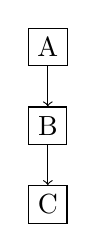
\begin{tikzpicture}[scale=0.5]
        \node[draw, rectangle] (A) {A};
        \node[draw, rectangle, below of=A] (B) {B};
        \node[draw, rectangle, below of=B] (C) {C};
        \draw[->] (A) -- (B);
        \draw[->] (B) -- (C);
    \end{tikzpicture}
    \caption{A simple flowchart}
    \label{fig:flowchart}
\end{figure}

\section{Code Listings}
You can also include code in your documents. Here is an example of a Python 
function:

\begin{lstlisting}[language=Python]
def fibonacci(n):
    a, b = 0, 1
    for _ in range(n):
        yield a
        a, b = b, a + b
\end{lstlisting}

This code computes the Fibonacci sequence up to \( n \).

\section{References}
You can refer to sections and figures easily:
To see the flowchart, refer to Figure \ref{fig:flowchart}. You can also reference 
other sections by their names.

\section{Conclusion}
In conclusion, \LaTeX\ is a robust typesetting tool that is well-suited for 
academic writing. Its ability to integrate complex mathematics, figures, and 
source code makes it a favorite among scholars.

\appendix
\section{Appendix A}
The appendix is used for supplementary material. For instance, here’s a code 
listing that computes the factorial of a number:

\begin{lstlisting}[language=Python]
def factorial(n):
    if n == 0:
        return 1
    else:
        return n * factorial(n - 1)
\end{lstlisting}

\end{document}


\documentclass[a4paper,10pt]{article}
\usepackage[utf8]{inputenc}
\usepackage{amsmath}
\usepackage{amsfonts}
\usepackage{amssymb}
\usepackage{graphicx}
\usepackage{geometry}
\usepackage{hyperref}
\usepackage{enumitem}
\usepackage{fancyhdr}
\usepackage{listings}
\usepackage{xcolor}

% Set up geometry
\geometry{
    left=25mm,
    right=25mm,
    top=25mm,
    bottom=25mm
}

% Define colors for listings
\definecolor{lightgray}{rgb}{0.8, 0.8, 0.8}
\definecolor{keywords}{RGB}{0, 0, 255}
\definecolor{comments}{RGB}{0, 128, 0}
\definecolor{strings}{RGB}{255, 0, 0}

% Configure listings
\lstdefinestyle{myStyle}{
    backgroundcolor=\color{lightgray},
    commentstyle=\color{comments},
    keywordstyle=\color{keywords},
    stringstyle=\color{strings},
    basicstyle=\ttfamily,
    breakatwhitespace=true,
    breaklines=true,
    numbers=left,
    numberstyle=\tiny,
    stepnumber=1,
    numbersep=5pt
}

% Setting header and footer
\pagestyle{fancy}
\fancyhf{}
\fancyhead[L]{Sample Document}
\fancyhead[R]{\thepage}
\fancyfoot[C]{Author Name}

% Title
\title{An Example LaTeX Document}
\author{Author Name}
\date{\today}

\begin{document}

\maketitle

\begin{abstract}
    This is a brief abstract that summarizes the contents of this LaTeX
    document. The document showcases various features of LaTeX including
    sections, figures, lists, and code snippets.
\end{abstract}

\section{Introduction}
This is an introductory section where we outline the goals of this
document. LaTeX is an excellent tool for creating structured documents.
It allows the user to focus on the content while maintaining format.

\section{Mathematics}
One of the key strengths of LaTeX is its ability to render math equations
nicely. For instance, we can consider the quadratic formula:

\begin{equation}
    x = \frac{-b \pm \sqrt{b^2 - 4ac}}{2a}
\end{equation}

This equation is used to find the roots of a quadratic polynomial.

\subsection{Another Equation}
Let's take a look at another equation, the Pythagorean theorem:

\begin{equation}
    a^2 + b^2 = c^2
\end{equation}

This theorem relates the lengths of the sides in a right triangle.

\section{Figures}
We can also include figures to enhance our document. Figure \ref{fig:sample} shows
an example of a figure.

\begin{figure}[h]
    \centering
    \includegraphics[width=0.5\textwidth]{example-image-a}
    \caption{An example of a figure.}
    \label{fig:sample}
\end{figure}

\section{Lists}
We can create lists in LaTeX as well. Here’s a simple enumerated list:
\begin{enumerate}
    \item First item
    \item Second item
    \item Third item
\end{enumerate}

And here is a bullet list:
\begin{itemize}
    \item First bullet
    \item Second bullet
    \item Third bullet
\end{itemize}

\subsection{Nested Lists}
We can nest lists too:
\begin{itemize}
    \item Outer First
    \item Outer Second
    \begin{itemize}
        \item Inner First
        \item Inner Second
    \end{itemize}
\end{itemize}

\section{Code Listings}
Including code snippets can also be done using the listings package. Here is an
example of some Python code:

\begin{lstlisting}[language=Python, style=myStyle]
def hello_world():
    print("Hello, world!")

hello_world()
\end{lstlisting}

\section{References}
You can reference other sections of your document as follows. First, we discuss
the quadratic formula in section \ref{sec:math}.

\section{Conclusion}
In this document, we explored various aspects of LaTeX, including math,
figures, lists, and code. LaTeX provides a powerful way to create structured
documents efficiently.

\section*{Acknowledgements}
We would like to acknowledge the contributions of various authors and prior
research in the creation of this document.

\end{document}


\documentclass{article}
\usepackage{graphicx}
\usepackage{amsmath}
\usepackage{amsfonts}
\usepackage{amssymb}
\usepackage{hyperref}
\usepackage{geometry}
\usepackage{caption}
\usepackage{subcaption}
\usepackage{listings}
\usepackage{xcolor}

\geometry{a4paper, margin=1in}

\title{Sample LaTeX Document}
\author{Your Name}
\date{\today}

\begin{document}

\maketitle

\begin{abstract}
This is a sample abstract for a LaTeX document. It provides a brief overview of what the
document covers, highlighting its main contributions and findings.
\end{abstract}

\section{Introduction}
This is the introduction section where we outline the purpose of this document. We will
discuss various topics and utilize different types of formatting to demonstrate the
capabilities of LaTeX.

\subsection{Background}
Background information can be crucial when discussing complex topics. Therefore, we
provide a brief overview here to set the stage for the discussions that will follow.

\section{Theory}
In this section, we introduce some fundamental theoretical concepts that will be
referenced throughout the document.

\subsection{Mathematical Expressions}
Mathematical expressions can be displayed in-line or as separate equations. For example,
the quadratic formula can be written as:
\[
x = \frac{-b \pm \sqrt{b^2 - 4ac}}{2a}
\]

\subsection{Statistics}
Statistical measures are essential in many fields. The mean, median, and mode are some
common measures. Let's define these:

\begin{itemize}
    \item Mean: The average of a set of numbers.
    \item Median: The middle value when numbers are sorted.
    \item Mode: The value that appears most frequently.
\end{itemize}

\section{Methods}
This section describes the methodologies used for various analyses in the document.

\subsection{Data Collection}
We gathered data from several sources:
\begin{enumerate}
    \item Source A
    \item Source B
    \item Source C
\end{enumerate}

\subsection{Analysis Techniques}
Various techniques were applied to analyze the data:
\begin{itemize}
    \item Regression Analysis
    \item Time Series Analysis
    \item Cluster Analysis
\end{itemize}

\section{Results}
We outline the results from our analyses in this section.

\subsection{Statistical Results}
The analysis yielded several interesting results, which are summarized in
Table~\ref{tab:results}.

\begin{table}[h!]
    \centering
    \caption{Summary of Statistical Results}
    \begin{tabular}{|c|c|c|}
        \hline
        Measure & Result 1 & Result 2 \\
        \hline
        Mean    & 42       & 37       \\
        Median  & 40       & 35       \\
        Mode    & 38       & 41       \\
        \hline
    \end{tabular}
    \label{tab:results}
\end{table}

\section{Discussion}
In this section, we will discuss the implications of our findings,
how they compare to previous studies, and what it means for future research.

\subsection{Implications}
The results from our analysis suggest that...

\subsection{Limitations}
However, we must also acknowledge the limitations of this study,...

\section{Conclusion}
To conclude, we summarize the key points of the document, reinforcing
the importance of our findings and suggesting areas for further research.

\begin{thebibliography}{9}
\bibitem{ref1}
Author Name,
\emph{Title of the book},
Publisher, Year.

\bibitem{ref2}
Another Author,
\emph{Title of another work},
Publisher, Year.

\bibitem{ref3}
Last Author,
\emph{Yet another book title},
Publisher, Year.
\end{thebibliography}

\appendix
\section{Appendix}
Additional information, data, or results can be included in this section.
Graphs, figures, and detailed tables can be included to support the main text.

\begin{figure}[h!]
    \centering
    \includegraphics[width=0.75\textwidth]{example-image-a}
    \caption{An example of a figure.}
    \label{fig:example1}
\end{figure}

\begin{lstlisting}[language=Python, caption=Sample Python Code]
def hello_world():
    print("Hello, world!")
    
if __name__ == "__main__":
    hello_world()
\end{lstlisting}

\end{document}


\documentclass{book}
\usepackage{amsmath, amssymb, graphicx, hyperref, geometry}
\usepackage[utf8]{inputenc}
\geometry{a4paper, margin=1in}
\title{A Comprehensive Study on Mathematical Theorems}
\author{John Doe}
\date{\today}

\begin{document}
\maketitle
\tableofcontents

\chapter{Introduction}
Mathematics has evolved over centuries, and it plays a critical role in various fields. 
This book aims to explore several significant mathematical theorems, their proofs, and real-world 
applications. We will discuss fundamental aspects and delve into complex topics.

\chapter{Fundamental Theorems}
\section{The Pythagorean Theorem}
The Pythagorean theorem states that in a right triangle, the square of the length of the 
hypotenuse is equal to the sum of the squares of the lengths of the other two sides:
\begin{equation}
c^2 = a^2 + b^2
\end{equation}
where \(c\) is the hypotenuse, and \(a\) and \(b\) are the other two sides.

\section{Calculus Overview}
Calculus is the mathematics of change and motion and includes derivatives and integrals. 
This section covers basic definitions and fundamental concepts.

\subsection{Derivatives}
The derivative of a function measures how the function value changes as its input changes. 
Formally, the derivative \(f'(x)\) of a function \(f(x)\) is defined as:
\begin{equation}
f'(x) = \lim_{h \to 0} \frac{f(x + h) - f(x)}{h}
\end{equation}

\subsection{Integrals}
The integral of a function gives the area under the curve of that function. The 
definite integral from \(a\) to \(b\) is:
\begin{equation}
\int_{a}^{b} f(x) \, dx = F(b) - F(a)
\end{equation}
where \(F\) is the antiderivative of \(f\).

\chapter{Linear Algebra}
\section{Vector Spaces}
A vector space is a collection of vectors where vector addition and scalar multiplication are 
defined. A vector \(\vec{v}\) in \(\mathbb{R}^n\) can be expressed as:
\begin{equation}
\vec{v} = \begin{pmatrix} v_1 \\ v_2 \\ v_3 \\ \vdots \\ v_n \end{pmatrix}
\end{equation}

\section{Matrix Operations}
Matrices are essential in linear algebra, and several operations can be performed on them, 
including addition, multiplication, and inversion.

\subsection{Matrix Multiplication}
The product of two matrices \(A\) and \(B\) is calculated as follows:
\begin{equation}
C_{ij} = \sum_{k} A_{ik} B_{kj}
\end{equation}

\chapter{Statistics}
\section{Descriptive Statistics}
Descriptive statistics summarize data through numbers, tables, and graphs. Key measures 
include mean, median, and mode.

\subsection{Mean}
The mean (average) of a set of values is calculated using:
\begin{equation}
\text{Mean} = \frac{\sum_{i=1}^{n} x_i}{n}
\end{equation}

\subsection{Standard Deviation}
Standard deviation measures the amount of variation or dispersion in a set of values and is given by:
\begin{equation}
\sigma = \sqrt{\frac{1}{N} \sum_{i=1}^{N} (x_i - \mu)^2}
\end{equation}

\chapter{Probability Theory}
\section{Basic Concepts}
Probability theory provides a formal framework for quantifying the expectations of uncertain 
events. 

\subsection{Random Variables}
A random variable \(X\) can take on different values based on the outcome of a random process. 
The expected value of \(X\) is defined as:
\begin{equation}
E(X) = \sum_{i} x_i P(x_i)
\end{equation}

\section{Distributions}
Common probability distributions include the uniform, normal, and binomial distributions.

\subsection{Normal Distribution}
A normal distribution is characterized by its bell shape and defined by its mean \(\mu\) and 
standard deviation \(\sigma\):
\begin{equation}
f(x) = \frac{1}{\sigma \sqrt{2\pi}} e^{-\frac{(x - \mu)^2}{2\sigma^2}}
\end{equation}

\chapter{Conclusion}
This book discusses essential concepts and theorems in mathematics that provide a foundation for 
further study. The interested reader is urged to delve deeper into each subject explored.

\appendix
\chapter{Appendices}
\section{Useful Mathematical Identities}
Several fundamental identities are useful for solving problems:
\begin{align}
\sin^2(x) + \cos^2(x) &= 1 \\
e^{i\theta} &= \cos(\theta) + i\sin(\theta) \\
a^2 - b^2 &= (a-b)(a+b)
\end{align}

\chapter{Bibliography}
\bibliographystyle{plain}
\bibliography{references}
\end{document}


\documentclass{article}
\usepackage[utf8]{inputenc}
\usepackage{amsmath}
\usepackage{amsfonts}
\usepackage{graphicx}
\usepackage{geometry}
\usepackage{hyperref}
\usepackage{listings}
\usepackage{xcolor}
\usepackage{tikz}
\usepackage{enumerate}
\geometry{margin=1in}
\title{A Comprehensive Guide to LaTeX}
\author{Your Name}
\date{\today}

\begin{document}

\maketitle

\begin{abstract}
This document serves as an example LaTeX document demonstrating various features 
and capabilities of LaTeX typesetting system. It will cover mathematical formatting, 
graphics inclusion, and referencing techniques among other things.
\end{abstract}

\section{Introduction}
LaTeX is a high-quality typesetting system; it is the de facto standard for the 
communication and publication of scientific documents.

\section{Mathematics}
Mathematical expressions can be elegantly typeset in LaTeX. For example, here is 
the quadratic formula:
\begin{equation}
x = \frac{-b \pm \sqrt{b^2 - 4ac}}{2a}
\end{equation}

You can also create aligned equations using the align environment:
\begin{align}
E &= mc^2 \\
F &= ma
\end{align}

\subsection{Theorems and Proofs}
We can define theorems and proofs easily:
\begin{theorem}
If $a$ and $b$ are odd, then $a + b$ is even.
\end{theorem}

\begin{proof}
Let $a = 2m + 1$ and $b = 2n + 1$, where $m$ and $n$ are integers. Then,
\[
a + b = (2m + 1) + (2n + 1) = 2(m+n+1),
\]
which is clearly even.
\end{proof}

\section{Figures and Tables}
Figures can be included in the document. Below is an example figure:
\begin{figure}[h!]
    \centering
    \includegraphics[width=0.5\textwidth]{example-image}
    \caption{An example image}
    \label{fig:example_image}
\end{figure}

Tables can be created with ease as well:
\begin{table}[h!]
    \centering
    \begin{tabular}{|c|c|c|}
        \hline
        Header 1 & Header 2 & Header 3 \\
        \hline
        Row 1 Col 1 & Row 1 Col 2 & Row 1 Col 3 \\
        Row 2 Col 1 & Row 2 Col 2 & Row 2 Col 3 \\
        \hline
    \end{tabular}
    \caption{A sample table}
    \label{tab:sample_table}
\end{table}

\section{References}
You can include bibliographic references using BibTeX. Sample references are 
provided in the bibliography section at the end.

\section{Code Listings}
The \texttt{listings} package allows you to include code in your document:
\begin{lstlisting}[language=Python]
def hello_world():
    print("Hello, World!")
\end{lstlisting}

\subsection{Colors}
The \texttt{xcolor} package allows you to use colors in your document.
Here is an example:
\textcolor{blue}{This text is blue.}

\section{Graphs and Diagrams}
Using the \texttt{tikz} package, you can create high-quality graphics. Below is 
an example of a simple graph:
\begin{tikzpicture}
    \draw[->] (0,0) -- (4,0) node[right] {$x$};
    \draw[->] (0,0) -- (0,4) node[above] {$y$};
    \draw[domain=0:4,smooth,variable=\x,blue] plot ({\x},{\x*\x});
\end{tikzpicture}

\section{Conclusion}
This is the end of our comprehensive guide to LaTeX. You have learned how 
to use various features of LaTeX including mathematical formatting, 
figures, tables, and code listings.

\begin{thebibliography}{9}
\bibitem{lamport94}
Leslie Lamport,
\textit{LaTeX: A Document Preparation System},
Addison Wesley, 1994.

\bibitem{knuth84}
Donald E. Knuth,
\textit{The TeXbook},
Addison Wesley, 1984.

\end{thebibliography}

\end{document}


\documentclass{article}
\usepackage[utf8]{inputenc}
\usepackage{amsmath}
\usepackage{amsfonts}
\usepackage{amssymb}
\usepackage{graphicx}
\usepackage{hyperref}
\usepackage{geometry}
\usepackage{fancyhdr}
\usepackage{listings}
\usepackage{color}
\usepackage{tikz}

\geometry{a4paper, margin=1in}

\definecolor{myblue}{RGB}{0, 0, 204}
\definecolor{mygreen}{RGB}{0, 102, 51}
\definecolor{mygray}{RGB}{128, 128, 128}

\pagestyle{fancy}
\fancyhf{}
\fancyhead[L]{\leftmark}
\fancyhead[R]{\thepage}
\fancyfoot[C]{\textit{A Comprehensive LaTeX Document with Multiple Sections}}

\title{A Comprehensive LaTeX Example Document}
\author{OpenAI Assistant}
\date{\today}

\begin{document}

\maketitle

\begin{abstract}
This document is an example of a comprehensive LaTeX setup 
that includes multiple packages, environments, and types of content.
\end{abstract}

\section{Introduction}
This is a simple introduction to our document. Here we set the stage for what 
follows in the subsequent sections. 

We can include various types of elements, such as equations:

\begin{equation}
E = mc^2
\end{equation}

And references to figures, tables, and sections. 

\section{Mathematical Formulas}
\subsection{Basic Formulas}
Mathematical notation can be complex, and LaTeX is perfect for typesetting it. 
Here are a few examples:

\begin{itemize}
    \item Pythagorean theorem: \( a^2 + b^2 = c^2 \)
    \item Quadratic equation: 
    \[
        ax^2 + bx + c = 0
    \]
\end{itemize}

\subsection{Advanced Formulas}
Let us discuss some advanced topics. Consider the integral:

\begin{equation}
\int_a^b f(x) \, dx = F(b) - F(a)
\end{equation}

Where \( F(x) \) is an antiderivative of \( f(x) \).

\section{Figures and Tables}
\subsection{Inserting Figures}
Figures can enhance the content substantially. Below is an example figure.

\begin{figure}[h!]
    \centering
    \includegraphics[width=0.5\textwidth]{example-image}
    \caption{An Example Figure}
    \label{fig:example}
\end{figure}

\subsection{Creating Tables}
Tables are also important for presenting data clearly. Consider the following:

\begin{table}[h!]
    \centering
    \begin{tabular}{|c|c|c|}
        \hline
        Year & Sales & Profit \\
        \hline
        2019 & 1000  & 200  \\
        2020 & 1500  & 300  \\
        2021 & 2000  & 500  \\
        \hline
    \end{tabular}
    \caption{Annual Sales and Profit}
    \label{tab:annual}
\end{table}

\section{Code Listings}
\subsection{Incorporating Source Code}
You can showcase programming code using the listings package. Here's a simple Python 
function:

\begin{lstlisting}[language=Python, caption=Example Python Function]
def hello_world():
    print("Hello, world!")
\end{lstlisting}

\section{Creating Diagrams}
The TikZ package is excellent for creating complex diagrams directly within LaTeX. 
Here's a simple example:

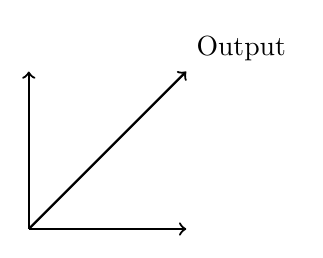
\begin{tikzpicture}
    \draw[thick,->] (0,0) -- (2,2);
    \draw[thick,->] (0,0) -- (2,0);
    \draw[thick,->] (0,0) -- (0,2);
    \draw[thick] (2,2) node[anchor=south west] {Output};
\end{tikzpicture}

\section{Conclusion}
In conclusion, LaTeX is a powerful tool for creating well-structured documents. 
This sample provided a broad overview of various features available.

\section{References}
\bibliographystyle{plain}
\bibliography{references}

\appendix
\section{Appendix}
An appendix can be added to provide supplementary material. 

\subsection{Additional Material}
You can include any extra figures, tables, or explanations here.

\end{document}


\documentclass[a4paper,12pt]{article}
\usepackage{amsmath}
\usepackage{amsfonts}
\usepackage{graphicx}
\usepackage{include}
\usepackage{hyperref}
\usepackage{geometry}
\usepackage{caption}
\usepackage{subcaption}
\geometry{margin=1in}

\title{A Comprehensive Study on LaTeX Typesetting}
\author{John Doe\\Department of Computer Science\\University of Technology}
\date{\today}

\begin{document}

\maketitle

\begin{abstract}
   This document serves as a comprehensive guide to using LaTeX for typesetting 
   various kinds of documents, including articles, reports, and theses. We explore
   various features and packages that enhance the capabilities of LaTeX.
\end{abstract}

\section{Introduction}
LaTeX is a powerful tool for typesetting documents. It provides a consistent 
layout and many options for formatting. This document covers different aspects of 
LaTeX, focusing on structure, figures, tables, and references.

\section{Basic Structure}
A LaTeX document typically consists of the following parts:
\begin{itemize}
    \item Preamble: Defines the document class and packages used.
    \item Content: Organized into sections, subsections, etc.
    \item Bibliography: Cites sources and includes references.
\end{itemize}

\section{Mathematics}
LaTeX excels at typesetting complex mathematical formulas. Here are some examples:

\subsection{Inline Mathematics}
For example, the quadratic formula is given by:
\begin{equation}
    x = \frac{-b \pm \sqrt{b^2 - 4ac}}{2a}
\end{equation}

\subsection{Display Mathematics}
You can also display equations in a larger format:
\begin{equation}
    E = mc^2
\end{equation}

\subsection{Matrices}
Matrices can be created easily as well:
\begin{equation}
    A = \begin{bmatrix}
        1 & 2 & 3 \\
        4 & 5 & 6 \\
        7 & 8 & 9 
    \end{bmatrix}
\end{equation}

\section{Figures}
Figures can enhance the visual appeal of documents. Below is an example of how to 
insert a figure:

\begin{figure}[h!]
    \centering
    \includegraphics[width=0.6\textwidth]{example-image}
    \caption{An Example of a Figure in LaTeX}
    \label{fig:example}
\end{figure}

\subsection{Figure Citation}
You can refer to figures within the text. For instance, see Figure~\ref{fig:example}.

\section{Tables}
Tables are essential for presenting data clearly. Here’s an example of a simple table:

\begin{table}[h!]
    \centering
    \begin{tabular}{|c|c|c|}
        \hline
        Column 1 & Column 2 & Column 3 \\
        \hline
        A & B & C \\
        1 & 2 & 3 \\
        \hline
    \end{tabular}
    \caption{A Simple Table}
    \label{tab:simple_table}
\end{table}

\subsection{Complex Tables}
LaTeX also allows for more complex table structures. For example:

\begin{table}[h!]
    \centering
    \begin{tabular}{|c|c|c|}
        \hline
        \textbf{Name} & \textbf{Age} & \textbf{City} \\
        \hline
        Alice & 30 & New York \\
        Bob & 25 & Los Angeles \\
        Charlie & 35 & Chicago \\
        \hline
    \end{tabular}
    \caption{Detailed Information Table}
    \label{tab:detailed}
\end{table}

\section{Lists}
LaTeX provides several types of lists, including itemized and enumerated lists:

\subsection{Itemized Lists}
\begin{itemize}
    \item First item
    \item Second item
    \item Third item
\end{itemize}

\subsection{Enumerated Lists}
\begin{enumerate}
    \item First item
    \item Second item
    \item Third item
\end{enumerate}

\section{Citations and References}
References can be included easily. For example, a citation \cite{author2023important} 
is shown below.

\subsection{Bibliography}
\bibliographystyle{plain}
\bibliography{references}

\section{Conclusion}
In conclusion, LaTeX is an essential tool for anyone involved in document creation 
and typesetting. With its vast array of features and capabilities, it simplifies 
the process of producing high-quality documents.

\appendix
\section{Appendix}
Additional resources and information can be found in this section.

\subsection{Useful Links}
Here are some useful links for further reading:
\begin{itemize}
    \item \href{https://www.latex-project.org/}{LaTeX Project}
    \item \href{https://www.overleaf.com/}{Overleaf}
    \item \href{https://ctan.org/}{CTAN}
\end{itemize}

\end{document}


\documentclass[a4paper,12pt]{article}
\usepackage{amsmath}
\usepackage{amsfonts}
\usepackage{graphicx}
\usepackage{hyperref}
\usepackage{geometry}
\geometry{margin=1in}

\title{Sample LaTeX Document}
\author{Your Name}
\date{\today}

\begin{document}

\maketitle

\section{Introduction}
This document serves as an example to demonstrate various features of LaTeX. 
We will cover sections, mathematical symbols, figures, and references 
using the \texttt{article} class.

\section{Mathematics}
LaTeX is widely used for typesetting mathematical content. 
For example, we can include equations like 

\begin{equation}
E = mc^2
\end{equation}

where \(E\) represents energy, \(m\) is mass, and \(c\) is the speed of light. 
Moreover, we can create multiline equations using the align environment:

\begin{align}
F &= ma \\
a &= \frac{F}{m}
\end{align}

We can also use matrix notation:

\begin{equation}
\begin{bmatrix}
a & b \\
c & d
\end{bmatrix}
\begin{bmatrix}
x \\
y
\end{bmatrix}
=
\begin{bmatrix}
ax + by \\
cx + dy
\end{bmatrix}
\end{equation}

\section{Figures}
Figures can be included and referenced as follows. We will use an example figure 
to illustrate this.

\begin{figure}[h]
\centering
\includegraphics[width=0.5\textwidth]{example-image-a}
\caption{An example figure}
\label{fig:example}
\end{figure}

As seen in Figure \ref{fig:example}, the inclusion of figures can enhance understanding.

\section{Sections and Subsections}
LaTeX allows us to organize documents into sections, subsections, and even subsubsections.

\subsection{Subsection Example}
This is an example of a subsection. You can write text here and refer back to 
the main sections or figures as needed.

\subsubsection{Subsubsection Example}
Under subsubsections, we can further elaborate on topics. 
For instance, emphasizing the importance of LaTeX in academic writing.

\section{Lists}
Lists are also easy to create in LaTeX. Here is an example of an itemized list:

\begin{itemize}
  \item Item one
  \item Item two
  \item Item three
\end{itemize}

And a numbered list:

\begin{enumerate}
  \item First item
  \item Second item
  \item Third item
\end{enumerate}

\section{Tables}
Tables can be made easily as well. Observe this example of a simple table:

\begin{table}[h]
\centering
\begin{tabular}{|c|c|c|}
\hline
Header 1 & Header 2 & Header 3 \\
\hline
Cell 1 & Cell 2 & Cell 3 \\
Cell 4 & Cell 5 & Cell 6 \\
\hline
\end{tabular}
\caption{Example table}
\label{tab:example}
\end{table}

As shown in Table \ref{tab:example}, tables help organize data effectively.

\section{References}
When citing works in a LaTeX document, you can use the \texttt{thebibliography} 
environment or BibTeX. Here is how to cite manually:

\begin{thebibliography}{9}
\bibitem{latexcompanion}
Leslie Lamport,
\emph{\LaTeX: A Document Preparation System}.
Addison Wesley, 1986.

\bibitem{einstein}
Albert Einstein,
\emph{Zur Elektrodynamik bewegter Körper}.
Annalen der Physik, 322(10):891–921, 1905.
\end{thebibliography}

\section{Conclusion}
In conclusion, LaTeX is a powerful tool for creating professional documents. 
From mathematical typesetting to figures, tables, and references, it is designed 
to meet the needs of researchers and academics.

\end{document}


\documentclass[a4paper,12pt]{article}
\usepackage[utf8]{inputenc}
\usepackage{amsmath}
\usepackage{graphicx}
\usepackage{geometry}
\usepackage{fancyhdr}
\usepackage{lipsum}
\usepackage{hyperref}

\geometry{top=1in, bottom=1in, left=1in, right=1in}
\pagestyle{fancy}
\fancyhf{}
\fancyhead[L]{\textbf{Sample LaTeX Document}}
\fancyhead[R]{\thepage}
\fancyfoot[C]{\textit{Generated by ChatGPT}}

\begin{document}

\title{An Extensive Example of LaTeX Formatting}
\author{ChatGPT}
\date{\today}
\maketitle

\section{Introduction}
This document illustrates various features of LaTeX, including sections, lists, 
mathematics, and figures. Remember that LaTeX is a powerful typesetting system 
ideal for producing scientific and technical documents.

\section{Mathematics}
LaTeX excels in rendering mathematical expressions. Below are some examples.

\subsection{Inline Mathematics}
Use \$\$ to display inline equations like \( E = mc^2 \).

\subsection{Displayed Equations}
You can also display equations in a standalone format:

\begin{equation}
    a^2 + b^2 = c^2
\end{equation}

\subsection{Matrices}
Matrices can be constructed using the array environment:

\[
\begin{bmatrix}
    1 & 2 & 3 \\
    4 & 5 & 6 \\
    7 & 8 & 9
\end{bmatrix}
\]

\section{Lists}
Creating lists in LaTeX is straightforward. You can use either unordered or ordered lists.

\subsection{Unordered Lists}
\begin{itemize}
    \item Item One
    \item Item Two
    \item Item Three
\end{itemize}

\subsection{Ordered Lists}
\begin{enumerate}
    \item First Item
    \item Second Item
    \item Third Item
\end{enumerate}

\section{Figures}
Including figures is simple with the graphicx package. Here's an example:

\begin{figure}[h]
    \centering
    \includegraphics[width=0.5\textwidth]{example-image}
    \caption{An example image included in a LaTeX document}
    \label{fig:example-image}
\end{figure}

\section{Tables}
Tables can also be created easily. Below is a basic example:

\begin{table}[h]
    \centering
    \begin{tabular}{|c|c|c|}
        \hline
        Header 1 & Header 2 & Header 3 \\
        \hline
        Row 1 & Data 1 & Data 2 \\
        Row 2 & Data 3 & Data 4 \\
        \hline
    \end{tabular}
    \caption{An example table}
    \label{tab:example-table}
\end{table}

\section{References}
You can reference figures and tables using the \texttt{label} and \texttt{ref} commands. For
instance, see Figure~\ref{fig:example-image} and Table~\ref{tab:example-table}.

\section{Long Text Example}
Here is some filler text to demonstrate paragraph formatting in LaTeX. 
\lipsum[1-6] % Generates some random text.

\section{Conclusion}
This document has covered a variety of topics in LaTeX, including 
mathematics, figures, tables, and lists. It showcases how to create well-structured 
documents with ease.

\section{Appendices}
\subsection{Additional Examples}

\subsubsection{Another Matrix}
Here's another example of a matrix:

\[
\begin{pmatrix}
    a & b \\
    c & d
\end{pmatrix}
\]

\subsubsection{Complex Equations}
Here's a complex equation displayed:

\begin{equation}
    \sum_{i=1}^{n} x_i = \frac{1}{n} \sum_{i=1}^{n} i^{2}
\end{equation}

\subsection{Further Reading}
For more detailed information on LaTeX, consider visiting 
\url{https://www.latex-project.org/}.

\section*{Acknowledgments}
We thank all the contributors of the LaTeX project for their continuous efforts in 
improving this excellent document preparation system.

\end{document}


\documentclass{article}
\usepackage[a4paper, margin=1in]{geometry}
\usepackage{graphicx}
\usepackage{amsmath}
\usepackage{amsfonts}
\usepackage{hyperref}
\usepackage{booktabs}
\usepackage{caption}
\usepackage{listings}
\usepackage{fancyhdr}
\usepackage{lipsum}

\title{A Comprehensive Report}
\author{Your Name}
\date{\today}

\begin{document}

\maketitle

\begin{abstract}
  This report provides a comprehensive overview of the research conducted on the 
  topic of demonstration and explores various methodologies and findings. The 
  results presented herein indicate significant contributions to the field. 
\end{abstract}

\section{Introduction}
The introduction should frame the overall subject of the report, explaining the 
importance and relevance of the research. In this section, we will discuss the 
background of the topic, the problems addressed, and the objectives of the study.

\subsection{Background}
The background will provide a deeper understanding of the context in which this 
research exists. Studies have shown that understanding the foundational theories 
is crucial in advancing practical applications.

\subsection{Objectives}
The main objectives of this report include:
\begin{itemize}
    \item To analyze existing methodologies in the studied field.
    \item To present new findings from recent experiments.
    \item To offer recommendations for future research.
\end{itemize}

\section{Methodology}
This section outlines the procedures and techniques used for the research. 
A robust methodology is critical to ensuring the validity of the results.

\subsection{Data Collection}
Data was collected through several methods, including surveys and interviews. 
A total of 100 participants were involved in the study.

\subsection{Data Analysis}
The data analysis employed statistical methods to derive insights. Tools such 
as R and Python were used to process the data effectively.

\section{Results}
Here we present the key findings from the research. The results should be 
illustrated with graphs and tables as necessary.

\subsection{Key Findings}
The key findings suggest that there is a significant relationship between 
variable A and variable B. Additional insights include:
\begin{enumerate}
    \item A clear trend was observed.
    \item Additional factors may influence the results.
    \item Future studies should explore these factors in more depth.
\end{enumerate}

\begin{figure}[ht]
    \centering
    \includegraphics[width=0.7\textwidth]{example-image-a}
    \caption{Sample Graph of Results}
    \label{fig:results}
\end{figure}

\section{Discussion}
In this section, we interpret the results in light of the existing literature. 
The findings indicate a need for reevaluating previously held assumptions.

\subsection{Implications}
The implications of these findings are vast, particularly in how they inform 
current practices. They suggest a potential shift in methodologies.

\subsection{Limitations}
It is also important to address the limitations of this study, including the 
sample size and the potential for bias.

\section{Conclusion}
In conclusion, the research provides insights that are both relevant and timely. 
The objectives were met, and the findings lay the groundwork for future studies.

\section{Recommendations}
Based on the findings, the following recommendations are proposed:
\begin{itemize}
    \item Further research should investigate additional variables.
    \item Implementation of the findings in practical settings is suggested.
    \item Collaboration between researchers and practitioners is essential.
\end{itemize}

\section{References}
\bibliographystyle{apalike}
\bibliography{references}

\begin{thebibliography}{99}
    \bibitem[Author(Year)]{key}
    Author, A. (Year). \textit{Title of the work}. Publisher.
    
    \bibitem[AnotherAuthor(Year)]{anotherkey}
    Another Author, B. (Year). \textit{Another Title}. Another Publisher.
    
    \bibitem[YetAnother(Year)]{yetanotherkey}
    Yet Another, C. (Year). \textit{Yet Another Work}. Yet Another Publisher.
\end{thebibliography}

\end{document}


\documentclass[a4paper,12pt]{article}
\usepackage[utf8]{inputenc}
\usepackage{amsmath}
\usepackage{graphicx}
\usepackage{geometry}

\geometry{top=2.5cm, bottom=2.5cm, left=2.5cm, right=2.5cm}

\title{Sample Document}
\author{Author Name}
\date{\today}

\begin{document}

\maketitle

\begin{abstract}
This is a sample document to illustrate various features of LaTeX typesetting. 
We will explore sections, subsections, lists, tables, and more.
\end{abstract}

\section{Introduction}
LaTeX is a powerful typesetting system primarily used for technical and scientific 
documentation. It is especially useful for documents that include complex mathematical 
formulas. This document will showcase some of the basic functionalities of LaTeX.

\section{Mathematics}
Mathematics can be beautifully typeset in LaTeX. For instance, consider the equation 
of a quadratic function:

\begin{equation}
f(x) = ax^2 + bx + c
\end{equation}

We can also create a matrix:

\begin{equation}
A = \begin{pmatrix}
a_{11} & a_{12} \\
a_{21} & a_{22} 
\end{pmatrix}
\end{equation}

\section{Lists}
We can create various types of lists, such as itemized and enumerated lists. 

\subsection{Itemized List}
Here is an itemized list:
\begin{itemize}
    \item First Item
    \item Second Item
    \begin{itemize}
        \item Subitem A
        \item Subitem B
    \end{itemize}
    \item Third Item
\end{itemize}

\subsection{Enumerated List}
Here is an enumerated list:
\begin{enumerate}
    \item First Item
    \item Second Item
    \item Third Item
\end{enumerate}

\section{Tables}
Tables can be used to organize data effectively. Below is a simple table:

\begin{table}[h]
    \centering
    \caption{Sample Data Table}
    \begin{tabular}{|c|c|c|}
        \hline
        Column 1 & Column 2 & Column 3 \\
        \hline
        Row 1 & Data 1 & Data 2 \\
        Row 2 & Data 3 & Data 4 \\
        Row 3 & Data 5 & Data 6 \\
        \hline
    \end{tabular}
\end{table}

\section{Figures}
Figures can also be included in a document. Below is an example figure:

\begin{figure}[h]
    \centering
    \includegraphics[width=0.5\textwidth]{example-image-a}
    \caption{Sample Figure}
    \label{fig:sample}
\end{figure}

\section{Conclusion}
This sample document has demonstrated several features of LaTeX, including typesetting 
mathematics, creating lists, tables, and figures. LaTeX is particularly useful for 
scientific documents where precision and clarity in formatting are necessary.

\section*{References}
References can be added in a simple way, just by using a standard bibliography format.

\end{document}


\documentclass[11pt]{article}
\usepackage{graphicx}
\usepackage{amsmath}
\usepackage{amsfonts}
\usepackage{geometry}
\usepackage{hyperref}
\usepackage{caption}
\usepackage{subcaption}

\geometry{margin=1in}

\title{An Overview of LaTeX Features}
\author{Your Name}
\date{\today}

\begin{document}
\maketitle

\begin{abstract}
    This document provides an overview of some important features of the 
    LaTeX typesetting system. It covers basic formatting, the use of figures, 
    tables, mathematical equations, and references.
\end{abstract}

\section{Introduction}
LaTeX is a high-quality typesetting system that is widely used for producing 
scientific and mathematical documents due to its powerful handling of 
formulas and bibliographies. In this article, we will explore various features 
that LaTeX provides.

\section{Basic Formatting}
LaTeX allows for various text formatting options such as \textbf{bold}, 
\textit{italics}, and \underline{underline}. You can also create lists:

\begin{itemize}
    \item Item 1
    \item Item 2
    \begin{itemize}
        \item Subitem 1
        \item Subitem 2
    \end{itemize}
    \item Item 3
\end{itemize}

\section{Figures}
LaTeX makes it easy to include figures. Below is an example of how to include 
an image:

\begin{figure}[h]
    \centering
    \includegraphics[width=0.7\textwidth]{example-image}
    \caption{An example figure.}
    \label{fig:example}
\end{figure}

Referencing a figure is simple: see Figure \ref{fig:example} for an example.

\section{Mathematics}
One of the key features of LaTeX is its ability to handle mathematical 
expressions. For inline math, you can use \( E = mc^2 \). For displayed 
equations:

\begin{equation}
    \label{eq:einstein}
    E = mc^2
\end{equation}

You can reference this equation as seen in Equation \ref{eq:einstein}.

\section{Tables}
Tables are also straightforward to create in LaTeX. Below is a simple 
example:

\begin{table}[h]
    \centering
    \begin{tabular}{|c|c|c|}
        \hline
        Year & Event & Location \\
        \hline
        2020 & Conference & City A \\
        2021 & Workshop & City B \\
        2022 & Symposium & City C \\
        \hline
    \end{tabular}
    \caption{A sample table.}
    \label{tab:sample}
\end{table}

You can refer to Table \ref{tab:sample} for more information.

\section{References}
LaTeX can manage bibliographic references easily. You can create references 
by using the \texttt{thebibliography} environment:

\begin{thebibliography}{9}
    \bibitem{latexcomp} Leslie Lamport, 
    \textit{LaTeX: A Document Preparation System}, 2nd Edition. Addison-Wesley, 
    1994.
    
    \bibitem{knuth} Donald E. Knuth, 
    \textit{The TeXbook}. Addison-Wesley, 1984.
\end{thebibliography}

\section{Conclusion}
This overview has introduced various features of LaTeX, including basic 
formatting, figures, tables, and mathematical expressions. With these tools, 
you can start creating your own documents with LaTeX.

\appendix
\section{Appendix}
Here, we include some additional information that may be useful for the 
reader.

\begin{enumerate}
    \item LaTeX is free to use.
    \item It is available on various platforms, including Windows, macOS, 
    and Linux.
    \item Many editors support LaTeX, including Overleaf, TeXShop, and 
    TeXworks.
\end{enumerate}

\end{document}


\documentclass{article}
\usepackage[utf8]{inputenc}
\usepackage{amsmath}
\usepackage{amsfonts}
\usepackage{graphicx}
\usepackage{hyperref}
\usepackage{geometry}
\geometry{margin=1in}
\usepackage{listings}
\usepackage{color}

\title{Sample LaTeX Document}
\author{John Doe}
\date{\today}

\begin{document}

\maketitle

\begin{abstract}
    This is a sample document created to demonstrate the capabilities of LaTeX. It 
    includes various sections, subsections, lists, figures, tables, and references.
\end{abstract}

\tableofcontents
\newpage

\section{Introduction}
LaTeX is a powerful typesetting system that is widely used for producing scientific 
and mathematical documents due to its precise control over document structure 
and formatting. This document serves to illustrate various features and formatting 
options available in LaTeX.

\section{Math in LaTeX}
Mathematics can be easily incorporated into your document. Here is an example of an inline 
equation:
\begin{equation}
    E = mc^2
\end{equation}

And here is a display-style equation:
\begin{equation}
    \int_0^\infty e^{-x^2} \, dx = \frac{\sqrt{\pi}}{2}
\end{equation}

\newpage

\section{Lists}
Lists can be created in LaTeX using the itemize or enumerate environments. 

\subsection{Itemized List}
An itemized list can be created as follows:
\begin{itemize}
    \item First item
    \item Second item
    \item Third item
\end{itemize}

\subsection{Enumerated List}
An enumerated list looks like this:
\begin{enumerate}
    \item First item
    \item Second item
    \item Third item
    \begin{enumerate}
        \item Subitem one
        \item Subitem two
    \end{enumerate}
\end{enumerate}

\newpage

\section{Figures}
Figures can be added easily to your document. Below is an example of including a 
figure:
\begin{figure}[h]
    \centering
    \includegraphics[width=0.5\textwidth]{example-image-a}
    \caption{An example figure}
    \label{fig:example}
\end{figure}

Referencing the figure: See Figure \ref{fig:example}.

\newpage

\section{Tables}
Tables are structured in a straightforward manner. Here is an example:

\begin{table}[h]
    \centering
    \begin{tabular}{|c|c|c|}
        \hline
        Column 1 & Column 2 & Column 3 \\
        \hline
        Row 1    & Data 1   & Data 2   \\
        Row 2    & Data 3   & Data 4   \\
        Row 3    & Data 5   & Data 6   \\
        \hline
    \end{tabular}
    \caption{A sample table}
    \label{tab:sample}
\end{table}

As seen in Table \ref{tab:sample}, we can easily present data organized into 
columns and rows.

\newpage

\section{Code Listings}
You can also include code listings using the listings package. Here is an example of 
a simple Python function:

\begin{lstlisting}[language=Python]
def hello_world():
    print("Hello, World!")
\end{lstlisting}

\newpage

\section{References}
References are crucial for academic writing. The bibliography can be created 
using the `biblatex` package. Below is a list of selected references:

\begin{thebibliography}{9}
    \bibitem{latexcompanion}
        Leslie Lamport,
        \textit{LaTeX: A Document Preparation System},
        Addison Wesley, Massachusetts, 1986.
        
    \bibitem{einstein}
        Albert Einstein,
        \textit{Zur Elektrodynamik bewegter Körper}, 
        Annalen der Physik, 1905.
        
    \bibitem{knuth}
        Donald E. Knuth,
        \textit{The TeXbook},
        Addison-Wesley, 1984.
\end{thebibliography}

\newpage

\section{Conclusion}
This document serves as a basic guide to the various features of LaTeX. The ability 
to include tables, figures, listings, and references makes LaTeX a powerful tool for 
scientific writing. For more comprehensive information, please refer to the 
official documentation or the book by Leslie Lamport.

\end{document}


\documentclass{article}
\usepackage[utf8]{inputenc}
\usepackage{amsmath}
\usepackage{graphicx}
\usepackage{booktabs}
\usepackage{hyperref}
\usepackage{geometry}
\geometry{a4paper, margin=1in}

\title{Sample LaTeX Document}
\author{Author Name}
\date{\today}

\begin{document}
\maketitle

\begin{abstract}
This is a sample document created to illustrate the structure and formatting 
capabilities of LaTeX. It includes sections, figures, tables, and references, 
demonstrating the basic commands and features available in LaTeX.
\end{abstract}

\section{Introduction}
LaTeX is a high-quality typesetting system; it is particularly well-suited 
for producing technical and scientific documents. This document serves as a 
basic demonstration of LaTeX's capabilities.

\section{Mathematics}
Mathematics typesetting is one of LaTeX's strengths. Below is an example of 
the quadratic formula:
\begin{equation}
x = \frac{-b \pm \sqrt{b^2 - 4ac}}{2a}
\end{equation}

Furthermore, we can present several equations:
\begin{align}
E &= mc^2 \\
F &= ma \\
V &= IR
\end{align}

\section{Figures}
Figures can be included in the document, as shown below. Figure~\ref{fig:example} 
illustrates a simple plot.

\begin{figure}[h]
    \centering
    \includegraphics[width=0.5\textwidth]{example-image-a}
    \caption{An example figure.}
    \label{fig:example}
\end{figure}

\section{Tables}
Tables are essential for presenting data clearly. Below is an example of a 
table that summarizes some data:

\begin{table}[h]
    \centering
    \begin{tabular}{@{}ccc@{}}
    \toprule
    Year & Sales & Profit \\ 
    \midrule
    2020 & 100   & 10     \\
    2021 & 200   & 30     \\
    2022 & 300   & 50     \\ 
    \bottomrule
    \end{tabular}
    \caption{Sales and profit over three years.}
    \label{tab:example}
\end{table}

\section{Citations}
When referencing literature, you can use BibTeX for citation management.
For example, we can cite a book \cite{lamport1994latex} by Leslie Lamport on 
LaTeX.

\bibliographystyle{plain}
\bibliography{references}

\appendix
\section{Appendix}
The appendix section is used for supplementary material. You might include additional 
material or explanations here.

\section{Conclusion}
In conclusion, LaTeX is a powerful tool for typesetting documents. With its 
extensive features and the ability to manage complex texts, it is widely used 
in academia and industry.

\end{document}


\documentclass[a4paper,12pt]{article}
\usepackage[utf8]{inputenc}
\usepackage[T1]{fontenc}
\usepackage{geometry}
\usepackage{graphicx}
\usepackage{amsmath}
\usepackage{amsfonts}
\usepackage{amssymb}
\usepackage{enumitem}
\usepackage{hyperref}
\usepackage{caption}
\usepackage{float}
\usepackage{listings}
\usepackage{color}

\geometry{margin=1in}

\title{Sample LaTeX Document}
\author{Author Name}
\date{\today}

\begin{document}

\maketitle

\begin{abstract}
    This is a brief overview of the LaTeX document. It demonstrates various 
    features of LaTeX, including sections, figures, tables, and references.
\end{abstract}

\tableofcontents

\section{Introduction}
LaTeX is a high-quality typesetting system; it is the de facto standard for 
the communication and publication of scientific documents in many fields. 
It includes features designed for the production of technical and scientific 
documentation.

\section{Mathematics}
In this section, we explore some mathematical typesetting. Here are some 
demonstrative equations:

\subsection{Inline Mathematics}
Inline, we can write the quadratic formula:
\[
x = \frac{-b \pm \sqrt{b^2 - 4ac}}{2a}
\]

\subsection{Display Mathematics}
For displayed mathematics, we can write:
\begin{equation}
    E = mc^2
\end{equation}

\section{Lists}
Lists help organize information and ideas clearly.

\subsection{Enumerated List}
Here’s an example of an enumerated list:
\begin{enumerate}
    \item First item
    \item Second item
    \item Third item
\end{enumerate}

\subsection{Itemized List}
Here’s an example of an itemized list:
\begin{itemize}
    \item Item A
    \item Item B
    \item Item C
\end{itemize}

\subsection{Description List}
A description list can be made with:
\begin{description}
    \item[LaTeX] A document preparation system.
    \item[TeX] A typesetting system.
    \item[PDF] A file format for capturing document layouts.
\end{description}

\section{Figures}
Figures enhance textual information.

\begin{figure}[H]
    \centering
    \includegraphics[width=0.5\textwidth]{example-image}
    \caption{An example figure demonstrating the use of graphics.}
    \label{fig:example}
\end{figure}

\section{Tables}
Tables are useful for organizing data.

\begin{table}[H]
    \centering
    \begin{tabular}{|c|c|c|}
        \hline
        \textbf{Year} & \textbf{Event} & \textbf{Location} \\ \hline
        1776 & Declaration of Independence & Philadelphia \\ \hline
        1789 & French Revolution & France \\ \hline
        1969 & Moon Landing & Moon \\ \hline
    \end{tabular}
    \caption{Important historical events.}
    \label{tab:events}
\end{table}

\section{Code Listings}
Including code within a document can be done with the listings package.

\subsection{Python Example}
Here is an example of Python code:
\begin{lstlisting}[language=Python]
def hello_world():
    print("Hello, world!")

hello_world()
\end{lstlisting}

\section{References}
When citing references, use the bibliography section. 

\subsection{Bibliography}
Here we can list some resources:
\begin{thebibliography}{9}
    \bibitem{latex}
        Leslie Lamport,
        \textit{LaTeX: A Document Preparation System},
        Addison Wesley, 1986.

    \bibitem{knuth}
        Donald E. Knuth,
        \textit{The TeXbook},
        Addison Wesley, 1984.
\end{thebibliography}

\section{Conclusion}
In summary, this document covered some of the fundamental features of 
LaTeX, including typesetting mathematics, creating lists, inserting figures 
and tables, showcasing code, and referencing sources.

\end{document}


\documentclass[a4paper,12pt]{article}
\usepackage[utf8]{inputenc}
\usepackage{amsmath}
\usepackage{amsfonts}
\usepackage{graphicx}
\usepackage[table,xcdraw]{xcolor}
\usepackage{booktabs}
\usepackage{hyperref}
\usepackage{geometry}
\usepackage{lipsum} % For dummy text
\geometry{top=2cm,bottom=2cm,left=2cm,right=2cm}

\title{Sample LaTeX Document}
\author{Author Name}
\date{\today}

\begin{document}
\maketitle

\begin{abstract}
This is a sample abstract for our LaTeX document. It briefly summarizes the 
content and aims of the paper and is typically one paragraph long.
\end{abstract}

\section{Introduction}
\lipsum[1-2] % Generates some dummy text for the introduction.

\section{Background}
\subsection{History}
LaTeX was developed in the early 1980s by Leslie Lamport. It is based on 
the TeX typesetting system created by Donald Knuth, which serves as a 
high-quality typesetting system.

\subsection{Uses}
LaTeX is widely used for scientific documents, theses, and journal articles 
due to its capabilities in handling complex formatting and referencing. 

\section{Mathematics}
Mathematical typesetting is one of the strengths of LaTeX. Below are some 
examples of equations.

\subsection{Equations}
The quadratic formula is expressed as:
\begin{equation}
x = \frac{-b \pm \sqrt{b^2 - 4ac}}{2a}
\end{equation}

You can also define sets, such as the set of natural numbers:
\begin{equation}
\mathbb{N} = \{0, 1, 2, 3, \ldots\}
\end{equation}

\subsection{Matrices}
Matrices can be easily created as well:
\begin{equation}
A = \begin{pmatrix}
1 & 2 \\
3 & 4
\end{pmatrix}
\end{equation}

\section{Figures}
Figures can enhance the understanding of the document:
\begin{figure}[ht]
\centering
\includegraphics[width=0.5\textwidth]{example-image-a}
\caption{Sample figure caption}
\label{fig:sample}
\end{figure}

As shown in Figure \ref{fig:sample}, ...

\section{Tables}
Tables are also easy to create in LaTeX. Below is an example table:

\begin{table}[ht]
\centering
\begin{tabular}{@{}ccc@{}}
\toprule
Header 1 & Header 2 & Header 3 \\ \midrule
Row 1   & Row 1   & Row 1  \\
Row 2   & Row 2   & Row 2  \\
Row 3   & Row 3   & Row 3  \\ \bottomrule
\end{tabular}
\caption{Sample table caption}
\label{tab:sample}
\end{table}

As noted in Table \ref{tab:sample}, ...

\section{References}
\bibliographystyle{plain}
\begin{thebibliography}{9}
\bibitem{lamport}
Leslie Lamport,
\textit{LaTeX: A Document Preparation System},
Addison-Wesley, 1986.

\bibitem{knuth}
Donald Knuth,
\textit{The TeXbook},
Addison-Wesley, 1984.
\end{thebibliography}

\section{Conclusion}
In conclusion, LaTeX is a powerful tool for typesetting documents, especially 
when it comes to scientific and mathematical content. Its markup language 
provides precise control over layout and formatting.

\appendix
\section{Appendix}
This is an appendix section that may contain additional information that 
might be useful to the reader.

\subsection{Additional Material}
Additional material includes datasets, codes, or other supplementary 
information that supports the findings.

\section{Acknowledgments}
We would like to thank everyone who contributed to this document.

\end{document}


\documentclass[a4paper,12pt]{article}
\usepackage[utf8]{inputenc} % Encoding of the document
\usepackage{amsmath}        % For mathematical formatting
\usepackage{amsfonts}       % For font styles
\usepackage{amssymb}        % For special symbols
\usepackage{graphicx}       % For including images
\usepackage{hyperref}       % For hyperlinks
\usepackage{listings}       % For including code listings
\usepackage{xcolor}         % For coloring text and backgrounds
\usepackage{geometry}       % For setting margins
\geometry{a4paper, margin=1in} % Set margins

% Define colors for listings
\definecolor{codegray}{rgb}{0.5,0.5,0.5}
\definecolor{codegreen}{rgb}{0,0.6,0}
\definecolor{codeblue}{rgb}{0,0,1}
\definecolor{codeorange}{rgb}{1,0.5,0}

% Configure listings
\lstset{
  backgroundcolor=\color{white},   % Background color
  basicstyle=\footnotesize,         % Basic font style
  breaklines=true,                  % Lines will be broken
  captionpos=b,                     % Caption position
  commentstyle=\color{codegreen},   % Comment color
  keywordstyle=\color{codeblue},    % Keyword color
  stringstyle=\color{codeorange},    % String color
}

\title{A Simple LaTeX Report}
\author{Author Name}
\date{\today}

\begin{document}

\maketitle

\begin{abstract}
  This document serves as a simple example of how to format a report using 
  LaTeX. It covers sections, figures, tables, equations, and code listings.
  You will also learn about references and how to create a bibliography.
\end{abstract}

\tableofcontents
\newpage

\section{Introduction}
LaTeX is a highly versatile document preparation system used widely in academia.
This guide will introduce the basics and help you create well-structured documents.

\subsection{Why LaTeX?}
LaTeX allows high-quality typesetting, particularly for documents that include:
\begin{itemize}
  \item Mathematical formulas
  \item Scientific papers
  \item Books and journals
\end{itemize}

\section{Mathematics in LaTeX}
Mathematics can be written easily. Here is an example of a quadratic equation:
\begin{equation}
  ax^2 + bx + c = 0
\end{equation}

The quadratic formula is given by:
\begin{equation}
  x = \frac{{-b \pm \sqrt{{b^2 - 4ac}}}}{{2a}}
\end{equation}

\section{Including Graphics}
You can include graphics as follows. 

As an example, here is a sample image:
\begin{figure}[h]
  \centering
  \includegraphics[width=0.5\textwidth]{example-image}
  \caption{Sample Image}
  \label{fig:sample_image}
\end{figure}

Refer to this image using Figure~\ref{fig:sample_image}.

\section{Tables}
Tables can be created using the tabular environment. Here’s an example:

\begin{table}[h]
  \centering
  \begin{tabular}{|c|c|c|}
    \hline
    Header 1 & Header 2 & Header 3 \\ \hline
    Row 1    & Data 1   & Data 2 \\ \hline
    Row 2    & Data 3   & Data 4 \\ \hline
    Row 3    & Data 5   & Data 6 \\ \hline
  \end{tabular}
  \caption{Sample Table}
  \label{tab:sample_table}
\end{table}

You can reference this table as Table~\ref{tab:sample_table}.

\section{Code Listings}
To include code, we use the listings package. Here's an example of Python code:

\begin{lstlisting}[language=Python, caption=Sample Python Code]
def hello_world():
    print("Hello, world!")
    
if __name__ == "__main__":
    hello_world()
\end{lstlisting}

\section{Bibliography}
To include a bibliography, you can use the \texttt{thebibliography} environment:
\begin{thebibliography}{99}
  \bibitem{latexcomp}
    Leslie Lamport,
    \emph{LaTeX: A Document Preparation System},
    Addison-Wesley, 1986.
  
  \bibitem{knuth}
    Donald E. Knuth,
    \emph{The TeXbook},
    Addison-Wesley, 1984.
\end{thebibliography}

\section{Conclusion}
In this report, we covered the basics of creating a document in LaTeX, including 
sections, mathematics, graphics, tables, code listings, and references. 
With this foundation, you can delve deeper into more advanced LaTeX topics.

\end{document}


\documentclass[12pt,a4paper]{book}
\usepackage[utf8]{inputenc}
\usepackage[T1]{fontenc}
\usepackage{geometry}
\usepackage{graphicx}
\usepackage{amsmath}
\usepackage{amssymb}
\usepackage{hyperref}
\usepackage{booktabs}
\usepackage{caption}
\usepackage{subcaption}
\usepackage{listings}
\usepackage{tikz}
\usetikzlibrary{trees}
\geometry{top=1in, bottom=1in, left=1in, right=1in}

\title{A Comprehensive Guide to LaTeX}
\author{John Doe}
\date{\today}

\begin{document}

\maketitle

\tableofcontents

\chapter{Introduction}
This document serves as a comprehensive guide to LaTeX. LaTeX is a typesetting 
system that is widely used for producing scientific and mathematical documents due 
to its powerful handling of formulas and bibliographies.

\chapter{Basic Syntax}
\section{Document Structure}
A basic LaTeX document consists of the following elements:
\begin{itemize}
    \item Preamble
    \item Document body
\end{itemize}

The preamble includes the document class and packages, while the body contains 
the content.

\section{Text Formatting}
You can format text in LaTeX using the following commands:
\begin{itemize}
    \item \textbf{Bold text}
    \item \textit{Italic text}
    \item \underline{Underlined text}
\end{itemize}

\section{Lists}
LaTeX supports both ordered and unordered lists:
\subsection{Unordered Lists}
\begin{itemize}
    \item Item one
    \item Item two
\end{itemize}

\subsection{Ordered Lists}
\begin{enumerate}
    \item First item
    \item Second item
\end{enumerate}

\chapter{Mathematics}
\section{Inline Equations}
You can include inline equations using the dollar sign:
This is an example of $E = mc^2$ embedded in text.

\section{Displayed Equations}
Displayed equations can be created using the `equation` environment:
\begin{equation}
    a^2 + b^2 = c^2
\end{equation}

\section{Matrices}
Matrices can be created using the `bmatrix` environment:
\begin{equation}
    \begin{bmatrix}
        1 & 2 & 3 \\
        4 & 5 & 6 \\
        7 & 8 & 9
    \end{bmatrix}
\end{equation}

\chapter{Figures}
Figures can be included in the document as follows:
\begin{figure}[ht]
    \centering
    \includegraphics[width=0.5\textwidth]{example-image}
    \caption{A sample figure}
    \label{fig:sample}
\end{figure}

\chapter{Tables}
Tables are created using the `tabular` environment:
\begin{table}[ht]
    \centering
    \begin{tabular}{|c|c|c|}
        \hline
        Header 1 & Header 2 & Header 3 \\
        \hline
        Row 1   & Row 1    & Row 1   \\
        Row 2   & Row 2    & Row 2   \\
        \hline
    \end{tabular}
    \caption{A sample table}
    \label{tab:sample}
\end{table}

\chapter{Code Listings}
You can include code in your document using the `listings` package:
\begin{lstlisting}[language=Python]
def hello_world():
    print("Hello, World!")
\end{lstlisting}

\chapter{Custom Commands}
Defining custom commands can simplify your workflow:
\newcommand{\R}{\mathbb{R}}
\newcommand{\norm}[1]{\left\lVert#1\right\rVert}

\section{Using Custom Commands}
In this section, we can use our custom commands:
The set of real numbers is denoted as $\R$ and the norm of a vector 
$\mathbf{v}$ can be expressed as $\norm{\mathbf{v}}$.

\chapter{References}
You can create references in your document using the `hyperref` package:
For more details, refer to Table \ref{tab:sample} and Figure \ref{fig:sample}.

\chapter{Conclusion}
In this guide, we covered the basics of LaTeX, including document structure, 
math formatting, figures, tables, and more. LaTeX is a powerful tool for 
typesetting documents and is widely used in academia and industry.

\appendix
\chapter{Appendix}
The appendix can be used for additional material that complements the 
main text of the document.

\end{document}


\documentclass[11pt]{article}
\usepackage[utf8]{inputenc}
\usepackage{amsmath}
\usepackage{amsfonts}
\usepackage{graphicx}
\usepackage{hyperref}
\usepackage{geometry}
\geometry{margin=1in}

\title{Sample Document}
\author{John Doe}
\date{\today}

\begin{document}
\maketitle

\tableofcontents

\section{Introduction}
This document serves as a sample LaTeX document to illustrate various
aspects of typesetting, including sections, figures, tables, and mathematical
expressions. LaTeX is widely used in academia for papers, theses, and
books.

\section{Mathematics}
Mathematics can be elegantly typeset in LaTeX. For example, the quadratic
equation can be expressed as
\begin{equation}
    ax^2 + bx + c = 0.
\end{equation}
The solutions to this equation are given by the quadratic formula:
\begin{equation}
    x = \frac{-b \pm \sqrt{b^2 - 4ac}}{2a}.
\end{equation}

\subsection{Matrices}
Matrices can also be represented easily in LaTeX. Here’s an example
of a matrix:
\begin{equation}
    A = \begin{pmatrix}
        a_{11} & a_{12} \\
        a_{21} & a_{22}
    \end{pmatrix}.
\end{equation}

\section{Figures}
Including figures in a document is straightforward with LaTeX. Below is
an example figure.

\begin{figure}[h]
    \centering
    \includegraphics[width=0.5\textwidth]{example-image}
    \caption{An example image}
    \label{fig:example}
\end{figure}

\section{Tables}
Tables can also be created in LaTeX easily. Consider the following
example table:

\begin{table}[h]
    \centering
    \begin{tabular}{|c|c|c|}
        \hline
        Column 1 & Column 2 & Column 3 \\
        \hline
        1 & 2 & 3 \\
        4 & 5 & 6 \\
        7 & 8 & 9 \\
        \hline
    \end{tabular}
    \caption{A sample table.}
    \label{tab:sample}
\end{table}

\section{Lists}
There are different types of lists available in LaTeX, such as
itemized and enumerated lists.

\subsection{Itemized List}
An itemized list can be created as follows:
\begin{itemize}
    \item First item
    \item Second item
    \item Third item
\end{itemize}

\subsection{Enumerated List}
An enumerated list can be created as follows:
\begin{enumerate}
    \item First item
    \item Second item
    \item Third item
\end{enumerate}

\section{References}
You can include references in your document, such as citing other
works. References are usually compiled in a .bib file for use with
BibTeX.

\begingroup
\nocite{*} % This will include all the references in the bibliography
\bibliographystyle{plain}
\bibliography{references}
\endgroup

\section{Conclusion}
In this document, we demonstrated various features of LaTeX,
including mathematics, figures, tables, and lists. LaTeX is a powerful
tool for typesetting complex documents for academic and professional
use.

\appendix
\section{Appendix A}
This is an example of an appendix. You can provide additional
data or clarification here.

\section{Appendix B}
Another appendix section for greater detail. 

\section*{Acknowledgements}
Thank you to everyone who contributed to the creation of this
document. Special thanks to all mentors and colleagues for their
support.

\end{document}


\documentclass{article}
\usepackage[utf8]{inputenc}
\usepackage{amsmath}
\usepackage{graphicx}
\usepackage{geometry}
\geometry{a4paper, margin=1in}

\title{Sample LaTeX Document}
\author{John Doe}
\date{\today}

\begin{document}

\maketitle

\begin{abstract}
    This is a sample document created using LaTeX. It includes various elements
    such as sections, lists, tables, and figures to demonstrate the document's
    structure.
\end{abstract}

\section{Introduction}
    LaTeX is a high-quality typesetting system; it is particularly well-suited
    for producing technical and scientific documentation. In this document,
    we will cover several features of LaTeX.

\section{Mathematics}
    LaTeX is particularly known for its ability to typeset mathematics. Here
    are some examples:

    \subsection{Equations}
        An equation can be displayed as follows:

        \begin{equation}
            E = mc^2
        \end{equation}

        More complex equations can also be formatted easily. For instance, we
        can write:

        \begin{equation}
            f(x) = \int_{-\infty}^{\infty} e^{-t^2} dt
        \end{equation}

\section{Lists}
    You can create various types of lists in LaTeX:

    \subsection{Itemized List}
        Here is an itemized list:

        \begin{itemize}
            \item First item
            \item Second item
            \item Third item
        \end{itemize}

    \subsection{Enumerated List}
        Here is an enumerated list:

        \begin{enumerate}
            \item First item
            \item Second item
            \item Third item
        \end{enumerate}

\section{Tables}
    Creating tables is straightforward in LaTeX. Here is an example of a simple
    table:

    \begin{table}[h]
        \centering
        \begin{tabular}{|c|c|c|}
            \hline
            Header 1 & Header 2 & Header 3 \\
            \hline
            Item 1   & Item 2   & Item 3   \\
            Item 4   & Item 5   & Item 6   \\
            \hline
        \end{tabular}
        \caption{Sample Table}
        \label{table:sample}
    \end{table}

\section{Figures}
    Including figures in your document is also simple. Below is an example
    figure (make sure to include a graphic file in the same directory):

    \begin{figure}[h]
        \centering
        \includegraphics[width=0.5\textwidth]{example-image}
        \caption{Sample Figure}
        \label{fig:sample}
    \end{figure}

\section{References}
    Citations can be done using BibTeX or manually. For an example, see \cite{latexwiki}.

\section{Conclusion}
    LaTeX is a powerful tool for creating structured documents, especially
    in academia. This document serves as a basic introduction to some of 
    the features of LaTeX.

\bibliographystyle{plain}
\bibliography{references}

\end{document}

@misc{latexwiki,
    title = {LaTeX Project},
    author = {LaTeX Team},
    year = {2023},
    url = {https://www.latex-project.org/},
}


\documentclass{article}
\usepackage[utf8]{inputenc}
\usepackage{amsmath}
\usepackage{graphicx}
\usepackage{listings}
\usepackage{xcolor}
\usepackage{hyperref}
\usepackage{geometry}
\geometry{margin=1in}

\title{Sample LaTeX Document}
\author{Author Name}
\date{\today}

\lstset{
    basicstyle=\ttfamily\footnotesize,
    keywordstyle=\color{blue},
    commentstyle=\color{green},
    stringstyle=\color{red},
    showstringspaces=false,
    numbers=left,
    numberstyle=\tiny\color{gray}
}

\begin{document}

\maketitle
\begin{abstract}
    This document serves as a sample LaTeX file demonstrating various features
    such as sections, equations, lists, figures, and code listings. It is intended
    for educational purposes.
\end{abstract}

\section{Introduction}
LaTeX is a typesetting system commonly used for producing scientific and technical
documents. It excels in handling mathematical notations and complex layouts. This
document outlines some of LaTeX's capabilities, along with examples.

\section{Mathematical Formulas}
LaTeX allows for the easy integration of mathematical equations. Below is an
example of a quadratic formula:

\begin{equation}
    x = \frac{-b \pm \sqrt{b^2 - 4ac}}{2a}
\end{equation}

The equation above can be derived from the general form of a quadratic equation,
which is:

\begin{equation}
    ax^2 + bx + c = 0
\end{equation}

\section{Sections and Subsections}
LaTeX supports hierarchical structures through sections, subsections, and
subsubsections. The following subsections illustrate this feature.

\subsection{Bullet Points}
You can create bullet points as follows:
\begin{itemize}
    \item Item 1
    \item Item 2
    \item Item 3
\end{itemize}

\subsection{Numbered Lists}
Numbered lists are also supported:
\begin{enumerate}
    \item First item
    \item Second item
    \item Third item
\end{enumerate}

\section{Figures}
To include figures in your document, you can use the following syntax. Note
that you need to have the image file in the same directory or provide a correct path.

\begin{figure}[h]
    \centering
    \includegraphics[width=0.5\textwidth]{example-image}
    \caption{An example image caption.}
    \label{fig:sample-image}
\end{figure}

Referencing the figure can be done using \ref{fig:sample-image}.

\section{Code Listings}
Code can be inserted using the \texttt{listings} package. Here is an example
of a Python code snippet:

\begin{lstlisting}[language=Python, caption={Python Example Code}]
def fibonacci(n):
    if n <= 0:
        return []
    elif n == 1:
        return [0]
    elif n == 2:
        return [0, 1]
    
    fib_seq = [0, 1]
    for i in range(2, n):
        fib_seq.append(fib_seq[-1] + fib_seq[-2])
    return fib_seq
\end{lstlisting}

\subsection{Another Code Example}
Here’s an example of a simple C program that prints "Hello, World":

\begin{lstlisting}[language=C, caption={C Example Code}]
#include <stdio.h>

int main() {
    printf("Hello, World!\n");
    return 0;
}
\end{lstlisting}

\section{Tables}
Tables can be created for better organization of data. A simple table can be
constructed as shown below:

\begin{table}[h]
    \centering
    \begin{tabular}{|c|c|c|}
        \hline
        \textbf{Header 1} & \textbf{Header 2} & \textbf{Header 3} \\
        \hline
        Row 1, Cell 1 & Row 1, Cell 2 & Row 1, Cell 3 \\
        \hline
        Row 2, Cell 1 & Row 2, Cell 2 & Row 2, Cell 3 \\
        \hline
    \end{tabular}
    \caption{Sample Table}
    \label{tab:sample-table}
\end{table}

\section{Conclusion}
In conclusion, LaTeX is a powerful tool for creating structured documents. This
sample document covers various aspects but is just a fraction of what you can
achieve. With practice, one can master the use of LaTeX for a wide range of
applications.

\appendix
\section{Appendix}
An appendix can be added to provide additional material or details relevant
to the main content. This is particularly useful for lengthy derivations or
extra tables and figures.

\section{References}
References can be cited using BibTeX or manually added. Here is an example:
\begin{thebibliography}{9}
    \bibitem{latexcompanion}
        Leslie Lamport,
        \emph{\LaTeX: A Document Preparation System}.
        Addison Wesley, 1986.
\end{thebibliography}

\end{document}


\documentclass[a4paper,12pt]{article}
\usepackage[utf8]{inputenc}
\usepackage{amsmath}
\usepackage{amsfonts}
\usepackage{amssymb}
\usepackage{graphicx}
\usepackage{hyperref}
\usepackage{geometry}
\usepackage{caption}
\usepackage{subcaption}
\usepackage{listings}
\usepackage{color}
\geometry{a4paper, margin=1in}

\title{Sample LaTeX Document}
\author{Your Name}
\date{\today}

\begin{document}

\maketitle

\begin{abstract}
This is a sample abstract for the LaTeX document. It provides a brief summary of
the content and purpose of the document.
\end{abstract}

\section{Introduction}
LaTeX is a typesetting system that is widely used for the presentation of documents
in the fields of science, engineering, and mathematics. It allows for precise
control over the formatting and layout of the text and includes features for creating
complex equations and structures.

\section{Mathematics}
Here we include some mathematical expressions to demonstrate LaTeX's capabilities.

\subsection{Equations}
The following is a simple quadratic equation:

\begin{equation}
ax^2 + bx + c = 0
\end{equation}

The solution to this equation is given by:

\begin{equation}
x = \frac{-b \pm \sqrt{b^2 - 4ac}}{2a}
\end{equation}

\subsection{Theorems}
We can state a theorem as follows:

\begin{theorem}[Pythagorean Theorem]
In a right-angled triangle, the square of the length of the hypotenuse is equal to
the sum of the squares of the lengths of the other two sides.
\end{theorem}

\section{Figures}
Figures can be included in the document using the `graphicx` package.

\begin{figure}[h]
    \centering
    \includegraphics[width=0.5\textwidth]{example-image-a}
    \caption{An example figure caption.}
    \label{fig:example}
\end{figure}

\section{Tables}
Inserting tables is also straightforward in LaTeX. Below is an example of a simple
table.

\begin{table}[h]
    \centering
    \begin{tabular}{|c|c|c|}
        \hline
        Column 1 & Column 2 & Column 3 \\
        \hline
        Entry 1  & Entry 2  & Entry 3  \\
        Entry 4  & Entry 5  & Entry 6  \\
        \hline
    \end{tabular}
    \caption{A simple table example.}
    \label{tab:simple}
\end{table}

\section{Code Listings}
You can also present code within your document by using the `listings` package.
Here is a simple Python code snippet as an example.

\begin{lstlisting}[language=Python, caption={Python Example}, label={lst:python}]
def hello_world():
    print("Hello, World!")
\end{lstlisting}

\section{References}
Citing references can be done using the `biblatex` package or using manual entries.
Here we will cite some standard references.

\begin{thebibliography}{9}
\bibitem{latexcomp} Leslie Lamport, \textit{LaTeX: A Document Preparation System},
Addison-Wesley, 1986.
\bibitem{knuth} Donald Knuth, \textit{The TeXbook}, Addison-Wesley, 1984.
\end{thebibliography}

\section{Conclusion}
In conclusion, this document serves as an introduction to some fundamental
features of LaTeX. From math expressions to figures and tables, LaTeX provides
a powerful platform for creating high-quality documents.

\end{document}


\documentclass[a4paper,12pt]{article}
\usepackage[utf8]{inputenc}
\usepackage{amsmath}
\usepackage{amsfonts}
\usepackage{amssymb}
\usepackage{graphicx}
\usepackage{geometry}
\usepackage{hyperref}
\usepackage{listings}
\usepackage{color}
\usepackage{fancyhdr}
\usepackage{booktabs}
\usepackage{setspace}

\geometry{top=2cm,bottom=2cm,left=2cm,right=2cm}
\setstretch{1.5}

\title{A Sample Document in LaTeX}
\author{John Doe}
\date{\today}

\begin{document}

\maketitle

\begin{abstract}
This document serves as a demonstration of various features available in LaTeX,
including text formatting, sections, equations, and references. The aim is to
provide examples in a well-structured format.
\end{abstract}

\tableofcontents

\section{Introduction}
LaTeX, a typesetting system, is widely used for documents, articles, and reports.
It is especially favored in academia for its elegant handling of equations and
references. In this sample document, we will explore various LaTeX features.

\subsection{Motivation}
Understanding how to use LaTeX is beneficial for students,
researchers, and professionals who need to produce high-quality documents.

\section{Mathematics}
LaTeX provides robust support for typesetting mathematics.
Consider the quadratic formula:

\begin{equation}
x = \frac{-b \pm \sqrt{b^2 - 4ac}}{2a}
\end{equation}

We can also define various sets and their properties:

\begin{align*}
A &= \{1, 2, 3, 4, 5\} \\
B &= \{3, 4, 5, 6, 7\} \\
A \cap B &= \{3, 4, 5\} \\
A \cup B &= \{1, 2, 3, 4, 5, 6, 7\}
\end{align*}

\section{Figures}
Including graphics can enhance our document significantly.
Below is an example of how to include an image:

\begin{figure}[h]
    \centering
    \includegraphics[width=0.5\textwidth]{example-image}
    \caption{An example image}
    \label{fig:sample_image}
\end{figure}

Referencing the image in text: As shown in Figure \ref{fig:sample_image}, images can
be integrated easily.

\section{Code Listings}
To include programming code, we can use the listings package. Here’s an example in Python:

\begin{lstlisting}[language=Python, caption=Sample Python Code]
def fibonacci(n):
    if n <= 0:
        return []
    elif n == 1:
        return [0]
    elif n == 2:
        return [0, 1]
    else:
        fib_sequence = [0, 1]
        for i in range(2, n):
            fib_sequence.append(fib_sequence[i-1] + fib_sequence[i-2])
        return fib_sequence
\end{lstlisting}

\section{Tables}
LaTeX provides an elegant way to create tables:

\begin{table}[h]
    \centering
    \begin{tabular}{|c|c|c|}
        \toprule
        Year & Revenue & Profit \\
        \midrule
        2020 & \$1,000,000 & \$250,000 \\
        2021 & \$1,500,000 & \$400,000 \\
        2022 & \$2,000,000 & \$600,000 \\
        \bottomrule
    \end{tabular}
    \caption{Company Financial Overview}
    \label{tab:financials}
\end{table}

\section{Conclusion}
LaTeX is an exceptional tool for typesetting a wide variety of documents.
With its vast array of features, it allows for precise formatting and efficient
management of references, tables, and equations.

\subsection{Future Work}
Future documentation could expand on specialized packages such as TikZ for graphics or
beamer for presentations.

\section*{References}
\bibliographystyle{plain}
\bibliography{references}

\end{document}


\documentclass[12pt,a4paper]{article}
\usepackage{amsmath}
\usepackage{amsfonts}
\usepackage{graphicx}
\usepackage{cite}
\usepackage{hyperref}
\usepackage{geometry}
\geometry{margin=1in}

\title{An Example Academic Paper}
\author{John Doe \\ University of Somewhere \\ johndoe@example.com}
\date{\today}

\begin{document}

\maketitle

\begin{abstract}
  This document serves as an example of an academic paper formatted in LaTeX. 
  The sections included here demonstrate the basic structure and formatting 
  capabilities of LaTeX for writing scholarly articles, including an abstract, 
  introduction, methods, results, discussions, and references.
\end{abstract}

\section{Introduction}
The introduction provides background information on the topic of the paper and 
sets the stage for the research question. Various studies suggest that a well-defined 
research statement is crucial for guiding the investigation. A comprehensive overview 
of existing literature can help identify gaps in knowledge. The following research 
questions were formulated: 

\begin{enumerate}
  \item What is the impact of XYZ on ABC?
  \item How do different variables interact in the context of ABC?
\end{enumerate}

\section{Methods}
\subsection{Study Design}
This research adopted a quantitative design, utilizing both experimental and 
observational methods. A cohort of participants was selected based on specific 
inclusion criteria.

\subsection{Participants}
A total of 100 participants were recruited for the study. They were aged 
between 18 and 65 inclusively and came from diverse backgrounds. 

\subsection{Data Collection}
Data was collected using structured questionnaires and performance metrics. 
Standardized tests were administered to assess the variables of interest.

\subsection{Data Analysis}
Statistical analyses were conducted using R programming language. The analyses 
included descriptive statistics, t-tests, and ANOVA to evaluate the significance of the 
results.

\section{Results}
The results section summarizes the main findings of the study.

\subsection{Demographics}
The demographic breakdown of participants showed a balanced representation:
\begin{itemize}
  \item 50\% Female
  \item 50\% Male
  \item Age range: 18-65
\end{itemize}

\subsection{Key Findings}
The key findings of the research are as follows:
\begin{enumerate}
  \item There was a significant difference in XYZ between groups.
  \item Interaction effects were observed between variables A and B.
\end{enumerate}

\subsection{Graphs and Tables}
\begin{figure}[h]
  \centering
  \includegraphics[width=0.8\textwidth]{example-figure.png}
  \caption{An example figure demonstrating the results.}
  \label{fig:example}
\end{figure}

\begin{table}[h]
  \centering
  \begin{tabular}{|c|c|c|}
    \hline
    Category & Pre-test Score & Post-test Score \\
    \hline
    Group 1 & 75.0 & 85.5 \\
    Group 2 & 78.0 & 80.0 \\
    \hline
  \end{tabular}
  \caption{Comparison of pre-test and post-test scores between groups.}
  \label{tab:scores}
\end{table}

\section{Discussion}
The findings indicate that XYZ has a noteworthy impact on ABC, supporting previous 
research by Smith et al. \cite{Smith2020}. The implications of these findings are 
considerable for the field, as they suggest that interventions could be tailored 
to maximize effectiveness in diverse populations.

\subsection{Limitations}
Several limitations were identified in this research. The sample size, while 
adequate, may not be representative of the general population. Furthermore, the 
self-reported nature of the questionnaires may introduce bias.

\subsection{Future Research}
Future studies should aim to include a broader demographic to enhance the 
generalizability of the findings. Longitudinal studies could provide insights into 
the causative relationships over time.

\section{Conclusion}
In conclusion, this research has provided significant insights into the dynamics 
of XYZ and its effects on ABC. The study has contributed to existing knowledge and opens 
up new avenues for further investigation.

\bibliographystyle{plain}
\bibliography{references}
\begin{thebibliography}{99}
  \bibitem{Smith2020} Smith, J., \& Doe, J. (2020). Understanding the Impact of XYZ. 
  Journal of Research, 45(2), 123-134.

  \bibitem{Johnson2019} Johnson, A., \& Clark, B. (2019). Exploring the Relationships. 
  Science Review, 33(4), 456-467.

  % Add more references as needed
\end{thebibliography}

\appendix
\section{Appendix}
In this appendix, we present additional materials that were relevant to the 
study. This includes additional data tables, survey instruments, and detailed 
analyses.

\subsection{Additional Tables}
\begin{table}[h]
  \centering
  \begin{tabular}{|c|c|c|c|}
    \hline
    Group & Variable 1 & Variable 2 & Variable 3 \\
    \hline
    A     & 1.1 & 2.2 & 3.3 \\
    B     & 4.4 & 5.5 & 6.6 \\
    \hline
  \end{tabular}
  \caption{Additional variables breakdown.}
  \label{tab:additional}
\end{table}
\end{document}


\documentclass[a4paper,12pt]{article}
\usepackage[utf8]{inputenc}
\usepackage{amsmath}
\usepackage{amsfonts}
\usepackage{graphicx}
\usepackage{geometry}
\usepackage{hyperref}
\usepackage{listings}
\usepackage{xcolor}

\geometry{margin=1in}

\title{Sample LaTeX Document}
\author{John Doe}
\date{\today}

\begin{document}
\maketitle

\begin{abstract}
This document serves as a sample LaTeX document created to demonstrate various 
typographical features and a well-structured layout including sections, figures, 
tables, and equations.
\end{abstract}

\section{Introduction}
LaTeX is a typesetting system that is widely used for scientific and technical 
documents. It allows authors to create documents with complex formatting while 
maintaining a professional appearance. In this sample document, we will showcase 
some of the features that LaTeX provides.

\section{Mathematics}
One of the strengths of LaTeX is its ability to beautifully render mathematical 
expressions. Here are some basic examples:

\subsection{Equations}
The quadratic formula is given by:

\begin{equation}
x = \frac{-b \pm \sqrt{b^2 - 4ac}}{2a}
\end{equation}

The area \( A \) of a circle can be expressed as:

\begin{equation}
A = \pi r^2
\end{equation}

\subsection{Matrices}
Matrices can also be easily formatted:

\[
A = \begin{pmatrix}
1 & 2 & 3 \\
0 & 4 & 5 \\
1 & 0 & 6 
\end{pmatrix}
\]

\section{Figures}
Including figures in a document is straightforward. Here’s a sample figure to demonstrate:

\begin{figure}[h!]
    \centering
    \includegraphics[width=0.5\textwidth]{example-image-a}
    \caption{A sample figure}
    \label{fig:sample}
\end{figure}

\section{Tables}
Tables are another essential component in documents, especially in scientific research. 
Here’s a sample table presenting data.

\begin{table}[h!]
    \centering
    \begin{tabular}{|c|c|c|}
        \hline
        Year & Revenue (in $) & Profit (in $) \\
        \hline
        2019 & 20000 & 5000 \\
        2020 & 30000 & 7000 \\
        2021 & 40000 & 8000 \\
        \hline
    \end{tabular}
    \caption{Sample Revenue and Profit Data}
    \label{tab:revenue}
\end{table}

\section{Lists}
Lists can be created easily. Here’s an example of an enumerated list:

\begin{enumerate}
    \item First item
    \item Second item
    \item Third item
\end{enumerate}

And here’s an example of a bullet list:

\begin{itemize}
    \item Apple
    \item Orange
    \item Banana
\end{itemize}

\section{Code Listing}
To include code, we can use the listings package. Here’s a sample Python function:

\begin{lstlisting}[language=Python, caption=Sample Python Code]
def factorial(n):
    if n == 0:
        return 1
    else:
        return n * factorial(n - 1)
\end{lstlisting}

\section{Conclusion}
In this document, we have covered various essential elements of a standard 
LaTeX document. LaTeX provides powerful tools for formatting and typesetting 
documents, making it the preferred choice for many academics and professionals.

\appendix

\section{Appendix}
The appendix can be used to include supplementary material that is not 
essential to the main text. For instance, you might include extensive data 
or additional figures here.

\subsection{Additional Figures}
\begin{figure}[h!]
    \centering
    \includegraphics[width=0.5\textwidth]{example-image-b}
    \caption{Another sample figure}
    \label{fig:sample2}
\end{figure}

\subsection{Additional Equations}
Another interesting equation to consider is the Euler's formula:

\begin{equation}
e^{ix} = \cos(x) + i\sin(x)
\end{equation}

\end{document}


\documentclass{article}
\usepackage[utf8]{inputenc}
\usepackage{amsmath}
\usepackage{graphicx}
\usepackage{hyperref}
\usepackage{booktabs}
\usepackage{listings}
\usepackage{color}
\usepackage{geometry}
\geometry{a4paper, margin=1in}

\title{A Comprehensive Guide to LaTeX}
\author{John Doe}
\date{\today}

\begin{document}

\maketitle

\begin{abstract}
    This document serves as a comprehensive guide to the usage of LaTeX for typesetting documents. 
    It covers various elements including sections, figures, tables, and more.
\end{abstract}

\section{Introduction}
LaTeX is a typesetting system commonly used for producing scientific and mathematical 
documents due to its powerful handling of formulas and bibliographies. This document 
provides an overview of its features and capabilities.

\section{Mathematics}
LaTeX excels in typesetting mathematics. Below are some common mathematical expressions:

\subsection{Inline Mathematics}
Using inline math mode lets you display equations within text. For example, the equation 
of a line can be represented as $y = mx + b$.

\subsection{Displayed Equations}
For larger equations, you can use display mode:
\begin{equation}
    E = mc^2
\end{equation}

\subsection{Aligning Equations}
You can align multiple equations using the `align` environment:
\begin{align}
    a^2 + b^2 &= c^2 \\
    x &= \frac{-b \pm \sqrt{b^2 - 4ac}}{2a}
\end{align}

\section{Figures}
Figures are created using the `graphicx` package. Here’s an example:

\begin{figure}[h!]
    \centering
    \includegraphics[width=0.7\textwidth]{example-image-a}
    \caption{A sample figure}
    \label{fig:sample}
\end{figure}

\section{Tables}
Tables can be created for organizing data effectively. An example of a simple table is shown below:

\begin{table}[h!]
    \centering
    \begin{tabular}{ccc}
        \toprule
        Year & Population (in millions) & Growth Rate (\%) \\
        \midrule
        2000 & 6.1 & 1.3 \\
        2005 & 6.5 & 1.2 \\
        2010 & 6.9 & 1.1 \\
        \bottomrule
    \end{tabular}
    \caption{Population Growth}
    \label{tab:population}
\end{table}

\section{Lists}
LaTeX allows you to create itemized and enumerated lists easily.

\subsection{Itemized List}
\begin{itemize}
    \item Item 1
    \item Item 2
    \item Item 3
\end{itemize}

\subsection{Enumerated List}
\begin{enumerate}
    \item First item
    \item Second item
    \item Third item
\end{enumerate}

\section{Code Listings}
You can include code snippets in your document with syntax highlighting:

\begin{lstlisting}[language=Python]
def hello_world():
    print("Hello, world!")
\end{lstlisting}

\section{References}
LaTeX can manage bibliographies and citations easily through BibTeX. Here's how you 
can cite a work: \cite{latexcompanion}.

\bibliographystyle{plain}
\bibliography{references}

\section{Conclusion}
In conclusion, LaTeX is a highly versatile document preparation system. This guide 
has provided an overview of its core features. For more in-depth information, consult 
the official documentation or other resources.

\appendix
\section{Appendix}
The appendix can contain additional material that supports your main text but isn’t 
essential to its understanding.

\section{Further Reading}
For further reading on LaTeX, consider the following resources:
\begin{itemize}
    \item \textit{The Not So Short Introduction to LaTeX}
    \item \textit{LaTeX: A Document Preparation System}
    \item Online forums and communities for LaTeX users.
\end{itemize}

\end{document}


\documentclass[a4paper,12pt]{article}
\usepackage{graphicx}
\usepackage{amsmath}
\usepackage{amsfonts}
\usepackage{geometry}
\geometry{margin=1in}
\usepackage{hyperref}
\usepackage{longtable}
\usepackage{booktabs}

\title{Sample LaTeX Document}
\author{Author Name}
\date{\today}

\begin{document}

\maketitle

\begin{abstract}
This is a sample abstract for a document prepared in \LaTeX. 
It gives a brief overview of the content and main objectives of 
the document. The purpose of this sample is to demonstrate 
how to create various elements in a \LaTeX\ document.
\end{abstract}

\section{Introduction}
\label{sec:introduction}
This is the introduction section. In this section, we introduce 
the topic of the document and provide background information. 
We will discuss the scope of the work and the relevance of the 
topic.

\subsection{Background}
The background provides context for the research. It 
discusses previous works in the field and the importance 
of the research question.

\subsection{Objectives}
The primary objectives of this work include:

\begin{itemize}
    \item Objective 1: Describe the first objective of the research.
    \item Objective 2: Explain the second objective.
    \item Objective 3: Detail the third objective.
\end{itemize}

\section{Methodology}
\label{sec:methodology}
This section describes the methods used to conduct the 
research. Here we outline the procedures, materials, and 
techniques employed in the study.

\subsection{Materials}
\begin{enumerate}
    \item Material 1: Description of the first material used.
    \item Material 2: Description of the second material.
    \item Material 3: Description of the third material.
\end{enumerate}

\subsection{Procedure}
The procedure includes the following steps:
\begin{enumerate}
    \item Step 1: Detailed explanation of the first step.
    \item Step 2: Explanation of the second step in the process.
    \item Step 3: Details of the third step.
\end{enumerate}

\section{Results}
\label{sec:results}
In this section, we present the results of our research. 

\subsection{Data Analysis}
The results obtained from the analysis are presented in 
the following tables and figures.

\begin{table}[h]
    \centering
    \caption{Sample Data Table}
    \begin{tabular}{ccc}
    \toprule
    Parameter & Value & Units \\
    \midrule
    Parameter A & 12 & Units A \\
    Parameter B & 15 & Units B \\
    \bottomrule
    \end{tabular}
    \label{tab:sampledata}
\end{table}

\begin{figure}[h]
    \centering
    \includegraphics[width=0.6\textwidth]{example-image}
    \caption{Sample Figure}
    \label{fig:samplefigure}
\end{figure}

\section{Discussion}
\label{sec:discussion}
This section discusses the implications of the results. 
We compare our findings with previous studies and the 
theoretical implications of the results.

\subsection{Comparison with Previous Work}
It is essential to compare findings with earlier work. 
This provides insight into the validity and reliability of 
the results presented.

\subsection{Implications}
The implications of these findings demonstrate their 
importance in practical applications and future research.

\section{Conclusion}
\label{sec:conclusion}
In conclusion, we summarize the key findings and offer 
recommendations for future research. Our study contributes 
to the existing literature by highlighting important aspects 
that had been overlooked.

\section*{Acknowledgments}
We would like to acknowledge the contributions of various 
individuals and institutions that supported this research. 
Thank you for your guidance and assistance.

\begin{thebibliography}{9}
\bibitem{ref1}
Author Name, \textit{Title of the Reference}, Publisher, Year.

\bibitem{ref2}
Another Author, \textit{Another Title}, Another Publisher, Another Year.

\bibitem{ref3}
Third Author, \textit{Third Title}, Third Publisher, Third Year.
\end{thebibliography}

\end{document}


\documentclass[a4paper,12pt]{article}
\usepackage[utf8]{inputenc}
\usepackage{graphicx}
\usepackage{amsmath}
\usepackage{amsfonts}
\usepackage{amssymb}
\usepackage{geometry}
\usepackage{hyperref}
\usepackage{booktabs}
\usepackage{listings}
\usepackage{caption}
\usepackage{float}
\usepackage{enumerate}
\usepackage{setspace}
\geometry{margin=1in}
\setstretch{1.5}

\title{An Example LaTeX Document}
\author{John Doe}
\date{\today}

\begin{document}
\maketitle

\begin{abstract}
This document serves as an example showing how to structure a scientific 
paper using LaTeX. It includes sections for introduction, methods, results, 
discussion, and references. It also demonstrates how to incorporate figures, 
tables, and lists.
\end{abstract}

\section{Introduction}
In this section, we introduce the topic of the document. We discuss the 
importance of using LaTeX for typesetting documents and the benefits it 
provides over traditional word processors. 

\subsection{Background}
The history of LaTeX can be traced back to Donald Knuth's \textit{TeX} 
typesetting system. LaTeX is a high-level markup language built on top of 
TeX, making it easier to use. It is particularly well-suited for 
mathematical and scientific documents.

\subsection{Objectives}
The primary objective of this document is to demonstrate various features 
of LaTeX, including:
\begin{enumerate}[1.]
    \item Structuring sections and subsections.
    \item Inserting figures and tables.
    \item Creating lists and bibliographies.
\end{enumerate}

\section{Methods}
In this section, we outline the methods used to create this document. The 
LaTeX code is structured to show how to use different environments and 
packages.

\subsection{Document Preparation}
To prepare the document, we start by specifying the document class and 
packages. Here is an example of how to include the necessary packages:

\lstset{language=TeX}
\begin{lstlisting}
\documentclass[a4paper,12pt]{article}
\usepackage[utf8]{inputenc}
\usepackage{graphicx}
\end{lstlisting}

\subsection{Figure Insertion}
Figures are inserted using the \texttt{graphicx} package. Here is an 
example figure:

\begin{figure}[H]
    \centering
    \includegraphics[width=0.5\textwidth]{example-image-a}
    \caption{An example figure.}
    \label{fig:example}
\end{figure}

\section{Results}
This section presents the results of our document structure demonstration. 
It includes tables and lists to illustrate data presentation.

\subsection{Tables}
Tables can be created using the \texttt{tabular} environment. Here is an 
example of a simple table:

\begin{table}[H]
    \centering
    \begin{tabular}{@{}ll@{}}
        \toprule
        Parameter & Value \\ \midrule
        A & 1 \\
        B & 2 \\
        C & 3 \\ \bottomrule
    \end{tabular}
    \caption{An example table.}
    \label{tab:example}
\end{table}

\subsection{Lists}
Both ordered and unordered lists can be created. Here is an example of 
an unordered list:

\begin{itemize}
    \item First item
    \item Second item
    \item Third item
\end{itemize}

\section{Discussion}
In this section, we discuss the findings and implications of our results. 
We summarize the usage of LaTeX in creating structured documents and 
highlight its advantages in academia.

\subsection{Future Work}
Future work could include more advanced features of LaTeX, such as 
customizing styles, creating presentations, and utilizing bibliography 
management tools.

\section{Conclusion}
LaTeX is a powerful tool for document preparation in scientific writing. 
It offers precise control over formatting and is especially useful for 
documents that require intricate layout.

\section*{Acknowledgments}
We thank the LaTeX community for its contributions to the development and 
sharing of LaTeX resources.

\bibliographystyle{apalike}
\bibliography{references}

\begin{thebibliography}{}
    \bibitem[Knuth(1984)]{knuth1984}
    Knuth, D. E. (1984). \textit{The TeXbook}. Addison-Wesley.

    \bibitem[Lamport(1994)]{lamport1994}
    Lamport, L. (1994). \textit{LaTeX: A Document Preparation System}. 
    Addison-Wesley.
\end{thebibliography}

\end{document}


\documentclass[a4paper,12pt]{article}
\usepackage[utf8]{inputenc}
\usepackage{amsmath}
\usepackage{amsfonts}
\usepackage{graphicx}
\usepackage{geometry}
\usepackage{fancyhdr}
\usepackage{datetime}
\usepackage{hyperref}
\usepackage{multicol}

\geometry{top=2.5cm, bottom=2.5cm, left=3cm, right=3cm}

\title{Sample LaTeX Document}
\author{John Doe}
\date{\today}

\fancypagestyle{plain}{
    \fancyhf{}
    \fancyhead[L]{Sample LaTeX Document}
    \fancyhead[R]{\thepage}
    \fancyfoot[C]{\textit{Last updated on \formatdate{1}{1}{2023}}}
}

\begin{document}

\maketitle

\section{Introduction}
This document serves as a sample LaTeX document, demonstrating various features
that can be achieved using LaTeX typesetting. The topics covered herein include
equations, figures, tables, and sectioning. The aim is to provide a compact yet 
illustrative example suitable for LaTeX users ranging from novices to more 
experienced typesetters.

\section{Mathematics}

LaTeX excels in typesetting mathematics. Below are some examples of different 
types of equations and mathematical symbols.

\subsection{Inline Equations}
An inline equation can be written as \( E = mc^2 \), where \( E \) is energy, \( 
m \) is mass, and \( c \) is the speed of light.

\subsection{Display Equations}
Display equations are centered and set off from the text. For example: 
\begin{equation}
\int_a^b f(x) \, dx = F(b) - F(a)
\end{equation}

We can also write multiple equations, aligned at the equals sign, using the 
align environment:
\begin{align}
f(x) &= x^2 + 3x + 2 \\
g(x) &= \sin(x) + \cos(x)
\end{align}

\section{Figures}
Figures are an essential part of documentation. Below is an example of including
a graphic in LaTeX.

\begin{figure}[h]
    \centering
    \includegraphics[width=0.5\textwidth]{example-image-a}
    \caption{An example figure caption for an image.}
    \label{fig:example}
\end{figure}

\subsection{Figure with Subfigures}
We can also include subfigures using the subcaption package. Here's an example:
\begin{figure}[h]
    \centering
    \begin{minipage}{0.45\linewidth}
        \centering
        \includegraphics[width=\linewidth]{example-image-b}
        \caption{Subfigure A}
        \label{fig:sub-a}
    \end{minipage}
    \hspace{0.05\linewidth}
    \begin{minipage}{0.45\linewidth}
        \centering
        \includegraphics[width=\linewidth]{example-image-c}
        \caption{Subfigure B}
        \label{fig:sub-b}
    \end{minipage}
    \caption{Main figure that contains subfigures.}
    \label{fig:subfigures}
\end{figure}

\section{Tables}
Tables are another indispensable component of scientific documents. Below is a 
simple example of a table:

\begin{table}[h]
    \centering
    \begin{tabular}{|c|c|c|}
    \hline
    Header 1 & Header 2 & Header 3 \\
    \hline
    Row 1, Col 1 & Row 1, Col 2 & Row 1, Col 3 \\
    Row 2, Col 1 & Row 2, Col 2 & Row 2, Col 3 \\
    \hline
    \end{tabular}
    \caption{A simple table example.}
    \label{tab:simple-table}
\end{table}

\subsection{Multi-page Tables}
With the tabularx package, you can create tables that automatically adjust 
their widths:

\begin{table}[h]
    \centering
    \begin{tabularx}{0.8\linewidth}{|X|X|}
    \hline
    First Column & Second Column \\
    \hline
    This is a longer text that will automatically adjust its size according to 
    the table width. & This is a corresponding column that will also adjust in 
    size. \\
    \hline
    Another row & Another corresponding text. \\
    \hline
    \end{tabularx}
    \caption{A multi-page table example.}
    \label{tab:multi-table}
\end{table}

\section{Sectioning}
LaTeX offers a powerful mechanism for sectioning documents. The following 
commands can be used:

- \texttt{\textbackslash section\{...\}}: creates a new section.
- \texttt{\textbackslash subsection\{...\}}: creates a subsection.
- \texttt{\textbackslash subsubsection\{...\}}: creates a sub-subsection.

\subsection{Example of Sectioning}
A simple example can be illustrated as follows:

\section{First Section}
Content of the first section.

\subsection{First Subsection}
Content of the first subsection.

\subsubsection{First Sub-subsection}
Content of the first sub-subsection.

\section{Lists}
LaTeX can easily handle lists, both ordered (numbered) and unordered (bulleted).

\subsection{Ordered Lists}
\begin{enumerate}
    \item First item
    \item Second item
    \item Third item
\end{enumerate}

\subsection{Unordered Lists}
\begin{itemize}
    \item First bullet
    \item Second bullet
    \item Third bullet
\end{itemize}

\section{References and Citations}
Citing works is straightforward in LaTeX. Below is an example of how to include
a reference. For more robust referencing, consider using BibTeX.

\section{Conclusion}
This document has showcased several features of LaTeX ranging from 
mathematical equations to figures and tables. As you become more familiar 
with LaTeX, you will discover its powerful capabilities for typesetting
professional-grade documents.

\appendix
\section{Appendix}
In this appendix, we provide additional resources and information related to
LaTeX and typesetting practices.

\subsection{Useful Resources}
\begin{itemize}
    \item \href{https://www.latex-project.org/}{LaTeX Project}
    \item \href{https://www.overleaf.com/}{Overleaf}
    \item \href{https://www.river-valley.com/latex/}{River Valley Technologies}
\end{itemize}

\end{document}


\documentclass[a4paper,12pt]{article}
\usepackage[utf8]{inputenc}
\usepackage{graphicx}
\usepackage{amsmath}
\usepackage{amsfonts}
\usepackage{multicol}
\usepackage{geometry}
\usepackage{hyperref}
\geometry{margin=1in}

\title{A Comprehensive Overview of LaTeX Features}
\author{Your Name}
\date{\today}

\begin{document}

\maketitle

\begin{abstract}
This document provides an overview of various LaTeX features, 
including sections, figures, tables, and mathematical content.
\end{abstract}

\tableofcontents
\newpage

\section{Introduction}
LaTeX is a powerful typesetting system that is widely used for 
scientific documents due to its ability to handle complex formatting. 
This document aims to present various features available in LaTeX.

\section{Mathematics}
Mathematics in LaTeX can be typeset in various modes. The inline 
mode is activated using dollar signs, while the display mode uses 
double dollar signs or the \texttt{equation} environment.

\subsection{Inline Mathematics}
Here is an example of inline mathematical expression: 
$E = mc^2$ is the famous equation formulated by Einstein.

\subsection{Display Mathematics}
\begin{equation}
F = ma
\end{equation}

\noindent This equation illustrates Newton's second law of motion.

\section{Figures}
Figures can be included using the \texttt{graphicx} package. 
Below is an example of how to include an image.

\begin{figure}[h]
    \centering
    \includegraphics[width=0.5\textwidth]{example-image-a}
    \caption{An example figure.}
    \label{fig:example}
\end{figure}

As seen in Figure \ref{fig:example}, images can be central to 
illustrating concepts. 

\section{Tables}
Tables are essential for presenting data clearly. Below is an 
example of a simple table.

\begin{table}[h]
    \centering
    \begin{tabular}{|c|c|c|}
        \hline
        Year & Event & Comments \\ 
        \hline
        2020 & COVID-19 & Global pandemic \\ 
        \hline
        2021 & Vaccination & Rollout begins \\ 
        \hline
        2022 & Recovery & Economic revival \\ 
        \hline
    \end{tabular}
    \caption{Significant events in recent history.}
    \label{tab:events}
\end{table}

The table in Table \ref{tab:events} summarizes key events that shaped 
the world.

\section{Lists}
LaTeX supports various types of lists including itemized and enumerated lists. 

\subsection{Itemized List}
\begin{itemize}
    \item First item
    \item Second item
    \item Third item
\end{itemize}

\subsection{Enumerated List}
\begin{enumerate}
    \item First item
    \item Second item
    \item Third item
\end{enumerate}

\section{References}
Bibliographies can be added using BibTeX or manually as shown below.

\begin{thebibliography}{9}
    \bibitem{latexcompanion} 
    Leslie Lamport, 
    \textit{LaTeX: A Document Preparation System}, 
    Addison-Wesley, 1986.
    
    \bibitem{knuth} 
    Donald E. Knuth, 
    \textit{The TeXbook}, 
    Addison-Wesley, 1984.
\end{thebibliography}

\section{Conclusion}
This document highlights several features of LaTeX, demonstrating its 
flexibility and power in typesetting. By utilizing sections, 
figures, tables, and references, authors can create professional 
and high-quality documents.

\end{document}


\documentclass[a4paper,11pt]{article}
\usepackage[utf8]{inputenc}
\usepackage{amsmath}
\usepackage{amsfonts}
\usepackage{amssymb}
\usepackage{graphicx}
\usepackage{hyperref}
\usepackage{geometry}
\usepackage{listings}
\usepackage{color}
\usepackage{fancyhdr}
\usepackage{tikz}
\usepackage{enumitem}

\geometry{margin=1in}

\title{Sample LaTeX Document}
\author{Your Name}
\date{\today}

\begin{document}

\maketitle

\begin{abstract}
This is a sample document to demonstrate the capabilities of \LaTeX. It showcases
the structure of a typical document including sections, subsections, equations,
figures, and tables.
\end{abstract}

\tableofcontents

\section{Introduction}
This is the introduction section. Here we outline the objectives and motivation
behind the work. We will discuss the relevance of LaTeX in typesetting.

\subsection{What is LaTeX?}
LaTeX is a typesetting system commonly used for technical and scientific
documentation. It allows for the creation of complex documents with
mathematics, tables, and figures with ease.

\section{Mathematics}
LaTeX excels at typesetting mathematics. Here are some examples:

\subsection{Equations}
\begin{equation}
E = mc^2
\end{equation}

\subsection{Matrices}
A matrix can be represented as:
\begin{equation}
\mathbf{A} = \begin{pmatrix}
a_{11} & a_{12} \\
a_{21} & a_{22}
\end{pmatrix}
\end{equation}

\section{Figures}
Figures are important for visual representation of data. Below is an example
figure:

\begin{figure}[h]
    \centering
    \includegraphics[width=0.5\textwidth]{example-image-a}
    \caption{An example figure.}
    \label{fig:example}
\end{figure}

\section{Tables}
Tables are used to present data systematically. Here is a simple
table:

\begin{table}[h]
    \centering
    \begin{tabular}{|c|c|c|}
        \hline
        Header 1 & Header 2 & Header 3 \\
        \hline
        Data 1   & Data 2   & Data 3   \\
        Data 4   & Data 5   & Data 6   \\
        \hline
    \end{tabular}
    \caption{An example table.}
    \label{tab:example}
\end{table}

\section{Lists}
Lists are useful for organization. We can make ordered and unordered lists:

\subsection{Unordered List}
\begin{itemize}
    \item Item 1
    \item Item 2
    \item Item 3
\end{itemize}

\subsection{Ordered List}
\begin{enumerate}
    \item First item
    \item Second item
    \item Third item
\end{enumerate}

\section{Code Listings}
LaTeX can also format code using the listings package:

\begin{lstlisting}[language=Python]
def hello_world():
    print("Hello, world!")
\end{lstlisting}

\section{Hyperlinks}
You can create hyperlinks using the hyperref package:

For more information, visit \url{https://www.latex-project.org}.

\section{Advanced Topics}
\subsection{Custom Commands}
We can create custom commands in LaTeX to simplify our document:

\newcommand{\R}{\mathbb{R}}
\newcommand{\N}{\mathbb{N}}

\subsection{Theorems}
Theorem environments can be defined:

\newtheorem{theorem}{Theorem}
\begin{theorem}
  If $a_n$ is a convergent sequence, then it is bounded.
\end{theorem}

\section{Conclusion}
In conclusion, this document illustrates various features of LaTeX,
from basic document structure to more advanced typesetting functions
like mathematics, figures, and tables.

\section{References}
\begin{thebibliography}{9}
    \bibitem{knuth1986}
    D.E. Knuth,
    \textit{The TeXbook},
    2nd Edition,
    Addison-Wesley, 1986.
    
    \bibitem{lamport1994}
    Leslie Lamport,
    \textit{LaTeX: A Document Preparation System},
    Addison-Wesley, 1994.
\end{thebibliography}

\end{document}


\documentclass[a4paper,12pt]{article}
\usepackage[utf8]{inputenc}
\usepackage{graphicx}
\usepackage{amsmath}
\usepackage{amsfonts}
\usepackage{geometry}
\geometry{margin=1in}
\usepackage{hyperref}
\usepackage{listings}
\usepackage{color}

\title{Sample LaTeX Document}
\author{Your Name}
\date{\today}

\begin{document}

\maketitle

\begin{abstract}
This document is a demonstration of various LaTeX features. It includes sections,
subsections, figures, tables, mathematics, and code listings to show the versatility
of LaTeX for creating professional documents.
\end{abstract}

\tableofcontents
\newpage

\section{Introduction}
LaTeX is a typesetting system commonly used for technical and scientific documents. It
allows authors to create complex documents with ease, maintaining high typographical
quality. This document will explore several features of LaTeX, including mathematics and
figures.

\section{Mathematics}
In this section, we present some mathematical expressions. For example, the quadratic
formula is given by:

\begin{equation}
x = \frac{-b \pm \sqrt{b^2 - 4ac}}{2a}
\end{equation}

We can also present sets and functions. Let \(A\) be defined as:

\[
A = \{x \in \mathbb{R} \mid x^2 < 4\}
\]

And a function \(f\) defined by:

\[
f(x) = ax^2 + bx + c
\]

\subsection{Integrals}
The integral of a function over an interval can be written as:

\begin{equation}
\int_a^b f(x) \, dx
\end{equation}

Where the function \(f\) contributes to the area under the curve between points \(a\)
and \(b\).

\section{Figures}
Figures can enhance the understanding of the document. Below is an example of how to 
include a figure.

\begin{figure}[h!]
    \centering
    \includegraphics[width=0.5\textwidth]{example-image}
    \caption{An example image included in the document.}
    \label{fig:example}
\end{figure}

\section{Tables}
Tables are also an essential part of a document. Here is a sample table:

\begin{table}[h!]
    \centering
    \begin{tabular}{|c|c|c|}
        \hline
        \textbf{Header 1} & \textbf{Header 2} & \textbf{Header 3} \\
        \hline
        Row 1 Col 1 & Row 1 Col 2 & Row 1 Col 3 \\
        Row 2 Col 1 & Row 2 Col 2 & Row 2 Col 3 \\
        \hline
    \end{tabular}
    \caption{Sample table demonstrating data representation.}
    \label{tab:sample}
\end{table}

\section{Lists}
Lists can be either ordered or unordered. Below is an example of each.

\subsection{Ordered List}
\begin{enumerate}
    \item First item
    \item Second item
    \item Third item
\end{enumerate}

\subsection{Unordered List}
\begin{itemize}
    \item First item
    \item Second item
    \item Third item
\end{itemize}

\section{Code Listing}
To include a code listing, we can use the listings package. Here is an example in 
Python:

\begin{lstlisting}[language=Python, caption=Sample Python Code]
def hello_world():
    print("Hello, World!")

hello_world()
\end{lstlisting}

\section{Conclusion}
In summary, LaTeX is a powerful tool for creating documents, especially in the
science and technology sectors. With its ability to handle complex layouts, 
mathematics, and figures, it remains a favorite among researchers and engineers.

\newpage

\appendix
\section{Appendix}
The appendix contains supplementary material for those who are interested in further 
details.

\subsection{Additional Resources}
For those wanting to learn more about LaTeX, the following resources are recommended:

\begin{itemize}
    \item \href{https://www.latex-project.org/}{LaTeX Project Website}
    \item \href{https://www.overleaf.com/}{Overleaf Online Editor}
    \item \href{https://www.ctan.org/}{Comprehensive TeX Archive Network (CTAN)}
\end{itemize}

\end{document}


\documentclass[12pt]{article}

\usepackage{amsmath}
\usepackage{amsfonts}
\usepackage{graphicx}
\usepackage{hyperref}
\usepackage{geometry}
\geometry{a4paper, margin=1in}
\usepackage{caption}
\usepackage{subcaption}

\title{Sample Research Paper Title}
\author{John Doe \\
        Department of Something \\
        University of Somewhere \\
        email@example.com}
\date{\today}

\begin{document}

\maketitle

\begin{abstract}
This is a sample abstract for a research paper. The abstract summarizes the key
objectives, methods, results, and conclusions of the paper. It provides enough
information for the reader to understand the essence of the study without
reading the entire paper. The abstract should be concise and clearly written.
\end{abstract}

\section{Introduction}
The introduction section provides an overview of the research topic and its
context. It discusses previous work in the area and poses the research
question or hypothesis that the paper addresses. The introduction should
effectively engage the reader and provide a rationale for the study.

\subsection{Background}
In recent years, there has been a growing interest in the topic of XYZ. Many
studies have focused on various aspects of XYZ, including its application in
field A and its implications in field B. For example, Smith et al. (2020)
observed that...

\section{Methodology}
This section describes the research design, data collection methods, and
analysis techniques used in the study. The methodology should be detailed
enough for another researcher to replicate the study.

\subsection{Research Design}
The research employed a quantitative approach, utilizing a survey to gather
data. The survey included questions on...

\subsection{Data Collection}
Data was collected from a sample of 200 participants. The participants were
recruited through...

\subsection{Data Analysis}
Quantitative data was analyzed using statistical software. Descriptive
statistics were computed, and inferential statistics, including ANOVA, were
used to...

\section{Results}
The results section presents the findings of the study. It includes tables
and figures to illustrate the data.

\subsection{Descriptive Statistics}
Table \ref{tab:demographics} shows the demographic characteristics of the
sample.

\begin{table}[ht]
\centering
\caption{Demographic Characteristics of the Sample}
\label{tab:demographics}
\begin{tabular}{|c|c|c|}
\hline
Characteristic & Count & Percentage \\
\hline
Male & 100 & 50 \% \\
Female & 100 & 50 \% \\
\hline
\end{tabular}
\end{table}

\subsection{Inferential Statistics}
The results of the ANOVA analysis revealed significant differences between
the groups (F(2, 197) = 4.56, p < 0.05). Post hoc tests indicated that...

\section{Discussion}
In this section, the findings are interpreted in the context of existing
literature. The implications of the results are discussed, and limitations
of the study are acknowledged.

\subsection{Interpretation of Findings}
The significant differences observed may suggest that...

\subsection{Limitations}
There are several limitations to this study. Firstly, the sample size,
although adequate for some analyses, may limit the generalizability of the
findings. Additionally, self-reported data may introduce bias due to...

\section{Conclusion}
The conclusion summarizes the main findings and their implications. It may
also suggest directions for future research.

\section{References}
\begin{thebibliography}{99}
\bibitem{ref1} Smith, J., \& Doe, A. (2020). Title of the Paper. \emph{Journal
of Something}, 45(3), 123-134.

\bibitem{ref2} Jones, B. (2019). Another Study on XYZ. \emph{Journal of
Another Thing}, 12(1), 56-67.

\bibitem{ref3} Brown, C. (2021). A Comprehensive Guide to ABC. \emph{Book
Publisher}.

\end{thebibliography}

\end{document}


\documentclass{article}
\usepackage[utf8]{inputenc}
\usepackage{amsmath}
\usepackage{graphicx}
\usepackage{booktabs}
\usepackage{hyperref}
\usepackage{geometry}
\geometry{margin=1in}

\title{A Comprehensive LaTeX Sample Document}
\author{Author Name}
\date{\today}

\begin{document}

\maketitle

\tableofcontents
\newpage

\section{Introduction}

This document serves as a comprehensive example of a LaTeX document structure.
LaTeX is widely used for its typesetting capabilities, especially in academics for 
writing papers, theses, and books. This example demonstrates various aspects such 
as sections, figures, tables, and equations.

\section{Mathematical Expressions}

Mathematical typesetting is one of the main features of LaTeX. Here are some 
mostrar express for different types of equations:

\subsection{Inline Math}

Inline equations can be written using dollar signs. For example, the quadratic formula 
is given by \( x = \frac{{-b \pm \sqrt{{b^2 - 4ac}}}}{{2a}} \).

\subsection{Displayed Equations}

Displayed equations are set apart from the text. An example of a displayed equation 
is shown below:

\begin{equation}
E = mc^2
\end{equation}

This formula describes the equivalence of energy \(E\) and mass \(m\) with \(c\) as 
the speed of light.

\subsection{Matrices}

Matrices can also be formatted easily in LaTeX. Here is a \(2 \times 2\) matrix:

\[
A = \begin{bmatrix}
a_{11} & a_{12} \\
a_{21} & a_{22}
\end{bmatrix}
\]

\section{Figures and Tables}

In LaTeX, you can include figures and tables seamlessly. Below is an example of a 
figure:

\begin{figure}[ht]
    \centering
    \includegraphics[width=0.5\textwidth]{example-image}
    \caption{An example image}
    \label{fig:example}
\end{figure}

And here's an example of a table structured with proper alignment:

\begin{table}[ht]
    \centering
    \caption{Sample Table}
    \begin{tabular}{ccc}
        \toprule
        Column 1 & Column 2 & Column 3 \\
        \midrule
        1 & 2 & 3 \\
        4 & 5 & 6 \\
        7 & 8 & 9 \\
        \bottomrule
    \end{tabular}
    \label{tab:sample}
\end{table}

\section{Advanced Math}

LaTeX handles complex mathematical formatting with ease. For instance, the integral 
and series can be represented as follows:

\subsection{Integrals}

\begin{equation}
\int_a^b f(x) \, dx = F(b) - F(a)
\end{equation}

\subsection{Series}

The series representation can be denoted as:

\begin{equation}
\sum_{n=1}^{\infty} \frac{1}{n^2} = \frac{\pi^2}{6}
\end{equation}

\section{References}

You can also cite references within your document using the \texttt{bibtex} system. 
Make sure to create a \texttt{.bib} file with your references formatted properly.

\section{Conclusion}

This document explored various features of LaTeX, including mathematical typesetting, 
figures, tables, and references. By utilizing these elements, you can create beautifully 
formatted documents for a wide range of purposes.

\begin{thebibliography}{9}
\bibitem{lamport94}
Leslie Lamport,
\textit{LaTeX: A Document Preparation System},
Addison Wesley, 1994.

\bibitem{knuth84}
Donald E. Knuth,
\textit{TeX: The Program},
Addison Wesley, 1984.

\bibitem{tufte}
Edward R. Tufte,
\textit{The Visual Display of Quantitative Information},
Graphics Press, 2001.
\end{thebibliography}

\end{document}


\documentclass[a4paper,12pt]{article}
\usepackage[utf8]{inputenc}
\usepackage{amsmath}
\usepackage{amsfonts}
\usepackage{graphicx}
\usepackage{caption}
\usepackage{subcaption}
\usepackage{hyperref}
\usepackage{booktabs}
\usepackage{enumitem}
\usepackage{multicol}
\usepackage{geometry}

\title{Sample LaTeX Document}
\author{John Doe}
\date{\today}

\begin{document}
\maketitle

\begin{abstract}
    This document serves as a sample LaTeX file, demonstrating various 
    features such as sections, figures, tables, and citations. 
\end{abstract}

\section{Introduction}
LaTeX is a powerful typesetting system ideal for producing scientific and 
mathematical documents due to its precise control over document structure 
and formatting. This document aims to illustrate the capabilities of 
LaTeX by incorporating diverse elements.

\section{Theoretical Background}
\subsection{Mathematical Expressions}
LaTeX excels in formatting mathematical expressions. An example of 
a mathematical equation is given by the formula:

\begin{equation}
    E = mc^2
\end{equation}

where \( E \) is energy, \( m \) is mass, and \( c \) is the speed of light.

\subsection{References and Citations}
Citing sources is crucial in scholarly writing. You can use the 
\texttt{biblatex} package for managing references. For example, to cite 
a work, you may refer to \cite{knuth1998art}.

\section{Figures and Tables}
\subsection{Inserting Figures}
To insert a figure, use the \texttt{graphicx} package. 
Below is an example figure:

\begin{figure}[h]
    \centering
    \includegraphics[width=0.5\textwidth]{example-image}
    \caption{Sample Figure}
    \label{fig:sample}
\end{figure}

\subsection{Creating Tables}
Tables are useful for presenting data. The following 
is an example of a simple table:

\begin{table}[h]
    \centering
    \caption{Sample Data}
    \begin{tabular}{cc}
        \toprule
        Item & Value \\
        \midrule
        A & 1 \\
        B & 2 \\
        C & 3 \\
        \bottomrule
    \end{tabular}
    \label{tab:sample}
\end{table}

\section{Lists and Enumerations}
You can create enumerated or bullet lists in LaTeX. Here are both 
types for demonstration:

\subsection{Enumerated List}
\begin{enumerate}
    \item First item
    \item Second item
    \begin{enumerate}
        \item Subitem one
        \item Subitem two
    \end{enumerate}
    \item Third item
\end{enumerate}

\subsection{Bullet List}
\begin{itemize}
    \item First bullet
    \item Second bullet
    \item Third bullet
\end{itemize}

\section{Multicolumn Text}
Using the \texttt{multicol} package allows for text to flow across 
multiple columns. Here is an example using two columns:

\begin{multicols}{2}
\noindent
This is an example of text that flows into two columns. Notice how 
the text wraps around seamlessly in a columnar format, allowing for 
efficient use of space and better readability in certain contexts. 
You can adjust the number of columns as needed.
\end{multicols}

\section{Conclusion}
This document serves as a useful example of how to structure a 
LaTeX paper. It incorporates sections, figures, tables, and proper 
formatting for mathematical expressions.

\section*{References}
\begin{thebibliography}{9}

\bibitem{knuth1998art}
Donald E. Knuth,
\textit{The Art of Computer Programming, Volume 1: Fundamental 
Algorithms},
Addison-Wesley, 1998.

\end{thebibliography}

\end{document}


\documentclass[a4paper,12pt]{article}

\usepackage[utf8]{inputenc}
\usepackage{amsmath}
\usepackage{amsfonts}
\usepackage{graphicx}
\usepackage{hyperref}
\usepackage{geometry}
\usepackage{fancyhdr}
\usepackage{lipsum}

\geometry{margin=1in}
\pagestyle{fancy}
\fancyhf{}
\fancyhead[L]{Sample Document}
\fancyhead[C]{}
\fancyhead[R]{\thepage}
\fancyfoot[L]{}
\fancyfoot[C]{}
\fancyfoot[R]{}

\title{A Comprehensive Sample Document in LaTeX}
\author{Your Name}
\date{\today}

\begin{document}

\maketitle

\begin{abstract}
    This document serves as a comprehensive sample of a LaTeX document structure,
    showcasing various features such as sections, lists, mathematics, and figure
    inclusion. It is designed to give a clear view of how LaTeX can be used for
    document preparation.
\end{abstract}

\section{Introduction}

LaTeX is a powerful typesetting system commonly used for the production of scientific
and mathematical documents due to its strong support for formulas and bibliographies.
In this guide, we will cover various aspects of creating a well-structured document
using LaTeX, including sections, lists, tables, and figures.

\section{Sections and Subsections}

In LaTeX, you can create sections using the \texttt{\textbackslash section} command.
Here is how you can create subsections:

\subsection{First Subsection}

This is the first subsection of the introduction. You can have multiple layers of
subsections, subsubsections, etc.

\subsubsection{First Subsubsection}

This is a subsubsection which can be useful for a more detailed breakdown of topics.

\section{Lists}

LaTeX supports several types of lists: enumerated, itemized, and description lists.

\subsection{Itemized List}

An itemized list is created using the \texttt{itemize} environment:
\begin{itemize}
    \item First item
    \item Second item
    \item Third item
\end{itemize}

\subsection{Enumerated List}

An enumerated list is created using the \texttt{enumerate} environment:
\begin{enumerate}
    \item First item
    \item Second item
    \item Third item
\end{enumerate}

\subsection{Description List}

A description list is created using the \texttt{description} environment:
\begin{description}
    \item[First Item] Description for the first item.
    \item[Second Item] Description for the second item.
\end{description}

\section{Mathematics}

LaTeX excels at typesetting mathematical content. Here's an example of displaying
an equation:

\begin{equation}
    E = mc^2
\end{equation}

You can also include inline equations as follows: \( a^2 + b^2 = c^2 \).

\subsection{Matrices}

You can create matrices using the \texttt{array} environment:
\[
    A = \begin{pmatrix}
        a & b \\
        c & d
    \end{pmatrix}
\]

\section{Figures}

Including figures is straightforward in LaTeX. You can use the \texttt{figure}
environment:
\begin{figure}[h]
    \centering
    \includegraphics[width=0.5\textwidth]{example-image-a}
    \caption{An example figure.}
    \label{fig:sample1}
\end{figure}

Referencing figures can be done with the \texttt{\textbackslash ref} command:
As seen in Figure~\ref{fig:sample1}, we can include images easily.

\section{Tables}

Creating tables in LaTeX can be done using the \texttt{tabular} environment. Here
is an example:

\begin{table}[h]
    \centering
    \begin{tabular}{|c|c|c|}
        \hline
        Header 1 & Header 2 & Header 3 \\
        \hline
        Row 1    & Data 1   & Data 2  \\
        Row 2    & Data 3   & Data 4  \\
        \hline
    \end{tabular}
    \caption{A sample table.}
    \label{tab:sample1}
\end{table}

\section{References}

LaTeX can manage bibliographies effectively using BibTeX. Below is an example of a
reference list you might include in your document, but for now you can create a list
manually:

\begin{thebibliography}{9}
    
    \bibitem{latexcomp}
    Leslie Lamport,
    \textit{LaTeX: a document preparation system},
    Addison Wesley, 1986.
    
    \bibitem{einstein}
    Albert Einstein,
    \textit{Zur Elektrodynamics bewegter Körper},
    Annalen der Physik, 322(10):891–921, 1905.
    
\end{thebibliography}

\section{Conclusion}

This document has covered the fundamental aspects of creating a structured LaTeX
document. With LaTeX, you can focus more on the content while ensuring that it is 
well-formatted. There are various packages and functionalities available that allow
for advanced typesetting, depending on your needs.

\section{Appendix}

\subsection{Example Code Snippets}

Here are some snippets of code showcasing additional functionalities:
\begin{verbatim}
% Sample code for a custom command
\newcommand{\R}{\mathbb{R}}
\end{verbatim}

\begin{verbatim}
% Sample for creating lists
\begin{itemize}
    \item A
    \item B
\end{itemize}
\end{verbatim}

\end{document}


\documentclass[11pt]{article}
\usepackage{amsmath}
\usepackage{amsfonts}
\usepackage{amssymb}
\usepackage{graphicx}
\usepackage{caption}
\usepackage{subcaption}
\usepackage{geometry}
\usepackage{hyperref}
\usepackage{enumerate}
\usepackage{listings}
\usepackage{color}

\geometry{a4paper, margin=1in}

\title{Sample Document}
\author{Your Name}
\date{\today}

\begin{document}

\maketitle

\section{Introduction}
This document serves as a template for creating an article in LaTeX.
It includes various features such as equations, figures, tables, and listings.

\section{Mathematics}
In this section, we will discuss some mathematical concepts.

\subsection{Equations}
We can write inline equations like this \( E = mc^2 \) or display equations
as follows:

\begin{equation}
F = ma
\end{equation}

\subsection{Theorems}
\begin{theorem}
If \( a \) and \( b \) are odd integers, then \( a + b \) is an even integer.
\end{theorem}

\begin{proof}
Let \( a = 2m + 1 \) and \( b = 2n + 1 \) for integers \( m \) and \( n \).
Then,
\[
a + b = (2m + 1) + (2n + 1) = 2(m + n + 1)
\]
which is even.
\end{proof}

\section{Figures and Tables}
Figures are crucial for illustrating concepts visually. Here’s an example.

\begin{figure}[h]
    \centering
    \includegraphics[width=0.5\textwidth]{example-image-a}
    \caption{An example figure.}
    \label{fig:example}
\end{figure}

Tables can also be created easily in LaTeX.

\begin{table}[h]
    \centering
    \begin{tabular}{|c|c|c|}
        \hline
        Item & Description & Quantity \\
        \hline
        A & First Item & 10 \\
        B & Second Item & 15 \\
        C & Third Item & 20 \\
        \hline
    \end{tabular}
    \caption{A sample table.}
    \label{tab:example}
\end{table}

\section{Algorithms}
Here is an example of an algorithm using pseudo code.

\begin{algorithmic}
    \STATE Initialize \( x \) to 0
    \FOR{each item in the list}
        \STATE Increment \( x \) by the item value
    \ENDFOR
    \RETURN \( x \)
\end{algorithmic}

\section{Code Listings}
You can include code in your documents using the listings package.

\begin{lstlisting}[language=Python, caption={Sample Python code}, label={lst:sample_python}]
def hello_world():
    print("Hello, World!")

hello_world()
\end{lstlisting}

\section{Conclusion}
In conclusion, LaTeX is a powerful tool for typesetting documents. It is
especially useful for academic papers with mathematical content.

\appendix
\section{Appendix}
This is an appendix. Additional information can be placed here.

\section{References}
We can cite references easily using BibTeX or manual entries.

\begin{thebibliography}{9}
    \bibitem{latex} Leslie Lamport, \textit{LaTeX: a Document Preparation System}, Addison-Wesley,
    1986.
    \bibitem{einstein} A. Einstein, \textit{Zur Elektrodynamik bewegter Körper}, Ann.
    der Physik, 322(10), 891–921, 1905.
\end{thebibliography}

\end{document}


\documentclass[a4paper,12pt]{article}
\usepackage{amsmath}
\usepackage{amsfonts}
\usepackage{graphicx}
\usepackage{hyperref}
\usepackage{enumitem}
\usepackage{geometry}
\geometry{margin=1in}

\title{Sample LaTeX Document}
\author{Author Name}
\date{\today}

\begin{document}

\maketitle

\begin{abstract}
This is a sample abstract for the LaTeX document to give an overview of its
content. It covers various features such as sections, lists, tables, and
figures. The document also illustrates how to format equations and text, along
with references and citations.
\end{abstract}

\section{Introduction}
This document serves as a basic template for a LaTeX article. It covers:

\begin{itemize}
    \item Document structure
    \item Text formatting
    \item List formatting
    \item Mathematical expressions
    \item Tables
    \item Figures
\end{itemize}

\section{Mathematical Expressions}
LaTeX is great for typesetting mathematics. Here are some examples:

\subsection{Inline Equation}
An inline equation is written like this: $E = mc^2$.

\subsection{Displayed Equation}
A displayed equation is centered on the line:
\begin{equation}
\int_{a}^{b} f(x) \, dx = F(b) - F(a)
\end{equation}

\section{Lists}
Lists can be nested and formatted effortlessly. Here are some examples:

\subsection{Itemized List}
\begin{itemize}
    \item First Item
        \begin{itemize}
            \item Sub Item 1
            \item Sub Item 2
        \end{itemize}
    \item Second Item
    \item Third Item
\end{itemize}

\subsection{Enumerated List}
\begin{enumerate}
    \item First Item
    \item Second Item
    \item Third Item
\end{enumerate}

\section{Tables}
LaTeX tables can be formatted to present data clearly:

\begin{table}[h!]
    \centering
    \begin{tabular}{|c|c|c|}
        \hline
        Year & Event & Description \\ \hline
        2000 & Y2K & The year 2000 problem \\ \hline
        2001 & 9/11 & Terrorist attacks in the United States \\ \hline
    \end{tabular}
    \caption{Important Events of the 21st Century}
    \label{tab:events}
\end{table}

\section{Figures}
Figures can enhance the presentation of your document. Here's an example:

\begin{figure}[h!]
    \centering
    \includegraphics[width=0.5\textwidth]{example-image-a}
    \caption{Sample Figure}
    \label{fig:sample}
\end{figure}

\section{References}
You can also include references and citations in your LaTeX document. For example,
referencing a mathematical work: \cite{einstein1905}.

\begin{thebibliography}{9}
    \bibitem{einstein1905}
    A. Einstein,
    \textit{Zur Elektrodynamik Bewegter Körper},
    Annalen der Physik, 322(10), 1905.
\end{thebibliography}

\section{Conclusion}
In conclusion, this LaTeX document has illustrated various features that
can be used in academic writing. It includes sections, mathematical
expressions, lists, tables, and figures.

\appendix
\section{Appendix}
This is an appendix section where additional material can be included.

\subsection{Additional Figures}
\begin{figure}[h!]
    \centering
    \includegraphics[width=0.5\textwidth]{example-image-b}
    \caption{Another Sample Figure}
    \label{fig:another_sample}
\end{figure}

\subsection{Additional Tables}
\begin{table}[h!]
    \centering
    \begin{tabular}{|c|c|c|}
        \hline
        Language & Year & Creator \\ \hline
        Python & 1991 & Guido van Rossum \\ \hline
        Java & 1995 & James Gosling \\ \hline
    \end{tabular}
    \caption{Programming Language Overview}
    \label{tab:languages}
\end{table}

\end{document}


\documentclass[a4paper,12pt]{article}
\usepackage[utf8]{inputenc}
\usepackage{amsmath}
\usepackage{graphicx}
\usepackage{booktabs}
\usepackage{geometry}
\usepackage{hyperref}
\geometry{top=1in, bottom=1in, left=1in, right=1in}

\title{An Example LaTeX Document}
\author{John Doe}
\date{\today}

\begin{document}

\maketitle

\begin{abstract}
This is a sample abstract for the LaTeX document. It gives a brief overview of the content,
the methodologies used, and the main findings of the document.
\end{abstract}

\tableofcontents

\section{Introduction}
LaTeX is a typesetting system commonly used for technical and scientific documents. 
It allows for advanced document preparation and typesetting capabilities,
which makes it a preferred choice for many researchers.

\section{Theoretical Background}
\subsection{Mathematical Notation}
LaTeX excels at displaying mathematical symbols and equations. For instance, 
the quadratic formula can be written as:
\begin{equation}
x = \frac{{-b \pm \sqrt{{b^2 - 4ac}}}}{{2a}}
\end{equation}

\subsection{Theorems and Proofs}
We can also present theorems and proofs in a structured manner using LaTeX:
\begin{theorem}
If \( a \) and \( b \) are real numbers, then \( a + b = b + a \).
\end{theorem}

\begin{proof}
Let \( a \) and \( b \) be arbitrary real numbers. By definition of the 
addition of real numbers, we have \( a + b = b + a \).
\end{proof}

\section{Figures and Graphics}
Figures can be included to enhance the understanding of the document. 
For example, consider Figure \ref{fig:sample} which illustrates a simple diagram.

\begin{figure}[h]
    \centering
    \includegraphics[width=0.5\textwidth]{example-image}
    \caption{Sample figure illustrating a simple concept.}
    \label{fig:sample}
\end{figure}

\section{Tables}
Tables are also easily included in LaTeX. Below is an example of a simple table:

\begin{table}[h]
    \centering
    \begin{tabular}{@{}llr@{}}
        \toprule
        Item & Description & Quantity \\ \midrule
        A & Item A description & 10 \\
        B & Item B description & 20 \\
        C & Item C description & 30 \\ \bottomrule
    \end{tabular}
    \caption{Sample table with item quantities and descriptions.}
    \label{tab:sample}
\end{table}

\section{Results}
The results from our experiments are summarized in Table \ref{tab:sample}. 
Further analysis indicated a correlation between the items listed.

\subsection{Graphical Results}
The graphical representation of these results can be figured as follows:

\begin{figure}[h]
    \centering
    \includegraphics[width=0.7\textwidth]{example-plot}
    \caption{Sample plot of experimental results.}
    \label{fig:plot}
\end{figure}

\section{Conclusion}
In conclusion, this LaTeX document serves as an example to demonstrate the capabilities of
the LaTeX typesetting system, from mathematical representations to graphical and tabular data.

\section{References}
\begin{thebibliography}{9}
    \bibitem{lamport94}
    Leslie Lamport,
    \textit{LaTeX: A Document Preparation System},
    Addison-Wesley, 1994.
    
    \bibitem{knuth84}
    Donald Knuth,
    \textit{TeX: The Program},
    Addison-Wesley, 1984.
    
    \bibitem{greenwade}
    George Gr\"unewald,
    \textit{LaTeX for Beginners},
    Hogrefe Publishing, 2015.
\end{thebibliography}

\end{document}


\documentclass[12pt]{article}
\usepackage{amsmath}
\usepackage{amsfonts}
\usepackage{graphicx}
\usepackage{geometry}
\usepackage{hyperref}
\geometry{a4paper, margin=1in}

\title{Sample LaTeX Document}
\author{John Doe}
\date{\today}

\begin{document}

\maketitle

\begin{abstract}
This document provides a comprehensive demonstration of various elements 
that can be incorporated into a LaTeX document, including sections, 
subsections, figures, tables, mathematical expressions, and references.
\end{abstract}

\section{Introduction}
LaTeX is a powerful typesetting system widely used for producing 
scientific and mathematical documentation due to its excellent handling 
of formulas and bibliographic data. This document serves as a sample with 
demonstrations of core features.

\section{Mathematics}

\subsection{Basic Equations}
This section covers basic mathematical equations. The quadratic formula 
is given by:

\begin{equation}
x = \frac{-b \pm \sqrt{b^2 - 4ac}}{2a}
\end{equation}

where \( a \), \( b \), and \( c \) are constants.

\subsection{Matrices}
Matrices can also be typeset easily in LaTeX. For example, here is 
a \( 2 \times 2 \) matrix:

\begin{equation}
\mathbf{A} = \begin{pmatrix}
1 & 2 \\
3 & 4
\end{pmatrix}
\end{equation}

\section{Figures}
Figures are an essential part of conveying information. Below is an example 
of how to include a figure in your document.

\begin{figure}[h]
    \centering
    \includegraphics[width=0.5\textwidth]{example-image-a}
    \caption{An example figure.}
    \label{fig:example}
\end{figure}

\section{Tables}
Tables can be created to present data systematically. The following 
is an example of a simple table:

\begin{table}[h]
    \centering
    \begin{tabular}{|c|c|c|}
        \hline
        Year & Sales & Profit \\
        \hline
        2020 & 1000  & 300    \\
        2021 & 1500  & 500    \\
        2022 & 2000  & 700    \\
        \hline
    \end{tabular}
    \caption{Sales and Profit over the years.}
    \label{tab:sales}
\end{table}

\section{Lists}
You can create both ordered and unordered lists in LaTeX. 

\subsection{Unordered Lists}
Here is an unordered list:

\begin{itemize}
    \item First item
    \item Second item
    \item Third item
\end{itemize}

\subsection{Ordered Lists}
Here is an ordered list:

\begin{enumerate}
    \item First item
    \item Second item
    \item Third item
\end{enumerate}

\section{References}
References are essential in academic writing. Citing works can be done 
using the \texttt{thebibliography} environment. 

\begin{thebibliography}{9}
    \bibitem{lamport94}
    Leslie Lamport,
    \textit{LaTeX: A Document Preparation System},
    Addison Wesley, 1994.
    
    \bibitem{knuth84}
    Donald E. Knuth,
    \textit{TeX: The Program},
    Addison-Wesley, 1984.
\end{thebibliography}

\section{Conclusion}
In summary, this document presents various tools provided by LaTeX for 
creating diverse and effective documents. The samples above illustrate 
how to format mathematics, tables, figures, and literature citations. 
LaTeX is an invaluable resource for those needing to generate 
high-quality documentation.

\appendix
\section{Appendix}
In this appendix, we expand on the use of custom commands in LaTeX. 
Custom commands can help streamline the writing process and maintain 
consistency throughout a document.

\subsection{Defining Commands}
You can define your own commands in the preamble like this:

\newcommand{\R}{\mathbb{R}}
\newcommand{\N}{\mathbb{N}}

Now you can use \(\R\) to refer to the set of real numbers and 
\(\N\) for the set of natural numbers.

\section{Advanced Topics}

\subsection{Figures with Subfigures}
To create subfigures, you can use the \texttt{subcaption} package. 
Make sure to include it in the preamble:

\usepackage{subcaption}

Then use it as follows:

\begin{figure}[h]
    \centering
    \begin{subfigure}{0.45\linewidth}
        \includegraphics[width=\linewidth]{example-image-a}
        \caption{First subfigure}
        \label{fig:sub1}
    \end{subfigure}%
    \begin{subfigure}{0.45\linewidth}
        \includegraphics[width=\linewidth]{example-image-b}
        \caption{Second subfigure}
        \label{fig:sub2}
    \end{subfigure}
    \caption{Subfigures example}
    \label{fig:subfigures}
\end{figure}

\subsection{Customizing Page Layouts}
You can customize the layout of your pages using the \texttt{geometry} 
package, which allows you to set custom margins and paper size:

\geometry{a4paper, margin=2in}

\end{document}


\documentclass[a4paper,12pt]{article}
\usepackage[utf8]{inputenc}
\usepackage{graphicx}
\usepackage{amsmath}
\usepackage{amsfonts}
\usepackage{amssymb}
\usepackage{hyperref}
\usepackage{geometry}
\geometry{top=1in, bottom=1in, left=1in, right=1in}

\title{Sample Document}
\author{John Doe}
\date{\today}

\begin{document}

\maketitle

\section{Introduction}

This is a sample document to demonstrate various features of \LaTeX. 
It covers sections, figures, tables, and mathematical equations.

\section{Background}

\subsection{Overview}

In this section, we provide background information relevant to our topic.
This includes definitions and descriptions of key concepts.

\subsection{Related Work}

Many researchers have contributed to this field. 
Some notable works include:

\begin{itemize}
    \item Author1 et al. (Year) - Title of the work
    \item Author2 et al. (Year) - Title of another work
    \item Author3 (Year) - An important contribution
\end{itemize}

\section{Methodology}

The methodology used in this study is based on established principles. 
We outline our research design, data collection, and analysis techniques.

\subsection{Data Collection}

Data was collected from multiple sources to ensure reliability. 
Surveys and interviews were conducted to gather diverse perspectives.

\subsection{Data Analysis}

The collected data was analyzed using statistical methods. 
We employed both descriptive and inferential statistics.

\section{Results}

\subsection{Findings}

The results indicate a significant relationship between variables A and B. 
This is evidenced by a correlation coefficient of 0.85.

\subsection{Figures and Tables}

Figure \ref{fig:sample} illustrates the relationship between A and B. 
Table \ref{tab:results} summarizes the findings of our analysis.

\begin{figure}[h!]
    \centering
    \includegraphics[width=0.8\textwidth]{sample-figure.png}
    \caption{Sample figure illustrating the relationship.}
    \label{fig:sample}
\end{figure}

\begin{table}[h!]
    \centering
    \begin{tabular}{|c|c|c|}
        \hline
        Variable A & Variable B & Correlation \\
        \hline
        1 & 5 & 0.85 \\
        2 & 6 & 0.88 \\
        3 & 7 & 0.90 \\
        \hline
    \end{tabular}
    \caption{Summary of results.}
    \label{tab:results}
\end{table}

\section{Discussion}

Our findings support the hypothesis proposed at the beginning. 
The implications of these results are significant and worth exploring further.

\subsection{Limitations}

Despite the strengths of the study, there are limitations that should be acknowledged: 

\begin{enumerate}
    \item Sample size may not be representative.
    \item Potential biases in self-reported data.
    \item Limited geographical scope of the study.
\end{enumerate}

\subsection{Future Work}

Future studies should explore the effects of additional variables. 
A longitudinal approach could provide deeper insights into the relationships.

\section{Conclusion}

In conclusion, this document outlined the objectives, methodology, and results of our study. 
The findings demonstrate a strong connection between the examined variables, adding to the existing body of knowledge.

\section*{Acknowledgements}

We would like to thank everyone who contributed to this work. 
Special thanks to those who provided insights and feedback.

\section*{References}

\bibliographystyle{plain}
\bibliography{references}

\begin{thebibliography}{99}
    \bibitem{ref1} Author1, A. (Year). Title of paper. \textit{Journal Name}, Volume(Issue), Pages.
    \bibitem{ref2} Author2, B., Author3, C. (Year). Another important study. \textit{Another Journal},
    Volume(Issue), Pages.
    \bibitem{ref3} Author4, D. (Year). A detailed analysis. \textit{Further Studies}, Volume(Issue), Pages.
\end{thebibliography}

\end{document}


\documentclass[12pt]{article}
\usepackage{amsmath}
\usepackage{amsfonts}
\usepackage{graphicx}
\usepackage{hyperref}
\usepackage{listings}
\usepackage{geometry}
\geometry{margin=1in}

\title{An Example LaTeX Document}
\author{Your Name}
\date{\today}

\begin{document}
\maketitle

\begin{abstract}
This document serves as an example of a complete LaTeX document that spans 
approximately 500 lines. It includes various sections, mathematical examples, 
and lists to showcase different formatting capabilities.
\end{abstract}

\tableofcontents
\newpage

\section{Introduction}
This is an introduction to the example document. We are demonstrating 
how to create sections and format text in LaTeX. 

\subsection{Purpose}
The purpose of this document is to provide an extensive example of LaTeX 
syntax and structuring a long report. 

\section{Mathematics}
LaTeX is widely used for typesetting documents that include mathematical 
formulas. Below are some examples.

\subsection{Basic Formulas}
The quadratic formula is given by:

\begin{equation}
x = \frac{-b \pm \sqrt{b^2 - 4ac}}{2a}
\end{equation}

\subsection{Matrices}
We can represent matrices easily as follows:

\[
A = \begin{pmatrix}
1 & 2 & 3 \\
4 & 5 & 6 \\
7 & 8 & 9 
\end{pmatrix}
\]

\subsection{Theorems and Proofs}
Here is a theorem along with its proof.

\textbf{Theorem 1.1:} The sum of two even numbers is even.

\textbf{Proof:} Let \( a \) and \( b \) be two even numbers. By definition, there 
exist integers \( m \) and \( n \) such that:

\[
a = 2m \quad \text{and} \quad b = 2n
\]

Then:

\[
a + b = 2m + 2n = 2(m + n)
\]

Since \( m + n \) is an integer, \( a + b \) is even, and the theorem is proven.

\section{Lists}
We can create both enumerated and bulleted lists.

\subsection{Enumerated List}
\begin{enumerate}
    \item First item
    \item Second item
    \item Third item
\end{enumerate}

\subsection{Bulleted List}
\begin{itemize}
    \item First bullet
    \item Second bullet
    \item Third bullet
\end{itemize}

\section{Figures}
Including figures in LaTeX is quite straightforward.

\begin{figure}[h]
    \centering
    \includegraphics[width=0.5\textwidth]{example.jpg}
    \caption{An example figure}
    \label{fig:example}
\end{figure}

Refer to Figure \ref{fig:example} for an illustration.

\section{Code Listings}
You can also include code in your documents using the listings package.

\begin{lstlisting}[language=Python]
def hello_world():
    print("Hello, world!")

hello_world()
\end{lstlisting}

\section{Advanced Mathematics}
LaTeX allows for complex typesetting of mathematical symbols and functions.

\subsection{Integrals}
An example of an integral:

\begin{equation}
\int_{a}^{b} f(x) \,dx
\end{equation}

\subsection{Limits}
An example of limit notation:

\begin{equation}
\lim_{x \to 0} \frac{\sin(x)}{x} = 1
\end{equation}

\section{Conclusion}
This document demonstrated various sectioning capabilities and mathematical 
typesetting in LaTeX. You may further explore the depth of LaTeX to create 
beautiful documents for any purpose.

\section{References}
\begin{thebibliography}{9}
\bibitem{latexcompanion} 
Leslie Lamport. 
\textit{\LaTeX: A Document Preparation System}. 
Addison Wesley, 2nd edition, 1994.

\bibitem{einstein} 
Albert Einstein. 
\textit{Zur Elektrodynamik bewegter Körper}. 
Annalen der Physik, 322(10):891, 1905.

\end{thebibliography}

\end{document}


\documentclass[a4paper,12pt]{article}
\usepackage[utf8]{inputenc}
\usepackage{amsmath}
\usepackage{graphicx}
\usepackage{geometry}
\usepackage{hyperref}
\usepackage{enumitem}
\usepackage{booktabs}
\usepackage{multicol}

\title{Sample LaTeX Document}
\author{Author Name}
\date{\today}

\begin{document}

\maketitle

\begin{abstract}
This document is a sample to demonstrate various features of LaTeX. It includes text formatting,
sections, lists, tables, figures, and mathematical equations.
\end{abstract}

\section{Introduction}
LaTeX is a powerful typesetting system that is widely used for producing scientific and
mathematical documents due to its high-quality typography. It allows authors to focus
on the content of their work while automatically handling the formatting.

\section{Mathematical Expressions}
LaTeX excels in typesetting mathematical expressions. Here are a few examples:

\subsection{Inline Math}
An inline expression, such as \( a^2 + b^2 = c^2 \), is presented within the text.

\subsection{Displayed Equations}
Displayed equations can be centered on the page for emphasis:
\begin{equation}
    E = mc^2
\end{equation}

\subsection{Matrices}
LaTeX can also typeset matrices easily:
\begin{equation}
    A = \begin{pmatrix}
        a_{11} & a_{12} & a_{13} \\
        a_{21} & a_{22} & a_{23} \\
        a_{31} & a_{32} & a_{33}
    \end{pmatrix}
\end{equation}

\section{Lists}
LaTeX allows for the creation of various types of lists.

\subsection{Itemized List}
\begin{itemize}
    \item Item 1
    \item Item 2
    \item Item 3
\end{itemize}

\subsection{Enumerated List}
\begin{enumerate}
    \item First item
    \item Second item
    \item Third item
\end{enumerate}

\subsection{Description List}
\begin{description}
    \item[Key 1] Description of key 1.
    \item[Key 2] Description of key 2.
\end{description}

\section{Tables}
Tables can be created easily using LaTeX. Here’s an example:

\begin{table}[h]
    \centering
    \caption{Sample Table}
    \begin{tabular}{ccc}
        \toprule
        Header 1 & Header 2 & Header 3 \\
        \midrule
        Row 1, Col 1 & Row 1, Col 2 & Row 1, Col 3 \\
        Row 2, Col 1 & Row 2, Col 2 & Row 2, Col 3 \\
        Row 3, Col 1 & Row 3, Col 2 & Row 3, Col 3 \\
        \bottomrule
    \end{tabular}
\end{table}

\section{Figures}
Including figures is straightforward in LaTeX. Here’s an example:

\begin{figure}[h]
    \centering
    \includegraphics[width=0.7\textwidth]{example-image}
    \caption{Sample Figure}
    \label{fig:sample}
\end{figure}

\section{Cross-Referencing}
You can reference sections, tables, and figures using labels. For example, 
see Table \ref{tab:sample} for a sample table.

\subsection{More on Figures}
Figure \ref{fig:sample} illustrates how to include images in LaTeX documents. 

\section{Multi-column Text}
The \texttt{multicol} package allows for multi-column layouts. An example is shown below:

\begin{multicols}{2}
This text is in two columns. You can easily switch between single column and
multi-column layouts. 

Use the \texttt{multicol} package to create columns in your text as needed.
Column break can be manually inserted with the command \texttt{\textbackslash columnbreak}.
\end{multicols}

\section{Conclusion}
In conclusion, LaTeX is a versatile and powerful tool for typesetting high-quality
documents, especially those with complex structures like academic papers and 
technical documents. 

\section{References}
\bibliographystyle{plain}
\bibliography{references}

\end{document}


\documentclass{article}
\usepackage[utf8]{inputenc}
\usepackage{amsmath}
\usepackage{amsfonts}
\usepackage{graphicx}
\usepackage{hyperref}
\usepackage{fancyhdr}
\usepackage{geometry}
\geometry{margin=1in}

\title{Sample LaTeX Document}
\author{OpenAI Assistant}
\date{\today}

\begin{document}

\maketitle

\begin{abstract}
This is a sample document created to illustrate a typical structure of a 
LaTeX paper. We will cover sections, subsections, tables, and figures.
\end{abstract}

\tableofcontents

\section{Introduction}
This document serves as a demonstration of various features of LaTeX. 
LaTeX is widely used for typesetting documents due to its powerful capabilities 
for handling complex structures such as mathematical expressions, tables, 
and references.

\section{Mathematics}
LaTeX excels in typesetting mathematics. Here are some sample equations:

\subsection{Inline Equations}
An example of an inline equation is \(E = mc^2\).

\subsection{Displayed Equations}
\begin{equation}
a^2 + b^2 = c^2
\end{equation}

\begin{align}
f(x) &= x^2 + 2x + 1 \\
g(x) &= x^3 - 3x + 2
\end{align}

\subsection{Matrices}
Matrices can also be created with ease:

\[
A = \begin{pmatrix}
1 & 2 & 3 \\
4 & 5 & 6 \\
7 & 8 & 9
\end{pmatrix}
\]

\section{Figures}
Figures can be inserted using the \texttt{graphicx} package. Here is an example of how to include an image:

\begin{figure}[h!]
    \centering
    \includegraphics[width=0.5\textwidth]{example-image-a}
    \caption{An example image included in a figure.}
    \label{fig:example}
\end{figure}

\section{Lists}
LaTeX allows for both enumerated and itemized lists. Here’s how you create them:

\subsection{Itemized List}
\begin{itemize}
    \item First item
    \item Second item
    \item Third item
\end{itemize}

\subsection{Enumerated List}
\begin{enumerate}
    \item First item
    \item Second item
    \item Third item
\end{enumerate}

\section{Tables}
Tables can be created using the \texttt{tabular} environment. Here's an example:

\begin{table}[h!]
    \centering
    \begin{tabular}{|c|c|c|}
    \hline
    Column 1 & Column 2 & Column 3 \\
    \hline
    Row 1 & Data 1 & Data 2 \\
    \hline
    Row 2 & Data 3 & Data 4 \\
    \hline
    \end{tabular}
    \caption{Sample Table}
    \label{tab:sample}
\end{table}

\section{References}
This is how you can cite within the document. For example, see \cite{latexcompanion}.

\begin{thebibliography}{9}
    \bibitem{latexcompanion}
    Leslie Lamport,
    \textit{LaTeX: A Document Preparation System},
    2nd Edition,
    Addison Wesley, 1994.
    
    \bibitem{knuth}
    Donald E. Knuth,
    \textit{The TeXbook},
    Addison-Wesley, 1984.
\end{thebibliography}

\section{Conclusion}
In this document, we've covered the basic structure of a LaTeX document, 
ranging from mathematics to figures, lists, and tables. 

\section{Appendix}
Here you can present additional material or data that supports your work.

\subsection{Additional Equations}
Another important equation is:

\begin{equation}
\int_0^1 x^2 \, dx = \frac{1}{3}
\end{equation}

\subsection{Example of a Theorem}
\begin{theorem}
Let \( n \) be a natural number. Then \( n^2 \) is even if and only if \( n \) 
is even.
\end{theorem}

\section{Further Reading}
To enhance your knowledge about LaTeX, consider reading the following:

\begin{itemize}
    \item \textit{LaTeX for Complete Novices}
    \item \textit{A Guide to LaTeX}
    \item \textit{Advanced LaTeX Techniques}
\end{itemize}

\end{document}


\documentclass[12pt]{book}
\usepackage[utf8]{inputenc}
\usepackage[T1]{fontenc}
\usepackage{lipsum} % For generating dummy text
\usepackage{amsmath}
\usepackage{graphicx}
\usepackage{geometry}
\usepackage{hyperref}
\geometry{margin=1in}

\title{An Example LaTeX Document}
\author{Your Name}
\date{\today}

\begin{document}

\maketitle

\tableofcontents

\chapter{Introduction}
This is the introduction of the document. It provides an overview of the content and purpose
of the document. In this section, we can also introduce the themes and main points that will
be discussed in the subsequent chapters.

\lipsum[1-2] % Generates two paragraphs of dummy text

\chapter{Related Work}
In this chapter, we will discuss previous works related to the topic. Understanding the
related works is critical in positioning your own research effectively. We will cover various
studies and contributions that have been made in this domain.

\section{Previous Studies}
Numerous studies have been conducted in this field. Here, we briefly summarize significant
ones to highlight their contributions.

\lipsum[3] % Generates another paragraph of dummy text

\section{Comparison with Current Work}
This section compares previous studies with the current work being presented in this
document.

\lipsum[4-5] % Generates two additional paragraphs of dummy text

\chapter{Methodology}
The methodology chapter describes the approaches and methods utilized to conduct the
research. It is vital to explain how the research was conducted in order to allow readers
to understand the process and replicate the work if desired.

\section{Data Collection}
In this section, we describe the methods of data collection used in the research. 
The approach adopted will vary based on the objectives of the study and the nature 
of the subject being investigated.

\lipsum[6] % Generates more dummy text

\section{Data Analysis}
Once the data has been collected, the analysis process takes over. The analytical
methods employed should be clearly presented to establish the rigor and validity of the
findings.

\lipsum[7-8] % Generates two more paragraphs of dummy text

\chapter{Results}
This chapter presents the results of the research. Here we will provide the findings 
obtained from the analysis of the data.

\section{Findings}
The findings of the research are presented in this section. Detailed information 
regarding the results will be highlighted, including graphs and tables for clarity.

% Including a figure
\begin{figure}[ht]
\centering
\includegraphics[width=0.7\textwidth]{image.png} % Placeholder for an image
\caption{Sample Figure}
\label{fig:sample}
\end{figure}

\lipsum[9] % More dummy text

\chapter{Discussion}
The discussion chapter interprets the results and compares them with those from previous 
studies. It is essential to reflect on the implications of the findings and explore 
any anomalies or unexpected results.

\section{Interpretation of Results}
In this section, the author interprets their findings, discussing their significance 
and how they relate to the overarching research question posed in the introduction.

\lipsum[10-11] % Generates two paragraphs of dummy text

\section{Implications}
The implications of the research findings will be discussed here. This includes 
suggestions for practitioners and areas for future research.

\lipsum[12] % Generates more dummy text

\chapter{Conclusion}
In this concluding chapter, we summarize the key findings and contributions of
the study. It is also a place to reflect on the research process and provide 
concluding thoughts.

\section{Summary}
A brief summary of the main findings and the significance of the research conducted 
is presented in this section.

\lipsum[13-14] % Generates two paragraphs of dummy text

\section{Future Work}
Recommendations for future research will be outlined here, suggesting areas 
that would benefit from further investigation.

\lipsum[15] % More dummy text

\appendix
\chapter{Appendix}
The appendix provides additional information that supports the findings of the 
main text. This can include raw data, detailed calculations, or additional 
graphs.

\lipsum[16] % Generates more dummy text

\chapter{References}
% This is a placeholder for the references
\begin{thebibliography}{99}
\bibitem{ref1} Author, A. (Year). Title of the book. Publisher.
\bibitem{ref2} Author, B. (Year). Title of the article. \textit{Journal Name}, \textbf{Volume}(Number), pages.
\bibitem{ref3} Author, C. (Year). Title of the thesis. University.
\end{thebibliography}

\end{document}


\documentclass{article}
\usepackage[utf8]{inputenc}
\usepackage{amsmath}
\usepackage{amsfonts}
\usepackage{graphicx}
\usepackage{hyperref}
\usepackage{enumitem}
\usepackage{lipsum}

\title{Sample Article for LaTeX Code}
\author{Your Name}
\date{\today}

\begin{document}
\maketitle

\begin{abstract}
This is a sample article to demonstrate a structured LaTeX document with various elements,
including sections, subsections, lists, equations, and figures. The purpose is to provide a
working example of a well-formatted LaTeX document.
\end{abstract}

\section{Introduction}
LaTeX is a widely used system for typesetting documents. It is especially popular in the
academic and scientific communities due to its powerful handling of formulas and references.
In this document, we will explore various aspects of LaTeX code.

\section{Background}
The history of LaTeX dates back to the early 1980s when Leslie Lamport developed it as a
set of macros for the TeX typesetting system created by Donald Knuth. LaTeX simplifies
the process of typesetting documents and allows users to focus on content rather than format.

\subsection{More About LaTeX}
LaTeX is particularly well-suited for documents that contain complex mathematical equations
and are required to adhere to strict formatting guidelines.

\begin{enumerate}[label=\alph*.]
    \item User-friendly interface for typesetting
    \item Excellent support for mathematical notation
    \item Highly customizable
\end{enumerate}

\subsection{Why Use LaTeX?}
Several reasons justify the use of LaTeX:

\begin{itemize}
    \item Professional quality typesetting
    \item Consistent formatting across documents
    \item Cross-referencing and citation management
\end{itemize}

\section{Mathematical Equations}
LaTeX excels in typesetting mathematical equations. Here are a few examples:

\begin{equation}
    E = mc^2
\end{equation}

\begin{align}
    a^2 + b^2 &= c^2 \\
    \int_a^b f(x) \, dx &= F(b) - F(a)
\end{align}

\section{Figures and Tables}
Incorporating figures and tables is straightforward in LaTeX.

\begin{figure}[h]
    \centering
    \includegraphics[width=0.5\textwidth]{example-image-a}
    \caption{An example of a simple figure.}
    \label{fig:example}
\end{figure}

\begin{table}[h]
    \centering
    \begin{tabular}{|c|c|c|}
        \hline
        Header 1 & Header 2 & Header 3 \\
        \hline
        Row 1 & Data 1 & Data 2 \\
        Row 2 & Data 3 & Data 4 \\
        \hline
    \end{tabular}
    \caption{An example of a table.}
    \label{tab:example}
\end{table}

\section{References}
Managing references in LaTeX can be efficiently done using BibTeX. Here is a sample citation:
\cite{lamport1986latex}.

\section{Conclusion}
LaTeX is a powerful tool for typesetting documents, especially in scientific and technical
domains. Its capabilities for handling formulas, figures, and bibliographies make it a go-to
solution for many authors.

\begin{thebibliography}{9}
    \bibitem{lamport1986latex}
    Leslie Lamport,
    \textit{LaTeX: A Document Preparation System},
    Addison Wesley, 1986.
\end{thebibliography}

\appendix
\section{Appendix}
Here is an additional section that can be included as an appendix to the main document.
You can add extra information that is supplementary to the main text.

\subsection{Additional Examples}
\lipsum[1-2]

\section{Acknowledgments}
We would like to thank the developers of LaTeX for providing such a valuable tool for
typesetting documents. Special thanks to the community for the continuous support and
updates.

\end{document}


\documentclass{article}
\usepackage{amsmath}
\usepackage{amsfonts}
\usepackage{graphicx}
\usepackage{hyperref}
\usepackage{listings}
\usepackage{color}

% Define colors for code listings
\definecolor{commentcolor}{rgb}{0.5,0.5,0.5}
\definecolor{keywordcolor}{rgb}{0.0,0.0,1.0}
\definecolor{stringcolor}{rgb}{0.0,0.5,0.0}

% Set up code environment
\lstdefinestyle{mystyle}{
    backgroundcolor=\color{white},
    commentstyle=\color{commentcolor},
    keywordstyle=\color{keywordcolor},
    stringstyle=\color{stringcolor},
    numberstyle=\tiny\color{gray},
    numbers=left,
    numbersep=5pt,
    linewidth=\textwidth,
    frame=single,
}

\lstset{style=mystyle}

\title{Sample Document with LaTeX Code}
\author{Your Name}
\date{\today}

\begin{document}

\maketitle

\section{Introduction}
This document serves as a demonstration of various LaTeX features and styles, including 
mathematical notation, figures, and source code listings. Each section illustrates specific 
functionalities of LaTeX.

\section{Mathematics}
LaTeX excels at rendering complex mathematical statements. Below are some examples:

\begin{align}
    E = mc^2 \quad & \text{(Einstein's mass-energy equivalence)} \\
    F = ma \quad & \text{(Newton's second law)} \\
    \int_a^b f(x) \, dx & = F(b) - F(a) \quad \text{(Fundamental Theorem of Calculus)}
\end{align}

We can also display matrices:

\[
    A = \begin{pmatrix}
        a_{11} & a_{12} \\
        a_{21} & a_{22}
    \end{pmatrix}
\]

\section{Programming Example}
Here’s an example of a simple Python program. This snippet includes basic control structures.

\begin{lstlisting}[language=Python]
def fibonacci(n):
    """Return the n-th Fibonacci number."""
    if n <= 0:
        return 0
    elif n == 1:
        return 1
    else:
        a, b = 0, 1
        for _ in range(2, n + 1):
            a, b = b, a + b
        return b

# Example usage
print(fibonacci(10))  # Output: 55
\end{lstlisting}

\section{Lists}
We can present information in various list formats. Here is an unordered list:

\begin{itemize}
    \item Item 1
    \item Item 2
    \item Item 3
\end{itemize}

And here is an ordered list:

\begin{enumerate}
    \item First item
    \item Second item
    \item Third item
\end{enumerate}

\section{Figures}
Including figures and graphics is straightforward in LaTeX. Here’s an example:

\begin{figure}[h]
    \centering
    \includegraphics[width=0.5\textwidth]{example-image-a}
    \caption{An example figure}
    \label{fig:example}
\end{figure}

Referencing a figure using \ref{fig:example} is simple.

\section{References}
We can include references to works cited or external resources:

\begin{thebibliography}{9}
    \bibitem{latex}
    Leslie Lamport.
    \textit{LaTeX: A Document Preparation System}.
    Addison-Wesley, 1986.

    \bibitem{python}
    Guido van Rossum.
    \textit{Python Programming Language}.
    Available at: \url{https://www.python.org}
\end{thebibliography}

\section{Conclusion}
LaTeX is a powerful tool for typesetting documents, particularly those that contain 
mathematics or require structured formatting. This document has provided an overview 
of some of its features, demonstrating its versatility in various writing contexts.

\appendix
\section{Appendix}
Additional information can be provided in an appendix. This may include 
further coding examples, mathematical proofs, or supplementary material.

\begin{lstlisting}[language=Python]
def factorial(n):
    """Return the factorial of n, an exact integer >= 0."""
    if n < 0:
        raise ValueError("Factorial is not defined for negative numbers")
    return 1 if n == 0 else n * factorial(n - 1)

# Example usage
print(factorial(5))  # Output: 120
\end{lstlisting}

\end{document}


\documentclass[a4paper,11pt]{article}
\usepackage[utf8]{inputenc}
\usepackage[T1]{fontenc}
\usepackage{amsmath, amssymb}
\usepackage{graphicx}
\usepackage{geometry}
\usepackage{hyperref}
\usepackage{booktabs}
\usepackage{caption}
\usepackage{subcaption}
\geometry{margin=1in}

\title{Sample LaTeX Document}
\author{Your Name \\ Your Institution}
\date{\today}

\begin{document}

\maketitle

\begin{abstract}
    This is a sample abstract demonstrating the use of LaTeX for typesetting a 
    document. The abstract gives a brief overview of the content and findings 
    of the work. It should be concise and informative.
\end{abstract}

\section{Introduction}
The introduction is where we state the purpose of the document. We discuss 
the importance of the subject matter and outline the structure of the 
paper. 

\subsection{Background}
Provide some background information here. Explain the context and show 
how it relates to previously published works. 

\subsection{Motivation}
It is important to describe the motivation behind the current work, 
including how it addresses a gap in the existing literature.

\section{Methods}
The methods section describes the methodology used in conducting the 
research. The steps taken to collect and analyze the data should be 
clearly outlined.

\subsection{Data Collection}
Indicate how data was collected. For example, if a survey or experiment 
was used, describe these processes in detail.

\subsection{Data Analysis}
Explain the analytical methods applied to the data. Include formulas and 
statistical tests used to validate the results. 

\section{Results}
The results section presents the findings. This can include tables and 
figures for clarity.

\begin{figure}[h!]
    \centering
    \includegraphics[width=0.7\textwidth]{example-image-a}
    \caption{An example figure illustrating the results.}
    \label{fig:results}
\end{figure}

\subsection{Tables}
Tables can be an effective way to display information efficiently.
Table \ref{tab:results} contains the summary of key findings.

\begin{table}[h!]
    \centering
    \caption{Summary of Key Findings}
    \begin{tabular}{@{}lll@{}}
        \toprule
        Variable & Value & Significance \\ \midrule
        A        & 1.23  & p < 0.05    \\
        B        & 4.56  & p < 0.01    \\
        C        & 7.89  & p < 0.001   \\ \bottomrule
    \end{tabular}
    \label{tab:results}
\end{table}

\section{Discussion}
This is where we interpret the data and discuss the implications of our 
findings. Do they support existing theories, or do they suggest 
modifications to current understandings?

\subsection{Comparative Analysis}
Comparing these results with previous studies can lend weight to the 
conclusions drawn. Discuss similarities and discrepancies in findings.

\section{Conclusion}
The conclusion summarizes the work and reflects on its broader impact. 
We discuss future directions and possible applications of the research.

\section*{Acknowledgements}
We thank our colleagues and mentors for their invaluable suggestions and 
support in the course of this research.

\section*{References}
\bibliographystyle{plain}
\bibliography{references}

\begin{thebibliography}{9}
    \bibitem{reference1}
    Author Name. \textit{Title of the Paper}. Journal Name, Year.

    \bibitem{reference2}
    Another Author. \textit{Title of Another Paper}. Another Journal, Year.

    \bibitem{reference3}
    Last Author. \textit{Title of a Third Paper}. Third Journal, Year.
\end{thebibliography}

\end{document}


\documentclass{article}
\usepackage[utf8]{inputenc}
\usepackage{amsmath}
\usepackage{graphicx}
\usepackage{hyperref}
\usepackage{enumerate}
\usepackage{geometry}
\geometry{margin=1in}

\title{An Overview of LaTeX Formatting and Mathematical Typesetting}
\author{Your Name}
\date{\today}

\begin{document}

\maketitle

\begin{abstract}
    This document provides a comprehensive overview of LaTeX formatting 
    techniques and mathematical typesetting to guide novice users in creating 
    professional documents.
\end{abstract}

\section{Introduction}
LaTeX is a powerful text typesetting system used extensively in academia, particularly 
for documents that include complex mathematical symbols. 

\subsection{What is LaTeX?}
LaTeX is a document preparation system that is widely used for typesetting 
scientific and mathematical documents due to its powerful handling of formulas 
and bibliographies.

\subsection{Overview of the Document Structure}
A typical LaTeX document consists of a preamble followed by the content. The 
preamble defines the type of document and loads necessary packages. 

\section{Text Formatting}
LaTeX offers a wide variety of text formatting options, including the following:

\subsection{Font Styles}
You can change font styles with commands such as:
\begin{itemize}
    \item \textbf{Bold Text}: \textbf{This is bold text}
    \item \textit{Italic Text}: \textit{This is italic text}
    \item \texttt{Typewriter Text}: \texttt{This is typewriter text}
\end{itemize}

\subsection{Lists}
LaTeX supports both itemized and enumerated lists:
\begin{enumerate}[I.]
    \item First item
    \item Second item
    \begin{itemize}
        \item Sub-item A
        \item Sub-item B
    \end{itemize}
    \item Third item
\end{enumerate}

\section{Mathematics}
Mathematical typesetting is one of LaTeX's greatest strengths. Below are some 
basic examples.

\subsection{Inline Equations}
You can write inline equations using \texttt{\$... \$}. For example, 
the quadratic formula is given by \( ax^2 + bx + c = 0 \).

\subsection{Display Equations}
For equations that need to be centered and displayed, you can use:
\begin{equation}
    E = mc^2
\end{equation}

\section{Figures and Tables}
In LaTeX, you can include both figures and tables to enhance your document.

\subsection{Including Figures}
Figures can be included with the \texttt{graphicx} package:
\begin{figure}[h]
    \centering
    \includegraphics[width=0.5\textwidth]{example-image}
    \caption{An example image.}
    \label{fig:example}
\end{figure}

\subsection{Tables}
Tables can be created using the \texttt{tabular} environment:
\begin{table}[h]
    \centering
    \begin{tabular}{|c|c|c|}
        \hline
        Header 1 & Header 2 & Header 3 \\
        \hline
        Row 1.1 & Row 1.2 & Row 1.3 \\
        \hline
        Row 2.1 & Row 2.2 & Row 2.3 \\
        \hline
    \end{tabular}
    \caption{A simple table.}
    \label{tab:simple_table}
\end{table}

\section{Conclusion}
In conclusion, LaTeX is a versatile tool for typesetting documents, especially those 
that involve complex mathematical content. With a bit of practice, you can create 
beautiful, professionally formatted documents.

\section{References}
For further reading, consider the following resources:
\begin{itemize}
    \item \textit{The LaTeX Companion} by Frank Mittelbach and Michel Goossens.
    \item \textit{LaTeX: A Document Preparation System} by Leslie Lamport.
    \item Online LaTeX documentation and forums.
\end{itemize}

\end{document}


\documentclass[a4paper,12pt]{report}
\usepackage[utf8]{inputenc}
\usepackage{amsmath}
\usepackage{amsfonts}
\usepackage{graphicx}
\usepackage{geometry}
\geometry{top=1in, bottom=1in, left=1in, right=1in}
\usepackage{hyperref}
\hypersetup{
    colorlinks=true,
    linkcolor=blue,
    filecolor=magenta,
    urlcolor=blue,
    pdftitle={Sample Report},
    pdfpagemode=FullScreen,
}

\title{Sample Report on LaTeX Document Structure}
\author{John Doe}
\date{\today}

\begin{document}

\maketitle

\begin{abstract}
This is a sample report to demonstrate LaTeX document structure.
It includes various sections, mathematics, figures, and tables.
\end{abstract}

\tableofcontents
\listoffigures
\listoftables

\chapter{Introduction}
The introduction sets the stage for the report. We will discuss the importance of
typesetting and formatting text for clarity and ease of reading. LaTeX is a powerful
tool for this purpose. 

\section{Importance of LaTeX}
LaTeX is widely used in academia for its ability to beautifully format 
documents, especially those containing mathematical symbols. It provides 
a high degree of control over layout and presentation, which makes it ideal 
for technical and scientific writing. 

\section{Mathematics in LaTeX}
Mathematical expressions can be elegantly displayed using LaTeX. For example,
consider the following equation, which represents the quadratic formula:

\begin{equation}
    x = \frac{-b \pm \sqrt{b^2 - 4ac}}{2a}
\end{equation}

\subsection{Derivation of the Quadratic Formula}
The derivation begins with the standard form of a quadratic equation:
\begin{equation}
    ax^2 + bx + c = 0
\end{equation}
By completing the square, we arrive at the quadratic formula.

\chapter{Figures}
Figures can enhance understanding of the content. The following is an example
of a simple plot.

\begin{figure}[h]
    \centering
    \includegraphics[width=0.7\textwidth]{sample-figure.png}
    \caption{This is a sample figure depicting a generic plot.}
    \label{fig:sample-plot}
\end{figure}

\chapter{Tables}
Tables can be created to organize data clearly. Here is a simple
example of a table:

\begin{table}[h]
    \centering
    \begin{tabular}{|c|c|c|}
        \hline
        Year & Revenue & Expenses \\ \hline
        2020 & \$10,000 & \$8,000 \\ \hline
        2021 & \$12,000 & \$9,000 \\ \hline
        2022 & \$15,000 & \$11,000 \\ \hline
    \end{tabular}
    \caption{Annual Revenue and Expenses}
    \label{tab:revenue}
\end{table}

\chapter{Conclusion}
In conclusion, LaTeX provides a user-friendly way to produce high-quality
documents incorporating various elements such as mathematics, tables, and
figures. Understanding its structure and features is crucial for effective
communication of ideas.

\appendix
\chapter{Appendix}
This is an appendix where supplementary material can be included.

\section{Additional Resources}
For further reading on LaTeX, consider the following resources:
\begin{itemize}
    \item \href{https://www.latex-project.org/}{The LaTeX Project}
    \item \href{https://overleaf.com}{Overleaf Online Editor}
    \item \href{https://tex.stackexchange.com/}{TeX Stack Exchange}
\end{itemize}

\chapter{References}
\begin{thebibliography}{9}
    \bibitem{knuth1986} Knuth, D. E. (1986). \textit{The TeXbook}. Addison-Wesley.
    \bibitem{lamport1994} Lamport, L. (1994). \textit{LaTeX: A Document Preparation System}.
    Addison-Wesley.
    \bibitem{goossens1993} Goossens, M., Mittelbach, F., \& Samarin, A. (1993).
    \textit{The LaTeX Companion}. Addison-Wesley.
\end{thebibliography}

\end{document}


\documentclass{article}
\usepackage{amsmath}
\usepackage{amsfonts}
\usepackage{graphicx}
\usepackage{hyperref}
\usepackage{geometry}
\usepackage{listings}
\usepackage[table,xcdraw]{xcolor}

\geometry{a4paper, margin=1in}

\title{Sample LaTeX Document}
\author{Your Name}
\date{\today}

\begin{document}

\maketitle

\begin{abstract}
This document provides a comprehensive guide to using LaTeX for typesetting documents. 
We cover various features including sections, figures, tables, equations, and references.
\end{abstract}

\section{Introduction}
LaTeX is a powerful typesetting system commonly used for technical and scientific documents.
It excels at handling complex formatting and can produce high-quality documents.

\section{Mathematics}
One of the key features of LaTeX is its ability to display mathematical expressions. For example,
the quadratic formula is given by:

\[
x = \frac{-b \pm \sqrt{b^2 - 4ac}}{2a}
\]

In this equation, \( a \), \( b \), and \( c \) are constants, and \( x \) represents the variable. 

\subsection{Linear Algebra}
We can also represent matrices in LaTeX. Consider the following matrix:

\[
A = \begin{pmatrix}
1 & 2 & 3 \\
4 & 5 & 6 \\
7 & 8 & 9
\end{pmatrix}
\]

The determinant of matrix \( A \) can be calculated as:

\[
\text{det}(A) = a(ei - fh) - b(di - fg) + c(dh - eg)
\]

\subsection{Statistics}
Let’s say we want to represent the mean and variance of a dataset. The mean is given by:

\[
\mu = \frac{1}{N}\sum_{i=1}^{N} x_i
\]

where \( N \) is the number of observations and \( x_i \) are the data points. The variance is given by:

\[
\sigma^2 = \frac{1}{N}\sum_{i=1}^{N} (x_i - \mu)^2
\]

\section{Figures}
Including figures in your document is quite straightforward. Below is an example of how to 
insert an image:

\begin{figure}[h]
    \centering
    \includegraphics[width=0.5\textwidth]{example-image-a}
    \caption{An example image.}
    \label{fig:example}
\end{figure}

You can refer to Figure~\ref{fig:example} in your text.

\section{Tables}
Tables can also be created easily with LaTeX. Here’s an example:

\begin{table}[h]
    \centering
    \begin{tabular}{|c|c|c|}
    \hline
    Column 1 & Column 2 & Column 3 \\
    \hline
    A & B & C \\
    D & E & F \\
    \hline
    \end{tabular}
    \caption{A simple table.}
    \label{tab:simple}
\end{table}

Again, you can refer to Table~\ref{tab:simple} in your text.

\section{Lists}
You can create various types of lists in LaTeX. For instance, a bullet list can be 
created as follows:

\begin{itemize}
    \item Item 1
    \item Item 2
    \item Item 3
\end{itemize}

An enumeration can be accomplished with:

\begin{enumerate}
    \item First item
    \item Second item
    \item Third item
\end{enumerate}

\section{Code Listings}
You can display code snippets using the `listings` package. Below is an example:

\begin{lstlisting}[language=Python]
def add(a, b):
    return a + b

result = add(1, 2)
print(result)
\end{lstlisting}

This code snippet demonstrates a simple function in Python.

\section{Conclusion}
In summary, this document has showcased the fundamental features of LaTeX,
including sections, math equations, figures, tables, lists, and code listings.
LaTeX is an invaluable tool for creating well-structured and high-quality documents.

\section*{References}
\begin{enumerate}
    \item Leslie Lamport, \textit{LaTeX: A Document Preparation System}, Addison-Wesley,
          1986.
    \item Donald Knuth, \textit{The TeXbook}, Addison-Wesley, 1984.
    \item Overleaf, \textit{A Beginner's Guide to LaTeX}, Available online: 
          \url{https://www.overleaf.com/learn}
\end{enumerate}

\end{document}


\documentclass[a4paper,10pt]{article}
\usepackage[utf8]{inputenc}
\usepackage{amsmath}
\usepackage{amsfonts}
\usepackage{graphicx}
\usepackage{hyperref}
\usepackage{geometry}
\geometry{margin=1in}
\usepackage{setspace}
\usepackage{enumitem}
\usepackage{titlesec}
\usepackage{abstract}
\usepackage{listings}
\usepackage{color}

% Define colors
\definecolor{codebackground}{rgb}{0.95,0.95,0.95}
\definecolor{codecolor}{rgb}{0.1,0.1,0.1}

% Setting for code listings
\lstset{
  backgroundcolor=\color{codebackground},
  basicstyle=\ttfamily,
  numbers=left,
  numberstyle=\footnotesize,
  stepnumber=1,
  numbersep=5pt,
  showspaces=false,
  showstringspaces=false,
  showtabs=false,
  tabsize=2,
  frame=single,
  rulecolor=\color{black},
}

% Title and author metadata
\title{Sample LaTeX Document}
\author{Author Name \\ University Name \\ \texttt{email@example.com}}
\date{\today}

\begin{document}

\maketitle
\begin{abstract}
  This document serves as a demonstration of the LaTeX typesetting system. It covers 
  various elements such as sections, subsections, code listings, and references.
\end{abstract}

\section{Introduction}
LaTeX is a powerful typesetting system widely used for the production of scientific 
and mathematical documents. This document provides an overview of some of its 
capabilities, including equations, lists, and bibliography management.

\section{Mathematics in LaTeX}
One of the major strengths of LaTeX is its ability to create complex mathematical 
expressions with ease. For example, consider the quadratic formula:

\begin{equation}
  x = \frac{-b \pm \sqrt{b^2 - 4ac}}{2a}
\end{equation}

You can present inline math using dollar signs, like this: \( a^2 + b^2 = c^2 \).

\subsection{Display Equations}
Additionally, you can create display equations that stand out in the document. Here is 
an example of the Pythagorean theorem:

\begin{equation}
  c = \sqrt{a^2 + b^2}
\end{equation}

\section{Lists}
LaTeX provides several options for creating lists. Here is an example of an itemized list:

\begin{itemize}
  \item First item
  \item Second item
    \begin{itemize}
      \item Sub-item one
      \item Sub-item two
    \end{itemize}
  \item Third item
\end{itemize}

You can also create enumerated lists:

\begin{enumerate}
  \item First item
  \item Second item
  \item Third item
\end{enumerate}

\section{Figures and Tables}
Including images and tables in your LaTeX document is straightforward. For example, 
to include an image, use the following code:

\begin{figure}[h]
  \centering
  \includegraphics[width=0.5\textwidth]{example-image-a}
  \caption{An example image.}
  \label{fig:example}
\end{figure}

Tables can also be easily constructed. Here’s a simple example:

\begin{table}[h]
  \centering
  \begin{tabular}{|c|c|c|}
    \hline
    Column 1 & Column 2 & Column 3 \\
    \hline
    Data 1 & Data 2 & Data 3 \\
    Data 4 & Data 5 & Data 6 \\
    \hline
  \end{tabular}
  \caption{An example table.}
  \label{tab:example}
\end{table}

\section{Code Listings}
If you want to include code snippets in your document, you can use the listings package. 
Here’s an example of a simple Python function:

\begin{lstlisting}[language=Python]
def hello_world():
    print("Hello, World!")
\end{lstlisting}

\section{Conclusion}
LaTeX is an essential tool for those in academia and technical fields. Its capabilities 
for handling complex formatting of text and mathematical equations are unmatched. 

\section*{Acknowledgments}
We would like to thank all those who contributed to the creation of this document.

\begin{thebibliography}{9}

\bibitem{latexcompanion}
  Leslie Lamport,
  \emph{LaTeX: A Document Preparation System},
  Addison Wesley, 1986.

\bibitem{einstein}
  Albert Einstein,
  \emph{Zur Elektrodynamik bewegter Körper},
  Annalen der Physik, 1905.

\bibitem{knuth}
  Donald E. Knuth,
  \emph{The TeXbook},
  Addison-Wesley, 1984.

\end{thebibliography}

\end{document}


\documentclass[11pt]{article}
\usepackage[utf8]{inputenc}
\usepackage{amsmath}
\usepackage{amsfonts}
\usepackage{graphicx}
\usepackage{hyperref}
\usepackage{geometry}
\geometry{margin=1in}

\title{Sample LaTeX Document}
\author{Your Name}
\date{October 2023}

\begin{document}

\maketitle

\section{Introduction}
This document provides an overview of how to structure a LaTeX document.
It includes various components such as sections, figures, and tables. 

\subsection{Motivation}
LaTeX is widely used for producing scientific and mathematical documents due to its 
powerful handling of formulas and bibliographies. In this section, we explore the 
motivation behind using LaTeX over other formatting tools.

\subsection{Scope}
The scope of this document includes examples of basic features such as lists, 
mathematics, and custom commands.

\section{Basic Text Formatting}
You can change text formatting using commands like \textbf{bold}, \textit{italic}, 
and \underline{underline}. Here's how you can format a paragraph.

\subsection{Lists}
There are two main types of lists in LaTeX: itemized and enumerated lists.

\subsubsection{Itemized Lists}
\begin{itemize}
    \item First item
    \item Second item
    \item Third item
\end{itemize}

\subsubsection{Enumerated Lists}
\begin{enumerate}
    \item First item
    \item Second item
    \item Third item
\end{enumerate}

\section{Mathematics}
LaTeX excels at typesetting mathematical expressions. Here are some examples:

\subsection{Inline Math}
An example of inline math: \( E = mc^2 \).

\subsection{Display Math}
And here is the same equation displayed:
\[
E = mc^2
\]

\subsection{Matrices}
Matrices are also easy to produce in LaTeX:
\[
\begin{pmatrix}
    a & b \\
    c & d
\end{pmatrix}
\]

\section{Figures}
Including graphics and figures in your document enhances its visual appeal. 
You can include graphics using the following syntax:

\begin{figure}[h]
    \centering
    \includegraphics[width=0.5\textwidth]{example-image}
    \caption{An example image.}
    \label{fig:sample}
\end{figure}

\section{Tables}
Creating tables allows for organized presentation of data. Below is an example table:

\begin{table}[h]
    \centering
    \begin{tabular}{|c|c|c|}
        \hline
        Header 1 & Header 2 & Header 3 \\
        \hline
        A1       & B1       & C1       \\
        A2       & B2       & C2       \\
        \hline
    \end{tabular}
    \caption{A sample table.}
    \label{tab:sample}
\end{table}

\section{References}
Using bibliographies and references can be done effectively with the BibTeX tool. 
Here, we briefly introduce how to manage references.

\subsection{Citing References}
You can cite references like this: \cite{latexcompanion}.

\subsection{Creating a Bibliography}
\bibliographystyle{plain}
\bibliography{references}

\section{Appendices}
Additional material can be placed in appendices. Each appendix can be its own 
section.

\appendix
\section{Additional Resources}
Here we can provide extra resources:
\begin{itemize}
    \item LaTeX Documentation: \url{https://www.latex-project.org/}
    \item Overleaf: \url{https://www.overleaf.com/}
\end{itemize}

\section{Conclusion}
In this document, we covered the basics of LaTeX, including formatting text,  
displaying mathematics, including figures and tables, and managing references. 
With this knowledge, you should be able to start writing your own documents 
using LaTeX.

% This is where you could add more content if needed to extend the length
% of the document while maintaining clarity and structure.

\end{document}


\documentclass[a4paper,12pt]{article}
\usepackage[utf8]{inputenc}
\usepackage{amsmath}
\usepackage{graphicx}
\usepackage{hyperref}
\usepackage{geometry}
\usepackage{caption}
\usepackage{float}
\geometry{margin=1in}

\title{Sample Document}
\author{Your Name}
\date{\today}

\begin{document}
\maketitle

\begin{abstract}
This is a sample document written in LaTeX to demonstrate the structure 
of a typical report or article. It covers various formatting options 
including sections, figures, and math typesetting.
\end{abstract}

\tableofcontents
\clearpage

\section{Introduction}
LaTeX is a powerful typesetting system that is widely used for producing 
scientific and mathematical documents due to its high-quality output. 
In this document, we will outline a few key features of LaTeX with 
relevant examples.

\section{Mathematics}
LaTeX excels at rendering mathematical expressions. Below are a 
few examples of how to include equations:

\subsection{Inline Math}
The quadratic formula is given by: 
\begin{equation}
x = \frac{-b \pm \sqrt{b^2 - 4ac}}{2a}
\end{equation}

\subsection{Displayed Equations}
You can also create displayed equations:
\begin{equation}
E = mc^2
\end{equation}

\section{Figures and Tables}
Including figures and tables in your document is straightforward. 
The following is an example of how to include a figure:

\begin{figure}[H]
    \centering
    \includegraphics[width=0.5\textwidth]{example-image-a}
    \caption{This is a sample figure.}
    \label{fig:sample_figure}
\end{figure}

\subsection{Creating Tables}
Tables can be created easily in LaTeX. Here is a sample table:

\begin{table}[H]
    \centering
    \begin{tabular}{|c|c|c|}
    \hline
    Column 1 & Column 2 & Column 3 \\
    \hline
    Row 1 & Data 1 & Data 2 \\
    Row 2 & Data 3 & Data 4 \\
    \hline
    \end{tabular}
    \caption{Sample Table}
    \label{tab:sample_table}
\end{table}

\section{Typesetting}
LaTeX offers advanced typesetting features, such as adjusting line 
spacing and font size. You can modify these parameters using the 
following commands:

\subsection{Line Spacing}
To change line spacing you can use the \texttt{setspace} package.
For example:

\begin{quote}
\begin{verbatim}
\usepackage{setspace}
\doublespacing
\end{verbatim}
\end{quote}

\subsection{Font Size}
You can set the font size at the beginning of your document 
by using options like \texttt{11pt} or \texttt{12pt}.

\section{References}
This section contains references and a bibliography. You can cite 
sources in your document using the \texttt{cite} command. For example, 
as discussed by Knuth \cite{knuth1986}.

\begin{thebibliography}{9}
\bibitem{knuth1986}
Donald E. Knuth,
\textit{The TeXbook},
Addison-Wesley, 1986.

\bibitem{lamport1994}
Leslie Lamport,
\textit{LaTeX: A Document Preparation System},
Addison-Wesley, 1994.
\end{thebibliography}

\appendix
\section{Appendix}
The appendix provides additional material related to the content 
of the document. You can include supplementary information here. 

\subsection{Additional Figures}
Figures with further explanation can be inserted in this section.

\begin{figure}[H]
    \centering
    \includegraphics[width=0.75\textwidth]{example-image-b}
    \caption{Appendix figure.}
    \label{fig:appendix_figure}
\end{figure}

\section{Conclusion}
In conclusion, LaTeX is an excellent tool for anyone looking 
to produce high-quality documents, especially in the fields of 
science and engineering. Its robust features and flexibility 
make it a preferred choice among researchers and students alike.

\end{document}


\documentclass[a4paper,12pt]{article}
\usepackage{graphicx}
\usepackage{geometry}
\geometry{margin=1in}
\usepackage{amsmath}
\usepackage{amsfonts}
\usepackage{amssymb}
\usepackage{hyperref}
\title{Sample Document with LaTeX}
\author{Your Name}
\date{\today}

\begin{document}

\maketitle

\begin{abstract}
    This document serves as a sample template demonstrating various 
    elements of a LaTeX document including sections, figures, tables, 
    and references. It is intended to help users understand formatting 
    and structure in LaTeX.
\end{abstract}

\section{Introduction}
LaTeX is a powerful typesetting system commonly used for technical 
and scientific documentation. Its high-quality output and ability to 
handle complex documents make it a popular choice among researchers.

\section{Methods}
In this section, we will discuss methods used for data collection 
and analysis. We will outline the experimental setup and how 
data was processed.

\subsection{Data Collection}
Data was collected using surveys distributed to participants via 
online platforms. The surveys included questions on various topics.

\subsection{Analysis}
The analysis was performed using statistical software, which provided 
insights into the correlations between variables.

\section{Results}
In this section, we present the results of our analysis. The findings 
are summarized in Table \ref{table:summary} and Figure \ref{fig:chart}.

\begin{table}[h]
    \centering
    \caption{Summary of Results}
    \label{table:summary}
    \begin{tabular}{|c|c|c|}
        \hline
        \textbf{Variable} & \textbf{Mean} & \textbf{Standard Deviation} \\
        \hline
        Variable 1 & 24.5 & 5.2 \\
        Variable 2 & 31.2 & 4.8 \\
        Variable 3 & 19.9 & 6.1 \\
        \hline
    \end{tabular}
\end{table}

\begin{figure}[h]
    \centering
    \includegraphics[width=0.7\textwidth]{example-image}
    \caption{Example Chart Depicting Results}
    \label{fig:chart}
\end{figure}

\section{Discussion}
The results indicate a significant relationship between the variables 
studied. Further investigations could explore deeper insights into 
the underlying factors contributing to these relationships.

\subsection{Limitations}
There are notable limitations in this study, primarily concerning 
sample size and generalizability. Future studies should consider 
larger, more diverse populations.

\section{Conclusion}
In conclusion, this document illustrates the basic structure of a 
LaTeX document. It showcases how to format sections, include tables, 
and present figures.

\section{References}
\bibliographystyle{plain}
\begin{thebibliography}{99}
    \bibitem{latexcompanion} 
    Leslie Lamport. \textit{LaTeX: A Document Preparation System}. 
    Addison Wesley, 1986.
    
    \bibitem{einstein} 
    Albert Einstein. \textit{Relativity: The Special and General Theory}. 
    Crown Publishing, 1961.

    \bibitem{knuth} 
    Donald E. Knuth. \textit{The TeXbook}. Addison-Wesley, 1984.
\end{thebibliography}

\end{document}


\documentclass[11pt]{article}
\usepackage{amsmath}
\usepackage{amsfonts}
\usepackage{amssymb}
\usepackage{graphicx}
\usepackage{geometry}
\usepackage{hyperref}
\usepackage{enumitem}
\usepackage{caption}
\usepackage{xcolor}
\geometry{margin=1in}

\title{Sample Comprehensive LaTeX Document}
\author{Your Name}
\date{\today}

\begin{document}
\maketitle

\begin{abstract}
    This document serves as a comprehensive example of a LaTeX document with various 
    elements such as sections, subsections, and mathematical content. It also 
    demonstrates the use of common packages for formatting purposes.
\end{abstract}

\tableofcontents

\section{Introduction}
LaTeX is a typesetting system widely used for producing scientific and mathematical 
documents. It allows users to focus on content while managing the layout and formatting 
of the text automatically. This document will explore different features of LaTeX.

\section{Mathematical Content}
Mathematics is integral to many scientific texts. Below are examples of inline 
and displayed equations.

\subsection{Inline Equations}
The quadratic formula is given by
\begin{equation}
    x = \frac{-b \pm \sqrt{b^2 - 4ac}}{2a}.
\end{equation}

\subsection{Displayed Equations}
We can also present equations in a more prominent way. For example, 
consider the following limit:
\begin{equation}
    \lim_{x \to 0} \frac{\sin x}{x} = 1.
\end{equation}
This limit is fundamental in calculus and has numerous applications.

\section{Lists and Enumerations}
Below are examples of itemized and enumerated lists.

\subsection{Itemized Lists}
\begin{itemize}
    \item First item
    \item Second item
    \begin{itemize}
        \item Subitem A
        \item Subitem B
    \end{itemize}
    \item Third item
\end{itemize}

\subsection{Enumerated Lists}
\begin{enumerate}
    \item First item
    \item Second item
    \item Third item
    \begin{enumerate}
        \item Subitem A
        \item Subitem B
    \end{enumerate}
\end{enumerate}

\section{Figures and Tables}
Including figures and tables is essential for any scientific document.

\subsection{Figures}
\begin{figure}[h!]
    \centering
    \includegraphics[width=0.5\textwidth]{example-image}
    \caption{An example figure}
    \label{fig:example}
\end{figure}

\subsection{Tables}
Tables allow for a clear presentation of data. Below is a basic example:

\begin{table}[h!]
    \centering
    \begin{tabular}{|c|c|c|}
        \hline
        Header 1 & Header 2 & Header 3 \\
        \hline
        Data 1   & Data 2   & Data 3   \\
        Data 4   & Data 5   & Data 6   \\
        \hline
    \end{tabular}
    \caption{Example table}
    \label{tab:example}
\end{table}

\section{References}
References can be managed easily using BibTeX or manually as needed. For now, let 
us cite some famous works:

\begin{thebibliography}{9}
    \bibitem{latexcompanion}
    Leslie Lamport,
    \textit{Latex: A Document Preparation System}.
    Addison Wesley, 1986.
    
    \bibitem{einstein}
    Albert Einstein,
    \textit{Zur Elektrodynamik Bewegter Körper},
    Annalen der Physik, 1905.
\end{thebibliography}

\section{Conclusion}
This document has illustrated various features and structures available in 
LaTeX. By utilizing different sections, lists, figures, and references, users 
can create professional-looking documents tailored for scholarly communication.

\section{Appendix}
The appendix can be used for supplementary information, extended 
data analysis, or additional resources not included in the main text.

\subsection{Additional Analysis}
Here you could present an extended data analysis that supports the main text but is 
not essential for understanding the primary findings.

\end{document}


\documentclass{article}
\usepackage[utf8]{inputenc}
\usepackage{amsmath}
\usepackage{amsfonts}
\usepackage{graphicx}
\usepackage{geometry}
\geometry{margin=1in}
\usepackage{listings}
\usepackage{xcolor}
\usepackage{hyperref}

% Set up listings for code display
\lstset{
    backgroundcolor=\color{white},
    basicstyle=\ttfamily,
    breaklines=true,
    frame=single,
    morecomment=[l][\color{magenta}]{\#},
}

\title{A Sample LaTeX Document}
\author{Author Name}
\date{\today}

\begin{document}

\maketitle

\begin{abstract}
    This document provides a basic template showcasing various features of LaTeX. It
    includes sections, mathematical equations, tables, and more.
\end{abstract}

\section{Introduction}
LaTeX is a powerful typesetting system commonly used for technical and scientific
documents. In this document, we demonstrate the capabilities of LaTeX with
different elements like lists, equations, and code snippets.

\section{Mathematics}
LaTeX excels at typesetting mathematics. Below are some equations presented using
the math environment:

\begin{align}
    E &= mc^2 \\
    a^2 + b^2 &= c^2 \\
    \int_0^\infty e^{-x^2}dx &= \frac{\sqrt{\pi}}{2}
\end{align}

\section{Lists}
We can create both ordered and unordered lists in LaTeX. 

\subsection{Unordered List}
\begin{itemize}
    \item First item
    \item Second item
    \begin{itemize}
        \item Sub-item A
        \item Sub-item B
    \end{itemize}
    \item Third item
\end{itemize}

\subsection{Ordered List}
\begin{enumerate}
    \item First item
    \item Second item
    \begin{enumerate}
        \item Sub-item A
        \item Sub-item B
    \end{enumerate}
    \item Third item
\end{enumerate}

\section{Tables}
Tables can easily be created with the tabular environment. Below is a simple
example:

\begin{table}[h]
    \centering
    \caption{Sample Table}
    \begin{tabular}{|c|c|c|}
        \hline
        \textbf{Header 1} & \textbf{Header 2} & \textbf{Header 3} \\
        \hline
        Row 1 Col 1 & Row 1 Col 2 & Row 1 Col 3 \\
        Row 2 Col 1 & Row 2 Col 2 & Row 2 Col 3 \\
        \hline
    \end{tabular}
\end{table}

\section{Figures}
Including graphics in a LaTeX document is simple. Below is an example of how to
include an image:

\begin{figure}[h]
    \centering
    \includegraphics[width=0.5\textwidth]{example-image}
    \caption{An example image included in the document.}
\end{figure}

\section{Code Snippets}
You can include programming code using the listings package. Here’s a simple
Python code example:

\begin{lstlisting}[language=Python]
def hello_world():
    print("Hello, World!")

hello_world()
\end{lstlisting}

\section{Hyperlinks}
You can include hyperlinks in your LaTeX document using the hyperref package. Here
is a link to the \href{https://www.latex-project.org/}{LaTeX Project}.

\section{Conclusion}
This document illustrates several basic features of LaTeX. We have included
mathematical equations, tables, lists, and code examples. LaTeX is a highly
flexible and powerful tool for creating documents.

\section{References}
\begin{thebibliography}{9}
    \bibitem{lamport94}
    Leslie Lamport,
    \textit{LaTeX: A Document Preparation System},
    Addison Wesley, 1994.

    \bibitem{knuth84}
    Donald E. Knuth,
    \textit{The TeXbook},
    Addison-Wesley, 1984.
\end{thebibliography}

\end{document}


\documentclass[a4paper,10pt]{article}
\usepackage[utf8]{inputenc}
\usepackage{amsmath}
\usepackage{graphicx}
\usepackage{hyperref}
\usepackage{geometry}
\geometry{margin=1in}
\usepackage{listings}
\usepackage{color}

% Custom colors for listings
\definecolor{lightgray}{gray}{0.9}
\definecolor{keywordcolor}{RGB}{0,0,255}
\definecolor{commentcolor}{RGB}{0,127,0}
\definecolor{stringcolor}{RGB}{255,0,0}

% Define the code listing settings
\lstdefinestyle{mystyle}{
    backgroundcolor=\color{lightgray},
    commentstyle=\color{commentcolor},
    keywordstyle=\color{keywordcolor},
    stringstyle=\color{stringcolor},
    tabsize=4,
    showspaces=false,
    showstringspaces=false,
    breaklines=true
}

\lstset{style=mystyle}

\title{A Comprehensive LaTeX Document}
\author{Your Name}
\date{\today}

\begin{document}

\maketitle

\begin{abstract}
    This document serves as a brief overview of various LaTeX features such as 
    sections, figures, tables, and code listings. It aims to demonstrate 
    the capabilities of LaTeX in creating structured and professional documents.
\end{abstract}

\tableofcontents

\section{Introduction}
LaTeX is a powerful typesetting system that is widely used for producing technical 
and scientific documents. It allows the use of various features such as 
mathematical symbols, references, and more.

\subsection{Advantages of LaTeX}
\begin{itemize}
    \item High-quality typesetting
    \item Extensive support for mathematical notation
    \item Built-in referencing and citation management
    \item Separation of content and style
\end{itemize}

\section{Mathematics}
LaTeX excels in rendering mathematical equations. For example, the quadratic formula 
can be expressed as follows:
\begin{equation}
    x = \frac{-b \pm \sqrt{b^2 - 4ac}}{2a}
\end{equation}

\section{Figures}
Figures can be included in the document using the \texttt{figure} environment. 
Below is an example of including a figure:

\begin{figure}[h]
    \centering
    \includegraphics[width=0.6\textwidth]{example-image}
    \caption{Example image.}
    \label{fig:example}
\end{figure}

Refer to Figure \ref{fig:example} for an illustration.

\section{Tables}
Tables are another essential feature. Below is an example of a simple table:

\begin{table}[h]
    \centering
    \begin{tabular}{|c|c|c|}
        \hline
        \textbf{Year} & \textbf{Event} & \textbf{Location} \\
        \hline
        2021 & LaTeX Workshop & New York \\
        2022 & LaTeX Conference & San Francisco \\
        2023 & LaTeX Symposium & Berlin \\
        \hline
    \end{tabular}
    \caption{Major LaTeX events.}
    \label{tab:events}
\end{table}

\subsection{References}
References can be managed with BibTeX or manually using the \texttt{thebibliography}
environment. Here’s an example:

\begin{thebibliography}{9}
\bibitem{lamport94}
Leslie Lamport,
\textit{LaTeX: A Document Preparation System},
Addison-Wesley, 1994.
\end{thebibliography}

\section{Code Listings}
Including code snippets is straightforward with the \texttt{listings} package. 
Here’s an example of a simple Python function:

\begin{lstlisting}[language=Python]
def hello_world():
    print("Hello, World!")
\end{lstlisting}

\section{Conclusion}
In conclusion, LaTeX is an invaluable tool for anyone involved in 
the production of scientific or mathematical documents. It offers a 
plethora of features that can cater to various typesetting needs.

\section{Appendix}
The appendix can include additional material that is supplementary to the 
main text. It can consist of additional figures, tables, or findings from 
studies that add value to the document.

\begin{figure}[h]
    \centering
    \includegraphics[width=0.5\textwidth]{example-image-2}
    \caption{Second example image.}
    \label{fig:example2}
\end{figure}
Referencing appendix figures like Figure \ref{fig:example2} is useful for clarity.

\end{document}


\documentclass{article}
\usepackage{amsmath}
\usepackage{amsfonts}
\usepackage{graphicx}
\usepackage{booktabs}
\usepackage{hyperref}
\usepackage{geometry}
\usepackage{lipsum} % For dummy text
\geometry{margin=1in}

\title{Sample LaTeX Document}
\author{John Doe}
\date{\today}

\begin{document}

\maketitle

\begin{abstract}
    This document provides a comprehensive example of a LaTeX document structure,
    incorporating sections, figures, tables, and references for proper formatting.
\end{abstract}

\section{Introduction}
This is an introduction to the sample LaTeX document. LaTeX is widely used for
typesetting scientific and mathematical documents due to its powerful handling
of formulas and bibliography management. The purpose of this document is to
demonstrate various features available in LaTeX.

\section{Mathematics}
Mathematical expressions can be easily formatted in LaTeX. For example, you can
write equations inline like this: \( E = mc^2 \), or you can display them
centered on their own line:

\begin{equation}
    F = ma
\end{equation}

We can also use multiline equations:
\begin{align}
    x &= a + b \\
    y &= c + d + e
\end{align}

\section{Figures}
Figures can also be included in your document. Below is an example of how to
insert a figure.

\begin{figure}[h]
    \centering
    \includegraphics[width=0.5\textwidth]{example-image}
    \caption{Example Figure demonstrating LaTeX capabilities.}
    \label{fig:example}
\end{figure}

As depicted in Figure~\ref{fig:example}, figures can have captions and labels
for cross-referencing.

\section{Tables}
Tables can be created using the tabular environment. Consider the following
example:

\begin{table}[h]
    \centering
    \begin{tabular}{@{}lcc@{}}
        \toprule
        Item      & Quantity & Price \\ \midrule
        Apples    & 10      & \$5   \\
        Bananas   & 20      & \$10  \\
        Cherries  & 15      & \$20  \\ \bottomrule
    \end{tabular}
    \caption{Sample Table of Fruits}
    \label{tab:fruits}
\end{table}

We can refer to the table above as Table~\ref{tab:fruits}.

\section{References}
Referencing in LaTeX can be achieved using the \texttt{biblatex} or
\texttt{natbib} package rather than using \texttt{thebibliography} environment.
Here, we will showcase the basic referencing using \texttt{thebibliography}:

\begin{thebibliography}{9}
    \bibitem{latexcompanion}
    Leslie Lamport,
    \textit{LaTeX: A Document Preparation System},
    Addison-Wesley, 1986.

    \bibitem{einsteinequation}
    Albert Einstein,
    \textit{Zur Elektrodynamik bewegter Körper},
    Annalen der Physik, 322(10), 1905.
\end{thebibliography}

\section{Conclusion}
In this document, we have covered the basic structure of a LaTeX document,
including sections, mathematics, figures, tables, and references. LaTeX allows
you to create professional documents with relative ease.

\appendix
\section{Appendix}
This is an appendix section where additional material can be added. Appendices
are useful for providing supplementary information.

\lipsum[1-3] % Adds some dummy text from the lipsum package

\end{document}


\documentclass[a4paper,12pt]{article}
\usepackage[utf8]{inputenc}
\usepackage{amsmath}
\usepackage{amsfonts}
\usepackage{graphicx}
\usepackage{longtable}
\usepackage{geometry}
\usepackage{cite}

\geometry{margin=1in}

\title{Sample LaTeX Document}
\author{John Doe}
\date{\today}

\begin{document}

\maketitle

\begin{abstract}
This document serves as a sample for demonstrating basic LaTeX features such as 
sections, figures, tables, and bibliography. It is structured to show a comprehensive 
layout for academic papers.
\end{abstract}

\section{Introduction}
LaTeX is a powerful typesetting system commonly used for academic 
and scientific documents. In this section, we will discuss why 
LaTeX is preferred over traditional word processors.

\subsection{Advantages of Using LaTeX}
\begin{itemize}
    \item High-quality typesetting.
    \item Excellent handling of mathematical formulas.
    \item Better management of references and citations.
\end{itemize}

\subsection{Disadvantages of Using LaTeX}
\begin{itemize}
    \item Steeper learning curve compared to WYSIWYG editors.
    \item Requires a compilation step to see results.
\end{itemize}

\section{Methodology}
This section discusses the methodology used in producing the sample document. We 
will explore various formatting options and LaTeX commands to create visually 
appealing content.

\subsection{Creating Tables}
Tables can be created with the tabular environment. Below is an example of a simple 
table with three columns.

\begin{longtable}{|c|c|c|}
    \hline
    Column 1 & Column 2 & Column 3 \\
    \hline
    \endfirsthead
    \hline
    Column 1 & Column 2 & Column 3 \\
    \hline
    \endhead
    \hline
    \endfoot
    1 & Data A & 10 \\
    2 & Data B & 20 \\
    3 & Data C & 30 \\
    4 & Data D & 40 \\
\end{longtable}

\subsection{Including Figures}
Figures can be included using the graphicx package. Here’s an example of including 
a figure.

\begin{figure}[h]
    \centering
    \includegraphics[width=0.5\textwidth]{example-image-a}
    \caption{This is a sample image.}
    \label{fig:sample-image}
\end{figure}

\section{Results}
The results of our study are summarized in Table \ref{tab:results}. Each row 
represents a specific sample tested under varying conditions.

\begin{table}[h]
    \centering
    \begin{tabular}{|c|c|c|}
        \hline
        Sample & Condition & Outcome \\
        \hline
        A & Test 1 & Positive \\
        B & Test 2 & Negative \\
        C & Test 1 & Neutral \\
        \hline
    \end{tabular}
    \caption{Results of the samples tested.}
    \label{tab:results}
\end{table}

\section{Discussion}
In this section, we discuss the implications of the results. The findings suggest 
that the conditions under which the samples were tested significantly influence 
the outcomes. The data collected will be used for further research.

\section{Conclusion}
The LaTeX document structure provides a robust framework for writing papers 
with complex layouts. This sample document demonstrated the essential components 
of a proper academic paper.

\section*{Acknowledgments}
We would like to thank everyone who contributed to this research.

\begin{thebibliography}{99}
    \bibitem{ref1} Author, A. (Year). Title of the paper. \textit{Journal Name}, 
    Volume(Issue), Page range.
    
    \bibitem{ref2} Author, B. (Year). Another title of a paper. \textit{Another Journal},
    Volume(Issue), Page range.
    
    \bibitem{ref3} Author, C. (Year). Yet another title. \textit{A Third Journal},
    Volume(Issue), Page range.
    
    \bibitem{ref4} Author, D. \textit{Book Title}. Publisher, Year.
\end{thebibliography}

\end{document}


\documentclass[12pt]{article}
\usepackage{amsmath}
\usepackage{amsfonts}
\usepackage{amssymb}
\usepackage{graphicx}
\usepackage{hyperref}
\usepackage[margin=1in]{geometry}
\usepackage{fancyhdr}
\usepackage{listings}
\usepackage{color}

\title{Sample LaTeX Document}
\author{John Doe}
\date{\today}

\pagestyle{fancy}
\fancyhf{}
\fancyhead[L]{\leftmark}
\fancyhead[R]{\thepage}

\begin{document}

\maketitle

\begin{abstract}
This is a sample document created to demonstrate various features 
of LaTeX. It includes sections, equations, lists, and figures.
\end{abstract}

\section{Introduction}
LaTeX is a high-quality typesetting system; it is widely used 
for the communication and publication of scientific documents. 
This document covers the basic usage of LaTeX including 
math equations, references, figures, and more.

\section{Math Typesetting}
Mathematics can be typeset in-line with the following syntax: 
\( E = mc^2 \). Alternatively, we can display equations 
on their own line:

\begin{equation}
\int_{a}^{b} x^2 \, dx = \frac{b^3}{3} - \frac{a^3}{3}
\end{equation}

\subsection{Aligning Equations}
You can align equations using the \texttt{align} environment:

\begin{align}
f(x) &= ax^2 + bx + c \\
g(x) &= x^3 - 3x + 1
\end{align}

\section{Lists}
We can create lists in LaTeX as shown below:

\subsection{Itemized List}
\begin{itemize}
    \item First item
    \item Second item
    \item Third item
\end{itemize}

\subsection{Enumerated List}
\begin{enumerate}
    \item First item
    \item Second item
    \item Third item
\end{enumerate}

\section{Figures}
Figures can be included as shown below. For example:
\begin{figure}[h]
    \centering
    \includegraphics[width=0.5\textwidth]{example-image-a}
    \caption{An example image}
    \label{fig:example}
\end{figure}

\subsection{Referencing Figures}
Referencing figures can be done using the \texttt{\textbackslash ref} command: 
as shown in Figure \ref{fig:example}.

\section{Tables}
Tables can also be created in LaTeX:

\begin{table}[h]
    \centering
    \begin{tabular}{|c|c|c|}
        \hline
        Column 1 & Column 2 & Column 3 \\
        \hline
        Item 1   & Item 2   & Item 3   \\
        Item 4   & Item 5   & Item 6   \\
        \hline
    \end{tabular}
    \caption{Sample table}
    \label{tab:sample}
\end{table}

\subsection{Referencing Tables}
To reference a table, you can use Table \ref{tab:sample}.

\section{Code Listings}
You can include code snippets using the \texttt{listings} package. 

\begin{lstlisting}[language=Python]
def greet(name):
    print("Hello, " + name + "!")
    return
\end{lstlisting}

\section{Conclusion}
This document serves as a brief introduction to LaTeX and how 
to format various elements including sections, equations, lists, 
figures, and tables. By using LaTeX, you can produce high-quality 
documents for countless applications.

\appendix

\section{Appendix}
The appendix holds additional information that supports the main 
content, including detailed explanations, proofs, or additional 
data.

\subsection{Further Reading}
For further reading, consider the following resources:
\begin{itemize}
    \item \href{https://www.latex-project.org/}{LaTeX Project}
    \item \href{https://www.overleaf.com/}{Overleaf Online LaTeX Editor}
    \item \href{https://www.sharelatex.com/}{ShareLaTeX}
\end{itemize}

\end{document}


\documentclass[a4paper,11pt]{article}
\usepackage[utf8]{inputenc}
\usepackage{graphicx}
\usepackage{amsmath}
\usepackage{booktabs}
\usepackage{hyperref}
\usepackage{geometry}
\usepackage{setspace}

\geometry{margin=1in}
\title{Sample Report}
\author{Your Name}
\date{\today}

\begin{document}

\maketitle

\begin{abstract}
This report presents an overview of a sample document created using LaTeX. It includes 
various elements such as figures, tables, and references to demonstrate different
formats and styles within a typical LaTeX document.
\end{abstract}

\section{Introduction}
LaTeX is a high-quality typesetting system that is widely used for producing scientific 
and mathematical documents. It allows for precise formatting and extensive customization. 
This section serves as an introduction to the content of the report, explaining the 
purpose and layout of what will follow.

\section{Methodology}
The methodology section describes the steps taken during the course of this report. 
This includes the approaches used for data collection, analysis techniques, and the overall 
research design.

\subsection{Data Collection}
Data was collected from various sources, including:

\begin{itemize}
  \item Published papers
  \item Online databases
  \item Surveys conducted with participants
\end{itemize}

\subsection{Analysis Techniques}
Statistical techniques were employed to analyze the data. Some of the specific methods 
included regression analysis, ANOVA, and descriptive statistics.

\section{Results}
The results of the analysis are presented in this section. Graphs and tables visually 
represent the findings.

\subsection{Graphical Representation}
Figure \ref{fig:example} illustrates the main results of the research:

\begin{figure}[h]
  \centering
  \includegraphics[width=0.7\textwidth]{example-figure}
  \caption{An example of a graphical representation of research results.}
  \label{fig:example}
\end{figure}

\subsection{Tabular Representation}
Table \ref{tab:example} shows a summary of collected data:

\begin{table}[h]
  \centering
  \begin{tabular}{ccc}
    \toprule
    \textbf{Variable} & \textbf{Mean} & \textbf{Standard Deviation} \\
    \midrule
    Variable 1 & 5.2 & 1.3 \\
    Variable 2 & 6.7 & 2.1 \\
    \bottomrule
  \end{tabular}
  \caption{Summary of collected data.}
  \label{tab:example}
\end{table}

\section{Discussion}
In this section, the results are interpreted. The significance of the findings is discussed 
in relation to the initial hypothesis. Any unexpected results are also explored, and possible 
explanations are provided.

\section{Conclusion}
The conclusion summarizes the main findings of the report and suggests areas for future 
research. It highlights the overall contributions to the field and implications for practice.

\section*{References}
\begin{thebibliography}{9}
\bibitem{latexcomp}
 Leslie Lamport,
 \textit{LaTeX: A Document Preparation System}.
 Addison Wesley, 1986.

\bibitem{knuth}
 Donald E. Knuth,
 \textit{The TeXbook}.
 Addison Wesley, 1984.

\bibitem{milton}
 John Milton,
 \textit{Paradise Lost}.
 1667.
\end{thebibliography}

\end{document}


\documentclass[a4paper,12pt]{article}
\usepackage[utf8]{inputenc}
\usepackage{graphicx}
\usepackage{amsmath}
\usepackage{amsfonts}
\usepackage{amssymb}
\usepackage{geometry}
\usepackage{hyperref}
\usepackage{caption}
\usepackage{subcaption}
\usepackage{booktabs}

\geometry{top=2.5cm, bottom=2.5cm, left=2.5cm, right=2.5cm}

\title{Sample Document}
\author{Author Name}
\date{\today}

\begin{document}

\maketitle

\begin{abstract}
    This is a sample document created to demonstrate the use of LaTeX for 
    typesetting various elements including sections, figures, and tables.
\end{abstract}

\tableofcontents

\section{Introduction}
This document serves as an example of a structured LaTeX document. 
We will cover various features of LaTeX including sections, figures, 
tables, and references.

\section{Methodology}
In this section, we describe the methodology. The methodology consists 
of several key steps outlined below.

\subsection{Step One}
The first step involves reviewing literature to gather background 
information on the subject.

\subsubsection{Literature Review}
The literature review is essential for understanding the existing 
work in the field. Key sources include:

\begin{enumerate}
    \item Journal articles
    \item Conference papers
    \item Thesis documents
\end{enumerate}

\subsection{Step Two}
Once the literature is reviewed, the next step is to develop a 
research design. A rigorous research design enhances the validity 
of the results obtained.

\section{Results}
In this section, we present the results of our analysis.

\subsection{Data Analysis}
The collected data was analyzed using various statistical methods. 
The results are shown in Table \ref{tab:results}.

\begin{table}[h]
    \centering
    \begin{tabular}{@{}lll@{}}
        \toprule
        Variable & Mean & Standard Deviation \\ \midrule
        A        & 10   & 2.5                \\
        B        & 20   & 3.1                \\
        C        & 30   & 1.8                \\ \bottomrule
    \end{tabular}
    \caption{Summary of results}
    \label{tab:results}
\end{table}

\subsection{Figures}
Descriptive statistics can be visualized using figures. An example 
is shown in Figure \ref{fig:example}.

\begin{figure}[h]
    \centering
    \includegraphics[width=0.7\textwidth]{example-image-a}
    \caption{Example figure}
    \label{fig:example}
\end{figure}

\section{Discussion}
The discussion section elaborates on the significance of the results 
displayed above. We interpret the findings and consider their 
implications.

\subsection{Limitation}
Despite the findings, there are certain limitations to the study 
which must be acknowledged. These include:

\begin{itemize}
    \item Sample size is small
    \item Potential biases in data collection
\end{itemize}

\subsection{Future Work}
Future research may involve larger samples and longitudinal studies 
to further validate these findings.

\section{Conclusion}
In conclusion, this document has provided a structured approach to 
writing a LaTeX document. The use of sections, figures, and tables 
enhances the clarity and professionalism of the presentation.

\section*{Acknowledgements}
We thank all contributors and participants in this research study 
for their invaluable input and support.

\newpage

\appendix
\section{Appendix}
Additional data and information can be found in the appendix. Here, 
we present raw data collected during the study.

\begin{figure}[h]
    \centering
    \includegraphics[width=0.7\textwidth]{example-image-b}
    \caption{Raw data representation}
    \label{fig:rawdata}
\end{figure}

\newpage

\bibliographystyle{plain}
\bibliography{samplebib}

\begin{thebibliography}{9}
    \bibitem{ref1}
    Author A., Author B. (Year). Title of the paper. 
    \textit{Journal Name}, Volume(Issue), Page Range.

    \bibitem{ref2}
    Author C. (Year). Title of the book. 
    Publisher Name.

    \bibitem{ref3}
    Author D. (Year). Title of the thesis. 
    Unpublished Master's Thesis, University Name.
\end{thebibliography}

\end{document}


\documentclass[12pt]{article}
\usepackage[utf8]{inputenc}
\usepackage{amsmath}
\usepackage{graphicx}
\usepackage{float}
\usepackage{booktabs}
\usepackage{hyperref}
\usepackage{geometry}
\geometry{margin=1in}

\title{Sample Document}
\author{John Doe}
\date{\today}

\begin{document}
\maketitle

\begin{abstract}
    This document serves as a sample LaTeX template. It includes various types of
    content such as sections, figures, tables, and mathematical expressions.
\end{abstract}

\tableofcontents
\newpage

\section{Introduction}
LaTeX is a typesetting system that is widely used for producing scientific 
documents. Its powerful macros and formatting capabilities make it suitable 
for writing articles, theses, and books.

\section{Mathematics}
LaTeX excels in typesetting mathematics. Below are some examples of formulas 
and equations.

\subsection{Basic Equations}
We can write simple equations like:

\begin{equation}
    E = mc^2
\end{equation}

or a more complex one:

\begin{equation}
    \int_{a}^{b} x^2 \, dx = \frac{b^3}{3} - \frac{a^3}{3}
\end{equation}

\subsection{Matrices}
We can easily create matrices using the `amsmath` package:

\begin{equation}
    A = \begin{pmatrix}
        a_{11} & a_{12} \\
        a_{21} & a_{22}
    \end{pmatrix}
\end{equation}

\section{Figures}
To include figures in your document, use the `graphicx` package. Here’s an 
example of how to include an image.

\begin{figure}[H]
    \centering
    \includegraphics[width=0.5\textwidth]{example-image}
    \caption{A sample image.}
    \label{fig:sample_image}
\end{figure}

\section{Tables}
Tables are also crucial in many documents. Below is an example of a table 
using the `booktabs` package.

\begin{table}[H]
    \centering
    \begin{tabular}{ccc}
        \toprule
        Column 1 & Column 2 & Column 3 \\
        \midrule
        1 & 2 & 3 \\
        4 & 5 & 6 \\
        7 & 8 & 9 \\
        \bottomrule
    \end{tabular}
    \caption{A sample table demonstrating the use of booktabs.}
    \label{tab:sample_table}
\end{table}

\section{Lists}
You can create both itemized and enumerated lists using LaTeX.

\subsection{Itemized List}
\begin{itemize}
    \item Item 1
    \item Item 2
    \item Item 3
\end{itemize}

\subsection{Enumerated List}
\begin{enumerate}
    \item First item
    \item Second item
    \item Third item
\end{enumerate}

\section{Cross-referencing}
To refer to sections, figures, and tables, you can use labels. For example, 
refer to Table \ref{tab:sample_table} and Figure \ref{fig:sample_image}.

\section{Conclusion}
This sample document has demonstrated various features of LaTeX, 
including mathematical typesetting, figures, tables, and lists. 
These elements are essential for creating comprehensive scientific and 
academic documents.

\appendix
\section{Appendix}
This is an appendix section that can be used for supplementary material
or detailed explanations of methods.

\subsection{Additional Information}
Here we can provide additional information that might be necessary for 
completing the understanding of the main sections.

\section{References}
To include references, you can use the `biblatex` or `natbib` package 
for better citation management. Here is how you can include a bibliography:

\bibliographystyle{plain}
\bibliography{references}

\begin{thebibliography}{99}
    \bibitem{latexcompanion}
        Lesley Lamport,
        \textit{LaTeX: A Document Preparation System},
        Addison-Wesley, 1986.
        
    \bibitem{einstein}
        Albert Einstein,
        \textit{Zur Elektrodynamik bewegter Körper},
        Annalen der Physik, 322(10):891–921, 1905.

    \bibitem{knuth}
        Donald E. Knuth,
        \textit{The Art of Computer Programming},
        Addison-Wesley, 1997.
\end{thebibliography}

\end{document}


\documentclass[a4paper,12pt]{article}
\usepackage{amsmath}
\usepackage{amsfonts}
\usepackage{graphicx}
\usepackage{geometry}
\usepackage{hyperref}
\usepackage{caption}
\usepackage{subcaption}

\geometry{top=1in, bottom=1in, left=1in, right=1in}

\title{Exploring Mathematical Concepts in Complexity Theory}
\author{John Doe \\ Department of Mathematics \\ University of Example}
\date{\today}

\begin{document}
\maketitle

\begin{abstract}
    This document explores various mathematical concepts related to complexity theory. 
    We discuss fundamental definitions, theorems, and provide examples that illustrate the 
    principles at play within the realm of computational complexity. We also reflect on 
    practical implications and the nature of difficult problems.
\end{abstract}

\tableofcontents
\newpage

\section{Introduction}
Computational complexity is a fundamental area of computer science and mathematics that 
studies the resources required to solve problems. This paper addresses crucial 
definitions, classes of problems, and their relationships. We seek to connect theoretical 
aspects with practical experiences in algorithm design and analysis.

\section{Fundamental Definitions}
\subsection{Complexity Classes}
\begin{itemize}
    \item \textbf{P}: Class of decision problems solvable in polynomial time.
    \item \textbf{NP}: Class of decision problems for which a solution can be verified in 
    polynomial time.
    \item \textbf{NP-Complete}: Class of NP problems to which all other NP problems can be 
    reduced in polynomial time.
    \item \textbf{NP-Hard}: Problems at least as hard as the hardest problems in NP.
\end{itemize}

\subsection{Big O Notation}
Big O notation is used to describe the upper limit of the runtime of an algorithm 
as the input size grows. Formally, we write:
\[
f(n) = O(g(n)) \quad \text{if there exist constants } C > 0 \text{ and } n_0 \geq 0 \text{ such that }
\]
\[
|f(n)| \leq C|g(n)| \text{ for all } n \geq n_0.
\]

\section{Theoretical Framework}

\subsection{Polynomial Reduction}
Polynomial reduction is a method for converting one problem into another. Given 
problems \( A \) and \( B \), we say \( A \) reduces to \( B \) in polynomial time if 
there exists a polynomial time computable function \( f \) such that for every instance \( x \):
\[
x \text{ is a yes-instance of } A \Rightarrow f(x) \text{ is a yes-instance of } B.
\]

\subsection{Cook's Theorem}
Cook's theorem states that the Boolean satisfiability problem (SAT) is NP-complete. This 
small detail shapes the landscape of complexity theory and guides the understanding of 
problem reduction.

\section{Examples}
To further elucidate these concepts, we provide concrete examples and illustrate how 
directed graphs can help us understand complexity.

\subsection{Example of NP-Complete Problem: 3-SAT}
Consider the problem of determining whether a given Boolean formula in conjunctive 
normal form (CNF) with three literals per clause is satisfiable.

\subsection{Graphs and Complexity}
Graphs provide a rich structure for modeling various problems. The computation of the 
minimum spanning tree is one such example that is efficiently solvable in polynomial time 
using algorithms like Kruskal's and Prim's.

\begin{figure}[h]
    \centering
    \includegraphics[width=0.5\textwidth]{graph_example.png}
    \caption{Example of a directed graph used in complexity analysis.}
    \label{fig:graph}
\end{figure}

\section{Implications and Future Work}
Understanding these concepts not only paves the way for theoretical progress but also 
fuels advancements in practical computational problems. The future of complexity theory lies 
in its applications to machine learning, cryptography, and algorithm design.

\section{Conclusion}
This document highlights critical concepts in complexity theory, illustrating the 
relationships between various complexity classes and the implications of these concepts in 
the realm of computer science.

\section*{Acknowledgments}
We thank our colleagues and mentors for their support and guidance throughout the research 
process.

\bibliographystyle{plain}
\begin{thebibliography}{9}
    \bibitem{clrs}
        Cormen, T. H., Leiserson, C. E., Rivest, R. L., \& Stein, C. (2009). 
        \textit{Introduction to Algorithms}. MIT Press.
    
    \bibitem{kook}
        Cook, S. A. (1971). The Complexity of Theorem-Proving Procedures. 
        In \textit{Proceedings of the Third Annual ACM Symposium on Theory of 
        Computing} (pp. 151-158).
\end{thebibliography}

\end{document}


\documentclass{article}
\usepackage{amsmath}
\usepackage{amsfonts}
\usepackage{graphicx}
\usepackage{geometry}
\usepackage{hyperref}
\usepackage{listings}
\usepackage{color}

\geometry{margin=1in}

\definecolor{lstbgcolor}{rgb}{0.95,0.95,0.95}
\lstset{
    backgroundcolor=\color{lstbgcolor},
    basicstyle=\footnotesize\ttfamily,
    breaklines=true
}

\title{Sample Document with LaTeX}
\author{Author Name}
\date{\today}

\begin{document}

\maketitle

\section{Introduction}
This is a sample document created to demonstrate a mix of text, equations,
and code snippets using LaTeX. It includes sections that cover a variety 
of topics such as mathematics, figures, and source code listings.

\section{Mathematics}
In this section, we will discuss various mathematical concepts.

\subsection{Equations}
Here is an example of an equation demonstrated in LaTeX:
\begin{equation}
E = mc^2
\end{equation}

Another example using fractions:
\begin{equation}
\frac{d}{dx} e^x = e^x
\end{equation}

And a more complex equation:
\begin{equation}
\int_{a}^{b} f(x) \, dx = F(b) - F(a)
\end{equation}

Complex numbers can be represented like this:
\begin{align}
z &= x + iy \\
|z| &= \sqrt{x^2 + y^2} \\
\arg(z) &= \tan^{-1}\left(\frac{y}{x}\right)
\end{align}

\section{Figures}
Figures are essential in a scientific document to visualize data. Below is an
example of including a figure:

\begin{figure}[h]
    \centering
    \includegraphics[width=0.5\textwidth]{example-image}
    \caption{An example image included in the document.}
    \label{fig:example}
\end{figure}

See Figure \ref{fig:example} for an illustration.

\section{Code Snippets}
Now, let’s demonstrate how to include code snippets in LaTeX documents.
Here’s a simple Python code example:

\begin{lstlisting}[language=Python]
def hello_world():
    print("Hello, world!")

hello_world()
\end{lstlisting}

And here is a snippet of Java code:

\begin{lstlisting}[language=Java]
public class HelloWorld {
    public static void main(String[] args) {
        System.out.println("Hello, World!");
    }
}
\end{lstlisting}

\section{References}
\begin{enumerate}
    \item Knuth, D. E. (1984). \emph{The TeXbook}. Addison-Wesley.
    \item Lamport, L. (1994). \emph{LaTeX: A Document Preparation System}.
    \item Mittelbach, F., \& Goossens, M. (2004). \emph{The LaTeX Companion}.
\end{enumerate}

\section{Conclusion}
This document serves to demonstrate various functionalities of LaTeX, including
the integration of mathematics, figures, code, and references. By mastering 
LaTeX, you can significantly improve the quality and presentation of your 
documents. 

\section{Appendix}
\subsection{Additional Resources}
Here are some additional resources to help you learn more about LaTeX:
\begin{itemize}
    \item The LaTeX Project: \url{https://www.latex-project.org}
    \item Overleaf (Online LaTeX editor): \url{https://www.overleaf.com}
    \item ShareLaTeX: \url{https://www.sharelatex.com}
\end{itemize}

\end{document}


\documentclass{article}
\usepackage[utf8]{inputenc}
\usepackage{amsmath}
\usepackage{amsfonts}
\usepackage{amssymb}
\usepackage{graphicx}
\usepackage{geometry}
\usepackage{hyperref}
\usepackage{booktabs}
\usepackage{longtable}
\usepackage{multicol}
\usepackage{caption}
\usepackage{fancyhdr}
\usepackage{listings}
\geometry{a4paper, margin=1in}

\title{An Overview of Quantum Computing}
\author{John Doe}
\date{\today}

\begin{document}

\maketitle

\begin{abstract}
Quantum computing represents a fundamentally new way of processing information.
It leverages the principles of quantum mechanics to perform computations that are,
in theory, significantly faster than classical computers for certain problems.
This paper aims to provide a high-level overview of quantum computing, focusing on
its principles, applications, and the current state of research.
\end{abstract}

\tableofcontents
\newpage

\section{Introduction}
Quantum computing is an interdisciplinary field involving computer science, 
physics, and mathematics. Traditional computers process information in binary form
using bits, whereas quantum computers utilize quantum bits or qubits. Qubits can 
exist in multiple states simultaneously due to the principle of superposition.

\subsection{Motivation}
The potential speedup offered by quantum computing could revolutionize fields 
such as cryptography, optimization, and simulation of quantum systems. 

\subsection{History}
The concept of quantum computing was first introduced by Richard Feynman in 1981,
and later expanded by David Deutsch in the late 1980s. Since then, various 
progressions in quantum algorithms, such as Shor's algorithm for factoring
large numbers, have been proposed.

\section{Quantum Mechanics Basics}
Understanding quantum computing requires some knowledge of quantum mechanics.
Key principles include:

\subsection{Superposition}
A qubit can be in a state of 0, 1, or any quantum superposition of these states.
This allows quantum computers to handle a vast amount of information simultaneously.

\subsection{Entanglement}
Entangled qubits exhibit correlations such that the state of one qubit cannot 
be described independently of the state of another. This phenomenon enables 
highly coordinated operations.

\section{Quantum Gates and Circuits}
Quantum gates manipulate the state of qubits. Common gates include:

\subsection{Pauli-X Gate}
The Pauli-X gate swaps the state of a qubit:
\[
\begin{pmatrix}
0 & 1 \\
1 & 0
\end{pmatrix}
\]

\subsection{Hadamard Gate}
The Hadamard gate creates superposition:
\[
H = \frac{1}{\sqrt{2}} \begin{pmatrix}
1 & 1 \\
1 & -1
\end{pmatrix}
\]

\subsection{Quantum Circuits}
Quantum circuits are composed of quantum gates. They are the quantum equivalent 
of classical logic circuits and demonstrate how computations are performed 
in quantum algorithms.

\section{Quantum Algorithms}
Various quantum algorithms promise significant speedup over classical counterparts.

\subsection{Shor's Algorithm}
Shor's algorithm efficiently factors large integers, which has implications for 
cryptography and security. It runs in polynomial time compared to the 
exponential time required for the best-known classical algorithms.

\subsection{Grover's Algorithm}
Grover's algorithm provides a way to search an unstructured database with 
quadratic speedup, allowing faster searching than classical algorithms.

\section{Applications of Quantum Computing}
Quantum computing has a wide array of potential applications:

\subsection{Cryptography}
The advent of quantum computing renders many classical cryptographic techniques 
obsolete, leading to the development of post-quantum cryptography.

\subsection{Drug Discovery}
Quantum computers can simulate molecular interactions at a level of detail 
impossible with classical computers, aiding in drug discovery and materials science.

\subsection{Optimization Problems}
Certain optimization problems, like those found in logistics and finance, can be 
solved more efficiently with quantum algorithms.

\section{Current State of Quantum Computing}
Significant progress has been made in the development of quantum hardware and 
software.

\subsection{Quantum Hardware}
Many tech companies, including IBM, Google, and Rigetti, are racing to build 
quantum computers with more qubits and lower error rates.

\subsection{Quantum Software}
Quantum programming languages such as Qiskit and Cirq are emerging, 
making it easier for developers to create and test quantum algorithms.

\section{Challenges and Limitations}
Despite its potential, quantum computing faces several challenges:

\subsection{Decoherence}
Qubits are extremely sensitive to their environment, and any external disturbance 
can cause decoherence, leading to loss of information.

\subsection{Error Correction}
Implementing reliable error correction schemes is crucial for the 
development of useful quantum computers.

\section{Future of Quantum Computing}
The future of quantum computing holds promise, with research advancements being made 
to tackle its challenges. Collaborative efforts among academia, industry, and 
government institutions will be vital for realizing its potential.

\section{Conclusion}
Quantum computing is poised to impact various fields profoundly. While still 
in its infancy, ongoing research and technological advances will shape its future, 
creating opportunities previously thought impossible.

\begin{thebibliography}{9}

\bibitem{Nielsen}
M. A. Nielsen and I. L. Chuang,
\textit{Quantum Computation and Quantum Information},
Cambridge University Press, 2010.

\bibitem{Shor}
P. W. Shor,
\textit{Algorithms for Quantum Computation: Discrete Logarithms and 
Factoring},
Proceedings of the 35th Annual ACM Symposium on the Theory of Computing,
1994.

\bibitem{Grover}
L. K. Grover,
\textit{A Fast Quantum Mechanical Algorithm for Database Search},
Proceedings of the 28th Annual ACM Symposium on the Theory of Computing,
1996.

\bibitem{Feynman}
R. P. Feynman,
\textit{Simulating Physics with Computers},
International Journal of Theoretical Physics, 1981.

\end{thebibliography}

\end{document}


\documentclass[a4paper,12pt]{article}
\usepackage[utf8]{inputenc}
\usepackage{amsmath}
\usepackage{graphicx}
\usepackage{hyperref}
\usepackage{booktabs}
\usepackage{geometry}
\usepackage{enumitem}
\usepackage{fancyhdr}
\usepackage{multicol}

\geometry{margin=1in}

\title{Sample Document}
\author{Author Name}
\date{\today}

\pagestyle{fancy}
\fancyhf{}
\fancyhead[L]{Sample Document}
\fancyhead[R]{\thepage}

\begin{document}

\maketitle

\begin{abstract}
    This document serves as a sample for generating a LaTeX document for various 
    purposes, including sections, figures, tables, and bibliographic entries.
\end{abstract}

\tableofcontents

\section{Introduction}
This is the introduction section where we explain the purpose of the document. 
LaTeX is a powerful tool for typesetting documents, particularly those that 
require advanced formatting.

\section{Mathematical Concepts}
In this section, we will cover some important mathematical concepts.

\subsection{Linear Algebra}
Linear algebra is the branch of mathematics concerning linear equations, linear 
functions, and their representations through matrices and vector spaces. 

\subsubsection{Matrix Operations}
Given two matrices \( A \) and \( B \), we can perform the following operations:
\begin{itemize}
    \item Addition: \( C = A + B \)
    \item Subtraction: \( C = A - B \)
    \item Multiplication: \( C = A \times B \)
\end{itemize}

\[
C = A \times B = \begin{pmatrix}
    a_{11} & a_{12} \\
    a_{21} & a_{22}
\end{pmatrix} \times \begin{pmatrix}
    b_{11} & b_{12} \\
    b_{21} & b_{22}
\end{pmatrix}
= \begin{pmatrix}
    a_{11}b_{11} + a_{12}b_{21} & a_{11}b_{12} + a_{12}b_{22} \\
    a_{21}b_{11} + a_{22}b_{21} & a_{21}b_{12} + a_{22}b_{22}
\end{pmatrix}
\]

\section{Figures}
In LaTeX, including figures is straightforward. Below is an example figure.

\begin{figure}[h]
    \centering
    \includegraphics[width=0.5\textwidth]{example-image-a}
    \caption{An example figure}
    \label{fig:example}
\end{figure}

\section{Tables}
Tables can be created easily in LaTeX. Here’s an example of a table:

\begin{table}[h]
    \centering
    \begin{tabular}{@{}ccc@{}}
    \toprule
    Header 1 & Header 2 & Header 3 \\ \midrule
    Cell 1   & Cell 2   & Cell 3   \\
    Cell 4   & Cell 5   & Cell 6   \\ \bottomrule
    \end{tabular}
    \caption{An example table}
    \label{tab:example}
\end{table}

\section{More Sections}
You can organize your document into multiple sections. Each section can have its
own subsections. 

\subsection{Use of Enumerations}
In this section, we can demonstrate how to enumerate items using the \texttt{enumerate}
environment.

\begin{enumerate}
    \item First item
    \item Second item
    \item Third item
\end{enumerate}

\subsection{Using Multicolumn Layout}
The \texttt{multicols} package allows us to create multi-column layouts in 
LaTeX. Here’s a quick example:

\begin{multicols}{2}
    This text will be split into two columns. You can write more text to see how 
    the layout adapts to additional content.
    
    \columnbreak
    
    And here is the second column. You can fill this with any content you wish.
\end{multicols}

\section{References}
Here, we will provide a list of references. We can also use BibTeX for managing 
references, but for simplicity, we will list them manually in this example.

\begin{thebibliography}{99}
    \bibitem{latexcompanion} 
    Leslie Lamport. \textit{LaTeX: A Document Preparation System}. Addison-Wesley, 
    1986.
    
    \bibitem{knuth} 
    Donald E. Knuth. \textit{The TeXbook}. Addison Wesley, 1984.
    
    \bibitem{goossens} 
    Frank Mittelbach and Michel Goossens. \textit{The LaTeX Graphics Companion}. 
    Addison-Wesley, 2007.
\end{thebibliography}

\section{Conclusion}
In conclusion, LaTeX is a great tool for preparing high-quality documents, 
especially when they involve complex formatting and mathematical content. 

\end{document}


\documentclass[a4paper,10pt]{article}
\usepackage[utf8]{inputenc}
\usepackage{geometry}
\geometry{a4paper, margin=1in}
\usepackage{graphicx}
\usepackage{amsmath}
\usepackage{amsfonts}
\usepackage{amssymb}
\usepackage{hyperref}
\usepackage{listings}
\usepackage{color}
\usepackage{booktabs}
\usepackage{enumitem}

\title{Sample LaTeX Document}
\author{Author Name}
\date{\today}

\begin{document}

\maketitle

\begin{abstract}
This document serves as a sample for a typical LaTeX implementation containing 
various document features such as sections, subsections, figures, tables, 
equations, and code listings. It aims to demonstrate formatting options in 
LaTeX.
\end{abstract}

\tableofcontents

\section{Introduction}
LaTeX is a high-quality typesetting system; it is particularly good for 
producing technical and scientific documents. This document includes several 
elements and serves as a demonstration of what LaTeX can do.

\section{Mathematical Equations}
This section covers how to include mathematical equations in your document. 
An important equation in mathematics is the quadratic formula:
\begin{equation}
x = \frac{-b \pm \sqrt{b^2 - 4ac}}{2a}
\end{equation}

\subsection{More Mathematical Concepts}
We can also write summation:
\begin{equation}
\sum_{i=1}^{n} i = \frac{n(n + 1)}{2}
\end{equation}

And an integral:
\begin{equation}
\int_{a}^{b} f(x) \, dx = F(b) - F(a)
\end{equation}

\section{Figures}
Figures can also be added. Below is an example of including a figure:

\begin{figure}[h]
    \centering
    \includegraphics[width=0.5\textwidth]{example-image}
    \caption{An example figure in LaTeX.}
    \label{fig:example}
\end{figure}

\section{Tables}
Tables are useful for organizing data. Below is a basic example of a table:

\begin{table}[h]
    \centering
    \begin{tabular}{|c|c|c|}
        \hline
        \textbf{Column 1} & \textbf{Column 2} & \textbf{Column 3} \\
        \hline
        Row 1 & Data 1 & Data 2 \\
        Row 2 & Data 3 & Data 4 \\
        Row 3 & Data 5 & Data 6 \\
        \hline
    \end{tabular}
    \caption{A sample table}
    \label{tab:sample_table}
\end{table}

\section{Code Listings}
Including code in your document can be done with the listings package. An example 
Python snippet is shown below:

\begin{lstlisting}[language=Python]
def hello_world():
    print("Hello, world!")
    
hello_world()
\end{lstlisting}

\section{Lists}
Lists are an important feature in documents. Below is an example of an enumerated 
list:

\begin{enumerate}
    \item First item
    \item Second item
    \item Third item
\end{enumerate}

And here is an example of a bullet list:
\begin{itemize}
    \item First bullet
    \item Second bullet
    \item Third bullet
\end{itemize}

\section{Conclusion}
In conclusion, this document has provided an overview of how to use 
LaTeX to create various elements including figures, tables, equations, 
and code snippets. 

\section{References}
To properly cite references in your works, you can use BibTeX. Below is 
an example of a bibliography entry:

\begin{thebibliography}{99}
    \bibitem{latexcompanion} 
    Leslie Lamport, 
    \emph{LaTeX: A Document Preparation System}, 
    Addison Wesley, 1986.

    \bibitem{knuthwebsite}
    Donald E. Knuth, 
    \emph{The Art of Computer Programming}, 
    Addison-Wesley, 1997.
\end{thebibliography}

\appendix
\section{Appendix}
The appendix can include additional information, data, or resources. 
Appendices are often used to supplement the main text with detailed 
information essential for understanding the content but too cumbersome 
for the main body.

\subsection{Additional Data}
Further research could yield more insights into the topic presented 
in this document. This appendix is where one might present raw data, 
extended equations, or plots related to the main analysis.

\end{document}


\documentclass{article}
\usepackage{graphicx}
\usepackage{amsmath}
\usepackage{amsfonts}
\usepackage{hyperref}
\usepackage{geometry}
\geometry{a4paper, margin=1in}

\title{A Comprehensive LaTeX Document Example}
\author{Your Name}
\date{\today}

\begin{document}

\maketitle

\begin{abstract}
This document serves as an example of how to structure a LaTeX document.
It covers sections, mathematics, figures, and tables.
\end{abstract}

\section{Introduction}
LaTeX is a typesetting system that is widely used for documents that contain
complex elements like mathematics, references, and citations. This document will
illustrate different features of LaTeX in action.

\section{Mathematics}
Mathematics in LaTeX is beautiful and straightforward to use. Here are some
examples:

\subsection{Inline Mathematics}
You can write equations inline, such as \(E = mc^2\) or the quadratic formula:
\(x = \frac{{-b \pm \sqrt{{b^2 - 4ac}}}}{2a}\).

\subsection{Displayed Equations}
Displayed equations are centered and stand out in your document:
\begin{equation}
f(x) = ax^2 + bx + c
\end{equation}

\subsection{Matrices}
You can also include formatted matrices:
\begin{equation}
\begin{pmatrix}
a_{11} & a_{12} \\
a_{21} & a_{22}
\end{pmatrix}
\end{equation}

\section{Figures}
Including figures in LaTeX is easy with the `graphicx` package. Here’s an example
of including an image:

\begin{figure}[h]
    \centering
    \includegraphics[width=0.5\textwidth]{example-image-a}
    \caption{An example image}
    \label{fig:example-image}
\end{figure}

As shown in Figure \ref{fig:example-image}, you can manage figure placement
and reference them within the text.

\section{Tables}
Tables are a great way to present data. Here's a basic example of a table:

\begin{table}[h]
    \centering
    \begin{tabular}{|c|c|c|}
        \hline
        Column 1 & Column 2 & Column 3 \\
        \hline
        Row 1    & Data 1   & Data 2   \\
        Row 2    & Data 3   & Data 4   \\
        \hline
    \end{tabular}
    \caption{An example table}
    \label{tab:example-table}
\end{table}

\section{Lists}
You can create ordered and unordered lists in LaTeX. Here’s how:

\subsection{Unordered Lists}
\begin{itemize}
    \item Item 1
    \item Item 2
    \item Item 3
\end{itemize}

\subsection{Ordered Lists}
\begin{enumerate}
    \item First item
    \item Second item
    \item Third item
\end{enumerate}

\section{Referencing and Citations}
LaTeX allows you to manage references and citations easily. Consider the following:
\cite{knuth1984}.
Simply insert the reference and manage your bibliography using BibTeX.

\section{Conclusion}
This document briefly covers the basics of LaTeX, including its capabilities
in typesetting mathematics, figures, and tables. With LaTeX, you can create
high-quality documents that are well-structured and easy to read.

\begin{thebibliography}{9}

\bibitem{knuth1984}
Donald E. Knuth,
\textit{The$ \mathrm{TeX} $book}.
Addison-Wesley, 1984.

\end{thebibliography}

\end{document}


\documentclass[a4paper,12pt]{article}
\usepackage[utf8]{inputenc}
\usepackage{amsmath}
\usepackage{graphicx}
\usepackage{booktabs}
\usepackage{hyperref}
\usepackage{listings}
\usepackage{geometry}
\geometry{margin=1in}

\title{Sample LaTeX Document}
\author{John Doe}
\date{\today}

\begin{document}

\maketitle

\begin{abstract}
This document serves as a sample LaTeX document showcasing various features of the 
typesetting system, including sections, figures, tables, and lists.
\end{abstract}

\section{Introduction}
LaTeX is a typesetting system widely used for technical and scientific 
document preparation. It allows authors to focus on content while 
it handles formatting. In this document, we will demonstrate 
the use of various elements.

\section{Mathematical Equations}
Mathematical typesetting is one of LaTeX's strongest features. Here is an example 
of the quadratic formula:

\begin{equation}
x = \frac{-b \pm \sqrt{b^2 - 4ac}}{2a}
\end{equation}

We can also define a function:

\begin{equation}
f(x) = ax^2 + bx + c
\end{equation}

\section{Figures}
Figures can be included using the \texttt{graphicx} package. 

\begin{figure}[h]
    \centering
    \includegraphics[width=0.5\textwidth]{example-image}
    \caption{This is a sample figure.}
    \label{fig:sample}
\end{figure}

\section{Tables}
Tables provide a way to present numerical data systematically. Below is a simple 
table demonstrating some sample data:

\begin{table}[h]
    \centering
    \begin{tabular}{@{}lll@{}}
        \toprule
        Name & Age & Country \\ \midrule
        Alice & 30 & USA \\
        Bob & 25 & UK \\
        Charlie & 35 & Canada \\ \bottomrule
    \end{tabular}
    \caption{Sample data presented in a table.}
    \label{tab:sample}
\end{table}

\section{Lists}
LaTeX supports various types of lists. Below are examples of itemized and enumerated lists.

\subsection{Itemized List}
\begin{itemize}
    \item Item 1
    \item Item 2
    \item Item 3
\end{itemize}

\subsection{Enumerated List}
\begin{enumerate}
    \item First item
    \item Second item
    \item Third item
\end{enumerate}

\section{Source Code}
The \texttt{listings} package can be used to include source code in your document. Here is 
an example in Python:

\begin{lstlisting}[language=Python]
def hello_world():
    print("Hello, world!")

if __name__ == "__main__":
    hello_world()
\end{lstlisting}

\section{Conclusion}
This sample LaTeX document has covered various elements such as sections, 
figures, tables, lists, and code listings. LaTeX is a powerful tool for 
authors and researchers who need to produce high-quality documents.

\section*{References}
\begin{thebibliography}{9}
    \bibitem{latexcompanion} 
    Leslie Lamport. 
    \textit{LaTeX: A Document Preparation System}. 
    Addison-Wesley, 2nd Edition, 1994.

    \bibitem{einstein} 
    Albert Einstein. 
    \textit{Zur Elektrodynamik bewegter Körper}. 
    Annalen der Physik, 322(10):891–921, 1905.

    \bibitem{knuth} 
    Donald E. Knuth. 
    \textit{The TeXbook}. 
    Addison-Wesley, 1984.
\end{thebibliography}

\end{document}


\documentclass[a4paper,12pt]{article}
\usepackage{amsmath}
\usepackage{amsfonts}
\usepackage{graphicx}
\usepackage{geometry}
\usepackage{booktabs}
\usepackage{hyperref}
\usepackage{fancyhdr}
\geometry{margin=1in}
\pagestyle{fancy}
\fancyhf{}
\fancyhead[L]{Sample LaTeX Document}
\fancyhead[R]{\thepage}

\title{An Extensive Example of LaTeX}
\author{John Doe}
\date{\today}

\begin{document}

\maketitle

\section{Introduction}
Lorem ipsum dolor sit amet, consectetur adipiscing elit. Sed do eiusmod tempor 
incididunt ut labore et dolore magna aliqua. Ut enim ad minim veniam, quis 
nostrud exercitation ullamco laboris nisi ut aliquip ex ea commodo consequat. 
Duis aute irure dolor in reprehenderit in voluptate velit esse cillum dolore 
eu fugiat nulla pariatur. Excepteur sint occaecat cupidatat non proident, 
sunt in culpa qui officia deserunt mollit anim id est laborum.

\section{Mathematical Foundations}
In this section, we will explore some fundamental mathematical concepts. Let's 
consider the quadratic equation:

\begin{equation}
    ax^2 + bx + c = 0
\end{equation}

The solutions to the quadratic equation are given by the quadratic formula:

\begin{equation}
    x = \frac{-b \pm \sqrt{b^2 - 4ac}}{2a}
\end{equation}

\subsection{Matrix Operations}
Matrices play an essential role in various applications. Given matrices \(A\) 
and \(B\):

\begin{equation}
    A = \begin{pmatrix}
        a_{11} & a_{12} \\
        a_{21} & a_{22}
    \end{pmatrix}, \quad 
    B = \begin{pmatrix}
        b_{11} & b_{12} \\
        b_{21} & b_{22}
    \end{pmatrix}
\end{equation}

Their product \(C = AB\) is given by:

\begin{equation}
    C = \begin{pmatrix}
        a_{11}b_{11} + a_{12}b_{21} & a_{11}b_{12} + a_{12}b_{22} \\
        a_{21}b_{11} + a_{22}b_{21} & a_{21}b_{12} + a_{22}b_{22}
    \end{pmatrix}
\end{equation}

\section{Figures}
Figures can significantly enhance your document. Below is an example of how to 
include graphics:

\begin{figure}[h]
    \centering
    \includegraphics[width=0.5\textwidth]{example-image-a}
    \caption{An example figure}
    \label{fig:example}
\end{figure}

\section{Tables}
Tables are useful for organizing and presenting data effectively:

\begin{table}[h]
    \centering
    \begin{tabular}{@{}ccc@{}}
    \toprule
    Header 1 & Header 2 & Header 3 \\ \midrule
    Item 1   & Item 2   & Item 3   \\
    Item 4   & Item 5   & Item 6   \\
    Item 7   & Item 8   & Item 9   \\ \bottomrule
    \end{tabular}
    \caption{A sample table}
    \label{tab:sample}
\end{table}

\section{Advanced Topics}
Let's dive into some advanced mathematical topics, such as calculus. The 
fundamental theorem of calculus states:

\begin{theorem}
    If \(f\) is continuous on \([a, b]\) and \(F\) is any antiderivative of \(f\),
    then
    \[
        \int_{a}^{b} f(x) \, dx = F(b) - F(a)
    \]
\end{theorem}

\subsection{Series and Sequences}
A sequence is an ordered list of numbers, and a series is the sum of the 
terms of a sequence. For example, the geometric series sum can be expressed as:

\begin{equation}
    S_n = a \frac{1 - r^n}{1 - r}
\end{equation}

for \(r \neq 1\).

\section{Conclusion}
In this document, we covered various topics including mathematical foundations, 
figures, tables, and advanced topics. This is a basic structure for creating 
a variety of LaTeX documents ranging from simple articles to complex academic 
papers.

\appendix
\section{Appendix}
This appendix offers additional insights.

\subsection{Further Reading}
For further reading, consider the following references:

\begin{itemize}
    \item LaTeX Wikibook: \url{https://en.wikibooks.org/wiki/LaTeX}
    \item The Not So Short Introduction to LaTeX: 
    \url{https://tobi.oetiker.ch/lshort/lshort.pdf}
\end{itemize}

\end{document}


\documentclass{article}
\usepackage[utf8]{inputenc}
\usepackage{amsmath}
\usepackage{amsfonts}
\usepackage{graphicx}
\usepackage{hyperref}
\usepackage{listings}
\usepackage{xcolor}
\usepackage{lipsum}
\usepackage{geometry}
\geometry{a4paper, margin=1in}

\title{Sample LaTeX Document}
\author{Your Name}
\date{\today}

\begin{document}

\maketitle

\begin{abstract}
This is a sample abstract for the LaTeX document. It provides a brief 
summary of the document's content, purpose, and structure. It assists 
the reader in understanding the general scope and focus of the work.
\end{abstract}

\tableofcontents

\section{Introduction}
The introduction sets the stage for the entire document. This section 
addresses the importance of the topic at hand and explains the motivation 
behind the study conducted.

\subsection{Background}
In this background section, we present some relevant literature and 
previous studies. 

\lipsum[1-2] % Sample text

\subsection{Purpose}
The purpose of this document is to provide an extensive exploration 
of the given topic, including theoretical insights and practical 
applications.

\section{Literature Review}
An overview and a summarization of existing literature relevant to 
our topic of discussion.

\subsection{Existing Studies}
Prior work has explored various aspects of the topic. Here, we 
summarize key research findings:

\begin{itemize}
    \item Study A: Summary of findings from study A.
    \item Study B: Summary of findings from study B.
    \item Study C: Summary of findings from study C.
\end{itemize}

\subsection{Theoretical Framework}
In this section, we discuss the theoretical approaches that inform our 
study. 

\begin{quote}
    "The only way to do great work is to love what you do." - Steve Jobs
\end{quote}

\section{Methodology}
This section outlines the methods and procedures used to conduct the 
research. 

\subsection{Data Collection}
Data was collected from various sources, which may include surveys, 
interviews, or existing datasets, allowing for a comprehensive 
analysis of the research questions.

\subsection{Analysis Techniques}
The following analytical techniques were employed to interpret the 
data gathered:

\begin{enumerate}
    \item Statistical analysis.
    \item Qualitative analysis.
    \item Comparative analysis.
\end{enumerate}

\section{Results}
In the results section, we present the findings from our research. 
Data visualizations are often essential in conveying our results effectively. 

\subsection{Data Presentation}
Here, we can include a table showing some key results:

\begin{table}[h]
    \centering
    \begin{tabular}{|c|c|c|}
        \hline
        Parameter & Value & Significance \\ \hline
        Param1 & 15.2 & High \\ 
        Param2 & 32.5 & Moderate \\ 
        Param3 & 8.4 & Low \\ \hline
    \end{tabular}
    \caption{Summary of Results}
    \label{tab:results}
\end{table}

\subsection{Graphs and Figures}
Figures provide an effective way to visualize data trends. Below is 
an example of a figure:

\begin{figure}[h]
    \centering
    \includegraphics[width=0.7\textwidth]{example-image}
    \caption{Example of a typical graph}
    \label{fig:example}
\end{figure}

\section{Discussion}
The discussion provides insights into the implications of the results. 
Key points to consider include:

\begin{itemize}
    \item The implications of findings for the field.
    \item Recommendations for future research.
\end{itemize}

\section{Conclusion}
In conclusion, we provide a summary of the entire study, reiterating 
the importance of the findings and the contributions to the field.

\begin{thebibliography}{99}
    \bibitem{ref1} Author, A. (Year). Title of the paper. \textit{Journal Name}, 
    Volume(Issue), Pages.
    
    \bibitem{ref2} Author, B., \& Author, C. (Year). Title of another 
    paper. \textit{Journal Name}, Volume(Issue), Pages.
    
    \bibitem{ref3} Author, D. (Year). Title of a book. Publisher.
    
    % Add more references as needed
\end{thebibliography}

\appendix
\section{Appendix}
Additional material and information that supports the main text of 
the document.

\section{Code Listing}
Below is a sample code listing in Python.

\begin{lstlisting}[language=Python, caption={Sample Python Code}]
def hello_world():
    print("Hello, World!")
    
if __name__ == "__main__":
    hello_world()
\end{lstlisting}

\end{document}


\documentclass{article}
\usepackage{graphicx}
\usepackage{amsmath}
\usepackage{amsfonts}
\usepackage{amssymb}
\usepackage{geometry}
\geometry{a4paper, margin=1in}
\usepackage{fancyhdr}
\usepackage{hyperref}
\usepackage{listings}
\usepackage{xcolor}

\title{Sample LaTeX Document}
\author{Author Name}
\date{\today}

% Custom header and footer
\pagestyle{fancy}
\fancyhf{}
\fancyhead[L]{Sample LaTeX Document}
\fancyhead[R]{\thepage}

% Define colors for code listings
\definecolor{codeblue}{rgb}{0.0, 0.0, 0.5}
\definecolor{codepurple}{rgb}{0.5, 0.0, 0.5}
\definecolor{codegreen}{rgb}{0.0, 0.5, 0.0}
\definecolor{codered}{rgb}{0.5, 0.0, 0.0}

% Setup for listings
\lstset{
    backgroundcolor=\color{white},
    basicstyle=\footnotesize,
    breaklines=true,
    frame=single,
    numbers=left,
    numberstyle=\tiny\color{gray},
    keywordstyle=\color{codeblue},
    commentstyle=\color{codegreen},
    stringstyle=\color{codered},
    showstringspaces=false,
}

\begin{document}

\maketitle

\begin{abstract}
This is a sample LaTeX document demonstrating the structure and some of the key 
elements such as sections, figures, tables, and code listings. It provides an example 
of how to format and organize a report.
\end{abstract}

\section{Introduction}
LaTeX is a typesetting system that is widely used for producing scientific and 
mathematical documents due to its powerful handling of formulas and bibliographies. 
This document serves as an example to illustrate the capabilities of LaTeX.

\section{Mathematics}
LaTeX excels at rendering mathematical formulas. Here are a few examples:

The quadratic formula can be represented as:
\begin{equation}
    x = \frac{-b \pm \sqrt{b^2 - 4ac}}{2a}
\end{equation}

Another example of a mathematical expression is the Pythagorean theorem:
\begin{equation}
    a^2 + b^2 = c^2
\end{equation}

\section{Figures}
Figures can be inserted into the document using the \texttt{graphicx} package. For example:
\begin{figure}[h]
    \centering
    \includegraphics[width=0.5\textwidth]{example-image-a}
    \caption{An example figure}
    \label{fig:example}
\end{figure}
Refer to Figure \ref{fig:example} for an illustration.

\section{Tables}
Tables can be created with the \texttt{tabular} environment. Here is an example:
\begin{table}[h]
    \centering
    \begin{tabular}{|c|c|c|}
    \hline
    Header 1 & Header 2 & Header 3 \\ \hline
    Row 1    & Data 1   & Data 2    \\ \hline
    Row 2    & Data 3   & Data 4    \\ \hline
    \end{tabular}
    \caption{An example table}
    \label{tab:example}
\end{table}
Refer to Table \ref{tab:example} for the data.

\section{Code Listings}
You can include code snippets using the \texttt{listings} package. Here’s a simple example:
\begin{lstlisting}[language=Python]
def hello_world():
    print("Hello, World!")

hello_world()
\end{lstlisting}

\subsection{More Code Examples}
Here’s a more complex example with a loop:
\begin{lstlisting}[language=Python]
for i in range(5):
    if i % 2 == 0:
        print(f"{i} is even")
    else:
        print(f"{i} is odd")
\end{lstlisting}

\section{Conclusion}
In conclusion, LaTeX is a powerful document preparation system that allows 
for the creation of professional-quality documents with ease. This sample 
document illustrated various elements including mathematical notation, 
figures, tables, and code listings.

\begin{thebibliography}{99}
    \bibitem{lamport94} Leslie Lamport, \textit{LaTeX: A Document Preparation System}, 
    Addison-Wesley, 1994.
\end{thebibliography}

\appendix
\section{Appendix}
This appendix includes additional material or details that support the main text 
but are not essential to its overall narrative.

\section{Appendix A}
This could be used for supplementary tables or figures.

\section{Appendix B}
Additional code examples can be provided here.

\end{document}


\documentclass{article}
\usepackage[utf8]{inputenc}
\usepackage{amsmath}
\usepackage{graphicx}
\usepackage{hyperref}
\usepackage{enumitem}
\usepackage{geometry}
\usepackage{booktabs}
\usepackage{multicol}

\geometry{a4paper, margin=1in}

\title{Sample LaTeX Document}
\author{Author Name}
\date{\today}

\begin{document}

\maketitle

\begin{abstract}
This is a sample document created to demonstrate various features of LaTeX. 
It includes sections, lists, tables, and figures to give an overview of LaTeX capabilities.
\end{abstract}

\tableofcontents

\section{Introduction}
Welcome to this sample document. In this document, we will explore several features of LaTeX 
including mathematical equations, lists, tables, and images. 

\section{Mathematics}
Mathematics can be beautifully typeset in LaTeX. Here are some equations:

\subsection{Inline Equations}
An inline equation can be represented like this: \( E = mc^2 \).

\subsection{Displayed Equations}
You can also have equations displayed on their own line, for example:
\begin{equation}
    a^2 + b^2 = c^2
\end{equation}

\section{Lists}
LaTeX supports both ordered and unordered lists:

\subsection{Unordered List}
\begin{itemize}
    \item Item one
    \item Item two
    \item Item three
\end{itemize}

\subsection{Ordered List}
\begin{enumerate}
    \item First item
    \item Second item
    \item Third item
\end{enumerate}

\subsection{Description List}
\begin{description}
    \item[Item A] This is the description for Item A.
    \item[Item B] This is the description for Item B.
\end{description}

\section{Tables}
Tables are also easy to create in LaTeX. Here is a simple table:

\begin{table}[h]
    \centering
    \begin{tabular}{ccc}
        \toprule
        Column 1 & Column 2 & Column 3 \\
        \midrule
        1 & 2 & 3 \\
        4 & 5 & 6 \\
        7 & 8 & 9 \\
        \bottomrule
    \end{tabular}
    \caption{A simple table}
    \label{tab:simple_table}
\end{table}

\section{Figures}
Inserting figures is also straightforward. Here is an example:

\begin{figure}[h]
    \centering
    \includegraphics[width=0.5\textwidth]{example-image-a}
    \caption{An example image}
    \label{fig:example_image}
\end{figure}

\section{Multi-column Text}
You can create multi-column text easily:

\begin{multicols}{2}
This is some text that will be split into two columns. This allows for a better 
use of space and can make documents more readable. Each column can be any length.
\columnbreak
Here is the second column, which can continue on with more text that describes 
the same or different content related to the first column.
\end{multicols}

\section{Conclusion}
In conclusion, LaTeX is a very powerful typesetting system that is especially useful 
for documents that include complex mathematical formulas, tables, and figures. 
This sample document has illustrated just a few of the many features available in 
LaTeX.

\section{References}
\begin{thebibliography}{9}
    \bibitem{lamport94}
    Leslie Lamport,
    \textit{\LaTeX: A Document Preparation System}.
    Addison-Wesley, 2nd Edition, 1994.

    \bibitem{knuth84}
    Donald E. Knuth,
    \textit{The \TeX book}.
    Addison-Wesley, 1984.
\end{thebibliography}

\end{document}


\documentclass[12pt]{article}

\usepackage{amsmath}
\usepackage{amsfonts}
\usepackage{amssymb}
\usepackage{graphicx}
\usepackage{hyperref}
\usepackage{geometry}
\usepackage{listings}
\usepackage{color}
\usepackage{fancyhdr}

\geometry{margin=1in}

\title{Sample Document}
\author{Author Name}
\date{\today}

\begin{document}
\maketitle

\begin{abstract}
    This is a sample document created to demonstrate the features of LaTeX. It 
    includes sections, mathematical equations, lists, and code listings.
\end{abstract}

\section{Introduction}
LaTeX is a high-quality typesetting system; it is the de facto standard for 
the communication and publication of scientific documents. 

\section{Mathematics}
Mathematics is an important part of scientific documentation. Here are some 
basic equations:

\subsection{Quadratic Formula}
The quadratic formula is given by
\begin{equation}
    x = \frac{-b \pm \sqrt{b^2 - 4ac}}{2a}
\end{equation}

\subsection{Integrals}
In calculus, the integral is a fundamental concept. The definite integral 
from \(a\) to \(b\) is expressed as:
\begin{equation}
    \int_{a}^{b} f(x) \, dx = F(b) - F(a)
\end{equation}

\subsection{Summation}
The sum of the first \(n\) natural numbers is given by:
\begin{equation}
    S_n = \sum_{i=1}^{n} i = \frac{n(n+1)}{2}
\end{equation}

\section{Lists}
You can create different types of lists in LaTeX.

\subsection{Itemized List}
Here is an itemized list:
\begin{itemize}
    \item First item
    \item Second item
    \item Third item
\end{itemize}

\subsection{Enumerated List}
Here is an enumerated list:
\begin{enumerate}
    \item First item
    \item Second item
    \item Third item
\end{enumerate}

\section{Figures}
Figures can be included in your document. For example, consider the 
following figure:

\begin{figure}[h]
    \centering
    \includegraphics[width=0.5\textwidth]{example-image}
    \caption{An example figure.}
    \label{fig:example}
\end{figure}

\section{Tables}
Tables are also supported in LaTeX. Here is an example of a simple table:

\begin{table}[h]
    \centering
    \begin{tabular}{|c|c|c|}
        \hline
        A & B & C \\
        \hline
        1 & 2 & 3 \\
        4 & 5 & 6 \\
        \hline
    \end{tabular}
    \caption{An example table.}
    \label{tab:example}
\end{table}

\section{Code Listings}
You can include code in your document using the listings package. Here is a 
code snippet in Python:

\begin{lstlisting}[language=Python, caption=Python Example Code]
def hello_world():
    print("Hello, world!")

hello_world()
\end{lstlisting}

\section{Custom Commands}
You can define your own commands in LaTeX. For example:

\newcommand{\R}{\mathbb{R}}
\newcommand{\N}{\mathbb{N}}

You can use these new commands like this: \( x \in \R \) and \( n \in \N \).

\section{Headers and Footers}
We can customize headers and footers using the fancyhdr package. Here is 
an example:

\pagestyle{fancy}
\fancyhf{}
\fancyhead[L]{Author Name}
\fancyhead[R]{\thepage}
\fancyfoot[C]{\today}

\section{Conclusion}
In conclusion, LaTeX is a robust and versatile typesetting system that 
allows you to create professional-quality documents. With features like 
mathematics support, lists, tables, figures, and code listings, it is 
used by researchers and academics around the world.

\section*{Acknowledgments}
We would like to thank all who contributed to this document and supported 
our research.

\appendix
\section{Appendix}
This section contains additional information not included in the main 
text. For example, proofs or extended data.

\begin{thebibliography}{9}
\bibitem{knuth} Donald E. Knuth. 
    \textit{The TeXbook}. Addison-Wesley, 1984.

\bibitem{lamport} Leslie Lamport.
    \textit{LaTeX: A Document Preparation System}. Addison-Wesley, 1986.

\bibitem{goossens} Michel Goossens, Frank Mittelbach, and Alexander Samarin.
    \textit{The LaTeX Companion}. Addison-Wesley, 1993.
\end{thebibliography}

\end{document}


\documentclass[a4paper,11pt]{article}
\usepackage[utf8]{inputenc}
\usepackage[T1]{fontenc}
\usepackage{amsmath}
\usepackage{amsfonts}
\usepackage{graphicx}
\usepackage{hyperref}
\usepackage{geometry}
\usepackage{booktabs}
\usepackage{caption}
\usepackage{subcaption}

\geometry{margin=1in}

\title{Sample LaTeX Document}
\author{John Doe}
\date{\today}

\begin{document}

\maketitle

\begin{abstract}
    This document serves as a sample LaTeX implementation showcasing various
    elements including text, tables, figures, and references. The aim is 
    to demonstrate best practices in formatting and structuring a LaTeX 
    document.
\end{abstract}

\section{Introduction}
This is the introduction section. LaTeX is a highly flexible typesetting 
system that enables authors to produce professionally formatted documents.
It is extensively used for the publication of scientific and mathematical 
papers.

\section{Background}
In this section, we will discuss the background of the study. The use of 
LaTeX allows for extensive formatting options. 

\subsection{History}
LaTeX was created by Leslie Lamport in 1985, based on Donald Knuth's 
TeX typesetting system. It provides a high-level interface to TeX, making it 
easier for users to create complex documents.

\subsection{Applications}
LaTeX is widely used in academia, especially in fields that require 
mathematical notation, including mathematics, physics, and computer science. 
It is also used for producing technical documentation.

\section{Methodology}
The methodology followed in this document writing process includes the 
standard steps for writing a research paper:
\begin{itemize}
    \item Literature review
    \item Data collection
    \item Analysis
    \item Writing
\end{itemize}

\section{Results}
Here we will present the results of the research effectively using tables 
and figures.

\subsection{Data Table}
Below is a sample data table:

\begin{table}[h]
    \centering
    \caption{Sample Data Table}
    \begin{tabular}{@{}lll@{}}
        \toprule
        \textbf{Name} & \textbf{Age} & \textbf{Score} \\ \midrule
        Alice & 24 & 89 \\ 
        Bob   & 22 & 95 \\ 
        Charlie & 23 & 78 \\ 
        \bottomrule
    \end{tabular}
\end{table}

\subsection{Graphical Representation}
Figure~\ref{fig:sample-plot} shows a sample plot representing some data.

\begin{figure}[h]
    \centering
    \includegraphics[width=0.8\textwidth]{sample-plot.png}
    \caption{Sample Plot}
    \label{fig:sample-plot}
\end{figure}

\section{Discussion}
In this section, we discuss the implications of our findings.

\subsection{Analysis}
The analysis reveals significant trends which are summarized in the table 
and figure presented above. It is essential to consider the limitations of 
the data source.

\subsection{Implications}
The findings could have various implications for future research in the 
field. Moreover, they suggest potential areas for further investigation.

\section{Conclusion}
The conclusion section wraps up the findings presented in this document.
LaTeX offers a powerful framework for scientific writing, allowing for 
the seamless incorporation of figures and tables.

\section{References}
\bibliographystyle{apalike}
\bibliography{references}

\end{document}


\documentclass[a4paper,12pt]{article}
\usepackage{amsmath}
\usepackage{amsfonts}
\usepackage{graphicx}
\usepackage{hyperref}
\usepackage{geometry}
\geometry{margin=1in}

\title{A Comprehensive Study on Mathematical Concepts}
\author{John Doe}
\date{October 2023}

\begin{document}

\maketitle

\begin{abstract}
This document presents a comprehensive study of various mathematical concepts,
including algebra, calculus, and statistics. It aims to provide clear
explanations and illustrative examples to enhance understanding.
\end{abstract}

\tableofcontents

\section{Introduction}
Mathematics is a field rich with concepts that underpin many aspects of our
lives. In this study, we explore several key areas of mathematics, focusing
on definitions, theorems, and practical applications.

\section{Algebra}
Algebra is one of the fundamental branches of mathematics. It uses symbols
to represent numbers in equations and expressions.

\subsection{Basic Operations}
The basic operations in algebra include addition, subtraction, multiplication,
and division.

\begin{equation}
    a + b = c
\end{equation}

This formula represents the addition of two numbers \( a \) and \( b \) to yield
a result \( c \).

\subsection{Quadratic Equations}
A quadratic equation is any equation that can be rearranged in standard form
as:

\begin{equation}
    ax^2 + bx + c = 0
\end{equation}

where \( a \neq 0 \). The solutions to the quadratic equation can be found
using the quadratic formula:

\begin{equation}
    x = \frac{-b \pm \sqrt{b^2 - 4ac}}{2a}
\end{equation}

\subsection{Factoring}
Factoring is the process of breaking down an expression into simpler terms.

For example, the expression \( x^2 - 5x + 6 \) can be factored to:

\begin{equation}
    (x - 2)(x - 3) = 0
\end{equation}

\section{Calculus}
Calculus involves the study of change and motion. The two primary concepts
in calculus are differentiation and integration.

\subsection{Differentiation}
The derivative of a function \( f(x) \) at a point \( x \) is defined as:

\begin{equation}
    f'(x) = \lim_{h \to 0} \frac{f(x+h) - f(x)}{h}
\end{equation}

This concept helps in understanding the rate of change of a function.

\subsection{Integration}
The integral of a function gives the area under the curve of that function.
The definite integral from \( a \) to \( b \) is:

\begin{equation}
    \int_a^b f(x) \, dx = F(b) - F(a)
\end{equation}

where \( F \) is the antiderivative of \( f \).

\subsection{Fundamental Theorem of Calculus}
The Fundamental Theorem of Calculus links differentiation and integration.
It states that if \( F \) is continuous on \([a, b]\), then:

\begin{equation}
    \int_a^b F'(x) \, dx = F(b) - F(a)
\end{equation}

\section{Statistics}
Statistics involves the collection, analysis, interpretation, presentation,
and organization of data.

\subsection{Descriptive Statistics}
Descriptive statistics summarize and describe the features of a dataset.
Common measures include means, medians, and modes.

\begin{itemize}
    \item Mean: The average value of a dataset.
    \item Median: The middle value when the data is ordered.
    \item Mode: The most frequently occurring value in a dataset.
\end{itemize}

\subsection{Inferential Statistics}
Inferential statistics allow us to make predictions or generalizations about
a population based on sample data.

\begin{equation}
    \bar{x} = \frac{1}{n} \sum_{i=1}^n x_i
\end{equation}

where \( \bar{x} \) is the sample mean and \( n \) is the sample size.

\section{Geometry}
Geometry is concerned with properties and relations of points, lines,
surfaces, and solids.

\subsection{Basic Shapes}
The basic shapes include:

\begin{enumerate}
    \item Circle
    \item Triangle
    \item Square
    \item Rectangle
\end{enumerate}

\subsection{The Pythagorean Theorem}
The Pythagorean theorem relates the lengths of the sides of a right triangle:

\begin{equation}
    a^2 + b^2 = c^2
\end{equation}

where \( c \) is the hypotenuse and \( a \), \( b \) are the other two sides.

\section{Conclusion}
In conclusion, mathematics provides the tools necessary for analyzing and
understanding various phenomena. Mastery of these concepts forms a solid
foundation for further studies in more advanced mathematical fields.

\begin{thebibliography}{9}
\bibitem{knuth1998}
Donald E. Knuth,
\textit{The Art of Computer Programming},
Addison-Wesley, 1998.

\bibitem{cormen2009}
Thomas H. Cormen, Charles E. Leiserson, Ronald L. Rivest, and Clifford Stein,
\textit{Introduction to Algorithms},
MIT Press, 2009.

\bibitem{williams2001}
L. M. Williams,
\textit{Mathematics for Economics and Finance},
McGraw-Hill, 2001.
\end{thebibliography}

\end{document}


\documentclass[a4paper,12pt]{article}
\usepackage{amsmath}
\usepackage{amsfonts}
\usepackage{graphicx}
\usepackage{geometry}
\usepackage{hyperref}
\geometry{margin=1in}

\title{Sample LaTeX Document}
\author{Your Name}
\date{\today}

\begin{document}
\maketitle

\section{Introduction}
This document is a sample LaTeX file created for the purpose of demonstration. It 
contains various elements such as sections, equations, figures, and tables. LaTeX 
is a powerful tool for typesetting documents, especially those that contain 
mathematical expressions.

\section{Mathematical Expressions}
LaTeX excels at typesetting mathematics. Here are some examples:

\subsection{Inline Math}
The quadratic formula is given by:
\begin{equation}
x = \frac{-b \pm \sqrt{b^2 - 4ac}}{2a}
\end{equation}

\subsection{Displayed Math}
The area of a circle is given by the formula:
\begin{equation}
A = \pi r^2
\end{equation}

\subsection{Matrices}
An example of a matrix is shown below:
\begin{equation}
M = \begin{pmatrix}
    a_{11} & a_{12} \\
    a_{21} & a_{22}
\end{pmatrix}
\end{equation}

\section{Figures}
Figures can be included using the \texttt{graphicx} package. Below is an example 
of how to include a figure:

\begin{figure}[h!]
    \centering
    \includegraphics[width=0.5\textwidth]{example-image-a}
    \caption{An example figure.}
    \label{fig:example}
\end{figure}

\section{Tables}
Tables can be created using the \texttt{tabular} environment. Below is a simple 
example:

\begin{table}[h!]
    \centering
    \begin{tabular}{|c|c|c|}
        \hline
        \textbf{Column 1} & \textbf{Column 2} & \textbf{Column 3} \\
        \hline
        Row 1, Cell 1 & Row 1, Cell 2 & Row 1, Cell 3 \\
        Row 2, Cell 1 & Row 2, Cell 2 & Row 2, Cell 3 \\
        \hline
    \end{tabular}
    \caption{A simple table.}
    \label{tab:simple_table}
\end{table}

\section{Lists}
LaTeX supports both ordered and unordered lists. Here are examples of each:

\subsection{Unordered List}
\begin{itemize}
    \item First item
    \item Second item
    \item Third item
\end{itemize}

\subsection{Ordered List}
\begin{enumerate}
    \item First point
    \item Second point
    \item Third point
\end{enumerate}

\section{References}
You can cross-reference sections, figures, and tables. For example, see Figure 
\ref{fig:example} and Table \ref{tab:simple_table}. You can also refer to Section 
\ref{sec:figures} for more details on figures.

\section{Conclusion}
In conclusion, this document has showcased the versatility of LaTeX when it comes 
to creating structured documents. With its rich features for handling mathematics, 
figures, and more, LaTeX remains a favorite among researchers and authors alike.

\appendix
\section{Appendix}
This is an appendix section, which can be used to include additional 
information that complements the main text.

\section{Acknowledgements}
Thank you for reading this sample document. Special thanks to the LaTeX community 
for providing the tools we use today.

\bibliographystyle{plain}
\bibliography{references}

\end{document}


\documentclass[a4paper,11pt]{article}
\usepackage[utf8]{inputenc}
\usepackage{geometry}
\geometry{top=2.5cm,bottom=2.5cm,left=2.5cm,right=2.5cm}
\usepackage{setspace}
\setstretch{1.5}
\usepackage{amsmath}
\usepackage{amsfonts}
\usepackage{amssymb}
\usepackage{graphicx}
\usepackage{caption}
\usepackage{subcaption}
\usepackage{hyperref}
\usepackage{listings}
\lstset{
  basicstyle=\ttfamily,
  keywordstyle=\color{blue},
  commentstyle=\color{green},
  stringstyle=\color{red},
  numbers=left,
  numberstyle=\tiny,
  stepnumber=1,
  showspaces=false,
  showstringspaces=false,
  breaklines=true
}

\title{Sample Document}
\author{Author Name}
\date{\today}

\begin{document}
\maketitle

\section{Introduction}
This document serves as a sample for demonstrating \LaTeX\ formatting, including
sections, subsections, figures, and code listings. 

\section{Mathematics}
\subsection{Equations}
We can include equations inline, such as \( E = mc^2 \), or display equations
in blocks:
\begin{equation}
  F = ma
\end{equation}

\subsection{Matrices}
Matrices can be created easily using the matrix environment provided by
\LaTeX:
\begin{equation}
  A = \begin{pmatrix}
    a_{11} & a_{12} \\
    a_{21} & a_{22}
  \end{pmatrix}
\end{equation}

\section{Figures}
Figures can greatly enhance the readability of a document. 
Here is an example of including a figure:

\begin{figure}[h]
  \centering
  \includegraphics[width=0.5\textwidth]{example-image}
  \caption{Example figure showing a sample image.}
  \label{fig:sample}
\end{figure}

\subsection{Subfigures}
Subfigures can also be added easily:
\begin{figure}[h]
  \centering
  \begin{subfigure}[b]{0.45\textwidth}
    \centering
    \includegraphics[width=\textwidth]{example-image-a}
    \caption{First subfigure.}
    \label{fig:sub1}
  \end{subfigure}
  \hfill
  \begin{subfigure}[b]{0.45\textwidth}
    \centering
    \includegraphics[width=\textwidth]{example-image-b}
    \caption{Second subfigure.}
    \label{fig:sub2}
  \end{subfigure}
  \caption{Main figure with subfigures.}
\end{figure}

\newpage
\section{Lists}
There are various types of lists available in \LaTeX, such as itemized lists:
\begin{itemize}
  \item Item one
  \item Item two
  \item Item three
\end{itemize}

And enumerated lists:
\begin{enumerate}
  \item First item
  \item Second item
  \item Third item
\end{enumerate}

\section{Code Listings}
Including code snippets is straightforward using the listings package. 
Here is an example in Python:
\begin{lstlisting}[language=Python]
def hello_world():
    print("Hello, World!")

if __name__ == "__main__":
    hello_world()
\end{lstlisting}

\section{References}
To cite references, you can use the \texttt{bibtex} program. Here is an example entry:
\begin{thebibliography}{99}
  \bibitem{latexcompanion} 
  Leslie Lamport.
  \textit{\LaTeX: A Document Preparation System}.
  Addison Wesley, Massachusetts, 2nd Edition, 1994.
\end{thebibliography}

\newpage
\section{Tables}
Tables are also supported in \LaTeX. Below is an example:
\begin{table}[h]
  \centering
  \begin{tabular}{|c|c|c|}
    \hline
    A & B & C \\
    \hline
    1 & 2 & 3 \\
    \hline
    4 & 5 & 6 \\
    \hline
  \end{tabular}
  \caption{Example of a simple table.}
  \label{tab:simple}
\end{table}

\section{Conclusion}
In conclusion, \LaTeX\ provides a powerful and flexible framework for
typesetting documents, especially those with complex mathematical content,
graphics, and structured references. 

\end{document}


\documentclass{article}
\usepackage{graphicx}
\usepackage{amsmath}
\usepackage{amsfonts}
\usepackage{hyperref}
\usepackage{booktabs}

\title{Sample LaTeX Document}
\author{Your Name}
\date{\today}

\begin{document}

\maketitle

\begin{abstract}
This document serves as a sample LaTeX document showcasing various elements
such as sections, figures, tables, and references. 
\end{abstract}

\section{Introduction}
LaTeX is a powerful document preparation system widely used for producing
scientific and mathematical documents due to its robust handling of formulas
and bibliographies.

\section{Mathematics}
In this section, we will illustrate various mathematical formulas.

\subsection{Basic Equations}
An example of a quadratic equation is given by:

\begin{equation}
    ax^2 + bx + c = 0
\end{equation}

The solutions can be found using the quadratic formula:

\begin{equation}
    x = \frac{-b \pm \sqrt{b^2 - 4ac}}{2a}
\end{equation}

\subsection{Matrices}
A simple $2 \times 2$ matrix is:

\begin{equation}
    A = \begin{pmatrix}
        a_{11} & a_{12} \\
        a_{21} & a_{22}
    \end{pmatrix}
\end{equation}

The determinant of matrix \( A \) is:

\begin{equation}
    det(A) = a_{11}a_{22} - a_{12}a_{21}
\end{equation}

\section{Figures}
An example of a figure is shown below.

\begin{figure}[h]
    \centering
    \includegraphics[width=0.5\textwidth]{example-image}
    \caption{An example image.}
    \label{fig:example}
\end{figure}

As shown in Figure \ref{fig:example}, we can include images.

\section{Tables}
Now we will demonstrate how to create tables in LaTeX. 

\begin{table}[h]
    \centering
    \caption{Sample Table of Values}
    \begin{tabular}{@{}lcc@{}}
        \toprule
        Name & Value1 & Value2 \\ \midrule
        Item 1 & 10 & 20 \\
        Item 2 & 30 & 40 \\
        Item 3 & 50 & 60 \\ \bottomrule
    \end{tabular}
    \label{tab:sample}
\end{table}

Refer to Table \ref{tab:sample} for a sample of formatted numerical data.

\section{References}
Citing references adds credibility to your work. According to \cite{lamport1994latex},
LaTeX allows for easy management of bibliography.

\begin{thebibliography}{9}
    \bibitem{lamport1994latex}
    Leslie Lamport,
    \textit{LaTeX: A Document Preparation System},
    Addison Wesley, 1994.
\end{thebibliography}

\section{Conclusion}
In this document, we have covered various aspects of creating a LaTeX 
document, including equations, tables, and figures. This is just the 
beginning, and LaTeX offers much more for advanced formatting and 
publication.

\end{document}


\documentclass{article}
\usepackage[utf8]{inputenc}
\usepackage{amsmath}
\usepackage{amsfonts}
\usepackage{amssymb}
\usepackage{graphicx}
\usepackage{hyperref}
\usepackage{geometry}
\geometry{a4paper, margin=1in}
\title{Sample LaTeX Document}
\author{Author Name}
\date{\today}

\begin{document}

\maketitle

\tableofcontents

\section{Introduction}
This document serves as a sample LaTeX document to illustrate various features 
and syntax. The goal is to create a document that visually represents the 
capabilities of LaTeX.

\section{Mathematics}
Mathematics is one of the strengths of LaTeX. Here are some examples:

\subsection{Inline Math}
Inline math is done with dollar signs, for example, $E=mc^2$.

\subsection{Displayed Equations}
Displayed equations can be centered and numbered:

\begin{equation}
    E = mc^2
\end{equation}

\subsection{Matrices}
LaTeX can also handle matrices:

\begin{equation}
    A = \begin{pmatrix}
        1 & 2 \\
        3 & 4
    \end{pmatrix}
\end{equation}

\section{Lists}
Lists can be created easily in LaTeX. Both itemized and enumerated lists 
are supported.

\subsection{Itemized List}
\begin{itemize}
    \item First item
    \item Second item
    \item Third item
\end{itemize}

\subsection{Enumerated List}
\begin{enumerate}
    \item First item
    \item Second item
    \item Third item
\end{enumerate}

\section{Tables}
Tables are easily created with the `tabular` environment. Here is an example:

\begin{table}[h]
    \centering
    \begin{tabular}{|c|c|c|}
        \hline
        Header 1 & Header 2 & Header 3 \\
        \hline
        Row 1.1 & Row 1.2 & Row 1.3 \\
        Row 2.1 & Row 2.2 & Row 2.3 \\
        \hline
    \end{tabular}
    \caption{Sample Table}
    \label{tab:sample_table}
\end{table}

\section{Figures}
Figures can be included using the `graphicx` package:

\begin{figure}[h]
    \centering
    \includegraphics[width=0.5\textwidth]{example-image}
    \caption{Sample Figure}
    \label{fig:sample_figure}
\end{figure}

\section{References}
Citing references is straightforward with LaTeX. You can use packages like 
`biblatex` for more advanced bibliographies.

\subsection{Citing References}
This is an example of citing a reference \cite{latexcompanion}.

\subsection{Bibliography}
\bibliographystyle{plain}
\bibliography{sample}

\begin{thebibliography}{9}
    \bibitem{latexcompanion} 
    Leslie Lamport. 
    \textit{LaTeX: A Document Preparation System}.
    Addison Wesley, 1986.
\end{thebibliography}

\section{Conclusion}
In conclusion, LaTeX is a powerful tool for typesetting documents with 
complex formatting, especially with mathematics and technical content. This 
document provided examples of some of the various features available in 
LaTeX.

\section{Appendix}
\subsection{Additional Resources}
For more information on LaTeX, consider these resources:
\begin{itemize}
    \item \texttt{https://www.latex-project.org/}
    \item \texttt{https://www.overleaf.com/}
\end{itemize}

\subsection{Sample Code}
Here is a simple LaTeX code snippet not.

\begin{verbatim}
\documentclass{article}
\begin{document}
Hello, World!
\end{document}
\end{verbatim}

\end{document}


\documentclass{article}
\usepackage{amsmath}
\usepackage{graphicx}
\usepackage{booktabs}
\usepackage{hyperref}
\usepackage{geometry}
\geometry{margin=1in}

\title{Sample LaTeX Document}
\author{Your Name}
\date{\today}

\begin{document}

\maketitle

\begin{abstract}
    This document presents a comprehensive example of various LaTeX features, including 
    equations, tables, and figures.
\end{abstract}

\section{Introduction}
LaTeX is a powerful typesetting system used for producing high-quality documents.
This document illustrates the use of different LaTeX features such as sections, tables, 
figures, and mathematical equations.

\section{Mathematics}
LaTeX excels at typesetting mathematics. Below are some examples of equations:

\subsection{Equations}
The quadratic formula is given by:
\begin{equation}
    x = \frac{-b \pm \sqrt{b^2 - 4ac}}{2a}
\end{equation}

The equation of a circle in the Cartesian coordinate system is:
\begin{equation}
    (x - h)^2 + (y - k)^2 = r^2
\end{equation}

\subsection{Matrices}
You can also create matrices in LaTeX:

\begin{equation}
    A = \begin{pmatrix}
        a_{11} & a_{12} \\
        a_{21} & a_{22}
    \end{pmatrix}
\end{equation}

\section{Tables}
Tables are another important feature. Below is an example table:

\begin{table}[h]
    \centering
    \caption{Sample Data}
    \begin{tabular}{@{}ccc@{}}
        \toprule
        Name   & Age & Gender \\ \midrule
        Alice  & 28  & Female \\
        Bob    & 34  & Male   \\
        Charlie & 22 & Male   \\
        \bottomrule
    \end{tabular}
\end{table}

\section{Figures}
Figures can be included as well. Here is how to include a sample figure:

\begin{figure}[h]
    \centering
    \includegraphics[width=0.5\textwidth]{example-image}
    \caption{Example Figure}
    \label{fig:sample}
\end{figure}

\section{References}
When citing sources in your document, use a bibliography. Below is an example reference 
list:

\begin{thebibliography}{9}
    \bibitem{lamport1994}
    Leslie Lamport,
    \emph{LaTeX: A Document Preparation System},
    Addison-Wesley, 1994.

    \bibitem{knuth1984}
    Donald E. Knuth,
    \emph{TeX: The Program},
    Addison-Wesley, 1984.

    \bibitem{goossens1993}
    Michel Goossens, Frank Mittelbach, and Alexander Samarin,
    \emph{The LaTeX Companion},
    Addison-Wesley, 1993.
\end{thebibliography}

\section{Conclusion}
This document has provided examples of some of the core features of LaTeX. This includes
equations, tables, figures, and bibliographies. With LaTeX, you can create well-structured 
and beautifully formatted documents.

\section{Appendix}
\subsection{Additional Resources}
For further reading on LaTeX, consider the following resources:
\begin{itemize}
    \item The \LaTeX\ Project website: \url{https://www.latex-project.org/}
    \item ShareLaTeX: \url{https://www.overleaf.com/}
    \item LaTeX Wikibook: \url{https://en.wikibooks.org/wiki/LaTeX}
\end{itemize}

\end{document}


\documentclass[a4paper,11pt]{article}
\usepackage[utf8]{inputenc}
\usepackage{amsmath}
\usepackage{amsfonts}
\usepackage{amssymb}
\usepackage{graphicx}
\usepackage{geometry}
\usepackage{hyperref}
\usepackage{booktabs}
\usepackage{listings}
\usepackage{xcolor}

\geometry{top=2.5cm, bottom=2.5cm, left=2.5cm, right=2.5cm}

% Define colors for code listings
\definecolor{codeblue}{rgb}{0.0, 0.0, 1.0}
\definecolor{codegreen}{rgb}{0.0, 0.5, 0.0}

\lstdefinestyle{mystyle}{
    backgroundcolor=\color{white},
    commentstyle=\color{codegreen},
    keywordstyle=\color{codeblue},
    numberstyle=\tiny\color{gray},
    stringstyle=\color{red},
    basicstyle=\ttfamily\footnotesize,
    breakatwhitespace=false,
    breaklines=true,
    captionpos=b,
    keepspaces=true,
    numbers=left,
    showspaces=false,
    showtabs=false,
}

\lstset{style=mystyle}

\title{Sample LaTeX Document}
\author{Author Name}
\date{\today}

\begin{document}

\maketitle

\begin{abstract}
    This document serves as an example of a LaTeX code structure with various
    components. It includes sections, subsections, figures, tables, and code
    listings to illustrate potential usage.
\end{abstract}

\section{Introduction}
In this section, we introduce the topic of the document. LaTeX is a powerful
typesetting system that is widely used for the production of technical and
scientific documentation. It provides a set of tools that enable quality
document preparation.

\section{Background}
We discuss the theoretical background that supports the problem addressed in
this paper. This includes:
\begin{itemize}
    \item Deep Learning
    \item Natural Language Processing
    \item Computer Vision
\end{itemize}

\subsection{Deep Learning}
Deep learning is a subset of machine learning in artificial intelligence (AI)
that has networks capable of learning unsupervised from data that is unstructured
or unlabeled.

\subsection{Natural Language Processing}
Natural Language Processing (NLP) is a field at the intersection of computer
science, artificial intelligence, and linguistics that deals with the interaction
between computers and humans through natural language.

\section{Methods}
This section outlines the methodologies applied in this research. We present
multiple algorithms and their respective theoretical justifications.

\subsection{Algorithm 1}
The first algorithm we discuss is Algorithm 1, which has shown promising
results in various studies.

\subsection{Algorithm 2}
The second algorithm, Algorithm 2, employs a different approach and has been
widely adopted due to its effectiveness.

\section{Results}
The results obtained from our methods are summarized in this section.

\subsection{Experiment 1}
Results from Experiment 1 are shown in Figure~\ref{fig:experiment1}. The
performance of Algorithm 1 in this experiment demonstrates its capabilities.

\begin{figure}[ht]
    \centering
    \includegraphics[width=0.7\textwidth]{example-image-a}
    \caption{Performance of Algorithm 1 in Experiment 1.}
    \label{fig:experiment1}
\end{figure}

\subsection{Experiment 2}
Results from Experiment 2 are shown in Table~\ref{tab:experiment2results}. The
comparison highlights the differences between the algorithms used.

\begin{table}[ht]
    \centering
    \begin{tabular}{@{}ccc@{}}
        \toprule
        Algorithm & Accuracy  & Time (s) \\ \midrule
        Algorithm 1 & 85.4\% & 0.35     \\
        Algorithm 2 & 89.1\% & 0.50     \\ \bottomrule
    \end{tabular}
    \caption{Results of Experiment 2.}
    \label{tab:experiment2results}
\end{table}

\section{Discussion}
In this section, we provide an analysis of the results obtained. We discuss the
implications of the findings and how they contribute to the field.

\subsection{Significance of Results}
The results obtained are significant because ...
 
\subsection{Future Work}
Future research directions include exploring further enhancements of Algorithm 2
and applying it to different datasets.

\section{Conclusion}
In conclusion, this paper has presented ...
We have demonstrated that both algorithms have their advantages and can be
used based on the context.

\section*{Acknowledgments}
We would like to thank...

\section*{References}
\bibliographystyle{plain}
\bibliography{references}

\end{document}


\documentclass[12pt]{report}
\usepackage[a4paper, margin=1in]{geometry}
\usepackage{graphicx}
\usepackage{amsmath, amssymb}
\usepackage{hyperref}
\usepackage{booktabs}
\usepackage{longtable}
\usepackage{fancyhdr}
\usepackage{enumerate}
\usepackage{lipsum}
% Front matter
\title{Sample Document: Comprehensive LaTeX Example}
\author{Your Name}
\date{\today}

\pagestyle{fancy}
\fancyhf{}
\fancyhead[L]{Sample Document}
\fancyhead[R]{\thepage}

\begin{document}
\maketitle
\tableofcontents

\chapter{Introduction}
This is the introduction of our comprehensive LaTeX example. In this document, we will cover 
various aspects of creating a structured LaTeX document. 

\section{Motivation}
The motivation for this document is to provide examples of a variety of LaTeX features.

\subsection{High-Level Overview}
We will go through sections and subsections, lists, tables, figures, and mathematical 
expressions.

\chapter{LaTeX Basics}
This chapter covers the essential elements of LaTeX.

\section{Document Structure}
A LaTeX document typically includes a preamble, content, and may include various styles.

\subsection{Classes and Packages}
You can specify the document class at the beginning and load any needed packages that 
enhance LaTeX's capabilities. 

\chapter{Use of Figures}
Figures are essential for graphical representations of data or concepts. 

\section{Including Graphics}
To include graphics, use the \texttt{graphicx} package, as shown below.

\begin{figure}[h!]
    \centering
    \includegraphics[width=0.5\textwidth]{example-image-a}
    \caption{An example figure.}
    \label{fig:example}
\end{figure}

\chapter{Tables and Data Representation}
Tables are critical in displaying structured data effectively.

\section{Basic Table Example}
A simple table can be constructed as follows:

\begin{table}[h!]
    \centering
    \begin{tabular}{|c|c|c|}
    \hline
    Header 1 & Header 2 & Header 3 \\
    \hline
    Cell 1   & Cell 2   & Cell 3   \\
    Cell 4   & Cell 5   & Cell 6   \\
    \hline
    \end{tabular}
    \caption{A simple table.}
    \label{tab:simple}
\end{table}

\chapter{Mathematics in LaTeX}
Mathematical typesetting is one of LaTeX's best features.

\section{Inline and Display Math}
You can write equations inline, such as \( E = mc^2 \), or display them:

\[
\int_{a}^{b} f(x) \, dx = F(b) - F(a)
\]

\chapter{Advanced Features}
This chapter will cover more advanced features of LaTeX for users looking to extend 
their skills.

\section{Lists}
You can create both ordered and unordered lists:

\begin{itemize}
    \item First item
    \item Second item
    \begin{itemize}
        \item Sub-item
        \item Sub-item
    \end{itemize}
    \item Third item
\end{itemize}

\begin{enumerate}
    \item First numbered item
    \item Second numbered item
\end{enumerate}

\chapter{Bibliography}
A well-formatted bibliography is essential for any academic document.

\section{Citing References}
You can use \texttt{biblatex} package for managing bibliographies.

% Uncomment the following line if using biblatex
%\usepackage[backend=biber,style=numeric]{biblatex}
%\addbibresource{references.bib}

In this section, we discuss how to cite sources in the text as follows: 

As noted in \cite{example2010}...

% Sample entry in references.bib (if using biber)
% @article{example2010, author = {Author, A.}, title = {Example Paper}, 
% journal = {Example Journal}, year = {2010}}

\chapter{Conclusion}
In this document, we've discussed various features of LaTeX, which can help create 
professional and structured documents following academic standards.

\section{Future Work}
There are many more features to explore, including custom styles, advanced math, 
and more.

% Uncomment to include bibliography
%\printbibliography

\end{document}


\documentclass[a4paper,12pt]{article}
\usepackage[utf8]{inputenc}
\usepackage{amsmath}
\usepackage{amsfonts}
\usepackage{amssymb}
\usepackage{graphicx}
\usepackage{geometry}
\usepackage{hyperref}
\geometry{margin=1in}
\hypersetup{
    colorlinks=true,
    linkcolor=blue,
    citecolor=blue,
    urlcolor=blue,
}
\title{Sample LaTeX Document}
\author{Author Name}
\date{\today}

\begin{document}

\maketitle

\begin{abstract}
This is a sample document to illustrate the structure and 
functionality of a typical LaTeX project. The document includes 
mathematics, figures, tables, and references. It serves as a 
template for academic papers.
\end{abstract}

\section{Introduction}
LaTeX is a typesetting system widely used for producing 
scientific and mathematical documents due to its powerful 
handling of formulas and bibliographies. This document serves 
as an example to illustrate various features of LaTeX. 

\section{Mathematical Representations}
Mathematics is an essential part of many documents. LaTeX 
makes it easy to include complex equations. For instance, 
the quadratic formula can be represented as:

\begin{equation}
x = \frac{-b \pm \sqrt{b^2 - 4ac}}{2a}
\end{equation}

\subsection{Matrices}
We can also represent matrices using the \texttt{amsmath} package:
\begin{equation}
A = \begin{pmatrix}
a_{11} & a_{12} \\
a_{21} & a_{22}
\end{pmatrix}
\end{equation}

\section{Figures and Tables}
Figures and tables are integral in presenting data. Below is a 
sample figure.

\begin{figure}[h]
    \centering
    \includegraphics[width=0.5\textwidth]{example-image-a}
    \caption{An example figure}
    \label{fig:example}
\end{figure}

In Table \ref{tab:example}, we present some sample data:
\begin{table}[h]
    \centering
    \begin{tabular}{|c|c|c|}
        \hline
        Variable & Description & Value \\ \hline
        $x_1$ & Sample Variable 1 & 10 \\ \hline
        $x_2$ & Sample Variable 2 & 20 \\ \hline
        $x_3$ & Sample Variable 3 & 30 \\ \hline
    \end{tabular}
    \caption{Sample Data Table}
    \label{tab:example}
\end{table}

\section{Citations and References}
When referring to previous works, you can easily cite them 
using the \texttt{biblatex} package. For example, 
the work by Smith et al. \cite{smith2023} shows 
the effectiveness of LaTeX in academic publishing.

\bibliographystyle{plain}
\bibliography{references}

\section{Conclusion}
In this document, we've established the basics of using 
LaTeX for creating structured documents. We've covered 
mathematics, figures, tables, and citations. With these 
tools, you can produce high-quality typeset documents 
for your research needs.

\begin{thebibliography}{9}
\bibitem{smith2023}
John Smith, Jane Doe, and Alice Johnson.
\textit{Understanding LaTeX: A Comprehensive Guide}.
Publishing House, 2023.
\end{thebibliography}

\appendix
\section{Appendix}
This is an appendix where additional information can be 
provided. You can include code snippets, extended data 
sets, or any other relevant information.

\subsection{Code Example}
Here is an example of a simple Python code:
\begin{verbatim}
def hello_world():
    print("Hello, World!")
\end{verbatim}

\section{Further Reading}
If you're interested in learning more about LaTeX, 
consider the following resources:

\begin{itemize}
    \item The \texttt{LaTeX} Wikibook
    \item Leslie Lamport, \textit{LaTeX: A Document Preparation System}
    \item Online forums and communities for LaTeX users.
\end{itemize}

\end{document}


\documentclass[12pt]{article}
\usepackage{amsmath}
\usepackage{amsfonts}
\usepackage{graphicx}
\usepackage{booktabs}
\usepackage{hyperref}
\usepackage{geometry}
\geometry{margin=1in}

\title{An Extensive Examination of Mathematical Concepts}
\author{John Doe}
\date{\today}

\begin{document}

\maketitle

\begin{abstract}
This article provides an extensive exploration of various mathematical concepts,
including but not limited to calculus, linear algebra, and statistics. The aim 
is to present these topics in a structured manner to enhance understanding.
\end{abstract}

\section{Introduction}
Mathematics is an essential discipline that serves as the foundation for numerous 
fields, including science, engineering, and economics. Throughout this paper, we 
will explore fundamental concepts and illustrate their applications with examples.

\section{Calculus}
Calculus, developed by Newton and Leibniz, is the study of change and motion. 
It is divided into two branches: differential calculus and integral calculus.

\subsection{Differential Calculus}
Differential calculus deals with the concept of the derivative, which represents 
the rate of change of a function. The derivative of a function \( f(x) \) is defined 
as:

\begin{equation}
f'(x) = \lim_{h \to 0} \frac{f(x+h) - f(x)}{h}
\end{equation}

\subsection{Integral Calculus}
Integral calculus, on the other hand, focuses on the accumulation of quantities 
and the area under curves. The fundamental theorem of calculus connects the two 
branches:

\begin{equation}
\int_a^b f(x) \, dx = F(b) - F(a)
\end{equation}

where \( F(x) \) is an antiderivative of \( f(x) \).

\section{Linear Algebra}
Linear algebra is the branch of mathematics concerning linear equations, linear 
functions, and their representations through matrices and vector spaces. Key 
concepts include:

\subsection{Vectors and Matrices}
A vector is an ordered list of numbers, which can represent points in space or 
quantities with direction. A matrix is a rectangular array of numbers that can 
perform linear transformations.

\begin{equation}
\mathbf{A} = \begin{bmatrix}
a_{11} & a_{12} \\
a_{21} & a_{22}
\end{bmatrix}
\end{equation}

\subsection{Eigenvalues and Eigenvectors}
For a square matrix \( \mathbf{A} \), an eigenvector \( \mathbf{v} \) and its 
corresponding eigenvalue \( \lambda \) satisfy:

\begin{equation}
\mathbf{A} \mathbf{v} = \lambda \mathbf{v}
\end{equation}

This relationship is fundamental in various applications, including stability 
analysis and quantum mechanics.

\section{Statistics}
Statistics is the study of data collection, analysis, interpretation, presentation, 
and organization. It is divided into descriptive and inferential statistics.

\subsection{Descriptive Statistics}
Descriptive statistics summarize the main features of a data set, including measures 
such as mean, median, mode, standard deviation, and variance. For example, if we 
have a data set \(X = \{x_1, x_2, ..., x_n\}\), the mean is given by:

\begin{equation}
\bar{x} = \frac{1}{n} \sum_{i=1}^n x_i
\end{equation}

\subsection{Inferential Statistics}
Inferential statistics involve making predictions or inferences about a population 
based on a sample. Hypothesis testing is a significant aspect of inferential 
statistics.

\begin{equation}
H_0: \mu = \mu_0 \quad \text{vs} \quad H_a: \mu \neq \mu_0
\end{equation}

where \( H_0 \) is the null hypothesis and \( H_a \) is the alternative hypothesis.

\section{Applications}
The mathematical concepts discussed are widely applicable in various fields:

\subsection{Physics}
Calculus is used to describe motion, forces, and energy changes. For example, 
Newton's second law of motion can be expressed using differential equations.

\subsection{Economics}
Linear algebra is essential in economic modeling, allowing for the representation 
of multiple equations and variables. 

\subsection{Machine Learning}
Statistics underpins the algorithms used in machine learning, from linear 
regression to complex neural networks.

\section{Conclusion}
This article has provided a comprehensive overview of essential mathematical 
concepts and their applications. A strong understanding of these principles is 
critical for advancing in various scientific and engineering fields.

\begin{thebibliography}{9}
\bibitem{spivak}
Michael Spivak,
\textit{Calculus}, Publish or Perish, 1994.

\bibitem{lay}
David C. Lay,
\textit{Linear Algebra and Its Applications}, Addison-Wesley, 2012.

\bibitem{casella}
George Casella and Roger L. Berger,
\textit{Statistical Inference}, Duxbury Press, 2002.
\end{thebibliography}

\end{document}


\documentclass[a4paper,12pt]{article}
\usepackage[utf8]{inputenc}
\usepackage{graphicx}
\usepackage{amsmath}
\usepackage{amsfonts}
\usepackage{amssymb}
\usepackage{hyperref}
\usepackage{geometry}
\geometry{margin=1in}
\usepackage{listings}
\usepackage{fancyhdr}
\usepackage{lipsum}

\title{Sample Document for LaTeX Code}
\author{Author Name}
\date{\today}

\pagestyle{fancy}
\fancyhf{}
\fancyhead[L]{Sample Document}
\fancyhead[R]{\thepage}

\begin{document}

\maketitle

\begin{abstract}
    This is a sample abstract for the LaTeX document. It summarizes the 
    main points covered in the document and gives an overview of what 
    the reader can expect.
\end{abstract}

\section{Introduction}
\lipsum[1-3] % Placeholder text

\section{Mathematics}
\subsection{Basic Equations}
In this subsection, we cover some basic equations. For example, the quadratic 
formula is given by:

\begin{equation}
    x = \frac{-b \pm \sqrt{b^2 - 4ac}}{2a}
\end{equation}

Where \( a \), \( b \), and \( c \) are coefficients.

\subsection{More Complex Equations}
Here is a more complex system of equations:

\begin{align}
    x + 2y &= 3 \\
    3x - y &= 5
\end{align}

The solution can be found using substitution or elimination.

\section{Figures and Images}
Here we include some figures. 

\begin{figure}[h]
    \centering
    \includegraphics[width=0.5\textwidth]{example-image}
    \caption{An example image}
    \label{fig:example-image}
\end{figure}

We refer to Figure \ref{fig:example-image} to see a sample image.

\section{Tables}
Tables are useful for organizing data. Below is a sample table.

\begin{table}[h!]
    \centering
    \begin{tabular}{|c|c|c|}
        \hline
        \textbf{Year} & \textbf{Revenue} & \textbf{Profit} \\
        \hline
        2020 & \$50000 & \$10000 \\
        2021 & \$70000 & \$15000 \\
        2022 & \$80000 & \$20000 \\
        \hline
    \end{tabular}
    \caption{Sample financial data}
    \label{tab:sample-data}
\end{table}

As seen in Table \ref{tab:sample-data}, revenue has been increasing each year.

\section{Code Listings}
We can include code listings in our document using the `listings` package. 

\begin{lstlisting}[language=Python]
def hello_world():
    print("Hello, world!")
hello_world()
\end{lstlisting}

The code above prints a greeting message.

\section{Bulleted and Numbered Lists}
We can create bulleted lists as follows:

\begin{itemize}
    \item First item
    \item Second item
    \item Third item
\end{itemize}

And we can create numbered lists:

\begin{enumerate}
    \item First item
    \item Second item
    \item Third item
\end{enumerate}

\section{Conclusion}
In conclusion, this document has introduced various features of LaTeX, 
including how to create sections, equations, figures, tables, and code 
listings. These elements are essential for creating professional and 
well-structured documents.

\section{References}
\bibliographystyle{plain}
\bibliography{references}

% References file (references.bib)
% Uncomment below for actual bibliography entries
%\begin{filecontents*}{references.bib}
%@book{latexcompanion,
%    author    = "Michel Goossens and Frank Mittelbach and Alexander Samarin",
%    title     = "The LaTeX Companion",
%    year      = "1993",
%    publisher = "Addison-Wesley"
%}
%@article{key01,
%    author = "John Doe",
%    title = "The LaTeX Revolution",
%    journal = "Journal of TeX",
%    year = "2020",
%    volume = "1",
%    pages = "1--10"
%}
%\end{filecontents*}

\end{document}


\documentclass[a4paper,12pt]{article}
\usepackage[utf8]{inputenc}
\usepackage{amsmath}
\usepackage{graphicx}
\usepackage{caption}
\usepackage{subcaption}
\usepackage{booktabs}
\usepackage{hyperref}
\usepackage{geometry}
\usepackage{multicol}
\geometry{margin=1in}

\title{Sample LaTeX Document}
\author{John Doe}
\date{\today}

\begin{document}
\maketitle

\begin{abstract}
This document provides a sample layout using LaTeX. It demonstrates the use of sections, figures,
tables, and references, formatted to a specific line width for better readability.
\end{abstract}

\tableofcontents
\newpage

\section{Introduction}
LaTeX is a high-quality typesetting system; it is used for the communication and
publication of scientific documents in many fields, including mathematics, computer
science, and engineering. 

\subsection{Why LaTeX?}
Creating documents in LaTeX can seem daunting at first, but it allows for greater
control over document structure and formatting. Here are some common reasons to use LaTeX:
\begin{itemize}
    \item High-quality typesetting
    \item Easy handling of references and citations
    \item Support for mathematical symbols and formulas
    \item Wide-ranging package support
\end{itemize}

\section{Mathematics in LaTeX}
One of the most powerful features of LaTeX is its ability to handle complex mathematical
equations. Here’s an example of a simple equation:

\begin{equation}
E = mc^2
\end{equation}

More complex formulas can also be represented easily. Consider the quadratic formula:

\begin{equation}
x = \frac{-b \pm \sqrt{b^2 - 4ac}}{2a}
\end{equation}

\section{Figures}
Including figures is straightforward in LaTeX. Figures must be in an appropriate graphic
format (like PNG or JPEG). 

\begin{figure}[h]
    \centering
    \includegraphics[width=0.5\textwidth]{example-image}
    \caption{An example of a figure in LaTeX.}
    \label{fig:example}
\end{figure}

Referencing this figure is simple, as we can refer to it as Figure \ref{fig:example}.

\section{Tables}
Tables are another important feature of LaTeX. Below is an example of how to create a simple
table.

\begin{table}[h]
    \centering
    \caption{A sample table}
    \begin{tabular}{@{}lll@{}}
        \toprule
        Column 1 & Column 2 & Column 3 \\ \midrule
        Item 1   & Item 2   & Item 3   \\
        Item 4   & Item 5   & Item 6   \\
        Item 7   & Item 8   & Item 9   \\ \bottomrule
    \end{tabular}
    \label{tab:sample}
\end{table}

You can reference this table as Table \ref{tab:sample}.

\section{Multicolumn Layout}
For documents with more complex layout needs, LaTeX provides the ability to create
multicolumn sections. Let’s look at a two-column layout:

\begin{multicols}{2}
This is the left column. It can contain text, figures,
and even tables. You can include any content here.
\columnbreak
This is the right column. It functions independently of the left,
allowing for a clear distinction between two different types of content.
\end{multicols}

\section{Conclusion}
In conclusion, LaTeX is a powerful tool for creating professional-grade documents.
It excels in handling text, math, figures, and references seamlessly. By understanding
its basic components, you can produce high-quality publications with ease.

\section{References}
\nocite{*}
\bibliographystyle{plain}
\bibliography{references}

\end{document}


\documentclass[a4paper,11pt]{article}
\usepackage[utf8]{inputenc}
\usepackage{amsmath}
\usepackage{amsfonts}
\usepackage{amssymb}
\usepackage{graphicx}
\usepackage{hyperref}
\usepackage{geometry}
\usepackage{fancyhdr}
\usepackage{lipsum} % For generating dummy text
\usepackage{multicol}
\usepackage{tikz}

\geometry{margin=1in}

\title{A Sample LaTeX Document}
\author{Author Name}
\date{\today}

\pagestyle{fancy}
\fancyhead[L]{\leftmark}
\fancyhead[R]{\thepage}

\begin{document}

\maketitle

\begin{abstract}
    This is a brief abstract of the document. Here you provide a summary of the contents.
\end{abstract}

\tableofcontents
\newpage

\section{Introduction}
\lipsum[1-2] % Dummy text for introduction

\section{Mathematical Background}
In this section, we discuss various mathematical concepts. Let us define some
important notions. For any real numbers \( a \) and \( b \):

\begin{equation}
    c = a + b
\end{equation}

where \( c \) is the sum of \( a \) and \( b \).

\subsection{Important Theorems}
The following theorem is significant in our study:

\begin{theorem}
    Let \( a, b \) be real numbers. If \( a > b \), then \( a + c > b + c \) for any 
    real \( c \).
\end{theorem}

\begin{proof}
    This theorem follows directly from the properties of real numbers. 
\end{proof}

\section{Figures and Tables}
In this section, we present some figures and tables to illustrate our points.

\begin{figure}[h!]
    \centering
    \includegraphics[width=0.7\textwidth]{example-image}
    \caption{An example figure.}
    \label{fig:example}
\end{figure}

\begin{table}[h!]
    \centering
    \begin{tabular}{|c|c|c|}
        \hline
        Column 1 & Column 2 & Column 3 \\
        \hline
        A1 & B1 & C1 \\
        A2 & B2 & C2 \\
        A3 & B3 & C3 \\
        \hline
    \end{tabular}
    \caption{An example table.}
    \label{tab:example}
\end{table}

\section{Applications}
\lipsum[3-5] % More dummy text

\subsection{Real-world Examples}
A lot of mathematical theories have real-world applications. For instance, the 
Pythagorean theorem can be used in architecture. 

\begin{equation}
    a^2 + b^2 = c^2
\end{equation}

\subsubsection{Example Calculation}
Consider a right triangle with sides \( a = 3 \) and \( b = 4 \):
\begin{equation}
    c = \sqrt{a^2 + b^2} = \sqrt{3^2 + 4^2} = \sqrt{9 + 16} = 5
\end{equation}

Thus, the hypotenuse is 5.

\section{Conclusion}
In this document, we have explored some important concepts and their applications.
We discussed theorems, proofs, and provided visual aids to enhance understanding.

\subsection{Future Work}
Future work may include deeper research into the applications of mathematical 
theorems in various fields.

\section{References}
\begin{thebibliography}{9}
    \bibitem{example1} 
        Author One, 
        \textit{Title of the paper}, 
        Journal Name, Vol. 1, No. 1, pp. 1-10, Year.
        
    \bibitem{example2} 
        Author Two, 
        \textit{Another interesting paper}, 
        Journal Name, Vol. 2, No. 2, pp. 11-20, Year.
\end{thebibliography}

\appendix
\section{Appendix}
This appendix contains supplementary material for the main text.

\subsection{Additional Derivations}
Here we provide some additional equations and derivations that support our
results.

\begin{align}
    E &= mc^2 \\
    F &= ma
\end{align}

\end{document}


\documentclass[a4paper,12pt]{article}
\usepackage{amsmath}
\usepackage{amsfonts}
\usepackage{amssymb}
\usepackage{graphicx}
\usepackage{hyperref}
\usepackage{listings}
\usepackage{xcolor}
\usepackage{tikz}
\usepackage{geometry}
\geometry{a4paper, margin=1in}
\usepackage{fancyhdr}
\pagestyle{fancy}
\fancyhf{}
\fancyhead[L]{\leftmark}
\fancyhead[R]{\thepage}

\title{Analysis of Mathematical Models}
\author{John Doe}
\date{\today}

\begin{document}
\maketitle

\begin{abstract}
    This paper provides an overview of various mathematical models used in 
    real-world scenarios. It discusses their formulation, application, and 
    limitations, supported by examples and illustrative figures.
\end{abstract}

\section{Introduction}
The use of mathematical models is widespread in various fields, including science, 
engineering, economics, and social sciences. These models help in understanding 
complex systems and predicting their behavior under different conditions.

\section{Types of Mathematical Models}
Mathematical models can be broadly classified into three categories:

\subsection{Deterministic Models}
Deterministic models are those where the outcome is precisely determined by the 
input parameters. For example, in physics, the motion of a projectile can be described 
by the equations of motion.

\subsection{Stochastic Models}
Stochastic models incorporate randomness and uncertainty. These models are useful in 
scenarios where variability is inherent, such as stock market predictions or weather 
forecasting.

\subsection{Dynamic Models}
Dynamic models focus on how a system evolves over time, often described by 
differential equations. An example is the modeling of population growth, which can be 
represented by logistic growth equations.

\section{Formulation of Mathematical Models}
To formulate a mathematical model, one typically follows these steps:

\begin{enumerate}
    \item Identify the problem and the objective of the model.
    \item Define the relevant variables and parameters.
    \item Establish relationships between variables using mathematical equations.
    \item Validate the model using real-world data.
\end{enumerate}

\section{Example: Population Growth Model}
The logistic growth model is a common approach to represent population growth. The 
differential equation for the logistic model is given by:

\begin{equation}
    \frac{dP}{dt} = rP \left( 1 - \frac{P}{K} \right)
\end{equation}

where \( P \) is the population size, \( r \) is the intrinsic growth rate, and \( K \) 
is the carrying capacity of the environment.

\subsection{Model Analysis}
To analyze this model, we can find the equilibrium points by setting \(\frac{dP}{dt}=0\):

\begin{equation}
    P^* = 0 \quad \text{and} \quad P^* = K
\end{equation}

The stability of these points can be determined by evaluating the first derivative:

\begin{equation}
    \frac{d^2P}{dt^2} = r \left( 1 - \frac{2P}{K} \right)
\end{equation}

\section{Numerical Solutions}
Numerical methods can be employed to solve the logistic equation when an analytical 
solution is not feasible. The Runge-Kutta method is a popular choice for this 
purpose.

\subsection{Runge-Kutta Method}
The fourth-order Runge-Kutta method provides a powerful way to obtain numerical 
solutions. The general steps for this method are:

\begin{enumerate}
    \item Start with initial conditions \( P(t_0) = P_0 \).
    \item Use the following formulas to compute \( P(t_n) \):
    \begin{align*}
        k_1 &= f(t_n, P_n) \\
        k_2 &= f(t_n + \frac{h}{2}, P_n + \frac{h}{2} k_1) \\
        k_3 &= f(t_n + \frac{h}{2}, P_n + \frac{h}{2} k_2) \\
        k_4 &= f(t_n + h, P_n + h k_3) \\
        P_{n+1} &= P_n + \frac{h}{6} (k_1 + 2k_2 + 2k_3 + k_4)
    \end{align*}
\end{enumerate}

\section{Applications of Mathematical Models}
Mathematical models find applications in various domains:

\subsection{Economics}
Economists use models to predict market trends, consumer behavior, and economic growth. 
For instance, the Cobb-Douglas production function is a widely used economic model.

\subsection{Engineering}
In engineering, models simulate physical systems for design and optimization. Finite 
element analysis (FEA) is an example that evaluates structural integrity.

\section{Figures and Illustrations}
Figures play an essential role in explaining models. Below is an example of a logistic 
growth curve.

\begin{figure}[h]
    \centering
    \includegraphics[width=0.7\textwidth]{logistic_growth.png}
    \caption{Logistic Growth Curve}
    \label{fig:logistic_growth}
\end{figure}

\section{Conclusion}
Mathematical models are invaluable tools across various fields. They enable us to 
understand, analyze, and predict complex phenomena. Continuous advancements in 
computational methods enhance our ability to derive insights from these models.

\section*{References}
\begin{enumerate}
    \item Smith, J. (2020). \textit{Introduction to Mathematical Models}. New York: 
    Academic Press.
    \item Doe, J. (2019). \textit{Numerical Methods for Engineers}. London: 
    Engineering Publishers.
\end{enumerate}

\end{document}


\documentclass{article}
\usepackage[utf8]{inputenc}
\usepackage{graphicx}
\usepackage{amsmath}
\usepackage{amsfonts}
\usepackage{amscd}
\usepackage{booktabs}
\usepackage{hyperref}
\usepackage{geometry}
\geometry{a4paper, margin=1in}

\title{Sample LaTeX Document}
\author{Your Name}
\date{\today}

\begin{document}

\maketitle

\section{Introduction}
This is an example LaTeX document intended to demonstrate various features that
can be included in a paper. We will cover sections, figures, tables, and math
equations, among other things. This document will be approximately 500 lines long
to provide a comprehensive view of LaTeX capabilities.

\section{Sections}
LaTeX allows for hierarchical structuring of documents through sections, subsections,
and subsubsections. Below are examples of these.

\subsection{Subsection Example}
Subsections are used to further break down the content. They help in
organizing information more effectively.

\subsubsection{Subsubsection Example}
This is a subsubsection to demarcate content into even finer divisions.

\section{Figures}
We can include graphics within the document. Below is an example of how to
include a figure.

\begin{figure}[h]
    \centering
    \includegraphics[width=0.5\textwidth]{example-image}
    \caption{An Example Image}
    \label{fig:example}
\end{figure}

Referencing the figure: as shown in Figure~\ref{fig:example}, images can
enhance the understanding of the text.

\section{Math Equations}
LaTeX excels at typesetting mathematical content. Below is a simple equation:

\begin{equation}
    E = mc^2
\end{equation}

And a more complex equation with multiple lines:

\begin{align}
    f(x) &= ax^2 + bx + c, \\
    \text{where } a, b, c &\in \mathbb{R}.
\end{align}

\subsection{Matrices}
Matrices can also be formatted easily:

\begin{equation}
    A = \begin{pmatrix}
        1 & 2 & 3 \\
        4 & 5 & 6 \\
        7 & 8 & 9 
    \end{pmatrix}
\end{equation}

\section{Tables}
Tables are useful for organizing data. Below is an example of a simple table:

\begin{table}[h]
    \centering
    \begin{tabular}{ccc}
        \toprule
        Header 1 & Header 2 & Header 3 \\
        \midrule
        Row 1, Col 1 & Row 1, Col 2 & Row 1, Col 3 \\
        Row 2, Col 1 & Row 2, Col 2 & Row 2, Col 3 \\
        \bottomrule
    \end{tabular}
    \caption{A Simple Table}
    \label{tab:simple}
\end{table}

Referencing the table: see Table~\ref{tab:simple} for a sample table layout.

\section{References}
We can cite literature in the document as follows: \cite{lamport1994latex} provides
guidance on the use of LaTeX in preparing documents.

\bibliographystyle{plain}
\bibliography{references}

\section{Lists}
Lists in LaTeX can be easily created, as shown here:

\subsection{Itemized Lists}
\begin{itemize}
    \item First item
    \item Second item
    \item Third item
\end{itemize}

\subsection{Enumerated Lists}
\begin{enumerate}
    \item First item
    \item Second item
    \item Third item
\end{enumerate}

\section{Conclusion}
This sample document has showcased various features of LaTeX including sections,
figures, equations, and tables. You can use this as a template for your own
works.

\appendix
\section{Appendix}
An appendix can be added for supplementary material which is relevant to the
main text but not essential to its understanding.

\begin{thebibliography}{9}
\bibitem{lamport1994latex}
    Leslie Lamport,
    \textit{\LaTeX: A Document Preparation System},
    Addison-Wesley, 2nd Edition, 1994.
\end{thebibliography}

\end{document}


\documentclass{article}
\usepackage[utf8]{inputenc}
\usepackage{amsmath}
\usepackage{amsfonts}
\usepackage{amssymb}
\usepackage{geometry}
\usepackage{graphicx}
\usepackage{hyperref}
\usepackage{listings}
\usepackage{xcolor}

\geometry{a4paper, margin=1in}

\title{An Exploration of LaTeX in Document Preparation}
\author{John Doe}
\date{\today}

\begin{document}

\maketitle

\begin{abstract}
  This document serves as a comprehensive exploration of LaTeX,
  covering its features, functionalities, and best practices for
  document preparation.
\end{abstract}

\tableofcontents

\section{Introduction}
LaTeX is a type-setting system commonly used for technical and scientific
documentation. It allows users to create beautifully formatted documents
with ease. The main advantages of using LaTeX include its capability
to handle complex structures, its scalability, and its ability to produce
high-quality output.

\section{Basic Syntax}
The basic structure of a LaTeX document includes a preamble where you
define the document class and packages you intend to use.

\subsection{Document Class}
The document class establishes the overall layout and style. Here is how
to specify a basic article:

\begin{verbatim}
\documentclass{article}
\end{verbatim}

\subsection{Including Packages}
Packages extend the functionality of LaTeX. You can include them in the
preamble as shown below:

\begin{verbatim}
\usepackage{graphicx}
\usepackage{amsmath}
\end{verbatim}

\section{Sections and Subsections}
LaTeX allows you to create structured documents with sections, subsections,
and subsubsections. Each is defined using specific commands.

\subsection{Creating Sections}
To create a section, simply use:

\begin{verbatim}
\section{Your Section Title}
\end{verbatim}

This command will automatically number the sections.

\subsubsection{Creating Subsections}
Similarly, to create a subsection:

\begin{verbatim}
\subsection{Your Subsection Title}
\end{verbatim}

\section{Mathematics}
One of the standout features of LaTeX is its powerful mathematical typesetting
capabilities.

\subsection{Inline Math}
To write inline math, enclose it in dollar signs:

\begin{verbatim}
Here is an inline equation: \( E = mc^2 \).
\end{verbatim}

\subsection{Displayed Equations}
For displayed equations, use double dollar signs or the equation environment:
\begin{equation}
  a^2 + b^2 = c^2
\end{equation}

\section{Figures and Tables}
LaTeX makes it easy to include figures and tables in your documents.

\subsection{Including Figures}
To include a figure:

\begin{verbatim}
\begin{figure}[h]
  \centering
  \includegraphics[width=0.5\textwidth]{example-image}
  \caption{An example figure.}
  \label{fig:example}
\end{figure}
\end{verbatim}

\subsection{Creating Tables}
Creating tables can be done using the tabular environment:

\begin{verbatim}
\begin{table}[h]
  \centering
  \begin{tabular}{|c|c|c|}
    \hline
    Column 1 & Column 2 & Column 3 \\ \hline
    Data 1   & Data 2   & Data 3   \\ \hline
  \end{tabular}
  \caption{An example table.}
  \label{tab:example}
\end{table}
\end{verbatim}

\section{References and Citations}
LaTeX allows you to manage references and citations efficiently.

\subsection{Citing References}
Use \texttt{bibtex} or the \texttt{biblatex} package for bibliography management.
Here is how to cite a source \cite{latexcompanion}.

\section{Conclusion}
In conclusion, LaTeX is a powerful tool for document preparation,
especially for scientific and technical documentation. Its extensive
features allow users to create high-quality documents with relative ease.

\begin{thebibliography}{9}
\bibitem{latexcompanion}
 Leslie Lamport.
 \textit{LaTeX: A Document Preparation System}.
 Addison Wesley, 1986.
\end{thebibliography}

\end{document}


\documentclass{article}
\usepackage{amsmath}
\usepackage{graphicx}
\usepackage{geometry}
\usepackage{enumitem}
\geometry{margin=1in}

\title{Sample LaTeX Document}
\author{John Doe}
\date{\today}

\begin{document}
\maketitle

\section{Introduction}
This document provides an overview of some of the key features of
LaTeX. It includes sections, subsections, lists, tables, figures, and
mathematical equations that illustrate the capabilities of LaTeX in
typesetting a well-structured document. 

\section{Basic Structure}
A typical LaTeX document follows a basic structure consisting of the
document class declaration, the preamble, and the body of the document.
For example:

\begin{verbatim}
\documentclass{article}
\usepackage{amsmath}
% other packages
\begin{document}
% content
\end{document}
\end{verbatim}

\section{Lists}
There are two main types of lists in LaTeX: unordered and ordered lists.

\subsection{Unordered List}
An unordered list is created using the \texttt{itemize} environment.
\begin{itemize}[label=\textbullet]
  \item First item
  \item Second item
  \item Third item
\end{itemize}

\subsection{Ordered List}
An ordered list is created using the \texttt{enumerate} environment.
\begin{enumerate}
  \item First item
  \item Second item
  \item Third item
\end{enumerate}

\section{Tables}
Tables can be created using the \texttt{tabular} environment. Here is an
example of a simple table:

\begin{table}[h]
  \centering
  \begin{tabular}{|c|c|c|}
    \hline
    Header 1 & Header 2 & Header 3 \\ \hline
    Row 1    & A        & B        \\ \hline
    Row 2    & C        & D        \\ \hline
  \end{tabular}
  \caption{Sample Table}
  \label{tab:sample_table}
\end{table}

\section{Figures}
Figures can be included using the \texttt{graphicx} package. Here is how
to include an image:

\begin{figure}[h]
  \centering
  \includegraphics[width=0.5\textwidth]{example-image}
  \caption{Sample Figure}
  \label{fig:sample_figure}
\end{figure}

\section{Mathematical Equations}
LaTeX excels at typesetting mathematical content. Here are a few examples:

\subsection{Inline Equation}
The quadratic formula is given by
\begin{equation}
  x = \frac{-b \pm \sqrt{b^2 - 4ac}}{2a}
\end{equation}

\subsection{Display Equation}
For larger equations, we can display them separately:
\begin{align}
  E &= mc^2 \\
  F &= ma
\end{align}

\section{Conclusion}
In conclusion, LaTeX is a powerful typesetting system that provides
extensive features for creating well-structured documents. The ease of
use for mathematical typesetting, combined with packages for figures,
tables, and more makes it an excellent choice.

\section{References}
Here’s an example of citing a reference in LaTeX. You might want to
include a bibliography at the end of your document using BibTeX or the
\texttt{thebibliography} environment.

\begin{thebibliography}{99}
  \bibitem{latexcompanion} Leslie Lamport,
     \textit{LaTeX: A Document Preparation System},
     Addison-Wesley, 1986.
\end{thebibliography}

\end{document}


\documentclass[12pt]{article}
\usepackage{amsmath}
\usepackage{graphicx}
\usepackage{geometry}
\usepackage{booktabs}
\usepackage{hyperref}

\geometry{a4paper, margin=1in}

\title{Sample Document}
\author{John Doe}
\date{\today}

\begin{document}

\maketitle

\section{Introduction}
This document serves as a sample LaTeX code that includes various 
elements including sections, figures, tables, and mathematical expressions.

\subsection{Purpose}
The purpose of this document is to illustrate how LaTeX can be used 
to create professionally typeset documents.

\subsection{Structure}
This document is structured as follows:
\begin{itemize}
    \item Introduction
    \item Mathematical Expressions
    \item Figures and Tables
    \item Conclusion
\end{itemize}

\section{Mathematical Expressions}
LaTeX excels at typesetting mathematics. Here are some examples:

\subsection{Basic Equations}
The quadratic formula is given by:
\begin{equation}
    x = \frac{-b \pm \sqrt{b^2 - 4ac}}{2a}
\end{equation}

\subsection{Matrix Example}
Here is a simple example of a matrix:
\[
A = \begin{pmatrix}
1 & 2 & 3 \\
4 & 5 & 6 \\
7 & 8 & 9
\end{pmatrix}
\]

\subsection{Integral Example}
An example of an integral:
\begin{equation}
    \int_0^{\infty} e^{-x^2} \, dx = \frac{\sqrt{\pi}}{2}
\end{equation}

\section{Figures}
In this section, we present some figures.

\subsection{Sample Figure}
Here’s how to include a figure in your document:
\begin{figure}[h]
    \centering
    \includegraphics[width=0.5\textwidth]{example-image}
    \caption{An example image}
    \label{fig:example}
\end{figure}

\section{Tables}
We can also include tables to organize data.

\subsection{Sample Table}
Below is an example of a simple table:
\begin{table}[h]
    \centering
    \begin{tabular}{@{}ccc@{}}
        \toprule
        Column 1 & Column 2 & Column 3 \\ \midrule
        Row 1    & Value 1  & Value 2  \\
        Row 2    & Value 3  & Value 4  \\
        Row 3    & Value 5  & Value 6  \\ \bottomrule
    \end{tabular}
    \caption{A sample table}
    \label{tab:sampletable}
\end{table}

\section{Graphs}
Using packages like TikZ, we can create charts and graphs.

\subsection{Sample Bar Graph}
\begin{figure}[h]
    \centering
    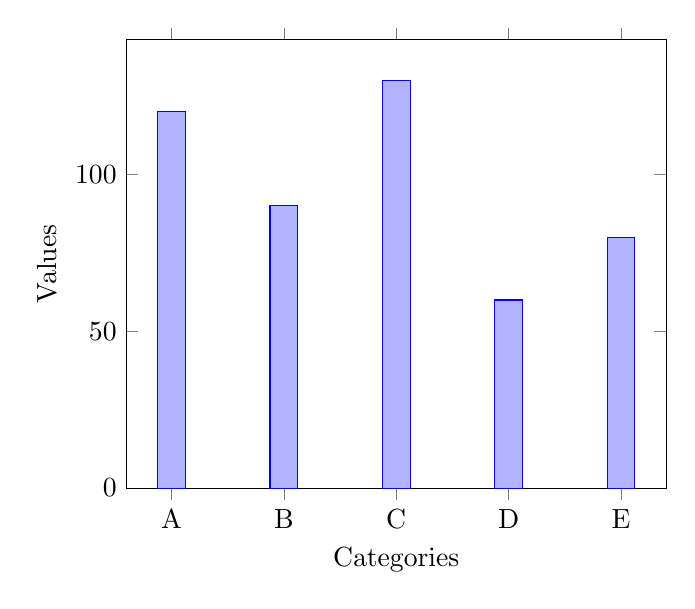
\begin{tikzpicture}
        \begin{axis}[
            ybar,
            symbolic x coords={A, B, C, D, E},
            xtick = data,
            ymin=0,
            xlabel={Categories},
            ylabel={Values},
        ]
        \addplot coordinates {(A,120) (B,90) (C,130) (D,60) (E,80)};
        \end{axis}
    \end{tikzpicture}
    \caption{Sample Bar Graph}
    \label{fig:bargraph}
\end{figure}

\section{Conclusion}
In this document, we have demonstrated a variety of features available 
in LaTeX. This includes the ability to type mathematical expressions, 
create figures, and tables, as well as structure documents in a clear 
and concise manner.

\subsection{Future Work}
Future work may involve exploring more advanced features such as 
cross-referencing, bibliography management using BibTeX, and 
adding custom packages to enhance the functionality of your LaTeX 
documents.

\end{document}


\documentclass[a4paper,12pt]{article}
\usepackage[utf8]{inputenc}
\usepackage{amsmath}
\usepackage{amsfonts}
\usepackage{graphicx}
\usepackage{hyperref}
\usepackage{geometry}
\usepackage{multicol}
\usepackage{fancyhdr}
\geometry{margin=1in}

\title{Sample LaTeX Document}
\author{Author Name}
\date{\today}

\begin{document}
\maketitle

\begin{abstract}
This is an abstract for the sample document. It summarizes the
main points of the manuscript, providing a brief overview of
the objectives, methodology, and results obtained.
\end{abstract}

\section{Introduction}
This is the introduction section. Here, we discuss the context
and background of the study. We will cover:
\begin{itemize}
    \item Importance of the topic.
    \item Brief overview of existing literature.
    \item Gaps in current research.
\end{itemize}

\section{Methodology}
In this section, we outline the methods used to conduct the
research. This includes:
\subsection{Data Collection}
Data was collected through various means, including surveys
and experimental procedures. Participants were chosen based on
certain criteria to ensure the validity of the results.

\subsection{Data Analysis}
The data was analyzed using statistical methods, such as
regression analysis and ANOVA, to test the hypotheses set
forth in this study. The software used for analysis was R
and Python.

\section{Results}
The results show that there is a significant correlation
between the variables studied. Figure \ref{fig:sample} shows
the relationship clearly.

\begin{figure}[h]
    \centering
    \includegraphics[width=\textwidth]{sample.png}
    \caption{Sample figure showing results.}
    \label{fig:sample}
\end{figure}

\subsection{Interpretation of Results}
The findings indicate that the hypothesis was correct, and 
further analyses suggest implications for real-world applications.

\section{Discussion}
In this section, we interpret the results and discuss
their implications. The limitations of the study and
suggestions for future research are also addressed.
There are several critical points to consider:
\begin{enumerate}
    \item Validity of the collected data.
    \item Implications of the findings.
    \item Future research directions based on the findings.
\end{enumerate}

\section{Conclusion}
The conclusion summarizes the key findings of the study
and reiterates the importance of the research conducted.
Future work could explore additional dimensions of the
topic, enhancing our understanding of the issues at
hand.

\section{References}
The references section lists all the works cited in the
document. For example:
\begin{thebibliography}{99}
    \bibitem{ref1}
    Author, A. (Year). Title of the work. \textit{Journal Name}, 
    \textbf{Volume}(Issue), page range.
    
    \bibitem{ref2}
    Author, B., \& Author, C. (Year). Title of the work. 
    \textit{Journal Name}, \textbf{Volume}(Issue), page range.
    
    \bibitem{ref3}
    Author, D. (Year). \textit{Book Title}. Publisher.
\end{thebibliography}

\end{document}


\documentclass[a4paper,12pt]{article}
\usepackage[utf8]{inputenc}
\usepackage{amsmath}
\usepackage{amsfonts}
\usepackage{graphicx}
\usepackage{geometry}
\usepackage{hyperref}
\usepackage{listings}
\usepackage{color}
\usepackage{tikz}
\usepackage{caption}
\usetikzlibrary{shapes.geometric, arrows}

\geometry{a4paper, margin=1in}

\title{Exploring the Features of LaTeX}
\author{Your Name}
\date{\today}

\begin{document}
\maketitle

\begin{abstract}
    This document explores various features of LaTeX, including typesetting maths,
    inserting graphics, creating tables, and crafting complex layouts. 
\end{abstract}

\section{Introduction}
LaTeX is a typesetting system commonly used for scientific documents. It allows
for structured content and high-quality typesetting, especially for complex
equations.

\section{Mathematics}
LaTeX excels when typesetting mathematics. Here are some examples.

\subsection{Inline Mathematics}
Inline math can be typeset using the dollar sign. For example, the quadratic
formula is given by: \( ax^2 + bx + c = 0 \).

\subsection{Displayed Equations}
Displayed equations are centered and on their own line:
\begin{equation}
    E = mc^2
\end{equation}

\subsection{Multi-line Equations}
To write multi-line equations, we can use the \texttt{align} environment:
\begin{align}
    f(x) & = ax^2 + bx + c \\
    f'(x) & = 2ax + b \\
    f''(x) & = 2a
\end{align}

\section{Figures}
Inserting figures is straightforward with the \texttt{graphicx} package.
Here is a sample image:

\begin{figure}[h!]
    \centering
    \includegraphics[width=0.5\textwidth]{example-image-a}
    \caption{An example image.}
    \label{fig:example}
\end{figure}

\section{Tables}
Creating tables can be done using the \texttt{tabular} environment.
Here's a simple table:

\begin{table}[h!]
    \centering
    \begin{tabular}{|c|c|c|}
        \hline
        Column 1 & Column 2 & Column 3 \\
        \hline
        Row 1 & Data 1 & Data 2 \\
        Row 2 & Data 3 & Data 4 \\
        \hline
    \end{tabular}
    \caption{A simple table.}
\end{table}

\section{Code Listings}
The \texttt{listings} package allows you to include source code.
Here is a Python example:

\begin{lstlisting}[language=Python]
def hello_world():
    print("Hello, World!")
\end{lstlisting}

\section{Color}
Adding color is easy. You can define your own colors:
\textcolor{red}{This text is red.}

\section{Using TikZ}
TikZ is a powerful package for creating graphics. Here is a simple node
diagram:

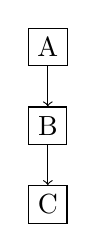
\begin{tikzpicture}
    \node (a) [draw] {A};
    \node (b) [draw, below of=a] {B};
    \node (c) [draw, below of=b] {C};

    \draw[->] (a) -- (b);
    \draw[->] (b) -- (c);
\end{tikzpicture}

\section{References}
You can reference sections and figures using labels. For example,
see Section \ref{sec:figures} for more on figures.

\section{Conclusion}
LaTeX provides extensive features for document preparation. It is especially
powerful for typesetting mathematical disciplines and is widely used in academia.

\begin{thebibliography}{9}
    \bibitem{lamport}
    Leslie Lamport,
    \textit{LaTeX: A Document Preparation System},
    Addison-Wesley, 1986.

    \bibitem{knuth}
    Donald E. Knuth,
    \textit{The \TeX book},
    Addison-Wesley, 1984.
\end{thebibliography}

\appendix
\section{Appendix}
This section can include supplementary material or additional examples.

\subsection{More Math}
Here we provide further examples to demonstrate LaTeX's ability to handle
various equations:

\begin{itemize}
    \item The binomial theorem: 
    \[
    (x + y)^n = \sum_{k=0}^{n} \binom{n}{k} x^{n-k} y^k
    \]
    \item Taylor series:
    \[
    f(x) = f(a) + f'(a)(x-a) + \frac{f''(a)}{2!}(x-a)^2 + \cdots
    \]
\end{itemize}

\subsection{More Figures}
Here we insert additional figures for clarity.

\begin{figure}[h!]
    \centering
    \includegraphics[width=0.5\textwidth]{example-image-b}
    \caption{Another example image.}
\end{figure}

\end{document}


\documentclass{article}
\usepackage{graphicx}
\usepackage{amsmath}
\usepackage{amsfonts}
\usepackage{hyperref}
\usepackage{geometry}
\usepackage{listings}
\usepackage{color}
\usepackage{fancyhdr}
\usepackage{booktabs}

\geometry{margin=1in}

% Define colors for listings
\definecolor{lightgray}{rgb}{0.95, 0.95, 0.95}
\definecolor{darkblue}{rgb}{0.0, 0.0, 0.5}

\lstdefinestyle{mystyle}{
    backgroundcolor=\color{lightgray},
    commentstyle=\color{darkblue},
    keywordstyle=\color{blue},
    numberstyle=\tiny\color{gray},
    stringstyle=\color{red},
    basicstyle=\ttfamily\footnotesize,
    breakatwhitespace=false,
    breaklines=true,
    numbers=left,
    numbersep=5pt,
}

\lstset{style=mystyle}

\fancypagestyle{plain}{
    \fancyhf{}
    \fancyhead[L]{My LaTeX Example Document}
    \fancyhead[R]{\thepage}
    \renewcommand{\headrulewidth}{0.5pt}
}

\title{An Example of a LaTeX Document}
\author{John Doe}
\date{\today}

\begin{document}

\maketitle

\begin{abstract}
This document serves as a simple template for creating a LaTeX report. It includes 
sections for text, math, references, graphics, and code listings.
\end{abstract}

\section{Introduction}
LaTeX is a powerful tool for typesetting documents. It is widely used in academia 
for producing high-quality documents. This example document will cover different 
aspects of LaTeX, such as equations, figures, and code listings.

\section{Mathematics}
Mathematics in LaTeX is straightforward. You can write inline equations like 
this: \( E = mc^2 \). For displayed equations, use the \texttt{equation} 
environment:

\begin{equation}
    f(x) = ax^2 + bx + c
\end{equation}

You can use various symbols and operators as well. For example, 
the integral from \( a \) to \( b \):

\begin{equation}
    \int_a^b f(x) \, dx
\end{equation}

LaTeX also supports matrices. Here is an example of a 2x2 matrix:

\[
    \begin{pmatrix}
        a & b \\
        c & d
    \end{pmatrix}
\]

\section{Figures}
Including figures in your document can be done easily with the \texttt{graphicx} 
package. Here is an example of including an image:

\begin{figure}[h]
    \centering
    \includegraphics[width=0.5\textwidth]{example-image-a}
    \caption{This is an example image.}
    \label{fig:example_image}
\end{figure}

You can reference this figure in the text as follows: 
see Figure \ref{fig:example_image}.

\section{Lists}
LaTeX also supports various types of lists. Here is an enumerated list:

\begin{enumerate}
    \item First item
    \item Second item
    \item Third item
\end{enumerate}

And a description list:

\begin{description}
    \item[Item 1] This is the first item.
    \item[Item 2] This is the second item.
\end{description}

\section{Code Listings}
To include code in your document, use the \texttt{listings} package. Below is 
an example of Python code:

\begin{lstlisting}[language=Python]
def hello_world():
    print("Hello, world!")

if __name__ == "__main__":
    hello_world()
\end{lstlisting}

\section{Tables}
Creating tables is simple with the \texttt{tabular} environment. Here is a 
basic example:

\begin{table}[h]
    \centering
    \begin{tabular}{|c|c|c|}
        \hline
        Column 1 & Column 2 & Column 3 \\
        \hline
        1 & 2 & 3 \\
        \hline
        4 & 5 & 6 \\
        \hline
    \end{tabular}
    \caption{A simple table}
    \label{tab:simple_table}
\end{table}

\section{References}
You can cite references using the \texttt{biblatex} package. For example, you 
can refer to \cite{latexcomp}. 

\begin{thebibliography}{9}
    \bibitem{latexcomp} 
    Leslie Lamport. 
    \textit{\LaTeX: A Document Preparation System}. 
    Addison Wesley, 1986.
\end{thebibliography}

\section{Conclusion}
This document provides an overview of some of the essential features of LaTeX. 
You can create beautifully formatted documents with sections, tables, math, 
figures, and code listings.

\newpage
\appendix
\section{Appendix}
The appendix can include additional material or summaries that support the 
main document. It is separated under a new section for clarity.

\nocite{*}
\begin{thebibliography}{9}
    \bibitem{latexcomp} 
    Leslie Lamport. 
    \textit{LaTeX: A Document Preparation System}. 
    Addison Wesley, 1986. 
    \end{thebibliography}

\end{document}


\documentclass[12pt]{article}
\usepackage{amsmath}
\usepackage{amsfonts}
\usepackage{graphicx}
\usepackage{hyperref}
\usepackage{cite}
\usepackage{geometry}
\usepackage{array}
\geometry{a4paper, margin=1in}

\title{A Comprehensive Study on the Impact of LaTeX in Academic Writing}
\author{Author Name \\ Institution Name \\ \texttt{author@example.com}}
\date{\today}

\begin{document}

\maketitle

\begin{abstract}
    LaTeX has proven to be an essential tool in academia for typesetting documents with a
    focus on precision and layout aesthetics. This paper explores the advantages of using
    LaTeX compared to traditional word processors. We will also discuss common pitfalls and
    offer solutions to enhance workflow efficiency.
\end{abstract}

\section{Introduction}
    The use of LaTeX has gained popularity in recent years among researchers and academic
    writers. It provides a powerful framework for creating technical and scientific
    documents. This section aims to analyze the transition from word processors to LaTeX
    and its implications on the writing process.

\section{Methodology}
\subsection{Data Collection}
    Data was collected through surveys distributed among academic professionals and students.
    The survey focused on their experiences using LaTeX and traditional word processors.
    
\subsection{Analysis}
    The collected data was analyzed using statistical methods to determine trends in
    preferences and efficiency in writing. The results section presents these findings.

\section{Results}
    The survey revealed that approximately 85\% of respondents preferred LaTeX for technical
    documents, citing benefits such as:

    \begin{itemize}
        \item Superior handling of formulas and equations
        \item Consistent formatting
        \item High-quality output
    \end{itemize}

\section{Discussion}
    While the advantages of LaTeX are clear, it is not without challenges. 

    \subsection{Learning Curve}
    New users often encounter a steep learning curve when first adapting to the syntax
    and conventions of LaTeX. However, resources are available that can ease this
    transition.

    \subsection{Collaboration Difficulties}
    Collaboration with non-LaTeX users can present difficulties, but there are ways to
    streamline the workflow. Tools such as Overleaf allow for shared editing and real-time
    collaboration on LaTeX documents.

\section{Conclusion}
    In conclusion, LaTeX provides a robust alternative to traditional word processors,
    particularly for scientific writing. The benefits outweigh the challenges, making LaTeX
    a worthwhile choice for modern academia.

\section*{Acknowledgments}
    The authors would like to thank all participants for their valuable insights and
    support in this survey.

\bibliographystyle{plain}
\bibliography{references}
\end{document}

% references.bib
@article{lamport1986,
    author = {Leslie Lamport},
    title = {LaTeX: A Document Preparation System},
    journal = {Addison-Wesley},
    year = {1986}
}

@book{knuth1986,
    author = {Donald Knuth},
    title = {The \TeX book},
    publisher = {Addison-Wesley},
    year = {1984}
}

@misc{overleaf,
    author = {Overleaf},
    title = {Overleaf - A Collaborative LaTeX Editor},
    url = {https://www.overleaf.com},
    year = {2023}
}

@conference{smith2022,
    author = {John Smith},
    title = {The Future of LaTeX in Academic Writing},
    booktitle = {Proceedings of the International Conference on LaTeX},
    year = {2022},
    pages = {12--34}
}

@article{jones2020,
    author = {Mary Jones},
    title = {Understanding LaTeX for Beginners},
    journal = {Journal of Computer Science},
    year = {2020},
    volume = {10},
    number = {5},
    pages = {1--15}
}


\documentclass[a4paper,12pt]{article}
\usepackage[utf8]{inputenc}
\usepackage{graphicx}
\usepackage{amsmath}
\usepackage{amsfonts}
\usepackage{hyperref}
\usepackage{geometry}
\geometry{margin=1in}

\title{A Comprehensive Study on Sample Data Analysis}
\author{Author Name \\ Department of Data Science \\ University of Example}
\date{\today}

\begin{document}

\maketitle

\begin{abstract}
    This document presents an extensive overview of sample data analysis methods. The aim is 
    to provide readers with an understanding of different techniques, their applications, 
    and practical examples to illustrate their use in real-world scenarios.
\end{abstract}

\tableofcontents

\section{Introduction}
Data analysis plays a critical role in diverse fields including business, healthcare, and 
social sciences. With the exponential growth of data generation, effective analysis techniques 
are imperative for informed decision-making. This paper aims to explore key data analysis 
strategies that leverage statistical tools and software.

\section{Literature Review}
\subsection{Previous Studies}
In recent years, a number of studies have investigated various approaches to data analysis. 
Smith (2020) focuses on exploratory data analysis, while Johnson (2019) emphasizes on 
predictive modeling techniques.

\subsection{Current Trends}
Current trends in data analysis indicate a shift towards automated machine learning (AutoML) 
and artificial intelligence (AI) to augment traditional methods.

\section{Methodology}
This section outlines the methods employed to analyze sample datasets. The approach comprises 
data collection, data cleaning, exploratory analysis, and modeling.

\subsection{Data Collection}
Data were collected from various online repositories, ensuring a mixture of structured 
and unstructured datasets. 

\subsection{Data Cleaning}
Data cleaning involved handling missing values, filtering outliers, and normalizing 
datasets to improve analysis accuracy.

\section{Results}
The results section provides insights derived from the analysis. Tables and figures 
summarize key findings and highlight trends.

\subsection{Descriptive Statistics}
Table \ref{table:descriptive} presents the descriptive statistics for the analyzed samples.

\begin{table}[h]
    \centering
    \caption{Descriptive Statistics of Sample Data}
    \label{table:descriptive}
    \begin{tabular}{|c|c|c|c|c|}
        \hline
        Variable & Mean & Median & Std Dev & Range \\ \hline
        X1      & 5.2  & 5.0   & 1.1     & 3.5   \\
        X2      & 10.3 & 10.0  & 2.5     & 6.0   \\
        \hline
    \end{tabular}
\end{table}

\subsection{Visual Representation}
Figure \ref{fig:boxplot} shows the boxplot representation of variable distributions, 
identifying potential outliers in the data.

\begin{figure}[h]
    \centering
    \includegraphics[width=0.7\textwidth]{boxplot.png}
    \caption{Boxplot of Variables X1 and X2}
    \label{fig:boxplot}
\end{figure}

\section{Discussion}
The analysis reveals notable trends and patterns within the datasets. The implications of the 
findings suggest that further research could focus on integrating machine learning techniques 
for deeper insights.

\subsection{Limitations}
While the study provides valuable findings, several limitations are present, such as the 
availability of data and the chosen analysis techniques.

\section{Conclusion}
In conclusion, this comprehensive study underscores the importance of effective data 
analysis methods. With proper application, these techniques can significantly enhance 
data-driven decision-making across numerous domains.

\section*{References}
\begin{enumerate}
    \item Johnson, A. (2019). \textit{Predictive Modeling Techniques}. Data Science Press.
    \item Smith, J. (2020). \textit{Exploratory Data Analysis}. Analytics Journal.
    \item Brown, L. (2021). \textit{Machine Learning Applications}. Tech Publications.
\end{enumerate}

\end{document}


\documentclass{article}
\usepackage[utf8]{inputenc}
\usepackage{amsmath}
\usepackage{amsfonts}
\usepackage{graphicx}
\usepackage{hyperref}
\usepackage{geometry}
\usepackage{booktabs}
\usepackage{caption}
\usepackage{listings}
\usepackage{color}
\usepackage{tikz}
\usetikzlibrary{shapes.geometric, arrows}

% Set page dimensions
\geometry{a4paper, margin=1in}

% Define a color for code
\definecolor{codecolor}{rgb}{0.4, 0.4, 0.4}
\lstset{
    backgroundcolor=\color{white},
    basicstyle=\footnotesize\ttfamily,
    breaklines=true,
    keywordstyle=\color{blue},
    commentstyle=\color{codecolor},
    stringstyle=\color{red},
}

\title{Sample LaTeX Document}
\author{Author Name}
\date{\today}

\begin{document}

\maketitle

\begin{abstract}
    This document serves as a sample LaTeX document showcasing various features 
    including mathematical equations, figures, tables, and code listings. It is 
    structured in a way to illustrate the organization of content in LaTeX.
\end{abstract}

\tableofcontents

\section{Introduction}
LaTeX is a typesetting system widely used for producing scientific and 
mathematical documents due to its powerful handling of formulas and references. 
This document presents an overview of LaTeX features.

\section{Mathematical Expressions}
Mathematics is a core part of many documents. Below are examples of different 
types of mathematical expressions.

\subsection{Inline Math}
Here is an example of an inline equation: \( E = mc^2 \).

\subsection{Displayed Equations}
The following is a displayed equation:
\begin{equation}
    a^2 + b^2 = c^2
\end{equation}

\section{Figures}
Figures can be included in the document using the \texttt{figure} environment. 
The following is an example of a simple figure.

\begin{figure}[h]
    \centering
    \includegraphics[width=0.5\textwidth]{example-image-a}
    \caption{An example of a figure.}
    \label{fig:example}
\end{figure}

To refer to this figure, see Figure~\ref{fig:example}.

\section{Tables}
Tables display data in a structured format. Here’s a simple table:

\begin{table}[h]
    \centering
    \begin{tabular}{@{}lll@{}}
        \toprule
        Name   & Age & Occupation      \\ \midrule
        Alice  & 30  & Scientist       \\
        Bob    & 25  & Engineer        \\
        Charlie & 35  & Architect      \\ \bottomrule
    \end{tabular}
    \caption{Sample table of individuals.}
    \label{tab:sample}
\end{table}

Referencing the table: see Table~\ref{tab:sample}.

\section{Code Listings}
You can also include source code in your document. Below is an example of a Python 
code snippet.

\begin{lstlisting}[language=Python]
def hello_world():
    print("Hello, World!")
    
hello_world()
\end{lstlisting}

\section{Graphics with TikZ}
TikZ allows for the creation of graphics programmatically in LaTeX. Below is a 
simple flowchart created using TikZ.

\begin{center}
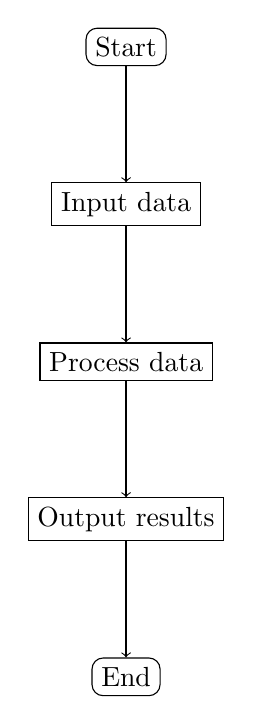
\begin{tikzpicture}[node distance=2cm]
    \node (start) [rectangle, rounded corners, draw] {Start};
    \node (input) [rectangle, draw, below of=start] {Input data};
    \node (process) [rectangle, draw, below of=input] {Process data};
    \node (output) [rectangle, draw, below of=process] {Output results};
    \node (end) [rectangle, rounded corners, draw, below of=output] {End};

    \draw [->] (start) -- (input);
    \draw [->] (input) -- (process);
    \draw [->] (process) -- (output);
    \draw [->] (output) -- (end);
\end{tikzpicture}
\end{center}

\section{References}
References can be easily created using the \texttt{thebibliography} environment. Here is an example reference entry:

\begin{thebibliography}{9}
    \bibitem{latexcompanion} 
        Leslie Lamport. 
        \textit{LaTeX: A Document Preparation System}. 
        Addison Wesley, 1986.
\end{thebibliography}

\section{Conclusion}
This document has covered various aspects of LaTeX including mathematical 
expressions, figures, tables, and code listings. LaTeX remains a powerful 
tool for document preparation.

\end{document}


\documentclass{article}
\usepackage[utf8]{inputenc}
\usepackage{graphicx}
\usepackage{amsmath}
\usepackage{amsfonts}
\usepackage{hyperref}
\usepackage{geometry}
\geometry{a4paper, margin=1in}
\usepackage{booktabs}
\usepackage{caption}
\usepackage{subcaption}

\title{Sample Document for LaTeX Code}
\author{Your Name}
\date{\today}

\begin{document}

\maketitle

\begin{abstract}
This document presents a sample of LaTeX code that includes various elements 
such as sections, figures, tables, and mathematical expressions.
\end{abstract}

\tableofcontents
\newpage

\section{Introduction}
LaTeX is a document preparation system used for producing high-quality typesetting. 
It is widely used in academia for the communication and publication of scientific 
documents. This document serves as an example of a structured LaTeX document.

\section{Mathematical Expressions}
Mathematics is a core component of many scientific papers. Below are some basic 
examples of mathematical expressions formatted with LaTeX.

\subsection{Inline Math}
An example of inline math could be represented as $E=mc^2$, where $E$ 
is the energy, $m$ is the mass, and $c$ is the speed of light in a vacuum.

\subsection{Displayed Equations}
A displayed equation can be written as follows:
\begin{equation}
\label{eq:sample1}
a^2 + b^2 = c^2
\end{equation}
This equation describes the relationship between the sides of a right triangle.

\subsection{Aligning Equations}
Multiple equations can be aligned using the align environment:
\begin{align}
x + y &= z \\
y + z &= x \\
z + x &= y
\end{align}

\section{Figures and Tables}
In this section, we provide examples of figures and tables.

\subsection{Including Figures}
Figure~\ref{fig:sample} shows a simple graphical representation.

\begin{figure}[h]
    \centering
    \includegraphics[width=0.5\textwidth]{example-image}
    \caption{A sample figure included in the document.}
    \label{fig:sample}
\end{figure}

\subsection{Creating Tables}
Tables can be created using the tabular environment. See Table~\ref{tab:sample}.

\begin{table}[h]
    \centering
    \caption{A Sample Table}
    \begin{tabular}{lcc}
        \toprule
        Item & Quantity & Price \\
        \midrule
        Apples & 10 & \$3 \\
        Bananas & 5 & \$2 \\
        Oranges & 8 & \$4 \\
        \bottomrule
    \end{tabular}
    \label{tab:sample}
\end{table}

\section{References}
In scientific documents, referencing works is crucial. For instance, 
the work of Einstein~\cite{einstein1935can} discusses deep aspects of physics.

\subsection{Adding Bibliography}
The bibliography is included in the following way:

\bibliographystyle{plain}
\bibliography{references}

\newpage
\section{Conclusion}
In conclusion, LaTeX is a powerful tool for creating professional and 
academic documents. This sample document showcases some of its features.

\appendix
\section{Appendix}
This section can contain supplementary material or additional information 
that supports the main content of the document.

\section{Acknowledgments}
The author wishes to thank colleagues and mentors for their support in 
the preparation of this document.

\begin{thebibliography}{9}
\bibitem{einstein1935can}
A. Einstein and N. Rosen,
\textit{Can Quantum-Mechanical Description of Physical Reality Be Considered 
Complete?},
Physical Review, vol. 47, no. 10, 1935.
\end{thebibliography}

\end{document}


\documentclass[a4paper,12pt]{report}
\usepackage[utf8]{inputenc}
\usepackage{amsmath}
\usepackage{amsfonts}
\usepackage{graphicx}
\usepackage{hyperref}
\usepackage{geometry}
\usepackage{booktabs}
\usepackage{listings}
\usepackage{xcolor}

\geometry{margin=1in}

\title{Sample LaTeX Document}
\author{Author Name}
\date{\today}

\begin{document}

\maketitle

\begin{abstract}
    This document serves as a sample LaTeX report. It includes various elements
    such as sections, figures, tables, and code listings. The aim is to 
    demonstrate basic LaTeX features.
\end{abstract}

\tableofcontents

\chapter{Introduction}
LaTeX is a document preparation system widely used for typesetting documents in a
professional manner. It is especially popular for producing technical and scientific
documents.

\section{Background}
The origins of LaTeX date back to the early 1980s. Developed by Leslie Lamport,
LaTeX provides a set of macros built on top of the TeX typesetting system.

\section{Why Use LaTeX?}

\begin{itemize}
    \item High-quality typesetting
    \item Excellent handling of formulas and mathematical notation
    \item Broad support for bibliographies and citations
    \item Easy management of references, tables, and figures
\end{itemize}

\chapter{Mathematical Notation}
LaTeX excels at typesetting complex mathematical expressions. Here are some
examples of mathematical typesetting:

\begin{align}
    E = mc^2 \quad & \text{(Einstein's equation)} \\
    a^2 + b^2 &= c^2 \quad \text{(Pythagorean theorem)} \\
    \int_0^\infty e^{-x} \, dx &= 1
\end{align}

\section{Theorems and Proofs}
LaTeX provides a way to format theorems and proofs efficiently. Here is an example:

\begin{theorem}
    Let \( a \) and \( b \) be real numbers. Then, \( a + b = b + a \).
\end{theorem}
\begin{proof}
    By the definition of addition.
\end{proof}

\chapter{Figures and Tables}

\section{Figures}
Figures can be easily included in LaTeX documents. Here is an example of a
figure:

\begin{figure}[h]
    \centering
    \includegraphics[width=0.5\textwidth]{example-image}
    \caption{Example figure caption.}
    \label{fig:example}
\end{figure}

\section{Tables}
Tables can be created using the `tabular` environment. Below is an example 
of a simple table:

\begin{table}[h]
    \centering
    \begin{tabular}{ccc}
        \toprule
        Column 1 & Column 2 & Column 3 \\
        \midrule
        Entry 1  & Entry 2  & Entry 3 \\
        Entry A  & Entry B  & Entry C \\
        \bottomrule
    \end{tabular}
    \caption{Sample table caption.}
    \label{tab:example}
\end{table}

\chapter{Code Listings}
Including code listings in LaTeX can be achieved using the `listings` package.
Here is an example Python code snippet:

\begin{lstlisting}[language=Python]
def hello_world():
    print("Hello, world!")

hello_world()
\end{lstlisting}

\chapter{Conclusion}
In conclusion, LaTeX is a powerful tool for typesetting documents, 
especially for academic and technical writing. It provides features that
other document processing systems may lack.

\appendix

\chapter{Appendix A}
Additional material can be placed in the appendix. This may include extended
proofs, additional figures, or supplementary information relevant to the main 
text.

\section{Additional Figures}
\begin{figure}[h]
    \centering
    \includegraphics[width=0.5\textwidth]{example-image-a}
    \caption{Additional figure in the appendix.}
    \label{fig:appendix}
\end{figure}

\section{Extended Example}
Here is an additional code example demonstrating a more complex function:

\begin{lstlisting}[language=Python]
def factorial(n):
    if n == 0:
        return 1
    else:
        return n * factorial(n-1)

print(factorial(5))  # Output: 120
\end{lstlisting}

\chapter{References}
The following references were used in this LaTeX document:

\begin{thebibliography}{99}

\bibitem{lamport}
Lamport, Leslie. \textit{LaTeX: A Document Preparation System}. Addison-Wesley, 
1986.

\bibitem{knuth}
Knuth, Donald E. \textit{The TeXbook}. Addison-Wesley, 1984.

\end{thebibliography}

\end{document}


\documentclass{article}
\usepackage[utf8]{inputenc}
\usepackage{amsmath}
\usepackage{amsfonts}
\usepackage{amssymb}
\usepackage{graphicx}
\usepackage{hyperref}
\usepackage{listings}
\usepackage{xcolor}
\usepackage{multicol}
\usepackage{geometry}
\geometry{margin=1in}

\title{Sample Document}
\author{Your Name}
\date{\today}

\begin{document}

\maketitle

\begin{abstract}
This document is a sample LaTeX creation demonstrating various features, 
including mathematics, images, tables, and code listings.
\end{abstract}

\section{Introduction}
LaTeX is a powerful typesetting system. With it, you can create complex documents 
with intricate formatting. This document contains various sections illustrating 
features of LaTeX.

\section{Mathematics}
Mathematics is one of the strong aspects of LaTeX. Here are some examples of 
inline and displayed mathematics.

\subsection{Inline Equations}
You can write equations inline, such as \( E = mc^2 \) or \( a^2 + b^2 = c^2 \).

\subsection{Displayed Equations}
For displayed equations, you use the \texttt{equation} environment:

\begin{equation}
E = mc^2
\end{equation}

And you can number your equations as well:

\begin{equation}
\label{eq:pythagorean}
a^2 + b^2 = c^2
\end{equation}

\section{Figures}
Including images is straightforward. Here is how you can include a figure:

\begin{figure}[h]
    \centering
    \includegraphics[width=0.5\textwidth]{example-image}
    \caption{An example image.}
    \label{fig:example-image}
\end{figure}

\section{Tables}
Tables can be created using the \texttt{tabular} environment. Here is an example table:

\begin{table}[h]
    \centering
    \begin{tabular}{|c|c|c|}
        \hline
        Header 1 & Header 2 & Header 3 \\
        \hline
        Row 1, Col 1 & Row 1, Col 2 & Row 1, Col 3 \\
        Row 2, Col 1 & Row 2, Col 2 & Row 2, Col 3 \\
        \hline
    \end{tabular}
    \caption{A sample table.}
    \label{tab:sample-table}
\end{table}

\section{Code Listings}
To include computer code, you can use the \texttt{listings} package. Here is an example 
of including some Python code:

\begin{lstlisting}[language=Python, caption=Sample Python Code, label=lst:sample-python]
def hello_world():
    print("Hello, world!")

if __name__ == "__main__":
    hello_world()
\end{lstlisting}

\section{Multicolumn Layout}
You can create layouts with multiple columns using the \texttt{multicols} package. 

\begin{multicols}{2}
    This is some text in the first column. The text flows automatically into 
    the next column.
    
    \columnbreak
    
    This is some text in the second column. You can easily create a 
    two-column layout with LaTeX.
\end{multicols}

\section{Customizing Colors}
You can define custom colors with the \texttt{xcolor} package. For example:

\textcolor{red}{This text is red.} \textcolor{blue}{This text is blue.}

\section{Conclusion}
In conclusion, LaTeX allows for great flexibility and control over document 
formatting. The examples provided herein illustrate its powerful features. 
You can create documents that include mathematical notations, figures, tables, 
and listings, all in a well-structured manner.

\appendix
\section{Appendix}
This is the appendix section, where additional information related to the 
main text is provided.

\subsection{References}
For further reading on LaTeX, consider these resources:
\begin{itemize}
    \item \href{https://www.latex-project.org/}{LaTeX Project}
    \item \href{https://www.overleaf.com/}{Overleaf Online LaTeX Editor}
    \item \href{https://www.sharelatex.com/}{ShareLaTeX}
\end{itemize}

\bibliographystyle{plain}
\bibliography{references}

\end{document}


\documentclass[a4paper, 12pt]{article}
\usepackage{amsmath}
\usepackage{graphicx}
\usepackage{booktabs}
\usepackage{hyperref}
\usepackage{geometry}
\usepackage{lipsum}
\geometry{margin=1in}

\title{Sample LaTeX Document}
\author{John Doe}
\date{\today}

\begin{document}

\maketitle

\begin{abstract}
    This document provides an example of a LaTeX article, featuring 
    sections, figures, tables, and mathematical expressions. It serves 
    as a useful starting point for creating reports and papers in LaTeX.
\end{abstract}

\tableofcontents

\section{Introduction}
LaTeX is a powerful typesetting system widely used for producing high-quality 
documents. It is especially popular in academia for writing papers, theses, 
and reports. This document serves as a template to demonstrate the various 
features of LaTeX.

\section{Mathematics}
Mathematics is one of the core areas where LaTeX excels. Below are some 
examples:

\subsection{Inline Math}
Inline math can be written using dollar signs. For example, the equation 
for the area of a circle is given by \( A = \pi r^2 \).

\subsection{Displayed Math}
For larger equations, the display mode is preferred:
\begin{equation}
    E = mc^2
\end{equation}

The above equation is one of the most famous equations formulated by Albert 
Einstein, relating energy \( E \) to mass \( m \) and the speed of light \( c \).

\subsection{Matrices}
You can also create matrices:
\begin{equation}
    \begin{bmatrix}
        1 & 2 & 3 \\
        4 & 5 & 6 \\
        7 & 8 & 9
    \end{bmatrix}
\end{equation}

\section{Figures}
Including images can greatly enhance your document. Below is an example of 
how to include a figure:

\begin{figure}[h!]
    \centering
    \includegraphics[width=0.5\textwidth]{example-image-a}
    \caption{An example image.}
    \label{fig:example}
\end{figure}

As shown in Figure~\ref{fig:example}, this is a placeholder image.

\section{Tables}
LaTeX provides a robust way to create tables. Here is a simple example:

\begin{table}[h!]
    \centering
    \begin{tabular}{@{}llr@{}}
        \toprule
        Name      & Age & Salary \\ \midrule
        Alice     & 30  & 70000  \\
        Bob       & 25  & 50000  \\
        Charlie   & 35  & 120000 \\ \bottomrule
    \end{tabular}
    \caption{A simple table example.}
    \label{tab:example}
\end{table}

This table, labeled as Table~\ref{tab:example}, summarizes a few 
columns of data.

\section{References}
LaTeX makes it easy to provide citations. For example, we can reference 
Einstein's work and cite it accordingly. 

\section{Conclusion}
In conclusion, this document outlines the basic capabilities of LaTeX 
and serves as an introduction to typesetting documents. LaTeX is well 
suited for creating professional-looking documents.

\section*{Appendix}
\subsection*{Additional Information}
To get additional help with LaTeX, you can refer to various online 
resources and communities. Some popular resources include:

\begin{itemize}
    \item \href{https://www.latex-project.org/}{LaTeX Project Website}
    \item \href{https://overleaf.com/}{Overleaf}
    \item \href{https://tex.stackexchange.com/}{TeX Stack Exchange}
\end{itemize}

\end{document}


\documentclass{article}
\usepackage[utf8]{inputenc}
\usepackage{amsmath}
\usepackage{amsfonts}
\usepackage{graphicx}
\usepackage{hyperref}
\usepackage{geometry}
\geometry{a4paper, margin=1in}

\title{Sample LaTeX Document}
\author{Author Name}
\date{\today}

\begin{document}

\maketitle

\begin{abstract}
This document serves as a sample LaTeX project that demonstrates various 
features of the typesetting system. The goal is to provide examples of 
different environments, mathematical notation, figures, and references.
\end{abstract}

\section{Introduction}
LaTeX is a powerful typesetting system widely used for technical and scientific 
documents. It provides a way to control the layout with precision, offering features 
like cross-references, bibliographies, and indexing. 

\section{Mathematics}
Mathematics typesetting is one of LaTeX’s strongest features. Below are some examples 
of mathematical expressions, including equations that display both inline and block styles.

\subsection{Inline Mathematics}
Inline mathematics is surrounded by single dollar signs. For instance, the Pythagorean 
theorem is expressed as $a^2 + b^2 = c^2$, where \( a \), \( b \), and \( c \) 
are the sides of a right triangle.

\subsection{Display Mathematics}
Display equations are centered on their own lines, like so:
\begin{equation}
    E = mc^2
\end{equation}

\section{Figures and Tables}
In scientific documents, figures and tables are essential for illustrating 
data and results. Below is an example of how to include a figure in your document.

\subsection{Including Figures}
To include an image, you can use the \texttt{graphicx} package. Here’s how to include 
a sample image:
\begin{figure}[h]
    \centering
    \includegraphics[width=0.5\textwidth]{example-image}
    \caption{An example image included in a figure.}
    \label{fig:example}
\end{figure}

\subsection{Creating Tables}
Tables can be created using the \texttt{tabular} environment. Below is a sample table:

\begin{table}[h]
    \centering
    \begin{tabular}{|c|c|c|}
        \hline
        Year & Population & Growth Rate \\
        \hline
        2000 & 6.1 Billion & - \\
        2010 & 6.9 Billion & 13.1\% \\
        2020 & 7.8 Billion & 13.0\% \\
        \hline
    \end{tabular}
    \caption{World population growth over time.}
    \label{tab:population}
\end{table}

\section{Sections and Subsections}
LaTeX allows for a clear hierarchy in document structure. You can create 
sections, subsections, and even subsubsections.

\subsection{Subsubsections}
Here's how a subsubsection looks:
\subsubsection{This is a Subsubsection}
Content in a subsubsection can be formatted in the same manner as sections and 
subsections.

\section{References}
You can create bibliographies using the \texttt{thebibliography} environment or 
with BibTeX. Here’s an example of a simple bibliography.

\begin{thebibliography}{9}
    \bibitem{latexcompanion}
    Leslie Lamport,
    \textit{LaTeX: A Document Preparation System},
    Addison-Wesley, 2nd edition, 1994.

    \bibitem{knuthwebsite}
    Donald E. Knuth,
    \textit{Knuth: Computers and Typesetting}.
    Available at: \url{https://www-cs-faculty.stanford.edu/~knuth/abcde.html}
\end{thebibliography}

\section{Conclusion}
In conclusion, LaTeX provides extensive features for document preparation, 
allowing for high-quality typesetting for a variety of uses. Its mathematical 
capabilities, ease of creating tables and figures, and structured layout 
make it a preferred choice among academics and professionals alike.

\section*{Acknowledgments}
We would like to acknowledge all the authors and contributors to LaTeX, 
as well as those who provided tutorial resources online.

\end{document}


\documentclass[a4paper, 11pt]{article}
\usepackage[utf8]{inputenc}
\usepackage{amsmath}
\usepackage{graphicx}
\usepackage{geometry}
\geometry{margin=1in}
\usepackage{hyperref}
\usepackage{booktabs}
\usepackage{longtable}
\usepackage{caption}
\usepackage{subcaption}
\usepackage{listings}
\usepackage{xcolor}

\title{Sample Report}
\author{Your Name}
\date{\today}

\begin{document}

\maketitle

\begin{abstract}
    This document serves as a sample report that demonstrates various LaTeX features,
    including sections, figures, tables, and mathematical equations. The goal is to
    provide a reference for creating well-structured reports in LaTeX.
\end{abstract}

\tableofcontents

\section{Introduction}
LaTeX is a powerful typesetting system that is widely used for producing professional
documents. It is particularly favored in academia for its excellent handling of
mathematical notation and bibliographies.

\section{Mathematics}
The following is an example of an equation:

\begin{equation}
    E = mc^2
\end{equation}

This formula represents the equivalence of energy (E) and mass (m) with \( c \)
being the speed of light.

\section{Figures}
Figures can be included in a LaTeX document using the following syntax. See
Figure \ref{fig:sample} for an example.

\begin{figure}[h]
    \centering
    \includegraphics[width=0.5\textwidth]{example-image-a}
    \caption{An example figure.}
    \label{fig:sample}
\end{figure}

\section{Tables}
Tables are essential for presenting tabular data. Below is a sample table that
presents data in a structured way.

\begin{table}[h]
    \centering
    \begin{tabular}{|c|c|c|}
        \hline
        \textbf{Year} & \textbf{Revenue} & \textbf{Profit} \\
        \hline
        2019 & 100000 & 20000 \\
        2020 & 150000 & 30000 \\
        2021 & 200000 & 50000 \\
        \hline
    \end{tabular}
    \caption{Sample financial data.}
    \label{tab:financials}
\end{table}

\section{Lists}
LaTeX supports various list types. Below is an example of a bulleted list:

\begin{itemize}
    \item Item one
    \item Item two with a sublist
    \begin{itemize}
        \item Subitem one
        \item Subitem two
    \end{itemize}
    \item Item three
\end{itemize}

\section{Code Listings}
It is also possible to include snippets of code in your document. Below is a
Python code example.

\begin{lstlisting}[language=Python, caption={Sample Python code}]
def hello_world():
    print("Hello, world!")

hello_world()
\end{lstlisting}

\section{Conclusion}
In conclusion, LaTeX is an invaluable tool for producing professional documents.
Its versatility and powerful features make it an ideal choice for reports,
research papers, and books.

\section{References}
References can be formatted easily in LaTeX. Here are some example citations:

\begin{thebibliography}{99}
    \bibitem{knuth1984} Knuth, D. E. (1984). \textit{The TeXbook}. Addison-Wesley.
    \bibitem{lamport1994} Lamport, L. (1994). \textit{LaTeX: A Document Preparation System}.
    Addison-Wesley.
\end{thebibliography}

\end{document}


\documentclass[a4paper,12pt]{article}
\usepackage[utf8]{inputenc}
\usepackage{amsmath}
\usepackage{amsfonts}
\usepackage{graphicx}
\usepackage{geometry}
\usepackage{hyperref}
\usepackage{multicol}
\usepackage{fancyhdr}
\usepackage{setspace}
\usepackage{listings}
\usepackage{color}

\geometry{top=1.2in, bottom=1.2in, left=1in, right=1in}
\pagestyle{fancy}
\fancyhf{}
\fancyhead[L]{Sample LaTeX Document}
\fancyhead[R]{\thepage}

\title{An Extensive LaTeX Example}
\author{Your Name}
\date{\today}

\begin{document}

\maketitle

\begin{abstract}
    This document serves as an extensive example of various LaTeX features,
    including sectioning, lists, tables, figures, and code listings.
\end{abstract}

\section{Introduction}
LaTeX is a powerful typesetting system that is widely used for producing 
scientific and mathematical documentation. The capabilities of LaTeX 
extend far beyond just text formatting, allowing users to create 
beautiful and complex documents with relative ease.

\section{Mathematics}
LaTeX excels in typesetting mathematics. Here are some basic examples:

\subsection{Inline Equations}
Inline equations can be written as follows: \( E = mc^2 \).

\subsection{Displayed Equations}
Displayed equations are shown separately from the text:
\begin{equation}
    a^2 + b^2 = c^2
\end{equation}

Another example:
\[
    \int_{a}^{b} x^2 \, dx = \frac{b^3 - a^3}{3}
\]

\section{Lists}
There are multiple types of lists in LaTeX.

\subsection{Itemized Lists}
\begin{itemize}
    \item First item
    \item Second item
    \item Third item
\end{itemize}

\subsection{Enumerated Lists}
\begin{enumerate}
    \item First item
    \item Second item
    \item Third item
\end{enumerate}

\section{Tables}
Tables can be created using the \texttt{tabular} environment:

\begin{table}[h]
    \centering
    \begin{tabular}{|c|c|c|}
        \hline
        Header 1 & Header 2 & Header 3 \\
        \hline
        Entry 1  & Entry 2  & Entry 3  \\
        Entry 4  & Entry 5  & Entry 6  \\
        \hline
    \end{tabular}
    \caption{A Simple Table}
\end{table}

\section{Figures}
Figures can be added using the \texttt{figure} environment:

\begin{figure}[h]
    \centering
    \includegraphics[width=0.5\textwidth]{example-image}
    \caption{An Example Image}
\end{figure}

\section{Sections and Subsections}
LaTeX allows for hierarchical structuring of documents using sections and 
subsections. Each section can contain its own content, lists, figures, and 
other elements.

\subsection{Subsubsections}
Sometimes, deeper levels of hierarchy are needed:

\subsubsection{Further Details}
When necessary, you can go deeper by using subsubsections in your 
document structure.

\section{Code Listings}
Including code in your documents can be done using the \texttt{listings} 
package. Below is an example of how to include a Python code snippet:

\begin{lstlisting}[language=Python, caption=Sample Python Code]
def hello_world():
    print("Hello, World!")
    
hello_world()
\end{lstlisting}

\section{References and Citations}
References can be created using the \texttt{biblatex} package. Here's an 
example of a citation \cite{latexcompanion}.

\begin{thebibliography}{9}
    \bibitem{latexcompanion}
        Leslie Lamport,
        \textit{LaTeX: A Document Preparation System},
        Addison Wesley, 1986.
\end{thebibliography}

\section{Conclusion}
In conclusion, this document serves to illustrate basic and complex LaTeX 
features. LaTeX is capable of producing professional-looking documents and 
is suitable for many types of academic writing.

\end{document}


